\section{Procedures for Selecting Background Variables, Estimated Treatment Effects, and Estimated Combining Functions} \label{appendix:results}

\noindent In this appendix we first explain our method for selecting the background variables that we control for when estimating treatment effects.\footnote{This is a separate discussion from the election of variables to forecast life-cycle profiles of labor income and other outcomes. For that discussion see Appendix~\ref{appendix:methodology}.} Then, we present the treatment effects of the center-based treatment in ABC/CARE estimates for the 95 main outcomes we consider. For each set of estimates, we first present a summary of the effect of the program using a combining function counting the number of socially positive treatment effects. We then present tables of treatment effect estimates for each outcome. Finally, we test for statistically significant treatment effects using the step-down procedure to test multiple hypotheses.\\

\subsection{Background Variables} \label{appendix:bvariables}

\noindent We select three out of fourteen potential variables that best predict the relevant outcomes of interest, i.e. the outcomes we test treatment effects for. We list the fourteen variables in Table~\ref{tab:pselectvars} and bold the three we choose. In addition to these three variables, we account for a male indicator when computing estimates pooling males and females and a ABC/CARE indicator, to account for any difference in the programs---although we extensively document throughout the paper the similarities between them. 

\singlespacing
\begin{table}[H]
\centering
\begin{threeparttable}
\caption{Background Variables}
\label{tab:pselectvars}
\begin{tabular}{C{5cm} C{5cm} C{5cm}}
\toprule
\textbf{Maternal IQ}			& \textbf{Maternal education}		& Mother's age at birth \\
High Risk Index		& Parent income			& Premature birth \\
1 minute Apgar score	& 5 minute Apgar score	& Mother married \\
Teen pregnancy		& \textbf{Father at home}			& Number of siblings \\
Cohort 				& Mother is employed		& \\
\bottomrule
\end{tabular}
\begin{tablenotes}
\footnotesize
\item Note: This table lists the variables we permute over when selecting the background variables we control for in our estimations. We bold the variables we choose based on the procedure explained in this section.
\end{tablenotes}
\end{threeparttable}
\end{table}
\doublespacing

\noindent We briefly formalize the choice of the control sets based on most predictive models in the next lines.\\

\noindent Let $\mathcal{M}$ be the set of all the models we consider. In our application, $\mathcal{M}$ consists of all linear regressions of an outcome of interest on the different combinations of background variables. $m \in \mathcal{M}$ is one of such models. We choose the model minimizing the Bayesian Information Criterion (BIC) by ranking them according to their likelihood. That is, according to their posterior probability given the data. The data, in this case, are the dependent variable being predicted together with the background variables in each combination. We denote this by $\Pr( m | \text{Data} )$.\\

\pagebreak
\noindent Using Bayes Rule and the law of total probability,

\begin{eqnarray}
\Pr( m | \text{Data} ) &=& \frac{\Pr(\text{Data} | m)\times \Pr(m)}{ \Pr(\text{Data})}\\ \nonumber
&=& \frac{\Pr(\text{Data} | m)\times \Pr(m)}{\sum \limits _{m' \in M} \Pr (\text{Data} | m') \Pr(m')} \\ \nonumber
&\propto& \Pr (\text{Data} | m) \times \Pr(m),
\end{eqnarray}

\noindent where $\Pr(m)$ is the prior probability of model $m$ and $\Pr(\text{Data} | m)$ is the probability of observing $\text{Data}$ under model $m$.\\

\noindent There are various approaches to rank the the likelihood of each model. Examples include rankings based on Bayesian Information Criterion (Schwarz), the Hannan-Quinn Information Criterion (HWIC), and the Akaike Information Criterion (AIC). We use the first approach because it has appealing consistency properties \citep{Diebold_2007_Forecasting}. This criterion minimizes the following loss function: $2 \log [\Pr( \text{Data} | m)]$. We follow an specific approximation developed by \citet{Claeskens-Hjort_2008_Model-Selection}, which assumes uniform priors and simplifies the computation of the loss function.\\

\noindent This procedure allows us to choose one control set per outcomes of interest. To gain consistency across all specifications, we sum the BIC across all outcomes and choose the background variables with lower average across models. These background variables form our control set across all estimations and appear bold in Table~\ref{tab:pselectvars}.\\

\subsubsection{Matching Variables}\label{app:matching-is-fun}

\noindent We use matching estimators for different versions of the ``treatment vs. stay at home'' and ``treatment vs. alternative preschools'' parameters. For treatment vs. stay at home, we construct the Mahalanobis distance between the individuals in the treatment group and the control group who stay at home and use an Epanechnikov metric to construct an individual-level weight---giving a relatively high weight to individuals in the treatment group who would have been likely to stay at home if randomized to the control group. We proceed analogously when estimating the treatment vs. alternative preschool parameters. We use the same variables to ``match'' and to ``control''.\\

\noindent Other forms of matching estimates such as propensity score matching and nearest neighbor(s) give very similar results and are available upon request. We analyze sensitivity to the choice of controls and matching variables next.\\

\subsubsection{Sensitivity Analysis} \label{app:senscontrols}

\noindent An immediate route of inquiry has to do with the sensitivity of our estimates to the choice of background variables. Especially in the context of our small sample, in which estimates can vary to different model specifications. To investigate this, we estimate treatment effects for the three counterfactuals we consider using all possible control sets for the three variables we can form with the background variables in Table~\ref{tab:pselectvars}. We also consider all possible control sets of one and two variables in Table~\ref{tab:pselectvars}. For brevity, we present this exercise for two outcomes, employment and education. Similar exercises for the 95 main outcomes we consider are available upon request.\\

\noindent Figure~\ref{fig:senstnb} to Figure~\ref{fig:senstap} display the results from this exercise. In any case, the support of the distributions are very compressed leading us to conclude that there is little sensitivity to the choice of controls sets. This is especially true for the comparisons of treatment vs. staying at home and vs. alternative preschool.

\begin{sidewaysfigure}[!htbp]
\centering
\caption{Sensitiviy to Choice of Control Set, Treatment vs. Next Best}\label{fig:senstnb}
\begin{subfigure}[h]{0.4\textwidth}
		\centering
		\caption{Years of Education, Males}
		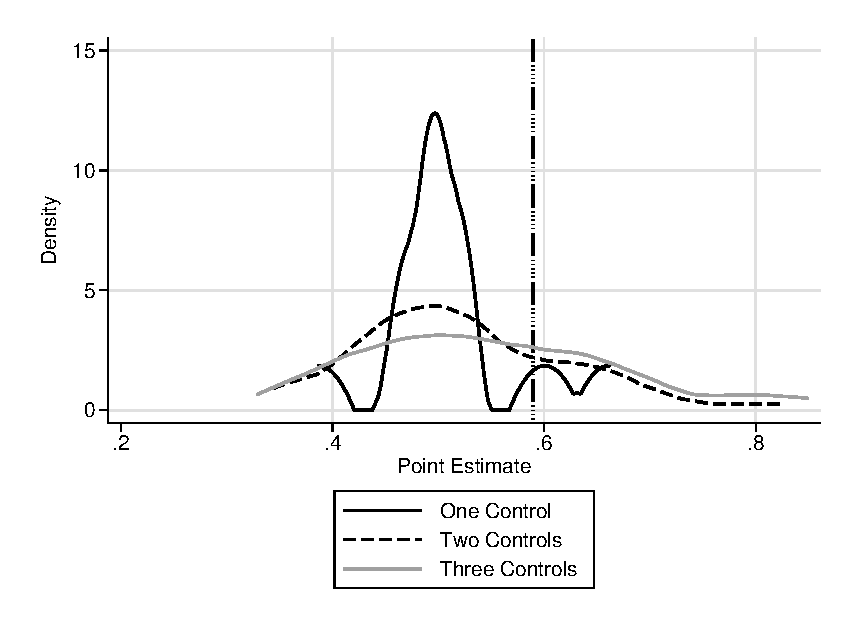
\includegraphics[width=\textwidth]{output/sencontrols_male_years_30y_itt_wctrl.eps}
\end{subfigure}%
\begin{subfigure}[h]{0.4\textwidth}
	\centering
	\caption{Employment, Males}
		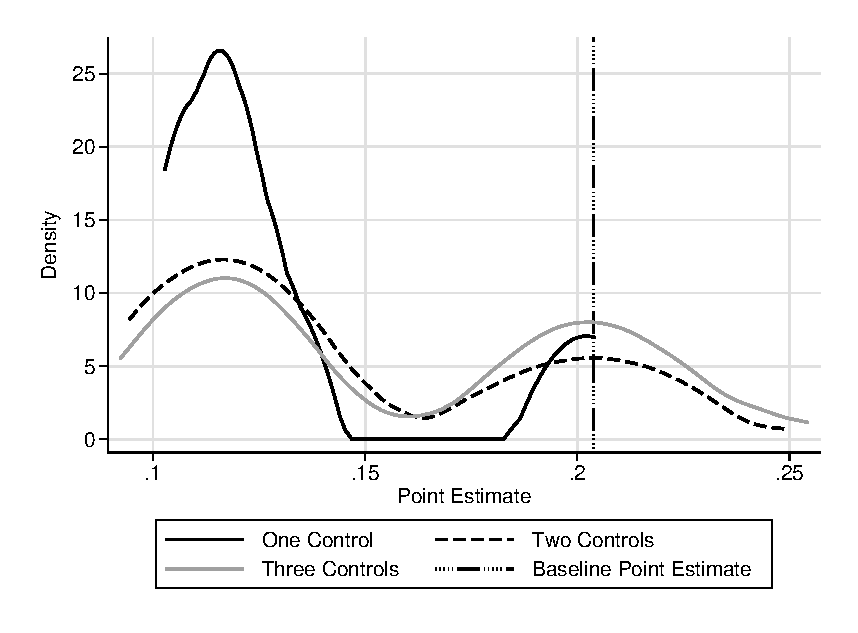
\includegraphics[width=\textwidth]{output/sencontrols_male_si30y_works_itt_wctrl.eps}
\end{subfigure}
\begin{subfigure}[h]{0.4\textwidth}
		\centering
		\caption{Years of Education, Females}
		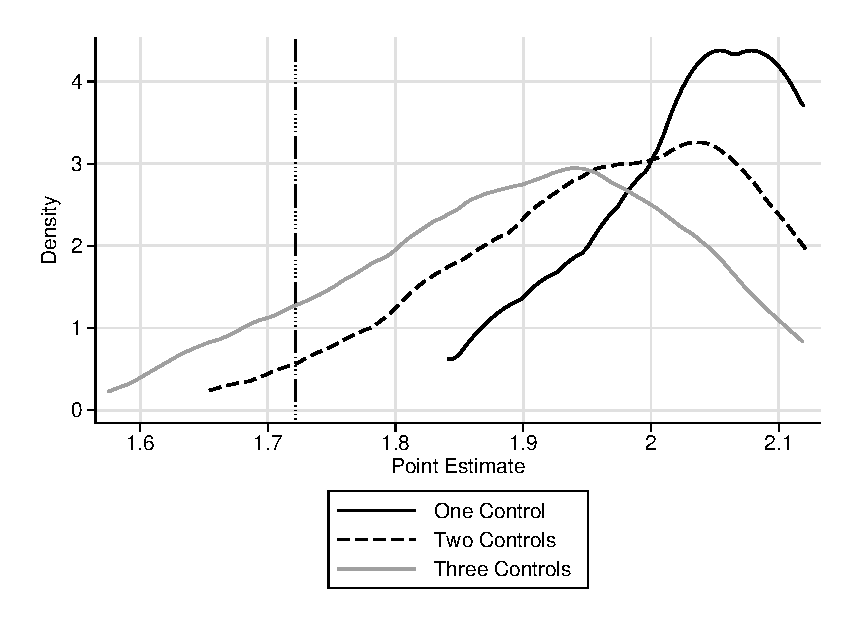
\includegraphics[width=\textwidth]{output/sencontrols_female_years_30y_itt_wctrl.eps}
\end{subfigure}%
\begin{subfigure}[h]{0.4\textwidth}
	\centering
	\caption{Employment, Females}
		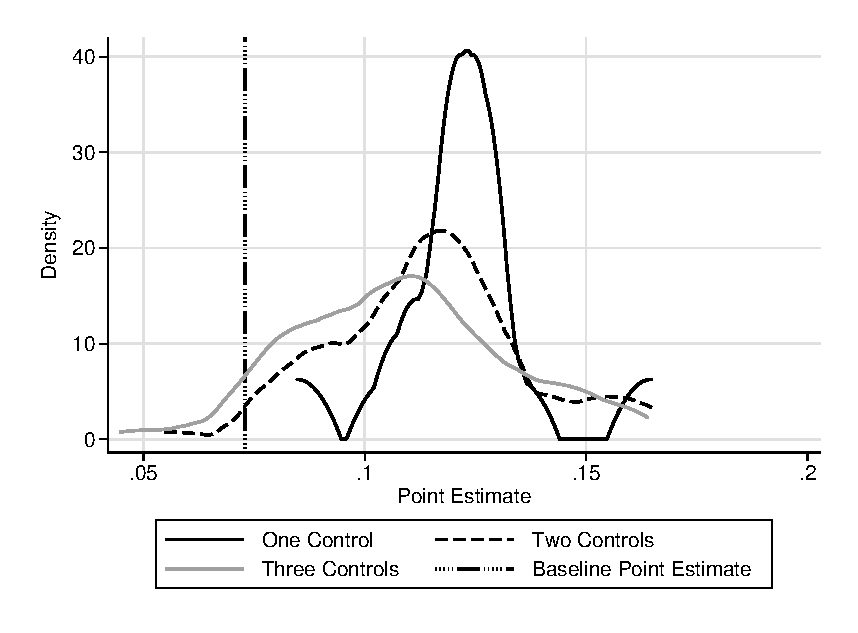
\includegraphics[width=\textwidth]{output/sencontrols_female_si30y_works_itt_wctrl.eps}
\end{subfigure}
\footnotesize \justify
Note: Panel (a) displays the distribution of the treatment effect estimate of the treatment compared to next best counterfactual for males years of education. The distribution is obtained by using all possible combinations of one, two, and three background variables listed in Table~\ref{tab:pselectvars}. In addition to these three variables, we account for a male indicator when computing estimates pooling males and females and a ABC/CARE indicator, to account for any difference in the programs---although we extensively document throughout the paper the similarities between them. The horizontal line marks the baseline estimate we use. The reminder panels present analogous distributions for the outcomes and genders indicated in the title.\\
\end{sidewaysfigure}

\begin{sidewaysfigure}[!htbp]
\centering
\caption{Sensitiviy to Choice of Control Set, Treatment vs. Stay at Home}
\begin{subfigure}[h]{0.4\textwidth}
		\centering
		\caption{Years of Education, Males}
		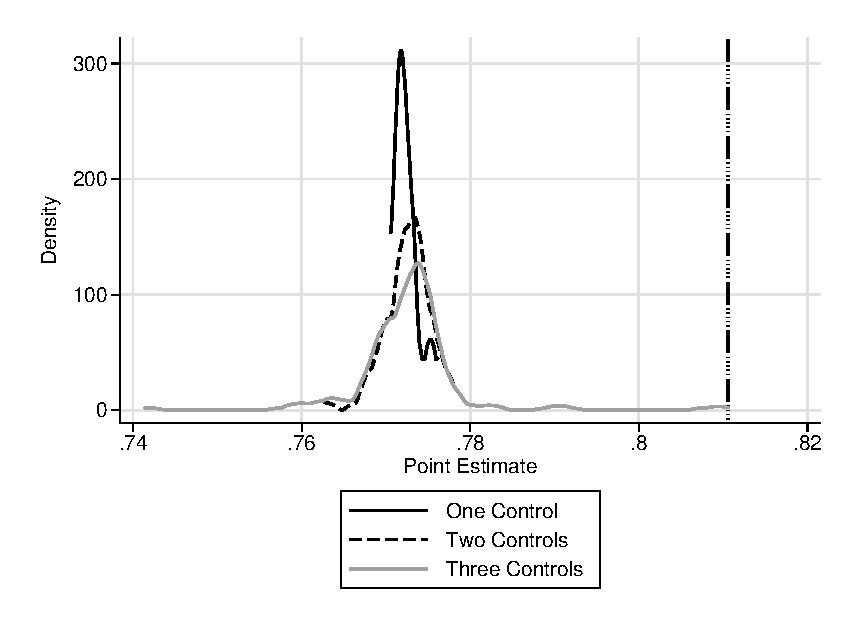
\includegraphics[width=\textwidth]{output/sencontrols_male_years_30y_epan_ipw_P0.eps}
\end{subfigure}%
\begin{subfigure}[h]{0.4\textwidth}
	\centering
	\caption{Employment, Males}
		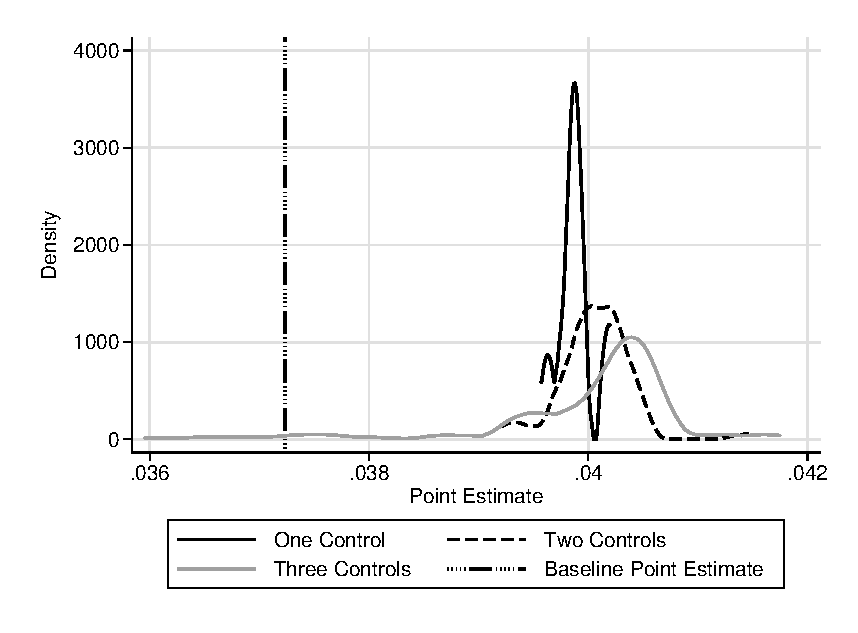
\includegraphics[width=\textwidth]{output/sencontrols_male_si30y_works_epan_ipw_P0.eps}
\end{subfigure}
\begin{subfigure}[h]{0.4\textwidth}
		\centering
		\caption{Years of Education, Females}
		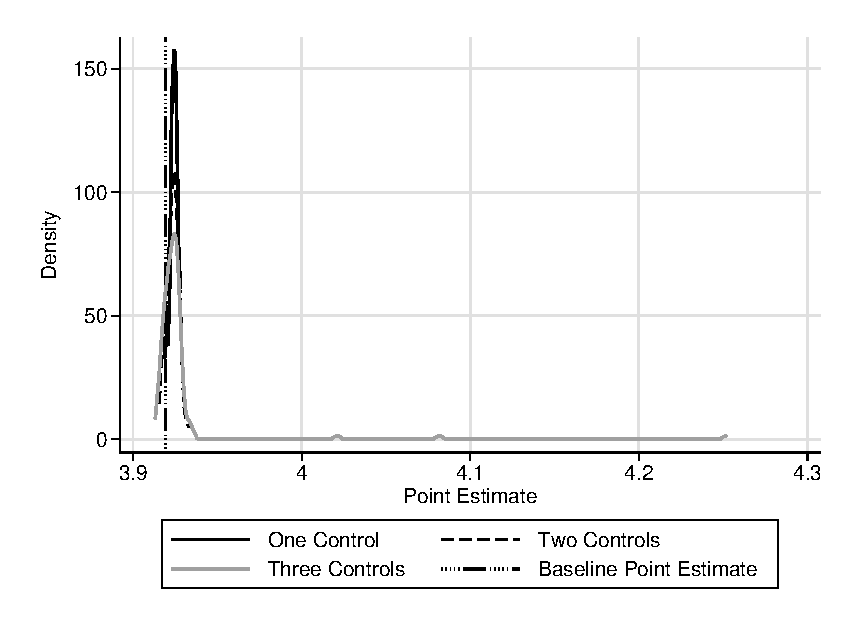
\includegraphics[width=\textwidth]{output/sencontrols_female_years_30y_epan_ipw_P0.eps}
\end{subfigure}%
\begin{subfigure}[h]{0.4\textwidth}
	\centering
	\caption{Employment, Females}
		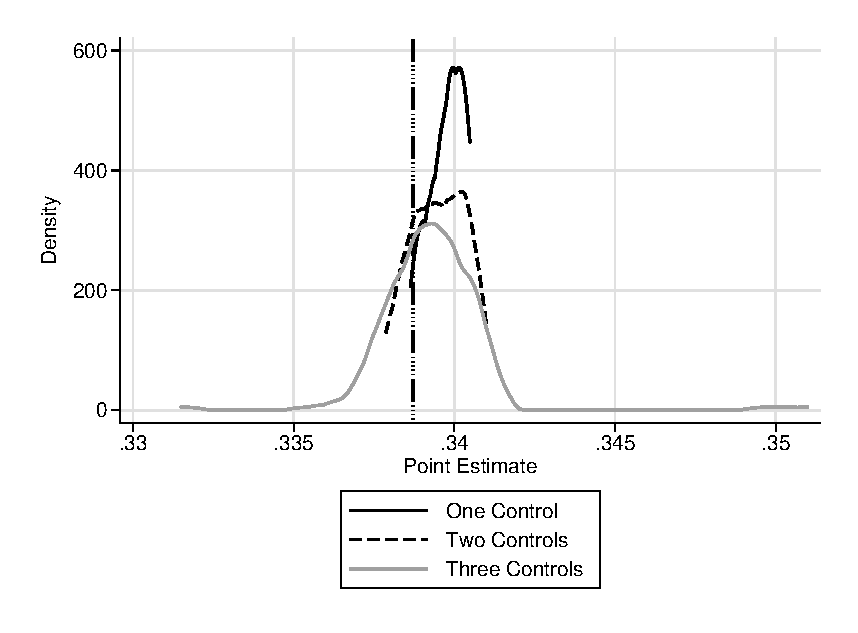
\includegraphics[width=\textwidth]{output/sencontrols_female_si30y_works_epan_ipw_P0.eps}
\end{subfigure}
\footnotesize \justify
Note: Panel (a) displays the distribution of the treatment effect estimate of the treatment compared to stay at home counterfactual for males years of education. The distribution is obtained by using all possible combinations of one, two, and three background variables listed in Table~\ref{tab:pselectvars}. In addition to these three variables, we account for a male indicator when computing estimates pooling males and females and a ABC/CARE indicator, to account for any difference in the programs---although we extensively document throughout the paper the similarities between them. We ``match'' and ``control'' using the same set of variables. The horizontal line marks the baseline estimate we use. The reminder panels present analogous distributions for the outcomes and genders indicated in the title.\\
\end{sidewaysfigure}

\begin{sidewaysfigure}[!htbp]
\centering
\caption{Sensitiviy to Choice of Control Set, Treatment vs. Alternative Preschool}\label{fig:senstap}
\begin{subfigure}[h]{0.4\textwidth}
		\centering
		\caption{Years of Education, Males}
		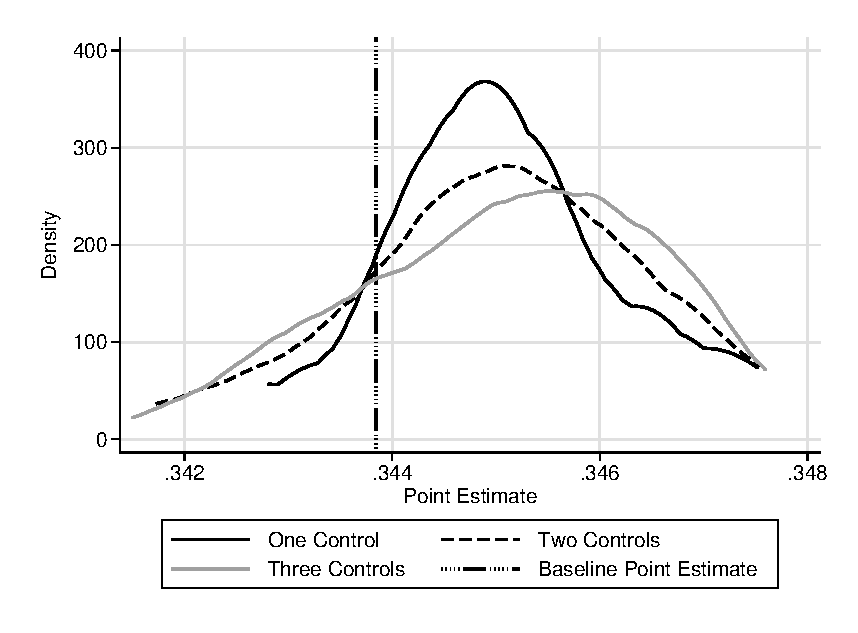
\includegraphics[width=\textwidth]{output/sencontrols_male_years_30y_epan_ipw_P1.eps}
\end{subfigure}%
\begin{subfigure}[h]{0.4\textwidth}
	\centering
	\caption{Employment, Males}
		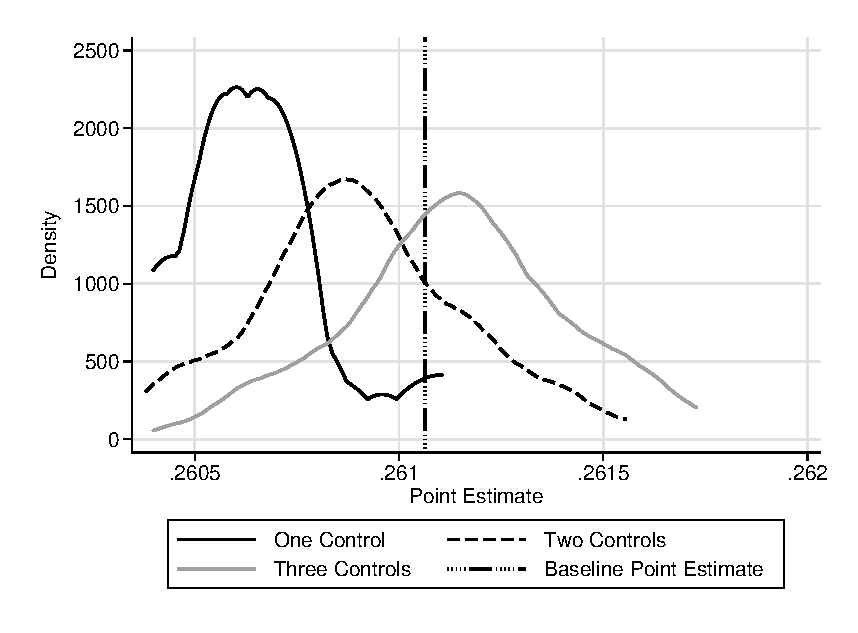
\includegraphics[width=\textwidth]{output/sencontrols_male_si30y_works_epan_ipw_P1.eps}
\end{subfigure}
\begin{subfigure}[h]{0.4\textwidth}
		\centering
		\caption{Years of Education, Females}
		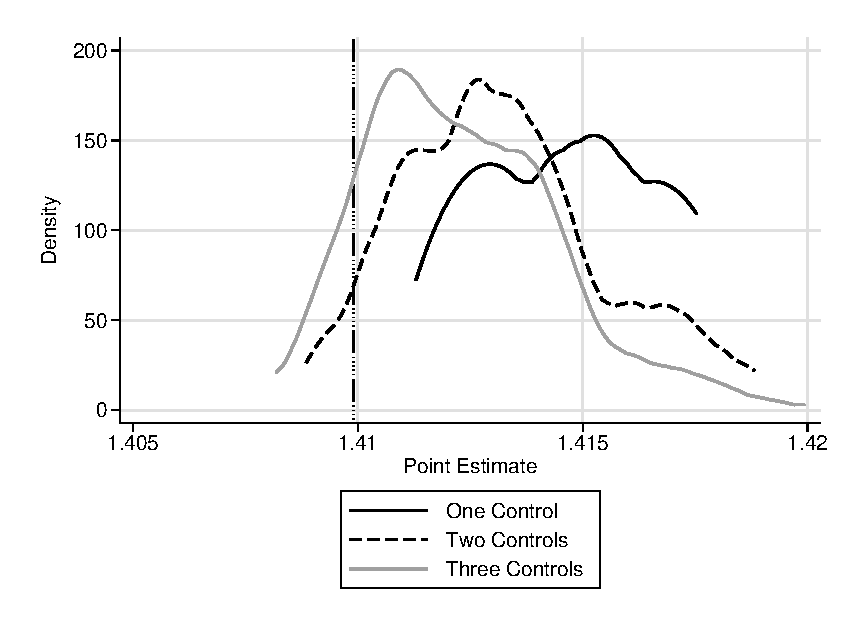
\includegraphics[width=\textwidth]{output/sencontrols_female_years_30y_epan_ipw_P1.eps}
\end{subfigure}%
\begin{subfigure}[h]{0.4\textwidth}
	\centering
	\caption{Employment, Females}
		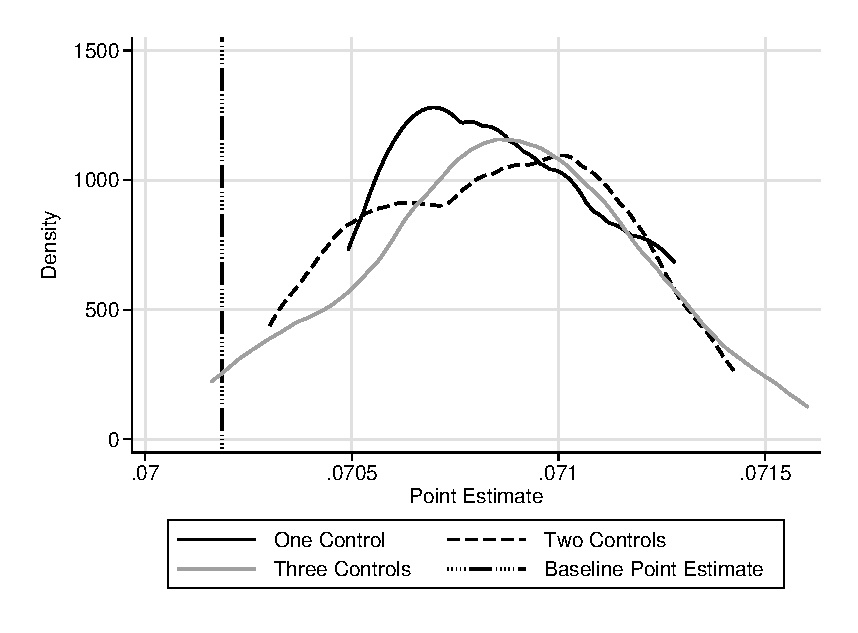
\includegraphics[width=\textwidth]{output/sencontrols_female_si30y_works_epan_ipw_P1.eps}
\end{subfigure}
\footnotesize \justify
Note: Panel (a) displays the distribution of the treatment effect estimate of the treatment compared to alternative preschool counterfactual for males years of education. The distribution is obtained by using all possible combinations of one, two, and three background variables listed in Table~\ref{tab:pselectvars}. In addition to these three variables, we account for a male indicator when computing estimates pooling males and females and a ABC/CARE indicator, to account for any difference in the programs---although we extensively document throughout the paper the similarities between them. We ``match'' and ``control'' using the same set of variables. The horizontal line marks the baseline estimate we use. The reminder panels present analogous distributions for the outcomes and genders indicated in the title.\\
\end{sidewaysfigure}

\subsection{Outcomes of Interest}

\noindent Table \ref{tab:main-outcomes} lists the 95 main outcomes that we test in our main analysis. We reverse the outcomes for which we consider a negative treatment effect socially positive. \\

\singlespacing
\begin{center}
\begin{ThreePartTable}

\begin{TableNotes}[para,flushleft]
Note: This table lists the outcomes that we test treatment effects for. We reverse the outcomes for which we consider a negative treatment effect socially positive.
\end{TableNotes}


\begin{longtable}{L{4cm} L{5cm} C{1cm} C{1cm} C{1.2cm} C{1.5cm}}

\caption{Outcome Variables} \\

\toprule
Category	&	Variable	&	Age	&	ABC	&	CARE	&	Reversed	\\ \midrule
\endfirsthead

\toprule
Category	&	Variable	&	Age	&	ABC	&	CARE	&	Reversed	\\ \midrule
\endhead

\midrule
\endfoot

%\bottomrule
\endlastfoot

IQ Scores	&	Std. IQ Test	&	2	&	\checkmark	&	\checkmark	&		\\
	&		&	2.5	&		&	\checkmark	&		\\
	&		&	3	&	\checkmark	&	\checkmark	&		\\
	&		&	3.5	&	\checkmark	&	\checkmark	&		\\
	&		&	4	&	\checkmark	&	\checkmark	&		\\
	&		&	4.5	&	\checkmark	&	\checkmark	&		\\
	&		&	5	&	\checkmark	&	\checkmark	&		\\
	&		&	6.6	&	\checkmark	&	\checkmark	&		\\
	&		&	7	&	\checkmark	&	\checkmark	&		\\
	&		&	8	&	\checkmark	&	\checkmark	&		\\
	&		&	12	&	\checkmark	&	\checkmark	&		\\
	&		&	15	&	\checkmark	&		&		\\
	&		&	21	&	\checkmark	&		&		\\
	&	IQ Factor	&	2 to 5	&	\checkmark	&	\checkmark	&		\\
	&		&	6 to 12	&	\checkmark	&	\checkmark	&		\\
	&		&	15 to 21	&	\checkmark	&		&		\\     
\\[0.1cm]
Achievement Scores	&	Std. Achv.  Test	&	5.5	&	\checkmark	&	\checkmark	&		\\
	&		&	6	&	\checkmark	&	\checkmark	&		\\
	&		&	6.5	&	\checkmark	&		&		\\
	&		&	7	&	\checkmark	&		&		\\
	&		&	7.5	&	\checkmark	&	\checkmark	&		\\
	&		&	8	&	\checkmark	&	\checkmark	&		\\
	&		&	8.5	&	\checkmark	&	\checkmark	&		\\
	&		&	12	&		&	\checkmark	&		\\
	&		&	15	&	\checkmark	&		&		\\
	&		&	21	&	\checkmark	&		&		\\
	&	PIAT Math Std. Score	&	7	&	\checkmark	&	\checkmark	&		\\
	&	Achievement Factor	&	5.5 to 12	&	\checkmark	&	\checkmark	&		\\
	&		&	15 to 21	&	\checkmark	&		&		\\
\\[0.1cm]
HOME Scores	&	HOME Score	&	0.5	&	\checkmark	&	\checkmark	&		\\
	&		&	1.5	&	\checkmark	&	\checkmark	&		\\
	&		&	2.5	&	\checkmark	&	\checkmark	&		\\
	&		&	3.5	&	\checkmark	&	\checkmark	&		\\
	&		&	4.5	&	\checkmark	&	\checkmark	&		\\
	&		&	8	&	\checkmark	&	\checkmark	&		\\
	&	HOME Factor	&	0.5 to 8	&	\checkmark	&	\checkmark	&		\\
\\[0.1cm]
Parent Income	&	Parental income	&	1.5	&	\checkmark	&	\checkmark	&		\\
	&		&	2.5	&	\checkmark	&	\checkmark	&		\\
	&		&	3.5	&	\checkmark	&	\checkmark	&		\\
	&		&	4.5	&	\checkmark	&	\checkmark	&		\\
	&		&	8	&	\checkmark	&		&		\\
	&		&	12	&	\checkmark	&		&		\\
	&		&	15	&	\checkmark	&		&		\\
	&	Parental Income Factor	&	1.5 to 15	&	\checkmark	&	\checkmark	&		\\
\\[0.1cm]
Mother's Employment	&	Mother Works	&	2	&	\checkmark	&	\checkmark	&		\\
	&		&	3	&	\checkmark	&	\checkmark	&		\\
	&		&	4	&	\checkmark	&	\checkmark	&		\\
	&		&	5	&	\checkmark	&	\checkmark	&		\\
	&		&	21	&	\checkmark	&		&		\\
	&	Mother Works Factor	&	2 to 21	&	\checkmark	&	\checkmark	&		\\
\\[0.1cm]
Mother's Education	&	Mother's Years of Edu.	&	2	&	\checkmark	&		&		\\
	&		&	3	&	\checkmark	&		&		\\
	&		&	4	&	\checkmark	&		&		\\
	&		&	5	&	\checkmark	&		&		\\
	&		&	9	&	\checkmark	&		&		\\
	&	Mother's Edu. Factor	&	2 to 9	&	\checkmark	&		&		\\
\\[0.1cm]
Father at Home	&	Father at Home	&	2	&	\checkmark	&	\checkmark	&		\\
	&		&	3	&	\checkmark	&	\checkmark	&		\\
	&		&	4	&	\checkmark	&	\checkmark	&		\\
	&		&	5	&	\checkmark	&	\checkmark	&		\\
	&		&	8	&	\checkmark	&	\checkmark	&		\\
	&	Father at Home Factor	&	2 to 8	&	\checkmark	&	\checkmark	&		\\
\\[0.1cm]
Adoption	&	Ever Adopted	&	       	&	\checkmark	&		&		\\
\\[0.1cm]
Education	&	Graduated High School	&	30	&	\checkmark	&	\checkmark	&		\\
	&	Attended Voc./Tech./Com. College	&	30	&	\checkmark	&	\checkmark	&		\\
	&	Graduated 4-year College	&	30	&	\checkmark	&	\checkmark	&		\\
	&	Years of Edu.	&	30	&	\checkmark	&	\checkmark	&		\\
	&	Education Factor	&	30	&	\checkmark	&	\checkmark	&		\\
\\[0.1cm]
Employment and Income	&	Employed	&	30	&	\checkmark	&	\checkmark	&		\\
	&	Labor Income	&	21	&	\checkmark	&	\checkmark	&		\\
	&		&	30	&	\checkmark	&	\checkmark	&		\\
	&	Public-Transfer Income	&	21	&	\checkmark	&	\checkmark	&	\checkmark	\\
	&		&	30	&	\checkmark	&	\checkmark	&	\checkmark	\\
	&	Employment Factor	&	21 to 30	&	\checkmark	&	\checkmark	&		\\
\\[0.1cm]
Crime	&	Total Felony Arrests	&	Mid-30s	&	\checkmark	&	\checkmark	&	\checkmark	\\
	&	Total Misdemeanor Arrests	&	Mid-30s	&	\checkmark	&	\checkmark	&	\checkmark	\\
	&	Total Years Incarcerated	&	30	&	\checkmark	&	\checkmark	&	\checkmark	\\
	&	Crime Factor	&	30 to Mid-30s	&	\checkmark	&	\checkmark	&	\checkmark	\\
\\[0.1cm]
Tobacco, Drugs, Alcohol	&	Cig. Smoked per day last month	&	30	&	\checkmark	&	\checkmark	&	\checkmark	\\
	&	Days drank alcohol last month	&	30	&	\checkmark	&	\checkmark	&	\checkmark	\\
	&	Days binge drank alcohol last month	&	30	&	\checkmark	&	\checkmark	&	\checkmark	\\
	&	Self-reported drug user	&	Mid-30s	&	\checkmark	&	\checkmark	&	\checkmark	\\
	&	Substance Use Factor	&	30 to Mid-30s	&	\checkmark	&	\checkmark	&	\checkmark	\\
\\[0.1cm]
Self-Reported Health	&	Self-reported Health	&	30	&	\checkmark	&	\checkmark	&	\checkmark	\\
	&		&	Mid-30s	&	\checkmark	&	\checkmark	&	\checkmark	\\
	&	Self-reported Health Factor	&	30 to Mid-30s	&	\checkmark	&	\checkmark	&	\checkmark	\\
\\[0.1cm]
Hypertension	&	Systolic Blood Pressure (mm Hg)	&	Mid-30s	&	\checkmark	&	\checkmark	&	\checkmark	\\
	&	Diastolic Blood Pressure (mm Hg)	&	Mid-30s	&	\checkmark	&	\checkmark	&	\checkmark	\\
	&	Prehypertension	&	Mid-30s	&	\checkmark	&	\checkmark	&	\checkmark	\\
	&	Hypertension	&	Mid-30s	&	\checkmark	&	\checkmark	&	\checkmark	\\
	&	Hypertension Factor	&	Mid-30s	&	\checkmark	&	\checkmark	&	\checkmark	\\
\\[0.1cm]
Cholesterol	&	High-Density Lipoprotein Chol. (mg/dL)	&	Mid-30s	&	\checkmark	&	\checkmark	&		\\
	&	Dyslipidemia	&	Mid-30s	&	\checkmark	&	\checkmark	&	\checkmark	\\
	&	Cholesterol Factor	&	Mid-30s	&	\checkmark	&	\checkmark	&	\checkmark	\\
\\[0.1cm]
Diabetes	&	Hemoglobin Level (\%)	&	Mid-30s	&	\checkmark	&	\checkmark	&	\checkmark	\\
	&	Prediabetes	&	Mid-30s	&	\checkmark	&	\checkmark	&	\checkmark	\\
	&	Diabetes	&	Mid-30s	&	\checkmark	&	\checkmark	&	\checkmark	\\
	&	Diabetes Factor	&	Mid-30s	&	\checkmark	&	\checkmark	&	\checkmark	\\
\\[0.1cm]
Vitamin D Deficiency	&	Vitamin D Deficiency	&	Mid-30s	&	\checkmark	&	\checkmark	&	\checkmark	\\
\\[0.1cm]
Obesity	&	Measured BMI	&	Mid-30s	&	\checkmark	&	\checkmark	&	\checkmark	\\
	&	Obesity	&	Mid-30s	&	\checkmark	&	\checkmark	&	\checkmark	\\
	&	Severe Obesity	&	Mid-30s	&	\checkmark	&	\checkmark	&	\checkmark	\\
	&	Waist-hip Ratio	&	Mid-30s	&	\checkmark	&	\checkmark	&	\checkmark	\\
	&	Abdominal Obesity	&	Mid-30s	&	\checkmark	&	\checkmark	&	\checkmark	\\
	&	Framingham Risk Score	&	Mid-30s	&	\checkmark	&	\checkmark	&	\checkmark	\\
	&	Obesity Factor	&	Mid-30s	&	\checkmark	&	\checkmark	&	\checkmark	\\
\\[0.1cm]
Mental Health (BSI)	&	Somatization	&	21	&	\checkmark	&	\checkmark	&	\checkmark	\\
	&		&	34	&	\checkmark	&	\checkmark	&	\checkmark	\\
	&	Depression	&	21	&	\checkmark	&	\checkmark	&	\checkmark	\\
	&		&	34	&	\checkmark	&	\checkmark	&	\checkmark	\\
	&	Anxiety	&	21	&	\checkmark	&	\checkmark	&	\checkmark	\\
	&		&	34	&	\checkmark	&	\checkmark	&	\checkmark	\\
	&	Hostility	&	21	&	\checkmark	&	\checkmark	&	\checkmark	\\
	&		&	34	&	\checkmark	&	\checkmark	&	\checkmark	\\
	&	Global Severity Index	&	21	&	\checkmark	&	\checkmark	&	\checkmark	\\
	&		&	34	&	\checkmark	&	\checkmark	&	\checkmark	\\
	&	Mental Health Factor	&	21 and 34	&	\checkmark	&	\checkmark	&	\checkmark	\\
\\[0.1cm]
Child Behavior (CAS)	&	Participates in Activity	&	12	&	\checkmark	&		&		\\
	&	Time Spent Reading	&	12	&	\checkmark	&		&		\\
	&	Good Description of Self	&	12	&	\checkmark	&		&		\\
	&	Views Self as Dumb	&	12	&	\checkmark	&		&	\checkmark	\\
	&	Views Self as Clumsy	&	12	&	\checkmark	&		&	\checkmark	\\
	&	Views Self as Not Liked	&	12	&	\checkmark	&		&	\checkmark	\\
	&	Proud About Self	&	12	&	\checkmark	&		&		\\
	&	Family Proud of You	&	12	&	\checkmark	&		&		\\
	&	Feels Inadequate, Inferior	&	12	&	\checkmark	&		&	\checkmark	\\
	&	Withdraws Excessively	&	12	&	\checkmark	&		&	\checkmark	\\
	&	Ignores Situation	&	12	&	\checkmark	&		&	\checkmark	\\
	&	Not Cope with Prob.	&	12	&	\checkmark	&		&	\checkmark	\\
	&	Often Mad of Angry	&	12	&	\checkmark	&		&	\checkmark	\\
	&	Impulsivity	&	12	&	\checkmark	&		&	\checkmark	\\
	&	Significant Fears	&	12	&	\checkmark	&		&	\checkmark	\\
	&	Denies Any Worries	&	12	&	\checkmark	&		&	\checkmark	\\

\bottomrule
	
\insertTableNotes
\end{longtable}
\end{ThreePartTable}
\end{center}




\doublespacing

\subsection{Estimates} \label{appendix:estimates}

\noindent Table~\ref{table:abccare_rslt_pooled_counts} shows that across all methods of estimation, pooling males and females, over 70\% of the treatment effect estimates are beneficial. When using a 10\% statistical significance level, almost 40\% of all estimates are beneficial. These statistics allow us to reject the hypothesis that there are no treatment effects. \\

\noindent For both males and females, we find positive effects in IQ test scores, achievement test scores, as well as educational attainment. Males also enjoy additional benefits in the areas of employment, labor earnings, and hypertension. \\

\noindent In each of the tables for combining functions and treatment effect estimates, we present 8 different estimates. Column (1) corresponds to the mean difference between the groups randomly assigned to receive center-based childcare and the groups randomly assigned not to. Column (2) adjusts the estimates in (1) for attrition and controls for a set of covariates. Column (3) corresponds to the mean difference between the groups randomly assigned to receive center-based childcare and the groups randomly assigned not to, restricting the latter to subjects who did not receive preschool alternatives. Column (4) adjusts the estimates in (3) for attrition and controls for a set of covariates. Column (5) corresponds to the mean difference between the groups randomly assigned to receive center-based childcare and the groups randomly assigned not to, placing a relatively high weight on the subjects who are likely not to be enrolled in alternative preschools. Column (6) corresponds to the mean difference between the groups randomly assigned to receive center-based childcare and the groups randomly assigned not to, restricting the latter to subjects who received preschool alternatives. Column (7) adjusts the estimates in (6) for attrition and controls for a set of covariates. Column (8) corresponds to the mean difference between the groups randomly assigned to receive center-based childcare and the groups randomly assigned not to, placing a relatively high weight on the children who are likely to be enrolled in alternative preschools. The results in bold are statistically significant at the 10\% level in a single-sided, non-parametric, bootstrapped test.\footnote{For the tables that present categorical combining function statistics that count the number of positive treatment effects that are significant at the 10\% level, two bootstrap tests are conducted. The first bootstrap test is used to determine significance at the 10\% level for each treatment effect. The second bootstrap test is used to determine whether the combined function statistic is significantly different from 10\% at the  10\% level. See Appendix~\ref{appendix:bootstrap} for more details on our inference procedures.} Columns (5) and (8) are standard kernel matching estimates. \\

\noindent Beginning with Table~\ref{table:abccare_rslt_pooled_cat0}, we display treatment effects by outcome. We divide the tables by different blocks of related outcomes. In each table we also present one or two factors constructed with the methodology in Appendix~\ref{app:endogeneity}. The idea behind doing this is to recover a ``latent'' outcome summarizing the outcomes in the table (e.g., latent IQ across IQ from ages 2 to 5). That is, measure the latent outcome using outcomes at various ages as measures of this latent. Testing for treatment effects on this factor it is yet another alternative to summarize treatment effects across a block of outcomes. Table~\ref{table:treatfactors} summarizes treatment effects on the set of selected``latent'' outcomes that we estimate. We display the full set of estimates beginning with Table~\ref{table:abccare_rslt_pooled_cat0}, together with the corresponding outcomes underlying the latents that we estimate.

\begin{table}[H]
\centering
\begin{threeparttable}
\caption{Treatment Effects on Selected Latent Outcomes}\label{table:treatfactors}
\begin{scriptsize}
  \begin{tabular}{cccccccccc}
  \toprule
   Category & Age & (1) & (2) & (3) & (4) & (5) & (6) \\

    \midrule
     \multicolumn{8}{c}{\textbf{\emph{Females}}} \\
    %cat 3
   \mc{1}{l}{\small{Parental Income Latent}} & \mc{1}{c}{\small{1.5 to 21}} & \mc{1}{c}{\small{0.286}} & \mc{1}{c}{\small{0.195}} & \mc{1}{c}{\small{0.578}} & \mc{1}{c}{\small{0.635}} & \mc{1}{c}{\small{0.226}} & \mc{1}{c}{\small{0.297}} \\  

     &  & \mc{1}{c}{\small{\textbf{(0.021)}}} & \mc{1}{c}{\small{\textbf{(0.037)}}} & \mc{1}{c}{\small{\textbf{(0.080)}}} & \mc{1}{c}{\small{(0.143)}} & \mc{1}{c}{\small{\textbf{(0.030)}}} & \mc{1}{c}{\small{(0.197)}} \\  

    \mc{1}{l}{\small{Education Latent}} & \mc{1}{c}{\small{21 to 30}} & \mc{1}{c}{\small{0.561}} & \mc{1}{c}{\small{0.499}} & \mc{1}{c}{\small{0.632}} & \mc{1}{c}{\small{0.726}} & \mc{1}{c}{\small{0.431}} & \mc{1}{c}{\small{0.312}} \\  

     &  & \mc{1}{c}{\small{\textbf{(0.004)}}} & \mc{1}{c}{\small{\textbf{(0.005)}}} & \mc{1}{c}{\small{\textbf{(0.010)}}} & \mc{1}{c}{\small{\textbf{(0.028)}}} & \mc{1}{c}{\small{\textbf{(0.012)}}} & \mc{1}{c}{\small{(0.195)}} \\  

    \mc{1}{l}{\small{Employment Latent}} & \mc{1}{c}{\small{21 to 30}} & \mc{1}{c}{\small{0.434}} & \mc{1}{c}{\small{0.064}} & \mc{1}{c}{\small{0.793}} & \mc{1}{c}{\small{0.998}} & \mc{1}{c}{\small{-0.064}} & \mc{1}{c}{\small{0.244}} \\  

     &  & \mc{1}{c}{\small{\textbf{(0.010)}}} & \mc{1}{c}{\small{\textbf{(0.041)}}} & \mc{1}{c}{\small{\textbf{(0.013)}}} & \mc{1}{c}{\small{\textbf{(0.031)}}} & \mc{1}{c}{\small{\textbf{(0.064)}}} & \mc{1}{c}{\small{(0.233)}} \\  

    \mc{1}{l}{\small{Crime Latent}} & \mc{1}{c}{\small{30 to Mid-30s}} & \mc{1}{c}{\small{-0.239}} & \mc{1}{c}{\small{-0.304}} & \mc{1}{c}{\small{-0.764}} & \mc{1}{c}{\small{-0.725}} & \mc{1}{c}{\small{-0.108}} & \mc{1}{c}{\small{-0.070}} \\  

     &  & \mc{1}{c}{\small{\textbf{(0.009)}}} & \mc{1}{c}{\small{\textbf{(0.008)}}} & \mc{1}{c}{\small{\textbf{(0.010)}}} & \mc{1}{c}{\small{(0.114)}} & \mc{1}{c}{\small{\textbf{(0.020)}}} & \mc{1}{c}{\small{(0.242)}} \\  

    \mc{1}{l}{\small{Hypertension Latent}} & \mc{1}{c}{\small{Mid-30s}} & \mc{1}{c}{\small{-0.061}} & \mc{1}{c}{\small{0.001}} & \mc{1}{c}{\small{0.121}} & \mc{1}{c}{\small{0.178}} & \mc{1}{c}{\small{-0.017}} & \mc{1}{c}{\small{-0.177}} \\  

     &  & \mc{1}{c}{\small{\textbf{(0.042)}}} & \mc{1}{c}{\small{\textbf{(0.051)}}} & \mc{1}{c}{\small{\textbf{(0.063)}}} & \mc{1}{c}{\small{(0.655)}} & \mc{1}{c}{\small{\textbf{(0.049)}}} & \mc{1}{c}{\small{(0.309)}} \\  
     
     
     
     
     
     
     
     
     
     
     
     
     
\midrule     
    \multicolumn{8}{c}{\textbf{\emph{Males}}} \\ 
    %cat 3 

 \mc{1}{l}{\small{Parental Income Latent}} & \mc{1}{c}{\small{1.5 to 21}} & \mc{1}{c}{\small{-0.078}} & \mc{1}{c}{\small{-0.222}} & \mc{1}{c}{\small{1.127}} & \mc{1}{c}{\small{0.363}} & \mc{1}{c}{\small{-0.271}} & \mc{1}{c}{\small{-0.122}} \\  

     &  & \mc{1}{c}{\small{\textbf{(0.057)}}} & \mc{1}{c}{\small{\textbf{(0.077)}}} & \mc{1}{c}{\small{\textbf{(0.094)}}} & \mc{1}{c}{\small{(0.307)}} & \mc{1}{c}{\small{\textbf{(0.079)}}} & \mc{1}{c}{\small{(0.607)}} \\  

    \mc{1}{l}{\small{Education Latent}} & \mc{1}{c}{\small{21 to 30}} & \mc{1}{c}{\small{0.344}} & \mc{1}{c}{\small{0.564}} & \mc{1}{c}{\small{1.020}} & \mc{1}{c}{\small{0.222}} & \mc{1}{c}{\small{0.485}} & \mc{1}{c}{\small{0.375}} \\  

     &  & \mc{1}{c}{\small{\textbf{(0.013)}}} & \mc{1}{c}{\small{\textbf{(0.004)}}} & \mc{1}{c}{\small{\textbf{(0.000)}}} & \mc{1}{c}{\small{(0.299)}} & \mc{1}{c}{\small{\textbf{(0.004)}}} & \mc{1}{c}{\small{\textbf{(0.083)}}} \\  

    \mc{1}{l}{\small{Employment Latent}} & \mc{1}{c}{\small{21 to 30}} & \mc{1}{c}{\small{0.501}} & \mc{1}{c}{\small{0.331}} & \mc{1}{c}{\small{-0.470}} & \mc{1}{c}{\small{0.098}} & \mc{1}{c}{\small{0.517}} & \mc{1}{c}{\small{0.693}} \\  

     &  & \mc{1}{c}{\small{\textbf{(0.007)}}} & \mc{1}{c}{\small{\textbf{(0.019)}}} & \mc{1}{c}{\small{\textbf{(0.001)}}} & \mc{1}{c}{\small{(0.414)}} & \mc{1}{c}{\small{\textbf{(0.012)}}} & \mc{1}{c}{\small{\textbf{(0.065)}}} \\  

    \mc{1}{l}{\small{Crime Latent}} & \mc{1}{c}{\small{30 to Mid-30s}} & \mc{1}{c}{\small{0.192}} & \mc{1}{c}{\small{0.333}} & \mc{1}{c}{\small{0.729}} & \mc{1}{c}{\small{0.648}} & \mc{1}{c}{\small{0.318}} & \mc{1}{c}{\small{0.224}} \\  

     &  & \mc{1}{c}{\small{\textbf{(0.066)}}} & \mc{1}{c}{\small{\textbf{(0.072)}}} & \mc{1}{c}{\small{\textbf{(0.084)}}} & \mc{1}{c}{\small{(0.945)}} & \mc{1}{c}{\small{\textbf{(0.073)}}} & \mc{1}{c}{\small{(0.682)}} \\  

    \mc{1}{l}{\small{Hypertension Latent}} & \mc{1}{c}{\small{Mid-30s}} & \mc{1}{c}{\small{-0.643}} & \mc{1}{c}{\small{-0.920}} & \mc{1}{c}{\small{0.146}} & \mc{1}{c}{\small{-0.025}} & \mc{1}{c}{\small{-1.315}} & \mc{1}{c}{\small{-1.140}} \\  

     &  & \mc{1}{c}{\small{\textbf{(0.004)}}} & \mc{1}{c}{\small{\textbf{(0.002)}}} & \mc{1}{c}{\small{\textbf{(0.097)}}} & \mc{1}{c}{\small{(0.446)}} & \mc{1}{c}{\small{\textbf{(0.000)}}} & \mc{1}{c}{\small{\textbf{(0.002)}}} \\  
     \bottomrule
    \end{tabular} 
\end{scriptsize}
\begin{tablenotes}
\tiny
Note: This table shows the treatment effects for ``latent'' outcomes, constructed from various related outcomes to the latent. We use the method in Appendix~\ref{app:endogeneity} to estimate this latent. Each column present estimates for the following parameters: \textbf{(1)} $\mathbb{E} \big[ \bm{Y}^1 - \bm{Y}^0 | W = 1]$; {\textbf{(2)} $\mathbb{E} \big[ \bm{Y}^1 - \bm{Y}^0 | \bm{B} \big]$}; {\textbf{(3)} $\mathbb{E} \big[ \bm{Y}^1 | \bm{B}, D=1 \big] - \mathbb{E} \big[ \bm{Y}^0 | \bm{B}, V=0, D=0 \big]$}; {\textbf{(4)} $\mathbb{E} \big[ \bm{Y}^1 - \bm{Y}^0 | \bm{B}, V=0 \big] $}; {\textbf{(5)} $\mathbb{E} \big[ \bm{Y}^1 | \bm{B}, D=1 \big] - \mathbb{E} \big[ \bm{Y}^0 | \bm{B}, V=1, D = 0 \big]$}; {\textbf{(6)} $\mathbb{E} \big[ \bm{Y}^1 - \bm{Y}^0 | \bm{B}, V=1 \big]$}. We account for the following background variables ($\bm{B}$): Apgar scores at minutes 1 and 5 and the high-risk index. We define the high-risk index in Appendix~\ref{appendix:background} and explain how we choose the control variables in Appendix~\ref{appendix:bvariables}. Inference is based on non-parametric, one-sided $p$-values from the empirical bootstrap distribution. We highlight point estimates significant at the $10\%$ level.
\end{tablenotes}
\end{threeparttable}
\end{table}
\doublespacing


\def\arraystretch{0.6}

\setlength\tabcolsep{0.3em}

\subsection{{Combining Functions - \% of Positive Treatment Effects, Aggregated}}

\noindent \textbf{[JJH: Document tables!] [We want to test against a null of 1/2 not against zero. Label tables. $p$-values?] [JLG: I have added a footnote for each table. Please see the footnotes. But we are testing the null of 1/2 for beneficial treatment effects and the null of 1/10 for beneficial and significant treatment effects (at 10\%) significance level.]}

	\begin{table}[H]
     \caption{Combining Functions, Pooled Sample} 
     \label{table:abccare_rslt_pooled_counts}
	  \begin{tabular}{ccccccccc}
  \toprule

     & \scriptsize{(1)} & \scriptsize{(2)} & \scriptsize{(3)} & \scriptsize{(4)} & \scriptsize{(5)} & \scriptsize{(6)} & \scriptsize{(7)} & \scriptsize{(8)} \\ 
    \midrule  

    \mc{1}{l}{\scriptsize{\% Pos. TE}} & \mc{1}{c}{\scriptsize{77}} & \mc{1}{c}{\scriptsize{76}} & \mc{1}{c}{\scriptsize{77}} & \mc{1}{c}{\scriptsize{77}} & \mc{1}{c}{\scriptsize{74}} & \mc{1}{c}{\scriptsize{79}} & \mc{1}{c}{\scriptsize{73}} & \mc{1}{c}{\scriptsize{79}} \\  

     & \mc{1}{c}{\scriptsize{\textbf{(0.000)}}} & \mc{1}{c}{\scriptsize{\textbf{(0.000)}}} & \mc{1}{c}{\scriptsize{\textbf{(0.000)}}} & \mc{1}{c}{\scriptsize{\textbf{(0.000)}}} & \mc{1}{c}{\scriptsize{\textbf{(0.000)}}} & \mc{1}{c}{\scriptsize{\textbf{(0.000)}}} & \mc{1}{c}{\scriptsize{\textbf{(0.000)}}} & \mc{1}{c}{\scriptsize{\textbf{(0.000)}}} \\  

    \mc{1}{l}{\scriptsize{\% Pos. TE $|$ 10\% Significance}} & \mc{1}{c}{\scriptsize{53}} & \mc{1}{c}{\scriptsize{47}} & \mc{1}{c}{\scriptsize{38}} & \mc{1}{c}{\scriptsize{34}} & \mc{1}{c}{\scriptsize{39}} & \mc{1}{c}{\scriptsize{46}} & \mc{1}{c}{\scriptsize{41}} & \mc{1}{c}{\scriptsize{44}} \\  

     & \mc{1}{c}{\scriptsize{\textbf{(0.000)}}} & \mc{1}{c}{\scriptsize{\textbf{(0.000)}}} & \mc{1}{c}{\scriptsize{\textbf{(0.000)}}} & \mc{1}{c}{\scriptsize{\textbf{(0.000)}}} & \mc{1}{c}{\scriptsize{\textbf{(0.000)}}} & \mc{1}{c}{\scriptsize{\textbf{(0.000)}}} & \mc{1}{c}{\scriptsize{\textbf{(0.000)}}} & \mc{1}{c}{\scriptsize{\textbf{(0.000)}}} \\  

  \bottomrule
  \end{tabular}
	\end{table}  
\begin{spacing}{1}
\begin{footnotesize}
\noindent 	Note: This table presents estimates of the counts (combining functions) of (i) beneficial treatment effects and (ii) beneficial and significant (at the 10\% level) treatment effects. Counts for the different estimates described in Appendix~\ref{appendix:estimates} are presented in each column. For each count we present a $p$-value underneath. For the counts of beneficial treatment effects, the null hypothesis is that the count is 50\% (half of the treatment effects are positive). For the counts of significant at the 10\% level treatment effects, the null hypotheses is that 10\% of the treatment effects are positive and significant at the 10\% level. 
\end{footnotesize}
\end{spacing}

	\begin{table}[H]
     \caption{Combining Functions, Male Sample} 
     \label{table:abccare_rslt_male_counts}
	  \begin{tabular}{ccccccccc}
  \toprule

     & \scriptsize{(1)} & \scriptsize{(2)} & \scriptsize{(3)} & \scriptsize{(4)} & \scriptsize{(5)} & \scriptsize{(6)} & \scriptsize{(7)} & \scriptsize{(8)} \\ 
    \midrule  

    \mc{1}{l}{\scriptsize{\% Pos. TE}} & \mc{1}{c}{\scriptsize{71}} & \mc{1}{c}{\scriptsize{70}} & \mc{1}{c}{\scriptsize{53}} & \mc{1}{c}{\scriptsize{54}} & \mc{1}{c}{\scriptsize{49}} & \mc{1}{c}{\scriptsize{75}} & \mc{1}{c}{\scriptsize{74}} & \mc{1}{c}{\scriptsize{74}} \\  

     & \mc{1}{c}{\scriptsize{\textbf{(0.000)}}} & \mc{1}{c}{\scriptsize{\textbf{(0.000)}}} & \mc{1}{c}{\scriptsize{(0.347)}} & \mc{1}{c}{\scriptsize{(0.356)}} & \mc{1}{c}{\scriptsize{(0.564)}} & \mc{1}{c}{\scriptsize{\textbf{(0.000)}}} & \mc{1}{c}{\scriptsize{\textbf{(0.000)}}} & \mc{1}{c}{\scriptsize{\textbf{(0.000)}}} \\  

    \mc{1}{l}{\scriptsize{\% Pos. TE $|$ 10\% Significance}} & \mc{1}{c}{\scriptsize{30}} & \mc{1}{c}{\scriptsize{30}} & \mc{1}{c}{\scriptsize{18}} & \mc{1}{c}{\scriptsize{16}} & \mc{1}{c}{\scriptsize{17}} & \mc{1}{c}{\scriptsize{30}} & \mc{1}{c}{\scriptsize{32}} & \mc{1}{c}{\scriptsize{28}} \\  

     & \mc{1}{c}{\scriptsize{\textbf{(0.010)}}} & \mc{1}{c}{\scriptsize{\textbf{(0.000)}}} & \mc{1}{c}{\scriptsize{(0.119)}} & \mc{1}{c}{\scriptsize{(0.208)}} & \mc{1}{c}{\scriptsize{(0.198)}} & \mc{1}{c}{\scriptsize{\textbf{(0.020)}}} & \mc{1}{c}{\scriptsize{\textbf{(0.000)}}} & \mc{1}{c}{\scriptsize{\textbf{(0.030)}}} \\  

  \bottomrule
  \end{tabular}
	\end{table}
\singlespacing
\begin{spacing}{1}
\begin{footnotesize}
\noindent 	Note: This table presents estimates of the counts (combining functions) of (i) beneficial treatment effects and (ii) beneficial and significant (at the 10\% level) treatment effects. Counts for the different estimates described in Appendix~\ref{appendix:estimates} are presented in each column. For each count we present a $p$-value underneath. For the counts of beneficial treatment effects, the null hypothesis is that the count is 50\% (half of the treatment effects are positive). For the counts of significant at the 10\% level treatment effects, the null hypotheses is that 10\% of the treatment effects are positive and significant at the 10\% level. 
\end{footnotesize}
\end{spacing}

	\begin{table}[H]
     \caption{Combining Functions, Female Sample} 
     \label{table:abccare_rslt_female_counts}
	  \begin{tabular}{ccccccccc}
  \toprule

     & \scriptsize{(1)} & \scriptsize{(2)} & \scriptsize{(3)} & \scriptsize{(4)} & \scriptsize{(5)} & \scriptsize{(6)} & \scriptsize{(7)} & \scriptsize{(8)} \\ 
    \midrule  

    \mc{1}{l}{\scriptsize{\% Pos. TE}} & \mc{1}{c}{\scriptsize{83}} & \mc{1}{c}{\scriptsize{77}} & \mc{1}{c}{\scriptsize{78}} & \mc{1}{c}{\scriptsize{79}} & \mc{1}{c}{\scriptsize{79}} & \mc{1}{c}{\scriptsize{82}} & \mc{1}{c}{\scriptsize{67}} & \mc{1}{c}{\scriptsize{79}} \\  

     & \mc{1}{c}{\scriptsize{\textbf{(0.000)}}} & \mc{1}{c}{\scriptsize{\textbf{(0.000)}}} & \mc{1}{c}{\scriptsize{\textbf{(0.000)}}} & \mc{1}{c}{\scriptsize{\textbf{(0.000)}}} & \mc{1}{c}{\scriptsize{\textbf{(0.000)}}} & \mc{1}{c}{\scriptsize{\textbf{(0.000)}}} & \mc{1}{c}{\scriptsize{\textbf{(0.000)}}} & \mc{1}{c}{\scriptsize{\textbf{(0.000)}}} \\  

    \mc{1}{l}{\scriptsize{\% Pos. TE $|$ 10\% Significance}} & \mc{1}{c}{\scriptsize{51}} & \mc{1}{c}{\scriptsize{38}} & \mc{1}{c}{\scriptsize{52}} & \mc{1}{c}{\scriptsize{47}} & \mc{1}{c}{\scriptsize{54}} & \mc{1}{c}{\scriptsize{40}} & \mc{1}{c}{\scriptsize{19}} & \mc{1}{c}{\scriptsize{32}} \\  

     & \mc{1}{c}{\scriptsize{\textbf{(0.000)}}} & \mc{1}{c}{\scriptsize{\textbf{(0.000)}}} & \mc{1}{c}{\scriptsize{\textbf{(0.000)}}} & \mc{1}{c}{\scriptsize{\textbf{(0.000)}}} & \mc{1}{c}{\scriptsize{\textbf{(0.000)}}} & \mc{1}{c}{\scriptsize{\textbf{(0.000)}}} & \mc{1}{c}{\scriptsize{\textbf{(0.069)}}} & \mc{1}{c}{\scriptsize{\textbf{(0.010)}}} \\  

  \bottomrule
  \end{tabular}
	\end{table}  
\begin{spacing}{1}
\begin{footnotesize}
\noindent 	Note: This table presents estimates of the counts (combining functions) of (i) beneficial treatment effects and (ii) beneficial and significant (at the 10\% level) treatment effects. Counts for the different estimates described in Appendix~\ref{appendix:estimates} are presented in each column. For each count we present a $p$-value underneath. For the counts of beneficial treatment effects, the null hypothesis is that the count is 50\% (half of the treatment effects are positive). For the counts of significant at the 10\% level treatment effects, the null hypotheses is that 10\% of the treatment effects are positive and significant at the 10\% level. 
\end{footnotesize}
\end{spacing}
\clearpage

\subsection{{Combining Functions - \% of Positive Treatment Effects, by Category}}


	\begin{table}[H]
     \caption{Combining Functions by Category, Pooled Sample} 
     \label{table:abccare_rslt_pooled_counts_n50a100}
	  \begin{tabular}{cccccccccc}
  \toprule

    \scriptsize{Category} & \scriptsize{(1)} & \scriptsize{(2)} & \scriptsize{(3)} & \scriptsize{(4)} & \scriptsize{(5)} & \scriptsize{(6)} & \scriptsize{(7)} & \scriptsize{(8)} & \scriptsize{N} \\ 
    \midrule  

    \mc{1}{l}{\scriptsize{Cognitive Skills}} & \mc{1}{c}{\scriptsize{93}} & \mc{1}{c}{\scriptsize{93}} & \mc{1}{c}{\scriptsize{93}} & \mc{1}{c}{\scriptsize{90}} & \mc{1}{c}{\scriptsize{93}} & \mc{1}{c}{\scriptsize{90}} & \mc{1}{c}{\scriptsize{93}} & \mc{1}{c}{\scriptsize{93}} & \mc{1}{c}{\scriptsize{29}} \\  

     & \mc{1}{c}{\scriptsize{\textbf{(0.000)}}} & \mc{1}{c}{\scriptsize{\textbf{(0.000)}}} & \mc{1}{c}{\scriptsize{\textbf{(0.000)}}} & \mc{1}{c}{\scriptsize{\textbf{(0.000)}}} & \mc{1}{c}{\scriptsize{\textbf{(0.000)}}} & \mc{1}{c}{\scriptsize{\textbf{(0.000)}}} & \mc{1}{c}{\scriptsize{\textbf{(0.000)}}} & \mc{1}{c}{\scriptsize{\textbf{(0.000)}}} &  \\  

    \mc{1}{l}{\scriptsize{Childhood Household Environment}} & \mc{1}{c}{\scriptsize{62}} & \mc{1}{c}{\scriptsize{69}} & \mc{1}{c}{\scriptsize{54}} & \mc{1}{c}{\scriptsize{54}} & \mc{1}{c}{\scriptsize{54}} & \mc{1}{c}{\scriptsize{85}} & \mc{1}{c}{\scriptsize{62}} & \mc{1}{c}{\scriptsize{92}} & \mc{1}{c}{\scriptsize{13}} \\  

     & \mc{1}{c}{\scriptsize{(0.188)}} & \mc{1}{c}{\scriptsize{(0.248)}} & \mc{1}{c}{\scriptsize{(0.218)}} & \mc{1}{c}{\scriptsize{(0.307)}} & \mc{1}{c}{\scriptsize{(0.158)}} & \mc{1}{c}{\scriptsize{(0.109)}} & \mc{1}{c}{\scriptsize{(0.307)}} & \mc{1}{c}{\scriptsize{\textbf{(0.000)}}} &  \\  

    \mc{1}{l}{\scriptsize{Mother's Employment, Education, and Income}} & \mc{1}{c}{\scriptsize{87}} & \mc{1}{c}{\scriptsize{80}} & \mc{1}{c}{\scriptsize{87}} & \mc{1}{c}{\scriptsize{87}} & \mc{1}{c}{\scriptsize{93}} & \mc{1}{c}{\scriptsize{87}} & \mc{1}{c}{\scriptsize{73}} & \mc{1}{c}{\scriptsize{87}} & \mc{1}{c}{\scriptsize{15}} \\  

     & \mc{1}{c}{\scriptsize{\textbf{(0.000)}}} & \mc{1}{c}{\scriptsize{\textbf{(0.000)}}} & \mc{1}{c}{\scriptsize{\textbf{(0.000)}}} & \mc{1}{c}{\scriptsize{\textbf{(0.000)}}} & \mc{1}{c}{\scriptsize{\textbf{(0.000)}}} & \mc{1}{c}{\scriptsize{\textbf{(0.000)}}} & \mc{1}{c}{\scriptsize{\textbf{(0.000)}}} & \mc{1}{c}{\scriptsize{\textbf{(0.000)}}} &  \\  

    \mc{1}{l}{\scriptsize{Education, Employment, Income}} & \mc{1}{c}{\scriptsize{87}} & \mc{1}{c}{\scriptsize{80}} & \mc{1}{c}{\scriptsize{87}} & \mc{1}{c}{\scriptsize{87}} & \mc{1}{c}{\scriptsize{80}} & \mc{1}{c}{\scriptsize{87}} & \mc{1}{c}{\scriptsize{87}} & \mc{1}{c}{\scriptsize{87}} & \mc{1}{c}{\scriptsize{15}} \\  

     & \mc{1}{c}{\scriptsize{\textbf{(0.000)}}} & \mc{1}{c}{\scriptsize{\textbf{(0.000)}}} & \mc{1}{c}{\scriptsize{\textbf{(0.000)}}} & \mc{1}{c}{\scriptsize{\textbf{(0.000)}}} & \mc{1}{c}{\scriptsize{\textbf{(0.000)}}} & \mc{1}{c}{\scriptsize{\textbf{(0.000)}}} & \mc{1}{c}{\scriptsize{\textbf{(0.000)}}} & \mc{1}{c}{\scriptsize{\textbf{(0.000)}}} &  \\  

    \mc{1}{l}{\scriptsize{Crime}} & \mc{1}{c}{\scriptsize{25}} & \mc{1}{c}{\scriptsize{25}} & \mc{1}{c}{\scriptsize{75}} & \mc{1}{c}{\scriptsize{25}} & \mc{1}{c}{\scriptsize{25}} & \mc{1}{c}{\scriptsize{25}} & \mc{1}{c}{\scriptsize{25}} & \mc{1}{c}{\scriptsize{25}} & \mc{1}{c}{\scriptsize{4}} \\  

     & \mc{1}{c}{\scriptsize{(0.634)}} & \mc{1}{c}{\scriptsize{(0.871)}} & \mc{1}{c}{\scriptsize{\textbf{(0.000)}}} & \mc{1}{c}{\scriptsize{(0.941)}} & \mc{1}{c}{\scriptsize{(0.871)}} & \mc{1}{c}{\scriptsize{(0.960)}} & \mc{1}{c}{\scriptsize{(0.792)}} & \mc{1}{c}{\scriptsize{(0.901)}} &  \\  

    \mc{1}{l}{\scriptsize{Drugs and Alcohol}} & \mc{1}{c}{\scriptsize{20}} & \mc{1}{c}{\scriptsize{20}} & \mc{1}{c}{\scriptsize{80}} & \mc{1}{c}{\scriptsize{80}} & \mc{1}{c}{\scriptsize{60}} & \mc{1}{c}{\scriptsize{20}} & \mc{1}{c}{\scriptsize{20}} & \mc{1}{c}{\scriptsize{20}} & \mc{1}{c}{\scriptsize{5}} \\  

     & \mc{1}{c}{\scriptsize{(0.782)}} & \mc{1}{c}{\scriptsize{(0.990)}} & \mc{1}{c}{\scriptsize{(0.109)}} & \mc{1}{c}{\scriptsize{(0.129)}} & \mc{1}{c}{\scriptsize{(0.297)}} & \mc{1}{c}{\scriptsize{(0.941)}} & \mc{1}{c}{\scriptsize{(0.921)}} & \mc{1}{c}{\scriptsize{(0.921)}} &  \\  

    \mc{1}{l}{\scriptsize{Adult Health}} & \mc{1}{c}{\scriptsize{63}} & \mc{1}{c}{\scriptsize{58}} & \mc{1}{c}{\scriptsize{47}} & \mc{1}{c}{\scriptsize{53}} & \mc{1}{c}{\scriptsize{47}} & \mc{1}{c}{\scriptsize{63}} & \mc{1}{c}{\scriptsize{53}} & \mc{1}{c}{\scriptsize{53}} & \mc{1}{c}{\scriptsize{19}} \\  

     & \mc{1}{c}{\scriptsize{(0.178)}} & \mc{1}{c}{\scriptsize{(0.297)}} & \mc{1}{c}{\scriptsize{(0.634)}} & \mc{1}{c}{\scriptsize{(0.416)}} & \mc{1}{c}{\scriptsize{(0.525)}} & \mc{1}{c}{\scriptsize{(0.238)}} & \mc{1}{c}{\scriptsize{(0.356)}} & \mc{1}{c}{\scriptsize{(0.396)}} &  \\  

    \mc{1}{l}{\scriptsize{Mental Health}} & \mc{1}{c}{\scriptsize{100}} & \mc{1}{c}{\scriptsize{100}} & \mc{1}{c}{\scriptsize{91}} & \mc{1}{c}{\scriptsize{100}} & \mc{1}{c}{\scriptsize{91}} & \mc{1}{c}{\scriptsize{100}} & \mc{1}{c}{\scriptsize{90}} & \mc{1}{c}{\scriptsize{100}} & \mc{1}{c}{\scriptsize{11}} \\  

     & \mc{1}{c}{\scriptsize{\textbf{(0.000)}}} & \mc{1}{c}{\scriptsize{\textbf{(0.000)}}} & \mc{1}{c}{\scriptsize{\textbf{(0.000)}}} & \mc{1}{c}{\scriptsize{\textbf{(0.000)}}} & \mc{1}{c}{\scriptsize{\textbf{(0.000)}}} & \mc{1}{c}{\scriptsize{\textbf{(0.000)}}} & \mc{1}{c}{\scriptsize{\textbf{(0.000)}}} & \mc{1}{c}{\scriptsize{\textbf{(0.000)}}} &  \\  

  \bottomrule
  \end{tabular}
	\end{table}
\begin{spacing}{1}
\begin{footnotesize}
\noindent Note: This table presents estimates of the counts (combining functions) of beneficial treatment effects by the categories of outcomes in each row. The last column presents the number of outcomes per category. Counts for the different estimates described in Appendix~\ref{appendix:estimates} are presented in each column. For each count we present a $p$-value underneath. The null hypothesis is that the count is 50\% (half of the treatment effects are positive).
\end{footnotesize}
\end{spacing}   

	\begin{table}[H]
     \caption{Combining Functions by Category $|$ 10\% Significance, Pooled Sample} 
     \label{table:abccare_rslt_pooled_counts_n10a10}
	  \begin{tabular}{cccccccccc}
  \toprule

    \scriptsize{Category} & \scriptsize{(1)} & \scriptsize{(2)} & \scriptsize{(3)} & \scriptsize{(4)} & \scriptsize{(5)} & \scriptsize{(6)} & \scriptsize{(7)} & \scriptsize{(8)} & \scriptsize{N} \\ 
    \midrule  

    \mc{1}{l}{\scriptsize{Cognitive Skills}} & \mc{1}{c}{\scriptsize{86}} & \mc{1}{c}{\scriptsize{83}} & \mc{1}{c}{\scriptsize{55}} & \mc{1}{c}{\scriptsize{59}} & \mc{1}{c}{\scriptsize{56}} & \mc{1}{c}{\scriptsize{86}} & \mc{1}{c}{\scriptsize{83}} & \mc{1}{c}{\scriptsize{85}} & \mc{1}{c}{\scriptsize{29}} \\  

     & \mc{1}{c}{\scriptsize{\textbf{(0.000)}}} & \mc{1}{c}{\scriptsize{\textbf{(0.000)}}} & \mc{1}{c}{\scriptsize{\textbf{(0.000)}}} & \mc{1}{c}{\scriptsize{\textbf{(0.000)}}} & \mc{1}{c}{\scriptsize{\textbf{(0.000)}}} & \mc{1}{c}{\scriptsize{\textbf{(0.000)}}} & \mc{1}{c}{\scriptsize{\textbf{(0.000)}}} & \mc{1}{c}{\scriptsize{\textbf{(0.000)}}} &  \\  

    \mc{1}{l}{\scriptsize{Childhood Household Environment}} & \mc{1}{c}{\scriptsize{23}} & \mc{1}{c}{\scriptsize{0}} & \mc{1}{c}{\scriptsize{38}} & \mc{1}{c}{\scriptsize{23}} & \mc{1}{c}{\scriptsize{46}} & \mc{1}{c}{\scriptsize{8}} & \mc{1}{c}{\scriptsize{8}} & \mc{1}{c}{\scriptsize{15}} & \mc{1}{c}{\scriptsize{13}} \\  

     & \mc{1}{c}{\scriptsize{(0.198)}} & \mc{1}{c}{\scriptsize{(0.673)}} & \mc{1}{c}{\scriptsize{\textbf{(0.000)}}} & \mc{1}{c}{\scriptsize{(0.257)}} & \mc{1}{c}{\scriptsize{\textbf{(0.000)}}} & \mc{1}{c}{\scriptsize{(0.356)}} & \mc{1}{c}{\scriptsize{(0.416)}} & \mc{1}{c}{\scriptsize{(0.386)}} &  \\  

    \mc{1}{l}{\scriptsize{Mother's Employment, Education, and Income}} & \mc{1}{c}{\scriptsize{53}} & \mc{1}{c}{\scriptsize{40}} & \mc{1}{c}{\scriptsize{53}} & \mc{1}{c}{\scriptsize{40}} & \mc{1}{c}{\scriptsize{47}} & \mc{1}{c}{\scriptsize{27}} & \mc{1}{c}{\scriptsize{27}} & \mc{1}{c}{\scriptsize{33}} & \mc{1}{c}{\scriptsize{15}} \\  

     & \mc{1}{c}{\scriptsize{\textbf{(0.010)}}} & \mc{1}{c}{\scriptsize{\textbf{(0.040)}}} & \mc{1}{c}{\scriptsize{\textbf{(0.000)}}} & \mc{1}{c}{\scriptsize{\textbf{(0.040)}}} & \mc{1}{c}{\scriptsize{\textbf{(0.010)}}} & \mc{1}{c}{\scriptsize{(0.109)}} & \mc{1}{c}{\scriptsize{\textbf{(0.079)}}} & \mc{1}{c}{\scriptsize{\textbf{(0.079)}}} &  \\  

    \mc{1}{l}{\scriptsize{Education, Employment, Income}} & \mc{1}{c}{\scriptsize{67}} & \mc{1}{c}{\scriptsize{60}} & \mc{1}{c}{\scriptsize{40}} & \mc{1}{c}{\scriptsize{40}} & \mc{1}{c}{\scriptsize{53}} & \mc{1}{c}{\scriptsize{60}} & \mc{1}{c}{\scriptsize{47}} & \mc{1}{c}{\scriptsize{53}} & \mc{1}{c}{\scriptsize{15}} \\  

     & \mc{1}{c}{\scriptsize{\textbf{(0.000)}}} & \mc{1}{c}{\scriptsize{\textbf{(0.000)}}} & \mc{1}{c}{\scriptsize{\textbf{(0.020)}}} & \mc{1}{c}{\scriptsize{\textbf{(0.000)}}} & \mc{1}{c}{\scriptsize{\textbf{(0.000)}}} & \mc{1}{c}{\scriptsize{\textbf{(0.000)}}} & \mc{1}{c}{\scriptsize{\textbf{(0.000)}}} & \mc{1}{c}{\scriptsize{\textbf{(0.020)}}} &  \\  

    \mc{1}{l}{\scriptsize{Crime}} & \mc{1}{c}{\scriptsize{25}} & \mc{1}{c}{\scriptsize{0}} & \mc{1}{c}{\scriptsize{0}} & \mc{1}{c}{\scriptsize{0}} & \mc{1}{c}{\scriptsize{0}} & \mc{1}{c}{\scriptsize{25}} & \mc{1}{c}{\scriptsize{0}} & \mc{1}{c}{\scriptsize{0}} & \mc{1}{c}{\scriptsize{4}} \\  

     & \mc{1}{c}{\scriptsize{(0.139)}} & \mc{1}{c}{\scriptsize{(1.000)}} & \mc{1}{c}{\scriptsize{(1.000)}} & \mc{1}{c}{\scriptsize{(1.000)}} & \mc{1}{c}{\scriptsize{(1.000)}} & \mc{1}{c}{\scriptsize{\textbf{(0.079)}}} & \mc{1}{c}{\scriptsize{(1.000)}} & \mc{1}{c}{\scriptsize{(1.000)}} &  \\  

    \mc{1}{l}{\scriptsize{Drugs and Alcohol}} & \mc{1}{c}{\scriptsize{20}} & \mc{1}{c}{\scriptsize{20}} & \mc{1}{c}{\scriptsize{20}} & \mc{1}{c}{\scriptsize{20}} & \mc{1}{c}{\scriptsize{20}} & \mc{1}{c}{\scriptsize{0}} & \mc{1}{c}{\scriptsize{0}} & \mc{1}{c}{\scriptsize{0}} & \mc{1}{c}{\scriptsize{5}} \\  

     & \mc{1}{c}{\scriptsize{\textbf{(0.059)}}} & \mc{1}{c}{\scriptsize{\textbf{(0.020)}}} & \mc{1}{c}{\scriptsize{\textbf{(0.079)}}} & \mc{1}{c}{\scriptsize{(0.119)}} & \mc{1}{c}{\scriptsize{\textbf{(0.059)}}} & \mc{1}{c}{\scriptsize{(1.000)}} & \mc{1}{c}{\scriptsize{(1.000)}} & \mc{1}{c}{\scriptsize{(1.000)}} &  \\  

    \mc{1}{l}{\scriptsize{Adult Health}} & \mc{1}{c}{\scriptsize{21}} & \mc{1}{c}{\scriptsize{26}} & \mc{1}{c}{\scriptsize{16}} & \mc{1}{c}{\scriptsize{0}} & \mc{1}{c}{\scriptsize{11}} & \mc{1}{c}{\scriptsize{26}} & \mc{1}{c}{\scriptsize{26}} & \mc{1}{c}{\scriptsize{21}} & \mc{1}{c}{\scriptsize{19}} \\  

     & \mc{1}{c}{\scriptsize{(0.218)}} & \mc{1}{c}{\scriptsize{\textbf{(0.050)}}} & \mc{1}{c}{\scriptsize{(0.317)}} & \mc{1}{c}{\scriptsize{(1.000)}} & \mc{1}{c}{\scriptsize{(0.406)}} & \mc{1}{c}{\scriptsize{\textbf{(0.040)}}} & \mc{1}{c}{\scriptsize{\textbf{(0.010)}}} & \mc{1}{c}{\scriptsize{\textbf{(0.089)}}} &  \\  

    \mc{1}{l}{\scriptsize{Mental Health}} & \mc{1}{c}{\scriptsize{64}} & \mc{1}{c}{\scriptsize{64}} & \mc{1}{c}{\scriptsize{27}} & \mc{1}{c}{\scriptsize{45}} & \mc{1}{c}{\scriptsize{36}} & \mc{1}{c}{\scriptsize{55}} & \mc{1}{c}{\scriptsize{40}} & \mc{1}{c}{\scriptsize{55}} & \mc{1}{c}{\scriptsize{11}} \\  

     & \mc{1}{c}{\scriptsize{\textbf{(0.010)}}} & \mc{1}{c}{\scriptsize{\textbf{(0.030)}}} & \mc{1}{c}{\scriptsize{(0.228)}} & \mc{1}{c}{\scriptsize{\textbf{(0.010)}}} & \mc{1}{c}{\scriptsize{\textbf{(0.040)}}} & \mc{1}{c}{\scriptsize{\textbf{(0.040)}}} & \mc{1}{c}{\scriptsize{(0.139)}} & \mc{1}{c}{\scriptsize{\textbf{(0.010)}}} &  \\  

  \bottomrule
  \end{tabular}
	\end{table}
\begin{spacing}{1}
\begin{footnotesize}
\noindent Note: This table presents estimates of the counts (combining functions) of beneficial and significant (at the 10\% level) treatment effects by the categories of outcomes in each row. The last column presents the number of outcomes per category. Counts for the different estimates described in Appendix~\ref{appendix:estimates} are presented in each column. For each count we present a $p$-value underneath. The null hypothesis is that 10\% of the treatment effects are positive and significant at the 10\% level.
\end{footnotesize}
\end{spacing}

	\begin{table}[H]
     \caption{Combining Functions by Category, Male Sample} 
     \label{table:abccare_rslt_male_counts_n50a100}
	  \begin{tabular}{cccccccccc}
  \toprule

    \scriptsize{Category} & \scriptsize{(1)} & \scriptsize{(2)} & \scriptsize{(3)} & \scriptsize{(4)} & \scriptsize{(5)} & \scriptsize{(6)} & \scriptsize{(7)} & \scriptsize{(8)} & \scriptsize{N} \\ 
    \midrule  

    \mc{1}{l}{\scriptsize{Cognitive Skills}} & \mc{1}{c}{\scriptsize{90}} & \mc{1}{c}{\scriptsize{83}} & \mc{1}{c}{\scriptsize{69}} & \mc{1}{c}{\scriptsize{76}} & \mc{1}{c}{\scriptsize{63}} & \mc{1}{c}{\scriptsize{90}} & \mc{1}{c}{\scriptsize{86}} & \mc{1}{c}{\scriptsize{81}} & \mc{1}{c}{\scriptsize{29}} \\  

     & \mc{1}{c}{\scriptsize{\textbf{(0.000)}}} & \mc{1}{c}{\scriptsize{\textbf{(0.000)}}} & \mc{1}{c}{\scriptsize{(0.158)}} & \mc{1}{c}{\scriptsize{\textbf{(0.020)}}} & \mc{1}{c}{\scriptsize{(0.248)}} & \mc{1}{c}{\scriptsize{\textbf{(0.000)}}} & \mc{1}{c}{\scriptsize{\textbf{(0.000)}}} & \mc{1}{c}{\scriptsize{\textbf{(0.000)}}} &  \\  

    \mc{1}{l}{\scriptsize{Childhood Household Environment}} & \mc{1}{c}{\scriptsize{54}} & \mc{1}{c}{\scriptsize{62}} & \mc{1}{c}{\scriptsize{46}} & \mc{1}{c}{\scriptsize{46}} & \mc{1}{c}{\scriptsize{46}} & \mc{1}{c}{\scriptsize{75}} & \mc{1}{c}{\scriptsize{77}} & \mc{1}{c}{\scriptsize{85}} & \mc{1}{c}{\scriptsize{13}} \\  

     & \mc{1}{c}{\scriptsize{(0.386)}} & \mc{1}{c}{\scriptsize{(0.337)}} & \mc{1}{c}{\scriptsize{(0.594)}} & \mc{1}{c}{\scriptsize{(0.495)}} & \mc{1}{c}{\scriptsize{(0.594)}} & \mc{1}{c}{\scriptsize{(0.158)}} & \mc{1}{c}{\scriptsize{\textbf{(0.089)}}} & \mc{1}{c}{\scriptsize{\textbf{(0.000)}}} &  \\  

    \mc{1}{l}{\scriptsize{Mother's Employment, Education, and Income}} & \mc{1}{c}{\scriptsize{80}} & \mc{1}{c}{\scriptsize{60}} & \mc{1}{c}{\scriptsize{73}} & \mc{1}{c}{\scriptsize{60}} & \mc{1}{c}{\scriptsize{60}} & \mc{1}{c}{\scriptsize{60}} & \mc{1}{c}{\scriptsize{60}} & \mc{1}{c}{\scriptsize{67}} & \mc{1}{c}{\scriptsize{15}} \\  

     & \mc{1}{c}{\scriptsize{\textbf{(0.000)}}} & \mc{1}{c}{\scriptsize{(0.238)}} & \mc{1}{c}{\scriptsize{\textbf{(0.030)}}} & \mc{1}{c}{\scriptsize{(0.257)}} & \mc{1}{c}{\scriptsize{(0.297)}} & \mc{1}{c}{\scriptsize{(0.446)}} & \mc{1}{c}{\scriptsize{(0.327)}} & \mc{1}{c}{\scriptsize{(0.238)}} &  \\  

    \mc{1}{l}{\scriptsize{Education, Employment, Income}} & \mc{1}{c}{\scriptsize{80}} & \mc{1}{c}{\scriptsize{80}} & \mc{1}{c}{\scriptsize{53}} & \mc{1}{c}{\scriptsize{67}} & \mc{1}{c}{\scriptsize{60}} & \mc{1}{c}{\scriptsize{87}} & \mc{1}{c}{\scriptsize{87}} & \mc{1}{c}{\scriptsize{80}} & \mc{1}{c}{\scriptsize{15}} \\  

     & \mc{1}{c}{\scriptsize{\textbf{(0.000)}}} & \mc{1}{c}{\scriptsize{\textbf{(0.000)}}} & \mc{1}{c}{\scriptsize{(0.426)}} & \mc{1}{c}{\scriptsize{\textbf{(0.089)}}} & \mc{1}{c}{\scriptsize{(0.337)}} & \mc{1}{c}{\scriptsize{\textbf{(0.000)}}} & \mc{1}{c}{\scriptsize{\textbf{(0.000)}}} & \mc{1}{c}{\scriptsize{\textbf{(0.000)}}} &  \\  

    \mc{1}{l}{\scriptsize{Crime}} & \mc{1}{c}{\scriptsize{25}} & \mc{1}{c}{\scriptsize{25}} & \mc{1}{c}{\scriptsize{25}} & \mc{1}{c}{\scriptsize{25}} & \mc{1}{c}{\scriptsize{25}} & \mc{1}{c}{\scriptsize{25}} & \mc{1}{c}{\scriptsize{25}} & \mc{1}{c}{\scriptsize{25}} & \mc{1}{c}{\scriptsize{4}} \\  

     & \mc{1}{c}{\scriptsize{(0.861)}} & \mc{1}{c}{\scriptsize{(0.693)}} & \mc{1}{c}{\scriptsize{(1.000)}} & \mc{1}{c}{\scriptsize{(1.000)}} & \mc{1}{c}{\scriptsize{(1.000)}} & \mc{1}{c}{\scriptsize{(0.891)}} & \mc{1}{c}{\scriptsize{(0.713)}} & \mc{1}{c}{\scriptsize{(0.901)}} &  \\  

    \mc{1}{l}{\scriptsize{Drugs and Alcohol}} & \mc{1}{c}{\scriptsize{20}} & \mc{1}{c}{\scriptsize{20}} & \mc{1}{c}{\scriptsize{40}} & \mc{1}{c}{\scriptsize{60}} & \mc{1}{c}{\scriptsize{20}} & \mc{1}{c}{\scriptsize{20}} & \mc{1}{c}{\scriptsize{20}} & \mc{1}{c}{\scriptsize{20}} & \mc{1}{c}{\scriptsize{5}} \\  

     & \mc{1}{c}{\scriptsize{(1.000)}} & \mc{1}{c}{\scriptsize{(0.990)}} & \mc{1}{c}{\scriptsize{(0.475)}} & \mc{1}{c}{\scriptsize{(0.267)}} & \mc{1}{c}{\scriptsize{(0.921)}} & \mc{1}{c}{\scriptsize{(0.970)}} & \mc{1}{c}{\scriptsize{(0.970)}} & \mc{1}{c}{\scriptsize{(0.960)}} &  \\  

    \mc{1}{l}{\scriptsize{Adult Health}} & \mc{1}{c}{\scriptsize{58}} & \mc{1}{c}{\scriptsize{74}} & \mc{1}{c}{\scriptsize{37}} & \mc{1}{c}{\scriptsize{37}} & \mc{1}{c}{\scriptsize{32}} & \mc{1}{c}{\scriptsize{68}} & \mc{1}{c}{\scriptsize{74}} & \mc{1}{c}{\scriptsize{74}} & \mc{1}{c}{\scriptsize{19}} \\  

     & \mc{1}{c}{\scriptsize{(0.376)}} & \mc{1}{c}{\scriptsize{\textbf{(0.040)}}} & \mc{1}{c}{\scriptsize{(0.713)}} & \mc{1}{c}{\scriptsize{(0.752)}} & \mc{1}{c}{\scriptsize{(0.822)}} & \mc{1}{c}{\scriptsize{\textbf{(0.089)}}} & \mc{1}{c}{\scriptsize{\textbf{(0.050)}}} & \mc{1}{c}{\scriptsize{\textbf{(0.000)}}} &  \\  

    \mc{1}{l}{\scriptsize{Mental Health}} & \mc{1}{c}{\scriptsize{82}} & \mc{1}{c}{\scriptsize{82}} & \mc{1}{c}{\scriptsize{36}} & \mc{1}{c}{\scriptsize{18}} & \mc{1}{c}{\scriptsize{36}} & \mc{1}{c}{\scriptsize{91}} & \mc{1}{c}{\scriptsize{82}} & \mc{1}{c}{\scriptsize{91}} & \mc{1}{c}{\scriptsize{11}} \\  

     & \mc{1}{c}{\scriptsize{\textbf{(0.000)}}} & \mc{1}{c}{\scriptsize{\textbf{(0.000)}}} & \mc{1}{c}{\scriptsize{(0.772)}} & \mc{1}{c}{\scriptsize{(0.931)}} & \mc{1}{c}{\scriptsize{(0.802)}} & \mc{1}{c}{\scriptsize{\textbf{(0.000)}}} & \mc{1}{c}{\scriptsize{\textbf{(0.000)}}} & \mc{1}{c}{\scriptsize{\textbf{(0.000)}}} &  \\  

  \bottomrule
  \end{tabular}
	\end{table}
\begin{spacing}{1}
\begin{footnotesize}
\noindent Note: This table presents estimates of the counts (combining functions) of beneficial treatment effects by the categories of outcomes in each row. The last column presents the number of outcomes per category. Counts for the different estimates described in Appendix~\ref{appendix:estimates} are presented in each column. For each count we present a $p$-value underneath. The null hypothesis is that the count is 50\% (half of the treatment effects are positive).
\end{footnotesize}
\end{spacing}   

	\begin{table}[H]
     \caption{Combining Functions by Category $|$ 10\% Significance, Male Sample} 
     \label{table:abccare_rslt_male_counts_n10a10}
	  \begin{tabular}{cccccccccc}
  \toprule

    \scriptsize{Category} & \scriptsize{(1)} & \scriptsize{(2)} & \scriptsize{(3)} & \scriptsize{(4)} & \scriptsize{(5)} & \scriptsize{(6)} & \scriptsize{(7)} & \scriptsize{(8)} & \scriptsize{N} \\ 
    \midrule  

    \mc{1}{l}{\scriptsize{Cognitive Skills}} & \mc{1}{c}{\scriptsize{55}} & \mc{1}{c}{\scriptsize{59}} & \mc{1}{c}{\scriptsize{21}} & \mc{1}{c}{\scriptsize{21}} & \mc{1}{c}{\scriptsize{26}} & \mc{1}{c}{\scriptsize{59}} & \mc{1}{c}{\scriptsize{69}} & \mc{1}{c}{\scriptsize{56}} & \mc{1}{c}{\scriptsize{29}} \\  

     & \mc{1}{c}{\scriptsize{\textbf{(0.000)}}} & \mc{1}{c}{\scriptsize{\textbf{(0.000)}}} & \mc{1}{c}{\scriptsize{(0.198)}} & \mc{1}{c}{\scriptsize{(0.238)}} & \mc{1}{c}{\scriptsize{(0.168)}} & \mc{1}{c}{\scriptsize{\textbf{(0.000)}}} & \mc{1}{c}{\scriptsize{\textbf{(0.000)}}} & \mc{1}{c}{\scriptsize{\textbf{(0.000)}}} &  \\  

    \mc{1}{l}{\scriptsize{Childhood Household Environment}} & \mc{1}{c}{\scriptsize{0}} & \mc{1}{c}{\scriptsize{0}} & \mc{1}{c}{\scriptsize{0}} & \mc{1}{c}{\scriptsize{23}} & \mc{1}{c}{\scriptsize{0}} & \mc{1}{c}{\scriptsize{8}} & \mc{1}{c}{\scriptsize{0}} & \mc{1}{c}{\scriptsize{8}} & \mc{1}{c}{\scriptsize{13}} \\  

     & \mc{1}{c}{\scriptsize{(1.000)}} & \mc{1}{c}{\scriptsize{(1.000)}} & \mc{1}{c}{\scriptsize{(1.000)}} & \mc{1}{c}{\scriptsize{(0.129)}} & \mc{1}{c}{\scriptsize{(1.000)}} & \mc{1}{c}{\scriptsize{(0.386)}} & \mc{1}{c}{\scriptsize{(0.644)}} & \mc{1}{c}{\scriptsize{(0.337)}} &  \\  

    \mc{1}{l}{\scriptsize{Mother's Employment, Education, and Income}} & \mc{1}{c}{\scriptsize{33}} & \mc{1}{c}{\scriptsize{20}} & \mc{1}{c}{\scriptsize{47}} & \mc{1}{c}{\scriptsize{20}} & \mc{1}{c}{\scriptsize{33}} & \mc{1}{c}{\scriptsize{20}} & \mc{1}{c}{\scriptsize{20}} & \mc{1}{c}{\scriptsize{13}} & \mc{1}{c}{\scriptsize{15}} \\  

     & \mc{1}{c}{\scriptsize{\textbf{(0.040)}}} & \mc{1}{c}{\scriptsize{(0.168)}} & \mc{1}{c}{\scriptsize{\textbf{(0.030)}}} & \mc{1}{c}{\scriptsize{(0.228)}} & \mc{1}{c}{\scriptsize{(0.119)}} & \mc{1}{c}{\scriptsize{(0.198)}} & \mc{1}{c}{\scriptsize{(0.119)}} & \mc{1}{c}{\scriptsize{(0.267)}} &  \\  

    \mc{1}{l}{\scriptsize{Education, Employment, Income}} & \mc{1}{c}{\scriptsize{27}} & \mc{1}{c}{\scriptsize{47}} & \mc{1}{c}{\scriptsize{7}} & \mc{1}{c}{\scriptsize{13}} & \mc{1}{c}{\scriptsize{13}} & \mc{1}{c}{\scriptsize{33}} & \mc{1}{c}{\scriptsize{33}} & \mc{1}{c}{\scriptsize{27}} & \mc{1}{c}{\scriptsize{15}} \\  

     & \mc{1}{c}{\scriptsize{(0.208)}} & \mc{1}{c}{\scriptsize{\textbf{(0.000)}}} & \mc{1}{c}{\scriptsize{(0.525)}} & \mc{1}{c}{\scriptsize{(0.337)}} & \mc{1}{c}{\scriptsize{(0.317)}} & \mc{1}{c}{\scriptsize{\textbf{(0.069)}}} & \mc{1}{c}{\scriptsize{\textbf{(0.020)}}} & \mc{1}{c}{\scriptsize{(0.139)}} &  \\  

    \mc{1}{l}{\scriptsize{Crime}} & \mc{1}{c}{\scriptsize{0}} & \mc{1}{c}{\scriptsize{0}} & \mc{1}{c}{\scriptsize{0}} & \mc{1}{c}{\scriptsize{0}} & \mc{1}{c}{\scriptsize{0}} & \mc{1}{c}{\scriptsize{0}} & \mc{1}{c}{\scriptsize{0}} & \mc{1}{c}{\scriptsize{0}} & \mc{1}{c}{\scriptsize{4}} \\  

     & \mc{1}{c}{\scriptsize{(1.000)}} & \mc{1}{c}{\scriptsize{(1.000)}} & \mc{1}{c}{\scriptsize{(1.000)}} & \mc{1}{c}{\scriptsize{(1.000)}} & \mc{1}{c}{\scriptsize{(1.000)}} & \mc{1}{c}{\scriptsize{(1.000)}} & \mc{1}{c}{\scriptsize{(1.000)}} & \mc{1}{c}{\scriptsize{(1.000)}} &  \\  

    \mc{1}{l}{\scriptsize{Drugs and Alcohol}} & \mc{1}{c}{\scriptsize{20}} & \mc{1}{c}{\scriptsize{20}} & \mc{1}{c}{\scriptsize{0}} & \mc{1}{c}{\scriptsize{20}} & \mc{1}{c}{\scriptsize{20}} & \mc{1}{c}{\scriptsize{0}} & \mc{1}{c}{\scriptsize{20}} & \mc{1}{c}{\scriptsize{20}} & \mc{1}{c}{\scriptsize{5}} \\  

     & \mc{1}{c}{\scriptsize{\textbf{(0.050)}}} & \mc{1}{c}{\scriptsize{\textbf{(0.079)}}} & \mc{1}{c}{\scriptsize{(0.564)}} & \mc{1}{c}{\scriptsize{(0.406)}} & \mc{1}{c}{\scriptsize{\textbf{(0.089)}}} & \mc{1}{c}{\scriptsize{(1.000)}} & \mc{1}{c}{\scriptsize{(0.109)}} & \mc{1}{c}{\scriptsize{\textbf{(0.000)}}} &  \\  

    \mc{1}{l}{\scriptsize{Adult Health}} & \mc{1}{c}{\scriptsize{32}} & \mc{1}{c}{\scriptsize{21}} & \mc{1}{c}{\scriptsize{21}} & \mc{1}{c}{\scriptsize{11}} & \mc{1}{c}{\scriptsize{11}} & \mc{1}{c}{\scriptsize{32}} & \mc{1}{c}{\scriptsize{26}} & \mc{1}{c}{\scriptsize{32}} & \mc{1}{c}{\scriptsize{19}} \\  

     & \mc{1}{c}{\scriptsize{\textbf{(0.069)}}} & \mc{1}{c}{\scriptsize{(0.149)}} & \mc{1}{c}{\scriptsize{(0.198)}} & \mc{1}{c}{\scriptsize{(0.406)}} & \mc{1}{c}{\scriptsize{(0.356)}} & \mc{1}{c}{\scriptsize{\textbf{(0.059)}}} & \mc{1}{c}{\scriptsize{\textbf{(0.089)}}} & \mc{1}{c}{\scriptsize{\textbf{(0.030)}}} &  \\  

    \mc{1}{l}{\scriptsize{Mental Health}} & \mc{1}{c}{\scriptsize{9}} & \mc{1}{c}{\scriptsize{9}} & \mc{1}{c}{\scriptsize{18}} & \mc{1}{c}{\scriptsize{9}} & \mc{1}{c}{\scriptsize{9}} & \mc{1}{c}{\scriptsize{9}} & \mc{1}{c}{\scriptsize{9}} & \mc{1}{c}{\scriptsize{9}} & \mc{1}{c}{\scriptsize{11}} \\  

     & \mc{1}{c}{\scriptsize{(0.307)}} & \mc{1}{c}{\scriptsize{(0.416)}} & \mc{1}{c}{\scriptsize{(0.317)}} & \mc{1}{c}{\scriptsize{(0.505)}} & \mc{1}{c}{\scriptsize{(0.465)}} & \mc{1}{c}{\scriptsize{(0.386)}} & \mc{1}{c}{\scriptsize{(0.396)}} & \mc{1}{c}{\scriptsize{(0.396)}} &  \\  

  \bottomrule
  \end{tabular}
	\end{table}
\begin{spacing}{1}
\begin{footnotesize}
\noindent Note: This table presents estimates of the counts (combining functions) of beneficial and significant (at the 10\% level) treatment effects by the categories of outcomes in each row. The last column presents the number of outcomes per category. Counts for the different estimates described in Appendix~\ref{appendix:estimates} are presented in each column. For each count we present a $p$-value underneath. The null hypothesis is that 10\% of the treatment effects are positive and significant at the 10\% level.
\end{footnotesize}
\end{spacing}
  

	\begin{table}[H]
     \caption{Combining Functions by Category, Female Sample} 
     \label{table:abccare_rslt_female_counts_n50a100}
	  \begin{tabular}{cccccccccc}
  \toprule

    \scriptsize{Category} & \scriptsize{(1)} & \scriptsize{(2)} & \scriptsize{(3)} & \scriptsize{(4)} & \scriptsize{(5)} & \scriptsize{(6)} & \scriptsize{(7)} & \scriptsize{(8)} & \scriptsize{N} \\ 
    \midrule  

    \mc{1}{l}{\scriptsize{Cognitive Skills}} & \mc{1}{c}{\scriptsize{93}} & \mc{1}{c}{\scriptsize{93}} & \mc{1}{c}{\scriptsize{93}} & \mc{1}{c}{\scriptsize{93}} & \mc{1}{c}{\scriptsize{93}} & \mc{1}{c}{\scriptsize{93}} & \mc{1}{c}{\scriptsize{86}} & \mc{1}{c}{\scriptsize{93}} & \mc{1}{c}{\scriptsize{29}} \\  

     & \mc{1}{c}{\scriptsize{\textbf{(0.000)}}} & \mc{1}{c}{\scriptsize{\textbf{(0.000)}}} & \mc{1}{c}{\scriptsize{\textbf{(0.000)}}} & \mc{1}{c}{\scriptsize{\textbf{(0.000)}}} & \mc{1}{c}{\scriptsize{\textbf{(0.000)}}} & \mc{1}{c}{\scriptsize{\textbf{(0.000)}}} & \mc{1}{c}{\scriptsize{\textbf{(0.000)}}} & \mc{1}{c}{\scriptsize{\textbf{(0.000)}}} &  \\  

    \mc{1}{l}{\scriptsize{Childhood Household Environment}} & \mc{1}{c}{\scriptsize{62}} & \mc{1}{c}{\scriptsize{77}} & \mc{1}{c}{\scriptsize{54}} & \mc{1}{c}{\scriptsize{69}} & \mc{1}{c}{\scriptsize{54}} & \mc{1}{c}{\scriptsize{62}} & \mc{1}{c}{\scriptsize{54}} & \mc{1}{c}{\scriptsize{77}} & \mc{1}{c}{\scriptsize{13}} \\  

     & \mc{1}{c}{\scriptsize{(0.208)}} & \mc{1}{c}{\scriptsize{\textbf{(0.099)}}} & \mc{1}{c}{\scriptsize{(0.129)}} & \mc{1}{c}{\scriptsize{(0.129)}} & \mc{1}{c}{\scriptsize{(0.297)}} & \mc{1}{c}{\scriptsize{(0.396)}} & \mc{1}{c}{\scriptsize{(0.386)}} & \mc{1}{c}{\scriptsize{\textbf{(0.089)}}} &  \\  

    \mc{1}{l}{\scriptsize{Mother's Employment, Education, and Income}} & \mc{1}{c}{\scriptsize{87}} & \mc{1}{c}{\scriptsize{93}} & \mc{1}{c}{\scriptsize{87}} & \mc{1}{c}{\scriptsize{93}} & \mc{1}{c}{\scriptsize{93}} & \mc{1}{c}{\scriptsize{80}} & \mc{1}{c}{\scriptsize{86}} & \mc{1}{c}{\scriptsize{80}} & \mc{1}{c}{\scriptsize{15}} \\  

     & \mc{1}{c}{\scriptsize{\textbf{(0.000)}}} & \mc{1}{c}{\scriptsize{\textbf{(0.000)}}} & \mc{1}{c}{\scriptsize{\textbf{(0.000)}}} & \mc{1}{c}{\scriptsize{\textbf{(0.000)}}} & \mc{1}{c}{\scriptsize{\textbf{(0.000)}}} & \mc{1}{c}{\scriptsize{\textbf{(0.000)}}} & \mc{1}{c}{\scriptsize{\textbf{(0.000)}}} & \mc{1}{c}{\scriptsize{\textbf{(0.000)}}} &  \\  

    \mc{1}{l}{\scriptsize{Education, Employment, Income}} & \mc{1}{c}{\scriptsize{87}} & \mc{1}{c}{\scriptsize{79}} & \mc{1}{c}{\scriptsize{80}} & \mc{1}{c}{\scriptsize{80}} & \mc{1}{c}{\scriptsize{80}} & \mc{1}{c}{\scriptsize{80}} & \mc{1}{c}{\scriptsize{53}} & \mc{1}{c}{\scriptsize{80}} & \mc{1}{c}{\scriptsize{15}} \\  

     & \mc{1}{c}{\scriptsize{\textbf{(0.000)}}} & \mc{1}{c}{\scriptsize{\textbf{(0.000)}}} & \mc{1}{c}{\scriptsize{\textbf{(0.000)}}} & \mc{1}{c}{\scriptsize{\textbf{(0.000)}}} & \mc{1}{c}{\scriptsize{\textbf{(0.000)}}} & \mc{1}{c}{\scriptsize{\textbf{(0.000)}}} & \mc{1}{c}{\scriptsize{(0.505)}} & \mc{1}{c}{\scriptsize{\textbf{(0.000)}}} &  \\  

    \mc{1}{l}{\scriptsize{Crime}} & \mc{1}{c}{\scriptsize{100}} & \mc{1}{c}{\scriptsize{100}} & \mc{1}{c}{\scriptsize{100}} & \mc{1}{c}{\scriptsize{100}} & \mc{1}{c}{\scriptsize{100}} & \mc{1}{c}{\scriptsize{100}} & \mc{1}{c}{\scriptsize{100}} & \mc{1}{c}{\scriptsize{75}} & \mc{1}{c}{\scriptsize{4}} \\  

     & \mc{1}{c}{\scriptsize{\textbf{(0.000)}}} & \mc{1}{c}{\scriptsize{\textbf{(0.000)}}} & \mc{1}{c}{\scriptsize{\textbf{(0.000)}}} & \mc{1}{c}{\scriptsize{\textbf{(0.000)}}} & \mc{1}{c}{\scriptsize{\textbf{(0.000)}}} & \mc{1}{c}{\scriptsize{\textbf{(0.000)}}} & \mc{1}{c}{\scriptsize{\textbf{(0.000)}}} & \mc{1}{c}{\scriptsize{(0.455)}} &  \\  

    \mc{1}{l}{\scriptsize{Drugs and Alcohol}} & \mc{1}{c}{\scriptsize{80}} & \mc{1}{c}{\scriptsize{20}} & \mc{1}{c}{\scriptsize{80}} & \mc{1}{c}{\scriptsize{60}} & \mc{1}{c}{\scriptsize{80}} & \mc{1}{c}{\scriptsize{100}} & \mc{1}{c}{\scriptsize{0}} & \mc{1}{c}{\scriptsize{60}} & \mc{1}{c}{\scriptsize{5}} \\  

     & \mc{1}{c}{\scriptsize{(0.238)}} & \mc{1}{c}{\scriptsize{(0.842)}} & \mc{1}{c}{\scriptsize{\textbf{(0.020)}}} & \mc{1}{c}{\scriptsize{(0.337)}} & \mc{1}{c}{\scriptsize{\textbf{(0.010)}}} & \mc{1}{c}{\scriptsize{\textbf{(0.000)}}} & \mc{1}{c}{\scriptsize{(1.000)}} & \mc{1}{c}{\scriptsize{(0.475)}} &  \\  

    \mc{1}{l}{\scriptsize{Adult Health}} & \mc{1}{c}{\scriptsize{74}} & \mc{1}{c}{\scriptsize{44}} & \mc{1}{c}{\scriptsize{50}} & \mc{1}{c}{\scriptsize{41}} & \mc{1}{c}{\scriptsize{56}} & \mc{1}{c}{\scriptsize{74}} & \mc{1}{c}{\scriptsize{44}} & \mc{1}{c}{\scriptsize{63}} & \mc{1}{c}{\scriptsize{19}} \\  

     & \mc{1}{c}{\scriptsize{\textbf{(0.040)}}} & \mc{1}{c}{\scriptsize{(0.614)}} & \mc{1}{c}{\scriptsize{(0.455)}} & \mc{1}{c}{\scriptsize{(0.703)}} & \mc{1}{c}{\scriptsize{(0.317)}} & \mc{1}{c}{\scriptsize{\textbf{(0.079)}}} & \mc{1}{c}{\scriptsize{(0.673)}} & \mc{1}{c}{\scriptsize{(0.228)}} &  \\  

    \mc{1}{l}{\scriptsize{Mental Health}} & \mc{1}{c}{\scriptsize{82}} & \mc{1}{c}{\scriptsize{82}} & \mc{1}{c}{\scriptsize{91}} & \mc{1}{c}{\scriptsize{100}} & \mc{1}{c}{\scriptsize{82}} & \mc{1}{c}{\scriptsize{82}} & \mc{1}{c}{\scriptsize{82}} & \mc{1}{c}{\scriptsize{82}} & \mc{1}{c}{\scriptsize{11}} \\  

     & \mc{1}{c}{\scriptsize{\textbf{(0.000)}}} & \mc{1}{c}{\scriptsize{\textbf{(0.000)}}} & \mc{1}{c}{\scriptsize{\textbf{(0.000)}}} & \mc{1}{c}{\scriptsize{\textbf{(0.000)}}} & \mc{1}{c}{\scriptsize{\textbf{(0.000)}}} & \mc{1}{c}{\scriptsize{\textbf{(0.000)}}} & \mc{1}{c}{\scriptsize{\textbf{(0.000)}}} & \mc{1}{c}{\scriptsize{\textbf{(0.000)}}} &  \\  

  \bottomrule
  \end{tabular}
	\end{table}
\begin{spacing}{1}
\begin{footnotesize}
\noindent Note: This table presents estimates of the counts (combining functions) of beneficial treatment effects by the categories of outcomes in each row. The last column presents the number of outcomes per category. Counts for the different estimates described in Appendix~\ref{appendix:estimates} are presented in each column. For each count we present a $p$-value underneath. The null hypothesis is that the count is 50\% (half of the treatment effects are positive).
\end{footnotesize}
\end{spacing}   

	\begin{table}[H]
     \caption{Combining Functions by Category $|$ 10\% Significance, Female Sample} 
     \label{table:abccare_rslt_female_counts_n10a10}
	  \begin{tabular}{cccccccccc}
  \toprule

    \scriptsize{Category} & \scriptsize{(1)} & \scriptsize{(2)} & \scriptsize{(3)} & \scriptsize{(4)} & \scriptsize{(5)} & \scriptsize{(6)} & \scriptsize{(7)} & \scriptsize{(8)} & \scriptsize{N} \\ 
    \midrule  

    \mc{1}{l}{\scriptsize{Cognitive Skills}} & \mc{1}{c}{\scriptsize{90}} & \mc{1}{c}{\scriptsize{76}} & \mc{1}{c}{\scriptsize{83}} & \mc{1}{c}{\scriptsize{79}} & \mc{1}{c}{\scriptsize{78}} & \mc{1}{c}{\scriptsize{79}} & \mc{1}{c}{\scriptsize{32}} & \mc{1}{c}{\scriptsize{74}} & \mc{1}{c}{\scriptsize{29}} \\  

     & \mc{1}{c}{\scriptsize{\textbf{(0.000)}}} & \mc{1}{c}{\scriptsize{\textbf{(0.000)}}} & \mc{1}{c}{\scriptsize{\textbf{(0.000)}}} & \mc{1}{c}{\scriptsize{\textbf{(0.000)}}} & \mc{1}{c}{\scriptsize{\textbf{(0.000)}}} & \mc{1}{c}{\scriptsize{\textbf{(0.000)}}} & \mc{1}{c}{\scriptsize{\textbf{(0.069)}}} & \mc{1}{c}{\scriptsize{\textbf{(0.000)}}} &  \\  

    \mc{1}{l}{\scriptsize{Childhood Household Environment}} & \mc{1}{c}{\scriptsize{15}} & \mc{1}{c}{\scriptsize{0}} & \mc{1}{c}{\scriptsize{46}} & \mc{1}{c}{\scriptsize{38}} & \mc{1}{c}{\scriptsize{46}} & \mc{1}{c}{\scriptsize{0}} & \mc{1}{c}{\scriptsize{0}} & \mc{1}{c}{\scriptsize{0}} & \mc{1}{c}{\scriptsize{13}} \\  

     & \mc{1}{c}{\scriptsize{(0.347)}} & \mc{1}{c}{\scriptsize{(1.000)}} & \mc{1}{c}{\scriptsize{\textbf{(0.000)}}} & \mc{1}{c}{\scriptsize{\textbf{(0.030)}}} & \mc{1}{c}{\scriptsize{\textbf{(0.000)}}} & \mc{1}{c}{\scriptsize{(1.000)}} & \mc{1}{c}{\scriptsize{(1.000)}} & \mc{1}{c}{\scriptsize{(0.614)}} &  \\  

    \mc{1}{l}{\scriptsize{Mother's Employment, Education, and Income}} & \mc{1}{c}{\scriptsize{40}} & \mc{1}{c}{\scriptsize{27}} & \mc{1}{c}{\scriptsize{47}} & \mc{1}{c}{\scriptsize{60}} & \mc{1}{c}{\scriptsize{67}} & \mc{1}{c}{\scriptsize{33}} & \mc{1}{c}{\scriptsize{14}} & \mc{1}{c}{\scriptsize{27}} & \mc{1}{c}{\scriptsize{15}} \\  

     & \mc{1}{c}{\scriptsize{\textbf{(0.050)}}} & \mc{1}{c}{\scriptsize{\textbf{(0.059)}}} & \mc{1}{c}{\scriptsize{\textbf{(0.030)}}} & \mc{1}{c}{\scriptsize{\textbf{(0.000)}}} & \mc{1}{c}{\scriptsize{\textbf{(0.000)}}} & \mc{1}{c}{\scriptsize{\textbf{(0.030)}}} & \mc{1}{c}{\scriptsize{(0.267)}} & \mc{1}{c}{\scriptsize{(0.149)}} &  \\  

    \mc{1}{l}{\scriptsize{Education, Employment, Income}} & \mc{1}{c}{\scriptsize{60}} & \mc{1}{c}{\scriptsize{36}} & \mc{1}{c}{\scriptsize{67}} & \mc{1}{c}{\scriptsize{53}} & \mc{1}{c}{\scriptsize{73}} & \mc{1}{c}{\scriptsize{33}} & \mc{1}{c}{\scriptsize{27}} & \mc{1}{c}{\scriptsize{13}} & \mc{1}{c}{\scriptsize{15}} \\  

     & \mc{1}{c}{\scriptsize{\textbf{(0.000)}}} & \mc{1}{c}{\scriptsize{\textbf{(0.069)}}} & \mc{1}{c}{\scriptsize{\textbf{(0.000)}}} & \mc{1}{c}{\scriptsize{\textbf{(0.000)}}} & \mc{1}{c}{\scriptsize{\textbf{(0.000)}}} & \mc{1}{c}{\scriptsize{\textbf{(0.079)}}} & \mc{1}{c}{\scriptsize{(0.129)}} & \mc{1}{c}{\scriptsize{(0.297)}} &  \\  

    \mc{1}{l}{\scriptsize{Crime}} & \mc{1}{c}{\scriptsize{100}} & \mc{1}{c}{\scriptsize{75}} & \mc{1}{c}{\scriptsize{100}} & \mc{1}{c}{\scriptsize{0}} & \mc{1}{c}{\scriptsize{67}} & \mc{1}{c}{\scriptsize{75}} & \mc{1}{c}{\scriptsize{0}} & \mc{1}{c}{\scriptsize{25}} & \mc{1}{c}{\scriptsize{4}} \\  

     & \mc{1}{c}{\scriptsize{\textbf{(0.000)}}} & \mc{1}{c}{\scriptsize{\textbf{(0.020)}}} & \mc{1}{c}{\scriptsize{\textbf{(0.000)}}} & \mc{1}{c}{\scriptsize{(0.594)}} & \mc{1}{c}{\scriptsize{(0.109)}} & \mc{1}{c}{\scriptsize{\textbf{(0.050)}}} & \mc{1}{c}{\scriptsize{(0.327)}} & \mc{1}{c}{\scriptsize{(0.139)}} &  \\  

    \mc{1}{l}{\scriptsize{Drugs and Alcohol}} & \mc{1}{c}{\scriptsize{0}} & \mc{1}{c}{\scriptsize{0}} & \mc{1}{c}{\scriptsize{0}} & \mc{1}{c}{\scriptsize{0}} & \mc{1}{c}{\scriptsize{0}} & \mc{1}{c}{\scriptsize{0}} & \mc{1}{c}{\scriptsize{0}} & \mc{1}{c}{\scriptsize{0}} & \mc{1}{c}{\scriptsize{5}} \\  

     & \mc{1}{c}{\scriptsize{(0.366)}} & \mc{1}{c}{\scriptsize{(1.000)}} & \mc{1}{c}{\scriptsize{(0.505)}} & \mc{1}{c}{\scriptsize{(0.574)}} & \mc{1}{c}{\scriptsize{(1.000)}} & \mc{1}{c}{\scriptsize{(1.000)}} & \mc{1}{c}{\scriptsize{(1.000)}} & \mc{1}{c}{\scriptsize{(1.000)}} &  \\  

    \mc{1}{l}{\scriptsize{Adult Health}} & \mc{1}{c}{\scriptsize{21}} & \mc{1}{c}{\scriptsize{11}} & \mc{1}{c}{\scriptsize{17}} & \mc{1}{c}{\scriptsize{6}} & \mc{1}{c}{\scriptsize{22}} & \mc{1}{c}{\scriptsize{11}} & \mc{1}{c}{\scriptsize{6}} & \mc{1}{c}{\scriptsize{11}} & \mc{1}{c}{\scriptsize{19}} \\  

     & \mc{1}{c}{\scriptsize{(0.178)}} & \mc{1}{c}{\scriptsize{(0.386)}} & \mc{1}{c}{\scriptsize{(0.257)}} & \mc{1}{c}{\scriptsize{(0.624)}} & \mc{1}{c}{\scriptsize{(0.139)}} & \mc{1}{c}{\scriptsize{(0.485)}} & \mc{1}{c}{\scriptsize{(0.663)}} & \mc{1}{c}{\scriptsize{(0.396)}} &  \\  

    \mc{1}{l}{\scriptsize{Mental Health}} & \mc{1}{c}{\scriptsize{55}} & \mc{1}{c}{\scriptsize{45}} & \mc{1}{c}{\scriptsize{36}} & \mc{1}{c}{\scriptsize{44}} & \mc{1}{c}{\scriptsize{36}} & \mc{1}{c}{\scriptsize{55}} & \mc{1}{c}{\scriptsize{36}} & \mc{1}{c}{\scriptsize{55}} & \mc{1}{c}{\scriptsize{11}} \\  

     & \mc{1}{c}{\scriptsize{\textbf{(0.020)}}} & \mc{1}{c}{\scriptsize{\textbf{(0.020)}}} & \mc{1}{c}{\scriptsize{\textbf{(0.089)}}} & \mc{1}{c}{\scriptsize{\textbf{(0.050)}}} & \mc{1}{c}{\scriptsize{\textbf{(0.040)}}} & \mc{1}{c}{\scriptsize{\textbf{(0.000)}}} & \mc{1}{c}{\scriptsize{(0.119)}} & \mc{1}{c}{\scriptsize{\textbf{(0.020)}}} &  \\  

  \bottomrule
  \end{tabular}
	\end{table}
\begin{spacing}{1}
\begin{footnotesize}
\noindent Note: This table presents estimates of the counts (combining functions) of beneficial and significant (at the 10\% level) treatment effects by the categories of outcomes in each row. The last column presents the number of outcomes per category. Counts for the different estimates described in Appendix~\ref{appendix:estimates} are presented in each column. For each count we present a $p$-value underneath. The null hypothesis is that 10\% of the treatment effects are positive and significant at the 10\% level.
\end{footnotesize}
\end{spacing}

\clearpage

\subsection{Treatment Effects for Pooled Sample}


	\begin{table}[H]
     \caption{Treatment Effects on IQ Scores, Pooled Sample}
     \label{table:abccare_rslt_pooled_cat0}
	  \begin{tabular}{cccccccccc}
  \toprule

    \scriptsize{Variable} & \scriptsize{Age} & \scriptsize{(1)} & \scriptsize{(2)} & \scriptsize{(3)} & \scriptsize{(4)} & \scriptsize{(5)} & \scriptsize{(6)} & \scriptsize{(7)} & \scriptsize{(8)} \\ 
    \midrule  

    \mc{1}{l}{\scriptsize{Std. IQ Test}} & \mc{1}{c}{\scriptsize{2}} & \mc{1}{c}{\scriptsize{10.116}} & \mc{1}{c}{\scriptsize{10.780}} & \mc{1}{c}{\scriptsize{10.609}} & \mc{1}{c}{\scriptsize{12.818}} & \mc{1}{c}{\scriptsize{11.806}} & \mc{1}{c}{\scriptsize{9.863}} & \mc{1}{c}{\scriptsize{10.356}} & \mc{1}{c}{\scriptsize{10.212}} \\  

     &  & \mc{1}{c}{\scriptsize{\textbf{(0.000)}}} & \mc{1}{c}{\scriptsize{\textbf{(0.000)}}} & \mc{1}{c}{\scriptsize{\textbf{(0.000)}}} & \mc{1}{c}{\scriptsize{\textbf{(0.000)}}} & \mc{1}{c}{\scriptsize{\textbf{(0.000)}}} & \mc{1}{c}{\scriptsize{\textbf{(0.000)}}} & \mc{1}{c}{\scriptsize{\textbf{(0.000)}}} & \mc{1}{c}{\scriptsize{\textbf{(0.000)}}} \\  

     & \mc{1}{c}{\scriptsize{2.5}} & \mc{1}{c}{\scriptsize{8.033}} & \mc{1}{c}{\scriptsize{13.524}} & \mc{1}{c}{\scriptsize{13.533}} & \mc{1}{c}{\scriptsize{15.081}} &  & \mc{1}{c}{\scriptsize{5.971}} & \mc{1}{c}{\scriptsize{12.823}} &  \\  

     &  & \mc{1}{c}{\scriptsize{\textbf{(0.000)}}} & \mc{1}{c}{\scriptsize{\textbf{(0.010)}}} & \mc{1}{c}{\scriptsize{\textbf{(0.000)}}} & \mc{1}{c}{\scriptsize{\textbf{(0.030)}}} &  & \mc{1}{c}{\scriptsize{\textbf{(0.099)}}} & \mc{1}{c}{\scriptsize{\textbf{(0.020)}}} &  \\  

     & \mc{1}{c}{\scriptsize{3}} & \mc{1}{c}{\scriptsize{13.450}} & \mc{1}{c}{\scriptsize{14.149}} & \mc{1}{c}{\scriptsize{19.242}} & \mc{1}{c}{\scriptsize{22.179}} & \mc{1}{c}{\scriptsize{21.541}} & \mc{1}{c}{\scriptsize{11.314}} & \mc{1}{c}{\scriptsize{12.186}} & \mc{1}{c}{\scriptsize{11.775}} \\  

     &  & \mc{1}{c}{\scriptsize{\textbf{(0.000)}}} & \mc{1}{c}{\scriptsize{\textbf{(0.000)}}} & \mc{1}{c}{\scriptsize{\textbf{(0.000)}}} & \mc{1}{c}{\scriptsize{\textbf{(0.000)}}} & \mc{1}{c}{\scriptsize{\textbf{(0.000)}}} & \mc{1}{c}{\scriptsize{\textbf{(0.000)}}} & \mc{1}{c}{\scriptsize{\textbf{(0.000)}}} & \mc{1}{c}{\scriptsize{\textbf{(0.000)}}} \\  

     & \mc{1}{c}{\scriptsize{3.5}} & \mc{1}{c}{\scriptsize{8.387}} & \mc{1}{c}{\scriptsize{8.071}} & \mc{1}{c}{\scriptsize{11.255}} & \mc{1}{c}{\scriptsize{12.462}} & \mc{1}{c}{\scriptsize{12.350}} & \mc{1}{c}{\scriptsize{7.276}} & \mc{1}{c}{\scriptsize{7.094}} & \mc{1}{c}{\scriptsize{7.002}} \\  

     &  & \mc{1}{c}{\scriptsize{\textbf{(0.000)}}} & \mc{1}{c}{\scriptsize{\textbf{(0.000)}}} & \mc{1}{c}{\scriptsize{\textbf{(0.000)}}} & \mc{1}{c}{\scriptsize{\textbf{(0.000)}}} & \mc{1}{c}{\scriptsize{\textbf{(0.000)}}} & \mc{1}{c}{\scriptsize{\textbf{(0.000)}}} & \mc{1}{c}{\scriptsize{\textbf{(0.000)}}} & \mc{1}{c}{\scriptsize{\textbf{(0.010)}}} \\  

     & \mc{1}{c}{\scriptsize{4}} & \mc{1}{c}{\scriptsize{9.166}} & \mc{1}{c}{\scriptsize{8.744}} & \mc{1}{c}{\scriptsize{11.985}} & \mc{1}{c}{\scriptsize{12.306}} & \mc{1}{c}{\scriptsize{13.774}} & \mc{1}{c}{\scriptsize{8.149}} & \mc{1}{c}{\scriptsize{7.997}} & \mc{1}{c}{\scriptsize{8.525}} \\  

     &  & \mc{1}{c}{\scriptsize{\textbf{(0.000)}}} & \mc{1}{c}{\scriptsize{\textbf{(0.000)}}} & \mc{1}{c}{\scriptsize{\textbf{(0.000)}}} & \mc{1}{c}{\scriptsize{\textbf{(0.000)}}} & \mc{1}{c}{\scriptsize{\textbf{(0.000)}}} & \mc{1}{c}{\scriptsize{\textbf{(0.000)}}} & \mc{1}{c}{\scriptsize{\textbf{(0.000)}}} & \mc{1}{c}{\scriptsize{\textbf{(0.010)}}} \\  

     & \mc{1}{c}{\scriptsize{4.5}} & \mc{1}{c}{\scriptsize{8.380}} & \mc{1}{c}{\scriptsize{8.419}} & \mc{1}{c}{\scriptsize{13.287}} & \mc{1}{c}{\scriptsize{14.715}} & \mc{1}{c}{\scriptsize{14.410}} & \mc{1}{c}{\scriptsize{6.717}} & \mc{1}{c}{\scriptsize{6.685}} & \mc{1}{c}{\scriptsize{6.823}} \\  

     &  & \mc{1}{c}{\scriptsize{\textbf{(0.000)}}} & \mc{1}{c}{\scriptsize{\textbf{(0.000)}}} & \mc{1}{c}{\scriptsize{\textbf{(0.000)}}} & \mc{1}{c}{\scriptsize{\textbf{(0.000)}}} & \mc{1}{c}{\scriptsize{\textbf{(0.000)}}} & \mc{1}{c}{\scriptsize{\textbf{(0.000)}}} & \mc{1}{c}{\scriptsize{\textbf{(0.010)}}} & \mc{1}{c}{\scriptsize{\textbf{(0.010)}}} \\  

     & \mc{1}{c}{\scriptsize{5}} & \mc{1}{c}{\scriptsize{6.362}} & \mc{1}{c}{\scriptsize{5.817}} & \mc{1}{c}{\scriptsize{8.310}} & \mc{1}{c}{\scriptsize{9.782}} & \mc{1}{c}{\scriptsize{9.490}} & \mc{1}{c}{\scriptsize{5.760}} & \mc{1}{c}{\scriptsize{4.764}} & \mc{1}{c}{\scriptsize{5.593}} \\  

     &  & \mc{1}{c}{\scriptsize{\textbf{(0.000)}}} & \mc{1}{c}{\scriptsize{\textbf{(0.010)}}} & \mc{1}{c}{\scriptsize{\textbf{(0.000)}}} & \mc{1}{c}{\scriptsize{\textbf{(0.000)}}} & \mc{1}{c}{\scriptsize{\textbf{(0.010)}}} & \mc{1}{c}{\scriptsize{\textbf{(0.010)}}} & \mc{1}{c}{\scriptsize{\textbf{(0.020)}}} & \mc{1}{c}{\scriptsize{\textbf{(0.040)}}} \\  

     & \mc{1}{c}{\scriptsize{6}} & \mc{1}{c}{\scriptsize{9.137}} & \mc{1}{c}{\scriptsize{9.033}} & \mc{1}{c}{\scriptsize{6.272}} & \mc{1}{c}{\scriptsize{7.850}} & \mc{1}{c}{\scriptsize{5.523}} & \mc{1}{c}{\scriptsize{9.658}} & \mc{1}{c}{\scriptsize{10.238}} & \mc{1}{c}{\scriptsize{9.776}} \\  

     &  & \mc{1}{c}{\scriptsize{\textbf{(0.020)}}} & \mc{1}{c}{\scriptsize{\textbf{(0.000)}}} & \mc{1}{c}{\scriptsize{(0.158)}} & \mc{1}{c}{\scriptsize{\textbf{(0.059)}}} & \mc{1}{c}{\scriptsize{(0.158)}} & \mc{1}{c}{\scriptsize{\textbf{(0.020)}}} & \mc{1}{c}{\scriptsize{\textbf{(0.000)}}} & \mc{1}{c}{\scriptsize{\textbf{(0.000)}}} \\  

     & \mc{1}{c}{\scriptsize{6.6}} & \mc{1}{c}{\scriptsize{5.956}} & \mc{1}{c}{\scriptsize{5.742}} & \mc{1}{c}{\scriptsize{4.088}} & \mc{1}{c}{\scriptsize{5.792}} & \mc{1}{c}{\scriptsize{4.850}} & \mc{1}{c}{\scriptsize{5.850}} & \mc{1}{c}{\scriptsize{5.341}} & \mc{1}{c}{\scriptsize{6.140}} \\  

     &  & \mc{1}{c}{\scriptsize{\textbf{(0.010)}}} & \mc{1}{c}{\scriptsize{\textbf{(0.020)}}} & \mc{1}{c}{\scriptsize{(0.198)}} & \mc{1}{c}{\scriptsize{(0.109)}} & \mc{1}{c}{\scriptsize{(0.119)}} & \mc{1}{c}{\scriptsize{\textbf{(0.010)}}} & \mc{1}{c}{\scriptsize{\textbf{(0.030)}}} & \mc{1}{c}{\scriptsize{\textbf{(0.010)}}} \\  

     & \mc{1}{c}{\scriptsize{7}} & \mc{1}{c}{\scriptsize{5.373}} & \mc{1}{c}{\scriptsize{6.207}} & \mc{1}{c}{\scriptsize{6.575}} & \mc{1}{c}{\scriptsize{8.599}} & \mc{1}{c}{\scriptsize{5.195}} & \mc{1}{c}{\scriptsize{5.066}} & \mc{1}{c}{\scriptsize{5.787}} & \mc{1}{c}{\scriptsize{5.531}} \\  

     &  & \mc{1}{c}{\scriptsize{\textbf{(0.000)}}} & \mc{1}{c}{\scriptsize{\textbf{(0.010)}}} & \mc{1}{c}{\scriptsize{\textbf{(0.030)}}} & \mc{1}{c}{\scriptsize{\textbf{(0.010)}}} & \mc{1}{c}{\scriptsize{(0.119)}} & \mc{1}{c}{\scriptsize{\textbf{(0.000)}}} & \mc{1}{c}{\scriptsize{\textbf{(0.000)}}} & \mc{1}{c}{\scriptsize{\textbf{(0.020)}}} \\  

     & \mc{1}{c}{\scriptsize{8}} & \mc{1}{c}{\scriptsize{4.932}} & \mc{1}{c}{\scriptsize{3.792}} & \mc{1}{c}{\scriptsize{2.570}} & \mc{1}{c}{\scriptsize{3.313}} & \mc{1}{c}{\scriptsize{2.713}} & \mc{1}{c}{\scriptsize{4.948}} & \mc{1}{c}{\scriptsize{3.916}} & \mc{1}{c}{\scriptsize{4.799}} \\  

     &  & \mc{1}{c}{\scriptsize{\textbf{(0.030)}}} & \mc{1}{c}{\scriptsize{\textbf{(0.050)}}} & \mc{1}{c}{\scriptsize{(0.267)}} & \mc{1}{c}{\scriptsize{(0.257)}} & \mc{1}{c}{\scriptsize{(0.307)}} & \mc{1}{c}{\scriptsize{\textbf{(0.000)}}} & \mc{1}{c}{\scriptsize{\textbf{(0.059)}}} & \mc{1}{c}{\scriptsize{\textbf{(0.050)}}} \\  

     & \mc{1}{c}{\scriptsize{12}} & \mc{1}{c}{\scriptsize{4.524}} & \mc{1}{c}{\scriptsize{3.912}} & \mc{1}{c}{\scriptsize{3.251}} & \mc{1}{c}{\scriptsize{3.959}} & \mc{1}{c}{\scriptsize{2.744}} & \mc{1}{c}{\scriptsize{4.766}} & \mc{1}{c}{\scriptsize{3.805}} & \mc{1}{c}{\scriptsize{3.579}} \\  

     &  & \mc{1}{c}{\scriptsize{\textbf{(0.010)}}} & \mc{1}{c}{\scriptsize{\textbf{(0.030)}}} & \mc{1}{c}{\scriptsize{(0.129)}} & \mc{1}{c}{\scriptsize{(0.158)}} & \mc{1}{c}{\scriptsize{(0.149)}} & \mc{1}{c}{\scriptsize{\textbf{(0.010)}}} & \mc{1}{c}{\scriptsize{\textbf{(0.020)}}} & \mc{1}{c}{\scriptsize{\textbf{(0.050)}}} \\  

     & \mc{1}{c}{\scriptsize{15}} & \mc{1}{c}{\scriptsize{5.771}} & \mc{1}{c}{\scriptsize{3.282}} & \mc{1}{c}{\scriptsize{1.497}} & \mc{1}{c}{\scriptsize{-0.533}} & \mc{1}{c}{\scriptsize{0.529}} & \mc{1}{c}{\scriptsize{6.522}} & \mc{1}{c}{\scriptsize{4.023}} & \mc{1}{c}{\scriptsize{5.123}} \\  

     &  & \mc{1}{c}{\scriptsize{\textbf{(0.000)}}} & \mc{1}{c}{\scriptsize{\textbf{(0.099)}}} & \mc{1}{c}{\scriptsize{(0.297)}} & \mc{1}{c}{\scriptsize{(0.505)}} & \mc{1}{c}{\scriptsize{(0.475)}} & \mc{1}{c}{\scriptsize{\textbf{(0.000)}}} & \mc{1}{c}{\scriptsize{\textbf{(0.059)}}} & \mc{1}{c}{\scriptsize{\textbf{(0.010)}}} \\  

     & \mc{1}{c}{\scriptsize{21}} & \mc{1}{c}{\scriptsize{4.425}} & \mc{1}{c}{\scriptsize{1.543}} & \mc{1}{c}{\scriptsize{4.549}} & \mc{1}{c}{\scriptsize{2.332}} & \mc{1}{c}{\scriptsize{3.124}} & \mc{1}{c}{\scriptsize{4.353}} & \mc{1}{c}{\scriptsize{1.604}} & \mc{1}{c}{\scriptsize{2.348}} \\  

     &  & \mc{1}{c}{\scriptsize{\textbf{(0.010)}}} & \mc{1}{c}{\scriptsize{(0.228)}} & \mc{1}{c}{\scriptsize{\textbf{(0.000)}}} & \mc{1}{c}{\scriptsize{(0.208)}} & \mc{1}{c}{\scriptsize{\textbf{(0.050)}}} & \mc{1}{c}{\scriptsize{\textbf{(0.020)}}} & \mc{1}{c}{\scriptsize{(0.248)}} & \mc{1}{c}{\scriptsize{(0.129)}} \\  

    \mc{1}{l}{\scriptsize{IQ Factor}} & \mc{1}{c}{\scriptsize{2 to 5}} & \mc{1}{c}{\scriptsize{0.785}} & \mc{1}{c}{\scriptsize{0.791}} & \mc{1}{c}{\scriptsize{1.056}} & \mc{1}{c}{\scriptsize{1.196}} & \mc{1}{c}{\scriptsize{1.177}} & \mc{1}{c}{\scriptsize{0.705}} & \mc{1}{c}{\scriptsize{0.694}} & \mc{1}{c}{\scriptsize{0.714}} \\  

     &  & \mc{1}{c}{\scriptsize{\textbf{(0.000)}}} & \mc{1}{c}{\scriptsize{\textbf{(0.000)}}} & \mc{1}{c}{\scriptsize{\textbf{(0.000)}}} & \mc{1}{c}{\scriptsize{\textbf{(0.000)}}} & \mc{1}{c}{\scriptsize{\textbf{(0.000)}}} & \mc{1}{c}{\scriptsize{\textbf{(0.000)}}} & \mc{1}{c}{\scriptsize{\textbf{(0.000)}}} & \mc{1}{c}{\scriptsize{\textbf{(0.000)}}} \\  

     & \mc{1}{c}{\scriptsize{6 to 12}} & \mc{1}{c}{\scriptsize{0.446}} & \mc{1}{c}{\scriptsize{0.444}} & \mc{1}{c}{\scriptsize{0.432}} & \mc{1}{c}{\scriptsize{0.588}} & \mc{1}{c}{\scriptsize{0.460}} & \mc{1}{c}{\scriptsize{0.449}} & \mc{1}{c}{\scriptsize{0.429}} & \mc{1}{c}{\scriptsize{0.447}} \\  

     &  & \mc{1}{c}{\scriptsize{\textbf{(0.000)}}} & \mc{1}{c}{\scriptsize{\textbf{(0.010)}}} & \mc{1}{c}{\scriptsize{(0.109)}} & \mc{1}{c}{\scriptsize{\textbf{(0.089)}}} & \mc{1}{c}{\scriptsize{(0.109)}} & \mc{1}{c}{\scriptsize{\textbf{(0.010)}}} & \mc{1}{c}{\scriptsize{\textbf{(0.010)}}} & \mc{1}{c}{\scriptsize{\textbf{(0.059)}}} \\  

     & \mc{1}{c}{\scriptsize{15 to 21}} & \mc{1}{c}{\scriptsize{-0.489}} & \mc{1}{c}{\scriptsize{-0.225}} & \mc{1}{c}{\scriptsize{-0.312}} & \mc{1}{c}{\scriptsize{-0.104}} & \mc{1}{c}{\scriptsize{-0.192}} & \mc{1}{c}{\scriptsize{-0.517}} & \mc{1}{c}{\scriptsize{-0.260}} & \mc{1}{c}{\scriptsize{-0.348}} \\  

     &  & \mc{1}{c}{\scriptsize{(1.000)}} & \mc{1}{c}{\scriptsize{(0.842)}} & \mc{1}{c}{\scriptsize{(0.921)}} & \mc{1}{c}{\scriptsize{(0.634)}} & \mc{1}{c}{\scriptsize{(0.782)}} & \mc{1}{c}{\scriptsize{(0.990)}} & \mc{1}{c}{\scriptsize{(0.901)}} & \mc{1}{c}{\scriptsize{(0.970)}} \\  

  \bottomrule
  \end{tabular}
	\end{table}
\begin{spacing}{1}
\begin{footnotesize}
\noindent Note: This table presents estimates for the treatment effects described in Appendix~\ref{appendix:estimates} for each of the variables listed in the rows. At the bottom of each table we also present treatment effects on a factor estimated using the method in Appendix~\ref{app:endogeneity} and the measures indicated in the table. One-tailed, bootstrapped $p$-values are in parentheses.
\end{footnotesize}
\end{spacing}

	\begin{table}[H]
     \caption{Treatment Effects on Achievement Scores, Pooled Sample}
     \label{table:abccare_rslt_pooled_cat1}
	  \begin{tabular}{cccccccccc}
  \toprule

    \scriptsize{Variable} & \scriptsize{Age} & \scriptsize{(1)} & \scriptsize{(2)} & \scriptsize{(3)} & \scriptsize{(4)} & \scriptsize{(5)} & \scriptsize{(6)} & \scriptsize{(7)} & \scriptsize{(8)} \\ 
    \midrule  

    \mc{1}{l}{\scriptsize{Std. Achv.  Test}} & \mc{1}{c}{\scriptsize{5.5}} & \mc{1}{c}{\scriptsize{8.029}} & \mc{1}{c}{\scriptsize{6.821}} & \mc{1}{c}{\scriptsize{14.284}} & \mc{1}{c}{\scriptsize{13.907}} & \mc{1}{c}{\scriptsize{14.177}} & \mc{1}{c}{\scriptsize{6.223}} & \mc{1}{c}{\scriptsize{4.725}} & \mc{1}{c}{\scriptsize{5.812}} \\  

     &  & \mc{1}{c}{\scriptsize{\textbf{(0.000)}}} & \mc{1}{c}{\scriptsize{\textbf{(0.020)}}} & \mc{1}{c}{\scriptsize{\textbf{(0.000)}}} & \mc{1}{c}{\scriptsize{\textbf{(0.000)}}} & \mc{1}{c}{\scriptsize{\textbf{(0.000)}}} & \mc{1}{c}{\scriptsize{\textbf{(0.000)}}} & \mc{1}{c}{\scriptsize{\textbf{(0.050)}}} & \mc{1}{c}{\scriptsize{\textbf{(0.059)}}} \\  

     & \mc{1}{c}{\scriptsize{6}} & \mc{1}{c}{\scriptsize{4.543}} & \mc{1}{c}{\scriptsize{5.225}} & \mc{1}{c}{\scriptsize{6.178}} & \mc{1}{c}{\scriptsize{7.895}} & \mc{1}{c}{\scriptsize{7.130}} & \mc{1}{c}{\scriptsize{4.075}} & \mc{1}{c}{\scriptsize{4.556}} & \mc{1}{c}{\scriptsize{4.728}} \\  

     &  & \mc{1}{c}{\scriptsize{\textbf{(0.000)}}} & \mc{1}{c}{\scriptsize{\textbf{(0.000)}}} & \mc{1}{c}{\scriptsize{\textbf{(0.040)}}} & \mc{1}{c}{\scriptsize{\textbf{(0.020)}}} & \mc{1}{c}{\scriptsize{\textbf{(0.000)}}} & \mc{1}{c}{\scriptsize{\textbf{(0.000)}}} & \mc{1}{c}{\scriptsize{\textbf{(0.000)}}} & \mc{1}{c}{\scriptsize{\textbf{(0.000)}}} \\  

     & \mc{1}{c}{\scriptsize{6.5}} & \mc{1}{c}{\scriptsize{2.767}} & \mc{1}{c}{\scriptsize{3.274}} & \mc{1}{c}{\scriptsize{2.049}} & \mc{1}{c}{\scriptsize{4.264}} & \mc{1}{c}{\scriptsize{2.132}} & \mc{1}{c}{\scriptsize{2.931}} & \mc{1}{c}{\scriptsize{3.066}} & \mc{1}{c}{\scriptsize{3.602}} \\  

     &  & \mc{1}{c}{\scriptsize{\textbf{(0.069)}}} & \mc{1}{c}{\scriptsize{\textbf{(0.020)}}} & \mc{1}{c}{\scriptsize{(0.238)}} & \mc{1}{c}{\scriptsize{\textbf{(0.059)}}} & \mc{1}{c}{\scriptsize{(0.267)}} & \mc{1}{c}{\scriptsize{\textbf{(0.050)}}} & \mc{1}{c}{\scriptsize{\textbf{(0.059)}}} & \mc{1}{c}{\scriptsize{\textbf{(0.020)}}} \\  

     & \mc{1}{c}{\scriptsize{7}} & \mc{1}{c}{\scriptsize{3.435}} & \mc{1}{c}{\scriptsize{3.147}} & \mc{1}{c}{\scriptsize{5.227}} & \mc{1}{c}{\scriptsize{6.630}} & \mc{1}{c}{\scriptsize{5.843}} & \mc{1}{c}{\scriptsize{3.025}} & \mc{1}{c}{\scriptsize{2.357}} & \mc{1}{c}{\scriptsize{3.598}} \\  

     &  & \mc{1}{c}{\scriptsize{\textbf{(0.030)}}} & \mc{1}{c}{\scriptsize{\textbf{(0.040)}}} & \mc{1}{c}{\scriptsize{\textbf{(0.020)}}} & \mc{1}{c}{\scriptsize{\textbf{(0.020)}}} & \mc{1}{c}{\scriptsize{\textbf{(0.040)}}} & \mc{1}{c}{\scriptsize{\textbf{(0.050)}}} & \mc{1}{c}{\scriptsize{(0.109)}} & \mc{1}{c}{\scriptsize{\textbf{(0.030)}}} \\  

     & \mc{1}{c}{\scriptsize{7.5}} & \mc{1}{c}{\scriptsize{1.937}} & \mc{1}{c}{\scriptsize{3.101}} & \mc{1}{c}{\scriptsize{0.667}} & \mc{1}{c}{\scriptsize{4.290}} & \mc{1}{c}{\scriptsize{0.560}} & \mc{1}{c}{\scriptsize{2.308}} & \mc{1}{c}{\scriptsize{2.946}} & \mc{1}{c}{\scriptsize{2.126}} \\  

     &  & \mc{1}{c}{\scriptsize{(0.208)}} & \mc{1}{c}{\scriptsize{\textbf{(0.010)}}} & \mc{1}{c}{\scriptsize{(0.455)}} & \mc{1}{c}{\scriptsize{(0.129)}} & \mc{1}{c}{\scriptsize{(0.426)}} & \mc{1}{c}{\scriptsize{(0.129)}} & \mc{1}{c}{\scriptsize{\textbf{(0.020)}}} & \mc{1}{c}{\scriptsize{(0.168)}} \\  

     & \mc{1}{c}{\scriptsize{8}} & \mc{1}{c}{\scriptsize{4.207}} & \mc{1}{c}{\scriptsize{5.146}} & \mc{1}{c}{\scriptsize{1.630}} & \mc{1}{c}{\scriptsize{5.443}} & \mc{1}{c}{\scriptsize{2.387}} & \mc{1}{c}{\scriptsize{4.959}} & \mc{1}{c}{\scriptsize{5.482}} & \mc{1}{c}{\scriptsize{5.503}} \\  

     &  & \mc{1}{c}{\scriptsize{\textbf{(0.020)}}} & \mc{1}{c}{\scriptsize{\textbf{(0.000)}}} & \mc{1}{c}{\scriptsize{(0.366)}} & \mc{1}{c}{\scriptsize{\textbf{(0.099)}}} & \mc{1}{c}{\scriptsize{(0.257)}} & \mc{1}{c}{\scriptsize{\textbf{(0.000)}}} & \mc{1}{c}{\scriptsize{\textbf{(0.000)}}} & \mc{1}{c}{\scriptsize{\textbf{(0.000)}}} \\  

     & \mc{1}{c}{\scriptsize{8.5}} & \mc{1}{c}{\scriptsize{5.938}} & \mc{1}{c}{\scriptsize{6.593}} & \mc{1}{c}{\scriptsize{5.046}} & \mc{1}{c}{\scriptsize{7.976}} & \mc{1}{c}{\scriptsize{5.379}} & \mc{1}{c}{\scriptsize{5.507}} & \mc{1}{c}{\scriptsize{5.907}} & \mc{1}{c}{\scriptsize{5.824}} \\  

     &  & \mc{1}{c}{\scriptsize{\textbf{(0.000)}}} & \mc{1}{c}{\scriptsize{\textbf{(0.000)}}} & \mc{1}{c}{\scriptsize{(0.149)}} & \mc{1}{c}{\scriptsize{\textbf{(0.059)}}} & \mc{1}{c}{\scriptsize{(0.129)}} & \mc{1}{c}{\scriptsize{\textbf{(0.000)}}} & \mc{1}{c}{\scriptsize{\textbf{(0.000)}}} & \mc{1}{c}{\scriptsize{\textbf{(0.010)}}} \\  

     & \mc{1}{c}{\scriptsize{12}} & \mc{1}{c}{\scriptsize{0.003}} & \mc{1}{c}{\scriptsize{3.594}} & \mc{1}{c}{\scriptsize{5.057}} & \mc{1}{c}{\scriptsize{6.123}} &  & \mc{1}{c}{\scriptsize{-1.893}} & \mc{1}{c}{\scriptsize{1.201}} &  \\  

     &  & \mc{1}{c}{\scriptsize{(0.535)}} & \mc{1}{c}{\scriptsize{\textbf{(0.089)}}} & \mc{1}{c}{\scriptsize{(0.158)}} & \mc{1}{c}{\scriptsize{\textbf{(0.010)}}} &  & \mc{1}{c}{\scriptsize{(0.713)}} & \mc{1}{c}{\scriptsize{(0.356)}} &  \\  

     & \mc{1}{c}{\scriptsize{15}} & \mc{1}{c}{\scriptsize{5.163}} & \mc{1}{c}{\scriptsize{3.641}} & \mc{1}{c}{\scriptsize{5.177}} & \mc{1}{c}{\scriptsize{5.378}} & \mc{1}{c}{\scriptsize{4.151}} & \mc{1}{c}{\scriptsize{5.424}} & \mc{1}{c}{\scriptsize{3.200}} & \mc{1}{c}{\scriptsize{4.150}} \\  

     &  & \mc{1}{c}{\scriptsize{\textbf{(0.010)}}} & \mc{1}{c}{\scriptsize{\textbf{(0.089)}}} & \mc{1}{c}{\scriptsize{\textbf{(0.030)}}} & \mc{1}{c}{\scriptsize{\textbf{(0.089)}}} & \mc{1}{c}{\scriptsize{(0.158)}} & \mc{1}{c}{\scriptsize{\textbf{(0.010)}}} & \mc{1}{c}{\scriptsize{(0.129)}} & \mc{1}{c}{\scriptsize{\textbf{(0.050)}}} \\  

     & \mc{1}{c}{\scriptsize{21}} & \mc{1}{c}{\scriptsize{5.217}} & \mc{1}{c}{\scriptsize{2.253}} & \mc{1}{c}{\scriptsize{4.504}} & \mc{1}{c}{\scriptsize{2.087}} & \mc{1}{c}{\scriptsize{2.834}} & \mc{1}{c}{\scriptsize{5.521}} & \mc{1}{c}{\scriptsize{2.027}} & \mc{1}{c}{\scriptsize{3.493}} \\  

     &  & \mc{1}{c}{\scriptsize{\textbf{(0.010)}}} & \mc{1}{c}{\scriptsize{(0.208)}} & \mc{1}{c}{\scriptsize{(0.129)}} & \mc{1}{c}{\scriptsize{(0.307)}} & \mc{1}{c}{\scriptsize{(0.248)}} & \mc{1}{c}{\scriptsize{\textbf{(0.010)}}} & \mc{1}{c}{\scriptsize{(0.228)}} & \mc{1}{c}{\scriptsize{(0.119)}} \\  

    \mc{1}{l}{\scriptsize{Achievement Factor}} & \mc{1}{c}{\scriptsize{5.5 to 12}} & \mc{1}{c}{\scriptsize{0.512}} & \mc{1}{c}{\scriptsize{0.621}} & \mc{1}{c}{\scriptsize{0.634}} & \mc{1}{c}{\scriptsize{0.900}} & \mc{1}{c}{\scriptsize{0.688}} & \mc{1}{c}{\scriptsize{0.474}} & \mc{1}{c}{\scriptsize{0.547}} & \mc{1}{c}{\scriptsize{0.515}} \\  

     &  & \mc{1}{c}{\scriptsize{\textbf{(0.000)}}} & \mc{1}{c}{\scriptsize{\textbf{(0.000)}}} & \mc{1}{c}{\scriptsize{\textbf{(0.059)}}} & \mc{1}{c}{\scriptsize{\textbf{(0.020)}}} & \mc{1}{c}{\scriptsize{\textbf{(0.030)}}} & \mc{1}{c}{\scriptsize{\textbf{(0.000)}}} & \mc{1}{c}{\scriptsize{\textbf{(0.000)}}} & \mc{1}{c}{\scriptsize{\textbf{(0.000)}}} \\  

     & \mc{1}{c}{\scriptsize{15 to 21}} & \mc{1}{c}{\scriptsize{-0.460}} & \mc{1}{c}{\scriptsize{-0.265}} & \mc{1}{c}{\scriptsize{-0.431}} & \mc{1}{c}{\scriptsize{-0.340}} & \mc{1}{c}{\scriptsize{-0.313}} & \mc{1}{c}{\scriptsize{-0.485}} & \mc{1}{c}{\scriptsize{-0.235}} & \mc{1}{c}{\scriptsize{-0.341}} \\  

     &  & \mc{1}{c}{\scriptsize{(1.000)}} & \mc{1}{c}{\scriptsize{(0.871)}} & \mc{1}{c}{\scriptsize{(0.931)}} & \mc{1}{c}{\scriptsize{(0.871)}} & \mc{1}{c}{\scriptsize{(0.792)}} & \mc{1}{c}{\scriptsize{(1.000)}} & \mc{1}{c}{\scriptsize{(0.851)}} & \mc{1}{c}{\scriptsize{(0.950)}} \\  

  \bottomrule
  \end{tabular}
	\end{table} 
\begin{spacing}{1}
\begin{footnotesize}
\noindent Note: This table presents estimates for the treatment effects described in Appendix~\ref{appendix:estimates} for each of the variables listed in the rows. At the bottom of each table we also present treatment effects on a factor estimated using the method in Appendix~\ref{app:endogeneity} and the measures indicated in the table. One-tailed, bootstrapped $p$-values are in parentheses.
\end{footnotesize}
\end{spacing}

	\begin{table}[H]
     \caption{Treatment Effects on HOME Scores, Pooled Sample}
     \label{table:abccare_rslt_pooled_cat2}
	  \begin{tabular}{cccccccccc}
  \toprule

    \scriptsize{Variable} & \scriptsize{Age} & \scriptsize{(1)} & \scriptsize{(2)} & \scriptsize{(3)} & \scriptsize{(4)} & \scriptsize{(5)} & \scriptsize{(6)} & \scriptsize{(7)} & \scriptsize{(8)} \\ 
    \midrule  

    \mc{1}{l}{\scriptsize{HOME Score}} & \mc{1}{c}{\scriptsize{0.5}} & \mc{1}{c}{\scriptsize{1.005}} & \mc{1}{c}{\scriptsize{0.192}} & \mc{1}{c}{\scriptsize{1.332}} & \mc{1}{c}{\scriptsize{0.759}} & \mc{1}{c}{\scriptsize{0.892}} & \mc{1}{c}{\scriptsize{0.566}} & \mc{1}{c}{\scriptsize{0.028}} & \mc{1}{c}{\scriptsize{0.193}} \\  

     &  & \mc{1}{c}{\scriptsize{\textbf{(0.099)}}} & \mc{1}{c}{\scriptsize{(0.406)}} & \mc{1}{c}{\scriptsize{(0.188)}} & \mc{1}{c}{\scriptsize{(0.307)}} & \mc{1}{c}{\scriptsize{(0.287)}} & \mc{1}{c}{\scriptsize{(0.257)}} & \mc{1}{c}{\scriptsize{(0.485)}} & \mc{1}{c}{\scriptsize{(0.406)}} \\  

     & \mc{1}{c}{\scriptsize{1.5}} & \mc{1}{c}{\scriptsize{1.126}} & \mc{1}{c}{\scriptsize{0.375}} & \mc{1}{c}{\scriptsize{2.706}} & \mc{1}{c}{\scriptsize{1.931}} & \mc{1}{c}{\scriptsize{2.963}} & \mc{1}{c}{\scriptsize{0.368}} & \mc{1}{c}{\scriptsize{0.087}} & \mc{1}{c}{\scriptsize{0.437}} \\  

     &  & \mc{1}{c}{\scriptsize{(0.109)}} & \mc{1}{c}{\scriptsize{(0.406)}} & \mc{1}{c}{\scriptsize{\textbf{(0.059)}}} & \mc{1}{c}{\scriptsize{(0.149)}} & \mc{1}{c}{\scriptsize{\textbf{(0.069)}}} & \mc{1}{c}{\scriptsize{(0.347)}} & \mc{1}{c}{\scriptsize{(0.475)}} & \mc{1}{c}{\scriptsize{(0.327)}} \\  

     & \mc{1}{c}{\scriptsize{2.5}} & \mc{1}{c}{\scriptsize{0.441}} & \mc{1}{c}{\scriptsize{0.312}} & \mc{1}{c}{\scriptsize{3.089}} & \mc{1}{c}{\scriptsize{3.791}} & \mc{1}{c}{\scriptsize{3.732}} & \mc{1}{c}{\scriptsize{-0.588}} & \mc{1}{c}{\scriptsize{-0.482}} & \mc{1}{c}{\scriptsize{-0.051}} \\  

     &  & \mc{1}{c}{\scriptsize{(0.356)}} & \mc{1}{c}{\scriptsize{(0.406)}} & \mc{1}{c}{\scriptsize{\textbf{(0.040)}}} & \mc{1}{c}{\scriptsize{\textbf{(0.010)}}} & \mc{1}{c}{\scriptsize{\textbf{(0.030)}}} & \mc{1}{c}{\scriptsize{(0.703)}} & \mc{1}{c}{\scriptsize{(0.653)}} & \mc{1}{c}{\scriptsize{(0.475)}} \\  

     & \mc{1}{c}{\scriptsize{3.5}} & \mc{1}{c}{\scriptsize{2.112}} & \mc{1}{c}{\scriptsize{1.287}} & \mc{1}{c}{\scriptsize{8.288}} & \mc{1}{c}{\scriptsize{8.502}} & \mc{1}{c}{\scriptsize{8.842}} & \mc{1}{c}{\scriptsize{0.306}} & \mc{1}{c}{\scriptsize{-0.342}} & \mc{1}{c}{\scriptsize{0.324}} \\  

     &  & \mc{1}{c}{\scriptsize{(0.119)}} & \mc{1}{c}{\scriptsize{(0.228)}} & \mc{1}{c}{\scriptsize{\textbf{(0.000)}}} & \mc{1}{c}{\scriptsize{\textbf{(0.000)}}} & \mc{1}{c}{\scriptsize{\textbf{(0.010)}}} & \mc{1}{c}{\scriptsize{(0.436)}} & \mc{1}{c}{\scriptsize{(0.604)}} & \mc{1}{c}{\scriptsize{(0.416)}} \\  

     & \mc{1}{c}{\scriptsize{4.5}} & \mc{1}{c}{\scriptsize{1.927}} & \mc{1}{c}{\scriptsize{0.657}} & \mc{1}{c}{\scriptsize{8.156}} & \mc{1}{c}{\scriptsize{6.745}} & \mc{1}{c}{\scriptsize{8.377}} & \mc{1}{c}{\scriptsize{0.146}} & \mc{1}{c}{\scriptsize{-0.413}} & \mc{1}{c}{\scriptsize{0.337}} \\  

     &  & \mc{1}{c}{\scriptsize{\textbf{(0.099)}}} & \mc{1}{c}{\scriptsize{(0.317)}} & \mc{1}{c}{\scriptsize{\textbf{(0.000)}}} & \mc{1}{c}{\scriptsize{\textbf{(0.000)}}} & \mc{1}{c}{\scriptsize{\textbf{(0.010)}}} & \mc{1}{c}{\scriptsize{(0.505)}} & \mc{1}{c}{\scriptsize{(0.634)}} & \mc{1}{c}{\scriptsize{(0.446)}} \\  

     & \mc{1}{c}{\scriptsize{8}} & \mc{1}{c}{\scriptsize{1.004}} & \mc{1}{c}{\scriptsize{0.198}} & \mc{1}{c}{\scriptsize{3.102}} & \mc{1}{c}{\scriptsize{2.169}} & \mc{1}{c}{\scriptsize{3.642}} & \mc{1}{c}{\scriptsize{0.492}} & \mc{1}{c}{\scriptsize{-0.414}} & \mc{1}{c}{\scriptsize{0.204}} \\  

     &  & \mc{1}{c}{\scriptsize{(0.257)}} & \mc{1}{c}{\scriptsize{(0.465)}} & \mc{1}{c}{\scriptsize{(0.109)}} & \mc{1}{c}{\scriptsize{(0.158)}} & \mc{1}{c}{\scriptsize{\textbf{(0.099)}}} & \mc{1}{c}{\scriptsize{(0.416)}} & \mc{1}{c}{\scriptsize{(0.624)}} & \mc{1}{c}{\scriptsize{(0.455)}} \\  

    \mc{1}{l}{\scriptsize{HOME Factor}} & \mc{1}{c}{\scriptsize{0.5 to 8}} & \mc{1}{c}{\scriptsize{0.276}} & \mc{1}{c}{\scriptsize{0.050}} & \mc{1}{c}{\scriptsize{0.751}} & \mc{1}{c}{\scriptsize{0.477}} & \mc{1}{c}{\scriptsize{0.752}} & \mc{1}{c}{\scriptsize{0.158}} & \mc{1}{c}{\scriptsize{-0.069}} & \mc{1}{c}{\scriptsize{0.199}} \\  

     &  & \mc{1}{c}{\scriptsize{\textbf{(0.059)}}} & \mc{1}{c}{\scriptsize{(0.426)}} & \mc{1}{c}{\scriptsize{\textbf{(0.000)}}} & \mc{1}{c}{\scriptsize{\textbf{(0.099)}}} & \mc{1}{c}{\scriptsize{\textbf{(0.000)}}} & \mc{1}{c}{\scriptsize{(0.198)}} & \mc{1}{c}{\scriptsize{(0.703)}} & \mc{1}{c}{\scriptsize{(0.218)}} \\  

  \bottomrule
  \end{tabular}
	\end{table} 
\begin{spacing}{1}
\begin{footnotesize}
\noindent Note: This table presents estimates for the treatment effects described in Appendix~\ref{appendix:estimates} for each of the variables listed in the rows. At the bottom of each table we also present treatment effects on a factor estimated using the method in Appendix~\ref{app:endogeneity} and the measures indicated in the table. One-tailed, bootstrapped $p$-values are in parentheses.
\end{footnotesize}
\end{spacing}

	\begin{table}[H]
     \caption{Treatment Effects on Father at Home, Pooled Sample}
     \label{table:abccare_rslt_pooled_cat3}
	  \begin{tabular}{cccccccccc}
  \toprule

    \scriptsize{Variable} & \scriptsize{Age} & \scriptsize{(1)} & \scriptsize{(2)} & \scriptsize{(3)} & \scriptsize{(4)} & \scriptsize{(5)} & \scriptsize{(6)} & \scriptsize{(7)} & \scriptsize{(8)} \\ 
    \midrule  

    \mc{1}{l}{\scriptsize{Father at Home}} & \mc{1}{c}{\scriptsize{2}} & \mc{1}{c}{\scriptsize{-0.010}} & \mc{1}{c}{\scriptsize{0.051}} & \mc{1}{c}{\scriptsize{-0.187}} & \mc{1}{c}{\scriptsize{-0.127}} & \mc{1}{c}{\scriptsize{-0.173}} & \mc{1}{c}{\scriptsize{0.047}} & \mc{1}{c}{\scriptsize{0.114}} & \mc{1}{c}{\scriptsize{0.130}} \\  

     &  & \mc{1}{c}{\scriptsize{(0.545)}} & \mc{1}{c}{\scriptsize{(0.238)}} & \mc{1}{c}{\scriptsize{(0.921)}} & \mc{1}{c}{\scriptsize{(0.871)}} & \mc{1}{c}{\scriptsize{(0.881)}} & \mc{1}{c}{\scriptsize{(0.257)}} & \mc{1}{c}{\scriptsize{\textbf{(0.030)}}} & \mc{1}{c}{\scriptsize{\textbf{(0.059)}}} \\  

     & \mc{1}{c}{\scriptsize{3}} & \mc{1}{c}{\scriptsize{-0.076}} & \mc{1}{c}{\scriptsize{-0.037}} & \mc{1}{c}{\scriptsize{-0.291}} & \mc{1}{c}{\scriptsize{-0.271}} & \mc{1}{c}{\scriptsize{-0.284}} & \mc{1}{c}{\scriptsize{0.002}} & \mc{1}{c}{\scriptsize{0.036}} & \mc{1}{c}{\scriptsize{0.079}} \\  

     &  & \mc{1}{c}{\scriptsize{(0.861)}} & \mc{1}{c}{\scriptsize{(0.693)}} & \mc{1}{c}{\scriptsize{(0.990)}} & \mc{1}{c}{\scriptsize{(0.990)}} & \mc{1}{c}{\scriptsize{(0.970)}} & \mc{1}{c}{\scriptsize{(0.475)}} & \mc{1}{c}{\scriptsize{(0.307)}} & \mc{1}{c}{\scriptsize{(0.158)}} \\  

     & \mc{1}{c}{\scriptsize{4}} & \mc{1}{c}{\scriptsize{-0.071}} & \mc{1}{c}{\scriptsize{-0.028}} & \mc{1}{c}{\scriptsize{-0.331}} & \mc{1}{c}{\scriptsize{-0.276}} & \mc{1}{c}{\scriptsize{-0.319}} & \mc{1}{c}{\scriptsize{0.021}} & \mc{1}{c}{\scriptsize{0.047}} & \mc{1}{c}{\scriptsize{0.101}} \\  

     &  & \mc{1}{c}{\scriptsize{(0.861)}} & \mc{1}{c}{\scriptsize{(0.683)}} & \mc{1}{c}{\scriptsize{(1.000)}} & \mc{1}{c}{\scriptsize{(1.000)}} & \mc{1}{c}{\scriptsize{(1.000)}} & \mc{1}{c}{\scriptsize{(0.396)}} & \mc{1}{c}{\scriptsize{(0.267)}} & \mc{1}{c}{\scriptsize{(0.119)}} \\  

     & \mc{1}{c}{\scriptsize{5}} & \mc{1}{c}{\scriptsize{-0.093}} & \mc{1}{c}{\scriptsize{-0.056}} & \mc{1}{c}{\scriptsize{-0.369}} & \mc{1}{c}{\scriptsize{-0.324}} & \mc{1}{c}{\scriptsize{-0.366}} & \mc{1}{c}{\scriptsize{-0.006}} & \mc{1}{c}{\scriptsize{0.016}} & \mc{1}{c}{\scriptsize{0.062}} \\  

     &  & \mc{1}{c}{\scriptsize{(0.881)}} & \mc{1}{c}{\scriptsize{(0.802)}} & \mc{1}{c}{\scriptsize{(1.000)}} & \mc{1}{c}{\scriptsize{(0.970)}} & \mc{1}{c}{\scriptsize{(0.990)}} & \mc{1}{c}{\scriptsize{(0.554)}} & \mc{1}{c}{\scriptsize{(0.426)}} & \mc{1}{c}{\scriptsize{(0.208)}} \\  

     & \mc{1}{c}{\scriptsize{8}} & \mc{1}{c}{\scriptsize{0.052}} & \mc{1}{c}{\scriptsize{0.054}} & \mc{1}{c}{\scriptsize{-0.124}} & \mc{1}{c}{\scriptsize{-0.028}} & \mc{1}{c}{\scriptsize{-0.179}} & \mc{1}{c}{\scriptsize{0.113}} & \mc{1}{c}{\scriptsize{0.095}} & \mc{1}{c}{\scriptsize{0.096}} \\  

     &  & \mc{1}{c}{\scriptsize{(0.218)}} & \mc{1}{c}{\scriptsize{(0.178)}} & \mc{1}{c}{\scriptsize{(0.812)}} & \mc{1}{c}{\scriptsize{(0.604)}} & \mc{1}{c}{\scriptsize{(0.871)}} & \mc{1}{c}{\scriptsize{\textbf{(0.059)}}} & \mc{1}{c}{\scriptsize{(0.119)}} & \mc{1}{c}{\scriptsize{\textbf{(0.069)}}} \\  

    \mc{1}{l}{\scriptsize{Father at Home Factor}} & \mc{1}{c}{\scriptsize{2 to 8}} & \mc{1}{c}{\scriptsize{-0.139}} & \mc{1}{c}{\scriptsize{-0.030}} & \mc{1}{c}{\scriptsize{-0.776}} & \mc{1}{c}{\scriptsize{-0.554}} & \mc{1}{c}{\scriptsize{-0.778}} & \mc{1}{c}{\scriptsize{0.069}} & \mc{1}{c}{\scriptsize{0.148}} & \mc{1}{c}{\scriptsize{0.241}} \\  

     &  & \mc{1}{c}{\scriptsize{(0.762)}} & \mc{1}{c}{\scriptsize{(0.584)}} & \mc{1}{c}{\scriptsize{(0.990)}} & \mc{1}{c}{\scriptsize{(0.970)}} & \mc{1}{c}{\scriptsize{(0.980)}} & \mc{1}{c}{\scriptsize{(0.347)}} & \mc{1}{c}{\scriptsize{(0.198)}} & \mc{1}{c}{\scriptsize{(0.139)}} \\  

  \bottomrule
  \end{tabular}
	\end{table} 
\begin{spacing}{1}
\begin{footnotesize}
\noindent Note: This table presents estimates for the treatment effects described in Appendix~\ref{appendix:estimates} for each of the variables listed in the rows. At the bottom of each table we also present treatment effects on a factor estimated using the method in Appendix~\ref{app:endogeneity} and the measures indicated in the table. One-tailed, bootstrapped $p$-values are in parentheses.
\end{footnotesize}
\end{spacing}

	\begin{table}[H]
     \caption{Treatment Effects on Parental Labor Income, Pooled Sample}
     \label{table:abccare_rslt_pooled_cat4}
	  \begin{tabular}{cccccccccc}
  \toprule

    \scriptsize{Variable} & \scriptsize{Age} & \scriptsize{(1)} & \scriptsize{(2)} & \scriptsize{(3)} & \scriptsize{(4)} & \scriptsize{(5)} & \scriptsize{(6)} & \scriptsize{(7)} & \scriptsize{(8)} \\ 
    \midrule  

    \mc{1}{l}{\scriptsize{Parental Labor Income}} & \mc{1}{c}{\scriptsize{1.5}} & \mc{1}{c}{\scriptsize{2,248}} & \mc{1}{c}{\scriptsize{2,885}} & \mc{1}{c}{\scriptsize{2,860}} & \mc{1}{c}{\scriptsize{4,969}} & \mc{1}{c}{\scriptsize{5,037}} & \mc{1}{c}{\scriptsize{2,177}} & \mc{1}{c}{\scriptsize{2,354}} & \mc{1}{c}{\scriptsize{3,712}} \\  

     &  & \mc{1}{c}{\scriptsize{(0.139)}} & \mc{1}{c}{\scriptsize{\textbf{(0.059)}}} & \mc{1}{c}{\scriptsize{(0.218)}} & \mc{1}{c}{\scriptsize{\textbf{(0.099)}}} & \mc{1}{c}{\scriptsize{\textbf{(0.099)}}} & \mc{1}{c}{\scriptsize{(0.158)}} & \mc{1}{c}{\scriptsize{(0.149)}} & \mc{1}{c}{\scriptsize{\textbf{(0.059)}}} \\  

     & \mc{1}{c}{\scriptsize{2.5}} & \mc{1}{c}{\scriptsize{516}} & \mc{1}{c}{\scriptsize{73.158}} & \mc{1}{c}{\scriptsize{-2,177}} & \mc{1}{c}{\scriptsize{-287}} & \mc{1}{c}{\scriptsize{86.205}} & \mc{1}{c}{\scriptsize{1,266}} & \mc{1}{c}{\scriptsize{36.760}} & \mc{1}{c}{\scriptsize{1,554}} \\  

     &  & \mc{1}{c}{\scriptsize{(0.376)}} & \mc{1}{c}{\scriptsize{(0.446)}} & \mc{1}{c}{\scriptsize{(0.713)}} & \mc{1}{c}{\scriptsize{(0.564)}} & \mc{1}{c}{\scriptsize{(0.495)}} & \mc{1}{c}{\scriptsize{(0.257)}} & \mc{1}{c}{\scriptsize{(0.465)}} & \mc{1}{c}{\scriptsize{(0.297)}} \\  

     & \mc{1}{c}{\scriptsize{3.5}} & \mc{1}{c}{\scriptsize{1,821}} & \mc{1}{c}{\scriptsize{1,391}} & \mc{1}{c}{\scriptsize{4,270}} & \mc{1}{c}{\scriptsize{5,404}} & \mc{1}{c}{\scriptsize{5,278}} & \mc{1}{c}{\scriptsize{1,247}} & \mc{1}{c}{\scriptsize{215}} & \mc{1}{c}{\scriptsize{2,107}} \\  

     &  & \mc{1}{c}{\scriptsize{(0.188)}} & \mc{1}{c}{\scriptsize{(0.267)}} & \mc{1}{c}{\scriptsize{\textbf{(0.079)}}} & \mc{1}{c}{\scriptsize{\textbf{(0.099)}}} & \mc{1}{c}{\scriptsize{(0.109)}} & \mc{1}{c}{\scriptsize{(0.317)}} & \mc{1}{c}{\scriptsize{(0.406)}} & \mc{1}{c}{\scriptsize{(0.198)}} \\  

     & \mc{1}{c}{\scriptsize{4.5}} & \mc{1}{c}{\scriptsize{2,336}} & \mc{1}{c}{\scriptsize{3,423}} & \mc{1}{c}{\scriptsize{4,473}} & \mc{1}{c}{\scriptsize{3,707}} & \mc{1}{c}{\scriptsize{2,418}} & \mc{1}{c}{\scriptsize{1,747}} & \mc{1}{c}{\scriptsize{2,723}} & \mc{1}{c}{\scriptsize{2,709}} \\  

     &  & \mc{1}{c}{\scriptsize{(0.139)}} & \mc{1}{c}{\scriptsize{\textbf{(0.099)}}} & \mc{1}{c}{\scriptsize{\textbf{(0.079)}}} & \mc{1}{c}{\scriptsize{(0.129)}} & \mc{1}{c}{\scriptsize{(0.267)}} & \mc{1}{c}{\scriptsize{(0.257)}} & \mc{1}{c}{\scriptsize{(0.109)}} & \mc{1}{c}{\scriptsize{(0.178)}} \\  

     & \mc{1}{c}{\scriptsize{8}} & \mc{1}{c}{\scriptsize{7,044}} & \mc{1}{c}{\scriptsize{8,365}} & \mc{1}{c}{\scriptsize{8,515}} & \mc{1}{c}{\scriptsize{5,050}} & \mc{1}{c}{\scriptsize{7,264}} & \mc{1}{c}{\scriptsize{6,708}} & \mc{1}{c}{\scriptsize{8,620}} & \mc{1}{c}{\scriptsize{8,206}} \\  

     &  & \mc{1}{c}{\scriptsize{\textbf{(0.000)}}} & \mc{1}{c}{\scriptsize{\textbf{(0.040)}}} & \mc{1}{c}{\scriptsize{\textbf{(0.059)}}} & \mc{1}{c}{\scriptsize{(0.218)}} & \mc{1}{c}{\scriptsize{(0.109)}} & \mc{1}{c}{\scriptsize{\textbf{(0.030)}}} & \mc{1}{c}{\scriptsize{\textbf{(0.030)}}} & \mc{1}{c}{\scriptsize{\textbf{(0.020)}}} \\  

     & \mc{1}{c}{\scriptsize{12}} & \mc{1}{c}{\scriptsize{10,100}} & \mc{1}{c}{\scriptsize{14,358}} & \mc{1}{c}{\scriptsize{18,585}} & \mc{1}{c}{\scriptsize{26,430}} & \mc{1}{c}{\scriptsize{18,768}} & \mc{1}{c}{\scriptsize{7,929}} & \mc{1}{c}{\scriptsize{10,810}} & \mc{1}{c}{\scriptsize{11,328}} \\  

     &  & \mc{1}{c}{\scriptsize{\textbf{(0.059)}}} & \mc{1}{c}{\scriptsize{\textbf{(0.000)}}} & \mc{1}{c}{\scriptsize{\textbf{(0.010)}}} & \mc{1}{c}{\scriptsize{\textbf{(0.000)}}} & \mc{1}{c}{\scriptsize{\textbf{(0.000)}}} & \mc{1}{c}{\scriptsize{\textbf{(0.079)}}} & \mc{1}{c}{\scriptsize{\textbf{(0.059)}}} & \mc{1}{c}{\scriptsize{\textbf{(0.010)}}} \\  

     & \mc{1}{c}{\scriptsize{15}} & \mc{1}{c}{\scriptsize{9,596}} & \mc{1}{c}{\scriptsize{7,747}} & \mc{1}{c}{\scriptsize{5,132}} & \mc{1}{c}{\scriptsize{10,827}} & \mc{1}{c}{\scriptsize{7,192}} & \mc{1}{c}{\scriptsize{10,155}} & \mc{1}{c}{\scriptsize{6,456}} & \mc{1}{c}{\scriptsize{8,834}} \\  

     &  & \mc{1}{c}{\scriptsize{\textbf{(0.010)}}} & \mc{1}{c}{\scriptsize{\textbf{(0.030)}}} & \mc{1}{c}{\scriptsize{(0.337)}} & \mc{1}{c}{\scriptsize{(0.129)}} & \mc{1}{c}{\scriptsize{(0.208)}} & \mc{1}{c}{\scriptsize{\textbf{(0.020)}}} & \mc{1}{c}{\scriptsize{\textbf{(0.079)}}} & \mc{1}{c}{\scriptsize{\textbf{(0.050)}}} \\  

     & \mc{1}{c}{\scriptsize{21}} & \mc{1}{c}{\scriptsize{9,008}} & \mc{1}{c}{\scriptsize{8,489}} & \mc{1}{c}{\scriptsize{10,316}} & \mc{1}{c}{\scriptsize{12,798}} & \mc{1}{c}{\scriptsize{7,896}} & \mc{1}{c}{\scriptsize{9,461}} & \mc{1}{c}{\scriptsize{8,813}} & \mc{1}{c}{\scriptsize{6,892}} \\  

     &  & \mc{1}{c}{\scriptsize{\textbf{(0.010)}}} & \mc{1}{c}{\scriptsize{\textbf{(0.020)}}} & \mc{1}{c}{\scriptsize{(0.129)}} & \mc{1}{c}{\scriptsize{(0.248)}} & \mc{1}{c}{\scriptsize{(0.119)}} & \mc{1}{c}{\scriptsize{\textbf{(0.000)}}} & \mc{1}{c}{\scriptsize{\textbf{(0.020)}}} & \mc{1}{c}{\scriptsize{\textbf{(0.069)}}} \\  

    \mc{1}{l}{\scriptsize{Parental Income Factor}} & \mc{1}{c}{\scriptsize{1.5 to 21}} & \mc{1}{c}{\scriptsize{0.074}} & \mc{1}{c}{\scriptsize{-0.008}} & \mc{1}{c}{\scriptsize{0.450}} & \mc{1}{c}{\scriptsize{0.663}} & \mc{1}{c}{\scriptsize{0.473}} & \mc{1}{c}{\scriptsize{0.013}} & \mc{1}{c}{\scriptsize{-0.069}} & \mc{1}{c}{\scriptsize{0.039}} \\  

     &  & \mc{1}{c}{\scriptsize{(0.376)}} & \mc{1}{c}{\scriptsize{(0.545)}} & \mc{1}{c}{\scriptsize{(0.198)}} & \mc{1}{c}{\scriptsize{\textbf{(0.089)}}} & \mc{1}{c}{\scriptsize{(0.208)}} & \mc{1}{c}{\scriptsize{(0.495)}} & \mc{1}{c}{\scriptsize{(0.644)}} & \mc{1}{c}{\scriptsize{(0.436)}} \\  

  \bottomrule
  \end{tabular}
	\end{table} 
\begin{spacing}{1}
\begin{footnotesize}
\noindent Note: This table presents estimates for the treatment effects described in Appendix~\ref{appendix:estimates} for each of the variables listed in the rows. At the bottom of each table we also present treatment effects on a factor estimated using the method in Appendix~\ref{app:endogeneity} and the measures indicated in the table. One-tailed, bootstrapped $p$-values are in parentheses.
\end{footnotesize}
\end{spacing}

	\begin{table}[H]
     \caption{Treatment Effects on Mother's Employment, Pooled Sample}
     \label{table:abccare_rslt_pooled_cat5}
	  \begin{tabular}{cccccccccc}
  \toprule

    \scriptsize{Variable} & \scriptsize{Age} & \scriptsize{(1)} & \scriptsize{(2)} & \scriptsize{(3)} & \scriptsize{(4)} & \scriptsize{(5)} & \scriptsize{(6)} & \scriptsize{(7)} & \scriptsize{(8)} \\ 
    \midrule  

    \mc{1}{l}{\scriptsize{Mother Works}} & \mc{1}{c}{\scriptsize{2}} & \mc{1}{c}{\scriptsize{0.114}} & \mc{1}{c}{\scriptsize{0.090}} & \mc{1}{c}{\scriptsize{0.296}} & \mc{1}{c}{\scriptsize{0.286}} & \mc{1}{c}{\scriptsize{0.289}} & \mc{1}{c}{\scriptsize{0.048}} & \mc{1}{c}{\scriptsize{0.038}} & \mc{1}{c}{\scriptsize{0.039}} \\  

     &  & \mc{1}{c}{\scriptsize{\textbf{(0.010)}}} & \mc{1}{c}{\scriptsize{\textbf{(0.059)}}} & \mc{1}{c}{\scriptsize{\textbf{(0.010)}}} & \mc{1}{c}{\scriptsize{\textbf{(0.020)}}} & \mc{1}{c}{\scriptsize{\textbf{(0.010)}}} & \mc{1}{c}{\scriptsize{(0.178)}} & \mc{1}{c}{\scriptsize{(0.287)}} & \mc{1}{c}{\scriptsize{(0.287)}} \\  

     & \mc{1}{c}{\scriptsize{3}} & \mc{1}{c}{\scriptsize{0.119}} & \mc{1}{c}{\scriptsize{0.090}} & \mc{1}{c}{\scriptsize{0.219}} & \mc{1}{c}{\scriptsize{0.191}} & \mc{1}{c}{\scriptsize{0.210}} & \mc{1}{c}{\scriptsize{0.092}} & \mc{1}{c}{\scriptsize{0.056}} & \mc{1}{c}{\scriptsize{0.087}} \\  

     &  & \mc{1}{c}{\scriptsize{\textbf{(0.020)}}} & \mc{1}{c}{\scriptsize{\textbf{(0.079)}}} & \mc{1}{c}{\scriptsize{\textbf{(0.030)}}} & \mc{1}{c}{\scriptsize{\textbf{(0.050)}}} & \mc{1}{c}{\scriptsize{\textbf{(0.040)}}} & \mc{1}{c}{\scriptsize{\textbf{(0.059)}}} & \mc{1}{c}{\scriptsize{(0.188)}} & \mc{1}{c}{\scriptsize{(0.129)}} \\  

     & \mc{1}{c}{\scriptsize{4}} & \mc{1}{c}{\scriptsize{0.127}} & \mc{1}{c}{\scriptsize{0.123}} & \mc{1}{c}{\scriptsize{0.306}} & \mc{1}{c}{\scriptsize{0.312}} & \mc{1}{c}{\scriptsize{0.303}} & \mc{1}{c}{\scriptsize{0.076}} & \mc{1}{c}{\scriptsize{0.073}} & \mc{1}{c}{\scriptsize{0.071}} \\  

     &  & \mc{1}{c}{\scriptsize{\textbf{(0.020)}}} & \mc{1}{c}{\scriptsize{\textbf{(0.020)}}} & \mc{1}{c}{\scriptsize{\textbf{(0.010)}}} & \mc{1}{c}{\scriptsize{\textbf{(0.020)}}} & \mc{1}{c}{\scriptsize{\textbf{(0.010)}}} & \mc{1}{c}{\scriptsize{\textbf{(0.079)}}} & \mc{1}{c}{\scriptsize{(0.168)}} & \mc{1}{c}{\scriptsize{(0.198)}} \\  

     & \mc{1}{c}{\scriptsize{5}} & \mc{1}{c}{\scriptsize{0.089}} & \mc{1}{c}{\scriptsize{0.064}} & \mc{1}{c}{\scriptsize{0.342}} & \mc{1}{c}{\scriptsize{0.309}} & \mc{1}{c}{\scriptsize{0.359}} & \mc{1}{c}{\scriptsize{0.005}} & \mc{1}{c}{\scriptsize{-0.017}} & \mc{1}{c}{\scriptsize{0.016}} \\  

     &  & \mc{1}{c}{\scriptsize{\textbf{(0.059)}}} & \mc{1}{c}{\scriptsize{(0.139)}} & \mc{1}{c}{\scriptsize{\textbf{(0.000)}}} & \mc{1}{c}{\scriptsize{\textbf{(0.010)}}} & \mc{1}{c}{\scriptsize{\textbf{(0.000)}}} & \mc{1}{c}{\scriptsize{(0.376)}} & \mc{1}{c}{\scriptsize{(0.624)}} & \mc{1}{c}{\scriptsize{(0.356)}} \\  

     & \mc{1}{c}{\scriptsize{21}} & \mc{1}{c}{\scriptsize{-0.040}} & \mc{1}{c}{\scriptsize{-0.066}} & \mc{1}{c}{\scriptsize{0.180}} & \mc{1}{c}{\scriptsize{0.173}} & \mc{1}{c}{\scriptsize{0.153}} & \mc{1}{c}{\scriptsize{-0.075}} & \mc{1}{c}{\scriptsize{-0.092}} & \mc{1}{c}{\scriptsize{-0.089}} \\  

     &  & \mc{1}{c}{\scriptsize{(0.693)}} & \mc{1}{c}{\scriptsize{(0.703)}} & \mc{1}{c}{\scriptsize{(0.188)}} & \mc{1}{c}{\scriptsize{(0.198)}} & \mc{1}{c}{\scriptsize{(0.198)}} & \mc{1}{c}{\scriptsize{(0.762)}} & \mc{1}{c}{\scriptsize{(0.772)}} & \mc{1}{c}{\scriptsize{(0.851)}} \\  

    \mc{1}{l}{\scriptsize{Mother Works Factor}} & \mc{1}{c}{\scriptsize{2 to 21}} & \mc{1}{c}{\scriptsize{-0.275}} & \mc{1}{c}{\scriptsize{-0.227}} & \mc{1}{c}{\scriptsize{-0.793}} & \mc{1}{c}{\scriptsize{-0.799}} & \mc{1}{c}{\scriptsize{-0.796}} & \mc{1}{c}{\scriptsize{-0.129}} & \mc{1}{c}{\scriptsize{-0.053}} & \mc{1}{c}{\scriptsize{-0.128}} \\  

     &  & \mc{1}{c}{\scriptsize{(0.960)}} & \mc{1}{c}{\scriptsize{(0.921)}} & \mc{1}{c}{\scriptsize{(0.950)}} & \mc{1}{c}{\scriptsize{(0.941)}} & \mc{1}{c}{\scriptsize{(0.970)}} & \mc{1}{c}{\scriptsize{(0.782)}} & \mc{1}{c}{\scriptsize{(0.604)}} & \mc{1}{c}{\scriptsize{(0.733)}} \\  

  \bottomrule
  \end{tabular}
	\end{table} 
\begin{spacing}{1}
\begin{footnotesize}
\noindent Note: This table presents estimates for the treatment effects described in Appendix~\ref{appendix:estimates} for each of the variables listed in the rows. At the bottom of each table we also present treatment effects on a factor estimated using the method in Appendix~\ref{app:endogeneity} and the measures indicated in the table. One-tailed, bootstrapped $p$-values are in parentheses.
\end{footnotesize}
\end{spacing}

	\begin{table}[H]
     \caption{Treatment Effects on Education, Pooled Sample}
     \label{table:abccare_rslt_pooled_cat6}
	  \begin{tabular}{cccccccccc}
  \toprule

    \scriptsize{Variable} & \scriptsize{Age} & \scriptsize{(1)} & \scriptsize{(2)} & \scriptsize{(3)} & \scriptsize{(4)} & \scriptsize{(5)} & \scriptsize{(6)} & \scriptsize{(7)} & \scriptsize{(8)} \\ 
    \midrule  

    \mc{1}{l}{\scriptsize{Graduated High School}} & \mc{1}{c}{\scriptsize{30}} & \mc{1}{c}{\scriptsize{0.164}} & \mc{1}{c}{\scriptsize{0.094}} & \mc{1}{c}{\scriptsize{0.390}} & \mc{1}{c}{\scriptsize{0.324}} & \mc{1}{c}{\scriptsize{0.352}} & \mc{1}{c}{\scriptsize{0.103}} & \mc{1}{c}{\scriptsize{0.035}} & \mc{1}{c}{\scriptsize{0.059}} \\  

     &  & \mc{1}{c}{\scriptsize{\textbf{(0.030)}}} & \mc{1}{c}{\scriptsize{(0.149)}} & \mc{1}{c}{\scriptsize{\textbf{(0.000)}}} & \mc{1}{c}{\scriptsize{\textbf{(0.000)}}} & \mc{1}{c}{\scriptsize{\textbf{(0.020)}}} & \mc{1}{c}{\scriptsize{(0.149)}} & \mc{1}{c}{\scriptsize{(0.376)}} & \mc{1}{c}{\scriptsize{(0.277)}} \\  

    \mc{1}{l}{\scriptsize{Attended Voc./Tech./Com. College}} & \mc{1}{c}{\scriptsize{30}} & \mc{1}{c}{\scriptsize{-0.091}} & \mc{1}{c}{\scriptsize{-0.099}} & \mc{1}{c}{\scriptsize{0.000}} & \mc{1}{c}{\scriptsize{0.093}} & \mc{1}{c}{\scriptsize{-0.044}} & \mc{1}{c}{\scriptsize{-0.100}} & \mc{1}{c}{\scriptsize{-0.156}} & \mc{1}{c}{\scriptsize{-0.152}} \\  

     &  & \mc{1}{c}{\scriptsize{(0.861)}} & \mc{1}{c}{\scriptsize{(0.861)}} & \mc{1}{c}{\scriptsize{(0.515)}} & \mc{1}{c}{\scriptsize{(0.297)}} & \mc{1}{c}{\scriptsize{(0.614)}} & \mc{1}{c}{\scriptsize{(0.851)}} & \mc{1}{c}{\scriptsize{(0.921)}} & \mc{1}{c}{\scriptsize{(0.950)}} \\  

    \mc{1}{l}{\scriptsize{Graduated 4-year College}} & \mc{1}{c}{\scriptsize{30}} & \mc{1}{c}{\scriptsize{0.161}} & \mc{1}{c}{\scriptsize{0.116}} & \mc{1}{c}{\scriptsize{0.188}} & \mc{1}{c}{\scriptsize{0.139}} & \mc{1}{c}{\scriptsize{0.176}} & \mc{1}{c}{\scriptsize{0.148}} & \mc{1}{c}{\scriptsize{0.109}} & \mc{1}{c}{\scriptsize{0.120}} \\  

     &  & \mc{1}{c}{\scriptsize{\textbf{(0.030)}}} & \mc{1}{c}{\scriptsize{\textbf{(0.099)}}} & \mc{1}{c}{\scriptsize{\textbf{(0.020)}}} & \mc{1}{c}{\scriptsize{\textbf{(0.099)}}} & \mc{1}{c}{\scriptsize{\textbf{(0.000)}}} & \mc{1}{c}{\scriptsize{\textbf{(0.030)}}} & \mc{1}{c}{\scriptsize{(0.129)}} & \mc{1}{c}{\scriptsize{\textbf{(0.079)}}} \\  

    \mc{1}{l}{\scriptsize{Years of Edu.}} & \mc{1}{c}{\scriptsize{30}} & \mc{1}{c}{\scriptsize{1.367}} & \mc{1}{c}{\scriptsize{1.062}} & \mc{1}{c}{\scriptsize{2.513}} & \mc{1}{c}{\scriptsize{2.188}} & \mc{1}{c}{\scriptsize{2.423}} & \mc{1}{c}{\scriptsize{0.986}} & \mc{1}{c}{\scriptsize{0.804}} & \mc{1}{c}{\scriptsize{0.886}} \\  

     &  & \mc{1}{c}{\scriptsize{\textbf{(0.000)}}} & \mc{1}{c}{\scriptsize{\textbf{(0.000)}}} & \mc{1}{c}{\scriptsize{\textbf{(0.000)}}} & \mc{1}{c}{\scriptsize{\textbf{(0.000)}}} & \mc{1}{c}{\scriptsize{\textbf{(0.000)}}} & \mc{1}{c}{\scriptsize{\textbf{(0.010)}}} & \mc{1}{c}{\scriptsize{\textbf{(0.010)}}} & \mc{1}{c}{\scriptsize{\textbf{(0.020)}}} \\  

    \mc{1}{l}{\scriptsize{Ever Had Special Education by Grade 5}} & \mc{1}{c}{\scriptsize{21}} & \mc{1}{c}{\scriptsize{0.001}} & \mc{1}{c}{\scriptsize{0.001}} & \mc{1}{c}{\scriptsize{0.153}} & \mc{1}{c}{\scriptsize{0.075}} & \mc{1}{c}{\scriptsize{0.127}} & \mc{1}{c}{\scriptsize{-0.030}} & \mc{1}{c}{\scriptsize{-0.026}} & \mc{1}{c}{\scriptsize{-0.040}} \\  

     &  & \mc{1}{c}{\scriptsize{(0.485)}} & \mc{1}{c}{\scriptsize{(0.515)}} & \mc{1}{c}{\scriptsize{(0.861)}} & \mc{1}{c}{\scriptsize{(0.663)}} & \mc{1}{c}{\scriptsize{(0.802)}} & \mc{1}{c}{\scriptsize{(0.347)}} & \mc{1}{c}{\scriptsize{(0.366)}} & \mc{1}{c}{\scriptsize{(0.317)}} \\  

    \mc{1}{l}{\scriptsize{Total Number of Special Education by Grade 5}} & \mc{1}{c}{\scriptsize{21}} & \mc{1}{c}{\scriptsize{-0.547}} & \mc{1}{c}{\scriptsize{-0.468}} & \mc{1}{c}{\scriptsize{0.977}} & \mc{1}{c}{\scriptsize{0.549}} & \mc{1}{c}{\scriptsize{0.975}} & \mc{1}{c}{\scriptsize{-0.844}} & \mc{1}{c}{\scriptsize{-0.653}} & \mc{1}{c}{\scriptsize{-0.852}} \\  

     &  & \mc{1}{c}{\scriptsize{(0.178)}} & \mc{1}{c}{\scriptsize{(0.228)}} & \mc{1}{c}{\scriptsize{(0.891)}} & \mc{1}{c}{\scriptsize{(0.723)}} & \mc{1}{c}{\scriptsize{(0.881)}} & \mc{1}{c}{\scriptsize{\textbf{(0.099)}}} & \mc{1}{c}{\scriptsize{(0.178)}} & \mc{1}{c}{\scriptsize{(0.188)}} \\  

    \mc{1}{l}{\scriptsize{Ever Retained by Grade 5}} & \mc{1}{c}{\scriptsize{21}} & \mc{1}{c}{\scriptsize{-0.170}} & \mc{1}{c}{\scriptsize{-0.211}} & \mc{1}{c}{\scriptsize{-0.175}} & \mc{1}{c}{\scriptsize{-0.248}} & \mc{1}{c}{\scriptsize{-0.176}} & \mc{1}{c}{\scriptsize{-0.170}} & \mc{1}{c}{\scriptsize{-0.209}} & \mc{1}{c}{\scriptsize{-0.183}} \\  

     &  & \mc{1}{c}{\scriptsize{\textbf{(0.020)}}} & \mc{1}{c}{\scriptsize{\textbf{(0.010)}}} & \mc{1}{c}{\scriptsize{(0.119)}} & \mc{1}{c}{\scriptsize{\textbf{(0.089)}}} & \mc{1}{c}{\scriptsize{(0.129)}} & \mc{1}{c}{\scriptsize{\textbf{(0.030)}}} & \mc{1}{c}{\scriptsize{\textbf{(0.010)}}} & \mc{1}{c}{\scriptsize{\textbf{(0.020)}}} \\  

    \mc{1}{l}{\scriptsize{Total Number of Retention by Grade 5}} & \mc{1}{c}{\scriptsize{21}} & \mc{1}{c}{\scriptsize{-0.152}} & \mc{1}{c}{\scriptsize{-0.144}} & \mc{1}{c}{\scriptsize{-0.086}} & \mc{1}{c}{\scriptsize{-0.111}} & \mc{1}{c}{\scriptsize{-0.068}} & \mc{1}{c}{\scriptsize{-0.156}} & \mc{1}{c}{\scriptsize{-0.152}} & \mc{1}{c}{\scriptsize{-0.156}} \\  

     &  & \mc{1}{c}{\scriptsize{\textbf{(0.099)}}} & \mc{1}{c}{\scriptsize{(0.109)}} & \mc{1}{c}{\scriptsize{(0.317)}} & \mc{1}{c}{\scriptsize{(0.238)}} & \mc{1}{c}{\scriptsize{(0.337)}} & \mc{1}{c}{\scriptsize{(0.119)}} & \mc{1}{c}{\scriptsize{\textbf{(0.040)}}} & \mc{1}{c}{\scriptsize{\textbf{(0.069)}}} \\  

    \mc{1}{l}{\scriptsize{Education Factor}} & \mc{1}{c}{\scriptsize{21 to 30}} & \mc{1}{c}{\scriptsize{0.449}} & \mc{1}{c}{\scriptsize{0.396}} & \mc{1}{c}{\scriptsize{0.557}} & \mc{1}{c}{\scriptsize{0.582}} & \mc{1}{c}{\scriptsize{0.504}} & \mc{1}{c}{\scriptsize{0.380}} & \mc{1}{c}{\scriptsize{0.346}} & \mc{1}{c}{\scriptsize{0.331}} \\  

     &  & \mc{1}{c}{\scriptsize{\textbf{(0.020)}}} & \mc{1}{c}{\scriptsize{\textbf{(0.050)}}} & \mc{1}{c}{\scriptsize{\textbf{(0.030)}}} & \mc{1}{c}{\scriptsize{\textbf{(0.050)}}} & \mc{1}{c}{\scriptsize{\textbf{(0.040)}}} & \mc{1}{c}{\scriptsize{\textbf{(0.069)}}} & \mc{1}{c}{\scriptsize{\textbf{(0.079)}}} & \mc{1}{c}{\scriptsize{\textbf{(0.089)}}} \\  

  \bottomrule
  \end{tabular}
	\end{table} 
\begin{spacing}{1}
\begin{footnotesize}
\noindent Note: This table presents estimates for the treatment effects described in Appendix~\ref{appendix:estimates} for each of the variables listed in the rows. At the bottom of each table we also present treatment effects on a factor estimated using the method in Appendix~\ref{app:endogeneity} and the measures indicated in the table. One-tailed, bootstrapped $p$-values are in parentheses.
\end{footnotesize}
\end{spacing}

	\begin{table}[H]
     \caption{Treatment Effects on Subject Employment and Income, Pooled Sample}
     \label{table:abccare_rslt_pooled_cat7}
	  \begin{tabular}{cccccccccc}
  \toprule

    \scriptsize{Variable} & \scriptsize{Age} & \scriptsize{(1)} & \scriptsize{(2)} & \scriptsize{(3)} & \scriptsize{(4)} & \scriptsize{(5)} & \scriptsize{(6)} & \scriptsize{(7)} & \scriptsize{(8)} \\ 
    \midrule  

    \mc{1}{l}{\scriptsize{Employed}} & \mc{1}{c}{\scriptsize{30}} & \mc{1}{c}{\scriptsize{0.125}} & \mc{1}{c}{\scriptsize{0.133}} & \mc{1}{c}{\scriptsize{0.164}} & \mc{1}{c}{\scriptsize{0.180}} & \mc{1}{c}{\scriptsize{0.204}} & \mc{1}{c}{\scriptsize{0.111}} & \mc{1}{c}{\scriptsize{0.128}} & \mc{1}{c}{\scriptsize{0.162}} \\  

     &  & \mc{1}{c}{\scriptsize{\textbf{(0.089)}}} & \mc{1}{c}{\scriptsize{\textbf{(0.069)}}} & \mc{1}{c}{\scriptsize{(0.129)}} & \mc{1}{c}{\scriptsize{\textbf{(0.079)}}} & \mc{1}{c}{\scriptsize{\textbf{(0.069)}}} & \mc{1}{c}{\scriptsize{(0.119)}} & \mc{1}{c}{\scriptsize{\textbf{(0.089)}}} & \mc{1}{c}{\scriptsize{\textbf{(0.040)}}} \\  

    \mc{1}{l}{\scriptsize{Labor Income}} & \mc{1}{c}{\scriptsize{21}} & \mc{1}{c}{\scriptsize{167}} & \mc{1}{c}{\scriptsize{-1,227}} & \mc{1}{c}{\scriptsize{1,577}} & \mc{1}{c}{\scriptsize{136}} & \mc{1}{c}{\scriptsize{1,771}} & \mc{1}{c}{\scriptsize{-429}} & \mc{1}{c}{\scriptsize{-1,802}} & \mc{1}{c}{\scriptsize{-1,506}} \\  

     &  & \mc{1}{c}{\scriptsize{(0.406)}} & \mc{1}{c}{\scriptsize{(0.683)}} & \mc{1}{c}{\scriptsize{(0.337)}} & \mc{1}{c}{\scriptsize{(0.465)}} & \mc{1}{c}{\scriptsize{(0.347)}} & \mc{1}{c}{\scriptsize{(0.564)}} & \mc{1}{c}{\scriptsize{(0.792)}} & \mc{1}{c}{\scriptsize{(0.723)}} \\  

     & \mc{1}{c}{\scriptsize{30}} & \mc{1}{c}{\scriptsize{12,377}} & \mc{1}{c}{\scriptsize{9,616}} & \mc{1}{c}{\scriptsize{17,677}} & \mc{1}{c}{\scriptsize{18,497}} & \mc{1}{c}{\scriptsize{21,153}} & \mc{1}{c}{\scriptsize{10,847}} & \mc{1}{c}{\scriptsize{7,159}} & \mc{1}{c}{\scriptsize{11,164}} \\  

     &  & \mc{1}{c}{\scriptsize{\textbf{(0.099)}}} & \mc{1}{c}{\scriptsize{(0.149)}} & \mc{1}{c}{\scriptsize{\textbf{(0.059)}}} & \mc{1}{c}{\scriptsize{(0.119)}} & \mc{1}{c}{\scriptsize{\textbf{(0.040)}}} & \mc{1}{c}{\scriptsize{(0.119)}} & \mc{1}{c}{\scriptsize{(0.208)}} & \mc{1}{c}{\scriptsize{(0.149)}} \\  

    \mc{1}{l}{\scriptsize{Public-Transfer Income}} & \mc{1}{c}{\scriptsize{21}} & \mc{1}{c}{\scriptsize{-728}} & \mc{1}{c}{\scriptsize{-1,124}} & \mc{1}{c}{\scriptsize{-247}} & \mc{1}{c}{\scriptsize{-1,208}} & \mc{1}{c}{\scriptsize{-1,613}} & \mc{1}{c}{\scriptsize{-1,054}} & \mc{1}{c}{\scriptsize{-897}} & \mc{1}{c}{\scriptsize{-816}} \\  

     &  & \mc{1}{c}{\scriptsize{(0.178)}} & \mc{1}{c}{\scriptsize{(0.129)}} & \mc{1}{c}{\scriptsize{(0.406)}} & \mc{1}{c}{\scriptsize{(0.188)}} & \mc{1}{c}{\scriptsize{(0.129)}} & \mc{1}{c}{\scriptsize{(0.129)}} & \mc{1}{c}{\scriptsize{(0.198)}} & \mc{1}{c}{\scriptsize{(0.188)}} \\  

     & \mc{1}{c}{\scriptsize{30}} & \mc{1}{c}{\scriptsize{-1,832}} & \mc{1}{c}{\scriptsize{-1,117}} & \mc{1}{c}{\scriptsize{-1,613}} & \mc{1}{c}{\scriptsize{-1,542}} & \mc{1}{c}{\scriptsize{-1,598}} & \mc{1}{c}{\scriptsize{-1,483}} & \mc{1}{c}{\scriptsize{-915}} & \mc{1}{c}{\scriptsize{-1,687}} \\  

     &  & \mc{1}{c}{\scriptsize{\textbf{(0.020)}}} & \mc{1}{c}{\scriptsize{(0.109)}} & \mc{1}{c}{\scriptsize{\textbf{(0.069)}}} & \mc{1}{c}{\scriptsize{\textbf{(0.059)}}} & \mc{1}{c}{\scriptsize{(0.129)}} & \mc{1}{c}{\scriptsize{\textbf{(0.059)}}} & \mc{1}{c}{\scriptsize{(0.218)}} & \mc{1}{c}{\scriptsize{(0.119)}} \\  

    \mc{1}{l}{\scriptsize{Employment Factor}} & \mc{1}{c}{\scriptsize{21 to 30}} & \mc{1}{c}{\scriptsize{0.513}} & \mc{1}{c}{\scriptsize{0.350}} & \mc{1}{c}{\scriptsize{0.568}} & \mc{1}{c}{\scriptsize{0.485}} & \mc{1}{c}{\scriptsize{0.610}} & \mc{1}{c}{\scriptsize{0.464}} & \mc{1}{c}{\scriptsize{0.316}} & \mc{1}{c}{\scriptsize{0.467}} \\  

     &  & \mc{1}{c}{\scriptsize{\textbf{(0.020)}}} & \mc{1}{c}{\scriptsize{(0.109)}} & \mc{1}{c}{\scriptsize{(0.109)}} & \mc{1}{c}{\scriptsize{(0.158)}} & \mc{1}{c}{\scriptsize{\textbf{(0.079)}}} & \mc{1}{c}{\scriptsize{\textbf{(0.050)}}} & \mc{1}{c}{\scriptsize{(0.129)}} & \mc{1}{c}{\scriptsize{\textbf{(0.050)}}} \\  

  \bottomrule
  \end{tabular}
	\end{table} 
\begin{spacing}{1}
\begin{footnotesize}
\noindent Note: This table presents estimates for the treatment effects described in Appendix~\ref{appendix:estimates} for each of the variables listed in the rows. At the bottom of each table we also present treatment effects on a factor estimated using the method in Appendix~\ref{app:endogeneity} and the measures indicated in the table. One-tailed, bootstrapped $p$-values are in parentheses.
\end{footnotesize}
\end{spacing}

	\begin{table}[H]
     \caption{Treatment Effects on Crime, Pooled Sample}
     \label{table:abccare_rslt_pooled_cat8}
	  \begin{tabular}{cccccccccc}
  \toprule

    \scriptsize{Variable} & \scriptsize{Age} & \scriptsize{(1)} & \scriptsize{(2)} & \scriptsize{(3)} & \scriptsize{(4)} & \scriptsize{(5)} & \scriptsize{(6)} & \scriptsize{(7)} & \scriptsize{(8)} \\ 
    \midrule  

    \mc{1}{l}{\scriptsize{Total Felony Arrests}} & \mc{1}{c}{\scriptsize{Mid-30s}} & \mc{1}{c}{\scriptsize{0.045}} & \mc{1}{c}{\scriptsize{0.229}} & \mc{1}{c}{\scriptsize{-0.132}} & \mc{1}{c}{\scriptsize{0.264}} & \mc{1}{c}{\scriptsize{0.209}} & \mc{1}{c}{\scriptsize{0.112}} & \mc{1}{c}{\scriptsize{0.226}} & \mc{1}{c}{\scriptsize{0.187}} \\  

     &  & \mc{1}{c}{\scriptsize{(0.535)}} & \mc{1}{c}{\scriptsize{(0.673)}} & \mc{1}{c}{\scriptsize{(0.436)}} & \mc{1}{c}{\scriptsize{(0.634)}} & \mc{1}{c}{\scriptsize{(0.663)}} & \mc{1}{c}{\scriptsize{(0.574)}} & \mc{1}{c}{\scriptsize{(0.663)}} & \mc{1}{c}{\scriptsize{(0.644)}} \\  

    \mc{1}{l}{\scriptsize{Total Misdemeanor Arrests}} & \mc{1}{c}{\scriptsize{Mid-30s}} & \mc{1}{c}{\scriptsize{-0.689}} & \mc{1}{c}{\scriptsize{-0.396}} & \mc{1}{c}{\scriptsize{-1.445}} & \mc{1}{c}{\scriptsize{-1.159}} & \mc{1}{c}{\scriptsize{-1.266}} & \mc{1}{c}{\scriptsize{-0.546}} & \mc{1}{c}{\scriptsize{-0.215}} & \mc{1}{c}{\scriptsize{-0.308}} \\  

     &  & \mc{1}{c}{\scriptsize{\textbf{(0.050)}}} & \mc{1}{c}{\scriptsize{(0.178)}} & \mc{1}{c}{\scriptsize{\textbf{(0.069)}}} & \mc{1}{c}{\scriptsize{(0.109)}} & \mc{1}{c}{\scriptsize{(0.129)}} & \mc{1}{c}{\scriptsize{\textbf{(0.059)}}} & \mc{1}{c}{\scriptsize{(0.287)}} & \mc{1}{c}{\scriptsize{(0.188)}} \\  

    \mc{1}{l}{\scriptsize{Total Years Incarcerated}} & \mc{1}{c}{\scriptsize{30}} & \mc{1}{c}{\scriptsize{0.167}} & \mc{1}{c}{\scriptsize{0.205}} & \mc{1}{c}{\scriptsize{0.284}} & \mc{1}{c}{\scriptsize{0.266}} & \mc{1}{c}{\scriptsize{0.369}} & \mc{1}{c}{\scriptsize{0.157}} & \mc{1}{c}{\scriptsize{0.225}} & \mc{1}{c}{\scriptsize{0.216}} \\  

     &  & \mc{1}{c}{\scriptsize{(0.911)}} & \mc{1}{c}{\scriptsize{(0.861)}} & \mc{1}{c}{\scriptsize{(0.990)}} & \mc{1}{c}{\scriptsize{(0.921)}} & \mc{1}{c}{\scriptsize{(1.000)}} & \mc{1}{c}{\scriptsize{(0.881)}} & \mc{1}{c}{\scriptsize{(0.891)}} & \mc{1}{c}{\scriptsize{(0.891)}} \\  

    \mc{1}{l}{\scriptsize{Crime Factor}} & \mc{1}{c}{\scriptsize{30 to Mid-30s}} & \mc{1}{c}{\scriptsize{0.035}} & \mc{1}{c}{\scriptsize{0.102}} & \mc{1}{c}{\scriptsize{-0.048}} & \mc{1}{c}{\scriptsize{0.006}} & \mc{1}{c}{\scriptsize{0.000}} & \mc{1}{c}{\scriptsize{0.068}} & \mc{1}{c}{\scriptsize{0.175}} & \mc{1}{c}{\scriptsize{0.152}} \\  

     &  & \mc{1}{c}{\scriptsize{(0.545)}} & \mc{1}{c}{\scriptsize{(0.624)}} & \mc{1}{c}{\scriptsize{(0.495)}} & \mc{1}{c}{\scriptsize{(0.545)}} & \mc{1}{c}{\scriptsize{(0.525)}} & \mc{1}{c}{\scriptsize{(0.594)}} & \mc{1}{c}{\scriptsize{(0.693)}} & \mc{1}{c}{\scriptsize{(0.743)}} \\  

  \bottomrule
  \end{tabular}
	\end{table} 
\begin{spacing}{1}
\begin{footnotesize}
\noindent Note: This table presents estimates for the treatment effects described in Appendix~\ref{appendix:estimates} for each of the variables listed in the rows. At the bottom of each table we also present treatment effects on a factor estimated using the method in Appendix~\ref{app:endogeneity} and the measures indicated in the table. One-tailed, bootstrapped $p$-values are in parentheses.
\end{footnotesize}
\end{spacing}

	\begin{table}[H]
     \caption{Treatment Effects on Tobacco, Drugs, Alcohol, Pooled Sample}
     \label{table:abccare_rslt_pooled_cat9}
	  \begin{tabular}{cccccccccc}
  \toprule

    \scriptsize{Variable} & \scriptsize{Age} & \scriptsize{(1)} & \scriptsize{(2)} & \scriptsize{(3)} & \scriptsize{(4)} & \scriptsize{(5)} & \scriptsize{(6)} & \scriptsize{(7)} & \scriptsize{(8)} \\ 
    \midrule  

    \mc{1}{l}{\scriptsize{Cig. Smoked per day last month}} & \mc{1}{c}{\scriptsize{30}} & \mc{1}{c}{\scriptsize{0.033}} & \mc{1}{c}{\scriptsize{0.261}} & \mc{1}{c}{\scriptsize{-0.826}} & \mc{1}{c}{\scriptsize{-0.586}} & \mc{1}{c}{\scriptsize{-0.796}} & \mc{1}{c}{\scriptsize{0.434}} & \mc{1}{c}{\scriptsize{0.667}} & \mc{1}{c}{\scriptsize{0.434}} \\  

     &  & \mc{1}{c}{\scriptsize{(0.525)}} & \mc{1}{c}{\scriptsize{(0.634)}} & \mc{1}{c}{\scriptsize{(0.327)}} & \mc{1}{c}{\scriptsize{(0.376)}} & \mc{1}{c}{\scriptsize{(0.277)}} & \mc{1}{c}{\scriptsize{(0.624)}} & \mc{1}{c}{\scriptsize{(0.703)}} & \mc{1}{c}{\scriptsize{(0.574)}} \\  

    \mc{1}{l}{\scriptsize{Days drank alcohol last month}} & \mc{1}{c}{\scriptsize{30}} & \mc{1}{c}{\scriptsize{0.244}} & \mc{1}{c}{\scriptsize{0.242}} & \mc{1}{c}{\scriptsize{-0.156}} & \mc{1}{c}{\scriptsize{-0.561}} & \mc{1}{c}{\scriptsize{0.123}} & \mc{1}{c}{\scriptsize{0.208}} & \mc{1}{c}{\scriptsize{0.347}} & \mc{1}{c}{\scriptsize{0.628}} \\  

     &  & \mc{1}{c}{\scriptsize{(0.535)}} & \mc{1}{c}{\scriptsize{(0.604)}} & \mc{1}{c}{\scriptsize{(0.396)}} & \mc{1}{c}{\scriptsize{(0.356)}} & \mc{1}{c}{\scriptsize{(0.485)}} & \mc{1}{c}{\scriptsize{(0.525)}} & \mc{1}{c}{\scriptsize{(0.535)}} & \mc{1}{c}{\scriptsize{(0.703)}} \\  

    \mc{1}{l}{\scriptsize{Days binge drank alcohol last month}} & \mc{1}{c}{\scriptsize{30}} & \mc{1}{c}{\scriptsize{0.085}} & \mc{1}{c}{\scriptsize{0.391}} & \mc{1}{c}{\scriptsize{-0.267}} & \mc{1}{c}{\scriptsize{-0.115}} & \mc{1}{c}{\scriptsize{-0.120}} & \mc{1}{c}{\scriptsize{0.151}} & \mc{1}{c}{\scriptsize{0.580}} & \mc{1}{c}{\scriptsize{0.392}} \\  

     &  & \mc{1}{c}{\scriptsize{(0.614)}} & \mc{1}{c}{\scriptsize{(0.772)}} & \mc{1}{c}{\scriptsize{(0.406)}} & \mc{1}{c}{\scriptsize{(0.446)}} & \mc{1}{c}{\scriptsize{(0.327)}} & \mc{1}{c}{\scriptsize{(0.604)}} & \mc{1}{c}{\scriptsize{(0.861)}} & \mc{1}{c}{\scriptsize{(0.772)}} \\  

    \mc{1}{l}{\scriptsize{Self-reported drug user}} & \mc{1}{c}{\scriptsize{Mid-30s}} & \mc{1}{c}{\scriptsize{-0.142}} & \mc{1}{c}{\scriptsize{-0.148}} & \mc{1}{c}{\scriptsize{-0.253}} & \mc{1}{c}{\scriptsize{-0.365}} & \mc{1}{c}{\scriptsize{-0.275}} & \mc{1}{c}{\scriptsize{-0.090}} & \mc{1}{c}{\scriptsize{-0.076}} & \mc{1}{c}{\scriptsize{-0.114}} \\  

     &  & \mc{1}{c}{\scriptsize{\textbf{(0.020)}}} & \mc{1}{c}{\scriptsize{\textbf{(0.030)}}} & \mc{1}{c}{\scriptsize{(0.109)}} & \mc{1}{c}{\scriptsize{\textbf{(0.020)}}} & \mc{1}{c}{\scriptsize{\textbf{(0.050)}}} & \mc{1}{c}{\scriptsize{(0.158)}} & \mc{1}{c}{\scriptsize{(0.198)}} & \mc{1}{c}{\scriptsize{(0.149)}} \\  

    \mc{1}{l}{\scriptsize{Substance Use Factor}} & \mc{1}{c}{\scriptsize{30 to Mid-30s}} & \mc{1}{c}{\scriptsize{0.169}} & \mc{1}{c}{\scriptsize{0.221}} & \mc{1}{c}{\scriptsize{0.339}} & \mc{1}{c}{\scriptsize{0.286}} & \mc{1}{c}{\scriptsize{0.375}} & \mc{1}{c}{\scriptsize{0.141}} & \mc{1}{c}{\scriptsize{0.267}} & \mc{1}{c}{\scriptsize{0.201}} \\  

     &  & \mc{1}{c}{\scriptsize{(0.772)}} & \mc{1}{c}{\scriptsize{(0.782)}} & \mc{1}{c}{\scriptsize{(0.842)}} & \mc{1}{c}{\scriptsize{(0.723)}} & \mc{1}{c}{\scriptsize{(0.891)}} & \mc{1}{c}{\scriptsize{(0.723)}} & \mc{1}{c}{\scriptsize{(0.851)}} & \mc{1}{c}{\scriptsize{(0.802)}} \\  

  \bottomrule
  \end{tabular}
	\end{table} 
\begin{spacing}{1}
\begin{footnotesize}
\noindent Note: This table presents estimates for the treatment effects described in Appendix~\ref{appendix:estimates} for each of the variables listed in the rows. At the bottom of each table we also present treatment effects on a factor estimated using the method in Appendix~\ref{app:endogeneity} and the measures indicated in the table. One-tailed, bootstrapped $p$-values are in parentheses.
\end{footnotesize}
\end{spacing}


	\begin{table}[H]
     \caption{Treatment Effects on Hypertension, Pooled Sample}
     \label{table:abccare_rslt_pooled_cat11}
	  \begin{tabular}{cccccccccc}
  \toprule

    \scriptsize{Variable} & \scriptsize{Age} & \scriptsize{(1)} & \scriptsize{(2)} & \scriptsize{(3)} & \scriptsize{(4)} & \scriptsize{(5)} & \scriptsize{(6)} & \scriptsize{(7)} & \scriptsize{(8)} \\ 
    \midrule  

    \mc{1}{l}{\scriptsize{Systolic Blood Pressure (mm Hg)}} & \mc{1}{c}{\scriptsize{Mid-30s}} & \mc{1}{c}{\scriptsize{-5.625}} & \mc{1}{c}{\scriptsize{-8.064}} & \mc{1}{c}{\scriptsize{5.375}} & \mc{1}{c}{\scriptsize{6.662}} & \mc{1}{c}{\scriptsize{3.760}} & \mc{1}{c}{\scriptsize{-9.437}} & \mc{1}{c}{\scriptsize{-12.708}} & \mc{1}{c}{\scriptsize{-11.161}} \\  

     &  & \mc{1}{c}{\scriptsize{\textbf{(0.089)}}} & \mc{1}{c}{\scriptsize{\textbf{(0.079)}}} & \mc{1}{c}{\scriptsize{(0.832)}} & \mc{1}{c}{\scriptsize{(0.772)}} & \mc{1}{c}{\scriptsize{(0.752)}} & \mc{1}{c}{\scriptsize{\textbf{(0.010)}}} & \mc{1}{c}{\scriptsize{\textbf{(0.030)}}} & \mc{1}{c}{\scriptsize{\textbf{(0.000)}}} \\  

    \mc{1}{l}{\scriptsize{Diastolic Blood Pressure (mm Hg)}} & \mc{1}{c}{\scriptsize{Mid-30s}} & \mc{1}{c}{\scriptsize{-5.312}} & \mc{1}{c}{\scriptsize{-6.220}} & \mc{1}{c}{\scriptsize{-1.424}} & \mc{1}{c}{\scriptsize{-0.029}} & \mc{1}{c}{\scriptsize{-2.203}} & \mc{1}{c}{\scriptsize{-7.219}} & \mc{1}{c}{\scriptsize{-7.697}} & \mc{1}{c}{\scriptsize{-8.207}} \\  

     &  & \mc{1}{c}{\scriptsize{\textbf{(0.040)}}} & \mc{1}{c}{\scriptsize{\textbf{(0.020)}}} & \mc{1}{c}{\scriptsize{(0.307)}} & \mc{1}{c}{\scriptsize{(0.505)}} & \mc{1}{c}{\scriptsize{(0.277)}} & \mc{1}{c}{\scriptsize{\textbf{(0.010)}}} & \mc{1}{c}{\scriptsize{\textbf{(0.040)}}} & \mc{1}{c}{\scriptsize{\textbf{(0.000)}}} \\  

    \mc{1}{l}{\scriptsize{Prehypertension}} & \mc{1}{c}{\scriptsize{Mid-30s}} & \mc{1}{c}{\scriptsize{-0.176}} & \mc{1}{c}{\scriptsize{-0.189}} & \mc{1}{c}{\scriptsize{-0.049}} & \mc{1}{c}{\scriptsize{-0.008}} & \mc{1}{c}{\scriptsize{-0.063}} & \mc{1}{c}{\scriptsize{-0.240}} & \mc{1}{c}{\scriptsize{-0.274}} & \mc{1}{c}{\scriptsize{-0.252}} \\  

     &  & \mc{1}{c}{\scriptsize{\textbf{(0.000)}}} & \mc{1}{c}{\scriptsize{\textbf{(0.000)}}} & \mc{1}{c}{\scriptsize{(0.376)}} & \mc{1}{c}{\scriptsize{(0.495)}} & \mc{1}{c}{\scriptsize{(0.307)}} & \mc{1}{c}{\scriptsize{\textbf{(0.000)}}} & \mc{1}{c}{\scriptsize{\textbf{(0.000)}}} & \mc{1}{c}{\scriptsize{\textbf{(0.010)}}} \\  

    \mc{1}{l}{\scriptsize{Hypertension}} & \mc{1}{c}{\scriptsize{Mid-30s}} & \mc{1}{c}{\scriptsize{-0.036}} & \mc{1}{c}{\scriptsize{-0.076}} & \mc{1}{c}{\scriptsize{0.083}} & \mc{1}{c}{\scriptsize{0.153}} & \mc{1}{c}{\scriptsize{0.020}} & \mc{1}{c}{\scriptsize{-0.083}} & \mc{1}{c}{\scriptsize{-0.136}} & \mc{1}{c}{\scriptsize{-0.137}} \\  

     &  & \mc{1}{c}{\scriptsize{(0.356)}} & \mc{1}{c}{\scriptsize{(0.238)}} & \mc{1}{c}{\scriptsize{(0.673)}} & \mc{1}{c}{\scriptsize{(0.723)}} & \mc{1}{c}{\scriptsize{(0.525)}} & \mc{1}{c}{\scriptsize{(0.198)}} & \mc{1}{c}{\scriptsize{(0.139)}} & \mc{1}{c}{\scriptsize{\textbf{(0.079)}}} \\  

    \mc{1}{l}{\scriptsize{Hypertension Factor}} & \mc{1}{c}{\scriptsize{Mid-30s}} & \mc{1}{c}{\scriptsize{-0.332}} & \mc{1}{c}{\scriptsize{-0.375}} & \mc{1}{c}{\scriptsize{0.077}} & \mc{1}{c}{\scriptsize{0.245}} & \mc{1}{c}{\scriptsize{0.017}} & \mc{1}{c}{\scriptsize{-0.501}} & \mc{1}{c}{\scriptsize{-0.578}} & \mc{1}{c}{\scriptsize{-0.586}} \\  

     &  & \mc{1}{c}{\scriptsize{\textbf{(0.059)}}} & \mc{1}{c}{\scriptsize{\textbf{(0.050)}}} & \mc{1}{c}{\scriptsize{(0.584)}} & \mc{1}{c}{\scriptsize{(0.673)}} & \mc{1}{c}{\scriptsize{(0.535)}} & \mc{1}{c}{\scriptsize{\textbf{(0.010)}}} & \mc{1}{c}{\scriptsize{\textbf{(0.000)}}} & \mc{1}{c}{\scriptsize{\textbf{(0.000)}}} \\  

  \bottomrule
  \end{tabular}
	\end{table} 
\begin{spacing}{1}
\begin{footnotesize}
\noindent Note: This table presents estimates for the treatment effects described in Appendix~\ref{appendix:estimates} for each of the variables listed in the rows. At the bottom of each table we also present treatment effects on a factor estimated using the method in Appendix~\ref{app:endogeneity} and the measures indicated in the table. One-tailed, bootstrapped $p$-values are in parentheses.
\end{footnotesize}
\end{spacing}

	\begin{table}[H]
     \caption{Treatment Effects on Cholesterol, Pooled Sample}
     \label{table:abccare_rslt_pooled_cat12}
	  \begin{tabular}{cccccccccc}
  \toprule

    \scriptsize{Variable} & \scriptsize{Age} & \scriptsize{(1)} & \scriptsize{(2)} & \scriptsize{(3)} & \scriptsize{(4)} & \scriptsize{(5)} & \scriptsize{(6)} & \scriptsize{(7)} & \scriptsize{(8)} \\ 
    \midrule  

    \mc{1}{l}{\scriptsize{High-Density Lipoprotein Chol. (mg/dL)}} & \mc{1}{c}{\scriptsize{Mid-30s}} & \mc{1}{c}{\scriptsize{3.872}} & \mc{1}{c}{\scriptsize{4.962}} & \mc{1}{c}{\scriptsize{5.806}} & \mc{1}{c}{\scriptsize{3.722}} & \mc{1}{c}{\scriptsize{5.780}} & \mc{1}{c}{\scriptsize{2.964}} & \mc{1}{c}{\scriptsize{5.397}} & \mc{1}{c}{\scriptsize{3.303}} \\  

     &  & \mc{1}{c}{\scriptsize{\textbf{(0.089)}}} & \mc{1}{c}{\scriptsize{\textbf{(0.050)}}} & \mc{1}{c}{\scriptsize{\textbf{(0.040)}}} & \mc{1}{c}{\scriptsize{(0.287)}} & \mc{1}{c}{\scriptsize{\textbf{(0.069)}}} & \mc{1}{c}{\scriptsize{(0.198)}} & \mc{1}{c}{\scriptsize{\textbf{(0.040)}}} & \mc{1}{c}{\scriptsize{(0.198)}} \\  

    \mc{1}{l}{\scriptsize{Dyslipidemia}} & \mc{1}{c}{\scriptsize{Mid-30s}} & \mc{1}{c}{\scriptsize{0.013}} & \mc{1}{c}{\scriptsize{-0.025}} & \mc{1}{c}{\scriptsize{0.035}} & \mc{1}{c}{\scriptsize{0.016}} & \mc{1}{c}{\scriptsize{-0.014}} & \mc{1}{c}{\scriptsize{0.032}} & \mc{1}{c}{\scriptsize{-0.013}} & \mc{1}{c}{\scriptsize{0.006}} \\  

     &  & \mc{1}{c}{\scriptsize{(0.574)}} & \mc{1}{c}{\scriptsize{(0.337)}} & \mc{1}{c}{\scriptsize{(0.564)}} & \mc{1}{c}{\scriptsize{(0.564)}} & \mc{1}{c}{\scriptsize{(0.475)}} & \mc{1}{c}{\scriptsize{(0.673)}} & \mc{1}{c}{\scriptsize{(0.446)}} & \mc{1}{c}{\scriptsize{(0.554)}} \\  

    \mc{1}{l}{\scriptsize{Cholesterol Factor}} & \mc{1}{c}{\scriptsize{Mid-30s}} & \mc{1}{c}{\scriptsize{0.139}} & \mc{1}{c}{\scriptsize{0.155}} & \mc{1}{c}{\scriptsize{0.183}} & \mc{1}{c}{\scriptsize{-0.074}} & \mc{1}{c}{\scriptsize{0.162}} & \mc{1}{c}{\scriptsize{0.070}} & \mc{1}{c}{\scriptsize{0.167}} & \mc{1}{c}{\scriptsize{0.065}} \\  

     &  & \mc{1}{c}{\scriptsize{(0.752)}} & \mc{1}{c}{\scriptsize{(0.782)}} & \mc{1}{c}{\scriptsize{(0.723)}} & \mc{1}{c}{\scriptsize{(0.396)}} & \mc{1}{c}{\scriptsize{(0.673)}} & \mc{1}{c}{\scriptsize{(0.624)}} & \mc{1}{c}{\scriptsize{(0.733)}} & \mc{1}{c}{\scriptsize{(0.614)}} \\  

  \bottomrule
  \end{tabular}
	\end{table} 
\begin{spacing}{1}
\begin{footnotesize}
\noindent Note: This table presents estimates for the treatment effects described in Appendix~\ref{appendix:estimates} for each of the variables listed in the rows. At the bottom of each table we also present treatment effects on a factor estimated using the method in Appendix~\ref{app:endogeneity} and the measures indicated in the table. One-tailed, bootstrapped $p$-values are in parentheses.
\end{footnotesize}
\end{spacing}

	\begin{table}[H]
     \caption{Treatment Effects on Diabetes, Pooled Sample}
     \label{table:abccare_rslt_pooled_cat13}
	  \begin{tabular}{cccccccccc}
  \toprule

    \scriptsize{Variable} & \scriptsize{Age} & \scriptsize{(1)} & \scriptsize{(2)} & \scriptsize{(3)} & \scriptsize{(4)} & \scriptsize{(5)} & \scriptsize{(6)} & \scriptsize{(7)} & \scriptsize{(8)} \\ 
    \midrule  

    \mc{1}{l}{\scriptsize{Hemoglobin Level (\%)}} & \mc{1}{c}{\scriptsize{Mid-30s}} & \mc{1}{c}{\scriptsize{0.003}} & \mc{1}{c}{\scriptsize{0.121}} & \mc{1}{c}{\scriptsize{0.032}} & \mc{1}{c}{\scriptsize{-0.026}} & \mc{1}{c}{\scriptsize{0.120}} & \mc{1}{c}{\scriptsize{-0.029}} & \mc{1}{c}{\scriptsize{0.123}} & \mc{1}{c}{\scriptsize{0.045}} \\  

     &  & \mc{1}{c}{\scriptsize{(0.515)}} & \mc{1}{c}{\scriptsize{(0.634)}} & \mc{1}{c}{\scriptsize{(0.584)}} & \mc{1}{c}{\scriptsize{(0.505)}} & \mc{1}{c}{\scriptsize{(0.723)}} & \mc{1}{c}{\scriptsize{(0.455)}} & \mc{1}{c}{\scriptsize{(0.634)}} & \mc{1}{c}{\scriptsize{(0.584)}} \\  

    \mc{1}{l}{\scriptsize{Prediabetes}} & \mc{1}{c}{\scriptsize{Mid-30s}} & \mc{1}{c}{\scriptsize{0.004}} & \mc{1}{c}{\scriptsize{0.027}} & \mc{1}{c}{\scriptsize{-0.040}} & \mc{1}{c}{\scriptsize{-0.067}} & \mc{1}{c}{\scriptsize{-0.034}} & \mc{1}{c}{\scriptsize{0.004}} & \mc{1}{c}{\scriptsize{0.022}} & \mc{1}{c}{\scriptsize{0.009}} \\  

     &  & \mc{1}{c}{\scriptsize{(0.475)}} & \mc{1}{c}{\scriptsize{(0.584)}} & \mc{1}{c}{\scriptsize{(0.446)}} & \mc{1}{c}{\scriptsize{(0.347)}} & \mc{1}{c}{\scriptsize{(0.366)}} & \mc{1}{c}{\scriptsize{(0.525)}} & \mc{1}{c}{\scriptsize{(0.554)}} & \mc{1}{c}{\scriptsize{(0.545)}} \\  

    \mc{1}{l}{\scriptsize{Diabetes}} & \mc{1}{c}{\scriptsize{Mid-30s}} & \mc{1}{c}{\scriptsize{-0.002}} & \mc{1}{c}{\scriptsize{0.015}} & \mc{1}{c}{\scriptsize{0.043}} & \mc{1}{c}{\scriptsize{0.010}} & \mc{1}{c}{\scriptsize{0.051}} & \mc{1}{c}{\scriptsize{-0.015}} & \mc{1}{c}{\scriptsize{0.017}} & \mc{1}{c}{\scriptsize{-0.003}} \\  

     &  & \mc{1}{c}{\scriptsize{(0.455)}} & \mc{1}{c}{\scriptsize{(0.584)}} & \mc{1}{c}{\scriptsize{(0.812)}} & \mc{1}{c}{\scriptsize{(0.505)}} & \mc{1}{c}{\scriptsize{(0.782)}} & \mc{1}{c}{\scriptsize{(0.347)}} & \mc{1}{c}{\scriptsize{(0.584)}} & \mc{1}{c}{\scriptsize{(0.465)}} \\  

    \mc{1}{l}{\scriptsize{Diabetes Factor}} & \mc{1}{c}{\scriptsize{Mid-30s}} & \mc{1}{c}{\scriptsize{-0.000}} & \mc{1}{c}{\scriptsize{0.070}} & \mc{1}{c}{\scriptsize{0.079}} & \mc{1}{c}{\scriptsize{-0.101}} & \mc{1}{c}{\scriptsize{0.096}} & \mc{1}{c}{\scriptsize{-0.040}} & \mc{1}{c}{\scriptsize{0.079}} & \mc{1}{c}{\scriptsize{-0.013}} \\  

     &  & \mc{1}{c}{\scriptsize{(0.495)}} & \mc{1}{c}{\scriptsize{(0.634)}} & \mc{1}{c}{\scriptsize{(0.574)}} & \mc{1}{c}{\scriptsize{(0.396)}} & \mc{1}{c}{\scriptsize{(0.723)}} & \mc{1}{c}{\scriptsize{(0.416)}} & \mc{1}{c}{\scriptsize{(0.624)}} & \mc{1}{c}{\scriptsize{(0.455)}} \\  

  \bottomrule
  \end{tabular}
	\end{table} 
\begin{spacing}{1}
\begin{footnotesize}
\noindent Note: This table presents estimates for the treatment effects described in Appendix~\ref{appendix:estimates} for each of the variables listed in the rows. At the bottom of each table we also present treatment effects on a factor estimated using the method in Appendix~\ref{app:endogeneity} and the measures indicated in the table. One-tailed, bootstrapped $p$-values are in parentheses.
\end{footnotesize}
\end{spacing}

	\begin{table}[H]
     \caption{Treatment Effects on Obesity, Pooled Sample}
     \label{table:abccare_rslt_pooled_cat14}
	  \begin{tabular}{cccccccccc}
  \toprule

    \scriptsize{Variable} & \scriptsize{Age} & \scriptsize{(1)} & \scriptsize{(2)} & \scriptsize{(3)} & \scriptsize{(4)} & \scriptsize{(5)} & \scriptsize{(6)} & \scriptsize{(7)} & \scriptsize{(8)} \\ 
    \midrule  

    \mc{1}{l}{\scriptsize{Measured BMI}} & \mc{1}{c}{\scriptsize{Mid-30s}} & \mc{1}{c}{\scriptsize{0.999}} & \mc{1}{c}{\scriptsize{2.781}} & \mc{1}{c}{\scriptsize{-0.202}} & \mc{1}{c}{\scriptsize{2.524}} & \mc{1}{c}{\scriptsize{0.737}} & \mc{1}{c}{\scriptsize{1.072}} & \mc{1}{c}{\scriptsize{2.924}} & \mc{1}{c}{\scriptsize{1.825}} \\  

     &  & \mc{1}{c}{\scriptsize{(0.644)}} & \mc{1}{c}{\scriptsize{(0.881)}} & \mc{1}{c}{\scriptsize{(0.426)}} & \mc{1}{c}{\scriptsize{(0.762)}} & \mc{1}{c}{\scriptsize{(0.614)}} & \mc{1}{c}{\scriptsize{(0.644)}} & \mc{1}{c}{\scriptsize{(0.881)}} & \mc{1}{c}{\scriptsize{(0.822)}} \\  

    \mc{1}{l}{\scriptsize{Obesity}} & \mc{1}{c}{\scriptsize{Mid-30s}} & \mc{1}{c}{\scriptsize{-0.050}} & \mc{1}{c}{\scriptsize{0.061}} & \mc{1}{c}{\scriptsize{-0.256}} & \mc{1}{c}{\scriptsize{-0.084}} & \mc{1}{c}{\scriptsize{-0.143}} & \mc{1}{c}{\scriptsize{-0.013}} & \mc{1}{c}{\scriptsize{0.102}} & \mc{1}{c}{\scriptsize{0.011}} \\  

     &  & \mc{1}{c}{\scriptsize{(0.327)}} & \mc{1}{c}{\scriptsize{(0.703)}} & \mc{1}{c}{\scriptsize{\textbf{(0.020)}}} & \mc{1}{c}{\scriptsize{(0.267)}} & \mc{1}{c}{\scriptsize{(0.198)}} & \mc{1}{c}{\scriptsize{(0.426)}} & \mc{1}{c}{\scriptsize{(0.842)}} & \mc{1}{c}{\scriptsize{(0.525)}} \\  

    \mc{1}{l}{\scriptsize{Severe Obesity}} & \mc{1}{c}{\scriptsize{Mid-30s}} & \mc{1}{c}{\scriptsize{-0.126}} & \mc{1}{c}{\scriptsize{-0.045}} & \mc{1}{c}{\scriptsize{-0.093}} & \mc{1}{c}{\scriptsize{0.013}} & \mc{1}{c}{\scriptsize{-0.064}} & \mc{1}{c}{\scriptsize{-0.147}} & \mc{1}{c}{\scriptsize{-0.065}} & \mc{1}{c}{\scriptsize{-0.108}} \\  

     &  & \mc{1}{c}{\scriptsize{(0.109)}} & \mc{1}{c}{\scriptsize{(0.376)}} & \mc{1}{c}{\scriptsize{(0.248)}} & \mc{1}{c}{\scriptsize{(0.505)}} & \mc{1}{c}{\scriptsize{(0.327)}} & \mc{1}{c}{\scriptsize{(0.109)}} & \mc{1}{c}{\scriptsize{(0.337)}} & \mc{1}{c}{\scriptsize{(0.238)}} \\  

    \mc{1}{l}{\scriptsize{Waist-hip Ratio}} & \mc{1}{c}{\scriptsize{Mid-30s}} & \mc{1}{c}{\scriptsize{-0.006}} & \mc{1}{c}{\scriptsize{0.000}} & \mc{1}{c}{\scriptsize{-0.037}} & \mc{1}{c}{\scriptsize{-0.035}} & \mc{1}{c}{\scriptsize{-0.039}} & \mc{1}{c}{\scriptsize{0.003}} & \mc{1}{c}{\scriptsize{0.010}} & \mc{1}{c}{\scriptsize{0.012}} \\  

     &  & \mc{1}{c}{\scriptsize{(0.366)}} & \mc{1}{c}{\scriptsize{(0.535)}} & \mc{1}{c}{\scriptsize{(0.168)}} & \mc{1}{c}{\scriptsize{(0.327)}} & \mc{1}{c}{\scriptsize{(0.248)}} & \mc{1}{c}{\scriptsize{(0.525)}} & \mc{1}{c}{\scriptsize{(0.713)}} & \mc{1}{c}{\scriptsize{(0.733)}} \\  

    \mc{1}{l}{\scriptsize{Abdominal Obesity}} & \mc{1}{c}{\scriptsize{Mid-30s}} & \mc{1}{c}{\scriptsize{-0.091}} & \mc{1}{c}{\scriptsize{-0.025}} & \mc{1}{c}{\scriptsize{-0.230}} & \mc{1}{c}{\scriptsize{-0.091}} & \mc{1}{c}{\scriptsize{-0.190}} & \mc{1}{c}{\scriptsize{-0.041}} & \mc{1}{c}{\scriptsize{0.016}} & \mc{1}{c}{\scriptsize{0.002}} \\  

     &  & \mc{1}{c}{\scriptsize{(0.168)}} & \mc{1}{c}{\scriptsize{(0.416)}} & \mc{1}{c}{\scriptsize{\textbf{(0.020)}}} & \mc{1}{c}{\scriptsize{(0.218)}} & \mc{1}{c}{\scriptsize{\textbf{(0.059)}}} & \mc{1}{c}{\scriptsize{(0.347)}} & \mc{1}{c}{\scriptsize{(0.535)}} & \mc{1}{c}{\scriptsize{(0.515)}} \\  

    \mc{1}{l}{\scriptsize{Framingham Risk Score}} & \mc{1}{c}{\scriptsize{Mid-30s}} & \mc{1}{c}{\scriptsize{0.348}} & \mc{1}{c}{\scriptsize{-0.403}} & \mc{1}{c}{\scriptsize{0.948}} & \mc{1}{c}{\scriptsize{0.181}} & \mc{1}{c}{\scriptsize{0.902}} & \mc{1}{c}{\scriptsize{0.351}} & \mc{1}{c}{\scriptsize{-0.481}} & \mc{1}{c}{\scriptsize{0.087}} \\  

     &  & \mc{1}{c}{\scriptsize{(0.653)}} & \mc{1}{c}{\scriptsize{(0.257)}} & \mc{1}{c}{\scriptsize{(0.931)}} & \mc{1}{c}{\scriptsize{(0.535)}} & \mc{1}{c}{\scriptsize{(0.901)}} & \mc{1}{c}{\scriptsize{(0.644)}} & \mc{1}{c}{\scriptsize{(0.307)}} & \mc{1}{c}{\scriptsize{(0.584)}} \\  

    \mc{1}{l}{\scriptsize{Obesity Factor}} & \mc{1}{c}{\scriptsize{Mid-30s}} & \mc{1}{c}{\scriptsize{0.068}} & \mc{1}{c}{\scriptsize{-0.114}} & \mc{1}{c}{\scriptsize{0.360}} & \mc{1}{c}{\scriptsize{0.088}} & \mc{1}{c}{\scriptsize{0.336}} & \mc{1}{c}{\scriptsize{0.002}} & \mc{1}{c}{\scriptsize{-0.223}} & \mc{1}{c}{\scriptsize{-0.060}} \\  

     &  & \mc{1}{c}{\scriptsize{(0.634)}} & \mc{1}{c}{\scriptsize{(0.366)}} & \mc{1}{c}{\scriptsize{(0.772)}} & \mc{1}{c}{\scriptsize{(0.554)}} & \mc{1}{c}{\scriptsize{(0.743)}} & \mc{1}{c}{\scriptsize{(0.594)}} & \mc{1}{c}{\scriptsize{(0.248)}} & \mc{1}{c}{\scriptsize{(0.396)}} \\  

  \bottomrule
  \end{tabular}
	\end{table} 
\begin{spacing}{1}
\begin{footnotesize}
\noindent Note: This table presents estimates for the treatment effects described in Appendix~\ref{appendix:estimates} for each of the variables listed in the rows. At the bottom of each table we also present treatment effects on a factor estimated using the method in Appendix~\ref{app:endogeneity} and the measures indicated in the table. One-tailed, bootstrapped $p$-values are in parentheses.
\end{footnotesize}
\end{spacing}

	\begin{table}[H]
     \caption{Treatment Effects on Mental Health $t$-Score, Pooled Sample}
     \label{table:abccare_rslt_pooled_cat15}
	  \begin{tabular}{cccccccccc}
  \toprule

    \scriptsize{Variable} & \scriptsize{Age} & \scriptsize{(1)} & \scriptsize{(2)} & \scriptsize{(3)} & \scriptsize{(4)} & \scriptsize{(5)} & \scriptsize{(6)} & \scriptsize{(7)} & \scriptsize{(8)} \\ 
    \midrule  

    \mc{1}{l}{\scriptsize{Somatization $t$-Score}} & \mc{1}{c}{\scriptsize{21}} & \mc{1}{c}{\scriptsize{-2.709}} & \mc{1}{c}{\scriptsize{-3.314}} & \mc{1}{c}{\scriptsize{-4.304}} & \mc{1}{c}{\scriptsize{-5.923}} & \mc{1}{c}{\scriptsize{-4.630}} & \mc{1}{c}{\scriptsize{-2.258}} & \mc{1}{c}{\scriptsize{-2.669}} & \mc{1}{c}{\scriptsize{-3.001}} \\  

     &  & \mc{1}{c}{\scriptsize{\textbf{(0.030)}}} & \mc{1}{c}{\scriptsize{\textbf{(0.010)}}} & \mc{1}{c}{\scriptsize{\textbf{(0.050)}}} & \mc{1}{c}{\scriptsize{\textbf{(0.010)}}} & \mc{1}{c}{\scriptsize{\textbf{(0.059)}}} & \mc{1}{c}{\scriptsize{\textbf{(0.079)}}} & \mc{1}{c}{\scriptsize{\textbf{(0.079)}}} & \mc{1}{c}{\scriptsize{\textbf{(0.059)}}} \\  

     & \mc{1}{c}{\scriptsize{Mid-30s}} & \mc{1}{c}{\scriptsize{-1.057}} & \mc{1}{c}{\scriptsize{-0.609}} & \mc{1}{c}{\scriptsize{-2.144}} & \mc{1}{c}{\scriptsize{-3.744}} & \mc{1}{c}{\scriptsize{-2.063}} & \mc{1}{c}{\scriptsize{-0.950}} & \mc{1}{c}{\scriptsize{0.363}} & \mc{1}{c}{\scriptsize{-0.687}} \\  

     &  & \mc{1}{c}{\scriptsize{(0.307)}} & \mc{1}{c}{\scriptsize{(0.406)}} & \mc{1}{c}{\scriptsize{(0.287)}} & \mc{1}{c}{\scriptsize{(0.139)}} & \mc{1}{c}{\scriptsize{(0.287)}} & \mc{1}{c}{\scriptsize{(0.277)}} & \mc{1}{c}{\scriptsize{(0.535)}} & \mc{1}{c}{\scriptsize{(0.386)}} \\  

    \mc{1}{l}{\scriptsize{Depression $t$-Score}} & \mc{1}{c}{\scriptsize{21}} & \mc{1}{c}{\scriptsize{-4.213}} & \mc{1}{c}{\scriptsize{-3.329}} & \mc{1}{c}{\scriptsize{-4.297}} & \mc{1}{c}{\scriptsize{-4.299}} & \mc{1}{c}{\scriptsize{-4.310}} & \mc{1}{c}{\scriptsize{-4.058}} & \mc{1}{c}{\scriptsize{-3.216}} & \mc{1}{c}{\scriptsize{-3.669}} \\  

     &  & \mc{1}{c}{\scriptsize{\textbf{(0.010)}}} & \mc{1}{c}{\scriptsize{\textbf{(0.030)}}} & \mc{1}{c}{\scriptsize{\textbf{(0.089)}}} & \mc{1}{c}{\scriptsize{(0.109)}} & \mc{1}{c}{\scriptsize{\textbf{(0.079)}}} & \mc{1}{c}{\scriptsize{\textbf{(0.020)}}} & \mc{1}{c}{\scriptsize{\textbf{(0.050)}}} & \mc{1}{c}{\scriptsize{\textbf{(0.059)}}} \\  

     & \mc{1}{c}{\scriptsize{Mid-30s}} & \mc{1}{c}{\scriptsize{-1.904}} & \mc{1}{c}{\scriptsize{-2.256}} & \mc{1}{c}{\scriptsize{1.064}} & \mc{1}{c}{\scriptsize{-0.701}} & \mc{1}{c}{\scriptsize{0.482}} & \mc{1}{c}{\scriptsize{-2.974}} & \mc{1}{c}{\scriptsize{-3.181}} & \mc{1}{c}{\scriptsize{-3.161}} \\  

     &  & \mc{1}{c}{\scriptsize{(0.218)}} & \mc{1}{c}{\scriptsize{(0.188)}} & \mc{1}{c}{\scriptsize{(0.604)}} & \mc{1}{c}{\scriptsize{(0.366)}} & \mc{1}{c}{\scriptsize{(0.535)}} & \mc{1}{c}{\scriptsize{(0.119)}} & \mc{1}{c}{\scriptsize{(0.149)}} & \mc{1}{c}{\scriptsize{\textbf{(0.050)}}} \\  

    \mc{1}{l}{\scriptsize{Anxiety $t$-Score}} & \mc{1}{c}{\scriptsize{21}} & \mc{1}{c}{\scriptsize{-2.749}} & \mc{1}{c}{\scriptsize{-2.745}} & \mc{1}{c}{\scriptsize{-2.996}} & \mc{1}{c}{\scriptsize{-4.679}} & \mc{1}{c}{\scriptsize{-2.925}} & \mc{1}{c}{\scriptsize{-2.638}} & \mc{1}{c}{\scriptsize{-2.485}} & \mc{1}{c}{\scriptsize{-2.737}} \\  

     &  & \mc{1}{c}{\scriptsize{\textbf{(0.069)}}} & \mc{1}{c}{\scriptsize{(0.139)}} & \mc{1}{c}{\scriptsize{(0.188)}} & \mc{1}{c}{\scriptsize{\textbf{(0.059)}}} & \mc{1}{c}{\scriptsize{(0.158)}} & \mc{1}{c}{\scriptsize{(0.129)}} & \mc{1}{c}{\scriptsize{(0.158)}} & \mc{1}{c}{\scriptsize{\textbf{(0.099)}}} \\  

     & \mc{1}{c}{\scriptsize{Mid-30s}} & \mc{1}{c}{\scriptsize{-3.399}} & \mc{1}{c}{\scriptsize{-4.109}} & \mc{1}{c}{\scriptsize{-1.502}} & \mc{1}{c}{\scriptsize{-4.550}} & \mc{1}{c}{\scriptsize{-2.084}} & \mc{1}{c}{\scriptsize{-4.155}} & \mc{1}{c}{\scriptsize{-4.213}} & \mc{1}{c}{\scriptsize{-4.724}} \\  

     &  & \mc{1}{c}{\scriptsize{\textbf{(0.089)}}} & \mc{1}{c}{\scriptsize{\textbf{(0.030)}}} & \mc{1}{c}{\scriptsize{(0.337)}} & \mc{1}{c}{\scriptsize{(0.109)}} & \mc{1}{c}{\scriptsize{(0.238)}} & \mc{1}{c}{\scriptsize{\textbf{(0.050)}}} & \mc{1}{c}{\scriptsize{\textbf{(0.040)}}} & \mc{1}{c}{\scriptsize{\textbf{(0.040)}}} \\  

    \mc{1}{l}{\scriptsize{Hostility $t$-Score}} & \mc{1}{c}{\scriptsize{21}} & \mc{1}{c}{\scriptsize{-3.256}} & \mc{1}{c}{\scriptsize{-2.213}} & \mc{1}{c}{\scriptsize{-4.552}} & \mc{1}{c}{\scriptsize{-4.455}} & \mc{1}{c}{\scriptsize{-4.613}} & \mc{1}{c}{\scriptsize{-2.894}} & \mc{1}{c}{\scriptsize{-1.905}} & \mc{1}{c}{\scriptsize{-2.544}} \\  

     &  & \mc{1}{c}{\scriptsize{\textbf{(0.040)}}} & \mc{1}{c}{\scriptsize{(0.129)}} & \mc{1}{c}{\scriptsize{\textbf{(0.089)}}} & \mc{1}{c}{\scriptsize{(0.129)}} & \mc{1}{c}{\scriptsize{(0.109)}} & \mc{1}{c}{\scriptsize{\textbf{(0.050)}}} & \mc{1}{c}{\scriptsize{(0.178)}} & \mc{1}{c}{\scriptsize{\textbf{(0.069)}}} \\  

     & \mc{1}{c}{\scriptsize{Mid-30s}} & \mc{1}{c}{\scriptsize{-1.091}} & \mc{1}{c}{\scriptsize{-0.694}} & \mc{1}{c}{\scriptsize{-2.076}} & \mc{1}{c}{\scriptsize{-1.664}} & \mc{1}{c}{\scriptsize{-2.411}} & \mc{1}{c}{\scriptsize{-1.082}} &  & \mc{1}{c}{\scriptsize{-0.844}} \\  

     &  & \mc{1}{c}{\scriptsize{(0.347)}} & \mc{1}{c}{\scriptsize{(0.416)}} & \mc{1}{c}{\scriptsize{(0.277)}} & \mc{1}{c}{\scriptsize{(0.337)}} & \mc{1}{c}{\scriptsize{(0.248)}} & \mc{1}{c}{\scriptsize{(0.327)}} &  & \mc{1}{c}{\scriptsize{(0.356)}} \\  

    \mc{1}{l}{\scriptsize{Global Severity Index $t$-Score}} & \mc{1}{c}{\scriptsize{21}} & \mc{1}{c}{\scriptsize{-3.146}} & \mc{1}{c}{\scriptsize{-2.581}} & \mc{1}{c}{\scriptsize{-4.917}} & \mc{1}{c}{\scriptsize{-4.896}} & \mc{1}{c}{\scriptsize{-4.929}} & \mc{1}{c}{\scriptsize{-2.564}} & \mc{1}{c}{\scriptsize{-1.827}} & \mc{1}{c}{\scriptsize{-2.485}} \\  

     &  & \mc{1}{c}{\scriptsize{\textbf{(0.030)}}} & \mc{1}{c}{\scriptsize{\textbf{(0.089)}}} & \mc{1}{c}{\scriptsize{\textbf{(0.030)}}} & \mc{1}{c}{\scriptsize{\textbf{(0.030)}}} & \mc{1}{c}{\scriptsize{\textbf{(0.030)}}} & \mc{1}{c}{\scriptsize{\textbf{(0.030)}}} & \mc{1}{c}{\scriptsize{(0.198)}} & \mc{1}{c}{\scriptsize{\textbf{(0.099)}}} \\  

    \mc{1}{l}{\scriptsize{Global Severity Index $t$-Score (BSI 18)}} & \mc{1}{c}{\scriptsize{Mid-30s}} & \mc{1}{c}{\scriptsize{-2.516}} & \mc{1}{c}{\scriptsize{-2.306}} & \mc{1}{c}{\scriptsize{-0.151}} & \mc{1}{c}{\scriptsize{-2.444}} & \mc{1}{c}{\scriptsize{-0.514}} & \mc{1}{c}{\scriptsize{-3.477}} & \mc{1}{c}{\scriptsize{-2.589}} & \mc{1}{c}{\scriptsize{-3.446}} \\  

     &  & \mc{1}{c}{\scriptsize{(0.158)}} & \mc{1}{c}{\scriptsize{(0.208)}} & \mc{1}{c}{\scriptsize{(0.455)}} & \mc{1}{c}{\scriptsize{(0.307)}} & \mc{1}{c}{\scriptsize{(0.406)}} & \mc{1}{c}{\scriptsize{(0.109)}} & \mc{1}{c}{\scriptsize{(0.257)}} & \mc{1}{c}{\scriptsize{\textbf{(0.079)}}} \\  

    \mc{1}{l}{\scriptsize{BSI Factor}} & \mc{1}{c}{\scriptsize{21 to Mid-30s}} & \mc{1}{c}{\scriptsize{-0.507}} & \mc{1}{c}{\scriptsize{-0.390}} & \mc{1}{c}{\scriptsize{-0.527}} & \mc{1}{c}{\scriptsize{-0.615}} & \mc{1}{c}{\scriptsize{-0.476}} & \mc{1}{c}{\scriptsize{-0.500}} & \mc{1}{c}{\scriptsize{-0.355}} & \mc{1}{c}{\scriptsize{-0.468}} \\  

     &  & \mc{1}{c}{\scriptsize{\textbf{(0.010)}}} & \mc{1}{c}{\scriptsize{\textbf{(0.040)}}} & \mc{1}{c}{\scriptsize{\textbf{(0.089)}}} & \mc{1}{c}{\scriptsize{\textbf{(0.050)}}} & \mc{1}{c}{\scriptsize{(0.109)}} & \mc{1}{c}{\scriptsize{\textbf{(0.000)}}} & \mc{1}{c}{\scriptsize{\textbf{(0.069)}}} & \mc{1}{c}{\scriptsize{\textbf{(0.030)}}} \\  

  \bottomrule
  \end{tabular}
	\end{table} 
\begin{spacing}{1}
\begin{footnotesize}
\noindent Note: This table presents estimates for the treatment effects described in Appendix~\ref{appendix:estimates} for each of the variables listed in the rows. At the bottom of each table we also present treatment effects on a factor estimated using the method in Appendix~\ref{app:endogeneity} and the measures indicated in the table. One-tailed, bootstrapped $p$-values are in parentheses.
\end{footnotesize}
\end{spacing}

\subsection{Treatment Effects for Male Sample}


	\begin{table}[H]
     \caption{Treatment Effects on IQ Scores, Male Sample}
     \label{table:abccare_rslt_male_cat0}
	  \begin{tabular}{cccccccccc}
  \toprule

    \scriptsize{Variable} & \scriptsize{Age} & \scriptsize{(1)} & \scriptsize{(2)} & \scriptsize{(3)} & \scriptsize{(4)} & \scriptsize{(5)} & \scriptsize{(6)} & \scriptsize{(7)} & \scriptsize{(8)} \\ 
    \midrule  

    \mc{1}{l}{\scriptsize{Std. IQ Test}} & \mc{1}{c}{\scriptsize{2}} & \mc{1}{c}{\scriptsize{9.528}} & \mc{1}{c}{\scriptsize{10.449}} & \mc{1}{c}{\scriptsize{6.875}} & \mc{1}{c}{\scriptsize{8.111}} & \mc{1}{c}{\scriptsize{7.952}} & \mc{1}{c}{\scriptsize{10.286}} & \mc{1}{c}{\scriptsize{10.853}} & \mc{1}{c}{\scriptsize{11.069}} \\  

     &  & \mc{1}{c}{\scriptsize{\textbf{(0.000)}}} & \mc{1}{c}{\scriptsize{\textbf{(0.000)}}} & \mc{1}{c}{\scriptsize{\textbf{(0.030)}}} & \mc{1}{c}{\scriptsize{\textbf{(0.099)}}} & \mc{1}{c}{\scriptsize{\textbf{(0.000)}}} & \mc{1}{c}{\scriptsize{\textbf{(0.000)}}} & \mc{1}{c}{\scriptsize{\textbf{(0.000)}}} & \mc{1}{c}{\scriptsize{\textbf{(0.000)}}} \\  

     & \mc{1}{c}{\scriptsize{2.5}} & \mc{1}{c}{\scriptsize{4.291}} & \mc{1}{c}{\scriptsize{18.374}} & \mc{1}{c}{\scriptsize{8.444}} & \mc{1}{c}{\scriptsize{14.491}} &  & \mc{1}{c}{\scriptsize{3.535}} & \mc{1}{c}{\scriptsize{18.258}} &  \\  

     &  & \mc{1}{c}{\scriptsize{(0.218)}} & \mc{1}{c}{\scriptsize{\textbf{(0.020)}}} & \mc{1}{c}{\scriptsize{\textbf{(0.020)}}} & \mc{1}{c}{\scriptsize{(0.634)}} &  & \mc{1}{c}{\scriptsize{(0.287)}} & \mc{1}{c}{\scriptsize{\textbf{(0.040)}}} &  \\  

     & \mc{1}{c}{\scriptsize{3}} & \mc{1}{c}{\scriptsize{13.410}} & \mc{1}{c}{\scriptsize{14.384}} & \mc{1}{c}{\scriptsize{13.896}} & \mc{1}{c}{\scriptsize{16.827}} & \mc{1}{c}{\scriptsize{15.490}} & \mc{1}{c}{\scriptsize{13.271}} & \mc{1}{c}{\scriptsize{14.118}} & \mc{1}{c}{\scriptsize{14.288}} \\  

     &  & \mc{1}{c}{\scriptsize{\textbf{(0.000)}}} & \mc{1}{c}{\scriptsize{\textbf{(0.000)}}} & \mc{1}{c}{\scriptsize{\textbf{(0.000)}}} & \mc{1}{c}{\scriptsize{\textbf{(0.010)}}} & \mc{1}{c}{\scriptsize{\textbf{(0.000)}}} & \mc{1}{c}{\scriptsize{\textbf{(0.000)}}} & \mc{1}{c}{\scriptsize{\textbf{(0.000)}}} & \mc{1}{c}{\scriptsize{\textbf{(0.000)}}} \\  

     & \mc{1}{c}{\scriptsize{3.5}} & \mc{1}{c}{\scriptsize{8.756}} & \mc{1}{c}{\scriptsize{8.145}} & \mc{1}{c}{\scriptsize{6.354}} & \mc{1}{c}{\scriptsize{6.785}} & \mc{1}{c}{\scriptsize{6.811}} & \mc{1}{c}{\scriptsize{9.443}} & \mc{1}{c}{\scriptsize{8.911}} & \mc{1}{c}{\scriptsize{9.031}} \\  

     &  & \mc{1}{c}{\scriptsize{\textbf{(0.000)}}} & \mc{1}{c}{\scriptsize{\textbf{(0.010)}}} & \mc{1}{c}{\scriptsize{\textbf{(0.040)}}} & \mc{1}{c}{\scriptsize{(0.109)}} & \mc{1}{c}{\scriptsize{\textbf{(0.050)}}} & \mc{1}{c}{\scriptsize{\textbf{(0.010)}}} & \mc{1}{c}{\scriptsize{\textbf{(0.000)}}} & \mc{1}{c}{\scriptsize{\textbf{(0.000)}}} \\  

     & \mc{1}{c}{\scriptsize{4}} & \mc{1}{c}{\scriptsize{12.089}} & \mc{1}{c}{\scriptsize{12.375}} & \mc{1}{c}{\scriptsize{8.950}} & \mc{1}{c}{\scriptsize{10.429}} & \mc{1}{c}{\scriptsize{9.721}} & \mc{1}{c}{\scriptsize{12.986}} & \mc{1}{c}{\scriptsize{12.995}} & \mc{1}{c}{\scriptsize{13.483}} \\  

     &  & \mc{1}{c}{\scriptsize{\textbf{(0.000)}}} & \mc{1}{c}{\scriptsize{\textbf{(0.000)}}} & \mc{1}{c}{\scriptsize{\textbf{(0.030)}}} & \mc{1}{c}{\scriptsize{\textbf{(0.099)}}} & \mc{1}{c}{\scriptsize{\textbf{(0.010)}}} & \mc{1}{c}{\scriptsize{\textbf{(0.000)}}} & \mc{1}{c}{\scriptsize{\textbf{(0.000)}}} & \mc{1}{c}{\scriptsize{\textbf{(0.000)}}} \\  

     & \mc{1}{c}{\scriptsize{4.5}} & \mc{1}{c}{\scriptsize{8.508}} & \mc{1}{c}{\scriptsize{9.152}} & \mc{1}{c}{\scriptsize{10.411}} & \mc{1}{c}{\scriptsize{13.644}} & \mc{1}{c}{\scriptsize{10.665}} & \mc{1}{c}{\scriptsize{7.964}} & \mc{1}{c}{\scriptsize{8.427}} & \mc{1}{c}{\scriptsize{7.788}} \\  

     &  & \mc{1}{c}{\scriptsize{\textbf{(0.000)}}} & \mc{1}{c}{\scriptsize{\textbf{(0.000)}}} & \mc{1}{c}{\scriptsize{\textbf{(0.000)}}} & \mc{1}{c}{\scriptsize{\textbf{(0.020)}}} & \mc{1}{c}{\scriptsize{\textbf{(0.000)}}} & \mc{1}{c}{\scriptsize{\textbf{(0.000)}}} & \mc{1}{c}{\scriptsize{\textbf{(0.010)}}} & \mc{1}{c}{\scriptsize{\textbf{(0.020)}}} \\  

     & \mc{1}{c}{\scriptsize{5}} & \mc{1}{c}{\scriptsize{7.697}} & \mc{1}{c}{\scriptsize{7.497}} & \mc{1}{c}{\scriptsize{4.643}} & \mc{1}{c}{\scriptsize{6.615}} & \mc{1}{c}{\scriptsize{5.029}} & \mc{1}{c}{\scriptsize{8.679}} & \mc{1}{c}{\scriptsize{8.002}} & \mc{1}{c}{\scriptsize{8.171}} \\  

     &  & \mc{1}{c}{\scriptsize{\textbf{(0.010)}}} & \mc{1}{c}{\scriptsize{\textbf{(0.010)}}} & \mc{1}{c}{\scriptsize{(0.188)}} & \mc{1}{c}{\scriptsize{(0.158)}} & \mc{1}{c}{\scriptsize{(0.198)}} & \mc{1}{c}{\scriptsize{\textbf{(0.010)}}} & \mc{1}{c}{\scriptsize{\textbf{(0.020)}}} & \mc{1}{c}{\scriptsize{\textbf{(0.010)}}} \\  

     & \mc{1}{c}{\scriptsize{6}} & \mc{1}{c}{\scriptsize{11.595}} & \mc{1}{c}{\scriptsize{9.843}} & \mc{1}{c}{\scriptsize{5.095}} & \mc{1}{c}{\scriptsize{5.631}} & \mc{1}{c}{\scriptsize{3.094}} & \mc{1}{c}{\scriptsize{13.762}} & \mc{1}{c}{\scriptsize{12.603}} & \mc{1}{c}{\scriptsize{12.530}} \\  

     &  & \mc{1}{c}{\scriptsize{\textbf{(0.010)}}} & \mc{1}{c}{\scriptsize{\textbf{(0.050)}}} & \mc{1}{c}{\scriptsize{(0.950)}} & \mc{1}{c}{\scriptsize{(0.188)}} & \mc{1}{c}{\scriptsize{(0.277)}} & \mc{1}{c}{\scriptsize{\textbf{(0.010)}}} & \mc{1}{c}{\scriptsize{\textbf{(0.099)}}} & \mc{1}{c}{\scriptsize{\textbf{(0.020)}}} \\  

     & \mc{1}{c}{\scriptsize{6.6}} & \mc{1}{c}{\scriptsize{5.803}} & \mc{1}{c}{\scriptsize{5.723}} & \mc{1}{c}{\scriptsize{0.831}} & \mc{1}{c}{\scriptsize{2.665}} & \mc{1}{c}{\scriptsize{1.522}} & \mc{1}{c}{\scriptsize{5.916}} & \mc{1}{c}{\scriptsize{5.447}} & \mc{1}{c}{\scriptsize{5.881}} \\  

     &  & \mc{1}{c}{\scriptsize{\textbf{(0.040)}}} & \mc{1}{c}{\scriptsize{\textbf{(0.030)}}} & \mc{1}{c}{\scriptsize{(0.495)}} & \mc{1}{c}{\scriptsize{(0.366)}} & \mc{1}{c}{\scriptsize{(0.426)}} & \mc{1}{c}{\scriptsize{\textbf{(0.030)}}} & \mc{1}{c}{\scriptsize{\textbf{(0.030)}}} & \mc{1}{c}{\scriptsize{\textbf{(0.040)}}} \\  

     & \mc{1}{c}{\scriptsize{7}} & \mc{1}{c}{\scriptsize{4.390}} & \mc{1}{c}{\scriptsize{7.508}} & \mc{1}{c}{\scriptsize{5.323}} & \mc{1}{c}{\scriptsize{13.674}} & \mc{1}{c}{\scriptsize{4.854}} & \mc{1}{c}{\scriptsize{4.156}} & \mc{1}{c}{\scriptsize{7.043}} & \mc{1}{c}{\scriptsize{6.522}} \\  

     &  & \mc{1}{c}{\scriptsize{\textbf{(0.099)}}} & \mc{1}{c}{\scriptsize{\textbf{(0.000)}}} & \mc{1}{c}{\scriptsize{(0.198)}} & \mc{1}{c}{\scriptsize{\textbf{(0.010)}}} & \mc{1}{c}{\scriptsize{(0.257)}} & \mc{1}{c}{\scriptsize{(0.158)}} & \mc{1}{c}{\scriptsize{\textbf{(0.010)}}} & \mc{1}{c}{\scriptsize{\textbf{(0.030)}}} \\  

     & \mc{1}{c}{\scriptsize{8}} & \mc{1}{c}{\scriptsize{4.160}} & \mc{1}{c}{\scriptsize{3.046}} & \mc{1}{c}{\scriptsize{-2.514}} & \mc{1}{c}{\scriptsize{-1.415}} & \mc{1}{c}{\scriptsize{-2.612}} & \mc{1}{c}{\scriptsize{4.754}} & \mc{1}{c}{\scriptsize{4.030}} & \mc{1}{c}{\scriptsize{4.206}} \\  

     &  & \mc{1}{c}{\scriptsize{\textbf{(0.099)}}} & \mc{1}{c}{\scriptsize{(0.149)}} & \mc{1}{c}{\scriptsize{(0.644)}} & \mc{1}{c}{\scriptsize{(0.545)}} & \mc{1}{c}{\scriptsize{(0.554)}} & \mc{1}{c}{\scriptsize{\textbf{(0.030)}}} & \mc{1}{c}{\scriptsize{\textbf{(0.059)}}} & \mc{1}{c}{\scriptsize{(0.109)}} \\  

     & \mc{1}{c}{\scriptsize{12}} & \mc{1}{c}{\scriptsize{0.686}} & \mc{1}{c}{\scriptsize{-0.034}} & \mc{1}{c}{\scriptsize{-0.343}} & \mc{1}{c}{\scriptsize{-0.908}} & \mc{1}{c}{\scriptsize{-0.975}} & \mc{1}{c}{\scriptsize{0.943}} & \mc{1}{c}{\scriptsize{0.203}} & \mc{1}{c}{\scriptsize{-0.799}} \\  

     &  & \mc{1}{c}{\scriptsize{(0.386)}} & \mc{1}{c}{\scriptsize{(0.515)}} & \mc{1}{c}{\scriptsize{(0.554)}} & \mc{1}{c}{\scriptsize{(0.535)}} & \mc{1}{c}{\scriptsize{(0.545)}} & \mc{1}{c}{\scriptsize{(0.366)}} & \mc{1}{c}{\scriptsize{(0.465)}} & \mc{1}{c}{\scriptsize{(0.594)}} \\  

     & \mc{1}{c}{\scriptsize{15}} & \mc{1}{c}{\scriptsize{4.447}} & \mc{1}{c}{\scriptsize{2.571}} & \mc{1}{c}{\scriptsize{-2.057}} & \mc{1}{c}{\scriptsize{-4.614}} & \mc{1}{c}{\scriptsize{-3.007}} & \mc{1}{c}{\scriptsize{6.202}} & \mc{1}{c}{\scriptsize{3.969}} & \mc{1}{c}{\scriptsize{4.509}} \\  

     &  & \mc{1}{c}{\scriptsize{\textbf{(0.069)}}} & \mc{1}{c}{\scriptsize{(0.178)}} & \mc{1}{c}{\scriptsize{(0.683)}} & \mc{1}{c}{\scriptsize{(0.663)}} & \mc{1}{c}{\scriptsize{(0.792)}} & \mc{1}{c}{\scriptsize{\textbf{(0.020)}}} & \mc{1}{c}{\scriptsize{(0.129)}} & \mc{1}{c}{\scriptsize{\textbf{(0.069)}}} \\  

     & \mc{1}{c}{\scriptsize{21}} & \mc{1}{c}{\scriptsize{1.550}} & \mc{1}{c}{\scriptsize{-1.024}} & \mc{1}{c}{\scriptsize{0.471}} & \mc{1}{c}{\scriptsize{-1.783}} & \mc{1}{c}{\scriptsize{-1.543}} & \mc{1}{c}{\scriptsize{2.307}} & \mc{1}{c}{\scriptsize{-0.720}} & \mc{1}{c}{\scriptsize{-0.477}} \\  

     &  & \mc{1}{c}{\scriptsize{(0.287)}} & \mc{1}{c}{\scriptsize{(0.703)}} & \mc{1}{c}{\scriptsize{(0.446)}} & \mc{1}{c}{\scriptsize{(0.644)}} & \mc{1}{c}{\scriptsize{(0.723)}} & \mc{1}{c}{\scriptsize{(0.218)}} & \mc{1}{c}{\scriptsize{(0.634)}} & \mc{1}{c}{\scriptsize{(0.574)}} \\  

    \mc{1}{l}{\scriptsize{IQ Factor}} & \mc{1}{c}{\scriptsize{2 to 5}} & \mc{1}{c}{\scriptsize{0.865}} & \mc{1}{c}{\scriptsize{0.888}} & \mc{1}{c}{\scriptsize{0.735}} & \mc{1}{c}{\scriptsize{0.904}} & \mc{1}{c}{\scriptsize{0.793}} & \mc{1}{c}{\scriptsize{0.903}} & \mc{1}{c}{\scriptsize{0.905}} & \mc{1}{c}{\scriptsize{0.912}} \\  

     &  & \mc{1}{c}{\scriptsize{\textbf{(0.000)}}} & \mc{1}{c}{\scriptsize{\textbf{(0.000)}}} & \mc{1}{c}{\scriptsize{\textbf{(0.010)}}} & \mc{1}{c}{\scriptsize{\textbf{(0.050)}}} & \mc{1}{c}{\scriptsize{\textbf{(0.000)}}} & \mc{1}{c}{\scriptsize{\textbf{(0.000)}}} & \mc{1}{c}{\scriptsize{\textbf{(0.000)}}} & \mc{1}{c}{\scriptsize{\textbf{(0.000)}}} \\  

     & \mc{1}{c}{\scriptsize{6 to 12}} & \mc{1}{c}{\scriptsize{0.329}} & \mc{1}{c}{\scriptsize{0.355}} & \mc{1}{c}{\scriptsize{0.349}} & \mc{1}{c}{\scriptsize{0.661}} & \mc{1}{c}{\scriptsize{0.347}} & \mc{1}{c}{\scriptsize{0.323}} & \mc{1}{c}{\scriptsize{0.369}} & \mc{1}{c}{\scriptsize{0.291}} \\  

     &  & \mc{1}{c}{\scriptsize{(0.168)}} & \mc{1}{c}{\scriptsize{(0.149)}} & \mc{1}{c}{\scriptsize{(0.297)}} & \mc{1}{c}{\scriptsize{(0.228)}} & \mc{1}{c}{\scriptsize{(0.238)}} & \mc{1}{c}{\scriptsize{(0.178)}} & \mc{1}{c}{\scriptsize{(0.119)}} & \mc{1}{c}{\scriptsize{(0.168)}} \\  

     & \mc{1}{c}{\scriptsize{15 to 21}} & \mc{1}{c}{\scriptsize{-0.276}} & \mc{1}{c}{\scriptsize{-0.055}} & \mc{1}{c}{\scriptsize{0.063}} & \mc{1}{c}{\scriptsize{0.295}} & \mc{1}{c}{\scriptsize{0.213}} & \mc{1}{c}{\scriptsize{-0.392}} & \mc{1}{c}{\scriptsize{-0.132}} & \mc{1}{c}{\scriptsize{-0.168}} \\  

     &  & \mc{1}{c}{\scriptsize{(0.851)}} & \mc{1}{c}{\scriptsize{(0.574)}} & \mc{1}{c}{\scriptsize{(0.416)}} & \mc{1}{c}{\scriptsize{(0.327)}} & \mc{1}{c}{\scriptsize{(0.228)}} & \mc{1}{c}{\scriptsize{(0.901)}} & \mc{1}{c}{\scriptsize{(0.713)}} & \mc{1}{c}{\scriptsize{(0.693)}} \\  

  \bottomrule
  \end{tabular}
	\end{table} 
\begin{spacing}{1}
\begin{footnotesize}
\noindent Note: This table presents estimates for the treatment effects described in Appendix~\ref{appendix:estimates} for each of the variables listed in the rows. At the bottom of each table we also present treatment effects on a factor estimated using the method in Appendix~\ref{app:endogeneity} and the measures indicated in the table. One-tailed, bootstrapped $p$-values are in parentheses.
\end{footnotesize}
\end{spacing}

	\begin{table}[H]
     \caption{Treatment Effects on Achievement Scores, Male Sample}
     \label{table:abccare_rslt_male_cat1}
	  \begin{tabular}{cccccccccc}
  \toprule

    \scriptsize{Variable} & \scriptsize{Age} & \scriptsize{(1)} & \scriptsize{(2)} & \scriptsize{(3)} & \scriptsize{(4)} & \scriptsize{(5)} & \scriptsize{(6)} & \scriptsize{(7)} & \scriptsize{(8)} \\ 
    \midrule  

    \mc{1}{l}{\scriptsize{Std. Achv.  Test}} & \mc{1}{c}{\scriptsize{5.5}} & \mc{1}{c}{\scriptsize{5.108}} & \mc{1}{c}{\scriptsize{3.050}} & \mc{1}{c}{\scriptsize{10.088}} & \mc{1}{c}{\scriptsize{13.560}} & \mc{1}{c}{\scriptsize{11.707}} & \mc{1}{c}{\scriptsize{3.863}} & \mc{1}{c}{\scriptsize{1.410}} & \mc{1}{c}{\scriptsize{2.381}} \\  

     &  & \mc{1}{c}{\scriptsize{\textbf{(0.050)}}} & \mc{1}{c}{\scriptsize{(0.198)}} & \mc{1}{c}{\scriptsize{\textbf{(0.030)}}} & \mc{1}{c}{\scriptsize{\textbf{(0.020)}}} & \mc{1}{c}{\scriptsize{\textbf{(0.010)}}} & \mc{1}{c}{\scriptsize{(0.119)}} & \mc{1}{c}{\scriptsize{(0.337)}} & \mc{1}{c}{\scriptsize{(0.317)}} \\  

     & \mc{1}{c}{\scriptsize{6}} & \mc{1}{c}{\scriptsize{3.091}} & \mc{1}{c}{\scriptsize{4.210}} & \mc{1}{c}{\scriptsize{2.271}} & \mc{1}{c}{\scriptsize{4.845}} & \mc{1}{c}{\scriptsize{3.396}} & \mc{1}{c}{\scriptsize{3.312}} & \mc{1}{c}{\scriptsize{3.798}} & \mc{1}{c}{\scriptsize{3.635}} \\  

     &  & \mc{1}{c}{\scriptsize{\textbf{(0.079)}}} & \mc{1}{c}{\scriptsize{\textbf{(0.050)}}} & \mc{1}{c}{\scriptsize{(0.376)}} & \mc{1}{c}{\scriptsize{(0.248)}} & \mc{1}{c}{\scriptsize{(0.248)}} & \mc{1}{c}{\scriptsize{\textbf{(0.030)}}} & \mc{1}{c}{\scriptsize{\textbf{(0.020)}}} & \mc{1}{c}{\scriptsize{\textbf{(0.020)}}} \\  

     & \mc{1}{c}{\scriptsize{6.5}} & \mc{1}{c}{\scriptsize{1.708}} & \mc{1}{c}{\scriptsize{4.542}} & \mc{1}{c}{\scriptsize{-0.892}} & \mc{1}{c}{\scriptsize{5.451}} & \mc{1}{c}{\scriptsize{-0.618}} & \mc{1}{c}{\scriptsize{2.521}} & \mc{1}{c}{\scriptsize{4.077}} & \mc{1}{c}{\scriptsize{2.328}} \\  

     &  & \mc{1}{c}{\scriptsize{(0.287)}} & \mc{1}{c}{\scriptsize{\textbf{(0.030)}}} & \mc{1}{c}{\scriptsize{(0.535)}} & \mc{1}{c}{\scriptsize{(0.149)}} & \mc{1}{c}{\scriptsize{(0.515)}} & \mc{1}{c}{\scriptsize{(0.198)}} & \mc{1}{c}{\scriptsize{\textbf{(0.089)}}} & \mc{1}{c}{\scriptsize{(0.238)}} \\  

     & \mc{1}{c}{\scriptsize{7}} & \mc{1}{c}{\scriptsize{0.622}} & \mc{1}{c}{\scriptsize{2.586}} & \mc{1}{c}{\scriptsize{0.219}} & \mc{1}{c}{\scriptsize{2.714}} & \mc{1}{c}{\scriptsize{1.107}} & \mc{1}{c}{\scriptsize{0.748}} & \mc{1}{c}{\scriptsize{2.114}} & \mc{1}{c}{\scriptsize{0.819}} \\  

     &  & \mc{1}{c}{\scriptsize{(0.406)}} & \mc{1}{c}{\scriptsize{(0.139)}} & \mc{1}{c}{\scriptsize{(0.495)}} & \mc{1}{c}{\scriptsize{(0.287)}} & \mc{1}{c}{\scriptsize{(0.426)}} & \mc{1}{c}{\scriptsize{(0.386)}} & \mc{1}{c}{\scriptsize{(0.238)}} & \mc{1}{c}{\scriptsize{(0.446)}} \\  

     & \mc{1}{c}{\scriptsize{7.5}} & \mc{1}{c}{\scriptsize{0.019}} & \mc{1}{c}{\scriptsize{2.252}} & \mc{1}{c}{\scriptsize{-2.767}} & \mc{1}{c}{\scriptsize{0.810}} & \mc{1}{c}{\scriptsize{-3.232}} & \mc{1}{c}{\scriptsize{0.799}} & \mc{1}{c}{\scriptsize{2.867}} & \mc{1}{c}{\scriptsize{0.201}} \\  

     &  & \mc{1}{c}{\scriptsize{(0.495)}} & \mc{1}{c}{\scriptsize{(0.119)}} & \mc{1}{c}{\scriptsize{(0.703)}} & \mc{1}{c}{\scriptsize{(0.416)}} & \mc{1}{c}{\scriptsize{(0.743)}} & \mc{1}{c}{\scriptsize{(0.396)}} & \mc{1}{c}{\scriptsize{\textbf{(0.059)}}} & \mc{1}{c}{\scriptsize{(0.505)}} \\  

     & \mc{1}{c}{\scriptsize{8}} & \mc{1}{c}{\scriptsize{2.309}} & \mc{1}{c}{\scriptsize{5.184}} & \mc{1}{c}{\scriptsize{-3.386}} & \mc{1}{c}{\scriptsize{2.492}} & \mc{1}{c}{\scriptsize{-2.668}} & \mc{1}{c}{\scriptsize{3.903}} & \mc{1}{c}{\scriptsize{6.598}} & \mc{1}{c}{\scriptsize{4.225}} \\  

     &  & \mc{1}{c}{\scriptsize{(0.198)}} & \mc{1}{c}{\scriptsize{\textbf{(0.010)}}} & \mc{1}{c}{\scriptsize{(0.703)}} & \mc{1}{c}{\scriptsize{(0.347)}} & \mc{1}{c}{\scriptsize{(0.683)}} & \mc{1}{c}{\scriptsize{\textbf{(0.079)}}} & \mc{1}{c}{\scriptsize{\textbf{(0.000)}}} & \mc{1}{c}{\scriptsize{\textbf{(0.069)}}} \\  

     & \mc{1}{c}{\scriptsize{8.5}} & \mc{1}{c}{\scriptsize{3.910}} & \mc{1}{c}{\scriptsize{6.716}} & \mc{1}{c}{\scriptsize{-1.771}} & \mc{1}{c}{\scriptsize{4.545}} & \mc{1}{c}{\scriptsize{-1.456}} & \mc{1}{c}{\scriptsize{4.199}} & \mc{1}{c}{\scriptsize{6.740}} & \mc{1}{c}{\scriptsize{4.103}} \\  

     &  & \mc{1}{c}{\scriptsize{\textbf{(0.069)}}} & \mc{1}{c}{\scriptsize{\textbf{(0.020)}}} & \mc{1}{c}{\scriptsize{(0.614)}} & \mc{1}{c}{\scriptsize{(0.317)}} & \mc{1}{c}{\scriptsize{(0.574)}} & \mc{1}{c}{\scriptsize{\textbf{(0.059)}}} & \mc{1}{c}{\scriptsize{\textbf{(0.010)}}} & \mc{1}{c}{\scriptsize{\textbf{(0.099)}}} \\  

     & \mc{1}{c}{\scriptsize{12}} & \mc{1}{c}{\scriptsize{-3.441}} & \mc{1}{c}{\scriptsize{1.475}} & \mc{1}{c}{\scriptsize{-5.233}} & \mc{1}{c}{\scriptsize{-0.559}} &  & \mc{1}{c}{\scriptsize{-3.115}} & \mc{1}{c}{\scriptsize{2.027}} &  \\  

     &  & \mc{1}{c}{\scriptsize{(0.851)}} & \mc{1}{c}{\scriptsize{(0.307)}} & \mc{1}{c}{\scriptsize{\textbf{(0.030)}}} & \mc{1}{c}{\scriptsize{(0.634)}} &  & \mc{1}{c}{\scriptsize{(0.782)}} & \mc{1}{c}{\scriptsize{(0.248)}} &  \\  

     & \mc{1}{c}{\scriptsize{15}} & \mc{1}{c}{\scriptsize{2.231}} & \mc{1}{c}{\scriptsize{2.577}} & \mc{1}{c}{\scriptsize{1.379}} & \mc{1}{c}{\scriptsize{3.324}} & \mc{1}{c}{\scriptsize{0.590}} & \mc{1}{c}{\scriptsize{2.532}} & \mc{1}{c}{\scriptsize{1.925}} & \mc{1}{c}{\scriptsize{0.925}} \\  

     &  & \mc{1}{c}{\scriptsize{(0.228)}} & \mc{1}{c}{\scriptsize{(0.149)}} & \mc{1}{c}{\scriptsize{(0.386)}} & \mc{1}{c}{\scriptsize{(0.376)}} & \mc{1}{c}{\scriptsize{(0.426)}} & \mc{1}{c}{\scriptsize{(0.228)}} & \mc{1}{c}{\scriptsize{(0.238)}} & \mc{1}{c}{\scriptsize{(0.426)}} \\  

     & \mc{1}{c}{\scriptsize{21}} & \mc{1}{c}{\scriptsize{1.181}} & \mc{1}{c}{\scriptsize{-0.291}} & \mc{1}{c}{\scriptsize{1.168}} & \mc{1}{c}{\scriptsize{-0.298}} & \mc{1}{c}{\scriptsize{-0.231}} & \mc{1}{c}{\scriptsize{1.356}} & \mc{1}{c}{\scriptsize{-0.972}} & \mc{1}{c}{\scriptsize{-0.876}} \\  

     &  & \mc{1}{c}{\scriptsize{(0.416)}} & \mc{1}{c}{\scriptsize{(0.545)}} & \mc{1}{c}{\scriptsize{(0.455)}} & \mc{1}{c}{\scriptsize{(0.554)}} & \mc{1}{c}{\scriptsize{(0.495)}} & \mc{1}{c}{\scriptsize{(0.406)}} & \mc{1}{c}{\scriptsize{(0.634)}} & \mc{1}{c}{\scriptsize{(0.653)}} \\  

    \mc{1}{l}{\scriptsize{Achievement Factor}} & \mc{1}{c}{\scriptsize{5.5 to 12}} & \mc{1}{c}{\scriptsize{0.271}} & \mc{1}{c}{\scriptsize{0.427}} & \mc{1}{c}{\scriptsize{0.104}} & \mc{1}{c}{\scriptsize{0.465}} & \mc{1}{c}{\scriptsize{0.121}} & \mc{1}{c}{\scriptsize{0.315}} & \mc{1}{c}{\scriptsize{0.428}} & \mc{1}{c}{\scriptsize{0.293}} \\  

     &  & \mc{1}{c}{\scriptsize{(0.129)}} & \mc{1}{c}{\scriptsize{\textbf{(0.069)}}} & \mc{1}{c}{\scriptsize{(0.475)}} & \mc{1}{c}{\scriptsize{(0.248)}} & \mc{1}{c}{\scriptsize{(0.426)}} & \mc{1}{c}{\scriptsize{(0.129)}} & \mc{1}{c}{\scriptsize{\textbf{(0.040)}}} & \mc{1}{c}{\scriptsize{(0.139)}} \\  

     & \mc{1}{c}{\scriptsize{15 to 21}} & \mc{1}{c}{\scriptsize{-0.154}} & \mc{1}{c}{\scriptsize{-0.109}} & \mc{1}{c}{\scriptsize{-0.114}} & \mc{1}{c}{\scriptsize{-0.144}} & \mc{1}{c}{\scriptsize{-0.018}} & \mc{1}{c}{\scriptsize{-0.176}} & \mc{1}{c}{\scriptsize{-0.050}} & \mc{1}{c}{\scriptsize{-0.007}} \\  

     &  & \mc{1}{c}{\scriptsize{(0.673)}} & \mc{1}{c}{\scriptsize{(0.693)}} & \mc{1}{c}{\scriptsize{(0.584)}} & \mc{1}{c}{\scriptsize{(0.525)}} & \mc{1}{c}{\scriptsize{(0.515)}} & \mc{1}{c}{\scriptsize{(0.673)}} & \mc{1}{c}{\scriptsize{(0.554)}} & \mc{1}{c}{\scriptsize{(0.475)}} \\  

  \bottomrule
  \end{tabular}
	\end{table} 
\begin{spacing}{1}
\begin{footnotesize}
\noindent Note: This table presents estimates for the treatment effects described in Appendix~\ref{appendix:estimates} for each of the variables listed in the rows. At the bottom of each table we also present treatment effects on a factor estimated using the method in Appendix~\ref{app:endogeneity} and the measures indicated in the table. One-tailed, bootstrapped $p$-values are in parentheses.
\end{footnotesize}
\end{spacing}

	\begin{table}[H]
     \caption{Treatment Effects on HOME Scores, Male Sample}
     \label{table:abccare_rslt_male_cat2}
	  \begin{tabular}{cccccccccc}
  \toprule

    \scriptsize{Variable} & \scriptsize{Age} & \scriptsize{(1)} & \scriptsize{(2)} & \scriptsize{(3)} & \scriptsize{(4)} & \scriptsize{(5)} & \scriptsize{(6)} & \scriptsize{(7)} & \scriptsize{(8)} \\ 
    \midrule  

    \mc{1}{l}{\scriptsize{HOME Score}} & \mc{1}{c}{\scriptsize{0.5}} & \mc{1}{c}{\scriptsize{0.372}} & \mc{1}{c}{\scriptsize{0.313}} & \mc{1}{c}{\scriptsize{0.944}} & \mc{1}{c}{\scriptsize{0.168}} & \mc{1}{c}{\scriptsize{0.445}} & \mc{1}{c}{\scriptsize{0.143}} & \mc{1}{c}{\scriptsize{0.164}} & \mc{1}{c}{\scriptsize{-0.089}} \\  

     &  & \mc{1}{c}{\scriptsize{(0.396)}} & \mc{1}{c}{\scriptsize{(0.396)}} & \mc{1}{c}{\scriptsize{(0.327)}} & \mc{1}{c}{\scriptsize{(0.446)}} & \mc{1}{c}{\scriptsize{(0.406)}} & \mc{1}{c}{\scriptsize{(0.475)}} & \mc{1}{c}{\scriptsize{(0.455)}} & \mc{1}{c}{\scriptsize{(0.545)}} \\  

     & \mc{1}{c}{\scriptsize{1.5}} & \mc{1}{c}{\scriptsize{-0.500}} & \mc{1}{c}{\scriptsize{-0.529}} & \mc{1}{c}{\scriptsize{0.431}} & \mc{1}{c}{\scriptsize{-0.348}} & \mc{1}{c}{\scriptsize{0.244}} & \mc{1}{c}{\scriptsize{-0.766}} & \mc{1}{c}{\scriptsize{-0.711}} & \mc{1}{c}{\scriptsize{-0.879}} \\  

     &  & \mc{1}{c}{\scriptsize{(0.673)}} & \mc{1}{c}{\scriptsize{(0.713)}} & \mc{1}{c}{\scriptsize{(0.396)}} & \mc{1}{c}{\scriptsize{(0.614)}} & \mc{1}{c}{\scriptsize{(0.436)}} & \mc{1}{c}{\scriptsize{(0.693)}} & \mc{1}{c}{\scriptsize{(0.733)}} & \mc{1}{c}{\scriptsize{(0.703)}} \\  

     & \mc{1}{c}{\scriptsize{2.5}} & \mc{1}{c}{\scriptsize{0.141}} & \mc{1}{c}{\scriptsize{0.736}} & \mc{1}{c}{\scriptsize{1.654}} & \mc{1}{c}{\scriptsize{3.429}} & \mc{1}{c}{\scriptsize{2.220}} & \mc{1}{c}{\scriptsize{-0.292}} & \mc{1}{c}{\scriptsize{0.473}} & \mc{1}{c}{\scriptsize{0.140}} \\  

     &  & \mc{1}{c}{\scriptsize{(0.416)}} & \mc{1}{c}{\scriptsize{(0.297)}} & \mc{1}{c}{\scriptsize{(0.218)}} & \mc{1}{c}{\scriptsize{\textbf{(0.079)}}} & \mc{1}{c}{\scriptsize{(0.257)}} & \mc{1}{c}{\scriptsize{(0.624)}} & \mc{1}{c}{\scriptsize{(0.426)}} & \mc{1}{c}{\scriptsize{(0.455)}} \\  

     & \mc{1}{c}{\scriptsize{3.5}} & \mc{1}{c}{\scriptsize{1.404}} & \mc{1}{c}{\scriptsize{1.280}} & \mc{1}{c}{\scriptsize{2.897}} & \mc{1}{c}{\scriptsize{3.683}} & \mc{1}{c}{\scriptsize{2.873}} & \mc{1}{c}{\scriptsize{0.962}} & \mc{1}{c}{\scriptsize{0.874}} & \mc{1}{c}{\scriptsize{0.728}} \\  

     &  & \mc{1}{c}{\scriptsize{(0.248)}} & \mc{1}{c}{\scriptsize{(0.198)}} & \mc{1}{c}{\scriptsize{(0.198)}} & \mc{1}{c}{\scriptsize{(0.109)}} & \mc{1}{c}{\scriptsize{(0.287)}} & \mc{1}{c}{\scriptsize{(0.347)}} & \mc{1}{c}{\scriptsize{(0.347)}} & \mc{1}{c}{\scriptsize{(0.386)}} \\  

     & \mc{1}{c}{\scriptsize{4.5}} & \mc{1}{c}{\scriptsize{1.146}} & \mc{1}{c}{\scriptsize{1.677}} & \mc{1}{c}{\scriptsize{3.312}} & \mc{1}{c}{\scriptsize{5.224}} & \mc{1}{c}{\scriptsize{2.814}} & \mc{1}{c}{\scriptsize{0.527}} & \mc{1}{c}{\scriptsize{1.547}} & \mc{1}{c}{\scriptsize{0.214}} \\  

     &  & \mc{1}{c}{\scriptsize{(0.287)}} & \mc{1}{c}{\scriptsize{(0.188)}} & \mc{1}{c}{\scriptsize{(0.178)}} & \mc{1}{c}{\scriptsize{(0.990)}} & \mc{1}{c}{\scriptsize{(0.218)}} & \mc{1}{c}{\scriptsize{(0.396)}} & \mc{1}{c}{\scriptsize{(0.238)}} & \mc{1}{c}{\scriptsize{(0.485)}} \\  

     & \mc{1}{c}{\scriptsize{8}} & \mc{1}{c}{\scriptsize{1.548}} & \mc{1}{c}{\scriptsize{0.976}} & \mc{1}{c}{\scriptsize{-0.898}} & \mc{1}{c}{\scriptsize{1.266}} & \mc{1}{c}{\scriptsize{-1.555}} & \mc{1}{c}{\scriptsize{2.062}} & \mc{1}{c}{\scriptsize{0.969}} & \mc{1}{c}{\scriptsize{0.144}} \\  

     &  & \mc{1}{c}{\scriptsize{(0.178)}} & \mc{1}{c}{\scriptsize{(0.317)}} & \mc{1}{c}{\scriptsize{(0.990)}} & \mc{1}{c}{\scriptsize{(0.307)}} & \mc{1}{c}{\scriptsize{(0.584)}} & \mc{1}{c}{\scriptsize{(0.178)}} & \mc{1}{c}{\scriptsize{(0.317)}} & \mc{1}{c}{\scriptsize{(0.495)}} \\  

    \mc{1}{l}{\scriptsize{HOME Factor}} & \mc{1}{c}{\scriptsize{0.5 to 8}} & \mc{1}{c}{\scriptsize{0.287}} & \mc{1}{c}{\scriptsize{0.042}} & \mc{1}{c}{\scriptsize{0.131}} & \mc{1}{c}{\scriptsize{0.121}} & \mc{1}{c}{\scriptsize{0.083}} & \mc{1}{c}{\scriptsize{0.320}} & \mc{1}{c}{\scriptsize{0.052}} & \mc{1}{c}{\scriptsize{0.282}} \\  

     &  & \mc{1}{c}{\scriptsize{(0.109)}} & \mc{1}{c}{\scriptsize{(0.406)}} & \mc{1}{c}{\scriptsize{(0.386)}} & \mc{1}{c}{\scriptsize{(0.960)}} & \mc{1}{c}{\scriptsize{(0.396)}} & \mc{1}{c}{\scriptsize{\textbf{(0.089)}}} & \mc{1}{c}{\scriptsize{(0.396)}} & \mc{1}{c}{\scriptsize{(0.198)}} \\  

  \bottomrule
  \end{tabular}
	\end{table} 
\begin{spacing}{1}
\begin{footnotesize}
\noindent Note: This table presents estimates for the treatment effects described in Appendix~\ref{appendix:estimates} for each of the variables listed in the rows. At the bottom of each table we also present treatment effects on a factor estimated using the method in Appendix~\ref{app:endogeneity} and the measures indicated in the table. One-tailed, bootstrapped $p$-values are in parentheses.
\end{footnotesize}
\end{spacing}

	\begin{table}[H]
     \caption{Treatment Effects on Father at Home, Male Sample}
     \label{table:abccare_rslt_male_cat3}
	  \begin{tabular}{cccccccccc}
  \toprule

    \scriptsize{Variable} & \scriptsize{Age} & \scriptsize{(1)} & \scriptsize{(2)} & \scriptsize{(3)} & \scriptsize{(4)} & \scriptsize{(5)} & \scriptsize{(6)} & \scriptsize{(7)} & \scriptsize{(8)} \\ 
    \midrule  

    \mc{1}{l}{\scriptsize{Father at Home}} & \mc{1}{c}{\scriptsize{2}} & \mc{1}{c}{\scriptsize{-0.018}} & \mc{1}{c}{\scriptsize{0.074}} & \mc{1}{c}{\scriptsize{-0.282}} & \mc{1}{c}{\scriptsize{-0.266}} & \mc{1}{c}{\scriptsize{-0.225}} & \mc{1}{c}{\scriptsize{0.057}} & \mc{1}{c}{\scriptsize{0.148}} & \mc{1}{c}{\scriptsize{0.171}} \\  

     &  & \mc{1}{c}{\scriptsize{(0.584)}} & \mc{1}{c}{\scriptsize{(0.307)}} & \mc{1}{c}{\scriptsize{(0.931)}} & \mc{1}{c}{\scriptsize{(0.871)}} & \mc{1}{c}{\scriptsize{(0.891)}} & \mc{1}{c}{\scriptsize{(0.337)}} & \mc{1}{c}{\scriptsize{(0.119)}} & \mc{1}{c}{\scriptsize{\textbf{(0.089)}}} \\  

     & \mc{1}{c}{\scriptsize{3}} & \mc{1}{c}{\scriptsize{-0.076}} & \mc{1}{c}{\scriptsize{-0.079}} & \mc{1}{c}{\scriptsize{-0.243}} & \mc{1}{c}{\scriptsize{-0.270}} & \mc{1}{c}{\scriptsize{-0.200}} & \mc{1}{c}{\scriptsize{-0.029}} & \mc{1}{c}{\scriptsize{-0.034}} & \mc{1}{c}{\scriptsize{0.071}} \\  

     &  & \mc{1}{c}{\scriptsize{(0.782)}} & \mc{1}{c}{\scriptsize{(0.723)}} & \mc{1}{c}{\scriptsize{(0.891)}} & \mc{1}{c}{\scriptsize{(0.832)}} & \mc{1}{c}{\scriptsize{(0.832)}} & \mc{1}{c}{\scriptsize{(0.594)}} & \mc{1}{c}{\scriptsize{(0.604)}} & \mc{1}{c}{\scriptsize{(0.287)}} \\  

     & \mc{1}{c}{\scriptsize{4}} & \mc{1}{c}{\scriptsize{-0.075}} & \mc{1}{c}{\scriptsize{-0.080}} & \mc{1}{c}{\scriptsize{-0.339}} & \mc{1}{c}{\scriptsize{-0.337}} & \mc{1}{c}{\scriptsize{-0.289}} &  & \mc{1}{c}{\scriptsize{-0.016}} & \mc{1}{c}{\scriptsize{0.104}} \\  

     &  & \mc{1}{c}{\scriptsize{(0.772)}} & \mc{1}{c}{\scriptsize{(0.733)}} & \mc{1}{c}{\scriptsize{(0.960)}} & \mc{1}{c}{\scriptsize{(0.861)}} & \mc{1}{c}{\scriptsize{(0.941)}} &  & \mc{1}{c}{\scriptsize{(0.594)}} & \mc{1}{c}{\scriptsize{(0.208)}} \\  

     & \mc{1}{c}{\scriptsize{5}} & \mc{1}{c}{\scriptsize{-0.057}} & \mc{1}{c}{\scriptsize{-0.029}} & \mc{1}{c}{\scriptsize{-0.429}} & \mc{1}{c}{\scriptsize{-0.474}} & \mc{1}{c}{\scriptsize{-0.379}} & \mc{1}{c}{\scriptsize{0.036}} & \mc{1}{c}{\scriptsize{0.051}} & \mc{1}{c}{\scriptsize{0.142}} \\  

     &  & \mc{1}{c}{\scriptsize{(0.752)}} & \mc{1}{c}{\scriptsize{(0.624)}} & \mc{1}{c}{\scriptsize{(0.990)}} & \mc{1}{c}{\scriptsize{(0.941)}} & \mc{1}{c}{\scriptsize{(0.970)}} & \mc{1}{c}{\scriptsize{(0.376)}} & \mc{1}{c}{\scriptsize{(0.347)}} & \mc{1}{c}{\scriptsize{(0.139)}} \\  

     & \mc{1}{c}{\scriptsize{8}} & \mc{1}{c}{\scriptsize{0.037}} & \mc{1}{c}{\scriptsize{0.065}} & \mc{1}{c}{\scriptsize{-0.177}} & \mc{1}{c}{\scriptsize{-0.066}} & \mc{1}{c}{\scriptsize{-0.298}} & \mc{1}{c}{\scriptsize{0.123}} & \mc{1}{c}{\scriptsize{0.093}} & \mc{1}{c}{\scriptsize{0.129}} \\  

     &  & \mc{1}{c}{\scriptsize{(0.366)}} & \mc{1}{c}{\scriptsize{(0.267)}} & \mc{1}{c}{\scriptsize{(0.812)}} & \mc{1}{c}{\scriptsize{(0.535)}} & \mc{1}{c}{\scriptsize{(0.901)}} & \mc{1}{c}{\scriptsize{(0.149)}} & \mc{1}{c}{\scriptsize{(0.178)}} & \mc{1}{c}{\scriptsize{(0.129)}} \\  

    \mc{1}{l}{\scriptsize{Father at Home Factor}} & \mc{1}{c}{\scriptsize{2 to 8}} & \mc{1}{c}{\scriptsize{-0.122}} & \mc{1}{c}{\scriptsize{-0.044}} & \mc{1}{c}{\scriptsize{-0.750}} & \mc{1}{c}{\scriptsize{-0.873}} & \mc{1}{c}{\scriptsize{-0.645}} & \mc{1}{c}{\scriptsize{0.097}} & \mc{1}{c}{\scriptsize{0.151}} & \mc{1}{c}{\scriptsize{0.372}} \\  

     &  & \mc{1}{c}{\scriptsize{(0.733)}} & \mc{1}{c}{\scriptsize{(0.624)}} & \mc{1}{c}{\scriptsize{(0.921)}} & \mc{1}{c}{\scriptsize{(0.921)}} & \mc{1}{c}{\scriptsize{(0.901)}} & \mc{1}{c}{\scriptsize{(0.436)}} & \mc{1}{c}{\scriptsize{(0.317)}} & \mc{1}{c}{\scriptsize{\textbf{(0.089)}}} \\  

  \bottomrule
  \end{tabular}
	\end{table} 
\begin{spacing}{1}
\begin{footnotesize}
\noindent Note: This table presents estimates for the treatment effects described in Appendix~\ref{appendix:estimates} for each of the variables listed in the rows. At the bottom of each table we also present treatment effects on a factor estimated using the method in Appendix~\ref{app:endogeneity} and the measures indicated in the table. One-tailed, bootstrapped $p$-values are in parentheses.
\end{footnotesize}
\end{spacing}

	\begin{table}[H]
     \caption{Treatment Effects on Parental Labor Income, Male Sample}
     \label{table:abccare_rslt_male_cat4}
	  \begin{tabular}{cccccccccc}
  \toprule

    \scriptsize{Variable} & \scriptsize{Age} & \scriptsize{(1)} & \scriptsize{(2)} & \scriptsize{(3)} & \scriptsize{(4)} & \scriptsize{(5)} & \scriptsize{(6)} & \scriptsize{(7)} & \scriptsize{(8)} \\ 
    \midrule  

    \mc{1}{l}{\scriptsize{Parental Labor Income}} & \mc{1}{c}{\scriptsize{1.5}} & \mc{1}{c}{\scriptsize{330}} & \mc{1}{c}{\scriptsize{-850}} & \mc{1}{c}{\scriptsize{-1,046}} & \mc{1}{c}{\scriptsize{-3,177}} & \mc{1}{c}{\scriptsize{-1,164}} & \mc{1}{c}{\scriptsize{-9.244}} & \mc{1}{c}{\scriptsize{-529}} & \mc{1}{c}{\scriptsize{866}} \\  

     &  & \mc{1}{c}{\scriptsize{(0.465)}} & \mc{1}{c}{\scriptsize{(0.584)}} & \mc{1}{c}{\scriptsize{\textbf{(0.010)}}} & \mc{1}{c}{\scriptsize{(0.604)}} & \mc{1}{c}{\scriptsize{(0.624)}} & \mc{1}{c}{\scriptsize{(0.545)}} & \mc{1}{c}{\scriptsize{(0.574)}} & \mc{1}{c}{\scriptsize{(0.436)}} \\  

     & \mc{1}{c}{\scriptsize{2.5}} & \mc{1}{c}{\scriptsize{673}} & \mc{1}{c}{\scriptsize{-1,970}} & \mc{1}{c}{\scriptsize{-1,167}} & \mc{1}{c}{\scriptsize{-4,773}} & \mc{1}{c}{\scriptsize{-1,856}} & \mc{1}{c}{\scriptsize{478}} & \mc{1}{c}{\scriptsize{-1,648}} & \mc{1}{c}{\scriptsize{228}} \\  

     &  & \mc{1}{c}{\scriptsize{(0.356)}} & \mc{1}{c}{\scriptsize{(0.693)}} & \mc{1}{c}{\scriptsize{\textbf{(0.010)}}} & \mc{1}{c}{\scriptsize{(0.713)}} & \mc{1}{c}{\scriptsize{(0.634)}} & \mc{1}{c}{\scriptsize{(0.426)}} & \mc{1}{c}{\scriptsize{(0.713)}} & \mc{1}{c}{\scriptsize{(0.505)}} \\  

     & \mc{1}{c}{\scriptsize{3.5}} & \mc{1}{c}{\scriptsize{1,036}} & \mc{1}{c}{\scriptsize{-1,185}} & \mc{1}{c}{\scriptsize{3,085}} & \mc{1}{c}{\scriptsize{-2,321}} & \mc{1}{c}{\scriptsize{1,452}} & \mc{1}{c}{\scriptsize{112}} & \mc{1}{c}{\scriptsize{-1,171}} & \mc{1}{c}{\scriptsize{703}} \\  

     &  & \mc{1}{c}{\scriptsize{(0.337)}} & \mc{1}{c}{\scriptsize{(0.614)}} & \mc{1}{c}{\scriptsize{(0.990)}} & \mc{1}{c}{\scriptsize{(0.574)}} & \mc{1}{c}{\scriptsize{(0.436)}} & \mc{1}{c}{\scriptsize{(0.515)}} & \mc{1}{c}{\scriptsize{(0.634)}} & \mc{1}{c}{\scriptsize{(0.406)}} \\  

     & \mc{1}{c}{\scriptsize{4.5}} & \mc{1}{c}{\scriptsize{821}} & \mc{1}{c}{\scriptsize{1,547}} & \mc{1}{c}{\scriptsize{1,561}} & \mc{1}{c}{\scriptsize{1,867}} & \mc{1}{c}{\scriptsize{-2,687}} & \mc{1}{c}{\scriptsize{-81.743}} & \mc{1}{c}{\scriptsize{723}} & \mc{1}{c}{\scriptsize{-420}} \\  

     &  & \mc{1}{c}{\scriptsize{(0.406)}} & \mc{1}{c}{\scriptsize{(0.327)}} & \mc{1}{c}{\scriptsize{(0.396)}} & \mc{1}{c}{\scriptsize{(0.327)}} & \mc{1}{c}{\scriptsize{(0.693)}} & \mc{1}{c}{\scriptsize{(0.475)}} & \mc{1}{c}{\scriptsize{(0.416)}} & \mc{1}{c}{\scriptsize{(0.535)}} \\  

     & \mc{1}{c}{\scriptsize{8}} & \mc{1}{c}{\scriptsize{11,786}} & \mc{1}{c}{\scriptsize{12,461}} & \mc{1}{c}{\scriptsize{6,832}} & \mc{1}{c}{\scriptsize{5,160}} & \mc{1}{c}{\scriptsize{4,889}} & \mc{1}{c}{\scriptsize{13,438}} & \mc{1}{c}{\scriptsize{13,460}} & \mc{1}{c}{\scriptsize{13,487}} \\  

     &  & \mc{1}{c}{\scriptsize{\textbf{(0.010)}}} & \mc{1}{c}{\scriptsize{\textbf{(0.020)}}} & \mc{1}{c}{\scriptsize{(0.119)}} & \mc{1}{c}{\scriptsize{(0.406)}} & \mc{1}{c}{\scriptsize{(0.198)}} & \mc{1}{c}{\scriptsize{\textbf{(0.010)}}} & \mc{1}{c}{\scriptsize{\textbf{(0.050)}}} & \mc{1}{c}{\scriptsize{\textbf{(0.040)}}} \\  

     & \mc{1}{c}{\scriptsize{12}} & \mc{1}{c}{\scriptsize{7,085}} & \mc{1}{c}{\scriptsize{10,384}} & \mc{1}{c}{\scriptsize{15,563}} & \mc{1}{c}{\scriptsize{20,007}} & \mc{1}{c}{\scriptsize{12,682}} & \mc{1}{c}{\scriptsize{4,773}} & \mc{1}{c}{\scriptsize{7,791}} & \mc{1}{c}{\scriptsize{5,411}} \\  

     &  & \mc{1}{c}{\scriptsize{\textbf{(0.069)}}} & \mc{1}{c}{\scriptsize{\textbf{(0.010)}}} & \mc{1}{c}{\scriptsize{\textbf{(0.030)}}} & \mc{1}{c}{\scriptsize{\textbf{(0.059)}}} & \mc{1}{c}{\scriptsize{\textbf{(0.059)}}} & \mc{1}{c}{\scriptsize{(0.139)}} & \mc{1}{c}{\scriptsize{\textbf{(0.059)}}} & \mc{1}{c}{\scriptsize{(0.149)}} \\  

     & \mc{1}{c}{\scriptsize{15}} & \mc{1}{c}{\scriptsize{8,488}} & \mc{1}{c}{\scriptsize{7,185}} & \mc{1}{c}{\scriptsize{6,697}} & \mc{1}{c}{\scriptsize{10,024}} & \mc{1}{c}{\scriptsize{4,915}} & \mc{1}{c}{\scriptsize{7,603}} & \mc{1}{c}{\scriptsize{5,020}} & \mc{1}{c}{\scriptsize{4,379}} \\  

     &  & \mc{1}{c}{\scriptsize{\textbf{(0.059)}}} & \mc{1}{c}{\scriptsize{(0.119)}} & \mc{1}{c}{\scriptsize{(0.238)}} & \mc{1}{c}{\scriptsize{(0.218)}} & \mc{1}{c}{\scriptsize{(0.297)}} & \mc{1}{c}{\scriptsize{(0.139)}} & \mc{1}{c}{\scriptsize{(0.208)}} & \mc{1}{c}{\scriptsize{(0.337)}} \\  

     & \mc{1}{c}{\scriptsize{21}} & \mc{1}{c}{\scriptsize{12,732}} & \mc{1}{c}{\scriptsize{12,650}} & \mc{1}{c}{\scriptsize{1,568}} & \mc{1}{c}{\scriptsize{-2,880}} & \mc{1}{c}{\scriptsize{-1,000}} & \mc{1}{c}{\scriptsize{15,124}} & \mc{1}{c}{\scriptsize{17,027}} & \mc{1}{c}{\scriptsize{10,323}} \\  

     &  & \mc{1}{c}{\scriptsize{\textbf{(0.010)}}} & \mc{1}{c}{\scriptsize{\textbf{(0.040)}}} & \mc{1}{c}{\scriptsize{\textbf{(0.020)}}} & \mc{1}{c}{\scriptsize{(0.535)}} & \mc{1}{c}{\scriptsize{(0.495)}} & \mc{1}{c}{\scriptsize{\textbf{(0.000)}}} & \mc{1}{c}{\scriptsize{\textbf{(0.010)}}} & \mc{1}{c}{\scriptsize{\textbf{(0.079)}}} \\  

    \mc{1}{l}{\scriptsize{Parental Income Factor}} & \mc{1}{c}{\scriptsize{1.5 to 21}} & \mc{1}{c}{\scriptsize{-0.078}} & \mc{1}{c}{\scriptsize{-0.222}} & \mc{1}{c}{\scriptsize{0.368}} & \mc{1}{c}{\scriptsize{1.127}} & \mc{1}{c}{\scriptsize{0.363}} & \mc{1}{c}{\scriptsize{-0.125}} & \mc{1}{c}{\scriptsize{-0.271}} & \mc{1}{c}{\scriptsize{-0.122}} \\  

     &  & \mc{1}{c}{\scriptsize{(0.564)}} & \mc{1}{c}{\scriptsize{(0.762)}} & \mc{1}{c}{\scriptsize{(0.941)}} & \mc{1}{c}{\scriptsize{(0.931)}} & \mc{1}{c}{\scriptsize{(0.337)}} & \mc{1}{c}{\scriptsize{(0.673)}} & \mc{1}{c}{\scriptsize{(0.782)}} & \mc{1}{c}{\scriptsize{(0.614)}} \\  

  \bottomrule
  \end{tabular}
	\end{table} 
\begin{spacing}{1}
\begin{footnotesize}
\noindent Note: This table presents estimates for the treatment effects described in Appendix~\ref{appendix:estimates} for each of the variables listed in the rows. At the bottom of each table we also present treatment effects on a factor estimated using the method in Appendix~\ref{app:endogeneity} and the measures indicated in the table. One-tailed, bootstrapped $p$-values are in parentheses.
\end{footnotesize}
\end{spacing}

	\begin{table}[H]
     \caption{Treatment Effects on Mother's Employment, Male Sample}
     \label{table:abccare_rslt_male_cat5}
	  \begin{tabular}{cccccccccc}
  \toprule

    \scriptsize{Variable} & \scriptsize{Age} & \scriptsize{(1)} & \scriptsize{(2)} & \scriptsize{(3)} & \scriptsize{(4)} & \scriptsize{(5)} & \scriptsize{(6)} & \scriptsize{(7)} & \scriptsize{(8)} \\ 
    \midrule  

    \mc{1}{l}{\scriptsize{Mother Works}} & \mc{1}{c}{\scriptsize{2}} & \mc{1}{c}{\scriptsize{0.056}} & \mc{1}{c}{\scriptsize{0.033}} & \mc{1}{c}{\scriptsize{0.264}} & \mc{1}{c}{\scriptsize{0.197}} & \mc{1}{c}{\scriptsize{0.241}} & \mc{1}{c}{\scriptsize{-0.004}} & \mc{1}{c}{\scriptsize{-0.019}} & \mc{1}{c}{\scriptsize{-0.018}} \\  

     &  & \mc{1}{c}{\scriptsize{(0.198)}} & \mc{1}{c}{\scriptsize{(0.386)}} & \mc{1}{c}{\scriptsize{\textbf{(0.079)}}} & \mc{1}{c}{\scriptsize{(0.188)}} & \mc{1}{c}{\scriptsize{\textbf{(0.099)}}} & \mc{1}{c}{\scriptsize{(0.495)}} & \mc{1}{c}{\scriptsize{(0.545)}} & \mc{1}{c}{\scriptsize{(0.574)}} \\  

     & \mc{1}{c}{\scriptsize{3}} & \mc{1}{c}{\scriptsize{0.150}} & \mc{1}{c}{\scriptsize{0.112}} & \mc{1}{c}{\scriptsize{0.261}} & \mc{1}{c}{\scriptsize{0.197}} & \mc{1}{c}{\scriptsize{0.241}} & \mc{1}{c}{\scriptsize{0.116}} & \mc{1}{c}{\scriptsize{0.068}} & \mc{1}{c}{\scriptsize{0.117}} \\  

     &  & \mc{1}{c}{\scriptsize{\textbf{(0.069)}}} & \mc{1}{c}{\scriptsize{(0.168)}} & \mc{1}{c}{\scriptsize{\textbf{(0.079)}}} & \mc{1}{c}{\scriptsize{(0.188)}} & \mc{1}{c}{\scriptsize{\textbf{(0.099)}}} & \mc{1}{c}{\scriptsize{(0.149)}} & \mc{1}{c}{\scriptsize{(0.307)}} & \mc{1}{c}{\scriptsize{(0.149)}} \\  

     & \mc{1}{c}{\scriptsize{4}} & \mc{1}{c}{\scriptsize{0.134}} & \mc{1}{c}{\scriptsize{0.146}} & \mc{1}{c}{\scriptsize{0.287}} & \mc{1}{c}{\scriptsize{0.268}} & \mc{1}{c}{\scriptsize{0.271}} & \mc{1}{c}{\scriptsize{0.090}} & \mc{1}{c}{\scriptsize{0.104}} & \mc{1}{c}{\scriptsize{0.089}} \\  

     &  & \mc{1}{c}{\scriptsize{\textbf{(0.050)}}} & \mc{1}{c}{\scriptsize{\textbf{(0.040)}}} & \mc{1}{c}{\scriptsize{\textbf{(0.079)}}} & \mc{1}{c}{\scriptsize{\textbf{(0.099)}}} & \mc{1}{c}{\scriptsize{(0.109)}} & \mc{1}{c}{\scriptsize{(0.168)}} & \mc{1}{c}{\scriptsize{(0.198)}} & \mc{1}{c}{\scriptsize{(0.139)}} \\  

     & \mc{1}{c}{\scriptsize{5}} & \mc{1}{c}{\scriptsize{0.111}} & \mc{1}{c}{\scriptsize{0.127}} & \mc{1}{c}{\scriptsize{0.311}} & \mc{1}{c}{\scriptsize{0.310}} & \mc{1}{c}{\scriptsize{0.291}} & \mc{1}{c}{\scriptsize{0.061}} & \mc{1}{c}{\scriptsize{0.090}} & \mc{1}{c}{\scriptsize{0.055}} \\  

     &  & \mc{1}{c}{\scriptsize{(0.129)}} & \mc{1}{c}{\scriptsize{(0.149)}} & \mc{1}{c}{\scriptsize{\textbf{(0.079)}}} & \mc{1}{c}{\scriptsize{(0.990)}} & \mc{1}{c}{\scriptsize{\textbf{(0.089)}}} & \mc{1}{c}{\scriptsize{(0.257)}} & \mc{1}{c}{\scriptsize{(0.238)}} & \mc{1}{c}{\scriptsize{(0.307)}} \\  

     & \mc{1}{c}{\scriptsize{21}} & \mc{1}{c}{\scriptsize{-0.058}} & \mc{1}{c}{\scriptsize{-0.005}} & \mc{1}{c}{\scriptsize{-0.086}} & \mc{1}{c}{\scriptsize{-0.131}} & \mc{1}{c}{\scriptsize{-0.139}} & \mc{1}{c}{\scriptsize{-0.036}} & \mc{1}{c}{\scriptsize{0.043}} & \mc{1}{c}{\scriptsize{-0.067}} \\  

     &  & \mc{1}{c}{\scriptsize{(0.624)}} & \mc{1}{c}{\scriptsize{(0.485)}} & \mc{1}{c}{\scriptsize{(0.594)}} & \mc{1}{c}{\scriptsize{(0.673)}} & \mc{1}{c}{\scriptsize{(0.723)}} & \mc{1}{c}{\scriptsize{(0.584)}} & \mc{1}{c}{\scriptsize{(0.416)}} & \mc{1}{c}{\scriptsize{(0.703)}} \\  

    \mc{1}{l}{\scriptsize{Mother Works Factor}} & \mc{1}{c}{\scriptsize{2 to 21}} & \mc{1}{c}{\scriptsize{-0.341}} & \mc{1}{c}{\scriptsize{-0.271}} & \mc{1}{c}{\scriptsize{-0.932}} & \mc{1}{c}{\scriptsize{-0.795}} & \mc{1}{c}{\scriptsize{-0.872}} & \mc{1}{c}{\scriptsize{-0.182}} & \mc{1}{c}{\scriptsize{-0.119}} & \mc{1}{c}{\scriptsize{-0.166}} \\  

     &  & \mc{1}{c}{\scriptsize{(0.931)}} & \mc{1}{c}{\scriptsize{(0.772)}} & \mc{1}{c}{\scriptsize{(0.901)}} & \mc{1}{c}{\scriptsize{(0.990)}} & \mc{1}{c}{\scriptsize{(0.911)}} & \mc{1}{c}{\scriptsize{(0.762)}} & \mc{1}{c}{\scriptsize{(0.663)}} & \mc{1}{c}{\scriptsize{(0.752)}} \\  

  \bottomrule
  \end{tabular}
	\end{table} 
\begin{spacing}{1}
\begin{footnotesize}
\noindent Note: This table presents estimates for the treatment effects described in Appendix~\ref{appendix:estimates} for each of the variables listed in the rows. At the bottom of each table we also present treatment effects on a factor estimated using the method in Appendix~\ref{app:endogeneity} and the measures indicated in the table. One-tailed, bootstrapped $p$-values are in parentheses.
\end{footnotesize}
\end{spacing}

	\begin{table}[H]
     \caption{Treatment Effects on Education, Male Sample}
     \label{table:abccare_rslt_male_cat6}
	  \begin{tabular}{cccccccccc}
  \toprule

    \scriptsize{Variable} & \scriptsize{Age} & \scriptsize{(1)} & \scriptsize{(2)} & \scriptsize{(3)} & \scriptsize{(4)} & \scriptsize{(5)} & \scriptsize{(6)} & \scriptsize{(7)} & \scriptsize{(8)} \\ 
    \midrule  

    \mc{1}{l}{\scriptsize{Graduated High School}} & \mc{1}{c}{\scriptsize{30}} & \mc{1}{c}{\scriptsize{0.073}} & \mc{1}{c}{\scriptsize{0.130}} & \mc{1}{c}{\scriptsize{0.114}} & \mc{1}{c}{\scriptsize{0.186}} & \mc{1}{c}{\scriptsize{0.084}} & \mc{1}{c}{\scriptsize{0.077}} & \mc{1}{c}{\scriptsize{0.136}} & \mc{1}{c}{\scriptsize{0.063}} \\  

     &  & \mc{1}{c}{\scriptsize{(0.327)}} & \mc{1}{c}{\scriptsize{(0.198)}} & \mc{1}{c}{\scriptsize{(0.317)}} & \mc{1}{c}{\scriptsize{(0.238)}} & \mc{1}{c}{\scriptsize{(0.317)}} & \mc{1}{c}{\scriptsize{(0.337)}} & \mc{1}{c}{\scriptsize{(0.188)}} & \mc{1}{c}{\scriptsize{(0.297)}} \\  

    \mc{1}{l}{\scriptsize{Attended Voc./Tech./Com. College}} & \mc{1}{c}{\scriptsize{30}} & \mc{1}{c}{\scriptsize{-0.099}} & \mc{1}{c}{\scriptsize{-0.147}} & \mc{1}{c}{\scriptsize{0.086}} & \mc{1}{c}{\scriptsize{0.188}} & \mc{1}{c}{\scriptsize{0.021}} & \mc{1}{c}{\scriptsize{-0.138}} & \mc{1}{c}{\scriptsize{-0.229}} & \mc{1}{c}{\scriptsize{-0.233}} \\  

     &  & \mc{1}{c}{\scriptsize{(0.782)}} & \mc{1}{c}{\scriptsize{(0.822)}} & \mc{1}{c}{\scriptsize{(0.356)}} & \mc{1}{c}{\scriptsize{(0.218)}} & \mc{1}{c}{\scriptsize{(0.436)}} & \mc{1}{c}{\scriptsize{(0.861)}} & \mc{1}{c}{\scriptsize{(0.960)}} & \mc{1}{c}{\scriptsize{(0.970)}} \\  

    \mc{1}{l}{\scriptsize{Graduated 4-year College}} & \mc{1}{c}{\scriptsize{30}} & \mc{1}{c}{\scriptsize{0.170}} & \mc{1}{c}{\scriptsize{0.178}} & \mc{1}{c}{\scriptsize{0.124}} & \mc{1}{c}{\scriptsize{0.347}} & \mc{1}{c}{\scriptsize{0.100}} & \mc{1}{c}{\scriptsize{0.179}} & \mc{1}{c}{\scriptsize{0.167}} & \mc{1}{c}{\scriptsize{0.142}} \\  

     &  & \mc{1}{c}{\scriptsize{\textbf{(0.059)}}} & \mc{1}{c}{\scriptsize{\textbf{(0.069)}}} & \mc{1}{c}{\scriptsize{(0.297)}} & \mc{1}{c}{\scriptsize{\textbf{(0.069)}}} & \mc{1}{c}{\scriptsize{(0.416)}} & \mc{1}{c}{\scriptsize{\textbf{(0.030)}}} & \mc{1}{c}{\scriptsize{\textbf{(0.079)}}} & \mc{1}{c}{\scriptsize{(0.139)}} \\  

    \mc{1}{l}{\scriptsize{Years of Edu.}} & \mc{1}{c}{\scriptsize{30}} & \mc{1}{c}{\scriptsize{0.525}} & \mc{1}{c}{\scriptsize{0.785}} & \mc{1}{c}{\scriptsize{0.857}} & \mc{1}{c}{\scriptsize{1.619}} & \mc{1}{c}{\scriptsize{0.782}} & \mc{1}{c}{\scriptsize{0.385}} & \mc{1}{c}{\scriptsize{0.649}} & \mc{1}{c}{\scriptsize{0.343}} \\  

     &  & \mc{1}{c}{\scriptsize{(0.158)}} & \mc{1}{c}{\scriptsize{\textbf{(0.040)}}} & \mc{1}{c}{\scriptsize{\textbf{(0.099)}}} & \mc{1}{c}{\scriptsize{\textbf{(0.030)}}} & \mc{1}{c}{\scriptsize{(0.139)}} & \mc{1}{c}{\scriptsize{(0.238)}} & \mc{1}{c}{\scriptsize{(0.139)}} & \mc{1}{c}{\scriptsize{(0.248)}} \\  

    \mc{1}{l}{\scriptsize{Ever Had Special Education by Grade 5}} & \mc{1}{c}{\scriptsize{21}} & \mc{1}{c}{\scriptsize{-0.035}} & \mc{1}{c}{\scriptsize{-0.122}} & \mc{1}{c}{\scriptsize{0.158}} & \mc{1}{c}{\scriptsize{0.033}} & \mc{1}{c}{\scriptsize{0.128}} & \mc{1}{c}{\scriptsize{-0.085}} & \mc{1}{c}{\scriptsize{-0.169}} & \mc{1}{c}{\scriptsize{-0.100}} \\  

     &  & \mc{1}{c}{\scriptsize{(0.356)}} & \mc{1}{c}{\scriptsize{(0.158)}} & \mc{1}{c}{\scriptsize{(0.792)}} & \mc{1}{c}{\scriptsize{(0.525)}} & \mc{1}{c}{\scriptsize{(0.743)}} & \mc{1}{c}{\scriptsize{(0.198)}} & \mc{1}{c}{\scriptsize{\textbf{(0.069)}}} & \mc{1}{c}{\scriptsize{(0.208)}} \\  

    \mc{1}{l}{\scriptsize{Total Number of Special Education by Grade 5}} & \mc{1}{c}{\scriptsize{21}} & \mc{1}{c}{\scriptsize{-0.544}} & \mc{1}{c}{\scriptsize{-1.204}} & \mc{1}{c}{\scriptsize{0.019}} & \mc{1}{c}{\scriptsize{-1.713}} & \mc{1}{c}{\scriptsize{0.154}} & \mc{1}{c}{\scriptsize{-0.690}} & \mc{1}{c}{\scriptsize{-1.185}} & \mc{1}{c}{\scriptsize{-0.459}} \\  

     &  & \mc{1}{c}{\scriptsize{(0.248)}} & \mc{1}{c}{\scriptsize{\textbf{(0.079)}}} & \mc{1}{c}{\scriptsize{(0.505)}} & \mc{1}{c}{\scriptsize{(0.129)}} & \mc{1}{c}{\scriptsize{(0.545)}} & \mc{1}{c}{\scriptsize{(0.248)}} & \mc{1}{c}{\scriptsize{(0.109)}} & \mc{1}{c}{\scriptsize{(0.356)}} \\  

    \mc{1}{l}{\scriptsize{Ever Retained by Grade 5}} & \mc{1}{c}{\scriptsize{21}} & \mc{1}{c}{\scriptsize{-0.095}} & \mc{1}{c}{\scriptsize{-0.213}} & \mc{1}{c}{\scriptsize{-0.023}} & \mc{1}{c}{\scriptsize{-0.238}} & \mc{1}{c}{\scriptsize{-0.061}} & \mc{1}{c}{\scriptsize{-0.113}} & \mc{1}{c}{\scriptsize{-0.206}} & \mc{1}{c}{\scriptsize{-0.154}} \\  

     &  & \mc{1}{c}{\scriptsize{(0.238)}} & \mc{1}{c}{\scriptsize{\textbf{(0.050)}}} & \mc{1}{c}{\scriptsize{(0.465)}} & \mc{1}{c}{\scriptsize{(0.178)}} & \mc{1}{c}{\scriptsize{(0.356)}} & \mc{1}{c}{\scriptsize{(0.198)}} & \mc{1}{c}{\scriptsize{\textbf{(0.050)}}} & \mc{1}{c}{\scriptsize{(0.149)}} \\  

    \mc{1}{l}{\scriptsize{Total Number of Retention by Grade 5}} & \mc{1}{c}{\scriptsize{21}} & \mc{1}{c}{\scriptsize{-0.070}} & \mc{1}{c}{\scriptsize{-0.197}} & \mc{1}{c}{\scriptsize{0.031}} & \mc{1}{c}{\scriptsize{-0.215}} & \mc{1}{c}{\scriptsize{0.006}} & \mc{1}{c}{\scriptsize{-0.096}} & \mc{1}{c}{\scriptsize{-0.190}} & \mc{1}{c}{\scriptsize{-0.127}} \\  

     &  & \mc{1}{c}{\scriptsize{(0.347)}} & \mc{1}{c}{\scriptsize{\textbf{(0.059)}}} & \mc{1}{c}{\scriptsize{(0.535)}} & \mc{1}{c}{\scriptsize{(0.228)}} & \mc{1}{c}{\scriptsize{(0.465)}} & \mc{1}{c}{\scriptsize{(0.287)}} & \mc{1}{c}{\scriptsize{\textbf{(0.079)}}} & \mc{1}{c}{\scriptsize{(0.248)}} \\  

    \mc{1}{l}{\scriptsize{Education Factor}} & \mc{1}{c}{\scriptsize{21 to 30}} & \mc{1}{c}{\scriptsize{0.344}} & \mc{1}{c}{\scriptsize{0.564}} & \mc{1}{c}{\scriptsize{0.230}} & \mc{1}{c}{\scriptsize{1.020}} & \mc{1}{c}{\scriptsize{0.222}} & \mc{1}{c}{\scriptsize{0.385}} & \mc{1}{c}{\scriptsize{0.485}} & \mc{1}{c}{\scriptsize{0.375}} \\  

     &  & \mc{1}{c}{\scriptsize{(0.129)}} & \mc{1}{c}{\scriptsize{\textbf{(0.040)}}} & \mc{1}{c}{\scriptsize{(0.277)}} & \mc{1}{c}{\scriptsize{\textbf{(0.000)}}} & \mc{1}{c}{\scriptsize{(0.297)}} & \mc{1}{c}{\scriptsize{(0.129)}} & \mc{1}{c}{\scriptsize{\textbf{(0.040)}}} & \mc{1}{c}{\scriptsize{\textbf{(0.059)}}} \\  

  \bottomrule
  \end{tabular}
	\end{table} 
\begin{spacing}{1}
\begin{footnotesize}
\noindent Note: This table presents estimates for the treatment effects described in Appendix~\ref{appendix:estimates} for each of the variables listed in the rows. At the bottom of each table we also present treatment effects on a factor estimated using the method in Appendix~\ref{app:endogeneity} and the measures indicated in the table. One-tailed, bootstrapped $p$-values are in parentheses.
\end{footnotesize}
\end{spacing}

	\begin{table}[H]
     \caption{Treatment Effects on Subject Employment and Income, Male Sample}
     \label{table:abccare_rslt_male_cat7}
	  \begin{tabular}{cccccccccc}
  \toprule

    \scriptsize{Variable} & \scriptsize{Age} & \scriptsize{(1)} & \scriptsize{(2)} & \scriptsize{(3)} & \scriptsize{(4)} & \scriptsize{(5)} & \scriptsize{(6)} & \scriptsize{(7)} & \scriptsize{(8)} \\ 
    \midrule  

    \mc{1}{l}{\scriptsize{Employed}} & \mc{1}{c}{\scriptsize{30}} & \mc{1}{c}{\scriptsize{0.119}} & \mc{1}{c}{\scriptsize{0.182}} & \mc{1}{c}{\scriptsize{-0.029}} & \mc{1}{c}{\scriptsize{0.048}} & \mc{1}{c}{\scriptsize{0.039}} & \mc{1}{c}{\scriptsize{0.176}} & \mc{1}{c}{\scriptsize{0.231}} & \mc{1}{c}{\scriptsize{0.261}} \\  

     &  & \mc{1}{c}{\scriptsize{(0.129)}} & \mc{1}{c}{\scriptsize{\textbf{(0.040)}}} & \mc{1}{c}{\scriptsize{(0.554)}} & \mc{1}{c}{\scriptsize{(0.337)}} & \mc{1}{c}{\scriptsize{(0.366)}} & \mc{1}{c}{\scriptsize{\textbf{(0.099)}}} & \mc{1}{c}{\scriptsize{\textbf{(0.020)}}} & \mc{1}{c}{\scriptsize{\textbf{(0.020)}}} \\  

    \mc{1}{l}{\scriptsize{Labor Income}} & \mc{1}{c}{\scriptsize{21}} & \mc{1}{c}{\scriptsize{-1,672}} & \mc{1}{c}{\scriptsize{-5,542}} & \mc{1}{c}{\scriptsize{-3,951}} & \mc{1}{c}{\scriptsize{-13,251}} & \mc{1}{c}{\scriptsize{-4,502}} & \mc{1}{c}{\scriptsize{-1,527}} & \mc{1}{c}{\scriptsize{-4,886}} & \mc{1}{c}{\scriptsize{-3,721}} \\  

     &  & \mc{1}{c}{\scriptsize{(0.644)}} & \mc{1}{c}{\scriptsize{(0.861)}} & \mc{1}{c}{\scriptsize{(0.752)}} & \mc{1}{c}{\scriptsize{(0.960)}} & \mc{1}{c}{\scriptsize{(0.772)}} & \mc{1}{c}{\scriptsize{(0.634)}} & \mc{1}{c}{\scriptsize{(0.842)}} & \mc{1}{c}{\scriptsize{(0.832)}} \\  

     & \mc{1}{c}{\scriptsize{30}} & \mc{1}{c}{\scriptsize{19,810}} & \mc{1}{c}{\scriptsize{27,373}} & \mc{1}{c}{\scriptsize{17,909}} & \mc{1}{c}{\scriptsize{42,616}} & \mc{1}{c}{\scriptsize{23,950}} & \mc{1}{c}{\scriptsize{20,065}} & \mc{1}{c}{\scriptsize{26,715}} & \mc{1}{c}{\scriptsize{21,068}} \\  

     &  & \mc{1}{c}{\scriptsize{\textbf{(0.059)}}} & \mc{1}{c}{\scriptsize{(0.109)}} & \mc{1}{c}{\scriptsize{(0.139)}} & \mc{1}{c}{\scriptsize{(0.129)}} & \mc{1}{c}{\scriptsize{\textbf{(0.099)}}} & \mc{1}{c}{\scriptsize{\textbf{(0.059)}}} & \mc{1}{c}{\scriptsize{(0.129)}} & \mc{1}{c}{\scriptsize{(0.149)}} \\  

    \mc{1}{l}{\scriptsize{Public-Transfer Income}} & \mc{1}{c}{\scriptsize{21}} & \mc{1}{c}{\scriptsize{315}} & \mc{1}{c}{\scriptsize{8.274}} & \mc{1}{c}{\scriptsize{1,376}} & \mc{1}{c}{\scriptsize{1,587}} & \mc{1}{c}{\scriptsize{1,543}} & \mc{1}{c}{\scriptsize{-58.901}} & \mc{1}{c}{\scriptsize{-327}} & \mc{1}{c}{\scriptsize{96.225}} \\  

     &  & \mc{1}{c}{\scriptsize{(0.584)}} & \mc{1}{c}{\scriptsize{(0.495)}} & \mc{1}{c}{\scriptsize{(0.812)}} & \mc{1}{c}{\scriptsize{(0.644)}} & \mc{1}{c}{\scriptsize{(0.842)}} & \mc{1}{c}{\scriptsize{(0.495)}} & \mc{1}{c}{\scriptsize{(0.475)}} & \mc{1}{c}{\scriptsize{(0.446)}} \\  

     & \mc{1}{c}{\scriptsize{30}} & \mc{1}{c}{\scriptsize{-530}} & \mc{1}{c}{\scriptsize{-149}} & \mc{1}{c}{\scriptsize{287}} & \mc{1}{c}{\scriptsize{175}} & \mc{1}{c}{\scriptsize{546}} & \mc{1}{c}{\scriptsize{-279}} & \mc{1}{c}{\scriptsize{-121}} & \mc{1}{c}{\scriptsize{-155}} \\  

     &  & \mc{1}{c}{\scriptsize{(0.158)}} & \mc{1}{c}{\scriptsize{(0.386)}} & \mc{1}{c}{\scriptsize{(0.653)}} & \mc{1}{c}{\scriptsize{(0.416)}} & \mc{1}{c}{\scriptsize{(0.584)}} & \mc{1}{c}{\scriptsize{(0.307)}} & \mc{1}{c}{\scriptsize{(0.386)}} & \mc{1}{c}{\scriptsize{(0.406)}} \\  

    \mc{1}{l}{\scriptsize{Employment Factor}} & \mc{1}{c}{\scriptsize{21 to 30}} & \mc{1}{c}{\scriptsize{0.501}} & \mc{1}{c}{\scriptsize{0.331}} & \mc{1}{c}{\scriptsize{0.053}} & \mc{1}{c}{\scriptsize{-0.470}} & \mc{1}{c}{\scriptsize{0.098}} & \mc{1}{c}{\scriptsize{0.644}} & \mc{1}{c}{\scriptsize{0.517}} & \mc{1}{c}{\scriptsize{0.693}} \\  

     &  & \mc{1}{c}{\scriptsize{\textbf{(0.069)}}} & \mc{1}{c}{\scriptsize{(0.188)}} & \mc{1}{c}{\scriptsize{(0.455)}} & \mc{1}{c}{\scriptsize{\textbf{(0.010)}}} & \mc{1}{c}{\scriptsize{(0.426)}} & \mc{1}{c}{\scriptsize{\textbf{(0.030)}}} & \mc{1}{c}{\scriptsize{(0.119)}} & \mc{1}{c}{\scriptsize{\textbf{(0.020)}}} \\  

  \bottomrule
  \end{tabular}
	\end{table} 
\begin{spacing}{1}
\begin{footnotesize}
\noindent Note: This table presents estimates for the treatment effects described in Appendix~\ref{appendix:estimates} for each of the variables listed in the rows. At the bottom of each table we also present treatment effects on a factor estimated using the method in Appendix~\ref{app:endogeneity} and the measures indicated in the table. One-tailed, bootstrapped $p$-values are in parentheses.
\end{footnotesize}
\end{spacing}

	\begin{table}[H]
     \caption{Treatment Effects on Crime, Male Sample}
     \label{table:abccare_rslt_male_cat8}
	  \begin{tabular}{cccccccccc}
  \toprule

    \scriptsize{Variable} & \scriptsize{Age} & \scriptsize{(1)} & \scriptsize{(2)} & \scriptsize{(3)} & \scriptsize{(4)} & \scriptsize{(5)} & \scriptsize{(6)} & \scriptsize{(7)} & \scriptsize{(8)} \\ 
    \midrule  

    \mc{1}{l}{\scriptsize{Total Felony Arrests}} & \mc{1}{c}{\scriptsize{Mid-30s}} & \mc{1}{c}{\scriptsize{0.196}} & \mc{1}{c}{\scriptsize{0.392}} & \mc{1}{c}{\scriptsize{0.946}} & \mc{1}{c}{\scriptsize{1.481}} & \mc{1}{c}{\scriptsize{1.338}} & \mc{1}{c}{\scriptsize{0.017}} & \mc{1}{c}{\scriptsize{0.096}} & \mc{1}{c}{\scriptsize{0.184}} \\  

     &  & \mc{1}{c}{\scriptsize{(0.574)}} & \mc{1}{c}{\scriptsize{(0.673)}} & \mc{1}{c}{\scriptsize{(0.931)}} & \mc{1}{c}{\scriptsize{(0.861)}} & \mc{1}{c}{\scriptsize{(0.970)}} & \mc{1}{c}{\scriptsize{(0.535)}} & \mc{1}{c}{\scriptsize{(0.554)}} & \mc{1}{c}{\scriptsize{(0.614)}} \\  

    \mc{1}{l}{\scriptsize{Total Misdemeanor Arrests}} & \mc{1}{c}{\scriptsize{Mid-30s}} & \mc{1}{c}{\scriptsize{-0.501}} & \mc{1}{c}{\scriptsize{-0.243}} & \mc{1}{c}{\scriptsize{-0.251}} & \mc{1}{c}{\scriptsize{-0.193}} & \mc{1}{c}{\scriptsize{-0.033}} & \mc{1}{c}{\scriptsize{-0.666}} & \mc{1}{c}{\scriptsize{-0.276}} & \mc{1}{c}{\scriptsize{-0.508}} \\  

     &  & \mc{1}{c}{\scriptsize{(0.218)}} & \mc{1}{c}{\scriptsize{(0.307)}} & \mc{1}{c}{\scriptsize{(0.356)}} & \mc{1}{c}{\scriptsize{(0.317)}} & \mc{1}{c}{\scriptsize{(0.455)}} & \mc{1}{c}{\scriptsize{(0.149)}} & \mc{1}{c}{\scriptsize{(0.317)}} & \mc{1}{c}{\scriptsize{(0.139)}} \\  

    \mc{1}{l}{\scriptsize{Total Years Incarcerated}} & \mc{1}{c}{\scriptsize{30}} & \mc{1}{c}{\scriptsize{0.348}} & \mc{1}{c}{\scriptsize{0.480}} & \mc{1}{c}{\scriptsize{0.553}} & \mc{1}{c}{\scriptsize{0.662}} & \mc{1}{c}{\scriptsize{0.701}} & \mc{1}{c}{\scriptsize{0.338}} & \mc{1}{c}{\scriptsize{0.495}} & \mc{1}{c}{\scriptsize{0.471}} \\  

     &  & \mc{1}{c}{\scriptsize{(0.921)}} & \mc{1}{c}{\scriptsize{(0.921)}} & \mc{1}{c}{\scriptsize{(0.990)}} & \mc{1}{c}{\scriptsize{(0.970)}} & \mc{1}{c}{\scriptsize{(1.000)}} & \mc{1}{c}{\scriptsize{(0.901)}} & \mc{1}{c}{\scriptsize{(0.891)}} & \mc{1}{c}{\scriptsize{(0.911)}} \\  

    \mc{1}{l}{\scriptsize{Crime Factor}} & \mc{1}{c}{\scriptsize{30 to Mid-30s}} & \mc{1}{c}{\scriptsize{0.192}} & \mc{1}{c}{\scriptsize{0.333}} & \mc{1}{c}{\scriptsize{0.560}} & \mc{1}{c}{\scriptsize{0.729}} & \mc{1}{c}{\scriptsize{0.648}} & \mc{1}{c}{\scriptsize{0.116}} & \mc{1}{c}{\scriptsize{0.318}} & \mc{1}{c}{\scriptsize{0.224}} \\  

     &  & \mc{1}{c}{\scriptsize{(0.653)}} & \mc{1}{c}{\scriptsize{(0.713)}} & \mc{1}{c}{\scriptsize{(0.960)}} & \mc{1}{c}{\scriptsize{(0.832)}} & \mc{1}{c}{\scriptsize{(0.941)}} & \mc{1}{c}{\scriptsize{(0.604)}} & \mc{1}{c}{\scriptsize{(0.723)}} & \mc{1}{c}{\scriptsize{(0.723)}} \\  

  \bottomrule
  \end{tabular}
	\end{table} 
\begin{spacing}{1}
\begin{footnotesize}
\noindent Note: This table presents estimates for the treatment effects described in Appendix~\ref{appendix:estimates} for each of the variables listed in the rows. At the bottom of each table we also present treatment effects on a factor estimated using the method in Appendix~\ref{app:endogeneity} and the measures indicated in the table. One-tailed, bootstrapped $p$-values are in parentheses.
\end{footnotesize}
\end{spacing}

	\begin{table}[H]
     \caption{Treatment Effects on Tobacco, Drugs, Alcohol, Male Sample}
     \label{table:abccare_rslt_male_cat9}
	  \begin{tabular}{cccccccccc}
  \toprule

    \scriptsize{Variable} & \scriptsize{Age} & \scriptsize{(1)} & \scriptsize{(2)} & \scriptsize{(3)} & \scriptsize{(4)} & \scriptsize{(5)} & \scriptsize{(6)} & \scriptsize{(7)} & \scriptsize{(8)} \\ 
    \midrule  

    \mc{1}{l}{\scriptsize{Cig. Smoked per day last month}} & \mc{1}{c}{\scriptsize{30}} & \mc{1}{c}{\scriptsize{0.826}} & \mc{1}{c}{\scriptsize{0.452}} & \mc{1}{c}{\scriptsize{0.757}} & \mc{1}{c}{\scriptsize{-1.035}} & \mc{1}{c}{\scriptsize{0.643}} & \mc{1}{c}{\scriptsize{1.429}} & \mc{1}{c}{\scriptsize{0.889}} & \mc{1}{c}{\scriptsize{1.218}} \\  

     &  & \mc{1}{c}{\scriptsize{(0.782)}} & \mc{1}{c}{\scriptsize{(0.604)}} & \mc{1}{c}{\scriptsize{(0.574)}} & \mc{1}{c}{\scriptsize{(0.307)}} & \mc{1}{c}{\scriptsize{(0.614)}} & \mc{1}{c}{\scriptsize{(0.871)}} & \mc{1}{c}{\scriptsize{(0.743)}} & \mc{1}{c}{\scriptsize{(0.792)}} \\  

    \mc{1}{l}{\scriptsize{Days drank alcohol last month}} & \mc{1}{c}{\scriptsize{30}} & \mc{1}{c}{\scriptsize{0.805}} & \mc{1}{c}{\scriptsize{1.564}} & \mc{1}{c}{\scriptsize{-0.186}} & \mc{1}{c}{\scriptsize{2.018}} & \mc{1}{c}{\scriptsize{0.100}} & \mc{1}{c}{\scriptsize{0.944}} & \mc{1}{c}{\scriptsize{1.366}} & \mc{1}{c}{\scriptsize{1.338}} \\  

     &  & \mc{1}{c}{\scriptsize{(0.683)}} & \mc{1}{c}{\scriptsize{(0.723)}} & \mc{1}{c}{\scriptsize{(0.465)}} & \mc{1}{c}{\scriptsize{(0.713)}} & \mc{1}{c}{\scriptsize{(0.455)}} & \mc{1}{c}{\scriptsize{(0.594)}} & \mc{1}{c}{\scriptsize{(0.713)}} & \mc{1}{c}{\scriptsize{(0.752)}} \\  

    \mc{1}{l}{\scriptsize{Days binge drank alcohol last month}} & \mc{1}{c}{\scriptsize{30}} & \mc{1}{c}{\scriptsize{0.500}} & \mc{1}{c}{\scriptsize{0.537}} & \mc{1}{c}{\scriptsize{0.543}} & \mc{1}{c}{\scriptsize{0.605}} & \mc{1}{c}{\scriptsize{0.695}} & \mc{1}{c}{\scriptsize{0.491}} & \mc{1}{c}{\scriptsize{0.560}} & \mc{1}{c}{\scriptsize{0.702}} \\  

     &  & \mc{1}{c}{\scriptsize{(0.782)}} & \mc{1}{c}{\scriptsize{(0.752)}} & \mc{1}{c}{\scriptsize{(0.713)}} & \mc{1}{c}{\scriptsize{(0.733)}} & \mc{1}{c}{\scriptsize{(0.812)}} & \mc{1}{c}{\scriptsize{(0.772)}} & \mc{1}{c}{\scriptsize{(0.762)}} & \mc{1}{c}{\scriptsize{(0.861)}} \\  

    \mc{1}{l}{\scriptsize{Self-reported drug user}} & \mc{1}{c}{\scriptsize{Mid-30s}} & \mc{1}{c}{\scriptsize{-0.333}} & \mc{1}{c}{\scriptsize{-0.398}} & \mc{1}{c}{\scriptsize{-0.500}} & \mc{1}{c}{\scriptsize{-0.693}} & \mc{1}{c}{\scriptsize{-0.557}} & \mc{1}{c}{\scriptsize{-0.233}} & \mc{1}{c}{\scriptsize{-0.309}} & \mc{1}{c}{\scriptsize{-0.330}} \\  

     &  & \mc{1}{c}{\scriptsize{\textbf{(0.010)}}} & \mc{1}{c}{\scriptsize{\textbf{(0.010)}}} & \mc{1}{c}{\scriptsize{(0.960)}} & \mc{1}{c}{\scriptsize{\textbf{(0.000)}}} & \mc{1}{c}{\scriptsize{\textbf{(0.000)}}} & \mc{1}{c}{\scriptsize{\textbf{(0.069)}}} & \mc{1}{c}{\scriptsize{\textbf{(0.040)}}} & \mc{1}{c}{\scriptsize{\textbf{(0.010)}}} \\  

    \mc{1}{l}{\scriptsize{Substance Use Factor}} & \mc{1}{c}{\scriptsize{30 to Mid-30s}} & \mc{1}{c}{\scriptsize{0.261}} & \mc{1}{c}{\scriptsize{0.202}} & \mc{1}{c}{\scriptsize{0.055}} & \mc{1}{c}{\scriptsize{-0.113}} & \mc{1}{c}{\scriptsize{0.075}} & \mc{1}{c}{\scriptsize{0.389}} & \mc{1}{c}{\scriptsize{0.329}} & \mc{1}{c}{\scriptsize{0.414}} \\  

     &  & \mc{1}{c}{\scriptsize{(0.733)}} & \mc{1}{c}{\scriptsize{(0.683)}} & \mc{1}{c}{\scriptsize{\textbf{(0.010)}}} & \mc{1}{c}{\scriptsize{\textbf{(0.020)}}} & \mc{1}{c}{\scriptsize{(0.505)}} & \mc{1}{c}{\scriptsize{(0.812)}} & \mc{1}{c}{\scriptsize{(0.752)}} & \mc{1}{c}{\scriptsize{(0.842)}} \\  

  \bottomrule
  \end{tabular}
	\end{table} 
\begin{spacing}{1}
\begin{footnotesize}
\noindent Note: This table presents estimates for the treatment effects described in Appendix~\ref{appendix:estimates} for each of the variables listed in the rows. At the bottom of each table we also present treatment effects on a factor estimated using the method in Appendix~\ref{app:endogeneity} and the measures indicated in the table. One-tailed, bootstrapped $p$-values are in parentheses.
\end{footnotesize}
\end{spacing}


	\begin{table}[H]
     \caption{Treatment Effects on Hypertension, Male Sample}
     \label{table:abccare_rslt_male_cat11}
	  \begin{tabular}{cccccccccc}
  \toprule

    \scriptsize{Variable} & \scriptsize{Age} & \scriptsize{(1)} & \scriptsize{(2)} & \scriptsize{(3)} & \scriptsize{(4)} & \scriptsize{(5)} & \scriptsize{(6)} & \scriptsize{(7)} & \scriptsize{(8)} \\ 
    \midrule  

    \mc{1}{l}{\scriptsize{Systolic Blood Pressure (mm Hg)}} & \mc{1}{c}{\scriptsize{Mid-30s}} & \mc{1}{c}{\scriptsize{-9.791}} & \mc{1}{c}{\scriptsize{-13.511}} & \mc{1}{c}{\scriptsize{15.280}} & \mc{1}{c}{\scriptsize{19.304}} & \mc{1}{c}{\scriptsize{14.979}} & \mc{1}{c}{\scriptsize{-19.920}} & \mc{1}{c}{\scriptsize{-23.674}} & \mc{1}{c}{\scriptsize{-18.537}} \\  

     &  & \mc{1}{c}{\scriptsize{\textbf{(0.079)}}} & \mc{1}{c}{\scriptsize{\textbf{(0.040)}}} & \mc{1}{c}{\scriptsize{(0.970)}} & \mc{1}{c}{\scriptsize{(0.822)}} & \mc{1}{c}{\scriptsize{(0.970)}} & \mc{1}{c}{\scriptsize{\textbf{(0.010)}}} & \mc{1}{c}{\scriptsize{\textbf{(0.000)}}} & \mc{1}{c}{\scriptsize{\textbf{(0.000)}}} \\  

    \mc{1}{l}{\scriptsize{Diastolic Blood Pressure (mm Hg)}} & \mc{1}{c}{\scriptsize{Mid-30s}} & \mc{1}{c}{\scriptsize{-10.854}} & \mc{1}{c}{\scriptsize{-16.689}} & \mc{1}{c}{\scriptsize{-8.640}} & \mc{1}{c}{\scriptsize{-11.320}} & \mc{1}{c}{\scriptsize{-8.741}} & \mc{1}{c}{\scriptsize{-14.240}} & \mc{1}{c}{\scriptsize{-19.311}} & \mc{1}{c}{\scriptsize{-13.988}} \\  

     &  & \mc{1}{c}{\scriptsize{\textbf{(0.020)}}} & \mc{1}{c}{\scriptsize{\textbf{(0.000)}}} & \mc{1}{c}{\scriptsize{\textbf{(0.020)}}} & \mc{1}{c}{\scriptsize{\textbf{(0.089)}}} & \mc{1}{c}{\scriptsize{\textbf{(0.020)}}} & \mc{1}{c}{\scriptsize{\textbf{(0.010)}}} & \mc{1}{c}{\scriptsize{\textbf{(0.000)}}} & \mc{1}{c}{\scriptsize{\textbf{(0.000)}}} \\  

    \mc{1}{l}{\scriptsize{Prehypertension}} & \mc{1}{c}{\scriptsize{Mid-30s}} & \mc{1}{c}{\scriptsize{-0.137}} & \mc{1}{c}{\scriptsize{-0.156}} & \mc{1}{c}{\scriptsize{0.053}} & \mc{1}{c}{\scriptsize{0.176}} & \mc{1}{c}{\scriptsize{0.077}} & \mc{1}{c}{\scriptsize{-0.280}} & \mc{1}{c}{\scriptsize{-0.293}} & \mc{1}{c}{\scriptsize{-0.283}} \\  

     &  & \mc{1}{c}{\scriptsize{(0.158)}} & \mc{1}{c}{\scriptsize{(0.129)}} & \mc{1}{c}{\scriptsize{\textbf{(0.020)}}} & \mc{1}{c}{\scriptsize{(0.574)}} & \mc{1}{c}{\scriptsize{(0.604)}} & \mc{1}{c}{\scriptsize{\textbf{(0.000)}}} & \mc{1}{c}{\scriptsize{\textbf{(0.020)}}} & \mc{1}{c}{\scriptsize{\textbf{(0.000)}}} \\  

    \mc{1}{l}{\scriptsize{Hypertension}} & \mc{1}{c}{\scriptsize{Mid-30s}} & \mc{1}{c}{\scriptsize{-0.291}} & \mc{1}{c}{\scriptsize{-0.352}} & \mc{1}{c}{\scriptsize{-0.053}} & \mc{1}{c}{\scriptsize{0.020}} & \mc{1}{c}{\scriptsize{-0.075}} & \mc{1}{c}{\scriptsize{-0.420}} & \mc{1}{c}{\scriptsize{-0.470}} & \mc{1}{c}{\scriptsize{-0.435}} \\  

     &  & \mc{1}{c}{\scriptsize{\textbf{(0.030)}}} & \mc{1}{c}{\scriptsize{\textbf{(0.050)}}} & \mc{1}{c}{\scriptsize{(0.970)}} & \mc{1}{c}{\scriptsize{(0.347)}} & \mc{1}{c}{\scriptsize{(0.366)}} & \mc{1}{c}{\scriptsize{\textbf{(0.000)}}} & \mc{1}{c}{\scriptsize{\textbf{(0.020)}}} & \mc{1}{c}{\scriptsize{\textbf{(0.000)}}} \\  

    \mc{1}{l}{\scriptsize{Hypertension Factor}} & \mc{1}{c}{\scriptsize{Mid-30s}} & \mc{1}{c}{\scriptsize{-0.643}} & \mc{1}{c}{\scriptsize{-0.920}} & \mc{1}{c}{\scriptsize{0.070}} & \mc{1}{c}{\scriptsize{0.146}} & \mc{1}{c}{\scriptsize{-0.025}} & \mc{1}{c}{\scriptsize{-1.044}} & \mc{1}{c}{\scriptsize{-1.315}} & \mc{1}{c}{\scriptsize{-1.140}} \\  

     &  & \mc{1}{c}{\scriptsize{\textbf{(0.040)}}} & \mc{1}{c}{\scriptsize{\textbf{(0.020)}}} & \mc{1}{c}{\scriptsize{(0.980)}} & \mc{1}{c}{\scriptsize{(0.960)}} & \mc{1}{c}{\scriptsize{(0.475)}} & \mc{1}{c}{\scriptsize{\textbf{(0.000)}}} & \mc{1}{c}{\scriptsize{\textbf{(0.000)}}} & \mc{1}{c}{\scriptsize{\textbf{(0.000)}}} \\  

  \bottomrule
  \end{tabular}
	\end{table} 
\begin{spacing}{1}
\begin{footnotesize}
\noindent Note: This table presents estimates for the treatment effects described in Appendix~\ref{appendix:estimates} for each of the variables listed in the rows. At the bottom of each table we also present treatment effects on a factor estimated using the method in Appendix~\ref{app:endogeneity} and the measures indicated in the table. One-tailed, bootstrapped $p$-values are in parentheses.
\end{footnotesize}
\end{spacing}

	\begin{table}[H]
     \caption{Treatment Effects on Cholesterol, Male Sample}
     \label{table:abccare_rslt_male_cat12}
	  \begin{tabular}{cccccccccc}
  \toprule

    \scriptsize{Variable} & \scriptsize{Age} & \scriptsize{(1)} & \scriptsize{(2)} & \scriptsize{(3)} & \scriptsize{(4)} & \scriptsize{(5)} & \scriptsize{(6)} & \scriptsize{(7)} & \scriptsize{(8)} \\ 
    \midrule  

    \mc{1}{l}{\scriptsize{High-Density Lipoprotein Chol. (mg/dL)}} & \mc{1}{c}{\scriptsize{Mid-30s}} & \mc{1}{c}{\scriptsize{7.753}} & \mc{1}{c}{\scriptsize{4.402}} & \mc{1}{c}{\scriptsize{-0.267}} & \mc{1}{c}{\scriptsize{-6.882}} & \mc{1}{c}{\scriptsize{-3.497}} & \mc{1}{c}{\scriptsize{9.015}} & \mc{1}{c}{\scriptsize{5.863}} & \mc{1}{c}{\scriptsize{6.803}} \\  

     &  & \mc{1}{c}{\scriptsize{\textbf{(0.000)}}} & \mc{1}{c}{\scriptsize{\textbf{(0.089)}}} & \mc{1}{c}{\scriptsize{(0.970)}} & \mc{1}{c}{\scriptsize{(0.723)}} & \mc{1}{c}{\scriptsize{(0.703)}} & \mc{1}{c}{\scriptsize{\textbf{(0.000)}}} & \mc{1}{c}{\scriptsize{\textbf{(0.069)}}} & \mc{1}{c}{\scriptsize{\textbf{(0.059)}}} \\  

    \mc{1}{l}{\scriptsize{Dyslipidemia}} & \mc{1}{c}{\scriptsize{Mid-30s}} & \mc{1}{c}{\scriptsize{-0.094}} & \mc{1}{c}{\scriptsize{-0.050}} & \mc{1}{c}{\scriptsize{0.200}} & \mc{1}{c}{\scriptsize{0.282}} & \mc{1}{c}{\scriptsize{0.198}} & \mc{1}{c}{\scriptsize{-0.108}} & \mc{1}{c}{\scriptsize{-0.063}} & \mc{1}{c}{\scriptsize{-0.150}} \\  

     &  & \mc{1}{c}{\scriptsize{(0.198)}} & \mc{1}{c}{\scriptsize{(0.307)}} & \mc{1}{c}{\scriptsize{(0.980)}} & \mc{1}{c}{\scriptsize{(0.574)}} & \mc{1}{c}{\scriptsize{(0.911)}} & \mc{1}{c}{\scriptsize{(0.238)}} & \mc{1}{c}{\scriptsize{(0.337)}} & \mc{1}{c}{\scriptsize{(0.188)}} \\  

    \mc{1}{l}{\scriptsize{Cholesterol Factor}} & \mc{1}{c}{\scriptsize{Mid-30s}} & \mc{1}{c}{\scriptsize{0.477}} & \mc{1}{c}{\scriptsize{0.235}} & \mc{1}{c}{\scriptsize{-0.344}} & \mc{1}{c}{\scriptsize{-0.805}} & \mc{1}{c}{\scriptsize{-0.421}} & \mc{1}{c}{\scriptsize{0.552}} & \mc{1}{c}{\scriptsize{0.311}} & \mc{1}{c}{\scriptsize{0.478}} \\  

     &  & \mc{1}{c}{\scriptsize{(0.881)}} & \mc{1}{c}{\scriptsize{(0.782)}} & \mc{1}{c}{\scriptsize{\textbf{(0.010)}}} & \mc{1}{c}{\scriptsize{\textbf{(0.010)}}} & \mc{1}{c}{\scriptsize{\textbf{(0.089)}}} & \mc{1}{c}{\scriptsize{(0.881)}} & \mc{1}{c}{\scriptsize{(0.762)}} & \mc{1}{c}{\scriptsize{(0.901)}} \\  

  \bottomrule
  \end{tabular}
	\end{table} 
\begin{spacing}{1}
\begin{footnotesize}
\noindent Note: This table presents estimates for the treatment effects described in Appendix~\ref{appendix:estimates} for each of the variables listed in the rows. At the bottom of each table we also present treatment effects on a factor estimated using the method in Appendix~\ref{app:endogeneity} and the measures indicated in the table. One-tailed, bootstrapped $p$-values are in parentheses.
\end{footnotesize}
\end{spacing}

	\begin{table}[H]
     \caption{Treatment Effects on Diabetes, Male Sample}
     \label{table:abccare_rslt_male_cat13}
	  \begin{tabular}{cccccccccc}
  \toprule

    \scriptsize{Variable} & \scriptsize{Age} & \scriptsize{(1)} & \scriptsize{(2)} & \scriptsize{(3)} & \scriptsize{(4)} & \scriptsize{(5)} & \scriptsize{(6)} & \scriptsize{(7)} & \scriptsize{(8)} \\ 
    \midrule  

    \mc{1}{l}{\scriptsize{Hemoglobin Level (\%)}} & \mc{1}{c}{\scriptsize{Mid-30s}} & \mc{1}{c}{\scriptsize{0.322}} & \mc{1}{c}{\scriptsize{0.306}} & \mc{1}{c}{\scriptsize{0.240}} & \mc{1}{c}{\scriptsize{-0.104}} & \mc{1}{c}{\scriptsize{0.359}} & \mc{1}{c}{\scriptsize{0.286}} & \mc{1}{c}{\scriptsize{0.271}} & \mc{1}{c}{\scriptsize{0.417}} \\  

     &  & \mc{1}{c}{\scriptsize{(0.842)}} & \mc{1}{c}{\scriptsize{(0.723)}} & \mc{1}{c}{\scriptsize{\textbf{(0.010)}}} & \mc{1}{c}{\scriptsize{(0.257)}} & \mc{1}{c}{\scriptsize{(0.822)}} & \mc{1}{c}{\scriptsize{(0.812)}} & \mc{1}{c}{\scriptsize{(0.693)}} & \mc{1}{c}{\scriptsize{(0.871)}} \\  

    \mc{1}{l}{\scriptsize{Prediabetes}} & \mc{1}{c}{\scriptsize{Mid-30s}} & \mc{1}{c}{\scriptsize{-0.129}} & \mc{1}{c}{\scriptsize{-0.140}} & \mc{1}{c}{\scriptsize{-0.267}} & \mc{1}{c}{\scriptsize{-0.595}} & \mc{1}{c}{\scriptsize{-0.308}} & \mc{1}{c}{\scriptsize{-0.138}} & \mc{1}{c}{\scriptsize{-0.109}} & \mc{1}{c}{\scriptsize{-0.142}} \\  

     &  & \mc{1}{c}{\scriptsize{(0.168)}} & \mc{1}{c}{\scriptsize{(0.188)}} & \mc{1}{c}{\scriptsize{(0.980)}} & \mc{1}{c}{\scriptsize{\textbf{(0.079)}}} & \mc{1}{c}{\scriptsize{(0.168)}} & \mc{1}{c}{\scriptsize{(0.208)}} & \mc{1}{c}{\scriptsize{(0.208)}} & \mc{1}{c}{\scriptsize{(0.149)}} \\  

    \mc{1}{l}{\scriptsize{Diabetes}} & \mc{1}{c}{\scriptsize{Mid-30s}} & \mc{1}{c}{\scriptsize{0.080}} & \mc{1}{c}{\scriptsize{0.066}} & \mc{1}{c}{\scriptsize{0.080}} & \mc{1}{c}{\scriptsize{0.004}} & \mc{1}{c}{\scriptsize{0.095}} & \mc{1}{c}{\scriptsize{0.080}} & \mc{1}{c}{\scriptsize{0.067}} & \mc{1}{c}{\scriptsize{0.095}} \\  

     &  & \mc{1}{c}{\scriptsize{(0.792)}} & \mc{1}{c}{\scriptsize{(0.733)}} & \mc{1}{c}{\scriptsize{\textbf{(0.020)}}} & \mc{1}{c}{\scriptsize{(0.287)}} & \mc{1}{c}{\scriptsize{(0.782)}} & \mc{1}{c}{\scriptsize{(0.792)}} & \mc{1}{c}{\scriptsize{(0.663)}} & \mc{1}{c}{\scriptsize{(0.802)}} \\  

    \mc{1}{l}{\scriptsize{Diabetes Factor}} & \mc{1}{c}{\scriptsize{Mid-30s}} & \mc{1}{c}{\scriptsize{0.218}} & \mc{1}{c}{\scriptsize{0.136}} & \mc{1}{c}{\scriptsize{0.106}} & \mc{1}{c}{\scriptsize{-0.465}} & \mc{1}{c}{\scriptsize{0.163}} & \mc{1}{c}{\scriptsize{0.199}} & \mc{1}{c}{\scriptsize{0.149}} & \mc{1}{c}{\scriptsize{0.259}} \\  

     &  & \mc{1}{c}{\scriptsize{(0.762)}} & \mc{1}{c}{\scriptsize{(0.644)}} & \mc{1}{c}{\scriptsize{(0.970)}} & \mc{1}{c}{\scriptsize{\textbf{(0.010)}}} & \mc{1}{c}{\scriptsize{(0.644)}} & \mc{1}{c}{\scriptsize{(0.752)}} & \mc{1}{c}{\scriptsize{(0.584)}} & \mc{1}{c}{\scriptsize{(0.752)}} \\  

  \bottomrule
  \end{tabular}
	\end{table} 
\begin{spacing}{1}
\begin{footnotesize}
\noindent Note: This table presents estimates for the treatment effects described in Appendix~\ref{appendix:estimates} for each of the variables listed in the rows. At the bottom of each table we also present treatment effects on a factor estimated using the method in Appendix~\ref{app:endogeneity} and the measures indicated in the table. One-tailed, bootstrapped $p$-values are in parentheses.
\end{footnotesize}
\end{spacing}

	\begin{table}[H]
     \caption{Treatment Effects on Obesity, Male Sample}
     \label{table:abccare_rslt_male_cat14}
	  \begin{tabular}{cccccccccc}
  \toprule

    \scriptsize{Variable} & \scriptsize{Age} & \scriptsize{(1)} & \scriptsize{(2)} & \scriptsize{(3)} & \scriptsize{(4)} & \scriptsize{(5)} & \scriptsize{(6)} & \scriptsize{(7)} & \scriptsize{(8)} \\ 
    \midrule  

    \mc{1}{l}{\scriptsize{Measured BMI}} & \mc{1}{c}{\scriptsize{Mid-30s}} & \mc{1}{c}{\scriptsize{-0.125}} & \mc{1}{c}{\scriptsize{-0.042}} & \mc{1}{c}{\scriptsize{-0.684}} & \mc{1}{c}{\scriptsize{4.257}} & \mc{1}{c}{\scriptsize{0.910}} & \mc{1}{c}{\scriptsize{-0.627}} & \mc{1}{c}{\scriptsize{-0.518}} & \mc{1}{c}{\scriptsize{-0.497}} \\  

     &  & \mc{1}{c}{\scriptsize{(0.505)}} & \mc{1}{c}{\scriptsize{(0.505)}} & \mc{1}{c}{\scriptsize{\textbf{(0.010)}}} & \mc{1}{c}{\scriptsize{(0.644)}} & \mc{1}{c}{\scriptsize{(0.554)}} & \mc{1}{c}{\scriptsize{(0.436)}} & \mc{1}{c}{\scriptsize{(0.475)}} & \mc{1}{c}{\scriptsize{(0.505)}} \\  

    \mc{1}{l}{\scriptsize{Obesity}} & \mc{1}{c}{\scriptsize{Mid-30s}} & \mc{1}{c}{\scriptsize{0.000}} & \mc{1}{c}{\scriptsize{-0.098}} & \mc{1}{c}{\scriptsize{-0.128}} & \mc{1}{c}{\scriptsize{0.082}} & \mc{1}{c}{\scriptsize{0.034}} & \mc{1}{c}{\scriptsize{-0.017}} & \mc{1}{c}{\scriptsize{-0.103}} & \mc{1}{c}{\scriptsize{-0.061}} \\  

     &  & \mc{1}{c}{\scriptsize{(0.455)}} & \mc{1}{c}{\scriptsize{(0.297)}} & \mc{1}{c}{\scriptsize{(0.980)}} & \mc{1}{c}{\scriptsize{(0.525)}} & \mc{1}{c}{\scriptsize{(0.465)}} & \mc{1}{c}{\scriptsize{(0.446)}} & \mc{1}{c}{\scriptsize{(0.366)}} & \mc{1}{c}{\scriptsize{(0.406)}} \\  

    \mc{1}{l}{\scriptsize{Severe Obesity}} & \mc{1}{c}{\scriptsize{Mid-30s}} & \mc{1}{c}{\scriptsize{-0.160}} & \mc{1}{c}{\scriptsize{-0.136}} & \mc{1}{c}{\scriptsize{-0.185}} & \mc{1}{c}{\scriptsize{-0.052}} & \mc{1}{c}{\scriptsize{-0.125}} & \mc{1}{c}{\scriptsize{-0.185}} & \mc{1}{c}{\scriptsize{-0.138}} & \mc{1}{c}{\scriptsize{-0.131}} \\  

     &  & \mc{1}{c}{\scriptsize{(0.178)}} & \mc{1}{c}{\scriptsize{(0.267)}} & \mc{1}{c}{\scriptsize{(0.990)}} & \mc{1}{c}{\scriptsize{(0.376)}} & \mc{1}{c}{\scriptsize{(0.297)}} & \mc{1}{c}{\scriptsize{(0.139)}} & \mc{1}{c}{\scriptsize{(0.356)}} & \mc{1}{c}{\scriptsize{(0.178)}} \\  

    \mc{1}{l}{\scriptsize{Waist-hip Ratio}} & \mc{1}{c}{\scriptsize{Mid-30s}} & \mc{1}{c}{\scriptsize{0.005}} & \mc{1}{c}{\scriptsize{-0.005}} & \mc{1}{c}{\scriptsize{0.018}} & \mc{1}{c}{\scriptsize{0.037}} & \mc{1}{c}{\scriptsize{0.022}} & \mc{1}{c}{\scriptsize{-0.002}} & \mc{1}{c}{\scriptsize{-0.018}} & \mc{1}{c}{\scriptsize{-0.006}} \\  

     &  & \mc{1}{c}{\scriptsize{(0.545)}} & \mc{1}{c}{\scriptsize{(0.406)}} & \mc{1}{c}{\scriptsize{\textbf{(0.010)}}} & \mc{1}{c}{\scriptsize{(0.505)}} & \mc{1}{c}{\scriptsize{(0.653)}} & \mc{1}{c}{\scriptsize{(0.485)}} & \mc{1}{c}{\scriptsize{(0.327)}} & \mc{1}{c}{\scriptsize{(0.396)}} \\  

    \mc{1}{l}{\scriptsize{Abdominal Obesity}} & \mc{1}{c}{\scriptsize{Mid-30s}} & \mc{1}{c}{\scriptsize{0.003}} & \mc{1}{c}{\scriptsize{-0.069}} & \mc{1}{c}{\scriptsize{0.029}} & \mc{1}{c}{\scriptsize{0.076}} & \mc{1}{c}{\scriptsize{0.047}} & \mc{1}{c}{\scriptsize{0.029}} & \mc{1}{c}{\scriptsize{-0.069}} & \mc{1}{c}{\scriptsize{-0.022}} \\  

     &  & \mc{1}{c}{\scriptsize{(0.515)}} & \mc{1}{c}{\scriptsize{(0.376)}} & \mc{1}{c}{\scriptsize{\textbf{(0.010)}}} & \mc{1}{c}{\scriptsize{(0.426)}} & \mc{1}{c}{\scriptsize{(0.564)}} & \mc{1}{c}{\scriptsize{(0.574)}} & \mc{1}{c}{\scriptsize{(0.297)}} & \mc{1}{c}{\scriptsize{(0.485)}} \\  

    \mc{1}{l}{\scriptsize{Framingham Risk Score}} & \mc{1}{c}{\scriptsize{Mid-30s}} & \mc{1}{c}{\scriptsize{-0.766}} & \mc{1}{c}{\scriptsize{-0.477}} & \mc{1}{c}{\scriptsize{1.491}} & \mc{1}{c}{\scriptsize{1.551}} & \mc{1}{c}{\scriptsize{1.813}} & \mc{1}{c}{\scriptsize{-1.202}} & \mc{1}{c}{\scriptsize{-0.723}} & \mc{1}{c}{\scriptsize{-0.704}} \\  

     &  & \mc{1}{c}{\scriptsize{(0.218)}} & \mc{1}{c}{\scriptsize{(0.317)}} & \mc{1}{c}{\scriptsize{\textbf{(0.010)}}} & \mc{1}{c}{\scriptsize{(0.584)}} & \mc{1}{c}{\scriptsize{(0.901)}} & \mc{1}{c}{\scriptsize{(0.238)}} & \mc{1}{c}{\scriptsize{(0.238)}} & \mc{1}{c}{\scriptsize{(0.287)}} \\  

    \mc{1}{l}{\scriptsize{Obesity Factor}} & \mc{1}{c}{\scriptsize{Mid-30s}} & \mc{1}{c}{\scriptsize{0.054}} & \mc{1}{c}{\scriptsize{0.156}} & \mc{1}{c}{\scriptsize{0.064}} & \mc{1}{c}{\scriptsize{-0.265}} & \mc{1}{c}{\scriptsize{0.085}} & \mc{1}{c}{\scriptsize{0.122}} & \mc{1}{c}{\scriptsize{0.236}} & \mc{1}{c}{\scriptsize{0.145}} \\  

     &  & \mc{1}{c}{\scriptsize{(0.545)}} & \mc{1}{c}{\scriptsize{(0.614)}} & \mc{1}{c}{\scriptsize{\textbf{(0.010)}}} & \mc{1}{c}{\scriptsize{\textbf{(0.020)}}} & \mc{1}{c}{\scriptsize{(0.535)}} & \mc{1}{c}{\scriptsize{(0.594)}} & \mc{1}{c}{\scriptsize{(0.624)}} & \mc{1}{c}{\scriptsize{(0.545)}} \\  

  \bottomrule
  \end{tabular}
	\end{table} 
\begin{spacing}{1}
\begin{footnotesize}
\noindent Note: This table presents estimates for the treatment effects described in Appendix~\ref{appendix:estimates} for each of the variables listed in the rows. At the bottom of each table we also present treatment effects on a factor estimated using the method in Appendix~\ref{app:endogeneity} and the measures indicated in the table. One-tailed, bootstrapped $p$-values are in parentheses.
\end{footnotesize}
\end{spacing}

	\begin{table}[H]
     \caption{Treatment Effects on Mental Health $t$-Score, Male Sample}
     \label{table:abccare_rslt_male_cat15}
	  \begin{tabular}{cccccccccc}
  \toprule

    \scriptsize{Variable} & \scriptsize{Age} & \scriptsize{(1)} & \scriptsize{(2)} & \scriptsize{(3)} & \scriptsize{(4)} & \scriptsize{(5)} & \scriptsize{(6)} & \scriptsize{(7)} & \scriptsize{(8)} \\ 
    \midrule  

    \mc{1}{l}{\scriptsize{Somatization $t$-Score}} & \mc{1}{c}{\scriptsize{21}} & \mc{1}{c}{\scriptsize{-2.804}} & \mc{1}{c}{\scriptsize{-4.989}} & \mc{1}{c}{\scriptsize{-3.718}} & \mc{1}{c}{\scriptsize{-6.911}} & \mc{1}{c}{\scriptsize{-4.337}} & \mc{1}{c}{\scriptsize{-2.295}} & \mc{1}{c}{\scriptsize{-4.265}} & \mc{1}{c}{\scriptsize{-3.823}} \\  

     &  & \mc{1}{c}{\scriptsize{(0.119)}} & \mc{1}{c}{\scriptsize{\textbf{(0.040)}}} & \mc{1}{c}{\scriptsize{(0.109)}} & \mc{1}{c}{\scriptsize{\textbf{(0.079)}}} & \mc{1}{c}{\scriptsize{(0.158)}} & \mc{1}{c}{\scriptsize{(0.198)}} & \mc{1}{c}{\scriptsize{\textbf{(0.059)}}} & \mc{1}{c}{\scriptsize{\textbf{(0.069)}}} \\  

     & \mc{1}{c}{\scriptsize{Mid-30s}} & \mc{1}{c}{\scriptsize{-3.066}} & \mc{1}{c}{\scriptsize{-4.118}} & \mc{1}{c}{\scriptsize{-4.852}} & \mc{1}{c}{\scriptsize{-3.901}} & \mc{1}{c}{\scriptsize{-4.910}} & \mc{1}{c}{\scriptsize{-3.252}} & \mc{1}{c}{\scriptsize{-3.428}} & \mc{1}{c}{\scriptsize{-3.079}} \\  

     &  & \mc{1}{c}{\scriptsize{(0.208)}} & \mc{1}{c}{\scriptsize{(0.188)}} & \mc{1}{c}{\scriptsize{\textbf{(0.020)}}} & \mc{1}{c}{\scriptsize{(0.208)}} & \mc{1}{c}{\scriptsize{(0.158)}} & \mc{1}{c}{\scriptsize{(0.228)}} & \mc{1}{c}{\scriptsize{(0.257)}} & \mc{1}{c}{\scriptsize{(0.238)}} \\  

    \mc{1}{l}{\scriptsize{Depression $t$-Score}} & \mc{1}{c}{\scriptsize{21}} & \mc{1}{c}{\scriptsize{-2.515}} & \mc{1}{c}{\scriptsize{-0.837}} & \mc{1}{c}{\scriptsize{1.649}} & \mc{1}{c}{\scriptsize{2.453}} & \mc{1}{c}{\scriptsize{1.678}} & \mc{1}{c}{\scriptsize{-3.636}} & \mc{1}{c}{\scriptsize{-1.634}} & \mc{1}{c}{\scriptsize{-3.116}} \\  

     &  & \mc{1}{c}{\scriptsize{(0.198)}} & \mc{1}{c}{\scriptsize{(0.386)}} & \mc{1}{c}{\scriptsize{(0.673)}} & \mc{1}{c}{\scriptsize{(0.614)}} & \mc{1}{c}{\scriptsize{(0.683)}} & \mc{1}{c}{\scriptsize{(0.109)}} & \mc{1}{c}{\scriptsize{(0.307)}} & \mc{1}{c}{\scriptsize{(0.109)}} \\  

     & \mc{1}{c}{\scriptsize{Mid-30s}} & \mc{1}{c}{\scriptsize{-1.042}} & \mc{1}{c}{\scriptsize{-3.002}} & \mc{1}{c}{\scriptsize{3.148}} & \mc{1}{c}{\scriptsize{2.543}} & \mc{1}{c}{\scriptsize{1.940}} & \mc{1}{c}{\scriptsize{-2.985}} & \mc{1}{c}{\scriptsize{-4.062}} & \mc{1}{c}{\scriptsize{-2.991}} \\  

     &  & \mc{1}{c}{\scriptsize{(0.327)}} & \mc{1}{c}{\scriptsize{(0.228)}} & \mc{1}{c}{\scriptsize{\textbf{(0.020)}}} & \mc{1}{c}{\scriptsize{(0.554)}} & \mc{1}{c}{\scriptsize{(0.733)}} & \mc{1}{c}{\scriptsize{(0.257)}} & \mc{1}{c}{\scriptsize{(0.277)}} & \mc{1}{c}{\scriptsize{(0.248)}} \\  

    \mc{1}{l}{\scriptsize{Anxiety $t$-Score}} & \mc{1}{c}{\scriptsize{21}} & \mc{1}{c}{\scriptsize{0.400}} & \mc{1}{c}{\scriptsize{-0.889}} & \mc{1}{c}{\scriptsize{3.857}} & \mc{1}{c}{\scriptsize{0.042}} & \mc{1}{c}{\scriptsize{3.409}} & \mc{1}{c}{\scriptsize{-0.333}} & \mc{1}{c}{\scriptsize{-1.561}} & \mc{1}{c}{\scriptsize{-1.371}} \\  

     &  & \mc{1}{c}{\scriptsize{(0.535)}} & \mc{1}{c}{\scriptsize{(0.376)}} & \mc{1}{c}{\scriptsize{(0.812)}} & \mc{1}{c}{\scriptsize{(0.495)}} & \mc{1}{c}{\scriptsize{(0.861)}} & \mc{1}{c}{\scriptsize{(0.485)}} & \mc{1}{c}{\scriptsize{(0.267)}} & \mc{1}{c}{\scriptsize{(0.337)}} \\  

     & \mc{1}{c}{\scriptsize{Mid-30s}} & \mc{1}{c}{\scriptsize{-1.847}} & \mc{1}{c}{\scriptsize{-3.766}} & \mc{1}{c}{\scriptsize{1.630}} & \mc{1}{c}{\scriptsize{1.232}} & \mc{1}{c}{\scriptsize{0.718}} & \mc{1}{c}{\scriptsize{-3.504}} & \mc{1}{c}{\scriptsize{-4.374}} & \mc{1}{c}{\scriptsize{-3.423}} \\  

     &  & \mc{1}{c}{\scriptsize{(0.277)}} & \mc{1}{c}{\scriptsize{(0.188)}} & \mc{1}{c}{\scriptsize{\textbf{(0.020)}}} & \mc{1}{c}{\scriptsize{(0.436)}} & \mc{1}{c}{\scriptsize{(0.535)}} & \mc{1}{c}{\scriptsize{(0.238)}} & \mc{1}{c}{\scriptsize{(0.218)}} & \mc{1}{c}{\scriptsize{(0.218)}} \\  

    \mc{1}{l}{\scriptsize{Hostility $t$-Score}} & \mc{1}{c}{\scriptsize{21}} & \mc{1}{c}{\scriptsize{-1.471}} & \mc{1}{c}{\scriptsize{0.233}} & \mc{1}{c}{\scriptsize{2.941}} & \mc{1}{c}{\scriptsize{2.235}} & \mc{1}{c}{\scriptsize{2.637}} & \mc{1}{c}{\scriptsize{-2.251}} & \mc{1}{c}{\scriptsize{0.172}} & \mc{1}{c}{\scriptsize{-1.804}} \\  

     &  & \mc{1}{c}{\scriptsize{(0.248)}} & \mc{1}{c}{\scriptsize{(0.554)}} & \mc{1}{c}{\scriptsize{(0.772)}} & \mc{1}{c}{\scriptsize{(0.693)}} & \mc{1}{c}{\scriptsize{(0.723)}} & \mc{1}{c}{\scriptsize{(0.168)}} & \mc{1}{c}{\scriptsize{(0.554)}} & \mc{1}{c}{\scriptsize{(0.188)}} \\  

     & \mc{1}{c}{\scriptsize{Mid-30s}} & \mc{1}{c}{\scriptsize{-1.556}} & \mc{1}{c}{\scriptsize{-2.956}} & \mc{1}{c}{\scriptsize{-1.889}} & \mc{1}{c}{\scriptsize{0.365}} & \mc{1}{c}{\scriptsize{-2.705}} & \mc{1}{c}{\scriptsize{-2.156}} & \mc{1}{c}{\scriptsize{-3.029}} & \mc{1}{c}{\scriptsize{-2.521}} \\  

     &  & \mc{1}{c}{\scriptsize{(0.287)}} & \mc{1}{c}{\scriptsize{(0.238)}} & \mc{1}{c}{\scriptsize{\textbf{(0.020)}}} & \mc{1}{c}{\scriptsize{(0.297)}} & \mc{1}{c}{\scriptsize{(0.317)}} & \mc{1}{c}{\scriptsize{(0.297)}} & \mc{1}{c}{\scriptsize{(0.307)}} & \mc{1}{c}{\scriptsize{(0.317)}} \\  

    \mc{1}{l}{\scriptsize{Global Severity Index $t$-Score}} & \mc{1}{c}{\scriptsize{21}} & \mc{1}{c}{\scriptsize{0.246}} & \mc{1}{c}{\scriptsize{0.383}} & \mc{1}{c}{\scriptsize{1.978}} & \mc{1}{c}{\scriptsize{0.979}} & \mc{1}{c}{\scriptsize{1.702}} & \mc{1}{c}{\scriptsize{0.330}} & \mc{1}{c}{\scriptsize{0.854}} & \mc{1}{c}{\scriptsize{0.077}} \\  

     &  & \mc{1}{c}{\scriptsize{(0.554)}} & \mc{1}{c}{\scriptsize{(0.535)}} & \mc{1}{c}{\scriptsize{(0.733)}} & \mc{1}{c}{\scriptsize{(0.564)}} & \mc{1}{c}{\scriptsize{(0.683)}} & \mc{1}{c}{\scriptsize{(0.564)}} & \mc{1}{c}{\scriptsize{(0.653)}} & \mc{1}{c}{\scriptsize{(0.485)}} \\  

    \mc{1}{l}{\scriptsize{Global Severity Index $t$-Score (BSI 18)}} & \mc{1}{c}{\scriptsize{Mid-30s}} & \mc{1}{c}{\scriptsize{-1.675}} & \mc{1}{c}{\scriptsize{-3.372}} & \mc{1}{c}{\scriptsize{0.111}} & \mc{1}{c}{\scriptsize{0.283}} & \mc{1}{c}{\scriptsize{-0.584}} & \mc{1}{c}{\scriptsize{-2.989}} & \mc{1}{c}{\scriptsize{-3.746}} & \mc{1}{c}{\scriptsize{-2.826}} \\  

     &  & \mc{1}{c}{\scriptsize{(0.307)}} & \mc{1}{c}{\scriptsize{(0.218)}} & \mc{1}{c}{\scriptsize{\textbf{(0.020)}}} & \mc{1}{c}{\scriptsize{(0.347)}} & \mc{1}{c}{\scriptsize{(0.416)}} & \mc{1}{c}{\scriptsize{(0.257)}} & \mc{1}{c}{\scriptsize{(0.287)}} & \mc{1}{c}{\scriptsize{(0.257)}} \\  

    \mc{1}{l}{\scriptsize{BSI Factor}} & \mc{1}{c}{\scriptsize{21 to Mid-30s}} & \mc{1}{c}{\scriptsize{-0.130}} & \mc{1}{c}{\scriptsize{-0.097}} & \mc{1}{c}{\scriptsize{-0.025}} & \mc{1}{c}{\scriptsize{0.083}} & \mc{1}{c}{\scriptsize{0.005}} & \mc{1}{c}{\scriptsize{-0.170}} & \mc{1}{c}{\scriptsize{-0.100}} & \mc{1}{c}{\scriptsize{-0.142}} \\  

     &  & \mc{1}{c}{\scriptsize{(0.366)}} & \mc{1}{c}{\scriptsize{(0.376)}} & \mc{1}{c}{\scriptsize{(0.980)}} & \mc{1}{c}{\scriptsize{(0.950)}} & \mc{1}{c}{\scriptsize{(0.554)}} & \mc{1}{c}{\scriptsize{(0.376)}} & \mc{1}{c}{\scriptsize{(0.416)}} & \mc{1}{c}{\scriptsize{(0.396)}} \\  

  \bottomrule
  \end{tabular}
	\end{table} 
\begin{spacing}{1}
\begin{footnotesize}
\noindent Note: This table presents estimates for the treatment effects described in Appendix~\ref{appendix:estimates} for each of the variables listed in the rows. At the bottom of each table we also present treatment effects on a factor estimated using the method in Appendix~\ref{app:endogeneity} and the measures indicated in the table. One-tailed, bootstrapped $p$-values are in parentheses.
\end{footnotesize}
\end{spacing}

\subsection{Treatment Effects for Female Sample}


	\begin{table}[H]
     \caption{Treatment Effects on IQ Scores, Female Sample}
     \label{table:abccare_rslt_female_cat0}
	  \begin{tabular}{cccccccccc}
  \toprule

    \scriptsize{Variable} & \scriptsize{Age} & \scriptsize{(1)} & \scriptsize{(2)} & \scriptsize{(3)} & \scriptsize{(4)} & \scriptsize{(5)} & \scriptsize{(6)} & \scriptsize{(7)} & \scriptsize{(8)} \\ 
    \midrule  

    \mc{1}{l}{\scriptsize{Std. IQ Test}} & \mc{1}{c}{\scriptsize{2}} & \mc{1}{c}{\scriptsize{10.700}} & \mc{1}{c}{\scriptsize{9.699}} & \mc{1}{c}{\scriptsize{13.949}} & \mc{1}{c}{\scriptsize{16.767}} & \mc{1}{c}{\scriptsize{15.279}} & \mc{1}{c}{\scriptsize{9.431}} & \mc{1}{c}{\scriptsize{7.469}} & \mc{1}{c}{\scriptsize{9.346}} \\  

     &  & \mc{1}{c}{\scriptsize{\textbf{(0.000)}}} & \mc{1}{c}{\scriptsize{\textbf{(0.000)}}} & \mc{1}{c}{\scriptsize{\textbf{(0.000)}}} & \mc{1}{c}{\scriptsize{\textbf{(0.000)}}} & \mc{1}{c}{\scriptsize{\textbf{(0.000)}}} & \mc{1}{c}{\scriptsize{\textbf{(0.000)}}} & \mc{1}{c}{\scriptsize{\textbf{(0.000)}}} & \mc{1}{c}{\scriptsize{\textbf{(0.000)}}} \\  

     & \mc{1}{c}{\scriptsize{2.5}} & \mc{1}{c}{\scriptsize{13.500}} & \mc{1}{c}{\scriptsize{9.365}} & \mc{1}{c}{\scriptsize{17.167}} & \mc{1}{c}{\scriptsize{19.254}} &  & \mc{1}{c}{\scriptsize{10.567}} & \mc{1}{c}{\scriptsize{-5.882}} &  \\  

     &  & \mc{1}{c}{\scriptsize{\textbf{(0.010)}}} & \mc{1}{c}{\scriptsize{(0.861)}} & \mc{1}{c}{\scriptsize{\textbf{(0.000)}}} & \mc{1}{c}{\scriptsize{\textbf{(0.020)}}} &  & \mc{1}{c}{\scriptsize{\textbf{(0.069)}}} & \mc{1}{c}{\scriptsize{\textbf{(0.020)}}} &  \\  

     & \mc{1}{c}{\scriptsize{3}} & \mc{1}{c}{\scriptsize{13.333}} & \mc{1}{c}{\scriptsize{12.658}} & \mc{1}{c}{\scriptsize{23.729}} & \mc{1}{c}{\scriptsize{29.361}} & \mc{1}{c}{\scriptsize{26.750}} & \mc{1}{c}{\scriptsize{9.211}} & \mc{1}{c}{\scriptsize{7.759}} & \mc{1}{c}{\scriptsize{9.183}} \\  

     &  & \mc{1}{c}{\scriptsize{\textbf{(0.000)}}} & \mc{1}{c}{\scriptsize{\textbf{(0.000)}}} & \mc{1}{c}{\scriptsize{\textbf{(0.000)}}} & \mc{1}{c}{\scriptsize{\textbf{(0.000)}}} & \mc{1}{c}{\scriptsize{\textbf{(0.000)}}} & \mc{1}{c}{\scriptsize{\textbf{(0.000)}}} & \mc{1}{c}{\scriptsize{\textbf{(0.020)}}} & \mc{1}{c}{\scriptsize{\textbf{(0.030)}}} \\  

     & \mc{1}{c}{\scriptsize{3.5}} & \mc{1}{c}{\scriptsize{8.049}} & \mc{1}{c}{\scriptsize{6.285}} & \mc{1}{c}{\scriptsize{16.187}} & \mc{1}{c}{\scriptsize{19.781}} & \mc{1}{c}{\scriptsize{18.022}} & \mc{1}{c}{\scriptsize{5.049}} & \mc{1}{c}{\scriptsize{2.632}} & \mc{1}{c}{\scriptsize{4.963}} \\  

     &  & \mc{1}{c}{\scriptsize{\textbf{(0.000)}}} & \mc{1}{c}{\scriptsize{\textbf{(0.030)}}} & \mc{1}{c}{\scriptsize{\textbf{(0.000)}}} & \mc{1}{c}{\scriptsize{\textbf{(0.000)}}} & \mc{1}{c}{\scriptsize{\textbf{(0.000)}}} & \mc{1}{c}{\scriptsize{\textbf{(0.030)}}} & \mc{1}{c}{\scriptsize{(0.168)}} & \mc{1}{c}{\scriptsize{\textbf{(0.050)}}} \\  

     & \mc{1}{c}{\scriptsize{4}} & \mc{1}{c}{\scriptsize{6.035}} & \mc{1}{c}{\scriptsize{4.781}} & \mc{1}{c}{\scriptsize{14.812}} & \mc{1}{c}{\scriptsize{19.224}} & \mc{1}{c}{\scriptsize{17.632}} & \mc{1}{c}{\scriptsize{3.007}} & \mc{1}{c}{\scriptsize{1.559}} & \mc{1}{c}{\scriptsize{3.482}} \\  

     &  & \mc{1}{c}{\scriptsize{\textbf{(0.050)}}} & \mc{1}{c}{\scriptsize{\textbf{(0.079)}}} & \mc{1}{c}{\scriptsize{\textbf{(0.010)}}} & \mc{1}{c}{\scriptsize{\textbf{(0.010)}}} & \mc{1}{c}{\scriptsize{\textbf{(0.000)}}} & \mc{1}{c}{\scriptsize{(0.168)}} & \mc{1}{c}{\scriptsize{(0.337)}} & \mc{1}{c}{\scriptsize{(0.188)}} \\  

     & \mc{1}{c}{\scriptsize{4.5}} & \mc{1}{c}{\scriptsize{8.162}} & \mc{1}{c}{\scriptsize{6.952}} & \mc{1}{c}{\scriptsize{16.058}} & \mc{1}{c}{\scriptsize{21.662}} & \mc{1}{c}{\scriptsize{18.186}} & \mc{1}{c}{\scriptsize{5.318}} & \mc{1}{c}{\scriptsize{2.581}} & \mc{1}{c}{\scriptsize{5.817}} \\  

     &  & \mc{1}{c}{\scriptsize{\textbf{(0.000)}}} & \mc{1}{c}{\scriptsize{\textbf{(0.020)}}} & \mc{1}{c}{\scriptsize{\textbf{(0.000)}}} & \mc{1}{c}{\scriptsize{\textbf{(0.000)}}} & \mc{1}{c}{\scriptsize{\textbf{(0.000)}}} & \mc{1}{c}{\scriptsize{\textbf{(0.030)}}} & \mc{1}{c}{\scriptsize{(0.248)}} & \mc{1}{c}{\scriptsize{\textbf{(0.069)}}} \\  

     & \mc{1}{c}{\scriptsize{5}} & \mc{1}{c}{\scriptsize{4.921}} & \mc{1}{c}{\scriptsize{3.520}} & \mc{1}{c}{\scriptsize{12.425}} & \mc{1}{c}{\scriptsize{19.236}} & \mc{1}{c}{\scriptsize{14.510}} & \mc{1}{c}{\scriptsize{2.698}} & \mc{1}{c}{\scriptsize{0.162}} & \mc{1}{c}{\scriptsize{3.001}} \\  

     &  & \mc{1}{c}{\scriptsize{\textbf{(0.059)}}} & \mc{1}{c}{\scriptsize{(0.139)}} & \mc{1}{c}{\scriptsize{\textbf{(0.000)}}} & \mc{1}{c}{\scriptsize{\textbf{(0.000)}}} & \mc{1}{c}{\scriptsize{\textbf{(0.000)}}} & \mc{1}{c}{\scriptsize{(0.168)}} & \mc{1}{c}{\scriptsize{(0.475)}} & \mc{1}{c}{\scriptsize{(0.208)}} \\  

     & \mc{1}{c}{\scriptsize{6}} & \mc{1}{c}{\scriptsize{5.698}} & \mc{1}{c}{\scriptsize{6.509}} & \mc{1}{c}{\scriptsize{12.556}} &  & \mc{1}{c}{\scriptsize{14.277}} & \mc{1}{c}{\scriptsize{5.171}} & \mc{1}{c}{\scriptsize{6.213}} & \mc{1}{c}{\scriptsize{6.821}} \\  

     &  & \mc{1}{c}{\scriptsize{\textbf{(0.089)}}} & \mc{1}{c}{\scriptsize{(0.277)}} & \mc{1}{c}{\scriptsize{(0.109)}} &  & \mc{1}{c}{\scriptsize{\textbf{(0.000)}}} & \mc{1}{c}{\scriptsize{(0.109)}} & \mc{1}{c}{\scriptsize{(0.267)}} & \mc{1}{c}{\scriptsize{\textbf{(0.059)}}} \\  

     & \mc{1}{c}{\scriptsize{6.6}} & \mc{1}{c}{\scriptsize{6.127}} & \mc{1}{c}{\scriptsize{6.952}} & \mc{1}{c}{\scriptsize{7.339}} & \mc{1}{c}{\scriptsize{14.734}} & \mc{1}{c}{\scriptsize{8.182}} & \mc{1}{c}{\scriptsize{5.773}} & \mc{1}{c}{\scriptsize{5.070}} & \mc{1}{c}{\scriptsize{6.416}} \\  

     &  & \mc{1}{c}{\scriptsize{\textbf{(0.030)}}} & \mc{1}{c}{\scriptsize{\textbf{(0.040)}}} & \mc{1}{c}{\scriptsize{\textbf{(0.010)}}} & \mc{1}{c}{\scriptsize{\textbf{(0.030)}}} & \mc{1}{c}{\scriptsize{\textbf{(0.030)}}} & \mc{1}{c}{\scriptsize{\textbf{(0.050)}}} & \mc{1}{c}{\scriptsize{(0.109)}} & \mc{1}{c}{\scriptsize{\textbf{(0.069)}}} \\  

     & \mc{1}{c}{\scriptsize{7}} & \mc{1}{c}{\scriptsize{6.365}} & \mc{1}{c}{\scriptsize{6.628}} & \mc{1}{c}{\scriptsize{7.796}} & \mc{1}{c}{\scriptsize{14.159}} & \mc{1}{c}{\scriptsize{5.585}} & \mc{1}{c}{\scriptsize{5.992}} & \mc{1}{c}{\scriptsize{4.576}} & \mc{1}{c}{\scriptsize{4.370}} \\  

     &  & \mc{1}{c}{\scriptsize{\textbf{(0.020)}}} & \mc{1}{c}{\scriptsize{\textbf{(0.050)}}} & \mc{1}{c}{\scriptsize{\textbf{(0.030)}}} & \mc{1}{c}{\scriptsize{\textbf{(0.030)}}} & \mc{1}{c}{\scriptsize{(0.109)}} & \mc{1}{c}{\scriptsize{\textbf{(0.030)}}} & \mc{1}{c}{\scriptsize{(0.178)}} & \mc{1}{c}{\scriptsize{(0.139)}} \\  

     & \mc{1}{c}{\scriptsize{8}} & \mc{1}{c}{\scriptsize{5.906}} & \mc{1}{c}{\scriptsize{4.880}} & \mc{1}{c}{\scriptsize{7.857}} & \mc{1}{c}{\scriptsize{14.202}} & \mc{1}{c}{\scriptsize{8.193}} & \mc{1}{c}{\scriptsize{5.360}} & \mc{1}{c}{\scriptsize{3.377}} & \mc{1}{c}{\scriptsize{5.552}} \\  

     &  & \mc{1}{c}{\scriptsize{\textbf{(0.069)}}} & \mc{1}{c}{\scriptsize{\textbf{(0.079)}}} & \mc{1}{c}{\scriptsize{\textbf{(0.030)}}} & \mc{1}{c}{\scriptsize{\textbf{(0.010)}}} & \mc{1}{c}{\scriptsize{\textbf{(0.030)}}} & \mc{1}{c}{\scriptsize{\textbf{(0.079)}}} & \mc{1}{c}{\scriptsize{(0.208)}} & \mc{1}{c}{\scriptsize{\textbf{(0.069)}}} \\  

     & \mc{1}{c}{\scriptsize{12}} & \mc{1}{c}{\scriptsize{8.688}} & \mc{1}{c}{\scriptsize{8.966}} & \mc{1}{c}{\scriptsize{6.850}} & \mc{1}{c}{\scriptsize{11.373}} & \mc{1}{c}{\scriptsize{6.450}} & \mc{1}{c}{\scriptsize{9.120}} & \mc{1}{c}{\scriptsize{7.908}} & \mc{1}{c}{\scriptsize{8.432}} \\  

     &  & \mc{1}{c}{\scriptsize{\textbf{(0.000)}}} & \mc{1}{c}{\scriptsize{\textbf{(0.000)}}} & \mc{1}{c}{\scriptsize{\textbf{(0.010)}}} & \mc{1}{c}{\scriptsize{\textbf{(0.020)}}} & \mc{1}{c}{\scriptsize{\textbf{(0.059)}}} & \mc{1}{c}{\scriptsize{\textbf{(0.000)}}} & \mc{1}{c}{\scriptsize{\textbf{(0.000)}}} & \mc{1}{c}{\scriptsize{\textbf{(0.010)}}} \\  

     & \mc{1}{c}{\scriptsize{15}} & \mc{1}{c}{\scriptsize{6.467}} & \mc{1}{c}{\scriptsize{3.042}} & \mc{1}{c}{\scriptsize{6.110}} & \mc{1}{c}{\scriptsize{4.512}} & \mc{1}{c}{\scriptsize{5.084}} & \mc{1}{c}{\scriptsize{6.315}} & \mc{1}{c}{\scriptsize{2.819}} & \mc{1}{c}{\scriptsize{5.081}} \\  

     &  & \mc{1}{c}{\scriptsize{\textbf{(0.069)}}} & \mc{1}{c}{\scriptsize{(0.257)}} & \mc{1}{c}{\scriptsize{(0.990)}} & \mc{1}{c}{\scriptsize{(0.208)}} & \mc{1}{c}{\scriptsize{(0.158)}} & \mc{1}{c}{\scriptsize{\textbf{(0.079)}}} & \mc{1}{c}{\scriptsize{(0.267)}} & \mc{1}{c}{\scriptsize{(0.119)}} \\  

     & \mc{1}{c}{\scriptsize{21}} & \mc{1}{c}{\scriptsize{7.261}} & \mc{1}{c}{\scriptsize{4.315}} & \mc{1}{c}{\scriptsize{9.440}} & \mc{1}{c}{\scriptsize{7.510}} & \mc{1}{c}{\scriptsize{8.718}} & \mc{1}{c}{\scriptsize{6.485}} & \mc{1}{c}{\scriptsize{3.841}} & \mc{1}{c}{\scriptsize{5.327}} \\  

     &  & \mc{1}{c}{\scriptsize{\textbf{(0.010)}}} & \mc{1}{c}{\scriptsize{(0.139)}} & \mc{1}{c}{\scriptsize{(0.990)}} & \mc{1}{c}{\scriptsize{\textbf{(0.099)}}} & \mc{1}{c}{\scriptsize{\textbf{(0.000)}}} & \mc{1}{c}{\scriptsize{\textbf{(0.020)}}} & \mc{1}{c}{\scriptsize{(0.198)}} & \mc{1}{c}{\scriptsize{\textbf{(0.050)}}} \\  

    \mc{1}{l}{\scriptsize{IQ Factor}} & \mc{1}{c}{\scriptsize{2 to 5}} & \mc{1}{c}{\scriptsize{0.694}} & \mc{1}{c}{\scriptsize{0.582}} & \mc{1}{c}{\scriptsize{1.367}} & \mc{1}{c}{\scriptsize{1.799}} & \mc{1}{c}{\scriptsize{1.561}} & \mc{1}{c}{\scriptsize{0.488}} & \mc{1}{c}{\scriptsize{0.253}} & \mc{1}{c}{\scriptsize{0.508}} \\  

     &  & \mc{1}{c}{\scriptsize{\textbf{(0.000)}}} & \mc{1}{c}{\scriptsize{\textbf{(0.020)}}} & \mc{1}{c}{\scriptsize{\textbf{(0.000)}}} & \mc{1}{c}{\scriptsize{\textbf{(0.000)}}} & \mc{1}{c}{\scriptsize{\textbf{(0.000)}}} & \mc{1}{c}{\scriptsize{\textbf{(0.010)}}} & \mc{1}{c}{\scriptsize{(0.168)}} & \mc{1}{c}{\scriptsize{\textbf{(0.030)}}} \\  

     & \mc{1}{c}{\scriptsize{6 to 12}} & \mc{1}{c}{\scriptsize{0.567}} & \mc{1}{c}{\scriptsize{0.653}} & \mc{1}{c}{\scriptsize{0.523}} & \mc{1}{c}{\scriptsize{1.255}} & \mc{1}{c}{\scriptsize{0.581}} & \mc{1}{c}{\scriptsize{0.579}} & \mc{1}{c}{\scriptsize{0.501}} & \mc{1}{c}{\scriptsize{0.606}} \\  

     &  & \mc{1}{c}{\scriptsize{\textbf{(0.050)}}} & \mc{1}{c}{\scriptsize{\textbf{(0.030)}}} & \mc{1}{c}{\scriptsize{(0.139)}} & \mc{1}{c}{\scriptsize{\textbf{(0.020)}}} & \mc{1}{c}{\scriptsize{\textbf{(0.099)}}} & \mc{1}{c}{\scriptsize{\textbf{(0.050)}}} & \mc{1}{c}{\scriptsize{\textbf{(0.069)}}} & \mc{1}{c}{\scriptsize{\textbf{(0.040)}}} \\  

     & \mc{1}{c}{\scriptsize{15 to 21}} & \mc{1}{c}{\scriptsize{-0.673}} & \mc{1}{c}{\scriptsize{-0.365}} & \mc{1}{c}{\scriptsize{-0.776}} & \mc{1}{c}{\scriptsize{-0.602}} & \mc{1}{c}{\scriptsize{-0.692}} & \mc{1}{c}{\scriptsize{-0.624}} & \mc{1}{c}{\scriptsize{-0.330}} & \mc{1}{c}{\scriptsize{-0.508}} \\  

     &  & \mc{1}{c}{\scriptsize{(1.000)}} & \mc{1}{c}{\scriptsize{(0.822)}} & \mc{1}{c}{\scriptsize{\textbf{(0.010)}}} & \mc{1}{c}{\scriptsize{(0.871)}} & \mc{1}{c}{\scriptsize{(0.970)}} & \mc{1}{c}{\scriptsize{(0.950)}} & \mc{1}{c}{\scriptsize{(0.762)}} & \mc{1}{c}{\scriptsize{(0.931)}} \\  

  \bottomrule
  \end{tabular}
	\end{table} 
\begin{spacing}{1}
\begin{footnotesize}
\noindent Note: This table presents estimates for the treatment effects described in Appendix~\ref{appendix:estimates} for each of the variables listed in the rows. At the bottom of each table we also present treatment effects on a factor estimated using the method in Appendix~\ref{app:endogeneity} and the measures indicated in the table. One-tailed, bootstrapped $p$-values are in parentheses.
\end{footnotesize}
\end{spacing}

	\begin{table}[H]
     \caption{Treatment Effects on Achievement Scores, Female Sample}
     \label{table:abccare_rslt_female_cat1}
	  \begin{tabular}{cccccccccc}
  \toprule

    \scriptsize{Variable} & \scriptsize{Age} & \scriptsize{(1)} & \scriptsize{(2)} & \scriptsize{(3)} & \scriptsize{(4)} & \scriptsize{(5)} & \scriptsize{(6)} & \scriptsize{(7)} & \scriptsize{(8)} \\ 
    \midrule  

    \mc{1}{l}{\scriptsize{Std. Achv.  Test}} & \mc{1}{c}{\scriptsize{5.5}} & \mc{1}{c}{\scriptsize{12.314}} & \mc{1}{c}{\scriptsize{9.930}} & \mc{1}{c}{\scriptsize{19.650}} & \mc{1}{c}{\scriptsize{16.805}} & \mc{1}{c}{\scriptsize{18.475}} & \mc{1}{c}{\scriptsize{9.869}} & \mc{1}{c}{\scriptsize{5.406}} & \mc{1}{c}{\scriptsize{11.031}} \\  

     &  & \mc{1}{c}{\scriptsize{\textbf{(0.000)}}} & \mc{1}{c}{\scriptsize{\textbf{(0.020)}}} & \mc{1}{c}{\scriptsize{\textbf{(0.000)}}} & \mc{1}{c}{\scriptsize{\textbf{(0.050)}}} & \mc{1}{c}{\scriptsize{\textbf{(0.000)}}} & \mc{1}{c}{\scriptsize{\textbf{(0.010)}}} & \mc{1}{c}{\scriptsize{\textbf{(0.099)}}} & \mc{1}{c}{\scriptsize{\textbf{(0.010)}}} \\  

     & \mc{1}{c}{\scriptsize{6}} & \mc{1}{c}{\scriptsize{6.269}} & \mc{1}{c}{\scriptsize{7.345}} & \mc{1}{c}{\scriptsize{10.379}} & \mc{1}{c}{\scriptsize{15.469}} & \mc{1}{c}{\scriptsize{10.987}} & \mc{1}{c}{\scriptsize{5.018}} & \mc{1}{c}{\scriptsize{4.784}} & \mc{1}{c}{\scriptsize{5.888}} \\  

     &  & \mc{1}{c}{\scriptsize{\textbf{(0.000)}}} & \mc{1}{c}{\scriptsize{\textbf{(0.000)}}} & \mc{1}{c}{\scriptsize{\textbf{(0.010)}}} & \mc{1}{c}{\scriptsize{\textbf{(0.010)}}} & \mc{1}{c}{\scriptsize{\textbf{(0.000)}}} & \mc{1}{c}{\scriptsize{\textbf{(0.010)}}} & \mc{1}{c}{\scriptsize{\textbf{(0.030)}}} & \mc{1}{c}{\scriptsize{\textbf{(0.010)}}} \\  

     & \mc{1}{c}{\scriptsize{6.5}} & \mc{1}{c}{\scriptsize{3.909}} & \mc{1}{c}{\scriptsize{3.593}} & \mc{1}{c}{\scriptsize{6.394}} & \mc{1}{c}{\scriptsize{7.317}} & \mc{1}{c}{\scriptsize{6.018}} & \mc{1}{c}{\scriptsize{3.517}} &  & \mc{1}{c}{\scriptsize{4.930}} \\  

     &  & \mc{1}{c}{\scriptsize{\textbf{(0.059)}}} & \mc{1}{c}{\scriptsize{\textbf{(0.030)}}} & \mc{1}{c}{\scriptsize{\textbf{(0.020)}}} & \mc{1}{c}{\scriptsize{\textbf{(0.079)}}} & \mc{1}{c}{\scriptsize{\textbf{(0.050)}}} & \mc{1}{c}{\scriptsize{\textbf{(0.069)}}} &  & \mc{1}{c}{\scriptsize{\textbf{(0.030)}}} \\  

     & \mc{1}{c}{\scriptsize{7}} & \mc{1}{c}{\scriptsize{6.411}} & \mc{1}{c}{\scriptsize{6.164}} & \mc{1}{c}{\scriptsize{12.724}} & \mc{1}{c}{\scriptsize{13.150}} & \mc{1}{c}{\scriptsize{12.630}} & \mc{1}{c}{\scriptsize{5.415}} & \mc{1}{c}{\scriptsize{4.494}} & \mc{1}{c}{\scriptsize{6.473}} \\  

     &  & \mc{1}{c}{\scriptsize{\textbf{(0.000)}}} & \mc{1}{c}{\scriptsize{\textbf{(0.010)}}} & \mc{1}{c}{\scriptsize{\textbf{(0.020)}}} & \mc{1}{c}{\scriptsize{\textbf{(0.020)}}} & \mc{1}{c}{\scriptsize{\textbf{(0.000)}}} & \mc{1}{c}{\scriptsize{\textbf{(0.040)}}} & \mc{1}{c}{\scriptsize{\textbf{(0.030)}}} & \mc{1}{c}{\scriptsize{\textbf{(0.010)}}} \\  

     & \mc{1}{c}{\scriptsize{7.5}} & \mc{1}{c}{\scriptsize{4.133}} & \mc{1}{c}{\scriptsize{5.583}} & \mc{1}{c}{\scriptsize{4.300}} & \mc{1}{c}{\scriptsize{13.683}} & \mc{1}{c}{\scriptsize{4.569}} & \mc{1}{c}{\scriptsize{4.082}} & \mc{1}{c}{\scriptsize{3.427}} & \mc{1}{c}{\scriptsize{4.332}} \\  

     &  & \mc{1}{c}{\scriptsize{\textbf{(0.079)}}} & \mc{1}{c}{\scriptsize{\textbf{(0.010)}}} & \mc{1}{c}{\scriptsize{(0.198)}} & \mc{1}{c}{\scriptsize{\textbf{(0.000)}}} & \mc{1}{c}{\scriptsize{(0.188)}} & \mc{1}{c}{\scriptsize{\textbf{(0.059)}}} & \mc{1}{c}{\scriptsize{\textbf{(0.089)}}} & \mc{1}{c}{\scriptsize{\textbf{(0.079)}}} \\  

     & \mc{1}{c}{\scriptsize{8}} & \mc{1}{c}{\scriptsize{6.619}} & \mc{1}{c}{\scriptsize{7.230}} & \mc{1}{c}{\scriptsize{7.125}} & \mc{1}{c}{\scriptsize{14.262}} & \mc{1}{c}{\scriptsize{7.731}} & \mc{1}{c}{\scriptsize{6.465}} & \mc{1}{c}{\scriptsize{5.342}} & \mc{1}{c}{\scriptsize{7.042}} \\  

     &  & \mc{1}{c}{\scriptsize{\textbf{(0.020)}}} & \mc{1}{c}{\scriptsize{\textbf{(0.000)}}} & \mc{1}{c}{\scriptsize{(0.119)}} & \mc{1}{c}{\scriptsize{\textbf{(0.000)}}} & \mc{1}{c}{\scriptsize{\textbf{(0.069)}}} & \mc{1}{c}{\scriptsize{\textbf{(0.020)}}} & \mc{1}{c}{\scriptsize{\textbf{(0.089)}}} & \mc{1}{c}{\scriptsize{\textbf{(0.010)}}} \\  

     & \mc{1}{c}{\scriptsize{8.5}} & \mc{1}{c}{\scriptsize{8.407}} & \mc{1}{c}{\scriptsize{8.809}} & \mc{1}{c}{\scriptsize{12.299}} & \mc{1}{c}{\scriptsize{17.510}} & \mc{1}{c}{\scriptsize{12.622}} & \mc{1}{c}{\scriptsize{7.223}} & \mc{1}{c}{\scriptsize{6.307}} & \mc{1}{c}{\scriptsize{7.924}} \\  

     &  & \mc{1}{c}{\scriptsize{\textbf{(0.000)}}} & \mc{1}{c}{\scriptsize{\textbf{(0.000)}}} & \mc{1}{c}{\scriptsize{\textbf{(0.010)}}} & \mc{1}{c}{\scriptsize{\textbf{(0.000)}}} & \mc{1}{c}{\scriptsize{\textbf{(0.000)}}} & \mc{1}{c}{\scriptsize{\textbf{(0.000)}}} & \mc{1}{c}{\scriptsize{\textbf{(0.030)}}} & \mc{1}{c}{\scriptsize{\textbf{(0.000)}}} \\  

     & \mc{1}{c}{\scriptsize{12}} & \mc{1}{c}{\scriptsize{5.684}} & \mc{1}{c}{\scriptsize{6.990}} & \mc{1}{c}{\scriptsize{12.790}} & \mc{1}{c}{\scriptsize{3.963}} &  & \mc{1}{c}{\scriptsize{0.000}} & \mc{1}{c}{\scriptsize{-26.192}} &  \\  

     &  & \mc{1}{c}{\scriptsize{\textbf{(0.089)}}} & \mc{1}{c}{\scriptsize{(0.782)}} & \mc{1}{c}{\scriptsize{\textbf{(0.000)}}} & \mc{1}{c}{\scriptsize{\textbf{(0.010)}}} &  & \mc{1}{c}{\scriptsize{(0.515)}} & \mc{1}{c}{\scriptsize{\textbf{(0.040)}}} &  \\  

     & \mc{1}{c}{\scriptsize{15}} & \mc{1}{c}{\scriptsize{8.275}} & \mc{1}{c}{\scriptsize{5.193}} & \mc{1}{c}{\scriptsize{9.618}} & \mc{1}{c}{\scriptsize{8.704}} & \mc{1}{c}{\scriptsize{8.388}} & \mc{1}{c}{\scriptsize{8.477}} & \mc{1}{c}{\scriptsize{4.611}} & \mc{1}{c}{\scriptsize{7.429}} \\  

     &  & \mc{1}{c}{\scriptsize{\textbf{(0.010)}}} & \mc{1}{c}{\scriptsize{(0.119)}} & \mc{1}{c}{\scriptsize{(0.990)}} & \mc{1}{c}{\scriptsize{\textbf{(0.079)}}} & \mc{1}{c}{\scriptsize{\textbf{(0.000)}}} & \mc{1}{c}{\scriptsize{\textbf{(0.020)}}} & \mc{1}{c}{\scriptsize{(0.158)}} & \mc{1}{c}{\scriptsize{\textbf{(0.030)}}} \\  

     & \mc{1}{c}{\scriptsize{21}} & \mc{1}{c}{\scriptsize{9.116}} & \mc{1}{c}{\scriptsize{4.293}} & \mc{1}{c}{\scriptsize{8.420}} & \mc{1}{c}{\scriptsize{4.889}} & \mc{1}{c}{\scriptsize{6.497}} & \mc{1}{c}{\scriptsize{9.420}} & \mc{1}{c}{\scriptsize{4.412}} & \mc{1}{c}{\scriptsize{7.488}} \\  

     &  & \mc{1}{c}{\scriptsize{\textbf{(0.010)}}} & \mc{1}{c}{\scriptsize{(0.178)}} & \mc{1}{c}{\scriptsize{(0.990)}} & \mc{1}{c}{\scriptsize{(0.139)}} & \mc{1}{c}{\scriptsize{\textbf{(0.069)}}} & \mc{1}{c}{\scriptsize{\textbf{(0.010)}}} & \mc{1}{c}{\scriptsize{(0.208)}} & \mc{1}{c}{\scriptsize{\textbf{(0.040)}}} \\  

    \mc{1}{l}{\scriptsize{Achievement Factor}} & \mc{1}{c}{\scriptsize{5.5 to 12}} & \mc{1}{c}{\scriptsize{0.880}} & \mc{1}{c}{\scriptsize{1.024}} & \mc{1}{c}{\scriptsize{1.244}} & \mc{1}{c}{\scriptsize{1.547}} & \mc{1}{c}{\scriptsize{1.331}} & \mc{1}{c}{\scriptsize{0.739}} & \mc{1}{c}{\scriptsize{0.748}} & \mc{1}{c}{\scriptsize{0.847}} \\  

     &  & \mc{1}{c}{\scriptsize{\textbf{(0.000)}}} & \mc{1}{c}{\scriptsize{\textbf{(0.000)}}} & \mc{1}{c}{\scriptsize{\textbf{(0.000)}}} & \mc{1}{c}{\scriptsize{\textbf{(0.000)}}} & \mc{1}{c}{\scriptsize{\textbf{(0.000)}}} & \mc{1}{c}{\scriptsize{\textbf{(0.000)}}} & \mc{1}{c}{\scriptsize{\textbf{(0.010)}}} & \mc{1}{c}{\scriptsize{\textbf{(0.000)}}} \\  

     & \mc{1}{c}{\scriptsize{15 to 21}} & \mc{1}{c}{\scriptsize{-0.769}} & \mc{1}{c}{\scriptsize{-0.423}} & \mc{1}{c}{\scriptsize{-0.803}} & \mc{1}{c}{\scriptsize{-0.613}} & \mc{1}{c}{\scriptsize{-0.665}} & \mc{1}{c}{\scriptsize{-0.791}} & \mc{1}{c}{\scriptsize{-0.401}} & \mc{1}{c}{\scriptsize{-0.661}} \\  

     &  & \mc{1}{c}{\scriptsize{(1.000)}} & \mc{1}{c}{\scriptsize{(0.851)}} & \mc{1}{c}{\scriptsize{\textbf{(0.010)}}} & \mc{1}{c}{\scriptsize{(0.891)}} & \mc{1}{c}{\scriptsize{(0.990)}} & \mc{1}{c}{\scriptsize{(1.000)}} & \mc{1}{c}{\scriptsize{(0.802)}} & \mc{1}{c}{\scriptsize{(0.960)}} \\  

  \bottomrule
  \end{tabular}
	\end{table} 
	\begin{spacing}{1}
\begin{footnotesize}
\noindent Note: This table presents estimates for the treatment effects described in Appendix~\ref{appendix:estimates} for each of the variables listed in the rows. At the bottom of each table we also present treatment effects on a factor estimated using the method in Appendix~\ref{app:endogeneity} and the measures indicated in the table. One-tailed, bootstrapped $p$-values are in parentheses.
\end{footnotesize}
\end{spacing}

	\begin{table}[H]
     \caption{Treatment Effects on HOME Scores, Female Sample}
     \label{table:abccare_rslt_female_cat2}
	  \begin{tabular}{cccccccccc}
  \toprule

    \scriptsize{Variable} & \scriptsize{Age} & \scriptsize{(1)} & \scriptsize{(2)} & \scriptsize{(3)} & \scriptsize{(4)} & \scriptsize{(5)} & \scriptsize{(6)} & \scriptsize{(7)} & \scriptsize{(8)} \\ 
    \midrule  

    \mc{1}{l}{\scriptsize{HOME Score}} & \mc{1}{c}{\scriptsize{0.5}} & \mc{1}{c}{\scriptsize{1.581}} & \mc{1}{c}{\scriptsize{0.746}} & \mc{1}{c}{\scriptsize{1.684}} & \mc{1}{c}{\scriptsize{2.248}} & \mc{1}{c}{\scriptsize{1.279}} & \mc{1}{c}{\scriptsize{0.980}} & \mc{1}{c}{\scriptsize{0.570}} & \mc{1}{c}{\scriptsize{0.441}} \\  

     &  & \mc{1}{c}{\scriptsize{\textbf{(0.089)}}} & \mc{1}{c}{\scriptsize{(0.347)}} & \mc{1}{c}{\scriptsize{(0.168)}} & \mc{1}{c}{\scriptsize{(0.198)}} & \mc{1}{c}{\scriptsize{(0.287)}} & \mc{1}{c}{\scriptsize{(0.228)}} & \mc{1}{c}{\scriptsize{(0.386)}} & \mc{1}{c}{\scriptsize{(0.376)}} \\  

     & \mc{1}{c}{\scriptsize{1.5}} & \mc{1}{c}{\scriptsize{2.668}} & \mc{1}{c}{\scriptsize{1.582}} & \mc{1}{c}{\scriptsize{4.729}} & \mc{1}{c}{\scriptsize{3.111}} & \mc{1}{c}{\scriptsize{5.481}} & \mc{1}{c}{\scriptsize{1.544}} & \mc{1}{c}{\scriptsize{1.215}} & \mc{1}{c}{\scriptsize{1.753}} \\  

     &  & \mc{1}{c}{\scriptsize{\textbf{(0.050)}}} & \mc{1}{c}{\scriptsize{(0.188)}} & \mc{1}{c}{\scriptsize{\textbf{(0.010)}}} & \mc{1}{c}{\scriptsize{(0.168)}} & \mc{1}{c}{\scriptsize{\textbf{(0.020)}}} & \mc{1}{c}{\scriptsize{(0.168)}} & \mc{1}{c}{\scriptsize{(0.248)}} & \mc{1}{c}{\scriptsize{(0.158)}} \\  

     & \mc{1}{c}{\scriptsize{2.5}} & \mc{1}{c}{\scriptsize{0.762}} & \mc{1}{c}{\scriptsize{0.747}} & \mc{1}{c}{\scriptsize{4.434}} & \mc{1}{c}{\scriptsize{6.109}} & \mc{1}{c}{\scriptsize{5.180}} & \mc{1}{c}{\scriptsize{-0.899}} & \mc{1}{c}{\scriptsize{-0.872}} & \mc{1}{c}{\scriptsize{-0.251}} \\  

     &  & \mc{1}{c}{\scriptsize{(0.287)}} & \mc{1}{c}{\scriptsize{(0.366)}} & \mc{1}{c}{\scriptsize{\textbf{(0.010)}}} & \mc{1}{c}{\scriptsize{\textbf{(0.010)}}} & \mc{1}{c}{\scriptsize{\textbf{(0.000)}}} & \mc{1}{c}{\scriptsize{(0.752)}} & \mc{1}{c}{\scriptsize{(0.713)}} & \mc{1}{c}{\scriptsize{(0.574)}} \\  

     & \mc{1}{c}{\scriptsize{3.5}} & \mc{1}{c}{\scriptsize{2.858}} & \mc{1}{c}{\scriptsize{1.686}} & \mc{1}{c}{\scriptsize{13.719}} & \mc{1}{c}{\scriptsize{16.856}} & \mc{1}{c}{\scriptsize{14.933}} & \mc{1}{c}{\scriptsize{-0.309}} & \mc{1}{c}{\scriptsize{-1.673}} & \mc{1}{c}{\scriptsize{-0.047}} \\  

     &  & \mc{1}{c}{\scriptsize{(0.198)}} & \mc{1}{c}{\scriptsize{(0.287)}} & \mc{1}{c}{\scriptsize{\textbf{(0.000)}}} & \mc{1}{c}{\scriptsize{\textbf{(0.010)}}} & \mc{1}{c}{\scriptsize{\textbf{(0.000)}}} & \mc{1}{c}{\scriptsize{(0.535)}} & \mc{1}{c}{\scriptsize{(0.723)}} & \mc{1}{c}{\scriptsize{(0.505)}} \\  

     & \mc{1}{c}{\scriptsize{4.5}} & \mc{1}{c}{\scriptsize{2.736}} & \mc{1}{c}{\scriptsize{1.425}} & \mc{1}{c}{\scriptsize{12.957}} & \mc{1}{c}{\scriptsize{15.238}} & \mc{1}{c}{\scriptsize{13.978}} & \mc{1}{c}{\scriptsize{-0.273}} & \mc{1}{c}{\scriptsize{-0.335}} & \mc{1}{c}{\scriptsize{0.479}} \\  

     &  & \mc{1}{c}{\scriptsize{(0.158)}} & \mc{1}{c}{\scriptsize{(0.287)}} & \mc{1}{c}{\scriptsize{\textbf{(0.000)}}} & \mc{1}{c}{\scriptsize{\textbf{(0.020)}}} & \mc{1}{c}{\scriptsize{\textbf{(0.000)}}} & \mc{1}{c}{\scriptsize{(0.594)}} & \mc{1}{c}{\scriptsize{(0.535)}} & \mc{1}{c}{\scriptsize{(0.406)}} \\  

     & \mc{1}{c}{\scriptsize{8}} & \mc{1}{c}{\scriptsize{0.659}} & \mc{1}{c}{\scriptsize{0.572}} & \mc{1}{c}{\scriptsize{5.909}} & \mc{1}{c}{\scriptsize{7.605}} & \mc{1}{c}{\scriptsize{7.086}} & \mc{1}{c}{\scriptsize{-0.773}} & \mc{1}{c}{\scriptsize{-1.183}} & \mc{1}{c}{\scriptsize{0.455}} \\  

     &  & \mc{1}{c}{\scriptsize{(0.366)}} & \mc{1}{c}{\scriptsize{(0.366)}} & \mc{1}{c}{\scriptsize{\textbf{(0.089)}}} & \mc{1}{c}{\scriptsize{\textbf{(0.059)}}} & \mc{1}{c}{\scriptsize{\textbf{(0.020)}}} & \mc{1}{c}{\scriptsize{(0.693)}} & \mc{1}{c}{\scriptsize{(0.614)}} & \mc{1}{c}{\scriptsize{(0.327)}} \\  

    \mc{1}{l}{\scriptsize{HOME Factor}} & \mc{1}{c}{\scriptsize{0.5 to 8}} & \mc{1}{c}{\scriptsize{0.266}} & \mc{1}{c}{\scriptsize{0.125}} & \mc{1}{c}{\scriptsize{1.162}} & \mc{1}{c}{\scriptsize{1.014}} & \mc{1}{c}{\scriptsize{1.219}} & \mc{1}{c}{\scriptsize{0.010}} & \mc{1}{c}{\scriptsize{-0.054}} & \mc{1}{c}{\scriptsize{0.144}} \\  

     &  & \mc{1}{c}{\scriptsize{(0.188)}} & \mc{1}{c}{\scriptsize{(0.337)}} & \mc{1}{c}{\scriptsize{\textbf{(0.000)}}} & \mc{1}{c}{\scriptsize{\textbf{(0.069)}}} & \mc{1}{c}{\scriptsize{\textbf{(0.010)}}} & \mc{1}{c}{\scriptsize{(0.505)}} & \mc{1}{c}{\scriptsize{(0.663)}} & \mc{1}{c}{\scriptsize{(0.356)}} \\  

  \bottomrule
  \end{tabular}
	\end{table} 
\begin{spacing}{1}
\begin{footnotesize}
\noindent Note: This table presents estimates for the treatment effects described in Appendix~\ref{appendix:estimates} for each of the variables listed in the rows. At the bottom of each table we also present treatment effects on a factor estimated using the method in Appendix~\ref{app:endogeneity} and the measures indicated in the table. One-tailed, bootstrapped $p$-values are in parentheses.
\end{footnotesize}
\end{spacing}

	\begin{table}[H]
     \caption{Treatment Effects on Father at Home, Female Sample}
     \label{table:abccare_rslt_female_cat3}
	  \begin{tabular}{cccccccccc}
  \toprule

    \scriptsize{Variable} & \scriptsize{Age} & \scriptsize{(1)} & \scriptsize{(2)} & \scriptsize{(3)} & \scriptsize{(4)} & \scriptsize{(5)} & \scriptsize{(6)} & \scriptsize{(7)} & \scriptsize{(8)} \\ 
    \midrule  

    \mc{1}{l}{\scriptsize{Father at Home}} & \mc{1}{c}{\scriptsize{2}} & \mc{1}{c}{\scriptsize{-0.012}} & \mc{1}{c}{\scriptsize{0.039}} & \mc{1}{c}{\scriptsize{-0.115}} & \mc{1}{c}{\scriptsize{0.010}} & \mc{1}{c}{\scriptsize{-0.148}} & \mc{1}{c}{\scriptsize{0.034}} & \mc{1}{c}{\scriptsize{0.071}} & \mc{1}{c}{\scriptsize{0.087}} \\  

     &  & \mc{1}{c}{\scriptsize{(0.535)}} & \mc{1}{c}{\scriptsize{(0.356)}} & \mc{1}{c}{\scriptsize{(0.762)}} & \mc{1}{c}{\scriptsize{(0.475)}} & \mc{1}{c}{\scriptsize{(0.762)}} & \mc{1}{c}{\scriptsize{(0.396)}} & \mc{1}{c}{\scriptsize{(0.248)}} & \mc{1}{c}{\scriptsize{(0.208)}} \\  

     & \mc{1}{c}{\scriptsize{3}} & \mc{1}{c}{\scriptsize{-0.079}} & \mc{1}{c}{\scriptsize{-0.014}} & \mc{1}{c}{\scriptsize{-0.337}} & \mc{1}{c}{\scriptsize{-0.180}} & \mc{1}{c}{\scriptsize{-0.370}} & \mc{1}{c}{\scriptsize{0.034}} & \mc{1}{c}{\scriptsize{0.071}} & \mc{1}{c}{\scriptsize{0.087}} \\  

     &  & \mc{1}{c}{\scriptsize{(0.772)}} & \mc{1}{c}{\scriptsize{(0.604)}} & \mc{1}{c}{\scriptsize{(0.960)}} & \mc{1}{c}{\scriptsize{(0.861)}} & \mc{1}{c}{\scriptsize{(0.970)}} & \mc{1}{c}{\scriptsize{(0.396)}} & \mc{1}{c}{\scriptsize{(0.248)}} & \mc{1}{c}{\scriptsize{(0.208)}} \\  

     & \mc{1}{c}{\scriptsize{4}} & \mc{1}{c}{\scriptsize{-0.071}} & \mc{1}{c}{\scriptsize{0.004}} & \mc{1}{c}{\scriptsize{-0.330}} & \mc{1}{c}{\scriptsize{-0.138}} & \mc{1}{c}{\scriptsize{-0.363}} & \mc{1}{c}{\scriptsize{0.041}} & \mc{1}{c}{\scriptsize{0.083}} & \mc{1}{c}{\scriptsize{0.096}} \\  

     &  & \mc{1}{c}{\scriptsize{(0.752)}} & \mc{1}{c}{\scriptsize{(0.535)}} & \mc{1}{c}{\scriptsize{(0.960)}} & \mc{1}{c}{\scriptsize{(0.842)}} & \mc{1}{c}{\scriptsize{(0.970)}} & \mc{1}{c}{\scriptsize{(0.376)}} & \mc{1}{c}{\scriptsize{(0.218)}} & \mc{1}{c}{\scriptsize{(0.198)}} \\  

     & \mc{1}{c}{\scriptsize{5}} & \mc{1}{c}{\scriptsize{-0.139}} & \mc{1}{c}{\scriptsize{-0.085}} & \mc{1}{c}{\scriptsize{-0.333}} & \mc{1}{c}{\scriptsize{-0.115}} & \mc{1}{c}{\scriptsize{-0.384}} & \mc{1}{c}{\scriptsize{-0.056}} & \mc{1}{c}{\scriptsize{-0.037}} & \mc{1}{c}{\scriptsize{-0.020}} \\  

     &  & \mc{1}{c}{\scriptsize{(0.941)}} & \mc{1}{c}{\scriptsize{(0.752)}} & \mc{1}{c}{\scriptsize{(0.950)}} & \mc{1}{c}{\scriptsize{(0.673)}} & \mc{1}{c}{\scriptsize{(0.960)}} & \mc{1}{c}{\scriptsize{(0.683)}} & \mc{1}{c}{\scriptsize{(0.594)}} & \mc{1}{c}{\scriptsize{(0.584)}} \\  

     & \mc{1}{c}{\scriptsize{8}} & \mc{1}{c}{\scriptsize{0.056}} & \mc{1}{c}{\scriptsize{0.068}} & \mc{1}{c}{\scriptsize{-0.063}} & \mc{1}{c}{\scriptsize{0.154}} & \mc{1}{c}{\scriptsize{-0.060}} & \mc{1}{c}{\scriptsize{0.092}} & \mc{1}{c}{\scriptsize{0.076}} & \mc{1}{c}{\scriptsize{0.058}} \\  

     &  & \mc{1}{c}{\scriptsize{(0.277)}} & \mc{1}{c}{\scriptsize{(0.178)}} & \mc{1}{c}{\scriptsize{(0.644)}} & \mc{1}{c}{\scriptsize{(0.218)}} & \mc{1}{c}{\scriptsize{(0.644)}} & \mc{1}{c}{\scriptsize{(0.218)}} & \mc{1}{c}{\scriptsize{(0.218)}} & \mc{1}{c}{\scriptsize{(0.277)}} \\  

    \mc{1}{l}{\scriptsize{Father at Home Factor}} & \mc{1}{c}{\scriptsize{2 to 8}} & \mc{1}{c}{\scriptsize{-0.184}} & \mc{1}{c}{\scriptsize{-0.026}} & \mc{1}{c}{\scriptsize{-0.820}} & \mc{1}{c}{\scriptsize{-0.154}} & \mc{1}{c}{\scriptsize{-0.941}} & \mc{1}{c}{\scriptsize{0.010}} & \mc{1}{c}{\scriptsize{0.092}} & \mc{1}{c}{\scriptsize{0.098}} \\  

     &  & \mc{1}{c}{\scriptsize{(0.822)}} & \mc{1}{c}{\scriptsize{(0.495)}} & \mc{1}{c}{\scriptsize{(0.970)}} & \mc{1}{c}{\scriptsize{(0.663)}} & \mc{1}{c}{\scriptsize{(1.000)}} & \mc{1}{c}{\scriptsize{(0.485)}} & \mc{1}{c}{\scriptsize{(0.337)}} & \mc{1}{c}{\scriptsize{(0.347)}} \\  

  \bottomrule
  \end{tabular}
	\end{table} 
\begin{spacing}{1}
\begin{footnotesize}
\noindent Note: This table presents estimates for the treatment effects described in Appendix~\ref{appendix:estimates} for each of the variables listed in the rows. At the bottom of each table we also present treatment effects on a factor estimated using the method in Appendix~\ref{app:endogeneity} and the measures indicated in the table. One-tailed, bootstrapped $p$-values are in parentheses.
\end{footnotesize}
\end{spacing}

	\begin{table}[H]
     \caption{Treatment Effects on Parental Labor Income, Female Sample}
     \label{table:abccare_rslt_female_cat4}
	  \begin{tabular}{cccccccccc}
  \toprule

    \scriptsize{Variable} & \scriptsize{Age} & \scriptsize{(1)} & \scriptsize{(2)} & \scriptsize{(3)} & \scriptsize{(4)} & \scriptsize{(5)} & \scriptsize{(6)} & \scriptsize{(7)} & \scriptsize{(8)} \\ 
    \midrule  

    \mc{1}{l}{\scriptsize{Parental Labor Income}} & \mc{1}{c}{\scriptsize{1.5}} & \mc{1}{c}{\scriptsize{4,516}} & \mc{1}{c}{\scriptsize{7,101}} & \mc{1}{c}{\scriptsize{5,865}} & \mc{1}{c}{\scriptsize{10,219}} & \mc{1}{c}{\scriptsize{9,700}} & \mc{1}{c}{\scriptsize{5,069}} & \mc{1}{c}{\scriptsize{6,485}} & \mc{1}{c}{\scriptsize{7,337}} \\  

     &  & \mc{1}{c}{\scriptsize{\textbf{(0.059)}}} & \mc{1}{c}{\scriptsize{\textbf{(0.010)}}} & \mc{1}{c}{\scriptsize{\textbf{(0.089)}}} & \mc{1}{c}{\scriptsize{\textbf{(0.059)}}} & \mc{1}{c}{\scriptsize{\textbf{(0.010)}}} & \mc{1}{c}{\scriptsize{\textbf{(0.040)}}} & \mc{1}{c}{\scriptsize{\textbf{(0.059)}}} & \mc{1}{c}{\scriptsize{\textbf{(0.000)}}} \\  

     & \mc{1}{c}{\scriptsize{2.5}} & \mc{1}{c}{\scriptsize{222}} & \mc{1}{c}{\scriptsize{584}} & \mc{1}{c}{\scriptsize{-3,056}} & \mc{1}{c}{\scriptsize{1,167}} & \mc{1}{c}{\scriptsize{1,764}} & \mc{1}{c}{\scriptsize{2,254}} & \mc{1}{c}{\scriptsize{982}} & \mc{1}{c}{\scriptsize{3,233}} \\  

     &  & \mc{1}{c}{\scriptsize{(0.436)}} & \mc{1}{c}{\scriptsize{(0.436)}} & \mc{1}{c}{\scriptsize{(0.673)}} & \mc{1}{c}{\scriptsize{(0.396)}} & \mc{1}{c}{\scriptsize{(0.406)}} & \mc{1}{c}{\scriptsize{(0.188)}} & \mc{1}{c}{\scriptsize{(0.327)}} & \mc{1}{c}{\scriptsize{(0.208)}} \\  

     & \mc{1}{c}{\scriptsize{3.5}} & \mc{1}{c}{\scriptsize{2,756}} & \mc{1}{c}{\scriptsize{3,277}} & \mc{1}{c}{\scriptsize{5,146}} & \mc{1}{c}{\scriptsize{10,509}} & \mc{1}{c}{\scriptsize{8,601}} & \mc{1}{c}{\scriptsize{2,802}} &  & \mc{1}{c}{\scriptsize{3,762}} \\  

     &  & \mc{1}{c}{\scriptsize{(0.129)}} & \mc{1}{c}{\scriptsize{(0.168)}} & \mc{1}{c}{\scriptsize{(0.149)}} & \mc{1}{c}{\scriptsize{\textbf{(0.050)}}} & \mc{1}{c}{\scriptsize{\textbf{(0.089)}}} & \mc{1}{c}{\scriptsize{(0.139)}} &  & \mc{1}{c}{\scriptsize{(0.208)}} \\  

     & \mc{1}{c}{\scriptsize{4.5}} & \mc{1}{c}{\scriptsize{4,039}} & \mc{1}{c}{\scriptsize{7,569}} & \mc{1}{c}{\scriptsize{7,094}} & \mc{1}{c}{\scriptsize{9,236}} & \mc{1}{c}{\scriptsize{8,946}} & \mc{1}{c}{\scriptsize{3,852}} & \mc{1}{c}{\scriptsize{7,337}} & \mc{1}{c}{\scriptsize{6,036}} \\  

     &  & \mc{1}{c}{\scriptsize{(0.109)}} & \mc{1}{c}{\scriptsize{\textbf{(0.030)}}} & \mc{1}{c}{\scriptsize{\textbf{(0.099)}}} & \mc{1}{c}{\scriptsize{\textbf{(0.059)}}} & \mc{1}{c}{\scriptsize{\textbf{(0.040)}}} & \mc{1}{c}{\scriptsize{\textbf{(0.099)}}} & \mc{1}{c}{\scriptsize{\textbf{(0.020)}}} & \mc{1}{c}{\scriptsize{\textbf{(0.040)}}} \\  

     & \mc{1}{c}{\scriptsize{8}} & \mc{1}{c}{\scriptsize{2,181}} & \mc{1}{c}{\scriptsize{5,322}} & \mc{1}{c}{\scriptsize{13,195}} & \mc{1}{c}{\scriptsize{13,013}} & \mc{1}{c}{\scriptsize{13,434}} & \mc{1}{c}{\scriptsize{528}} & \mc{1}{c}{\scriptsize{3,941}} & \mc{1}{c}{\scriptsize{2,974}} \\  

     &  & \mc{1}{c}{\scriptsize{(0.277)}} & \mc{1}{c}{\scriptsize{(0.158)}} & \mc{1}{c}{\scriptsize{\textbf{(0.010)}}} & \mc{1}{c}{\scriptsize{\textbf{(0.059)}}} & \mc{1}{c}{\scriptsize{\textbf{(0.010)}}} & \mc{1}{c}{\scriptsize{(0.426)}} & \mc{1}{c}{\scriptsize{(0.228)}} & \mc{1}{c}{\scriptsize{(0.297)}} \\  

     & \mc{1}{c}{\scriptsize{12}} & \mc{1}{c}{\scriptsize{13,633}} & \mc{1}{c}{\scriptsize{19,386}} & \mc{1}{c}{\scriptsize{22,294}} & \mc{1}{c}{\scriptsize{33,624}} & \mc{1}{c}{\scriptsize{26,474}} & \mc{1}{c}{\scriptsize{11,570}} & \mc{1}{c}{\scriptsize{11,176}} & \mc{1}{c}{\scriptsize{18,629}} \\  

     &  & \mc{1}{c}{\scriptsize{\textbf{(0.079)}}} & \mc{1}{c}{\scriptsize{\textbf{(0.010)}}} & \mc{1}{c}{\scriptsize{\textbf{(0.020)}}} & \mc{1}{c}{\scriptsize{\textbf{(0.099)}}} & \mc{1}{c}{\scriptsize{\textbf{(0.010)}}} & \mc{1}{c}{\scriptsize{(0.149)}} & \mc{1}{c}{\scriptsize{(0.158)}} & \mc{1}{c}{\scriptsize{\textbf{(0.000)}}} \\  

     & \mc{1}{c}{\scriptsize{15}} & \mc{1}{c}{\scriptsize{8,565}} & \mc{1}{c}{\scriptsize{9,322}} & \mc{1}{c}{\scriptsize{2,829}} & \mc{1}{c}{\scriptsize{5,533}} & \mc{1}{c}{\scriptsize{8,435}} & \mc{1}{c}{\scriptsize{9,819}} & \mc{1}{c}{\scriptsize{8,817}} & \mc{1}{c}{\scriptsize{10,480}} \\  

     &  & \mc{1}{c}{\scriptsize{\textbf{(0.099)}}} & \mc{1}{c}{\scriptsize{\textbf{(0.089)}}} & \mc{1}{c}{\scriptsize{(0.980)}} & \mc{1}{c}{\scriptsize{(0.396)}} & \mc{1}{c}{\scriptsize{(0.396)}} & \mc{1}{c}{\scriptsize{\textbf{(0.050)}}} & \mc{1}{c}{\scriptsize{(0.139)}} & \mc{1}{c}{\scriptsize{\textbf{(0.030)}}} \\  

     & \mc{1}{c}{\scriptsize{21}} & \mc{1}{c}{\scriptsize{5,708}} & \mc{1}{c}{\scriptsize{6,944}} & \mc{1}{c}{\scriptsize{25,270}} & \mc{1}{c}{\scriptsize{41,245}} & \mc{1}{c}{\scriptsize{25,135}} & \mc{1}{c}{\scriptsize{4,446}} & \mc{1}{c}{\scriptsize{4,608}} & \mc{1}{c}{\scriptsize{3,926}} \\  

     &  & \mc{1}{c}{\scriptsize{(0.158)}} & \mc{1}{c}{\scriptsize{(0.188)}} & \mc{1}{c}{\scriptsize{(0.891)}} & \mc{1}{c}{\scriptsize{\textbf{(0.010)}}} & \mc{1}{c}{\scriptsize{\textbf{(0.000)}}} & \mc{1}{c}{\scriptsize{(0.218)}} & \mc{1}{c}{\scriptsize{(0.248)}} & \mc{1}{c}{\scriptsize{(0.208)}} \\  

    \mc{1}{l}{\scriptsize{Parental Income Factor}} & \mc{1}{c}{\scriptsize{1.5 to 21}} & \mc{1}{c}{\scriptsize{0.286}} & \mc{1}{c}{\scriptsize{0.195}} & \mc{1}{c}{\scriptsize{0.554}} & \mc{1}{c}{\scriptsize{0.578}} & \mc{1}{c}{\scriptsize{0.635}} & \mc{1}{c}{\scriptsize{0.219}} & \mc{1}{c}{\scriptsize{0.226}} & \mc{1}{c}{\scriptsize{0.297}} \\  

     &  & \mc{1}{c}{\scriptsize{(0.208)}} & \mc{1}{c}{\scriptsize{(0.366)}} & \mc{1}{c}{\scriptsize{\textbf{(0.010)}}} & \mc{1}{c}{\scriptsize{(0.792)}} & \mc{1}{c}{\scriptsize{(0.178)}} & \mc{1}{c}{\scriptsize{(0.257)}} & \mc{1}{c}{\scriptsize{(0.297)}} & \mc{1}{c}{\scriptsize{(0.248)}} \\  

  \bottomrule
  \end{tabular}
	\end{table} 
\begin{spacing}{1}
\begin{footnotesize}
\noindent Note: This table presents estimates for the treatment effects described in Appendix~\ref{appendix:estimates} for each of the variables listed in the rows. At the bottom of each table we also present treatment effects on a factor estimated using the method in Appendix~\ref{app:endogeneity} and the measures indicated in the table. One-tailed, bootstrapped $p$-values are in parentheses.
\end{footnotesize}
\end{spacing}

	\begin{table}[H]
     \caption{Treatment Effects on Mother's Employment, Female Sample}
     \label{table:abccare_rslt_female_cat5}
	  \begin{tabular}{cccccccccc}
  \toprule

    \scriptsize{Variable} & \scriptsize{Age} & \scriptsize{(1)} & \scriptsize{(2)} & \scriptsize{(3)} & \scriptsize{(4)} & \scriptsize{(5)} & \scriptsize{(6)} & \scriptsize{(7)} & \scriptsize{(8)} \\ 
    \midrule  

    \mc{1}{l}{\scriptsize{Mother Works}} & \mc{1}{c}{\scriptsize{2}} & \mc{1}{c}{\scriptsize{0.168}} & \mc{1}{c}{\scriptsize{0.119}} & \mc{1}{c}{\scriptsize{0.323}} & \mc{1}{c}{\scriptsize{0.348}} & \mc{1}{c}{\scriptsize{0.333}} & \mc{1}{c}{\scriptsize{0.101}} & \mc{1}{c}{\scriptsize{0.078}} & \mc{1}{c}{\scriptsize{0.096}} \\  

     &  & \mc{1}{c}{\scriptsize{\textbf{(0.040)}}} & \mc{1}{c}{\scriptsize{\textbf{(0.059)}}} & \mc{1}{c}{\scriptsize{\textbf{(0.050)}}} & \mc{1}{c}{\scriptsize{\textbf{(0.069)}}} & \mc{1}{c}{\scriptsize{\textbf{(0.020)}}} & \mc{1}{c}{\scriptsize{(0.129)}} & \mc{1}{c}{\scriptsize{(0.208)}} & \mc{1}{c}{\scriptsize{(0.188)}} \\  

     & \mc{1}{c}{\scriptsize{3}} & \mc{1}{c}{\scriptsize{0.087}} & \mc{1}{c}{\scriptsize{0.027}} & \mc{1}{c}{\scriptsize{0.177}} & \mc{1}{c}{\scriptsize{0.151}} & \mc{1}{c}{\scriptsize{0.179}} & \mc{1}{c}{\scriptsize{0.066}} & \mc{1}{c}{\scriptsize{0.006}} & \mc{1}{c}{\scriptsize{0.057}} \\  

     &  & \mc{1}{c}{\scriptsize{(0.139)}} & \mc{1}{c}{\scriptsize{(0.386)}} & \mc{1}{c}{\scriptsize{(0.168)}} & \mc{1}{c}{\scriptsize{(0.248)}} & \mc{1}{c}{\scriptsize{(0.158)}} & \mc{1}{c}{\scriptsize{(0.257)}} & \mc{1}{c}{\scriptsize{(0.495)}} & \mc{1}{c}{\scriptsize{(0.238)}} \\  

     & \mc{1}{c}{\scriptsize{4}} & \mc{1}{c}{\scriptsize{0.118}} & \mc{1}{c}{\scriptsize{0.082}} & \mc{1}{c}{\scriptsize{0.319}} & \mc{1}{c}{\scriptsize{0.337}} & \mc{1}{c}{\scriptsize{0.329}} & \mc{1}{c}{\scriptsize{0.060}} & \mc{1}{c}{\scriptsize{0.049}} & \mc{1}{c}{\scriptsize{0.054}} \\  

     &  & \mc{1}{c}{\scriptsize{(0.119)}} & \mc{1}{c}{\scriptsize{(0.178)}} & \mc{1}{c}{\scriptsize{\textbf{(0.050)}}} & \mc{1}{c}{\scriptsize{\textbf{(0.099)}}} & \mc{1}{c}{\scriptsize{\textbf{(0.020)}}} & \mc{1}{c}{\scriptsize{(0.238)}} & \mc{1}{c}{\scriptsize{(0.317)}} & \mc{1}{c}{\scriptsize{(0.287)}} \\  

     & \mc{1}{c}{\scriptsize{5}} & \mc{1}{c}{\scriptsize{0.067}} & \mc{1}{c}{\scriptsize{0.008}} & \mc{1}{c}{\scriptsize{0.367}} & \mc{1}{c}{\scriptsize{0.307}} & \mc{1}{c}{\scriptsize{0.424}} & \mc{1}{c}{\scriptsize{-0.056}} & \mc{1}{c}{\scriptsize{-0.062}} & \mc{1}{c}{\scriptsize{-0.024}} \\  

     &  & \mc{1}{c}{\scriptsize{(0.267)}} & \mc{1}{c}{\scriptsize{(0.465)}} & \mc{1}{c}{\scriptsize{\textbf{(0.030)}}} & \mc{1}{c}{\scriptsize{(0.129)}} & \mc{1}{c}{\scriptsize{\textbf{(0.010)}}} & \mc{1}{c}{\scriptsize{(0.772)}} & \mc{1}{c}{\scriptsize{(0.802)}} & \mc{1}{c}{\scriptsize{(0.634)}} \\  

     & \mc{1}{c}{\scriptsize{21}} & \mc{1}{c}{\scriptsize{-0.018}} & \mc{1}{c}{\scriptsize{-0.012}} & \mc{1}{c}{\scriptsize{0.510}} & \mc{1}{c}{\scriptsize{0.562}} & \mc{1}{c}{\scriptsize{0.512}} & \mc{1}{c}{\scriptsize{-0.097}} & \mc{1}{c}{\scriptsize{-0.144}} & \mc{1}{c}{\scriptsize{-0.089}} \\  

     &  & \mc{1}{c}{\scriptsize{(0.545)}} & \mc{1}{c}{\scriptsize{(0.485)}} & \mc{1}{c}{\scriptsize{(0.990)}} & \mc{1}{c}{\scriptsize{\textbf{(0.020)}}} & \mc{1}{c}{\scriptsize{\textbf{(0.000)}}} & \mc{1}{c}{\scriptsize{(0.792)}} & \mc{1}{c}{\scriptsize{(0.822)}} & \mc{1}{c}{\scriptsize{(0.752)}} \\  

    \mc{1}{l}{\scriptsize{Mother Works Factor}} & \mc{1}{c}{\scriptsize{2 to 21}} & \mc{1}{c}{\scriptsize{-0.207}} & \mc{1}{c}{\scriptsize{0.085}} & \mc{1}{c}{\scriptsize{-0.662}} & \mc{1}{c}{\scriptsize{-0.578}} & \mc{1}{c}{\scriptsize{-0.734}} & \mc{1}{c}{\scriptsize{-0.071}} & \mc{1}{c}{\scriptsize{0.103}} & \mc{1}{c}{\scriptsize{-0.092}} \\  

     &  & \mc{1}{c}{\scriptsize{(0.812)}} & \mc{1}{c}{\scriptsize{(0.366)}} & \mc{1}{c}{\scriptsize{(0.871)}} & \mc{1}{c}{\scriptsize{(0.871)}} & \mc{1}{c}{\scriptsize{(0.921)}} & \mc{1}{c}{\scriptsize{(0.584)}} & \mc{1}{c}{\scriptsize{(0.366)}} & \mc{1}{c}{\scriptsize{(0.634)}} \\  

  \bottomrule
  \end{tabular}
	\end{table} 
\begin{spacing}{1}
\begin{footnotesize}
\noindent Note: This table presents estimates for the treatment effects described in Appendix~\ref{appendix:estimates} for each of the variables listed in the rows. At the bottom of each table we also present treatment effects on a factor estimated using the method in Appendix~\ref{app:endogeneity} and the measures indicated in the table. One-tailed, bootstrapped $p$-values are in parentheses.
\end{footnotesize}
\end{spacing}

	\begin{table}[H]
     \caption{Treatment Effects on Education, Female Sample}
     \label{table:abccare_rslt_female_cat6}
	  \begin{tabular}{cccccccccc}
  \toprule

    \scriptsize{Variable} & \scriptsize{Age} & \scriptsize{(1)} & \scriptsize{(2)} & \scriptsize{(3)} & \scriptsize{(4)} & \scriptsize{(5)} & \scriptsize{(6)} & \scriptsize{(7)} & \scriptsize{(8)} \\ 
    \midrule  

    \mc{1}{l}{\scriptsize{Graduated High School}} & \mc{1}{c}{\scriptsize{30}} & \mc{1}{c}{\scriptsize{0.253}} & \mc{1}{c}{\scriptsize{0.110}} & \mc{1}{c}{\scriptsize{0.642}} & \mc{1}{c}{\scriptsize{0.561}} & \mc{1}{c}{\scriptsize{0.596}} & \mc{1}{c}{\scriptsize{0.137}} & \mc{1}{c}{\scriptsize{-0.027}} & \mc{1}{c}{\scriptsize{0.066}} \\  

     &  & \mc{1}{c}{\scriptsize{\textbf{(0.030)}}} & \mc{1}{c}{\scriptsize{(0.228)}} & \mc{1}{c}{\scriptsize{\textbf{(0.000)}}} & \mc{1}{c}{\scriptsize{\textbf{(0.010)}}} & \mc{1}{c}{\scriptsize{\textbf{(0.000)}}} & \mc{1}{c}{\scriptsize{(0.178)}} & \mc{1}{c}{\scriptsize{(0.554)}} & \mc{1}{c}{\scriptsize{(0.277)}} \\  

    \mc{1}{l}{\scriptsize{Attended Voc./Tech./Com. College}} & \mc{1}{c}{\scriptsize{30}} & \mc{1}{c}{\scriptsize{-0.057}} & \mc{1}{c}{\scriptsize{-0.101}} & \mc{1}{c}{\scriptsize{-0.050}} & \mc{1}{c}{\scriptsize{-0.057}} & \mc{1}{c}{\scriptsize{-0.070}} & \mc{1}{c}{\scriptsize{-0.041}} & \mc{1}{c}{\scriptsize{-0.133}} & \mc{1}{c}{\scriptsize{-0.051}} \\  

     &  & \mc{1}{c}{\scriptsize{(0.743)}} & \mc{1}{c}{\scriptsize{(0.832)}} & \mc{1}{c}{\scriptsize{(0.594)}} & \mc{1}{c}{\scriptsize{(0.624)}} & \mc{1}{c}{\scriptsize{(0.653)}} & \mc{1}{c}{\scriptsize{(0.634)}} & \mc{1}{c}{\scriptsize{(0.842)}} & \mc{1}{c}{\scriptsize{(0.673)}} \\  

    \mc{1}{l}{\scriptsize{Graduated 4-year College}} & \mc{1}{c}{\scriptsize{30}} & \mc{1}{c}{\scriptsize{0.134}} &  & \mc{1}{c}{\scriptsize{0.217}} & \mc{1}{c}{\scriptsize{0.112}} & \mc{1}{c}{\scriptsize{0.219}} & \mc{1}{c}{\scriptsize{0.106}} & \mc{1}{c}{\scriptsize{0.095}} & \mc{1}{c}{\scriptsize{0.094}} \\  

     &  & \mc{1}{c}{\scriptsize{\textbf{(0.099)}}} &  & \mc{1}{c}{\scriptsize{\textbf{(0.010)}}} & \mc{1}{c}{\scriptsize{(0.139)}} & \mc{1}{c}{\scriptsize{\textbf{(0.020)}}} & \mc{1}{c}{\scriptsize{(0.158)}} & \mc{1}{c}{\scriptsize{(0.307)}} & \mc{1}{c}{\scriptsize{(0.198)}} \\  

    \mc{1}{l}{\scriptsize{Years of Edu.}} & \mc{1}{c}{\scriptsize{30}} & \mc{1}{c}{\scriptsize{2.143}} & \mc{1}{c}{\scriptsize{1.715}} & \mc{1}{c}{\scriptsize{4.025}} & \mc{1}{c}{\scriptsize{3.370}} & \mc{1}{c}{\scriptsize{3.925}} & \mc{1}{c}{\scriptsize{1.567}} & \mc{1}{c}{\scriptsize{1.238}} & \mc{1}{c}{\scriptsize{1.412}} \\  

     &  & \mc{1}{c}{\scriptsize{\textbf{(0.000)}}} & \mc{1}{c}{\scriptsize{\textbf{(0.000)}}} & \mc{1}{c}{\scriptsize{\textbf{(0.000)}}} & \mc{1}{c}{\scriptsize{\textbf{(0.000)}}} & \mc{1}{c}{\scriptsize{\textbf{(0.000)}}} & \mc{1}{c}{\scriptsize{\textbf{(0.000)}}} & \mc{1}{c}{\scriptsize{\textbf{(0.040)}}} & \mc{1}{c}{\scriptsize{\textbf{(0.050)}}} \\  

    \mc{1}{l}{\scriptsize{Ever Had Special Education by Grade 5}} & \mc{1}{c}{\scriptsize{21}} & \mc{1}{c}{\scriptsize{0.022}} & \mc{1}{c}{\scriptsize{0.156}} & \mc{1}{c}{\scriptsize{0.133}} & \mc{1}{c}{\scriptsize{0.173}} & \mc{1}{c}{\scriptsize{0.115}} & \mc{1}{c}{\scriptsize{0.018}} & \mc{1}{c}{\scriptsize{0.134}} & \mc{1}{c}{\scriptsize{0.015}} \\  

     &  & \mc{1}{c}{\scriptsize{(0.584)}} & \mc{1}{c}{\scriptsize{(0.881)}} & \mc{1}{c}{\scriptsize{(0.772)}} & \mc{1}{c}{\scriptsize{(0.743)}} & \mc{1}{c}{\scriptsize{(0.653)}} & \mc{1}{c}{\scriptsize{(0.564)}} & \mc{1}{c}{\scriptsize{(0.822)}} & \mc{1}{c}{\scriptsize{(0.564)}} \\  

    \mc{1}{l}{\scriptsize{Total Number of Special Education by Grade 5}} & \mc{1}{c}{\scriptsize{21}} & \mc{1}{c}{\scriptsize{-0.622}} & \mc{1}{c}{\scriptsize{0.019}} & \mc{1}{c}{\scriptsize{1.725}} & \mc{1}{c}{\scriptsize{2.358}} & \mc{1}{c}{\scriptsize{1.586}} & \mc{1}{c}{\scriptsize{-1.054}} & \mc{1}{c}{\scriptsize{-0.601}} & \mc{1}{c}{\scriptsize{-1.306}} \\  

     &  & \mc{1}{c}{\scriptsize{(0.267)}} & \mc{1}{c}{\scriptsize{(0.436)}} & \mc{1}{c}{\scriptsize{(0.990)}} & \mc{1}{c}{\scriptsize{(0.950)}} & \mc{1}{c}{\scriptsize{(0.980)}} & \mc{1}{c}{\scriptsize{(0.218)}} & \mc{1}{c}{\scriptsize{(0.337)}} & \mc{1}{c}{\scriptsize{(0.168)}} \\  

    \mc{1}{l}{\scriptsize{Ever Retained by Grade 5}} & \mc{1}{c}{\scriptsize{21}} & \mc{1}{c}{\scriptsize{-0.256}} & \mc{1}{c}{\scriptsize{-0.339}} & \mc{1}{c}{\scriptsize{-0.325}} & \mc{1}{c}{\scriptsize{-0.333}} & \mc{1}{c}{\scriptsize{-0.279}} & \mc{1}{c}{\scriptsize{-0.238}} & \mc{1}{c}{\scriptsize{-0.334}} & \mc{1}{c}{\scriptsize{-0.214}} \\  

     &  & \mc{1}{c}{\scriptsize{\textbf{(0.010)}}} & \mc{1}{c}{\scriptsize{\textbf{(0.000)}}} & \mc{1}{c}{\scriptsize{\textbf{(0.069)}}} & \mc{1}{c}{\scriptsize{(0.119)}} & \mc{1}{c}{\scriptsize{\textbf{(0.069)}}} & \mc{1}{c}{\scriptsize{\textbf{(0.020)}}} & \mc{1}{c}{\scriptsize{\textbf{(0.000)}}} & \mc{1}{c}{\scriptsize{\textbf{(0.040)}}} \\  

    \mc{1}{l}{\scriptsize{Total Number of Retention by Grade 5}} & \mc{1}{c}{\scriptsize{21}} & \mc{1}{c}{\scriptsize{-0.233}} & \mc{1}{c}{\scriptsize{-0.228}} & \mc{1}{c}{\scriptsize{-0.192}} & \mc{1}{c}{\scriptsize{-0.090}} & \mc{1}{c}{\scriptsize{-0.125}} & \mc{1}{c}{\scriptsize{-0.221}} & \mc{1}{c}{\scriptsize{-0.269}} & \mc{1}{c}{\scriptsize{-0.181}} \\  

     &  & \mc{1}{c}{\scriptsize{\textbf{(0.050)}}} & \mc{1}{c}{\scriptsize{\textbf{(0.079)}}} & \mc{1}{c}{\scriptsize{(0.198)}} & \mc{1}{c}{\scriptsize{(0.337)}} & \mc{1}{c}{\scriptsize{(0.287)}} & \mc{1}{c}{\scriptsize{(0.149)}} & \mc{1}{c}{\scriptsize{\textbf{(0.059)}}} & \mc{1}{c}{\scriptsize{(0.188)}} \\  

    \mc{1}{l}{\scriptsize{Education Factor}} & \mc{1}{c}{\scriptsize{21 to 30}} & \mc{1}{c}{\scriptsize{0.561}} & \mc{1}{c}{\scriptsize{0.499}} & \mc{1}{c}{\scriptsize{0.841}} & \mc{1}{c}{\scriptsize{0.632}} & \mc{1}{c}{\scriptsize{0.726}} & \mc{1}{c}{\scriptsize{0.420}} & \mc{1}{c}{\scriptsize{0.431}} & \mc{1}{c}{\scriptsize{0.312}} \\  

     &  & \mc{1}{c}{\scriptsize{\textbf{(0.040)}}} & \mc{1}{c}{\scriptsize{\textbf{(0.050)}}} & \mc{1}{c}{\scriptsize{\textbf{(0.030)}}} & \mc{1}{c}{\scriptsize{\textbf{(0.099)}}} & \mc{1}{c}{\scriptsize{\textbf{(0.020)}}} & \mc{1}{c}{\scriptsize{\textbf{(0.089)}}} & \mc{1}{c}{\scriptsize{(0.119)}} & \mc{1}{c}{\scriptsize{(0.188)}} \\  

  \bottomrule
  \end{tabular}
	\end{table} 
\begin{spacing}{1}
\begin{footnotesize}
\noindent Note: This table presents estimates for the treatment effects described in Appendix~\ref{appendix:estimates} for each of the variables listed in the rows. At the bottom of each table we also present treatment effects on a factor estimated using the method in Appendix~\ref{app:endogeneity} and the measures indicated in the table. One-tailed, bootstrapped $p$-values are in parentheses.
\end{footnotesize}
\end{spacing}

	\begin{table}[H]
     \caption{Treatment Effects on Subject Employment and Income, Female Sample}
     \label{table:abccare_rslt_female_cat7}
	  \begin{tabular}{cccccccccc}
  \toprule

    \scriptsize{Variable} & \scriptsize{Age} & \scriptsize{(1)} & \scriptsize{(2)} & \scriptsize{(3)} & \scriptsize{(4)} & \scriptsize{(5)} & \scriptsize{(6)} & \scriptsize{(7)} & \scriptsize{(8)} \\ 
    \midrule  

    \mc{1}{l}{\scriptsize{Employed}} & \mc{1}{c}{\scriptsize{30}} & \mc{1}{c}{\scriptsize{0.131}} & \mc{1}{c}{\scriptsize{0.079}} & \mc{1}{c}{\scriptsize{0.333}} & \mc{1}{c}{\scriptsize{0.395}} & \mc{1}{c}{\scriptsize{0.340}} & \mc{1}{c}{\scriptsize{0.056}} & \mc{1}{c}{\scriptsize{-0.004}} & \mc{1}{c}{\scriptsize{0.070}} \\  

     &  & \mc{1}{c}{\scriptsize{(0.119)}} & \mc{1}{c}{\scriptsize{(0.257)}} & \mc{1}{c}{\scriptsize{\textbf{(0.050)}}} & \mc{1}{c}{\scriptsize{\textbf{(0.040)}}} & \mc{1}{c}{\scriptsize{\textbf{(0.050)}}} & \mc{1}{c}{\scriptsize{(0.248)}} & \mc{1}{c}{\scriptsize{(0.495)}} & \mc{1}{c}{\scriptsize{(0.228)}} \\  

    \mc{1}{l}{\scriptsize{Labor Income}} & \mc{1}{c}{\scriptsize{21}} & \mc{1}{c}{\scriptsize{1,741}} & \mc{1}{c}{\scriptsize{1,138}} & \mc{1}{c}{\scriptsize{6,932}} & \mc{1}{c}{\scriptsize{10,745}} & \mc{1}{c}{\scriptsize{8,263}} & \mc{1}{c}{\scriptsize{496}} & \mc{1}{c}{\scriptsize{-1,134}} & \mc{1}{c}{\scriptsize{447}} \\  

     &  & \mc{1}{c}{\scriptsize{(0.228)}} & \mc{1}{c}{\scriptsize{(0.327)}} & \mc{1}{c}{\scriptsize{\textbf{(0.010)}}} & \mc{1}{c}{\scriptsize{\textbf{(0.000)}}} & \mc{1}{c}{\scriptsize{\textbf{(0.010)}}} & \mc{1}{c}{\scriptsize{(0.396)}} & \mc{1}{c}{\scriptsize{(0.594)}} & \mc{1}{c}{\scriptsize{(0.426)}} \\  

     & \mc{1}{c}{\scriptsize{30}} & \mc{1}{c}{\scriptsize{2,548}} & \mc{1}{c}{\scriptsize{2,412}} & \mc{1}{c}{\scriptsize{14,356}} & \mc{1}{c}{\scriptsize{10,256}} & \mc{1}{c}{\scriptsize{14,862}} & \mc{1}{c}{\scriptsize{-425}} & \mc{1}{c}{\scriptsize{-1,078}} & \mc{1}{c}{\scriptsize{-822}} \\  

     &  & \mc{1}{c}{\scriptsize{(0.337)}} & \mc{1}{c}{\scriptsize{(0.317)}} & \mc{1}{c}{\scriptsize{\textbf{(0.010)}}} & \mc{1}{c}{\scriptsize{(0.119)}} & \mc{1}{c}{\scriptsize{\textbf{(0.000)}}} & \mc{1}{c}{\scriptsize{(0.535)}} & \mc{1}{c}{\scriptsize{(0.535)}} & \mc{1}{c}{\scriptsize{(0.535)}} \\  

    \mc{1}{l}{\scriptsize{Public-Transfer Income}} & \mc{1}{c}{\scriptsize{21}} & \mc{1}{c}{\scriptsize{-1,424}} & \mc{1}{c}{\scriptsize{-2,218}} & \mc{1}{c}{\scriptsize{-1,322}} & \mc{1}{c}{\scriptsize{-1,512}} & \mc{1}{c}{\scriptsize{-2,875}} & \mc{1}{c}{\scriptsize{-1,751}} & \mc{1}{c}{\scriptsize{-1,776}} & \mc{1}{c}{\scriptsize{-1,480}} \\  

     &  & \mc{1}{c}{\scriptsize{\textbf{(0.089)}}} & \mc{1}{c}{\scriptsize{\textbf{(0.030)}}} & \mc{1}{c}{\scriptsize{(0.188)}} & \mc{1}{c}{\scriptsize{(0.208)}} & \mc{1}{c}{\scriptsize{\textbf{(0.040)}}} & \mc{1}{c}{\scriptsize{\textbf{(0.059)}}} & \mc{1}{c}{\scriptsize{\textbf{(0.079)}}} & \mc{1}{c}{\scriptsize{(0.139)}} \\  

     & \mc{1}{c}{\scriptsize{30}} & \mc{1}{c}{\scriptsize{-2,672}} & \mc{1}{c}{\scriptsize{-1,300}} & \mc{1}{c}{\scriptsize{-3,053}} & \mc{1}{c}{\scriptsize{-3,333}} & \mc{1}{c}{\scriptsize{-3,221}} & \mc{1}{c}{\scriptsize{-2,269}} & \mc{1}{c}{\scriptsize{-705}} & \mc{1}{c}{\scriptsize{-2,626}} \\  

     &  & \mc{1}{c}{\scriptsize{\textbf{(0.040)}}} & \mc{1}{c}{\scriptsize{(0.218)}} & \mc{1}{c}{\scriptsize{\textbf{(0.040)}}} & \mc{1}{c}{\scriptsize{\textbf{(0.040)}}} & \mc{1}{c}{\scriptsize{\textbf{(0.059)}}} & \mc{1}{c}{\scriptsize{\textbf{(0.069)}}} & \mc{1}{c}{\scriptsize{(0.337)}} & \mc{1}{c}{\scriptsize{(0.158)}} \\  

    \mc{1}{l}{\scriptsize{Employment Factor}} & \mc{1}{c}{\scriptsize{21 to 30}} & \mc{1}{c}{\scriptsize{0.434}} & \mc{1}{c}{\scriptsize{0.064}} & \mc{1}{c}{\scriptsize{0.970}} & \mc{1}{c}{\scriptsize{0.793}} & \mc{1}{c}{\scriptsize{0.998}} & \mc{1}{c}{\scriptsize{0.274}} & \mc{1}{c}{\scriptsize{-0.064}} & \mc{1}{c}{\scriptsize{0.244}} \\  

     &  & \mc{1}{c}{\scriptsize{\textbf{(0.099)}}} & \mc{1}{c}{\scriptsize{(0.406)}} & \mc{1}{c}{\scriptsize{\textbf{(0.030)}}} & \mc{1}{c}{\scriptsize{(0.129)}} & \mc{1}{c}{\scriptsize{\textbf{(0.010)}}} & \mc{1}{c}{\scriptsize{(0.208)}} & \mc{1}{c}{\scriptsize{(0.634)}} & \mc{1}{c}{\scriptsize{(0.267)}} \\  

  \bottomrule
  \end{tabular}
	\end{table} 
\begin{spacing}{1}
\begin{footnotesize}
\noindent Note: This table presents estimates for the treatment effects described in Appendix~\ref{appendix:estimates} for each of the variables listed in the rows. At the bottom of each table we also present treatment effects on a factor estimated using the method in Appendix~\ref{app:endogeneity} and the measures indicated in the table. One-tailed, bootstrapped $p$-values are in parentheses.
\end{footnotesize}
\end{spacing}

	\begin{table}[H]
     \caption{Treatment Effects on Crime, Female Sample}
     \label{table:abccare_rslt_female_cat8}
	  \begin{tabular}{cccccccccc}
  \toprule

    \scriptsize{Variable} & \scriptsize{Age} & \scriptsize{(1)} & \scriptsize{(2)} & \scriptsize{(3)} & \scriptsize{(4)} & \scriptsize{(5)} & \scriptsize{(6)} & \scriptsize{(7)} & \scriptsize{(8)} \\ 
    \midrule  

    \mc{1}{l}{\scriptsize{Total Felony Arrests}} & \mc{1}{c}{\scriptsize{Mid-30s}} & \mc{1}{c}{\scriptsize{-0.328}} & \mc{1}{c}{\scriptsize{-0.394}} & \mc{1}{c}{\scriptsize{-1.345}} & \mc{1}{c}{\scriptsize{-1.006}} & \mc{1}{c}{\scriptsize{-0.965}} & \mc{1}{c}{\scriptsize{-0.077}} & \mc{1}{c}{\scriptsize{-0.083}} & \mc{1}{c}{\scriptsize{0.005}} \\  

     &  & \mc{1}{c}{\scriptsize{(0.119)}} & \mc{1}{c}{\scriptsize{\textbf{(0.089)}}} & \mc{1}{c}{\scriptsize{\textbf{(0.099)}}} & \mc{1}{c}{\scriptsize{(0.119)}} & \mc{1}{c}{\scriptsize{\textbf{(0.079)}}} & \mc{1}{c}{\scriptsize{(0.178)}} & \mc{1}{c}{\scriptsize{(0.228)}} & \mc{1}{c}{\scriptsize{(0.515)}} \\  

    \mc{1}{l}{\scriptsize{Total Misdemeanor Arrests}} & \mc{1}{c}{\scriptsize{Mid-30s}} & \mc{1}{c}{\scriptsize{-0.973}} & \mc{1}{c}{\scriptsize{-1.212}} & \mc{1}{c}{\scriptsize{-2.708}} & \mc{1}{c}{\scriptsize{-2.303}} & \mc{1}{c}{\scriptsize{-2.448}} & \mc{1}{c}{\scriptsize{-0.588}} & \mc{1}{c}{\scriptsize{-0.466}} & \mc{1}{c}{\scriptsize{-0.201}} \\  

     &  & \mc{1}{c}{\scriptsize{\textbf{(0.059)}}} & \mc{1}{c}{\scriptsize{\textbf{(0.099)}}} & \mc{1}{c}{\scriptsize{\textbf{(0.050)}}} & \mc{1}{c}{\scriptsize{(0.188)}} & \mc{1}{c}{\scriptsize{(0.119)}} & \mc{1}{c}{\scriptsize{\textbf{(0.099)}}} & \mc{1}{c}{\scriptsize{(0.139)}} & \mc{1}{c}{\scriptsize{(0.317)}} \\  

    \mc{1}{l}{\scriptsize{Total Years Incarcerated}} & \mc{1}{c}{\scriptsize{30}} & \mc{1}{c}{\scriptsize{-0.024}} & \mc{1}{c}{\scriptsize{-0.010}} &  &  &  & \mc{1}{c}{\scriptsize{-0.037}} & \mc{1}{c}{\scriptsize{-0.020}} & \mc{1}{c}{\scriptsize{-0.038}} \\  

     &  & \mc{1}{c}{\scriptsize{\textbf{(0.099)}}} & \mc{1}{c}{\scriptsize{(0.158)}} &  &  &  & \mc{1}{c}{\scriptsize{\textbf{(0.069)}}} & \mc{1}{c}{\scriptsize{(0.129)}} & \mc{1}{c}{\scriptsize{(0.129)}} \\  

    \mc{1}{l}{\scriptsize{Crime Factor}} & \mc{1}{c}{\scriptsize{30 to Mid-30s}} & \mc{1}{c}{\scriptsize{-0.239}} & \mc{1}{c}{\scriptsize{-0.304}} & \mc{1}{c}{\scriptsize{-0.735}} & \mc{1}{c}{\scriptsize{-0.764}} & \mc{1}{c}{\scriptsize{-0.725}} & \mc{1}{c}{\scriptsize{-0.124}} & \mc{1}{c}{\scriptsize{-0.108}} & \mc{1}{c}{\scriptsize{-0.070}} \\  

     &  & \mc{1}{c}{\scriptsize{\textbf{(0.089)}}} & \mc{1}{c}{\scriptsize{\textbf{(0.079)}}} & \mc{1}{c}{\scriptsize{\textbf{(0.079)}}} & \mc{1}{c}{\scriptsize{\textbf{(0.099)}}} & \mc{1}{c}{\scriptsize{(0.109)}} & \mc{1}{c}{\scriptsize{(0.139)}} & \mc{1}{c}{\scriptsize{(0.198)}} & \mc{1}{c}{\scriptsize{(0.228)}} \\  

  \bottomrule
  \end{tabular}
	\end{table} 
\begin{spacing}{1}
\begin{footnotesize}
\noindent Note: This table presents estimates for the treatment effects described in Appendix~\ref{appendix:estimates} for each of the variables listed in the rows. At the bottom of each table we also present treatment effects on a factor estimated using the method in Appendix~\ref{app:endogeneity} and the measures indicated in the table. One-tailed, bootstrapped $p$-values are in parentheses.
\end{footnotesize}
\end{spacing}

	\begin{table}[H]
     \caption{Treatment Effects on Tobacco, Drugs, Alcohol, Female Sample}
     \label{table:abccare_rslt_female_cat9}
	  \begin{tabular}{cccccccccc}
  \toprule

    \scriptsize{Variable} & \scriptsize{Age} & \scriptsize{(1)} & \scriptsize{(2)} & \scriptsize{(3)} & \scriptsize{(4)} & \scriptsize{(5)} & \scriptsize{(6)} & \scriptsize{(7)} & \scriptsize{(8)} \\ 
    \midrule  

    \mc{1}{l}{\scriptsize{Cig. Smoked per day last month}} & \mc{1}{c}{\scriptsize{30}} & \mc{1}{c}{\scriptsize{-0.765}} & \mc{1}{c}{\scriptsize{0.723}} & \mc{1}{c}{\scriptsize{-2.338}} & \mc{1}{c}{\scriptsize{0.217}} & \mc{1}{c}{\scriptsize{-2.139}} & \mc{1}{c}{\scriptsize{-0.530}} & \mc{1}{c}{\scriptsize{0.889}} & \mc{1}{c}{\scriptsize{-0.302}} \\  

     &  & \mc{1}{c}{\scriptsize{(0.356)}} & \mc{1}{c}{\scriptsize{(0.604)}} & \mc{1}{c}{\scriptsize{(0.188)}} & \mc{1}{c}{\scriptsize{(0.436)}} & \mc{1}{c}{\scriptsize{(0.218)}} & \mc{1}{c}{\scriptsize{(0.376)}} & \mc{1}{c}{\scriptsize{(0.653)}} & \mc{1}{c}{\scriptsize{(0.327)}} \\  

    \mc{1}{l}{\scriptsize{Days drank alcohol last month}} & \mc{1}{c}{\scriptsize{30}} & \mc{1}{c}{\scriptsize{-0.742}} & \mc{1}{c}{\scriptsize{0.248}} & \mc{1}{c}{\scriptsize{-0.567}} & \mc{1}{c}{\scriptsize{-0.002}} & \mc{1}{c}{\scriptsize{-0.261}} & \mc{1}{c}{\scriptsize{-0.919}} & \mc{1}{c}{\scriptsize{0.217}} & \mc{1}{c}{\scriptsize{-0.463}} \\  

     &  & \mc{1}{c}{\scriptsize{(0.287)}} & \mc{1}{c}{\scriptsize{(0.584)}} & \mc{1}{c}{\scriptsize{(0.376)}} & \mc{1}{c}{\scriptsize{(0.515)}} & \mc{1}{c}{\scriptsize{(0.426)}} & \mc{1}{c}{\scriptsize{(0.238)}} & \mc{1}{c}{\scriptsize{(0.545)}} & \mc{1}{c}{\scriptsize{(0.396)}} \\  

    \mc{1}{l}{\scriptsize{Days binge drank alcohol last month}} & \mc{1}{c}{\scriptsize{30}} & \mc{1}{c}{\scriptsize{-0.358}} & \mc{1}{c}{\scriptsize{0.350}} & \mc{1}{c}{\scriptsize{-1.063}} & \mc{1}{c}{\scriptsize{-0.037}} & \mc{1}{c}{\scriptsize{-0.917}} & \mc{1}{c}{\scriptsize{-0.231}} & \mc{1}{c}{\scriptsize{0.494}} & \mc{1}{c}{\scriptsize{0.032}} \\  

     &  & \mc{1}{c}{\scriptsize{(0.317)}} & \mc{1}{c}{\scriptsize{(0.663)}} & \mc{1}{c}{\scriptsize{(0.267)}} & \mc{1}{c}{\scriptsize{(0.446)}} & \mc{1}{c}{\scriptsize{(0.267)}} & \mc{1}{c}{\scriptsize{(0.366)}} & \mc{1}{c}{\scriptsize{(0.782)}} & \mc{1}{c}{\scriptsize{(0.535)}} \\  

    \mc{1}{l}{\scriptsize{Self-reported drug user}} & \mc{1}{c}{\scriptsize{Mid-30s}} & \mc{1}{c}{\scriptsize{-0.033}} & \mc{1}{c}{\scriptsize{-0.039}} & \mc{1}{c}{\scriptsize{-0.116}} & \mc{1}{c}{\scriptsize{-0.221}} & \mc{1}{c}{\scriptsize{-0.101}} & \mc{1}{c}{\scriptsize{-0.010}} & \mc{1}{c}{\scriptsize{0.031}} & \mc{1}{c}{\scriptsize{0.033}} \\  

     &  & \mc{1}{c}{\scriptsize{(0.356)}} & \mc{1}{c}{\scriptsize{(0.406)}} & \mc{1}{c}{\scriptsize{(0.990)}} & \mc{1}{c}{\scriptsize{(0.178)}} & \mc{1}{c}{\scriptsize{(0.317)}} & \mc{1}{c}{\scriptsize{(0.485)}} & \mc{1}{c}{\scriptsize{(0.584)}} & \mc{1}{c}{\scriptsize{(0.584)}} \\  

    \mc{1}{l}{\scriptsize{Substance Use Factor}} & \mc{1}{c}{\scriptsize{30 to Mid-30s}} & \mc{1}{c}{\scriptsize{0.001}} & \mc{1}{c}{\scriptsize{0.526}} & \mc{1}{c}{\scriptsize{0.362}} & \mc{1}{c}{\scriptsize{0.670}} & \mc{1}{c}{\scriptsize{0.414}} & \mc{1}{c}{\scriptsize{-0.098}} & \mc{1}{c}{\scriptsize{0.481}} & \mc{1}{c}{\scriptsize{-0.016}} \\  

     &  & \mc{1}{c}{\scriptsize{(0.495)}} & \mc{1}{c}{\scriptsize{(0.921)}} & \mc{1}{c}{\scriptsize{(0.990)}} & \mc{1}{c}{\scriptsize{(0.891)}} & \mc{1}{c}{\scriptsize{(0.921)}} & \mc{1}{c}{\scriptsize{(0.366)}} & \mc{1}{c}{\scriptsize{(0.911)}} & \mc{1}{c}{\scriptsize{(0.416)}} \\  

  \bottomrule
  \end{tabular}
	\end{table} 
\begin{spacing}{1}
\begin{footnotesize}
\noindent Note: This table presents estimates for the treatment effects described in Appendix~\ref{appendix:estimates} for each of the variables listed in the rows. At the bottom of each table we also present treatment effects on a factor estimated using the method in Appendix~\ref{app:endogeneity} and the measures indicated in the table. One-tailed, bootstrapped $p$-values are in parentheses.
\end{footnotesize}
\end{spacing}

	\begin{table}[H]
     \caption{Treatment Effects on Hypertension, Female Sample}
     \label{table:abccare_rslt_female_cat11}
	  \begin{tabular}{cccccccccc}
  \toprule

    \scriptsize{Variable} & \scriptsize{Age} & \scriptsize{(1)} & \scriptsize{(2)} & \scriptsize{(3)} & \scriptsize{(4)} & \scriptsize{(5)} & \scriptsize{(6)} & \scriptsize{(7)} & \scriptsize{(8)} \\ 
    \midrule  

    \mc{1}{l}{\scriptsize{Systolic Blood Pressure (mm Hg)}} & \mc{1}{c}{\scriptsize{Mid-30s}} & \mc{1}{c}{\scriptsize{-2.899}} & \mc{1}{c}{\scriptsize{-4.316}} & \mc{1}{c}{\scriptsize{1.065}} & \mc{1}{c}{\scriptsize{-2.825}} & \mc{1}{c}{\scriptsize{-0.827}} & \mc{1}{c}{\scriptsize{-3.980}} & \mc{1}{c}{\scriptsize{-3.915}} & \mc{1}{c}{\scriptsize{-6.805}} \\  

     &  & \mc{1}{c}{\scriptsize{(0.277)}} & \mc{1}{c}{\scriptsize{(0.277)}} & \mc{1}{c}{\scriptsize{\textbf{(0.010)}}} & \mc{1}{c}{\scriptsize{(0.396)}} & \mc{1}{c}{\scriptsize{(0.495)}} & \mc{1}{c}{\scriptsize{(0.228)}} & \mc{1}{c}{\scriptsize{(0.327)}} & \mc{1}{c}{\scriptsize{(0.168)}} \\  

    \mc{1}{l}{\scriptsize{Diastolic Blood Pressure (mm Hg)}} & \mc{1}{c}{\scriptsize{Mid-30s}} & \mc{1}{c}{\scriptsize{-0.002}} & \mc{1}{c}{\scriptsize{1.323}} & \mc{1}{c}{\scriptsize{4.725}} & \mc{1}{c}{\scriptsize{5.667}} & \mc{1}{c}{\scriptsize{4.120}} & \mc{1}{c}{\scriptsize{-1.291}} & \mc{1}{c}{\scriptsize{0.834}} & \mc{1}{c}{\scriptsize{-2.186}} \\  

     &  & \mc{1}{c}{\scriptsize{(0.515)}} & \mc{1}{c}{\scriptsize{(0.594)}} & \mc{1}{c}{\scriptsize{\textbf{(0.010)}}} & \mc{1}{c}{\scriptsize{(0.683)}} & \mc{1}{c}{\scriptsize{(0.772)}} & \mc{1}{c}{\scriptsize{(0.376)}} & \mc{1}{c}{\scriptsize{(0.535)}} & \mc{1}{c}{\scriptsize{(0.356)}} \\  

    \mc{1}{l}{\scriptsize{Prehypertension}} & \mc{1}{c}{\scriptsize{Mid-30s}} & \mc{1}{c}{\scriptsize{-0.189}} & \mc{1}{c}{\scriptsize{-0.179}} & \mc{1}{c}{\scriptsize{-0.094}} & \mc{1}{c}{\scriptsize{-0.100}} & \mc{1}{c}{\scriptsize{-0.125}} & \mc{1}{c}{\scriptsize{-0.215}} & \mc{1}{c}{\scriptsize{-0.215}} & \mc{1}{c}{\scriptsize{-0.233}} \\  

     &  & \mc{1}{c}{\scriptsize{\textbf{(0.030)}}} & \mc{1}{c}{\scriptsize{\textbf{(0.050)}}} & \mc{1}{c}{\scriptsize{\textbf{(0.010)}}} & \mc{1}{c}{\scriptsize{(0.366)}} & \mc{1}{c}{\scriptsize{(0.287)}} & \mc{1}{c}{\scriptsize{\textbf{(0.020)}}} & \mc{1}{c}{\scriptsize{\textbf{(0.069)}}} & \mc{1}{c}{\scriptsize{\textbf{(0.040)}}} \\  

    \mc{1}{l}{\scriptsize{Hypertension}} & \mc{1}{c}{\scriptsize{Mid-30s}} & \mc{1}{c}{\scriptsize{0.172}} & \mc{1}{c}{\scriptsize{0.151}} & \mc{1}{c}{\scriptsize{0.232}} & \mc{1}{c}{\scriptsize{0.112}} & \mc{1}{c}{\scriptsize{0.162}} & \mc{1}{c}{\scriptsize{0.156}} & \mc{1}{c}{\scriptsize{0.177}} & \mc{1}{c}{\scriptsize{0.107}} \\  

     &  & \mc{1}{c}{\scriptsize{(0.901)}} & \mc{1}{c}{\scriptsize{(0.772)}} & \mc{1}{c}{\scriptsize{\textbf{(0.010)}}} & \mc{1}{c}{\scriptsize{(0.604)}} & \mc{1}{c}{\scriptsize{(0.713)}} & \mc{1}{c}{\scriptsize{(0.891)}} & \mc{1}{c}{\scriptsize{(0.762)}} & \mc{1}{c}{\scriptsize{(0.782)}} \\  

    \mc{1}{l}{\scriptsize{Hypertension Factor}} & \mc{1}{c}{\scriptsize{Mid-30s}} & \mc{1}{c}{\scriptsize{-0.061}} & \mc{1}{c}{\scriptsize{0.001}} & \mc{1}{c}{\scriptsize{0.195}} & \mc{1}{c}{\scriptsize{0.121}} & \mc{1}{c}{\scriptsize{0.178}} & \mc{1}{c}{\scriptsize{-0.131}} & \mc{1}{c}{\scriptsize{-0.017}} & \mc{1}{c}{\scriptsize{-0.177}} \\  

     &  & \mc{1}{c}{\scriptsize{(0.416)}} & \mc{1}{c}{\scriptsize{(0.505)}} & \mc{1}{c}{\scriptsize{\textbf{(0.010)}}} & \mc{1}{c}{\scriptsize{(0.624)}} & \mc{1}{c}{\scriptsize{(0.673)}} & \mc{1}{c}{\scriptsize{(0.356)}} & \mc{1}{c}{\scriptsize{(0.485)}} & \mc{1}{c}{\scriptsize{(0.277)}} \\  

  \bottomrule
  \end{tabular}
	\end{table} 
\begin{spacing}{1}
\begin{footnotesize}
\noindent Note: This table presents estimates for the treatment effects described in Appendix~\ref{appendix:estimates} for each of the variables listed in the rows. At the bottom of each table we also present treatment effects on a factor estimated using the method in Appendix~\ref{app:endogeneity} and the measures indicated in the table. One-tailed, bootstrapped $p$-values are in parentheses.
\end{footnotesize}
\end{spacing}

	\begin{table}[H]
     \caption{Treatment Effects on Cholesterol, Female Sample}
     \label{table:abccare_rslt_female_cat12}
	  \begin{tabular}{cccccccccc}
  \toprule

    \scriptsize{Variable} & \scriptsize{Age} & \scriptsize{(1)} & \scriptsize{(2)} & \scriptsize{(3)} & \scriptsize{(4)} & \scriptsize{(5)} & \scriptsize{(6)} & \scriptsize{(7)} & \scriptsize{(8)} \\ 
    \midrule  

    \mc{1}{l}{\scriptsize{High-Density Lipoprotein Chol. (mg/dL)}} & \mc{1}{c}{\scriptsize{Mid-30s}} & \mc{1}{c}{\scriptsize{2.884}} & \mc{1}{c}{\scriptsize{6.643}} & \mc{1}{c}{\scriptsize{10.514}} & \mc{1}{c}{\scriptsize{8.119}} & \mc{1}{c}{\scriptsize{13.513}} & \mc{1}{c}{\scriptsize{0.802}} &  & \mc{1}{c}{\scriptsize{3.246}} \\  

     &  & \mc{1}{c}{\scriptsize{(0.208)}} & \mc{1}{c}{\scriptsize{\textbf{(0.079)}}} & \mc{1}{c}{\scriptsize{\textbf{(0.010)}}} & \mc{1}{c}{\scriptsize{(0.149)}} & \mc{1}{c}{\scriptsize{\textbf{(0.010)}}} & \mc{1}{c}{\scriptsize{(0.396)}} &  & \mc{1}{c}{\scriptsize{(0.238)}} \\  

    \mc{1}{l}{\scriptsize{Dyslipidemia}} & \mc{1}{c}{\scriptsize{Mid-30s}} & \mc{1}{c}{\scriptsize{0.051}} & \mc{1}{c}{\scriptsize{0.023}} & \mc{1}{c}{\scriptsize{-0.080}} & \mc{1}{c}{\scriptsize{-0.088}} & \mc{1}{c}{\scriptsize{-0.146}} & \mc{1}{c}{\scriptsize{0.087}} & \mc{1}{c}{\scriptsize{0.078}} & \mc{1}{c}{\scriptsize{0.089}} \\  

     &  & \mc{1}{c}{\scriptsize{(0.772)}} & \mc{1}{c}{\scriptsize{(0.495)}} & \mc{1}{c}{\scriptsize{(0.950)}} & \mc{1}{c}{\scriptsize{(0.386)}} & \mc{1}{c}{\scriptsize{(0.248)}} & \mc{1}{c}{\scriptsize{(0.812)}} & \mc{1}{c}{\scriptsize{(0.782)}} & \mc{1}{c}{\scriptsize{(0.752)}} \\  

    \mc{1}{l}{\scriptsize{Cholesterol Factor}} & \mc{1}{c}{\scriptsize{Mid-30s}} & \mc{1}{c}{\scriptsize{0.034}} & \mc{1}{c}{\scriptsize{0.120}} & \mc{1}{c}{\scriptsize{0.568}} & \mc{1}{c}{\scriptsize{0.309}} & \mc{1}{c}{\scriptsize{0.600}} & \mc{1}{c}{\scriptsize{-0.111}} & \mc{1}{c}{\scriptsize{0.030}} & \mc{1}{c}{\scriptsize{-0.077}} \\  

     &  & \mc{1}{c}{\scriptsize{(0.574)}} & \mc{1}{c}{\scriptsize{(0.663)}} & \mc{1}{c}{\scriptsize{(0.990)}} & \mc{1}{c}{\scriptsize{(0.614)}} & \mc{1}{c}{\scriptsize{(0.950)}} & \mc{1}{c}{\scriptsize{(0.297)}} & \mc{1}{c}{\scriptsize{(0.564)}} & \mc{1}{c}{\scriptsize{(0.376)}} \\  

  \bottomrule
  \end{tabular}
	\end{table} 
\begin{spacing}{1}
\begin{footnotesize}
\noindent Note: This table presents estimates for the treatment effects described in Appendix~\ref{appendix:estimates} for each of the variables listed in the rows. At the bottom of each table we also present treatment effects on a factor estimated using the method in Appendix~\ref{app:endogeneity} and the measures indicated in the table. One-tailed, bootstrapped $p$-values are in parentheses.
\end{footnotesize}
\end{spacing}

	\begin{table}[H]
     \caption{Treatment Effects on Diabetes, Female Sample}
     \label{table:abccare_rslt_female_cat13}
	  \begin{tabular}{cccccccccc}
  \toprule

    \scriptsize{Variable} & \scriptsize{Age} & \scriptsize{(1)} & \scriptsize{(2)} & \scriptsize{(3)} & \scriptsize{(4)} & \scriptsize{(5)} & \scriptsize{(6)} & \scriptsize{(7)} & \scriptsize{(8)} \\ 
    \midrule  

    \mc{1}{l}{\scriptsize{Hemoglobin Level (\%)}} & \mc{1}{c}{\scriptsize{Mid-30s}} & \mc{1}{c}{\scriptsize{-0.277}} & \mc{1}{c}{\scriptsize{-0.040}} & \mc{1}{c}{\scriptsize{-0.176}} & \mc{1}{c}{\scriptsize{0.017}} & \mc{1}{c}{\scriptsize{-0.143}} & \mc{1}{c}{\scriptsize{-0.305}} & \mc{1}{c}{\scriptsize{-0.008}} & \mc{1}{c}{\scriptsize{-0.314}} \\  

     &  & \mc{1}{c}{\scriptsize{(0.188)}} & \mc{1}{c}{\scriptsize{(0.396)}} & \mc{1}{c}{\scriptsize{\textbf{(0.010)}}} & \mc{1}{c}{\scriptsize{(0.584)}} & \mc{1}{c}{\scriptsize{(0.168)}} & \mc{1}{c}{\scriptsize{(0.208)}} & \mc{1}{c}{\scriptsize{(0.406)}} & \mc{1}{c}{\scriptsize{(0.208)}} \\  

    \mc{1}{l}{\scriptsize{Prediabetes}} & \mc{1}{c}{\scriptsize{Mid-30s}} & \mc{1}{c}{\scriptsize{0.088}} & \mc{1}{c}{\scriptsize{0.174}} & \mc{1}{c}{\scriptsize{0.076}} & \mc{1}{c}{\scriptsize{0.285}} & \mc{1}{c}{\scriptsize{0.089}} & \mc{1}{c}{\scriptsize{0.091}} & \mc{1}{c}{\scriptsize{0.163}} & \mc{1}{c}{\scriptsize{0.109}} \\  

     &  & \mc{1}{c}{\scriptsize{(0.713)}} & \mc{1}{c}{\scriptsize{(0.871)}} & \mc{1}{c}{\scriptsize{\textbf{(0.010)}}} & \mc{1}{c}{\scriptsize{(0.792)}} & \mc{1}{c}{\scriptsize{(0.644)}} & \mc{1}{c}{\scriptsize{(0.713)}} & \mc{1}{c}{\scriptsize{(0.752)}} & \mc{1}{c}{\scriptsize{(0.782)}} \\  

    \mc{1}{l}{\scriptsize{Diabetes}} & \mc{1}{c}{\scriptsize{Mid-30s}} & \mc{1}{c}{\scriptsize{-0.071}} & \mc{1}{c}{\scriptsize{-0.037}} &  &  &  & \mc{1}{c}{\scriptsize{-0.091}} & \mc{1}{c}{\scriptsize{-0.045}} & \mc{1}{c}{\scriptsize{-0.092}} \\  

     &  & \mc{1}{c}{\scriptsize{\textbf{(0.099)}}} & \mc{1}{c}{\scriptsize{(0.149)}} &  &  &  & \mc{1}{c}{\scriptsize{(0.109)}} & \mc{1}{c}{\scriptsize{(0.139)}} & \mc{1}{c}{\scriptsize{\textbf{(0.059)}}} \\  

    \mc{1}{l}{\scriptsize{Diabetes Factor}} & \mc{1}{c}{\scriptsize{Mid-30s}} & \mc{1}{c}{\scriptsize{-0.207}} & \mc{1}{c}{\scriptsize{-0.025}} & \mc{1}{c}{\scriptsize{-0.024}} & \mc{1}{c}{\scriptsize{0.141}} & \mc{1}{c}{\scriptsize{-0.048}} & \mc{1}{c}{\scriptsize{-0.257}} & \mc{1}{c}{\scriptsize{-0.039}} & \mc{1}{c}{\scriptsize{-0.270}} \\  

     &  & \mc{1}{c}{\scriptsize{(0.218)}} & \mc{1}{c}{\scriptsize{(0.426)}} & \mc{1}{c}{\scriptsize{\textbf{(0.010)}}} & \mc{1}{c}{\scriptsize{(0.772)}} & \mc{1}{c}{\scriptsize{(0.386)}} & \mc{1}{c}{\scriptsize{(0.208)}} & \mc{1}{c}{\scriptsize{(0.396)}} & \mc{1}{c}{\scriptsize{(0.208)}} \\  

  \bottomrule
  \end{tabular}
	\end{table} 
\begin{spacing}{1}
\begin{footnotesize}
\noindent Note: This table presents estimates for the treatment effects described in Appendix~\ref{appendix:estimates} for each of the variables listed in the rows. At the bottom of each table we also present treatment effects on a factor estimated using the method in Appendix~\ref{app:endogeneity} and the measures indicated in the table. One-tailed, bootstrapped $p$-values are in parentheses.
\end{footnotesize}
\end{spacing}

	\begin{table}[H]
     \caption{Treatment Effects on Obesity, Female Sample}
     \label{table:abccare_rslt_female_cat14}
	  \begin{tabular}{cccccccccc}
  \toprule

    \scriptsize{Variable} & \scriptsize{Age} & \scriptsize{(1)} & \scriptsize{(2)} & \scriptsize{(3)} & \scriptsize{(4)} & \scriptsize{(5)} & \scriptsize{(6)} & \scriptsize{(7)} & \scriptsize{(8)} \\ 
    \midrule  

    \mc{1}{l}{\scriptsize{Measured BMI}} & \mc{1}{c}{\scriptsize{Mid-30s}} & \mc{1}{c}{\scriptsize{3.545}} & \mc{1}{c}{\scriptsize{6.421}} & \mc{1}{c}{\scriptsize{1.937}} & \mc{1}{c}{\scriptsize{2.932}} & \mc{1}{c}{\scriptsize{1.978}} & \mc{1}{c}{\scriptsize{3.983}} & \mc{1}{c}{\scriptsize{7.424}} & \mc{1}{c}{\scriptsize{4.711}} \\  

     &  & \mc{1}{c}{\scriptsize{(0.901)}} & \mc{1}{c}{\scriptsize{(0.911)}} & \mc{1}{c}{\scriptsize{\textbf{(0.010)}}} & \mc{1}{c}{\scriptsize{(0.703)}} & \mc{1}{c}{\scriptsize{(0.723)}} & \mc{1}{c}{\scriptsize{(0.931)}} & \mc{1}{c}{\scriptsize{(0.921)}} & \mc{1}{c}{\scriptsize{(0.941)}} \\  

    \mc{1}{l}{\scriptsize{Obesity}} & \mc{1}{c}{\scriptsize{Mid-30s}} & \mc{1}{c}{\scriptsize{-0.011}} & \mc{1}{c}{\scriptsize{0.143}} & \mc{1}{c}{\scriptsize{-0.261}} &  & \mc{1}{c}{\scriptsize{-0.199}} & \mc{1}{c}{\scriptsize{0.057}} & \mc{1}{c}{\scriptsize{0.209}} & \mc{1}{c}{\scriptsize{0.109}} \\  

     &  & \mc{1}{c}{\scriptsize{(0.465)}} & \mc{1}{c}{\scriptsize{(0.812)}} & \mc{1}{c}{\scriptsize{\textbf{(0.010)}}} &  & \mc{1}{c}{\scriptsize{\textbf{(0.030)}}} & \mc{1}{c}{\scriptsize{(0.693)}} & \mc{1}{c}{\scriptsize{(0.842)}} & \mc{1}{c}{\scriptsize{(0.762)}} \\  

    \mc{1}{l}{\scriptsize{Severe Obesity}} & \mc{1}{c}{\scriptsize{Mid-30s}} & \mc{1}{c}{\scriptsize{-0.045}} & \mc{1}{c}{\scriptsize{0.087}} & \mc{1}{c}{\scriptsize{0.014}} & \mc{1}{c}{\scriptsize{0.134}} & \mc{1}{c}{\scriptsize{0.020}} & \mc{1}{c}{\scriptsize{-0.061}} & \mc{1}{c}{\scriptsize{0.076}} & \mc{1}{c}{\scriptsize{-0.040}} \\  

     &  & \mc{1}{c}{\scriptsize{(0.386)}} & \mc{1}{c}{\scriptsize{(0.594)}} & \mc{1}{c}{\scriptsize{\textbf{(0.010)}}} & \mc{1}{c}{\scriptsize{(0.604)}} & \mc{1}{c}{\scriptsize{(0.545)}} & \mc{1}{c}{\scriptsize{(0.366)}} & \mc{1}{c}{\scriptsize{(0.604)}} & \mc{1}{c}{\scriptsize{(0.426)}} \\  

    \mc{1}{l}{\scriptsize{Waist-hip Ratio}} & \mc{1}{c}{\scriptsize{Mid-30s}} & \mc{1}{c}{\scriptsize{-0.022}} &  & \mc{1}{c}{\scriptsize{-0.076}} & \mc{1}{c}{\scriptsize{-0.052}} & \mc{1}{c}{\scriptsize{-0.072}} & \mc{1}{c}{\scriptsize{-0.007}} & \mc{1}{c}{\scriptsize{0.042}} & \mc{1}{c}{\scriptsize{0.014}} \\  

     &  & \mc{1}{c}{\scriptsize{(0.228)}} &  & \mc{1}{c}{\scriptsize{(0.990)}} & \mc{1}{c}{\scriptsize{(0.327)}} & \mc{1}{c}{\scriptsize{(0.139)}} & \mc{1}{c}{\scriptsize{(0.465)}} & \mc{1}{c}{\scriptsize{(0.812)}} & \mc{1}{c}{\scriptsize{(0.693)}} \\  

    \mc{1}{l}{\scriptsize{Abdominal Obesity}} & \mc{1}{c}{\scriptsize{Mid-30s}} & \mc{1}{c}{\scriptsize{-0.159}} & \mc{1}{c}{\scriptsize{0.030}} & \mc{1}{c}{\scriptsize{-0.381}} & \mc{1}{c}{\scriptsize{-0.101}} & \mc{1}{c}{\scriptsize{-0.284}} & \mc{1}{c}{\scriptsize{-0.095}} & \mc{1}{c}{\scriptsize{0.076}} & \mc{1}{c}{\scriptsize{0.022}} \\  

     &  & \mc{1}{c}{\scriptsize{(0.119)}} & \mc{1}{c}{\scriptsize{(0.574)}} & \mc{1}{c}{\scriptsize{(0.990)}} & \mc{1}{c}{\scriptsize{(0.228)}} & \mc{1}{c}{\scriptsize{\textbf{(0.010)}}} & \mc{1}{c}{\scriptsize{(0.238)}} & \mc{1}{c}{\scriptsize{(0.693)}} & \mc{1}{c}{\scriptsize{(0.564)}} \\  

    \mc{1}{l}{\scriptsize{Framingham Risk Score}} & \mc{1}{c}{\scriptsize{Mid-30s}} & \mc{1}{c}{\scriptsize{-0.259}} & \mc{1}{c}{\scriptsize{-0.260}} & \mc{1}{c}{\scriptsize{-0.488}} & \mc{1}{c}{\scriptsize{-0.545}} & \mc{1}{c}{\scriptsize{-0.526}} & \mc{1}{c}{\scriptsize{-0.197}} & \mc{1}{c}{\scriptsize{-0.105}} & \mc{1}{c}{\scriptsize{-0.221}} \\  

     &  & \mc{1}{c}{\scriptsize{\textbf{(0.079)}}} & \mc{1}{c}{\scriptsize{(0.139)}} & \mc{1}{c}{\scriptsize{(0.990)}} & \mc{1}{c}{\scriptsize{\textbf{(0.089)}}} & \mc{1}{c}{\scriptsize{\textbf{(0.099)}}} & \mc{1}{c}{\scriptsize{(0.228)}} & \mc{1}{c}{\scriptsize{(0.317)}} & \mc{1}{c}{\scriptsize{(0.198)}} \\  

    \mc{1}{l}{\scriptsize{Obesity Factor}} & \mc{1}{c}{\scriptsize{Mid-30s}} & \mc{1}{c}{\scriptsize{-0.006}} & \mc{1}{c}{\scriptsize{-0.411}} & \mc{1}{c}{\scriptsize{0.433}} & \mc{1}{c}{\scriptsize{0.132}} & \mc{1}{c}{\scriptsize{0.364}} & \mc{1}{c}{\scriptsize{-0.132}} & \mc{1}{c}{\scriptsize{-0.611}} & \mc{1}{c}{\scriptsize{-0.256}} \\  

     &  & \mc{1}{c}{\scriptsize{(0.495)}} & \mc{1}{c}{\scriptsize{(0.228)}} & \mc{1}{c}{\scriptsize{\textbf{(0.010)}}} & \mc{1}{c}{\scriptsize{(0.644)}} & \mc{1}{c}{\scriptsize{(0.723)}} & \mc{1}{c}{\scriptsize{(0.337)}} & \mc{1}{c}{\scriptsize{(0.248)}} & \mc{1}{c}{\scriptsize{(0.257)}} \\  

  \bottomrule
  \end{tabular}
	\end{table} 
\begin{spacing}{1}
\begin{footnotesize}
\noindent Note: This table presents estimates for the treatment effects described in Appendix~\ref{appendix:estimates} for each of the variables listed in the rows. At the bottom of each table we also present treatment effects on a factor estimated using the method in Appendix~\ref{app:endogeneity} and the measures indicated in the table. One-tailed, bootstrapped $p$-values are in parentheses.
\end{footnotesize}
\end{spacing}

	\begin{table}[H]
     \caption{Treatment Effects on Mental Health $t$-Score, Female Sample}
     \label{table:abccare_rslt_female_cat15}
	  \begin{tabular}{cccccccccc}
  \toprule

    \scriptsize{Variable} & \scriptsize{Age} & \scriptsize{(1)} & \scriptsize{(2)} & \scriptsize{(3)} & \scriptsize{(4)} & \scriptsize{(5)} & \scriptsize{(6)} & \scriptsize{(7)} & \scriptsize{(8)} \\ 
    \midrule  

    \mc{1}{l}{\scriptsize{Somatization $t$-Score}} & \mc{1}{c}{\scriptsize{21}} & \mc{1}{c}{\scriptsize{-2.671}} & \mc{1}{c}{\scriptsize{-2.668}} & \mc{1}{c}{\scriptsize{-4.893}} & \mc{1}{c}{\scriptsize{-4.641}} & \mc{1}{c}{\scriptsize{-4.852}} & \mc{1}{c}{\scriptsize{-2.258}} & \mc{1}{c}{\scriptsize{-2.403}} & \mc{1}{c}{\scriptsize{-2.170}} \\  

     &  & \mc{1}{c}{\scriptsize{(0.149)}} & \mc{1}{c}{\scriptsize{(0.188)}} & \mc{1}{c}{\scriptsize{(0.178)}} & \mc{1}{c}{\scriptsize{(0.188)}} & \mc{1}{c}{\scriptsize{(0.178)}} & \mc{1}{c}{\scriptsize{(0.149)}} & \mc{1}{c}{\scriptsize{(0.208)}} & \mc{1}{c}{\scriptsize{(0.188)}} \\  

     & \mc{1}{c}{\scriptsize{Mid-30s}} & \mc{1}{c}{\scriptsize{0.724}} & \mc{1}{c}{\scriptsize{2.202}} & \mc{1}{c}{\scriptsize{-0.014}} &  & \mc{1}{c}{\scriptsize{0.571}} & \mc{1}{c}{\scriptsize{0.925}} & \mc{1}{c}{\scriptsize{3.638}} & \mc{1}{c}{\scriptsize{1.724}} \\  

     &  & \mc{1}{c}{\scriptsize{(0.634)}} & \mc{1}{c}{\scriptsize{(0.762)}} & \mc{1}{c}{\scriptsize{\textbf{(0.010)}}} &  & \mc{1}{c}{\scriptsize{(0.455)}} & \mc{1}{c}{\scriptsize{(0.614)}} & \mc{1}{c}{\scriptsize{(0.832)}} & \mc{1}{c}{\scriptsize{(0.693)}} \\  

    \mc{1}{l}{\scriptsize{Depression $t$-Score}} & \mc{1}{c}{\scriptsize{21}} & \mc{1}{c}{\scriptsize{-5.649}} & \mc{1}{c}{\scriptsize{-6.052}} & \mc{1}{c}{\scriptsize{-9.358}} & \mc{1}{c}{\scriptsize{-11.051}} & \mc{1}{c}{\scriptsize{-9.416}} & \mc{1}{c}{\scriptsize{-4.406}} & \mc{1}{c}{\scriptsize{-4.460}} & \mc{1}{c}{\scriptsize{-4.096}} \\  

     &  & \mc{1}{c}{\scriptsize{\textbf{(0.020)}}} & \mc{1}{c}{\scriptsize{\textbf{(0.040)}}} & \mc{1}{c}{\scriptsize{\textbf{(0.010)}}} & \mc{1}{c}{\scriptsize{\textbf{(0.010)}}} & \mc{1}{c}{\scriptsize{\textbf{(0.000)}}} & \mc{1}{c}{\scriptsize{\textbf{(0.050)}}} & \mc{1}{c}{\scriptsize{\textbf{(0.079)}}} & \mc{1}{c}{\scriptsize{\textbf{(0.059)}}} \\  

     & \mc{1}{c}{\scriptsize{Mid-30s}} & \mc{1}{c}{\scriptsize{-2.466}} & \mc{1}{c}{\scriptsize{-2.366}} & \mc{1}{c}{\scriptsize{-0.109}} &  & \mc{1}{c}{\scriptsize{-0.058}} & \mc{1}{c}{\scriptsize{-3.109}} & \mc{1}{c}{\scriptsize{-3.364}} & \mc{1}{c}{\scriptsize{-3.034}} \\  

     &  & \mc{1}{c}{\scriptsize{(0.198)}} & \mc{1}{c}{\scriptsize{(0.198)}} & \mc{1}{c}{\scriptsize{\textbf{(0.010)}}} &  & \mc{1}{c}{\scriptsize{(0.455)}} & \mc{1}{c}{\scriptsize{(0.139)}} & \mc{1}{c}{\scriptsize{(0.178)}} & \mc{1}{c}{\scriptsize{(0.208)}} \\  

    \mc{1}{l}{\scriptsize{Anxiety $t$-Score}} & \mc{1}{c}{\scriptsize{21}} & \mc{1}{c}{\scriptsize{-6.163}} & \mc{1}{c}{\scriptsize{-5.939}} & \mc{1}{c}{\scriptsize{-9.552}} & \mc{1}{c}{\scriptsize{-9.018}} & \mc{1}{c}{\scriptsize{-8.949}} & \mc{1}{c}{\scriptsize{-5.244}} & \mc{1}{c}{\scriptsize{-4.560}} & \mc{1}{c}{\scriptsize{-4.376}} \\  

     &  & \mc{1}{c}{\scriptsize{\textbf{(0.010)}}} & \mc{1}{c}{\scriptsize{\textbf{(0.000)}}} & \mc{1}{c}{\scriptsize{\textbf{(0.010)}}} & \mc{1}{c}{\scriptsize{\textbf{(0.040)}}} & \mc{1}{c}{\scriptsize{\textbf{(0.010)}}} & \mc{1}{c}{\scriptsize{\textbf{(0.010)}}} & \mc{1}{c}{\scriptsize{\textbf{(0.069)}}} & \mc{1}{c}{\scriptsize{\textbf{(0.050)}}} \\  

     & \mc{1}{c}{\scriptsize{Mid-30s}} & \mc{1}{c}{\scriptsize{-4.564}} & \mc{1}{c}{\scriptsize{-4.137}} & \mc{1}{c}{\scriptsize{-3.457}} & \mc{1}{c}{\scriptsize{-7.905}} & \mc{1}{c}{\scriptsize{-3.765}} & \mc{1}{c}{\scriptsize{-4.866}} & \mc{1}{c}{\scriptsize{-3.416}} & \mc{1}{c}{\scriptsize{-5.625}} \\  

     &  & \mc{1}{c}{\scriptsize{\textbf{(0.050)}}} & \mc{1}{c}{\scriptsize{\textbf{(0.059)}}} & \mc{1}{c}{\scriptsize{(0.990)}} & \mc{1}{c}{\scriptsize{(0.119)}} & \mc{1}{c}{\scriptsize{(0.267)}} & \mc{1}{c}{\scriptsize{\textbf{(0.050)}}} & \mc{1}{c}{\scriptsize{\textbf{(0.099)}}} & \mc{1}{c}{\scriptsize{\textbf{(0.040)}}} \\  

    \mc{1}{l}{\scriptsize{Hostility $t$-Score}} & \mc{1}{c}{\scriptsize{21}} & \mc{1}{c}{\scriptsize{-4.721}} & \mc{1}{c}{\scriptsize{-5.735}} & \mc{1}{c}{\scriptsize{-10.732}} & \mc{1}{c}{\scriptsize{-10.913}} & \mc{1}{c}{\scriptsize{-10.540}} & \mc{1}{c}{\scriptsize{-3.299}} & \mc{1}{c}{\scriptsize{-4.233}} & \mc{1}{c}{\scriptsize{-2.927}} \\  

     &  & \mc{1}{c}{\scriptsize{\textbf{(0.000)}}} & \mc{1}{c}{\scriptsize{\textbf{(0.010)}}} & \mc{1}{c}{\scriptsize{\textbf{(0.000)}}} & \mc{1}{c}{\scriptsize{\textbf{(0.000)}}} & \mc{1}{c}{\scriptsize{\textbf{(0.000)}}} & \mc{1}{c}{\scriptsize{\textbf{(0.059)}}} & \mc{1}{c}{\scriptsize{\textbf{(0.059)}}} & \mc{1}{c}{\scriptsize{(0.109)}} \\  

     & \mc{1}{c}{\scriptsize{Mid-30s}} & \mc{1}{c}{\scriptsize{0.512}} & \mc{1}{c}{\scriptsize{0.164}} & \mc{1}{c}{\scriptsize{-0.797}} & \mc{1}{c}{\scriptsize{-4.159}} & \mc{1}{c}{\scriptsize{-0.702}} & \mc{1}{c}{\scriptsize{0.870}} & \mc{1}{c}{\scriptsize{0.701}} & \mc{1}{c}{\scriptsize{1.563}} \\  

     &  & \mc{1}{c}{\scriptsize{(0.564)}} & \mc{1}{c}{\scriptsize{(0.515)}} & \mc{1}{c}{\scriptsize{\textbf{(0.010)}}} & \mc{1}{c}{\scriptsize{(0.218)}} & \mc{1}{c}{\scriptsize{(0.396)}} & \mc{1}{c}{\scriptsize{(0.614)}} & \mc{1}{c}{\scriptsize{(0.495)}} & \mc{1}{c}{\scriptsize{(0.693)}} \\  

    \mc{1}{l}{\scriptsize{Global Severity Index $t$-Score}} & \mc{1}{c}{\scriptsize{21}} & \mc{1}{c}{\scriptsize{-6.436}} & \mc{1}{c}{\scriptsize{-6.271}} & \mc{1}{c}{\scriptsize{-11.241}} & \mc{1}{c}{\scriptsize{-9.194}} & \mc{1}{c}{\scriptsize{-10.996}} & \mc{1}{c}{\scriptsize{-5.472}} & \mc{1}{c}{\scriptsize{-4.928}} & \mc{1}{c}{\scriptsize{-4.987}} \\  

     &  & \mc{1}{c}{\scriptsize{\textbf{(0.000)}}} & \mc{1}{c}{\scriptsize{\textbf{(0.010)}}} & \mc{1}{c}{\scriptsize{\textbf{(0.000)}}} & \mc{1}{c}{\scriptsize{\textbf{(0.010)}}} & \mc{1}{c}{\scriptsize{\textbf{(0.000)}}} & \mc{1}{c}{\scriptsize{\textbf{(0.000)}}} & \mc{1}{c}{\scriptsize{\textbf{(0.079)}}} & \mc{1}{c}{\scriptsize{\textbf{(0.020)}}} \\  

    \mc{1}{l}{\scriptsize{Global Severity Index $t$-Score (BSI 18)}} & \mc{1}{c}{\scriptsize{Mid-30s}} & \mc{1}{c}{\scriptsize{-2.365}} & \mc{1}{c}{\scriptsize{-1.290}} & \mc{1}{c}{\scriptsize{0.290}} & \mc{1}{c}{\scriptsize{-4.084}} & \mc{1}{c}{\scriptsize{0.330}} & \mc{1}{c}{\scriptsize{-3.089}} & \mc{1}{c}{\scriptsize{-1.441}} & \mc{1}{c}{\scriptsize{-3.108}} \\  

     &  & \mc{1}{c}{\scriptsize{(0.257)}} & \mc{1}{c}{\scriptsize{(0.366)}} & \mc{1}{c}{\scriptsize{\textbf{(0.010)}}} & \mc{1}{c}{\scriptsize{(0.277)}} & \mc{1}{c}{\scriptsize{(0.455)}} & \mc{1}{c}{\scriptsize{(0.168)}} & \mc{1}{c}{\scriptsize{(0.376)}} & \mc{1}{c}{\scriptsize{(0.257)}} \\  

    \mc{1}{l}{\scriptsize{BSI Factor}} & \mc{1}{c}{\scriptsize{21 to Mid-30s}} & \mc{1}{c}{\scriptsize{-0.624}} & \mc{1}{c}{\scriptsize{-0.429}} & \mc{1}{c}{\scriptsize{-0.747}} & \mc{1}{c}{\scriptsize{-0.923}} & \mc{1}{c}{\scriptsize{-0.678}} & \mc{1}{c}{\scriptsize{-0.589}} & \mc{1}{c}{\scriptsize{-0.302}} & \mc{1}{c}{\scriptsize{-0.552}} \\  

     &  & \mc{1}{c}{\scriptsize{\textbf{(0.000)}}} & \mc{1}{c}{\scriptsize{\textbf{(0.089)}}} & \mc{1}{c}{\scriptsize{(0.990)}} & \mc{1}{c}{\scriptsize{\textbf{(0.079)}}} & \mc{1}{c}{\scriptsize{(0.168)}} & \mc{1}{c}{\scriptsize{\textbf{(0.010)}}} & \mc{1}{c}{\scriptsize{(0.297)}} & \mc{1}{c}{\scriptsize{\textbf{(0.040)}}} \\  

  \bottomrule
  \end{tabular}
	\end{table} 
\begin{spacing}{1}
\begin{footnotesize}
\noindent Note: This table presents estimates for the treatment effects described in Appendix~\ref{appendix:estimates} for each of the variables listed in the rows. At the bottom of each table we also present treatment effects on a factor estimated using the method in Appendix~\ref{app:endogeneity} and the measures indicated in the table. One-tailed, bootstrapped $p$-values are in parentheses.
\end{footnotesize}
\end{spacing}
\clearpage

\subsection{Treatment Effects for Pooled Sample, Step Down}


	\begin{table}[H]
     \caption{Treatment Effects on IQ Scores, Pooled Sample}
     \label{table:abccare_rslt_pooled_cat0_sd}
	  \begin{tabular}{cccccccccc}
  \toprule

    \scriptsize{Variable} & \scriptsize{Age} & \scriptsize{(1)} & \scriptsize{(2)} & \scriptsize{(3)} & \scriptsize{(4)} & \scriptsize{(5)} & \scriptsize{(6)} & \scriptsize{(7)} & \scriptsize{(8)} \\ 
    \midrule  

    \mc{1}{l}{\scriptsize{Std. IQ Test}} & \mc{1}{c}{\scriptsize{2}} & \mc{1}{c}{\scriptsize{10.116}} & \mc{1}{c}{\scriptsize{10.780}} & \mc{1}{c}{\scriptsize{10.609}} & \mc{1}{c}{\scriptsize{12.818}} & \mc{1}{c}{\scriptsize{11.806}} & \mc{1}{c}{\scriptsize{9.863}} & \mc{1}{c}{\scriptsize{10.356}} & \mc{1}{c}{\scriptsize{10.212}} \\  

     &  & \mc{1}{c}{\scriptsize{\textbf{(0.010)}}} & \mc{1}{c}{\scriptsize{\textbf{(0.020)}}} & \mc{1}{c}{\scriptsize{\textbf{(0.010)}}} & \mc{1}{c}{\scriptsize{\textbf{(0.020)}}} & \mc{1}{c}{\scriptsize{\textbf{(0.010)}}} & \mc{1}{c}{\scriptsize{\textbf{(0.010)}}} & \mc{1}{c}{\scriptsize{\textbf{(0.010)}}} & \mc{1}{c}{\scriptsize{\textbf{(0.010)}}} \\  

     & \mc{1}{c}{\scriptsize{2.5}} & \mc{1}{c}{\scriptsize{8.033}} & \mc{1}{c}{\scriptsize{13.524}} & \mc{1}{c}{\scriptsize{13.533}} & \mc{1}{c}{\scriptsize{15.081}} &  & \mc{1}{c}{\scriptsize{5.971}} & \mc{1}{c}{\scriptsize{12.823}} &  \\  

     &  & \mc{1}{c}{\scriptsize{\textbf{(0.078)}}} & \mc{1}{c}{\scriptsize{\textbf{(0.098)}}} & \mc{1}{c}{\scriptsize{\textbf{(0.010)}}} & \mc{1}{c}{\scriptsize{(0.431)}} & \mc{1}{c}{\scriptsize{(0.853)}} & \mc{1}{c}{\scriptsize{(0.206)}} & \mc{1}{c}{\scriptsize{\textbf{(0.098)}}} & \mc{1}{c}{\scriptsize{(0.971)}} \\  

     & \mc{1}{c}{\scriptsize{3}} & \mc{1}{c}{\scriptsize{13.450}} & \mc{1}{c}{\scriptsize{14.149}} & \mc{1}{c}{\scriptsize{19.242}} & \mc{1}{c}{\scriptsize{22.179}} & \mc{1}{c}{\scriptsize{21.541}} & \mc{1}{c}{\scriptsize{11.314}} & \mc{1}{c}{\scriptsize{12.186}} & \mc{1}{c}{\scriptsize{11.775}} \\  

     &  & \mc{1}{c}{\scriptsize{\textbf{(0.010)}}} & \mc{1}{c}{\scriptsize{\textbf{(0.020)}}} & \mc{1}{c}{\scriptsize{\textbf{(0.010)}}} & \mc{1}{c}{\scriptsize{\textbf{(0.020)}}} & \mc{1}{c}{\scriptsize{\textbf{(0.010)}}} & \mc{1}{c}{\scriptsize{\textbf{(0.010)}}} & \mc{1}{c}{\scriptsize{\textbf{(0.010)}}} & \mc{1}{c}{\scriptsize{\textbf{(0.010)}}} \\  

     & \mc{1}{c}{\scriptsize{3.5}} & \mc{1}{c}{\scriptsize{8.387}} & \mc{1}{c}{\scriptsize{8.071}} & \mc{1}{c}{\scriptsize{11.255}} & \mc{1}{c}{\scriptsize{12.462}} & \mc{1}{c}{\scriptsize{12.350}} & \mc{1}{c}{\scriptsize{7.276}} & \mc{1}{c}{\scriptsize{7.094}} & \mc{1}{c}{\scriptsize{7.002}} \\  

     &  & \mc{1}{c}{\scriptsize{\textbf{(0.010)}}} & \mc{1}{c}{\scriptsize{\textbf{(0.029)}}} & \mc{1}{c}{\scriptsize{\textbf{(0.010)}}} & \mc{1}{c}{\scriptsize{\textbf{(0.020)}}} & \mc{1}{c}{\scriptsize{\textbf{(0.010)}}} & \mc{1}{c}{\scriptsize{\textbf{(0.020)}}} & \mc{1}{c}{\scriptsize{\textbf{(0.049)}}} & \mc{1}{c}{\scriptsize{\textbf{(0.039)}}} \\  

     & \mc{1}{c}{\scriptsize{4}} & \mc{1}{c}{\scriptsize{9.166}} & \mc{1}{c}{\scriptsize{8.744}} & \mc{1}{c}{\scriptsize{11.985}} & \mc{1}{c}{\scriptsize{12.306}} & \mc{1}{c}{\scriptsize{13.774}} & \mc{1}{c}{\scriptsize{8.149}} & \mc{1}{c}{\scriptsize{7.997}} & \mc{1}{c}{\scriptsize{8.525}} \\  

     &  & \mc{1}{c}{\scriptsize{\textbf{(0.010)}}} & \mc{1}{c}{\scriptsize{\textbf{(0.020)}}} & \mc{1}{c}{\scriptsize{\textbf{(0.010)}}} & \mc{1}{c}{\scriptsize{\textbf{(0.039)}}} & \mc{1}{c}{\scriptsize{\textbf{(0.010)}}} & \mc{1}{c}{\scriptsize{\textbf{(0.010)}}} & \mc{1}{c}{\scriptsize{\textbf{(0.020)}}} & \mc{1}{c}{\scriptsize{\textbf{(0.039)}}} \\  

     & \mc{1}{c}{\scriptsize{4.5}} & \mc{1}{c}{\scriptsize{8.380}} & \mc{1}{c}{\scriptsize{8.419}} & \mc{1}{c}{\scriptsize{13.287}} & \mc{1}{c}{\scriptsize{14.715}} & \mc{1}{c}{\scriptsize{14.410}} & \mc{1}{c}{\scriptsize{6.717}} & \mc{1}{c}{\scriptsize{6.685}} & \mc{1}{c}{\scriptsize{6.823}} \\  

     &  & \mc{1}{c}{\scriptsize{\textbf{(0.010)}}} & \mc{1}{c}{\scriptsize{\textbf{(0.020)}}} & \mc{1}{c}{\scriptsize{\textbf{(0.010)}}} & \mc{1}{c}{\scriptsize{\textbf{(0.020)}}} & \mc{1}{c}{\scriptsize{\textbf{(0.010)}}} & \mc{1}{c}{\scriptsize{\textbf{(0.020)}}} & \mc{1}{c}{\scriptsize{\textbf{(0.039)}}} & \mc{1}{c}{\scriptsize{\textbf{(0.078)}}} \\  

     & \mc{1}{c}{\scriptsize{5}} & \mc{1}{c}{\scriptsize{6.362}} & \mc{1}{c}{\scriptsize{5.817}} & \mc{1}{c}{\scriptsize{8.310}} & \mc{1}{c}{\scriptsize{9.782}} & \mc{1}{c}{\scriptsize{9.490}} & \mc{1}{c}{\scriptsize{5.760}} & \mc{1}{c}{\scriptsize{4.764}} & \mc{1}{c}{\scriptsize{5.593}} \\  

     &  & \mc{1}{c}{\scriptsize{\textbf{(0.029)}}} & \mc{1}{c}{\scriptsize{\textbf{(0.078)}}} & \mc{1}{c}{\scriptsize{\textbf{(0.078)}}} & \mc{1}{c}{\scriptsize{\textbf{(0.069)}}} & \mc{1}{c}{\scriptsize{\textbf{(0.039)}}} & \mc{1}{c}{\scriptsize{\textbf{(0.059)}}} & \mc{1}{c}{\scriptsize{(0.118)}} & \mc{1}{c}{\scriptsize{\textbf{(0.098)}}} \\  

     & \mc{1}{c}{\scriptsize{6}} & \mc{1}{c}{\scriptsize{9.137}} & \mc{1}{c}{\scriptsize{9.033}} & \mc{1}{c}{\scriptsize{6.272}} & \mc{1}{c}{\scriptsize{7.850}} & \mc{1}{c}{\scriptsize{5.523}} & \mc{1}{c}{\scriptsize{9.658}} & \mc{1}{c}{\scriptsize{10.238}} & \mc{1}{c}{\scriptsize{9.776}} \\  

     &  & \mc{1}{c}{\scriptsize{\textbf{(0.049)}}} & \mc{1}{c}{\scriptsize{\textbf{(0.098)}}} & \mc{1}{c}{\scriptsize{(0.559)}} & \mc{1}{c}{\scriptsize{(0.343)}} & \mc{1}{c}{\scriptsize{(0.608)}} & \mc{1}{c}{\scriptsize{\textbf{(0.039)}}} & \mc{1}{c}{\scriptsize{\textbf{(0.069)}}} & \mc{1}{c}{\scriptsize{\textbf{(0.049)}}} \\  

     & \mc{1}{c}{\scriptsize{6.6}} & \mc{1}{c}{\scriptsize{5.956}} & \mc{1}{c}{\scriptsize{5.742}} & \mc{1}{c}{\scriptsize{4.088}} & \mc{1}{c}{\scriptsize{5.792}} & \mc{1}{c}{\scriptsize{4.850}} & \mc{1}{c}{\scriptsize{5.850}} & \mc{1}{c}{\scriptsize{5.341}} & \mc{1}{c}{\scriptsize{6.140}} \\  

     &  & \mc{1}{c}{\scriptsize{\textbf{(0.059)}}} & \mc{1}{c}{\scriptsize{\textbf{(0.098)}}} & \mc{1}{c}{\scriptsize{(0.559)}} & \mc{1}{c}{\scriptsize{(0.402)}} & \mc{1}{c}{\scriptsize{(0.549)}} & \mc{1}{c}{\scriptsize{\textbf{(0.059)}}} & \mc{1}{c}{\scriptsize{(0.108)}} & \mc{1}{c}{\scriptsize{\textbf{(0.088)}}} \\  

     & \mc{1}{c}{\scriptsize{7}} & \mc{1}{c}{\scriptsize{5.373}} & \mc{1}{c}{\scriptsize{6.207}} & \mc{1}{c}{\scriptsize{6.575}} & \mc{1}{c}{\scriptsize{8.599}} & \mc{1}{c}{\scriptsize{5.195}} & \mc{1}{c}{\scriptsize{5.066}} & \mc{1}{c}{\scriptsize{5.787}} & \mc{1}{c}{\scriptsize{5.531}} \\  

     &  & \mc{1}{c}{\scriptsize{\textbf{(0.059)}}} & \mc{1}{c}{\scriptsize{\textbf{(0.078)}}} & \mc{1}{c}{\scriptsize{(0.265)}} & \mc{1}{c}{\scriptsize{(0.127)}} & \mc{1}{c}{\scriptsize{(0.539)}} & \mc{1}{c}{\scriptsize{\textbf{(0.059)}}} & \mc{1}{c}{\scriptsize{\textbf{(0.059)}}} & \mc{1}{c}{\scriptsize{(0.108)}} \\  

     & \mc{1}{c}{\scriptsize{8}} & \mc{1}{c}{\scriptsize{4.932}} & \mc{1}{c}{\scriptsize{3.792}} & \mc{1}{c}{\scriptsize{2.570}} & \mc{1}{c}{\scriptsize{3.313}} & \mc{1}{c}{\scriptsize{2.713}} & \mc{1}{c}{\scriptsize{4.948}} & \mc{1}{c}{\scriptsize{3.916}} & \mc{1}{c}{\scriptsize{4.799}} \\  

     &  & \mc{1}{c}{\scriptsize{\textbf{(0.078)}}} & \mc{1}{c}{\scriptsize{(0.167)}} & \mc{1}{c}{\scriptsize{(0.706)}} & \mc{1}{c}{\scriptsize{(0.657)}} & \mc{1}{c}{\scriptsize{(0.657)}} & \mc{1}{c}{\scriptsize{\textbf{(0.059)}}} & \mc{1}{c}{\scriptsize{(0.118)}} & \mc{1}{c}{\scriptsize{(0.118)}} \\  

     & \mc{1}{c}{\scriptsize{12}} & \mc{1}{c}{\scriptsize{4.524}} & \mc{1}{c}{\scriptsize{3.912}} & \mc{1}{c}{\scriptsize{3.251}} & \mc{1}{c}{\scriptsize{3.959}} & \mc{1}{c}{\scriptsize{2.744}} & \mc{1}{c}{\scriptsize{4.766}} & \mc{1}{c}{\scriptsize{3.805}} & \mc{1}{c}{\scriptsize{3.579}} \\  

     &  & \mc{1}{c}{\scriptsize{\textbf{(0.049)}}} & \mc{1}{c}{\scriptsize{(0.157)}} & \mc{1}{c}{\scriptsize{(0.559)}} & \mc{1}{c}{\scriptsize{(0.510)}} & \mc{1}{c}{\scriptsize{(0.608)}} & \mc{1}{c}{\scriptsize{\textbf{(0.059)}}} & \mc{1}{c}{\scriptsize{(0.118)}} & \mc{1}{c}{\scriptsize{(0.147)}} \\  

     & \mc{1}{c}{\scriptsize{15}} & \mc{1}{c}{\scriptsize{5.771}} & \mc{1}{c}{\scriptsize{3.282}} & \mc{1}{c}{\scriptsize{1.497}} & \mc{1}{c}{\scriptsize{-0.533}} & \mc{1}{c}{\scriptsize{0.529}} & \mc{1}{c}{\scriptsize{6.522}} & \mc{1}{c}{\scriptsize{4.023}} & \mc{1}{c}{\scriptsize{5.123}} \\  

     &  & \mc{1}{c}{\scriptsize{\textbf{(0.049)}}} & \mc{1}{c}{\scriptsize{(0.245)}} & \mc{1}{c}{\scriptsize{(0.706)}} & \mc{1}{c}{\scriptsize{(0.971)}} & \mc{1}{c}{\scriptsize{(0.853)}} & \mc{1}{c}{\scriptsize{\textbf{(0.059)}}} & \mc{1}{c}{\scriptsize{(0.206)}} & \mc{1}{c}{\scriptsize{(0.118)}} \\  

     & \mc{1}{c}{\scriptsize{21}} & \mc{1}{c}{\scriptsize{4.425}} & \mc{1}{c}{\scriptsize{1.543}} & \mc{1}{c}{\scriptsize{4.549}} & \mc{1}{c}{\scriptsize{2.332}} & \mc{1}{c}{\scriptsize{3.124}} & \mc{1}{c}{\scriptsize{4.353}} & \mc{1}{c}{\scriptsize{1.604}} & \mc{1}{c}{\scriptsize{2.348}} \\  

     &  & \mc{1}{c}{\scriptsize{\textbf{(0.078)}}} & \mc{1}{c}{\scriptsize{(0.480)}} & \mc{1}{c}{\scriptsize{\textbf{(0.078)}}} & \mc{1}{c}{\scriptsize{(0.578)}} & \mc{1}{c}{\scriptsize{(0.343)}} & \mc{1}{c}{\scriptsize{\textbf{(0.059)}}} & \mc{1}{c}{\scriptsize{(0.500)}} & \mc{1}{c}{\scriptsize{(0.314)}} \\  

    \mc{1}{l}{\scriptsize{IQ Factor}} & \mc{1}{c}{\scriptsize{2 to 5}} & \mc{1}{c}{\scriptsize{0.785}} & \mc{1}{c}{\scriptsize{0.791}} & \mc{1}{c}{\scriptsize{1.056}} & \mc{1}{c}{\scriptsize{1.196}} & \mc{1}{c}{\scriptsize{1.177}} & \mc{1}{c}{\scriptsize{0.705}} & \mc{1}{c}{\scriptsize{0.694}} & \mc{1}{c}{\scriptsize{0.714}} \\  

     &  & \mc{1}{c}{\scriptsize{\textbf{(0.010)}}} & \mc{1}{c}{\scriptsize{\textbf{(0.020)}}} & \mc{1}{c}{\scriptsize{\textbf{(0.010)}}} & \mc{1}{c}{\scriptsize{\textbf{(0.020)}}} & \mc{1}{c}{\scriptsize{\textbf{(0.010)}}} & \mc{1}{c}{\scriptsize{\textbf{(0.010)}}} & \mc{1}{c}{\scriptsize{\textbf{(0.010)}}} & \mc{1}{c}{\scriptsize{\textbf{(0.039)}}} \\  

     & \mc{1}{c}{\scriptsize{6 to 12}} & \mc{1}{c}{\scriptsize{0.446}} & \mc{1}{c}{\scriptsize{0.444}} & \mc{1}{c}{\scriptsize{0.432}} & \mc{1}{c}{\scriptsize{0.588}} & \mc{1}{c}{\scriptsize{0.460}} & \mc{1}{c}{\scriptsize{0.449}} & \mc{1}{c}{\scriptsize{0.429}} & \mc{1}{c}{\scriptsize{0.447}} \\  

     &  & \mc{1}{c}{\scriptsize{(0.118)}} & \mc{1}{c}{\scriptsize{(0.245)}} & \mc{1}{c}{\scriptsize{(0.559)}} & \mc{1}{c}{\scriptsize{(0.471)}} & \mc{1}{c}{\scriptsize{(0.549)}} & \mc{1}{c}{\scriptsize{(0.206)}} & \mc{1}{c}{\scriptsize{(0.265)}} & \mc{1}{c}{\scriptsize{(0.314)}} \\  

     & \mc{1}{c}{\scriptsize{15 to 21}} & \mc{1}{c}{\scriptsize{-0.489}} & \mc{1}{c}{\scriptsize{-0.225}} & \mc{1}{c}{\scriptsize{-0.312}} & \mc{1}{c}{\scriptsize{-0.104}} & \mc{1}{c}{\scriptsize{-0.192}} & \mc{1}{c}{\scriptsize{-0.517}} & \mc{1}{c}{\scriptsize{-0.260}} & \mc{1}{c}{\scriptsize{-0.348}} \\  

     &  & \mc{1}{c}{\scriptsize{(1.000)}} & \mc{1}{c}{\scriptsize{(0.843)}} & \mc{1}{c}{\scriptsize{(0.922)}} & \mc{1}{c}{\scriptsize{(0.971)}} & \mc{1}{c}{\scriptsize{(0.853)}} & \mc{1}{c}{\scriptsize{(0.990)}} & \mc{1}{c}{\scriptsize{(0.902)}} & \mc{1}{c}{\scriptsize{(0.971)}} \\  

  \bottomrule
  \end{tabular}
	\end{table} 
\begin{spacing}{1}
\begin{footnotesize}
\noindent Note: This table presents estimates for the treatment effects described in Appendix~\ref{appendix:estimates} for each of the variables listed in the rows. At the bottom of each table we also present treatment effects on a factor estimated using the method in Appendix~\ref{app:endogeneity} and the measures indicated in the table. One-tailed, bootstrapped $p$-values are in parentheses. We adjust them for multiple hypotheses testing using the step-down algorithm in \citet{Romano_Wolf_2016_pval_SaPL}. 
\end{footnotesize}
\end{spacing}

	\begin{table}[H]
     \caption{Treatment Effects on Achievement Scores, Pooled Sample}
     \label{table:abccare_rslt_pooled_cat1_sd}
	  \begin{tabular}{cccccccccc}
  \toprule

    \scriptsize{Variable} & \scriptsize{Age} & \scriptsize{(1)} & \scriptsize{(2)} & \scriptsize{(3)} & \scriptsize{(4)} & \scriptsize{(5)} & \scriptsize{(6)} & \scriptsize{(7)} & \scriptsize{(8)} \\ 
    \midrule  

    \mc{1}{l}{\scriptsize{Std. Achv.  Test}} & \mc{1}{c}{\scriptsize{5.5}} & \mc{1}{c}{\scriptsize{8.029}} & \mc{1}{c}{\scriptsize{6.821}} & \mc{1}{c}{\scriptsize{14.284}} & \mc{1}{c}{\scriptsize{13.907}} & \mc{1}{c}{\scriptsize{14.177}} & \mc{1}{c}{\scriptsize{6.223}} & \mc{1}{c}{\scriptsize{4.725}} & \mc{1}{c}{\scriptsize{5.812}} \\  

     &  & \mc{1}{c}{\scriptsize{\textbf{(0.020)}}} & \mc{1}{c}{\scriptsize{\textbf{(0.088)}}} & \mc{1}{c}{\scriptsize{\textbf{(0.010)}}} & \mc{1}{c}{\scriptsize{\textbf{(0.020)}}} & \mc{1}{c}{\scriptsize{\textbf{(0.010)}}} & \mc{1}{c}{\scriptsize{\textbf{(0.049)}}} & \mc{1}{c}{\scriptsize{(0.284)}} & \mc{1}{c}{\scriptsize{(0.216)}} \\  

     & \mc{1}{c}{\scriptsize{6}} & \mc{1}{c}{\scriptsize{4.543}} & \mc{1}{c}{\scriptsize{5.225}} & \mc{1}{c}{\scriptsize{6.178}} & \mc{1}{c}{\scriptsize{7.895}} & \mc{1}{c}{\scriptsize{7.130}} & \mc{1}{c}{\scriptsize{4.075}} & \mc{1}{c}{\scriptsize{4.556}} & \mc{1}{c}{\scriptsize{4.728}} \\  

     &  & \mc{1}{c}{\scriptsize{\textbf{(0.039)}}} & \mc{1}{c}{\scriptsize{\textbf{(0.020)}}} & \mc{1}{c}{\scriptsize{(0.186)}} & \mc{1}{c}{\scriptsize{\textbf{(0.098)}}} & \mc{1}{c}{\scriptsize{\textbf{(0.049)}}} & \mc{1}{c}{\scriptsize{\textbf{(0.049)}}} & \mc{1}{c}{\scriptsize{\textbf{(0.059)}}} & \mc{1}{c}{\scriptsize{\textbf{(0.039)}}} \\  

     & \mc{1}{c}{\scriptsize{6.5}} & \mc{1}{c}{\scriptsize{2.767}} & \mc{1}{c}{\scriptsize{3.274}} & \mc{1}{c}{\scriptsize{2.049}} & \mc{1}{c}{\scriptsize{4.264}} & \mc{1}{c}{\scriptsize{2.132}} & \mc{1}{c}{\scriptsize{2.931}} & \mc{1}{c}{\scriptsize{3.066}} & \mc{1}{c}{\scriptsize{3.602}} \\  

     &  & \mc{1}{c}{\scriptsize{(0.314)}} & \mc{1}{c}{\scriptsize{(0.137)}} & \mc{1}{c}{\scriptsize{(0.657)}} & \mc{1}{c}{\scriptsize{(0.275)}} & \mc{1}{c}{\scriptsize{(0.686)}} & \mc{1}{c}{\scriptsize{(0.245)}} & \mc{1}{c}{\scriptsize{(0.284)}} & \mc{1}{c}{\scriptsize{(0.186)}} \\  

     & \mc{1}{c}{\scriptsize{7}} & \mc{1}{c}{\scriptsize{3.435}} & \mc{1}{c}{\scriptsize{3.147}} & \mc{1}{c}{\scriptsize{5.227}} & \mc{1}{c}{\scriptsize{6.630}} & \mc{1}{c}{\scriptsize{5.843}} & \mc{1}{c}{\scriptsize{3.025}} & \mc{1}{c}{\scriptsize{2.357}} & \mc{1}{c}{\scriptsize{3.598}} \\  

     &  & \mc{1}{c}{\scriptsize{\textbf{(0.098)}}} & \mc{1}{c}{\scriptsize{(0.176)}} & \mc{1}{c}{\scriptsize{(0.157)}} & \mc{1}{c}{\scriptsize{\textbf{(0.098)}}} & \mc{1}{c}{\scriptsize{(0.167)}} & \mc{1}{c}{\scriptsize{(0.245)}} & \mc{1}{c}{\scriptsize{(0.402)}} & \mc{1}{c}{\scriptsize{(0.324)}} \\  

     & \mc{1}{c}{\scriptsize{7.5}} & \mc{1}{c}{\scriptsize{1.937}} & \mc{1}{c}{\scriptsize{3.101}} & \mc{1}{c}{\scriptsize{0.667}} & \mc{1}{c}{\scriptsize{4.290}} & \mc{1}{c}{\scriptsize{0.560}} & \mc{1}{c}{\scriptsize{2.308}} & \mc{1}{c}{\scriptsize{2.946}} & \mc{1}{c}{\scriptsize{2.126}} \\  

     &  & \mc{1}{c}{\scriptsize{(0.451)}} & \mc{1}{c}{\scriptsize{(0.137)}} & \mc{1}{c}{\scriptsize{(0.667)}} & \mc{1}{c}{\scriptsize{(0.402)}} & \mc{1}{c}{\scriptsize{(0.725)}} & \mc{1}{c}{\scriptsize{(0.412)}} & \mc{1}{c}{\scriptsize{(0.216)}} & \mc{1}{c}{\scriptsize{(0.324)}} \\  

     & \mc{1}{c}{\scriptsize{8}} & \mc{1}{c}{\scriptsize{4.207}} & \mc{1}{c}{\scriptsize{5.146}} & \mc{1}{c}{\scriptsize{1.630}} & \mc{1}{c}{\scriptsize{5.443}} & \mc{1}{c}{\scriptsize{2.387}} & \mc{1}{c}{\scriptsize{4.959}} & \mc{1}{c}{\scriptsize{5.482}} & \mc{1}{c}{\scriptsize{5.503}} \\  

     &  & \mc{1}{c}{\scriptsize{\textbf{(0.098)}}} & \mc{1}{c}{\scriptsize{\textbf{(0.020)}}} & \mc{1}{c}{\scriptsize{(0.657)}} & \mc{1}{c}{\scriptsize{(0.294)}} & \mc{1}{c}{\scriptsize{(0.686)}} & \mc{1}{c}{\scriptsize{\textbf{(0.029)}}} & \mc{1}{c}{\scriptsize{\textbf{(0.039)}}} & \mc{1}{c}{\scriptsize{\textbf{(0.039)}}} \\  

     & \mc{1}{c}{\scriptsize{8.5}} & \mc{1}{c}{\scriptsize{5.938}} & \mc{1}{c}{\scriptsize{6.593}} & \mc{1}{c}{\scriptsize{5.046}} & \mc{1}{c}{\scriptsize{7.976}} & \mc{1}{c}{\scriptsize{5.379}} & \mc{1}{c}{\scriptsize{5.507}} & \mc{1}{c}{\scriptsize{5.907}} & \mc{1}{c}{\scriptsize{5.824}} \\  

     &  & \mc{1}{c}{\scriptsize{\textbf{(0.039)}}} & \mc{1}{c}{\scriptsize{\textbf{(0.020)}}} & \mc{1}{c}{\scriptsize{(0.529)}} & \mc{1}{c}{\scriptsize{(0.176)}} & \mc{1}{c}{\scriptsize{(0.490)}} & \mc{1}{c}{\scriptsize{\textbf{(0.039)}}} & \mc{1}{c}{\scriptsize{\textbf{(0.059)}}} & \mc{1}{c}{\scriptsize{\textbf{(0.039)}}} \\  

     & \mc{1}{c}{\scriptsize{12}} & \mc{1}{c}{\scriptsize{0.003}} & \mc{1}{c}{\scriptsize{3.594}} & \mc{1}{c}{\scriptsize{5.057}} & \mc{1}{c}{\scriptsize{6.123}} &  & \mc{1}{c}{\scriptsize{-1.893}} & \mc{1}{c}{\scriptsize{1.201}} &  \\  

     &  & \mc{1}{c}{\scriptsize{(0.765)}} & \mc{1}{c}{\scriptsize{(0.363)}} & \mc{1}{c}{\scriptsize{(0.549)}} & \mc{1}{c}{\scriptsize{(0.637)}} & \mc{1}{c}{\scriptsize{(0.794)}} & \mc{1}{c}{\scriptsize{(0.961)}} & \mc{1}{c}{\scriptsize{(0.539)}} & \mc{1}{c}{\scriptsize{(0.951)}} \\  

     & \mc{1}{c}{\scriptsize{15}} & \mc{1}{c}{\scriptsize{5.163}} & \mc{1}{c}{\scriptsize{3.641}} & \mc{1}{c}{\scriptsize{5.177}} & \mc{1}{c}{\scriptsize{5.378}} & \mc{1}{c}{\scriptsize{4.151}} & \mc{1}{c}{\scriptsize{5.424}} & \mc{1}{c}{\scriptsize{3.200}} & \mc{1}{c}{\scriptsize{4.150}} \\  

     &  & \mc{1}{c}{\scriptsize{\textbf{(0.039)}}} & \mc{1}{c}{\scriptsize{(0.235)}} & \mc{1}{c}{\scriptsize{(0.225)}} & \mc{1}{c}{\scriptsize{(0.284)}} & \mc{1}{c}{\scriptsize{(0.490)}} & \mc{1}{c}{\scriptsize{\textbf{(0.049)}}} & \mc{1}{c}{\scriptsize{(0.382)}} & \mc{1}{c}{\scriptsize{(0.225)}} \\  

     & \mc{1}{c}{\scriptsize{21}} & \mc{1}{c}{\scriptsize{5.217}} & \mc{1}{c}{\scriptsize{2.253}} & \mc{1}{c}{\scriptsize{4.504}} & \mc{1}{c}{\scriptsize{2.087}} & \mc{1}{c}{\scriptsize{2.834}} & \mc{1}{c}{\scriptsize{5.521}} & \mc{1}{c}{\scriptsize{2.027}} & \mc{1}{c}{\scriptsize{3.493}} \\  

     &  & \mc{1}{c}{\scriptsize{\textbf{(0.098)}}} & \mc{1}{c}{\scriptsize{(0.363)}} & \mc{1}{c}{\scriptsize{(0.451)}} & \mc{1}{c}{\scriptsize{(0.637)}} & \mc{1}{c}{\scriptsize{(0.686)}} & \mc{1}{c}{\scriptsize{\textbf{(0.069)}}} & \mc{1}{c}{\scriptsize{(0.520)}} & \mc{1}{c}{\scriptsize{(0.324)}} \\  

    \mc{1}{l}{\scriptsize{Achievement Factor}} & \mc{1}{c}{\scriptsize{5.5 to 12}} & \mc{1}{c}{\scriptsize{0.512}} & \mc{1}{c}{\scriptsize{0.621}} & \mc{1}{c}{\scriptsize{0.634}} & \mc{1}{c}{\scriptsize{0.900}} & \mc{1}{c}{\scriptsize{0.688}} & \mc{1}{c}{\scriptsize{0.474}} & \mc{1}{c}{\scriptsize{0.547}} & \mc{1}{c}{\scriptsize{0.515}} \\  

     &  & \mc{1}{c}{\scriptsize{\textbf{(0.039)}}} & \mc{1}{c}{\scriptsize{\textbf{(0.020)}}} & \mc{1}{c}{\scriptsize{(0.265)}} & \mc{1}{c}{\scriptsize{(0.118)}} & \mc{1}{c}{\scriptsize{(0.137)}} & \mc{1}{c}{\scriptsize{\textbf{(0.049)}}} & \mc{1}{c}{\scriptsize{\textbf{(0.059)}}} & \mc{1}{c}{\scriptsize{\textbf{(0.039)}}} \\  

     & \mc{1}{c}{\scriptsize{15 to 21}} & \mc{1}{c}{\scriptsize{-0.460}} & \mc{1}{c}{\scriptsize{-0.265}} & \mc{1}{c}{\scriptsize{-0.431}} & \mc{1}{c}{\scriptsize{-0.340}} & \mc{1}{c}{\scriptsize{-0.313}} & \mc{1}{c}{\scriptsize{-0.485}} & \mc{1}{c}{\scriptsize{-0.235}} & \mc{1}{c}{\scriptsize{-0.341}} \\  

     &  & \mc{1}{c}{\scriptsize{(1.000)}} & \mc{1}{c}{\scriptsize{(0.873)}} & \mc{1}{c}{\scriptsize{(0.931)}} & \mc{1}{c}{\scriptsize{(0.873)}} & \mc{1}{c}{\scriptsize{(0.794)}} & \mc{1}{c}{\scriptsize{(1.000)}} & \mc{1}{c}{\scriptsize{(0.853)}} & \mc{1}{c}{\scriptsize{(0.951)}} \\  

  \bottomrule
  \end{tabular}
	\end{table} 
\begin{spacing}{1}
\begin{footnotesize}
\noindent Note: This table presents estimates for the treatment effects described in Appendix~\ref{appendix:estimates} for each of the variables listed in the rows. At the bottom of each table we also present treatment effects on a factor estimated using the method in Appendix~\ref{app:endogeneity} and the measures indicated in the table. One-tailed, bootstrapped $p$-values are in parentheses. We adjust them for multiple hypotheses testing using the step-down algorithm in \citet{Romano_Wolf_2016_pval_SaPL}. 
\end{footnotesize}
\end{spacing}

	\begin{table}[H]
     \caption{Treatment Effects on HOME Scores, Pooled Sample}
     \label{table:abccare_rslt_pooled_cat2_sd}
	  \begin{tabular}{cccccccccc}
  \toprule

    \scriptsize{Variable} & \scriptsize{Age} & \scriptsize{(1)} & \scriptsize{(2)} & \scriptsize{(3)} & \scriptsize{(4)} & \scriptsize{(5)} & \scriptsize{(6)} & \scriptsize{(7)} & \scriptsize{(8)} \\ 
    \midrule  

    \mc{1}{l}{\scriptsize{HOME Score}} & \mc{1}{c}{\scriptsize{0.5}} & \mc{1}{c}{\scriptsize{1.005}} & \mc{1}{c}{\scriptsize{0.192}} & \mc{1}{c}{\scriptsize{1.332}} & \mc{1}{c}{\scriptsize{0.759}} & \mc{1}{c}{\scriptsize{0.892}} & \mc{1}{c}{\scriptsize{0.566}} & \mc{1}{c}{\scriptsize{0.028}} & \mc{1}{c}{\scriptsize{0.193}} \\  

     &  & \mc{1}{c}{\scriptsize{(0.353)}} & \mc{1}{c}{\scriptsize{(0.735)}} & \mc{1}{c}{\scriptsize{(0.265)}} & \mc{1}{c}{\scriptsize{(0.343)}} & \mc{1}{c}{\scriptsize{(0.294)}} & \mc{1}{c}{\scriptsize{(0.657)}} & \mc{1}{c}{\scriptsize{(0.863)}} & \mc{1}{c}{\scriptsize{(0.745)}} \\  

     & \mc{1}{c}{\scriptsize{1.5}} & \mc{1}{c}{\scriptsize{1.126}} & \mc{1}{c}{\scriptsize{0.375}} & \mc{1}{c}{\scriptsize{2.706}} & \mc{1}{c}{\scriptsize{1.931}} & \mc{1}{c}{\scriptsize{2.963}} & \mc{1}{c}{\scriptsize{0.368}} & \mc{1}{c}{\scriptsize{0.087}} & \mc{1}{c}{\scriptsize{0.437}} \\  

     &  & \mc{1}{c}{\scriptsize{(0.353)}} & \mc{1}{c}{\scriptsize{(0.735)}} & \mc{1}{c}{\scriptsize{(0.186)}} & \mc{1}{c}{\scriptsize{(0.343)}} & \mc{1}{c}{\scriptsize{(0.176)}} & \mc{1}{c}{\scriptsize{(0.745)}} & \mc{1}{c}{\scriptsize{(0.863)}} & \mc{1}{c}{\scriptsize{(0.696)}} \\  

     & \mc{1}{c}{\scriptsize{2.5}} & \mc{1}{c}{\scriptsize{0.441}} & \mc{1}{c}{\scriptsize{0.312}} & \mc{1}{c}{\scriptsize{3.089}} & \mc{1}{c}{\scriptsize{3.791}} & \mc{1}{c}{\scriptsize{3.732}} & \mc{1}{c}{\scriptsize{-0.588}} & \mc{1}{c}{\scriptsize{-0.482}} & \mc{1}{c}{\scriptsize{-0.051}} \\  

     &  & \mc{1}{c}{\scriptsize{(0.431)}} & \mc{1}{c}{\scriptsize{(0.735)}} & \mc{1}{c}{\scriptsize{\textbf{(0.098)}}} & \mc{1}{c}{\scriptsize{\textbf{(0.059)}}} & \mc{1}{c}{\scriptsize{\textbf{(0.059)}}} & \mc{1}{c}{\scriptsize{(0.745)}} & \mc{1}{c}{\scriptsize{(0.873)}} & \mc{1}{c}{\scriptsize{(0.745)}} \\  

     & \mc{1}{c}{\scriptsize{3.5}} & \mc{1}{c}{\scriptsize{2.112}} & \mc{1}{c}{\scriptsize{1.287}} & \mc{1}{c}{\scriptsize{8.288}} & \mc{1}{c}{\scriptsize{8.502}} & \mc{1}{c}{\scriptsize{8.842}} & \mc{1}{c}{\scriptsize{0.306}} & \mc{1}{c}{\scriptsize{-0.342}} & \mc{1}{c}{\scriptsize{0.324}} \\  

     &  & \mc{1}{c}{\scriptsize{(0.353)}} & \mc{1}{c}{\scriptsize{(0.608)}} & \mc{1}{c}{\scriptsize{\textbf{(0.029)}}} & \mc{1}{c}{\scriptsize{\textbf{(0.010)}}} & \mc{1}{c}{\scriptsize{\textbf{(0.020)}}} & \mc{1}{c}{\scriptsize{(0.745)}} & \mc{1}{c}{\scriptsize{(0.873)}} & \mc{1}{c}{\scriptsize{(0.745)}} \\  

     & \mc{1}{c}{\scriptsize{4.5}} & \mc{1}{c}{\scriptsize{1.927}} & \mc{1}{c}{\scriptsize{0.657}} & \mc{1}{c}{\scriptsize{8.156}} & \mc{1}{c}{\scriptsize{6.745}} & \mc{1}{c}{\scriptsize{8.377}} & \mc{1}{c}{\scriptsize{0.146}} & \mc{1}{c}{\scriptsize{-0.413}} & \mc{1}{c}{\scriptsize{0.337}} \\  

     &  & \mc{1}{c}{\scriptsize{(0.353)}} & \mc{1}{c}{\scriptsize{(0.735)}} & \mc{1}{c}{\scriptsize{\textbf{(0.029)}}} & \mc{1}{c}{\scriptsize{\textbf{(0.039)}}} & \mc{1}{c}{\scriptsize{\textbf{(0.039)}}} & \mc{1}{c}{\scriptsize{(0.745)}} & \mc{1}{c}{\scriptsize{(0.873)}} & \mc{1}{c}{\scriptsize{(0.745)}} \\  

     & \mc{1}{c}{\scriptsize{8}} & \mc{1}{c}{\scriptsize{1.004}} & \mc{1}{c}{\scriptsize{0.198}} & \mc{1}{c}{\scriptsize{3.102}} & \mc{1}{c}{\scriptsize{2.169}} & \mc{1}{c}{\scriptsize{3.642}} & \mc{1}{c}{\scriptsize{0.492}} & \mc{1}{c}{\scriptsize{-0.414}} & \mc{1}{c}{\scriptsize{0.204}} \\  

     &  & \mc{1}{c}{\scriptsize{(0.431)}} & \mc{1}{c}{\scriptsize{(0.735)}} & \mc{1}{c}{\scriptsize{(0.265)}} & \mc{1}{c}{\scriptsize{(0.343)}} & \mc{1}{c}{\scriptsize{(0.216)}} & \mc{1}{c}{\scriptsize{(0.745)}} & \mc{1}{c}{\scriptsize{(0.873)}} & \mc{1}{c}{\scriptsize{(0.745)}} \\  

    \mc{1}{l}{\scriptsize{HOME Factor}} & \mc{1}{c}{\scriptsize{0.5 to 8}} & \mc{1}{c}{\scriptsize{0.276}} & \mc{1}{c}{\scriptsize{0.050}} & \mc{1}{c}{\scriptsize{0.751}} & \mc{1}{c}{\scriptsize{0.477}} & \mc{1}{c}{\scriptsize{0.752}} & \mc{1}{c}{\scriptsize{0.158}} & \mc{1}{c}{\scriptsize{-0.069}} & \mc{1}{c}{\scriptsize{0.199}} \\  

     &  & \mc{1}{c}{\scriptsize{(0.275)}} & \mc{1}{c}{\scriptsize{(0.735)}} & \mc{1}{c}{\scriptsize{\textbf{(0.059)}}} & \mc{1}{c}{\scriptsize{(0.275)}} & \mc{1}{c}{\scriptsize{\textbf{(0.059)}}} & \mc{1}{c}{\scriptsize{(0.647)}} & \mc{1}{c}{\scriptsize{(0.873)}} & \mc{1}{c}{\scriptsize{(0.569)}} \\  

  \bottomrule
  \end{tabular}
	\end{table} 
\begin{spacing}{1}
\begin{footnotesize}
\noindent Note: This table presents estimates for the treatment effects described in Appendix~\ref{appendix:estimates} for each of the variables listed in the rows. At the bottom of each table we also present treatment effects on a factor estimated using the method in Appendix~\ref{app:endogeneity} and the measures indicated in the table. One-tailed, bootstrapped $p$-values are in parentheses. We adjust them for multiple hypotheses testing using the step-down algorithm in \citet{Romano_Wolf_2016_pval_SaPL}. 
\end{footnotesize}
\end{spacing}

	\begin{table}[H]
     \caption{Treatment Effects on Father at Home, Pooled Sample}
     \label{table:abccare_rslt_pooled_cat3_sd}
	  \begin{tabular}{cccccccccc}
  \toprule

    \scriptsize{Variable} & \scriptsize{Age} & \scriptsize{(1)} & \scriptsize{(2)} & \scriptsize{(3)} & \scriptsize{(4)} & \scriptsize{(5)} & \scriptsize{(6)} & \scriptsize{(7)} & \scriptsize{(8)} \\ 
    \midrule  

    \mc{1}{l}{\scriptsize{Father at Home}} & \mc{1}{c}{\scriptsize{2}} & \mc{1}{c}{\scriptsize{-0.010}} & \mc{1}{c}{\scriptsize{0.051}} & \mc{1}{c}{\scriptsize{-0.187}} & \mc{1}{c}{\scriptsize{-0.127}} & \mc{1}{c}{\scriptsize{-0.173}} & \mc{1}{c}{\scriptsize{0.047}} & \mc{1}{c}{\scriptsize{0.114}} & \mc{1}{c}{\scriptsize{0.130}} \\  

     &  & \mc{1}{c}{\scriptsize{(0.716)}} & \mc{1}{c}{\scriptsize{(0.451)}} & \mc{1}{c}{\scriptsize{(0.990)}} & \mc{1}{c}{\scriptsize{(0.990)}} & \mc{1}{c}{\scriptsize{(1.000)}} & \mc{1}{c}{\scriptsize{(0.431)}} & \mc{1}{c}{\scriptsize{(0.157)}} & \mc{1}{c}{\scriptsize{(0.147)}} \\  

     & \mc{1}{c}{\scriptsize{3}} & \mc{1}{c}{\scriptsize{-0.076}} & \mc{1}{c}{\scriptsize{-0.037}} & \mc{1}{c}{\scriptsize{-0.291}} & \mc{1}{c}{\scriptsize{-0.271}} & \mc{1}{c}{\scriptsize{-0.284}} & \mc{1}{c}{\scriptsize{0.002}} & \mc{1}{c}{\scriptsize{0.036}} & \mc{1}{c}{\scriptsize{0.079}} \\  

     &  & \mc{1}{c}{\scriptsize{(0.931)}} & \mc{1}{c}{\scriptsize{(0.882)}} & \mc{1}{c}{\scriptsize{(1.000)}} & \mc{1}{c}{\scriptsize{(1.000)}} & \mc{1}{c}{\scriptsize{(1.000)}} & \mc{1}{c}{\scriptsize{(0.608)}} & \mc{1}{c}{\scriptsize{(0.461)}} & \mc{1}{c}{\scriptsize{(0.265)}} \\  

     & \mc{1}{c}{\scriptsize{4}} & \mc{1}{c}{\scriptsize{-0.071}} & \mc{1}{c}{\scriptsize{-0.028}} & \mc{1}{c}{\scriptsize{-0.331}} & \mc{1}{c}{\scriptsize{-0.276}} & \mc{1}{c}{\scriptsize{-0.319}} & \mc{1}{c}{\scriptsize{0.021}} & \mc{1}{c}{\scriptsize{0.047}} & \mc{1}{c}{\scriptsize{0.101}} \\  

     &  & \mc{1}{c}{\scriptsize{(0.931)}} & \mc{1}{c}{\scriptsize{(0.853)}} & \mc{1}{c}{\scriptsize{(1.000)}} & \mc{1}{c}{\scriptsize{(1.000)}} & \mc{1}{c}{\scriptsize{(1.000)}} & \mc{1}{c}{\scriptsize{(0.578)}} & \mc{1}{c}{\scriptsize{(0.461)}} & \mc{1}{c}{\scriptsize{(0.225)}} \\  

     & \mc{1}{c}{\scriptsize{5}} & \mc{1}{c}{\scriptsize{-0.093}} & \mc{1}{c}{\scriptsize{-0.056}} & \mc{1}{c}{\scriptsize{-0.369}} & \mc{1}{c}{\scriptsize{-0.324}} & \mc{1}{c}{\scriptsize{-0.366}} & \mc{1}{c}{\scriptsize{-0.006}} & \mc{1}{c}{\scriptsize{0.016}} & \mc{1}{c}{\scriptsize{0.062}} \\  

     &  & \mc{1}{c}{\scriptsize{(0.931)}} & \mc{1}{c}{\scriptsize{(0.882)}} & \mc{1}{c}{\scriptsize{(1.000)}} & \mc{1}{c}{\scriptsize{(1.000)}} & \mc{1}{c}{\scriptsize{(1.000)}} & \mc{1}{c}{\scriptsize{(0.608)}} & \mc{1}{c}{\scriptsize{(0.461)}} & \mc{1}{c}{\scriptsize{(0.265)}} \\  

     & \mc{1}{c}{\scriptsize{8}} & \mc{1}{c}{\scriptsize{0.052}} & \mc{1}{c}{\scriptsize{0.054}} & \mc{1}{c}{\scriptsize{-0.124}} & \mc{1}{c}{\scriptsize{-0.028}} & \mc{1}{c}{\scriptsize{-0.179}} & \mc{1}{c}{\scriptsize{0.113}} & \mc{1}{c}{\scriptsize{0.095}} & \mc{1}{c}{\scriptsize{0.096}} \\  

     &  & \mc{1}{c}{\scriptsize{(0.490)}} & \mc{1}{c}{\scriptsize{(0.451)}} & \mc{1}{c}{\scriptsize{(0.980)}} & \mc{1}{c}{\scriptsize{(0.892)}} & \mc{1}{c}{\scriptsize{(1.000)}} & \mc{1}{c}{\scriptsize{(0.157)}} & \mc{1}{c}{\scriptsize{(0.235)}} & \mc{1}{c}{\scriptsize{(0.225)}} \\  

    \mc{1}{l}{\scriptsize{Father at Home Factor}} & \mc{1}{c}{\scriptsize{2 to 8}} & \mc{1}{c}{\scriptsize{-0.139}} & \mc{1}{c}{\scriptsize{-0.030}} & \mc{1}{c}{\scriptsize{-0.776}} & \mc{1}{c}{\scriptsize{-0.554}} & \mc{1}{c}{\scriptsize{-0.778}} & \mc{1}{c}{\scriptsize{0.069}} & \mc{1}{c}{\scriptsize{0.148}} & \mc{1}{c}{\scriptsize{0.241}} \\  

     &  & \mc{1}{c}{\scriptsize{(0.892)}} & \mc{1}{c}{\scriptsize{(0.784)}} & \mc{1}{c}{\scriptsize{(1.000)}} & \mc{1}{c}{\scriptsize{(1.000)}} & \mc{1}{c}{\scriptsize{(1.000)}} & \mc{1}{c}{\scriptsize{(0.569)}} & \mc{1}{c}{\scriptsize{(0.392)}} & \mc{1}{c}{\scriptsize{(0.225)}} \\  

  \bottomrule
  \end{tabular}
	\end{table} 
\begin{spacing}{1}
\begin{footnotesize}
\noindent Note: This table presents estimates for the treatment effects described in Appendix~\ref{appendix:estimates} for each of the variables listed in the rows. At the bottom of each table we also present treatment effects on a factor estimated using the method in Appendix~\ref{app:endogeneity} and the measures indicated in the table. One-tailed, bootstrapped $p$-values are in parentheses. We adjust them for multiple hypotheses testing using the step-down algorithm in \citet{Romano_Wolf_2016_pval_SaPL}. 
\end{footnotesize}
\end{spacing}

	\begin{table}[H]
     \caption{Treatment Effects on Parental Labor Income, Pooled Sample}
     \label{table:abccare_rslt_pooled_cat4_sd}
	  \begin{tabular}{cccccccccc}
  \toprule

    \scriptsize{Variable} & \scriptsize{Age} & \scriptsize{(1)} & \scriptsize{(2)} & \scriptsize{(3)} & \scriptsize{(4)} & \scriptsize{(5)} & \scriptsize{(6)} & \scriptsize{(7)} & \scriptsize{(8)} \\ 
    \midrule  

    \mc{1}{l}{\scriptsize{Parental Labor Income}} & \mc{1}{c}{\scriptsize{1.5}} & \mc{1}{c}{\scriptsize{2,248}} & \mc{1}{c}{\scriptsize{2,885}} & \mc{1}{c}{\scriptsize{2,860}} & \mc{1}{c}{\scriptsize{4,969}} & \mc{1}{c}{\scriptsize{5,037}} & \mc{1}{c}{\scriptsize{2,177}} & \mc{1}{c}{\scriptsize{2,354}} & \mc{1}{c}{\scriptsize{3,712}} \\  

     &  & \mc{1}{c}{\scriptsize{(0.314)}} & \mc{1}{c}{\scriptsize{(0.196)}} & \mc{1}{c}{\scriptsize{(0.422)}} & \mc{1}{c}{\scriptsize{(0.412)}} & \mc{1}{c}{\scriptsize{(0.431)}} & \mc{1}{c}{\scriptsize{(0.333)}} & \mc{1}{c}{\scriptsize{(0.333)}} & \mc{1}{c}{\scriptsize{(0.206)}} \\  

     & \mc{1}{c}{\scriptsize{2.5}} & \mc{1}{c}{\scriptsize{516}} & \mc{1}{c}{\scriptsize{73.158}} & \mc{1}{c}{\scriptsize{-2,177}} & \mc{1}{c}{\scriptsize{-287}} & \mc{1}{c}{\scriptsize{86.205}} & \mc{1}{c}{\scriptsize{1,266}} & \mc{1}{c}{\scriptsize{36.760}} & \mc{1}{c}{\scriptsize{1,554}} \\  

     &  & \mc{1}{c}{\scriptsize{(0.500)}} & \mc{1}{c}{\scriptsize{(0.676)}} & \mc{1}{c}{\scriptsize{(0.716)}} & \mc{1}{c}{\scriptsize{(0.569)}} & \mc{1}{c}{\scriptsize{(0.520)}} & \mc{1}{c}{\scriptsize{(0.451)}} & \mc{1}{c}{\scriptsize{(0.686)}} & \mc{1}{c}{\scriptsize{(0.422)}} \\  

     & \mc{1}{c}{\scriptsize{3.5}} & \mc{1}{c}{\scriptsize{1,821}} & \mc{1}{c}{\scriptsize{1,391}} & \mc{1}{c}{\scriptsize{4,270}} & \mc{1}{c}{\scriptsize{5,404}} & \mc{1}{c}{\scriptsize{5,278}} & \mc{1}{c}{\scriptsize{1,247}} & \mc{1}{c}{\scriptsize{215}} & \mc{1}{c}{\scriptsize{2,107}} \\  

     &  & \mc{1}{c}{\scriptsize{(0.333)}} & \mc{1}{c}{\scriptsize{(0.451)}} & \mc{1}{c}{\scriptsize{(0.324)}} & \mc{1}{c}{\scriptsize{(0.373)}} & \mc{1}{c}{\scriptsize{(0.431)}} & \mc{1}{c}{\scriptsize{(0.451)}} & \mc{1}{c}{\scriptsize{(0.676)}} & \mc{1}{c}{\scriptsize{(0.382)}} \\  

     & \mc{1}{c}{\scriptsize{4.5}} & \mc{1}{c}{\scriptsize{2,336}} & \mc{1}{c}{\scriptsize{3,423}} & \mc{1}{c}{\scriptsize{4,473}} & \mc{1}{c}{\scriptsize{3,707}} & \mc{1}{c}{\scriptsize{2,418}} & \mc{1}{c}{\scriptsize{1,747}} & \mc{1}{c}{\scriptsize{2,723}} & \mc{1}{c}{\scriptsize{2,709}} \\  

     &  & \mc{1}{c}{\scriptsize{(0.314)}} & \mc{1}{c}{\scriptsize{(0.196)}} & \mc{1}{c}{\scriptsize{(0.324)}} & \mc{1}{c}{\scriptsize{(0.480)}} & \mc{1}{c}{\scriptsize{(0.520)}} & \mc{1}{c}{\scriptsize{(0.451)}} & \mc{1}{c}{\scriptsize{(0.324)}} & \mc{1}{c}{\scriptsize{(0.353)}} \\  

     & \mc{1}{c}{\scriptsize{8}} & \mc{1}{c}{\scriptsize{7,044}} & \mc{1}{c}{\scriptsize{8,365}} & \mc{1}{c}{\scriptsize{8,515}} & \mc{1}{c}{\scriptsize{5,050}} & \mc{1}{c}{\scriptsize{7,264}} & \mc{1}{c}{\scriptsize{6,708}} & \mc{1}{c}{\scriptsize{8,620}} & \mc{1}{c}{\scriptsize{8,206}} \\  

     &  & \mc{1}{c}{\scriptsize{(0.127)}} & \mc{1}{c}{\scriptsize{(0.157)}} & \mc{1}{c}{\scriptsize{(0.245)}} & \mc{1}{c}{\scriptsize{(0.510)}} & \mc{1}{c}{\scriptsize{(0.431)}} & \mc{1}{c}{\scriptsize{(0.157)}} & \mc{1}{c}{\scriptsize{(0.216)}} & \mc{1}{c}{\scriptsize{(0.147)}} \\  

     & \mc{1}{c}{\scriptsize{12}} & \mc{1}{c}{\scriptsize{10,100}} & \mc{1}{c}{\scriptsize{14,358}} & \mc{1}{c}{\scriptsize{18,585}} & \mc{1}{c}{\scriptsize{26,430}} & \mc{1}{c}{\scriptsize{18,768}} & \mc{1}{c}{\scriptsize{7,929}} & \mc{1}{c}{\scriptsize{10,810}} & \mc{1}{c}{\scriptsize{11,328}} \\  

     &  & \mc{1}{c}{\scriptsize{(0.137)}} & \mc{1}{c}{\scriptsize{\textbf{(0.039)}}} & \mc{1}{c}{\scriptsize{\textbf{(0.049)}}} & \mc{1}{c}{\scriptsize{\textbf{(0.049)}}} & \mc{1}{c}{\scriptsize{\textbf{(0.010)}}} & \mc{1}{c}{\scriptsize{(0.225)}} & \mc{1}{c}{\scriptsize{(0.216)}} & \mc{1}{c}{\scriptsize{\textbf{(0.049)}}} \\  

     & \mc{1}{c}{\scriptsize{15}} & \mc{1}{c}{\scriptsize{9,596}} & \mc{1}{c}{\scriptsize{7,747}} & \mc{1}{c}{\scriptsize{5,132}} & \mc{1}{c}{\scriptsize{10,827}} & \mc{1}{c}{\scriptsize{7,192}} & \mc{1}{c}{\scriptsize{10,155}} & \mc{1}{c}{\scriptsize{6,456}} & \mc{1}{c}{\scriptsize{8,834}} \\  

     &  & \mc{1}{c}{\scriptsize{\textbf{(0.098)}}} & \mc{1}{c}{\scriptsize{(0.196)}} & \mc{1}{c}{\scriptsize{(0.520)}} & \mc{1}{c}{\scriptsize{(0.510)}} & \mc{1}{c}{\scriptsize{(0.520)}} & \mc{1}{c}{\scriptsize{\textbf{(0.039)}}} & \mc{1}{c}{\scriptsize{(0.324)}} & \mc{1}{c}{\scriptsize{(0.196)}} \\  

     & \mc{1}{c}{\scriptsize{21}} & \mc{1}{c}{\scriptsize{9,008}} & \mc{1}{c}{\scriptsize{8,489}} & \mc{1}{c}{\scriptsize{10,316}} & \mc{1}{c}{\scriptsize{12,798}} & \mc{1}{c}{\scriptsize{7,896}} & \mc{1}{c}{\scriptsize{9,461}} & \mc{1}{c}{\scriptsize{8,813}} & \mc{1}{c}{\scriptsize{6,892}} \\  

     &  & \mc{1}{c}{\scriptsize{\textbf{(0.098)}}} & \mc{1}{c}{\scriptsize{(0.196)}} & \mc{1}{c}{\scriptsize{(0.412)}} & \mc{1}{c}{\scriptsize{(0.510)}} & \mc{1}{c}{\scriptsize{(0.520)}} & \mc{1}{c}{\scriptsize{\textbf{(0.049)}}} & \mc{1}{c}{\scriptsize{(0.216)}} & \mc{1}{c}{\scriptsize{(0.206)}} \\  

    \mc{1}{l}{\scriptsize{Parental Income Factor}} & \mc{1}{c}{\scriptsize{1.5 to 21}} & \mc{1}{c}{\scriptsize{0.074}} & \mc{1}{c}{\scriptsize{-0.008}} & \mc{1}{c}{\scriptsize{0.450}} & \mc{1}{c}{\scriptsize{0.663}} & \mc{1}{c}{\scriptsize{0.473}} & \mc{1}{c}{\scriptsize{0.013}} & \mc{1}{c}{\scriptsize{-0.069}} & \mc{1}{c}{\scriptsize{0.039}} \\  

     &  & \mc{1}{c}{\scriptsize{(0.500)}} & \mc{1}{c}{\scriptsize{(0.676)}} & \mc{1}{c}{\scriptsize{(0.422)}} & \mc{1}{c}{\scriptsize{(0.510)}} & \mc{1}{c}{\scriptsize{(0.520)}} & \mc{1}{c}{\scriptsize{(0.500)}} & \mc{1}{c}{\scriptsize{(0.686)}} & \mc{1}{c}{\scriptsize{(0.441)}} \\  

  \bottomrule
  \end{tabular}
	\end{table} 
\begin{spacing}{1}
\begin{footnotesize}
\noindent Note: This table presents estimates for the treatment effects described in Appendix~\ref{appendix:estimates} for each of the variables listed in the rows. At the bottom of each table we also present treatment effects on a factor estimated using the method in Appendix~\ref{app:endogeneity} and the measures indicated in the table. One-tailed, bootstrapped $p$-values are in parentheses. We adjust them for multiple hypotheses testing using the step-down algorithm in \citet{Romano_Wolf_2016_pval_SaPL}. 
\end{footnotesize}
\end{spacing}


	\begin{table}[H]
     \caption{Treatment Effects on Mother's Employment, Pooled Sample}
     \label{table:abccare_rslt_pooled_cat5_sd}
	  \begin{tabular}{cccccccccc}
  \toprule

    \scriptsize{Variable} & \scriptsize{Age} & \scriptsize{(1)} & \scriptsize{(2)} & \scriptsize{(3)} & \scriptsize{(4)} & \scriptsize{(5)} & \scriptsize{(6)} & \scriptsize{(7)} & \scriptsize{(8)} \\ 
    \midrule  

    \mc{1}{l}{\scriptsize{Mother Works}} & \mc{1}{c}{\scriptsize{2}} & \mc{1}{c}{\scriptsize{0.114}} & \mc{1}{c}{\scriptsize{0.090}} & \mc{1}{c}{\scriptsize{0.296}} & \mc{1}{c}{\scriptsize{0.286}} & \mc{1}{c}{\scriptsize{0.289}} & \mc{1}{c}{\scriptsize{0.048}} & \mc{1}{c}{\scriptsize{0.038}} & \mc{1}{c}{\scriptsize{0.039}} \\  

     &  & \mc{1}{c}{\scriptsize{\textbf{(0.069)}}} & \mc{1}{c}{\scriptsize{(0.235)}} & \mc{1}{c}{\scriptsize{\textbf{(0.020)}}} & \mc{1}{c}{\scriptsize{\textbf{(0.039)}}} & \mc{1}{c}{\scriptsize{\textbf{(0.039)}}} & \mc{1}{c}{\scriptsize{(0.559)}} & \mc{1}{c}{\scriptsize{(0.657)}} & \mc{1}{c}{\scriptsize{(0.588)}} \\  

     & \mc{1}{c}{\scriptsize{3}} & \mc{1}{c}{\scriptsize{0.119}} & \mc{1}{c}{\scriptsize{0.090}} & \mc{1}{c}{\scriptsize{0.219}} & \mc{1}{c}{\scriptsize{0.191}} & \mc{1}{c}{\scriptsize{0.210}} & \mc{1}{c}{\scriptsize{0.092}} & \mc{1}{c}{\scriptsize{0.056}} & \mc{1}{c}{\scriptsize{0.087}} \\  

     &  & \mc{1}{c}{\scriptsize{\textbf{(0.069)}}} & \mc{1}{c}{\scriptsize{(0.245)}} & \mc{1}{c}{\scriptsize{\textbf{(0.049)}}} & \mc{1}{c}{\scriptsize{(0.147)}} & \mc{1}{c}{\scriptsize{(0.118)}} & \mc{1}{c}{\scriptsize{(0.225)}} & \mc{1}{c}{\scriptsize{(0.578)}} & \mc{1}{c}{\scriptsize{(0.363)}} \\  

     & \mc{1}{c}{\scriptsize{4}} & \mc{1}{c}{\scriptsize{0.127}} & \mc{1}{c}{\scriptsize{0.123}} & \mc{1}{c}{\scriptsize{0.306}} & \mc{1}{c}{\scriptsize{0.312}} & \mc{1}{c}{\scriptsize{0.303}} & \mc{1}{c}{\scriptsize{0.076}} & \mc{1}{c}{\scriptsize{0.073}} & \mc{1}{c}{\scriptsize{0.071}} \\  

     &  & \mc{1}{c}{\scriptsize{\textbf{(0.069)}}} & \mc{1}{c}{\scriptsize{(0.118)}} & \mc{1}{c}{\scriptsize{\textbf{(0.020)}}} & \mc{1}{c}{\scriptsize{\textbf{(0.039)}}} & \mc{1}{c}{\scriptsize{\textbf{(0.029)}}} & \mc{1}{c}{\scriptsize{(0.314)}} & \mc{1}{c}{\scriptsize{(0.382)}} & \mc{1}{c}{\scriptsize{(0.431)}} \\  

     & \mc{1}{c}{\scriptsize{5}} & \mc{1}{c}{\scriptsize{0.089}} & \mc{1}{c}{\scriptsize{0.064}} & \mc{1}{c}{\scriptsize{0.342}} & \mc{1}{c}{\scriptsize{0.309}} & \mc{1}{c}{\scriptsize{0.359}} & \mc{1}{c}{\scriptsize{0.005}} & \mc{1}{c}{\scriptsize{-0.017}} & \mc{1}{c}{\scriptsize{0.016}} \\  

     &  & \mc{1}{c}{\scriptsize{(0.147)}} & \mc{1}{c}{\scriptsize{(0.392)}} & \mc{1}{c}{\scriptsize{\textbf{(0.020)}}} & \mc{1}{c}{\scriptsize{\textbf{(0.059)}}} & \mc{1}{c}{\scriptsize{\textbf{(0.020)}}} & \mc{1}{c}{\scriptsize{(0.824)}} & \mc{1}{c}{\scriptsize{(0.922)}} & \mc{1}{c}{\scriptsize{(0.725)}} \\  

     & \mc{1}{c}{\scriptsize{21}} & \mc{1}{c}{\scriptsize{-0.040}} & \mc{1}{c}{\scriptsize{-0.066}} & \mc{1}{c}{\scriptsize{0.180}} & \mc{1}{c}{\scriptsize{0.173}} & \mc{1}{c}{\scriptsize{0.153}} & \mc{1}{c}{\scriptsize{-0.075}} & \mc{1}{c}{\scriptsize{-0.092}} & \mc{1}{c}{\scriptsize{-0.089}} \\  

     &  & \mc{1}{c}{\scriptsize{(0.902)}} & \mc{1}{c}{\scriptsize{(0.971)}} & \mc{1}{c}{\scriptsize{(0.304)}} & \mc{1}{c}{\scriptsize{(0.373)}} & \mc{1}{c}{\scriptsize{(0.294)}} & \mc{1}{c}{\scriptsize{(0.922)}} & \mc{1}{c}{\scriptsize{(0.922)}} & \mc{1}{c}{\scriptsize{(0.951)}} \\  

    \mc{1}{l}{\scriptsize{Mother Works Factor}} & \mc{1}{c}{\scriptsize{2 to 21}} & \mc{1}{c}{\scriptsize{-0.275}} & \mc{1}{c}{\scriptsize{-0.227}} & \mc{1}{c}{\scriptsize{-0.793}} & \mc{1}{c}{\scriptsize{-0.799}} & \mc{1}{c}{\scriptsize{-0.796}} & \mc{1}{c}{\scriptsize{-0.129}} & \mc{1}{c}{\scriptsize{-0.053}} & \mc{1}{c}{\scriptsize{-0.128}} \\  

     &  & \mc{1}{c}{\scriptsize{(0.961)}} & \mc{1}{c}{\scriptsize{(0.971)}} & \mc{1}{c}{\scriptsize{(0.951)}} & \mc{1}{c}{\scriptsize{(0.941)}} & \mc{1}{c}{\scriptsize{(0.971)}} & \mc{1}{c}{\scriptsize{(0.922)}} & \mc{1}{c}{\scriptsize{(0.922)}} & \mc{1}{c}{\scriptsize{(0.951)}} \\  

  \bottomrule
  \end{tabular}
	\end{table} 
\begin{spacing}{1}
\begin{footnotesize}
\noindent Note: This table presents estimates for the treatment effects described in Appendix~\ref{appendix:estimates} for each of the variables listed in the rows. At the bottom of each table we also present treatment effects on a factor estimated using the method in Appendix~\ref{app:endogeneity} and the measures indicated in the table. One-tailed, bootstrapped $p$-values are in parentheses. We adjust them for multiple hypotheses testing using the step-down algorithm in \citet{Romano_Wolf_2016_pval_SaPL}. 
\end{footnotesize}
\end{spacing}

	\begin{table}[H]
     \caption{Treatment Effects on Education, Pooled Sample}
     \label{table:abccare_rslt_pooled_cat6_sd}
	  \begin{tabular}{cccccccccc}
  \toprule

    \scriptsize{Variable} & \scriptsize{Age} & \scriptsize{(1)} & \scriptsize{(2)} & \scriptsize{(3)} & \scriptsize{(4)} & \scriptsize{(5)} & \scriptsize{(6)} & \scriptsize{(7)} & \scriptsize{(8)} \\ 
    \midrule  

    \mc{1}{l}{\scriptsize{Graduated High School}} & \mc{1}{c}{\scriptsize{30}} & \mc{1}{c}{\scriptsize{0.164}} & \mc{1}{c}{\scriptsize{0.094}} & \mc{1}{c}{\scriptsize{0.390}} & \mc{1}{c}{\scriptsize{0.324}} & \mc{1}{c}{\scriptsize{0.352}} & \mc{1}{c}{\scriptsize{0.103}} & \mc{1}{c}{\scriptsize{0.035}} & \mc{1}{c}{\scriptsize{0.059}} \\  

     &  & \mc{1}{c}{\scriptsize{(0.127)}} & \mc{1}{c}{\scriptsize{(0.539)}} & \mc{1}{c}{\scriptsize{\textbf{(0.039)}}} & \mc{1}{c}{\scriptsize{\textbf{(0.098)}}} & \mc{1}{c}{\scriptsize{(0.137)}} & \mc{1}{c}{\scriptsize{(0.353)}} & \mc{1}{c}{\scriptsize{(0.725)}} & \mc{1}{c}{\scriptsize{(0.588)}} \\  

    \mc{1}{l}{\scriptsize{Attended Voc./Tech./Com. College}} & \mc{1}{c}{\scriptsize{30}} & \mc{1}{c}{\scriptsize{-0.091}} & \mc{1}{c}{\scriptsize{-0.099}} & \mc{1}{c}{\scriptsize{0.000}} & \mc{1}{c}{\scriptsize{0.093}} & \mc{1}{c}{\scriptsize{-0.044}} & \mc{1}{c}{\scriptsize{-0.100}} & \mc{1}{c}{\scriptsize{-0.156}} & \mc{1}{c}{\scriptsize{-0.152}} \\  

     &  & \mc{1}{c}{\scriptsize{(0.863)}} & \mc{1}{c}{\scriptsize{(0.863)}} & \mc{1}{c}{\scriptsize{(0.824)}} & \mc{1}{c}{\scriptsize{(0.657)}} & \mc{1}{c}{\scriptsize{(0.882)}} & \mc{1}{c}{\scriptsize{(0.853)}} & \mc{1}{c}{\scriptsize{(0.922)}} & \mc{1}{c}{\scriptsize{(0.951)}} \\  

    \mc{1}{l}{\scriptsize{Graduated 4-year College}} & \mc{1}{c}{\scriptsize{30}} & \mc{1}{c}{\scriptsize{0.161}} & \mc{1}{c}{\scriptsize{0.116}} & \mc{1}{c}{\scriptsize{0.188}} & \mc{1}{c}{\scriptsize{0.139}} & \mc{1}{c}{\scriptsize{0.176}} & \mc{1}{c}{\scriptsize{0.148}} & \mc{1}{c}{\scriptsize{0.109}} & \mc{1}{c}{\scriptsize{0.120}} \\  

     &  & \mc{1}{c}{\scriptsize{(0.118)}} & \mc{1}{c}{\scriptsize{(0.265)}} & \mc{1}{c}{\scriptsize{(0.127)}} & \mc{1}{c}{\scriptsize{(0.275)}} & \mc{1}{c}{\scriptsize{(0.225)}} & \mc{1}{c}{\scriptsize{(0.137)}} & \mc{1}{c}{\scriptsize{(0.363)}} & \mc{1}{c}{\scriptsize{(0.284)}} \\  

    \mc{1}{l}{\scriptsize{Years of Edu.}} & \mc{1}{c}{\scriptsize{30}} & \mc{1}{c}{\scriptsize{1.367}} & \mc{1}{c}{\scriptsize{1.062}} & \mc{1}{c}{\scriptsize{2.513}} & \mc{1}{c}{\scriptsize{2.188}} & \mc{1}{c}{\scriptsize{2.423}} & \mc{1}{c}{\scriptsize{0.986}} & \mc{1}{c}{\scriptsize{0.804}} & \mc{1}{c}{\scriptsize{0.886}} \\  

     &  & \mc{1}{c}{\scriptsize{\textbf{(0.010)}}} & \mc{1}{c}{\scriptsize{\textbf{(0.020)}}} & \mc{1}{c}{\scriptsize{\textbf{(0.010)}}} & \mc{1}{c}{\scriptsize{\textbf{(0.010)}}} & \mc{1}{c}{\scriptsize{\textbf{(0.010)}}} & \mc{1}{c}{\scriptsize{\textbf{(0.088)}}} & \mc{1}{c}{\scriptsize{\textbf{(0.098)}}} & \mc{1}{c}{\scriptsize{(0.118)}} \\  

    \mc{1}{l}{\scriptsize{Ever Had Special Education by Grade 5}} & \mc{1}{c}{\scriptsize{21}} & \mc{1}{c}{\scriptsize{0.001}} & \mc{1}{c}{\scriptsize{0.001}} & \mc{1}{c}{\scriptsize{0.153}} & \mc{1}{c}{\scriptsize{0.075}} & \mc{1}{c}{\scriptsize{0.127}} & \mc{1}{c}{\scriptsize{-0.030}} & \mc{1}{c}{\scriptsize{-0.026}} & \mc{1}{c}{\scriptsize{-0.040}} \\  

     &  & \mc{1}{c}{\scriptsize{(0.725)}} & \mc{1}{c}{\scriptsize{(0.765)}} & \mc{1}{c}{\scriptsize{(0.912)}} & \mc{1}{c}{\scriptsize{(0.775)}} & \mc{1}{c}{\scriptsize{(0.882)}} & \mc{1}{c}{\scriptsize{(0.539)}} & \mc{1}{c}{\scriptsize{(0.725)}} & \mc{1}{c}{\scriptsize{(0.588)}} \\  

    \mc{1}{l}{\scriptsize{Total Number of Special Education by Grade 5}} & \mc{1}{c}{\scriptsize{21}} & \mc{1}{c}{\scriptsize{-0.547}} & \mc{1}{c}{\scriptsize{-0.468}} & \mc{1}{c}{\scriptsize{0.977}} & \mc{1}{c}{\scriptsize{0.549}} & \mc{1}{c}{\scriptsize{0.975}} & \mc{1}{c}{\scriptsize{-0.844}} & \mc{1}{c}{\scriptsize{-0.653}} & \mc{1}{c}{\scriptsize{-0.852}} \\  

     &  & \mc{1}{c}{\scriptsize{(0.441)}} & \mc{1}{c}{\scriptsize{(0.549)}} & \mc{1}{c}{\scriptsize{(0.912)}} & \mc{1}{c}{\scriptsize{(0.775)}} & \mc{1}{c}{\scriptsize{(0.882)}} & \mc{1}{c}{\scriptsize{(0.353)}} & \mc{1}{c}{\scriptsize{(0.480)}} & \mc{1}{c}{\scriptsize{(0.480)}} \\  

    \mc{1}{l}{\scriptsize{Ever Retained by Grade 5}} & \mc{1}{c}{\scriptsize{21}} & \mc{1}{c}{\scriptsize{-0.170}} & \mc{1}{c}{\scriptsize{-0.211}} & \mc{1}{c}{\scriptsize{-0.175}} & \mc{1}{c}{\scriptsize{-0.248}} & \mc{1}{c}{\scriptsize{-0.176}} & \mc{1}{c}{\scriptsize{-0.170}} & \mc{1}{c}{\scriptsize{-0.209}} & \mc{1}{c}{\scriptsize{-0.183}} \\  

     &  & \mc{1}{c}{\scriptsize{(0.118)}} & \mc{1}{c}{\scriptsize{\textbf{(0.039)}}} & \mc{1}{c}{\scriptsize{(0.402)}} & \mc{1}{c}{\scriptsize{(0.255)}} & \mc{1}{c}{\scriptsize{(0.382)}} & \mc{1}{c}{\scriptsize{(0.137)}} & \mc{1}{c}{\scriptsize{\textbf{(0.029)}}} & \mc{1}{c}{\scriptsize{\textbf{(0.098)}}} \\  

    \mc{1}{l}{\scriptsize{Total Number of Retention by Grade 5}} & \mc{1}{c}{\scriptsize{21}} & \mc{1}{c}{\scriptsize{-0.152}} & \mc{1}{c}{\scriptsize{-0.144}} & \mc{1}{c}{\scriptsize{-0.086}} & \mc{1}{c}{\scriptsize{-0.111}} & \mc{1}{c}{\scriptsize{-0.068}} & \mc{1}{c}{\scriptsize{-0.156}} & \mc{1}{c}{\scriptsize{-0.152}} & \mc{1}{c}{\scriptsize{-0.156}} \\  

     &  & \mc{1}{c}{\scriptsize{(0.245)}} & \mc{1}{c}{\scriptsize{(0.324)}} & \mc{1}{c}{\scriptsize{(0.686)}} & \mc{1}{c}{\scriptsize{(0.657)}} & \mc{1}{c}{\scriptsize{(0.784)}} & \mc{1}{c}{\scriptsize{(0.343)}} & \mc{1}{c}{\scriptsize{(0.314)}} & \mc{1}{c}{\scriptsize{(0.343)}} \\  

    \mc{1}{l}{\scriptsize{Education Factor}} & \mc{1}{c}{\scriptsize{21 to 30}} & \mc{1}{c}{\scriptsize{0.449}} & \mc{1}{c}{\scriptsize{0.396}} & \mc{1}{c}{\scriptsize{0.557}} & \mc{1}{c}{\scriptsize{0.582}} & \mc{1}{c}{\scriptsize{0.504}} & \mc{1}{c}{\scriptsize{0.380}} & \mc{1}{c}{\scriptsize{0.346}} & \mc{1}{c}{\scriptsize{0.331}} \\  

     &  & \mc{1}{c}{\scriptsize{(0.127)}} & \mc{1}{c}{\scriptsize{(0.137)}} & \mc{1}{c}{\scriptsize{(0.127)}} & \mc{1}{c}{\scriptsize{(0.196)}} & \mc{1}{c}{\scriptsize{(0.284)}} & \mc{1}{c}{\scriptsize{(0.255)}} & \mc{1}{c}{\scriptsize{(0.255)}} & \mc{1}{c}{\scriptsize{(0.324)}} \\  

  \bottomrule
  \end{tabular}
	\end{table} 
\begin{spacing}{1}
\begin{footnotesize}
\noindent Note: This table presents estimates for the treatment effects described in Appendix~\ref{appendix:estimates} for each of the variables listed in the rows. At the bottom of each table we also present treatment effects on a factor estimated using the method in Appendix~\ref{app:endogeneity} and the measures indicated in the table. One-tailed, bootstrapped $p$-values are in parentheses. We adjust them for multiple hypotheses testing using the step-down algorithm in \citet{Romano_Wolf_2016_pval_SaPL}. 
\end{footnotesize}
\end{spacing}

	\begin{table}[H]
     \caption{Treatment Effects on Subject Employment and Income, Pooled Sample}
     \label{table:abccare_rslt_pooled_cat7_sd}
	  \begin{tabular}{cccccccccc}
  \toprule

    \scriptsize{Variable} & \scriptsize{Age} & \scriptsize{(1)} & \scriptsize{(2)} & \scriptsize{(3)} & \scriptsize{(4)} & \scriptsize{(5)} & \scriptsize{(6)} & \scriptsize{(7)} & \scriptsize{(8)} \\ 
    \midrule  

    \mc{1}{l}{\scriptsize{Employed}} & \mc{1}{c}{\scriptsize{30}} & \mc{1}{c}{\scriptsize{0.125}} & \mc{1}{c}{\scriptsize{0.133}} & \mc{1}{c}{\scriptsize{0.164}} & \mc{1}{c}{\scriptsize{0.180}} & \mc{1}{c}{\scriptsize{0.204}} & \mc{1}{c}{\scriptsize{0.111}} & \mc{1}{c}{\scriptsize{0.128}} & \mc{1}{c}{\scriptsize{0.162}} \\  

     &  & \mc{1}{c}{\scriptsize{(0.324)}} & \mc{1}{c}{\scriptsize{(0.294)}} & \mc{1}{c}{\scriptsize{(0.373)}} & \mc{1}{c}{\scriptsize{(0.363)}} & \mc{1}{c}{\scriptsize{(0.225)}} & \mc{1}{c}{\scriptsize{(0.373)}} & \mc{1}{c}{\scriptsize{(0.373)}} & \mc{1}{c}{\scriptsize{(0.108)}} \\  

    \mc{1}{l}{\scriptsize{Labor Income}} & \mc{1}{c}{\scriptsize{21}} & \mc{1}{c}{\scriptsize{167}} & \mc{1}{c}{\scriptsize{-1,227}} & \mc{1}{c}{\scriptsize{1,577}} & \mc{1}{c}{\scriptsize{136}} & \mc{1}{c}{\scriptsize{1,771}} & \mc{1}{c}{\scriptsize{-429}} & \mc{1}{c}{\scriptsize{-1,802}} & \mc{1}{c}{\scriptsize{-1,506}} \\  

     &  & \mc{1}{c}{\scriptsize{(0.412)}} & \mc{1}{c}{\scriptsize{(0.686)}} & \mc{1}{c}{\scriptsize{(0.588)}} & \mc{1}{c}{\scriptsize{(0.471)}} & \mc{1}{c}{\scriptsize{(0.353)}} & \mc{1}{c}{\scriptsize{(0.569)}} & \mc{1}{c}{\scriptsize{(0.794)}} & \mc{1}{c}{\scriptsize{(0.725)}} \\  

     & \mc{1}{c}{\scriptsize{30}} & \mc{1}{c}{\scriptsize{12,377}} & \mc{1}{c}{\scriptsize{9,616}} & \mc{1}{c}{\scriptsize{17,677}} & \mc{1}{c}{\scriptsize{18,497}} & \mc{1}{c}{\scriptsize{21,153}} & \mc{1}{c}{\scriptsize{10,847}} & \mc{1}{c}{\scriptsize{7,159}} & \mc{1}{c}{\scriptsize{11,164}} \\  

     &  & \mc{1}{c}{\scriptsize{(0.324)}} & \mc{1}{c}{\scriptsize{(0.431)}} & \mc{1}{c}{\scriptsize{(0.167)}} & \mc{1}{c}{\scriptsize{(0.461)}} & \mc{1}{c}{\scriptsize{(0.225)}} & \mc{1}{c}{\scriptsize{(0.373)}} & \mc{1}{c}{\scriptsize{(0.539)}} & \mc{1}{c}{\scriptsize{(0.363)}} \\  

    \mc{1}{l}{\scriptsize{Public-Transfer Income}} & \mc{1}{c}{\scriptsize{21}} & \mc{1}{c}{\scriptsize{-728}} & \mc{1}{c}{\scriptsize{-1,124}} & \mc{1}{c}{\scriptsize{-247}} & \mc{1}{c}{\scriptsize{-1,208}} & \mc{1}{c}{\scriptsize{-1,613}} & \mc{1}{c}{\scriptsize{-1,054}} & \mc{1}{c}{\scriptsize{-897}} & \mc{1}{c}{\scriptsize{-816}} \\  

     &  & \mc{1}{c}{\scriptsize{(0.402)}} & \mc{1}{c}{\scriptsize{(0.431)}} & \mc{1}{c}{\scriptsize{(0.588)}} & \mc{1}{c}{\scriptsize{(0.461)}} & \mc{1}{c}{\scriptsize{(0.304)}} & \mc{1}{c}{\scriptsize{(0.373)}} & \mc{1}{c}{\scriptsize{(0.539)}} & \mc{1}{c}{\scriptsize{(0.363)}} \\  

     & \mc{1}{c}{\scriptsize{30}} & \mc{1}{c}{\scriptsize{-1,832}} & \mc{1}{c}{\scriptsize{-1,117}} & \mc{1}{c}{\scriptsize{-1,613}} & \mc{1}{c}{\scriptsize{-1,542}} & \mc{1}{c}{\scriptsize{-1,598}} & \mc{1}{c}{\scriptsize{-1,483}} & \mc{1}{c}{\scriptsize{-915}} & \mc{1}{c}{\scriptsize{-1,687}} \\  

     &  & \mc{1}{c}{\scriptsize{\textbf{(0.078)}}} & \mc{1}{c}{\scriptsize{(0.431)}} & \mc{1}{c}{\scriptsize{(0.265)}} & \mc{1}{c}{\scriptsize{(0.314)}} & \mc{1}{c}{\scriptsize{(0.304)}} & \mc{1}{c}{\scriptsize{(0.304)}} & \mc{1}{c}{\scriptsize{(0.539)}} & \mc{1}{c}{\scriptsize{(0.353)}} \\  

    \mc{1}{l}{\scriptsize{Employment Factor}} & \mc{1}{c}{\scriptsize{21 to 30}} & \mc{1}{c}{\scriptsize{0.513}} & \mc{1}{c}{\scriptsize{0.350}} & \mc{1}{c}{\scriptsize{0.568}} & \mc{1}{c}{\scriptsize{0.485}} & \mc{1}{c}{\scriptsize{0.610}} & \mc{1}{c}{\scriptsize{0.464}} & \mc{1}{c}{\scriptsize{0.316}} & \mc{1}{c}{\scriptsize{0.467}} \\  

     &  & \mc{1}{c}{\scriptsize{(0.324)}} & \mc{1}{c}{\scriptsize{(0.431)}} & \mc{1}{c}{\scriptsize{(0.373)}} & \mc{1}{c}{\scriptsize{(0.461)}} & \mc{1}{c}{\scriptsize{(0.304)}} & \mc{1}{c}{\scriptsize{(0.373)}} & \mc{1}{c}{\scriptsize{(0.500)}} & \mc{1}{c}{\scriptsize{(0.353)}} \\  

  \bottomrule
  \end{tabular}
	\end{table} 
\begin{spacing}{1}
\begin{footnotesize}
\noindent Note: This table presents estimates for the treatment effects described in Appendix~\ref{appendix:estimates} for each of the variables listed in the rows. At the bottom of each table we also present treatment effects on a factor estimated using the method in Appendix~\ref{app:endogeneity} and the measures indicated in the table. One-tailed, bootstrapped $p$-values are in parentheses. We adjust them for multiple hypotheses testing using the step-down algorithm in \citet{Romano_Wolf_2016_pval_SaPL}. 
\end{footnotesize}
\end{spacing}

	\begin{table}[H]
     \caption{Treatment Effects on Crime, Pooled Sample}
     \label{table:abccare_rslt_pooled_cat8_sd}
	  \begin{tabular}{cccccccccc}
  \toprule

    \scriptsize{Variable} & \scriptsize{Age} & \scriptsize{(1)} & \scriptsize{(2)} & \scriptsize{(3)} & \scriptsize{(4)} & \scriptsize{(5)} & \scriptsize{(6)} & \scriptsize{(7)} & \scriptsize{(8)} \\ 
    \midrule  

    \mc{1}{l}{\scriptsize{Total Felony Arrests}} & \mc{1}{c}{\scriptsize{Mid-30s}} & \mc{1}{c}{\scriptsize{0.045}} & \mc{1}{c}{\scriptsize{0.229}} & \mc{1}{c}{\scriptsize{-0.132}} & \mc{1}{c}{\scriptsize{0.264}} & \mc{1}{c}{\scriptsize{0.209}} & \mc{1}{c}{\scriptsize{0.112}} & \mc{1}{c}{\scriptsize{0.226}} & \mc{1}{c}{\scriptsize{0.187}} \\  

     &  & \mc{1}{c}{\scriptsize{(0.735)}} & \mc{1}{c}{\scriptsize{(0.804)}} & \mc{1}{c}{\scriptsize{(0.696)}} & \mc{1}{c}{\scriptsize{(0.775)}} & \mc{1}{c}{\scriptsize{(0.824)}} & \mc{1}{c}{\scriptsize{(0.775)}} & \mc{1}{c}{\scriptsize{(0.804)}} & \mc{1}{c}{\scriptsize{(0.882)}} \\  

    \mc{1}{l}{\scriptsize{Total Misdemeanor Arrests}} & \mc{1}{c}{\scriptsize{Mid-30s}} & \mc{1}{c}{\scriptsize{-0.689}} & \mc{1}{c}{\scriptsize{-0.396}} & \mc{1}{c}{\scriptsize{-1.445}} & \mc{1}{c}{\scriptsize{-1.159}} & \mc{1}{c}{\scriptsize{-1.266}} & \mc{1}{c}{\scriptsize{-0.546}} & \mc{1}{c}{\scriptsize{-0.215}} & \mc{1}{c}{\scriptsize{-0.308}} \\  

     &  & \mc{1}{c}{\scriptsize{(0.108)}} & \mc{1}{c}{\scriptsize{(0.490)}} & \mc{1}{c}{\scriptsize{(0.255)}} & \mc{1}{c}{\scriptsize{(0.304)}} & \mc{1}{c}{\scriptsize{(0.373)}} & \mc{1}{c}{\scriptsize{(0.255)}} & \mc{1}{c}{\scriptsize{(0.588)}} & \mc{1}{c}{\scriptsize{(0.510)}} \\  

    \mc{1}{l}{\scriptsize{Total Years Incarcerated}} & \mc{1}{c}{\scriptsize{30}} & \mc{1}{c}{\scriptsize{0.167}} & \mc{1}{c}{\scriptsize{0.205}} & \mc{1}{c}{\scriptsize{0.284}} & \mc{1}{c}{\scriptsize{0.266}} & \mc{1}{c}{\scriptsize{0.369}} & \mc{1}{c}{\scriptsize{0.157}} & \mc{1}{c}{\scriptsize{0.225}} & \mc{1}{c}{\scriptsize{0.216}} \\  

     &  & \mc{1}{c}{\scriptsize{(0.912)}} & \mc{1}{c}{\scriptsize{(0.863)}} & \mc{1}{c}{\scriptsize{(0.990)}} & \mc{1}{c}{\scriptsize{(0.922)}} & \mc{1}{c}{\scriptsize{(1.000)}} & \mc{1}{c}{\scriptsize{(0.882)}} & \mc{1}{c}{\scriptsize{(0.892)}} & \mc{1}{c}{\scriptsize{(0.892)}} \\  

    \mc{1}{l}{\scriptsize{Crime Factor}} & \mc{1}{c}{\scriptsize{30 to Mid-30s}} & \mc{1}{c}{\scriptsize{0.035}} & \mc{1}{c}{\scriptsize{0.102}} & \mc{1}{c}{\scriptsize{-0.048}} & \mc{1}{c}{\scriptsize{0.006}} & \mc{1}{c}{\scriptsize{0.000}} & \mc{1}{c}{\scriptsize{0.068}} & \mc{1}{c}{\scriptsize{0.175}} & \mc{1}{c}{\scriptsize{0.152}} \\  

     &  & \mc{1}{c}{\scriptsize{(0.735)}} & \mc{1}{c}{\scriptsize{(0.804)}} & \mc{1}{c}{\scriptsize{(0.696)}} & \mc{1}{c}{\scriptsize{(0.775)}} & \mc{1}{c}{\scriptsize{(0.794)}} & \mc{1}{c}{\scriptsize{(0.775)}} & \mc{1}{c}{\scriptsize{(0.804)}} & \mc{1}{c}{\scriptsize{(0.882)}} \\  

  \bottomrule
  \end{tabular}
	\end{table} 
\begin{spacing}{1}
\begin{footnotesize}
\noindent Note: This table presents estimates for the treatment effects described in Appendix~\ref{appendix:estimates} for each of the variables listed in the rows. At the bottom of each table we also present treatment effects on a factor estimated using the method in Appendix~\ref{app:endogeneity} and the measures indicated in the table. One-tailed, bootstrapped $p$-values are in parentheses. We adjust them for multiple hypotheses testing using the step-down algorithm in \citet{Romano_Wolf_2016_pval_SaPL}. 
\end{footnotesize}
\end{spacing}

	\begin{table}[H]
     \caption{Treatment Effects on Tobacco, Drugs, Alcohol, Pooled Sample}
     \label{table:abccare_rslt_pooled_cat9_sd}
	  \begin{tabular}{cccccccccc}
  \toprule

    \scriptsize{Variable} & \scriptsize{Age} & \scriptsize{(1)} & \scriptsize{(2)} & \scriptsize{(3)} & \scriptsize{(4)} & \scriptsize{(5)} & \scriptsize{(6)} & \scriptsize{(7)} & \scriptsize{(8)} \\ 
    \midrule  

    \mc{1}{l}{\scriptsize{Cig. Smoked per day last month}} & \mc{1}{c}{\scriptsize{30}} & \mc{1}{c}{\scriptsize{0.033}} & \mc{1}{c}{\scriptsize{0.261}} & \mc{1}{c}{\scriptsize{-0.826}} & \mc{1}{c}{\scriptsize{-0.586}} & \mc{1}{c}{\scriptsize{-0.796}} & \mc{1}{c}{\scriptsize{0.434}} & \mc{1}{c}{\scriptsize{0.667}} & \mc{1}{c}{\scriptsize{0.434}} \\  

     &  & \mc{1}{c}{\scriptsize{(0.814)}} & \mc{1}{c}{\scriptsize{(0.863)}} & \mc{1}{c}{\scriptsize{(0.588)}} & \mc{1}{c}{\scriptsize{(0.676)}} & \mc{1}{c}{\scriptsize{(0.510)}} & \mc{1}{c}{\scriptsize{(0.863)}} & \mc{1}{c}{\scriptsize{(0.892)}} & \mc{1}{c}{\scriptsize{(0.912)}} \\  

    \mc{1}{l}{\scriptsize{Days drank alcohol last month}} & \mc{1}{c}{\scriptsize{30}} & \mc{1}{c}{\scriptsize{0.244}} & \mc{1}{c}{\scriptsize{0.242}} & \mc{1}{c}{\scriptsize{-0.156}} & \mc{1}{c}{\scriptsize{-0.561}} & \mc{1}{c}{\scriptsize{0.123}} & \mc{1}{c}{\scriptsize{0.208}} & \mc{1}{c}{\scriptsize{0.347}} & \mc{1}{c}{\scriptsize{0.628}} \\  

     &  & \mc{1}{c}{\scriptsize{(0.814)}} & \mc{1}{c}{\scriptsize{(0.863)}} & \mc{1}{c}{\scriptsize{(0.716)}} & \mc{1}{c}{\scriptsize{(0.686)}} & \mc{1}{c}{\scriptsize{(0.618)}} & \mc{1}{c}{\scriptsize{(0.863)}} & \mc{1}{c}{\scriptsize{(0.863)}} & \mc{1}{c}{\scriptsize{(0.912)}} \\  

    \mc{1}{l}{\scriptsize{Days binge drank alcohol last month}} & \mc{1}{c}{\scriptsize{30}} & \mc{1}{c}{\scriptsize{0.085}} & \mc{1}{c}{\scriptsize{0.391}} & \mc{1}{c}{\scriptsize{-0.267}} & \mc{1}{c}{\scriptsize{-0.115}} & \mc{1}{c}{\scriptsize{-0.120}} & \mc{1}{c}{\scriptsize{0.151}} & \mc{1}{c}{\scriptsize{0.580}} & \mc{1}{c}{\scriptsize{0.392}} \\  

     &  & \mc{1}{c}{\scriptsize{(0.814)}} & \mc{1}{c}{\scriptsize{(0.863)}} & \mc{1}{c}{\scriptsize{(0.716)}} & \mc{1}{c}{\scriptsize{(0.686)}} & \mc{1}{c}{\scriptsize{(0.618)}} & \mc{1}{c}{\scriptsize{(0.863)}} & \mc{1}{c}{\scriptsize{(0.892)}} & \mc{1}{c}{\scriptsize{(0.912)}} \\  

    \mc{1}{l}{\scriptsize{Self-reported drug user}} & \mc{1}{c}{\scriptsize{Mid-30s}} & \mc{1}{c}{\scriptsize{-0.142}} & \mc{1}{c}{\scriptsize{-0.148}} & \mc{1}{c}{\scriptsize{-0.253}} & \mc{1}{c}{\scriptsize{-0.365}} & \mc{1}{c}{\scriptsize{-0.275}} & \mc{1}{c}{\scriptsize{-0.090}} & \mc{1}{c}{\scriptsize{-0.076}} & \mc{1}{c}{\scriptsize{-0.114}} \\  

     &  & \mc{1}{c}{\scriptsize{(0.167)}} & \mc{1}{c}{\scriptsize{(0.206)}} & \mc{1}{c}{\scriptsize{(0.343)}} & \mc{1}{c}{\scriptsize{(0.157)}} & \mc{1}{c}{\scriptsize{(0.255)}} & \mc{1}{c}{\scriptsize{(0.490)}} & \mc{1}{c}{\scriptsize{(0.598)}} & \mc{1}{c}{\scriptsize{(0.363)}} \\  

    \mc{1}{l}{\scriptsize{Substance Use Factor}} & \mc{1}{c}{\scriptsize{30 to Mid-30s}} & \mc{1}{c}{\scriptsize{0.169}} & \mc{1}{c}{\scriptsize{0.221}} & \mc{1}{c}{\scriptsize{0.339}} & \mc{1}{c}{\scriptsize{0.286}} & \mc{1}{c}{\scriptsize{0.375}} & \mc{1}{c}{\scriptsize{0.141}} & \mc{1}{c}{\scriptsize{0.267}} & \mc{1}{c}{\scriptsize{0.201}} \\  

     &  & \mc{1}{c}{\scriptsize{(0.814)}} & \mc{1}{c}{\scriptsize{(0.863)}} & \mc{1}{c}{\scriptsize{(0.843)}} & \mc{1}{c}{\scriptsize{(0.725)}} & \mc{1}{c}{\scriptsize{(0.892)}} & \mc{1}{c}{\scriptsize{(0.863)}} & \mc{1}{c}{\scriptsize{(0.892)}} & \mc{1}{c}{\scriptsize{(0.912)}} \\  

  \bottomrule
  \end{tabular}
	\end{table} 
\begin{spacing}{1}
\begin{footnotesize}
\noindent Note: This table presents estimates for the treatment effects described in Appendix~\ref{appendix:estimates} for each of the variables listed in the rows. At the bottom of each table we also present treatment effects on a factor estimated using the method in Appendix~\ref{app:endogeneity} and the measures indicated in the table. One-tailed, bootstrapped $p$-values are in parentheses. We adjust them for multiple hypotheses testing using the step-down algorithm in \citet{Romano_Wolf_2016_pval_SaPL}. 
\end{footnotesize}
\end{spacing}

	\begin{table}[H]
     \caption{Treatment Effects on Hypertension, Pooled Sample}
     \label{table:abccare_rslt_pooled_cat11_sd}
	  \begin{tabular}{cccccccccc}
  \toprule

    \scriptsize{Variable} & \scriptsize{Age} & \scriptsize{(1)} & \scriptsize{(2)} & \scriptsize{(3)} & \scriptsize{(4)} & \scriptsize{(5)} & \scriptsize{(6)} & \scriptsize{(7)} & \scriptsize{(8)} \\ 
    \midrule  

    \mc{1}{l}{\scriptsize{Systolic Blood Pressure (mm Hg)}} & \mc{1}{c}{\scriptsize{Mid-30s}} & \mc{1}{c}{\scriptsize{-5.625}} & \mc{1}{c}{\scriptsize{-8.064}} & \mc{1}{c}{\scriptsize{5.375}} & \mc{1}{c}{\scriptsize{6.662}} & \mc{1}{c}{\scriptsize{3.760}} & \mc{1}{c}{\scriptsize{-9.437}} & \mc{1}{c}{\scriptsize{-12.708}} & \mc{1}{c}{\scriptsize{-11.161}} \\  

     &  & \mc{1}{c}{\scriptsize{(0.167)}} & \mc{1}{c}{\scriptsize{(0.147)}} & \mc{1}{c}{\scriptsize{(0.833)}} & \mc{1}{c}{\scriptsize{(0.863)}} & \mc{1}{c}{\scriptsize{(0.755)}} & \mc{1}{c}{\scriptsize{\textbf{(0.049)}}} & \mc{1}{c}{\scriptsize{\textbf{(0.049)}}} & \mc{1}{c}{\scriptsize{\textbf{(0.020)}}} \\  

    \mc{1}{l}{\scriptsize{Diastolic Blood Pressure (mm Hg)}} & \mc{1}{c}{\scriptsize{Mid-30s}} & \mc{1}{c}{\scriptsize{-5.312}} & \mc{1}{c}{\scriptsize{-6.220}} & \mc{1}{c}{\scriptsize{-1.424}} & \mc{1}{c}{\scriptsize{-0.029}} & \mc{1}{c}{\scriptsize{-2.203}} & \mc{1}{c}{\scriptsize{-7.219}} & \mc{1}{c}{\scriptsize{-7.697}} & \mc{1}{c}{\scriptsize{-8.207}} \\  

     &  & \mc{1}{c}{\scriptsize{\textbf{(0.098)}}} & \mc{1}{c}{\scriptsize{\textbf{(0.098)}}} & \mc{1}{c}{\scriptsize{(0.627)}} & \mc{1}{c}{\scriptsize{(0.706)}} & \mc{1}{c}{\scriptsize{(0.500)}} & \mc{1}{c}{\scriptsize{\textbf{(0.039)}}} & \mc{1}{c}{\scriptsize{\textbf{(0.069)}}} & \mc{1}{c}{\scriptsize{\textbf{(0.020)}}} \\  

    \mc{1}{l}{\scriptsize{Prehypertension}} & \mc{1}{c}{\scriptsize{Mid-30s}} & \mc{1}{c}{\scriptsize{-0.176}} & \mc{1}{c}{\scriptsize{-0.189}} & \mc{1}{c}{\scriptsize{-0.049}} & \mc{1}{c}{\scriptsize{-0.008}} & \mc{1}{c}{\scriptsize{-0.063}} & \mc{1}{c}{\scriptsize{-0.240}} & \mc{1}{c}{\scriptsize{-0.274}} & \mc{1}{c}{\scriptsize{-0.252}} \\  

     &  & \mc{1}{c}{\scriptsize{\textbf{(0.039)}}} & \mc{1}{c}{\scriptsize{\textbf{(0.029)}}} & \mc{1}{c}{\scriptsize{(0.627)}} & \mc{1}{c}{\scriptsize{(0.706)}} & \mc{1}{c}{\scriptsize{(0.510)}} & \mc{1}{c}{\scriptsize{\textbf{(0.020)}}} & \mc{1}{c}{\scriptsize{\textbf{(0.010)}}} & \mc{1}{c}{\scriptsize{\textbf{(0.020)}}} \\  

    \mc{1}{l}{\scriptsize{Hypertension}} & \mc{1}{c}{\scriptsize{Mid-30s}} & \mc{1}{c}{\scriptsize{-0.036}} & \mc{1}{c}{\scriptsize{-0.076}} & \mc{1}{c}{\scriptsize{0.083}} & \mc{1}{c}{\scriptsize{0.153}} & \mc{1}{c}{\scriptsize{0.020}} & \mc{1}{c}{\scriptsize{-0.083}} & \mc{1}{c}{\scriptsize{-0.136}} & \mc{1}{c}{\scriptsize{-0.137}} \\  

     &  & \mc{1}{c}{\scriptsize{(0.363)}} & \mc{1}{c}{\scriptsize{(0.245)}} & \mc{1}{c}{\scriptsize{(0.833)}} & \mc{1}{c}{\scriptsize{(0.863)}} & \mc{1}{c}{\scriptsize{(0.735)}} & \mc{1}{c}{\scriptsize{(0.206)}} & \mc{1}{c}{\scriptsize{(0.147)}} & \mc{1}{c}{\scriptsize{\textbf{(0.088)}}} \\  

    \mc{1}{l}{\scriptsize{Hypertension Factor}} & \mc{1}{c}{\scriptsize{Mid-30s}} & \mc{1}{c}{\scriptsize{-0.332}} & \mc{1}{c}{\scriptsize{-0.375}} & \mc{1}{c}{\scriptsize{0.077}} & \mc{1}{c}{\scriptsize{0.245}} & \mc{1}{c}{\scriptsize{0.017}} & \mc{1}{c}{\scriptsize{-0.501}} & \mc{1}{c}{\scriptsize{-0.578}} & \mc{1}{c}{\scriptsize{-0.586}} \\  

     &  & \mc{1}{c}{\scriptsize{(0.167)}} & \mc{1}{c}{\scriptsize{(0.147)}} & \mc{1}{c}{\scriptsize{(0.755)}} & \mc{1}{c}{\scriptsize{(0.863)}} & \mc{1}{c}{\scriptsize{(0.735)}} & \mc{1}{c}{\scriptsize{\textbf{(0.088)}}} & \mc{1}{c}{\scriptsize{\textbf{(0.069)}}} & \mc{1}{c}{\scriptsize{\textbf{(0.020)}}} \\  

  \bottomrule
  \end{tabular}
	\end{table} 
\begin{spacing}{1}
\begin{footnotesize}
\noindent Note: This table presents estimates for the treatment effects described in Appendix~\ref{appendix:estimates} for each of the variables listed in the rows. At the bottom of each table we also present treatment effects on a factor estimated using the method in Appendix~\ref{app:endogeneity} and the measures indicated in the table. One-tailed, bootstrapped $p$-values are in parentheses. We adjust them for multiple hypotheses testing using the step-down algorithm in \citet{Romano_Wolf_2016_pval_SaPL}. 
\end{footnotesize}
\end{spacing}

	\begin{table}[H]
     \caption{Treatment Effects on Cholesterol, Pooled Sample}
     \label{table:abccare_rslt_pooled_cat12_sd}
	  \begin{tabular}{cccccccccc}
  \toprule

    \scriptsize{Variable} & \scriptsize{Age} & \scriptsize{(1)} & \scriptsize{(2)} & \scriptsize{(3)} & \scriptsize{(4)} & \scriptsize{(5)} & \scriptsize{(6)} & \scriptsize{(7)} & \scriptsize{(8)} \\ 
    \midrule  

    \mc{1}{l}{\scriptsize{High-Density Lipoprotein Chol. (mg/dL)}} & \mc{1}{c}{\scriptsize{Mid-30s}} & \mc{1}{c}{\scriptsize{3.872}} & \mc{1}{c}{\scriptsize{4.962}} & \mc{1}{c}{\scriptsize{5.806}} & \mc{1}{c}{\scriptsize{3.722}} & \mc{1}{c}{\scriptsize{5.780}} & \mc{1}{c}{\scriptsize{2.964}} & \mc{1}{c}{\scriptsize{5.397}} & \mc{1}{c}{\scriptsize{3.303}} \\  

     &  & \mc{1}{c}{\scriptsize{(0.265)}} & \mc{1}{c}{\scriptsize{(0.157)}} & \mc{1}{c}{\scriptsize{\textbf{(0.098)}}} & \mc{1}{c}{\scriptsize{(0.706)}} & \mc{1}{c}{\scriptsize{(0.157)}} & \mc{1}{c}{\scriptsize{(0.510)}} & \mc{1}{c}{\scriptsize{(0.118)}} & \mc{1}{c}{\scriptsize{(0.500)}} \\  

    \mc{1}{l}{\scriptsize{Dyslipidemia}} & \mc{1}{c}{\scriptsize{Mid-30s}} & \mc{1}{c}{\scriptsize{0.013}} & \mc{1}{c}{\scriptsize{-0.025}} & \mc{1}{c}{\scriptsize{0.035}} & \mc{1}{c}{\scriptsize{0.016}} & \mc{1}{c}{\scriptsize{-0.014}} & \mc{1}{c}{\scriptsize{0.032}} & \mc{1}{c}{\scriptsize{-0.013}} & \mc{1}{c}{\scriptsize{0.006}} \\  

     &  & \mc{1}{c}{\scriptsize{(0.971)}} & \mc{1}{c}{\scriptsize{(0.706)}} & \mc{1}{c}{\scriptsize{(0.990)}} & \mc{1}{c}{\scriptsize{(0.902)}} & \mc{1}{c}{\scriptsize{(0.902)}} & \mc{1}{c}{\scriptsize{(0.971)}} & \mc{1}{c}{\scriptsize{(0.824)}} & \mc{1}{c}{\scriptsize{(0.941)}} \\  

    \mc{1}{l}{\scriptsize{Cholesterol Factor}} & \mc{1}{c}{\scriptsize{Mid-30s}} & \mc{1}{c}{\scriptsize{0.139}} & \mc{1}{c}{\scriptsize{0.155}} & \mc{1}{c}{\scriptsize{0.183}} & \mc{1}{c}{\scriptsize{-0.074}} & \mc{1}{c}{\scriptsize{0.162}} & \mc{1}{c}{\scriptsize{0.070}} & \mc{1}{c}{\scriptsize{0.167}} & \mc{1}{c}{\scriptsize{0.065}} \\  

     &  & \mc{1}{c}{\scriptsize{(0.971)}} & \mc{1}{c}{\scriptsize{(0.784)}} & \mc{1}{c}{\scriptsize{(0.990)}} & \mc{1}{c}{\scriptsize{(0.902)}} & \mc{1}{c}{\scriptsize{(0.902)}} & \mc{1}{c}{\scriptsize{(0.971)}} & \mc{1}{c}{\scriptsize{(0.824)}} & \mc{1}{c}{\scriptsize{(0.941)}} \\  

  \bottomrule
  \end{tabular}
	\end{table} 
\begin{spacing}{1}
\begin{footnotesize}
\noindent Note: This table presents estimates for the treatment effects described in Appendix~\ref{appendix:estimates} for each of the variables listed in the rows. At the bottom of each table we also present treatment effects on a factor estimated using the method in Appendix~\ref{app:endogeneity} and the measures indicated in the table. One-tailed, bootstrapped $p$-values are in parentheses. We adjust them for multiple hypotheses testing using the step-down algorithm in \citet{Romano_Wolf_2016_pval_SaPL}. 
\end{footnotesize}
\end{spacing}

	\begin{table}[H]
     \caption{Treatment Effects on Diabetes, Pooled Sample}
     \label{table:abccare_rslt_pooled_cat13_sd}
	  \begin{tabular}{cccccccccc}
  \toprule

    \scriptsize{Variable} & \scriptsize{Age} & \scriptsize{(1)} & \scriptsize{(2)} & \scriptsize{(3)} & \scriptsize{(4)} & \scriptsize{(5)} & \scriptsize{(6)} & \scriptsize{(7)} & \scriptsize{(8)} \\ 
    \midrule  

    \mc{1}{l}{\scriptsize{Hemoglobin Level (\%)}} & \mc{1}{c}{\scriptsize{Mid-30s}} & \mc{1}{c}{\scriptsize{0.003}} & \mc{1}{c}{\scriptsize{0.121}} & \mc{1}{c}{\scriptsize{0.032}} & \mc{1}{c}{\scriptsize{-0.026}} & \mc{1}{c}{\scriptsize{0.120}} & \mc{1}{c}{\scriptsize{-0.029}} & \mc{1}{c}{\scriptsize{0.123}} & \mc{1}{c}{\scriptsize{0.045}} \\  

     &  & \mc{1}{c}{\scriptsize{(0.794)}} & \mc{1}{c}{\scriptsize{(0.804)}} & \mc{1}{c}{\scriptsize{(0.814)}} & \mc{1}{c}{\scriptsize{(0.608)}} & \mc{1}{c}{\scriptsize{(0.843)}} & \mc{1}{c}{\scriptsize{(0.647)}} & \mc{1}{c}{\scriptsize{(0.853)}} & \mc{1}{c}{\scriptsize{(0.784)}} \\  

    \mc{1}{l}{\scriptsize{Prediabetes}} & \mc{1}{c}{\scriptsize{Mid-30s}} & \mc{1}{c}{\scriptsize{0.004}} & \mc{1}{c}{\scriptsize{0.027}} & \mc{1}{c}{\scriptsize{-0.040}} & \mc{1}{c}{\scriptsize{-0.067}} & \mc{1}{c}{\scriptsize{-0.034}} & \mc{1}{c}{\scriptsize{0.004}} & \mc{1}{c}{\scriptsize{0.022}} & \mc{1}{c}{\scriptsize{0.009}} \\  

     &  & \mc{1}{c}{\scriptsize{(0.794)}} & \mc{1}{c}{\scriptsize{(0.804)}} & \mc{1}{c}{\scriptsize{(0.814)}} & \mc{1}{c}{\scriptsize{(0.608)}} & \mc{1}{c}{\scriptsize{(0.735)}} & \mc{1}{c}{\scriptsize{(0.647)}} & \mc{1}{c}{\scriptsize{(0.853)}} & \mc{1}{c}{\scriptsize{(0.784)}} \\  

    \mc{1}{l}{\scriptsize{Diabetes}} & \mc{1}{c}{\scriptsize{Mid-30s}} & \mc{1}{c}{\scriptsize{-0.002}} & \mc{1}{c}{\scriptsize{0.015}} & \mc{1}{c}{\scriptsize{0.043}} & \mc{1}{c}{\scriptsize{0.010}} & \mc{1}{c}{\scriptsize{0.051}} & \mc{1}{c}{\scriptsize{-0.015}} & \mc{1}{c}{\scriptsize{0.017}} & \mc{1}{c}{\scriptsize{-0.003}} \\  

     &  & \mc{1}{c}{\scriptsize{(0.794)}} & \mc{1}{c}{\scriptsize{(0.804)}} & \mc{1}{c}{\scriptsize{(0.814)}} & \mc{1}{c}{\scriptsize{(0.608)}} & \mc{1}{c}{\scriptsize{(0.843)}} & \mc{1}{c}{\scriptsize{(0.627)}} & \mc{1}{c}{\scriptsize{(0.853)}} & \mc{1}{c}{\scriptsize{(0.784)}} \\  

    \mc{1}{l}{\scriptsize{Diabetes Factor}} & \mc{1}{c}{\scriptsize{Mid-30s}} & \mc{1}{c}{\scriptsize{-0.000}} & \mc{1}{c}{\scriptsize{0.070}} & \mc{1}{c}{\scriptsize{0.079}} & \mc{1}{c}{\scriptsize{-0.101}} & \mc{1}{c}{\scriptsize{0.096}} & \mc{1}{c}{\scriptsize{-0.040}} & \mc{1}{c}{\scriptsize{0.079}} & \mc{1}{c}{\scriptsize{-0.013}} \\  

     &  & \mc{1}{c}{\scriptsize{(0.794)}} & \mc{1}{c}{\scriptsize{(0.804)}} & \mc{1}{c}{\scriptsize{(0.814)}} & \mc{1}{c}{\scriptsize{(0.608)}} & \mc{1}{c}{\scriptsize{(0.843)}} & \mc{1}{c}{\scriptsize{(0.647)}} & \mc{1}{c}{\scriptsize{(0.853)}} & \mc{1}{c}{\scriptsize{(0.784)}} \\  

  \bottomrule
  \end{tabular}
	\end{table} 
\begin{spacing}{1}
\begin{footnotesize}
\noindent Note: This table presents estimates for the treatment effects described in Appendix~\ref{appendix:estimates} for each of the variables listed in the rows. At the bottom of each table we also present treatment effects on a factor estimated using the method in Appendix~\ref{app:endogeneity} and the measures indicated in the table. One-tailed, bootstrapped $p$-values are in parentheses. We adjust them for multiple hypotheses testing using the step-down algorithm in \citet{Romano_Wolf_2016_pval_SaPL}. 
\end{footnotesize}
\end{spacing}

	\begin{table}[H]
     \caption{Treatment Effects on Obesity, Pooled Sample}
     \label{table:abccare_rslt_pooled_cat14_sd}
	  \begin{tabular}{cccccccccc}
  \toprule

    \scriptsize{Variable} & \scriptsize{Age} & \scriptsize{(1)} & \scriptsize{(2)} & \scriptsize{(3)} & \scriptsize{(4)} & \scriptsize{(5)} & \scriptsize{(6)} & \scriptsize{(7)} & \scriptsize{(8)} \\ 
    \midrule  

    \mc{1}{l}{\scriptsize{Measured BMI}} & \mc{1}{c}{\scriptsize{Mid-30s}} & \mc{1}{c}{\scriptsize{0.999}} & \mc{1}{c}{\scriptsize{2.781}} & \mc{1}{c}{\scriptsize{-0.202}} & \mc{1}{c}{\scriptsize{2.524}} & \mc{1}{c}{\scriptsize{0.737}} & \mc{1}{c}{\scriptsize{1.072}} & \mc{1}{c}{\scriptsize{2.924}} & \mc{1}{c}{\scriptsize{1.825}} \\  

     &  & \mc{1}{c}{\scriptsize{(0.902)}} & \mc{1}{c}{\scriptsize{(0.882)}} & \mc{1}{c}{\scriptsize{(0.755)}} & \mc{1}{c}{\scriptsize{(0.882)}} & \mc{1}{c}{\scriptsize{(0.931)}} & \mc{1}{c}{\scriptsize{(0.892)}} & \mc{1}{c}{\scriptsize{(0.951)}} & \mc{1}{c}{\scriptsize{(0.902)}} \\  

    \mc{1}{l}{\scriptsize{Obesity}} & \mc{1}{c}{\scriptsize{Mid-30s}} & \mc{1}{c}{\scriptsize{-0.050}} & \mc{1}{c}{\scriptsize{0.061}} & \mc{1}{c}{\scriptsize{-0.256}} & \mc{1}{c}{\scriptsize{-0.084}} & \mc{1}{c}{\scriptsize{-0.143}} & \mc{1}{c}{\scriptsize{-0.013}} & \mc{1}{c}{\scriptsize{0.102}} & \mc{1}{c}{\scriptsize{0.011}} \\  

     &  & \mc{1}{c}{\scriptsize{(0.686)}} & \mc{1}{c}{\scriptsize{(0.863)}} & \mc{1}{c}{\scriptsize{(0.147)}} & \mc{1}{c}{\scriptsize{(0.686)}} & \mc{1}{c}{\scriptsize{(0.569)}} & \mc{1}{c}{\scriptsize{(0.853)}} & \mc{1}{c}{\scriptsize{(0.951)}} & \mc{1}{c}{\scriptsize{(0.902)}} \\  

    \mc{1}{l}{\scriptsize{Severe Obesity}} & \mc{1}{c}{\scriptsize{Mid-30s}} & \mc{1}{c}{\scriptsize{-0.126}} & \mc{1}{c}{\scriptsize{-0.045}} & \mc{1}{c}{\scriptsize{-0.093}} & \mc{1}{c}{\scriptsize{0.013}} & \mc{1}{c}{\scriptsize{-0.064}} & \mc{1}{c}{\scriptsize{-0.147}} & \mc{1}{c}{\scriptsize{-0.065}} & \mc{1}{c}{\scriptsize{-0.108}} \\  

     &  & \mc{1}{c}{\scriptsize{(0.441)}} & \mc{1}{c}{\scriptsize{(0.775)}} & \mc{1}{c}{\scriptsize{(0.569)}} & \mc{1}{c}{\scriptsize{(0.873)}} & \mc{1}{c}{\scriptsize{(0.696)}} & \mc{1}{c}{\scriptsize{(0.402)}} & \mc{1}{c}{\scriptsize{(0.735)}} & \mc{1}{c}{\scriptsize{(0.667)}} \\  

    \mc{1}{l}{\scriptsize{Waist-hip Ratio}} & \mc{1}{c}{\scriptsize{Mid-30s}} & \mc{1}{c}{\scriptsize{-0.006}} & \mc{1}{c}{\scriptsize{0.000}} & \mc{1}{c}{\scriptsize{-0.037}} & \mc{1}{c}{\scriptsize{-0.035}} & \mc{1}{c}{\scriptsize{-0.039}} & \mc{1}{c}{\scriptsize{0.003}} & \mc{1}{c}{\scriptsize{0.010}} & \mc{1}{c}{\scriptsize{0.012}} \\  

     &  & \mc{1}{c}{\scriptsize{(0.784)}} & \mc{1}{c}{\scriptsize{(0.775)}} & \mc{1}{c}{\scriptsize{(0.412)}} & \mc{1}{c}{\scriptsize{(0.686)}} & \mc{1}{c}{\scriptsize{(0.569)}} & \mc{1}{c}{\scriptsize{(0.892)}} & \mc{1}{c}{\scriptsize{(0.873)}} & \mc{1}{c}{\scriptsize{(0.902)}} \\  

    \mc{1}{l}{\scriptsize{Abdominal Obesity}} & \mc{1}{c}{\scriptsize{Mid-30s}} & \mc{1}{c}{\scriptsize{-0.091}} & \mc{1}{c}{\scriptsize{-0.025}} & \mc{1}{c}{\scriptsize{-0.230}} & \mc{1}{c}{\scriptsize{-0.091}} & \mc{1}{c}{\scriptsize{-0.190}} & \mc{1}{c}{\scriptsize{-0.041}} & \mc{1}{c}{\scriptsize{0.016}} & \mc{1}{c}{\scriptsize{0.002}} \\  

     &  & \mc{1}{c}{\scriptsize{(0.520)}} & \mc{1}{c}{\scriptsize{(0.775)}} & \mc{1}{c}{\scriptsize{(0.147)}} & \mc{1}{c}{\scriptsize{(0.676)}} & \mc{1}{c}{\scriptsize{(0.235)}} & \mc{1}{c}{\scriptsize{(0.775)}} & \mc{1}{c}{\scriptsize{(0.873)}} & \mc{1}{c}{\scriptsize{(0.873)}} \\  

    \mc{1}{l}{\scriptsize{Framingham Risk Score}} & \mc{1}{c}{\scriptsize{Mid-30s}} & \mc{1}{c}{\scriptsize{0.348}} & \mc{1}{c}{\scriptsize{-0.403}} & \mc{1}{c}{\scriptsize{0.948}} & \mc{1}{c}{\scriptsize{0.181}} & \mc{1}{c}{\scriptsize{0.902}} & \mc{1}{c}{\scriptsize{0.351}} & \mc{1}{c}{\scriptsize{-0.481}} & \mc{1}{c}{\scriptsize{0.087}} \\  

     &  & \mc{1}{c}{\scriptsize{(0.902)}} & \mc{1}{c}{\scriptsize{(0.775)}} & \mc{1}{c}{\scriptsize{(0.971)}} & \mc{1}{c}{\scriptsize{(0.882)}} & \mc{1}{c}{\scriptsize{(0.941)}} & \mc{1}{c}{\scriptsize{(0.892)}} & \mc{1}{c}{\scriptsize{(0.735)}} & \mc{1}{c}{\scriptsize{(0.902)}} \\  

    \mc{1}{l}{\scriptsize{Obesity Factor}} & \mc{1}{c}{\scriptsize{Mid-30s}} & \mc{1}{c}{\scriptsize{0.068}} & \mc{1}{c}{\scriptsize{-0.114}} & \mc{1}{c}{\scriptsize{0.360}} & \mc{1}{c}{\scriptsize{0.088}} & \mc{1}{c}{\scriptsize{0.336}} & \mc{1}{c}{\scriptsize{0.002}} & \mc{1}{c}{\scriptsize{-0.223}} & \mc{1}{c}{\scriptsize{-0.060}} \\  

     &  & \mc{1}{c}{\scriptsize{(0.902)}} & \mc{1}{c}{\scriptsize{(0.775)}} & \mc{1}{c}{\scriptsize{(0.971)}} & \mc{1}{c}{\scriptsize{(0.882)}} & \mc{1}{c}{\scriptsize{(0.941)}} & \mc{1}{c}{\scriptsize{(0.892)}} & \mc{1}{c}{\scriptsize{(0.735)}} & \mc{1}{c}{\scriptsize{(0.853)}} \\  

  \bottomrule
  \end{tabular}
	\end{table} 
\begin{spacing}{1}
\begin{footnotesize}
\noindent Note: This table presents estimates for the treatment effects described in Appendix~\ref{appendix:estimates} for each of the variables listed in the rows. At the bottom of each table we also present treatment effects on a factor estimated using the method in Appendix~\ref{app:endogeneity} and the measures indicated in the table. One-tailed, bootstrapped $p$-values are in parentheses. We adjust them for multiple hypotheses testing using the step-down algorithm in \citet{Romano_Wolf_2016_pval_SaPL}. 
\end{footnotesize}
\end{spacing}

	\begin{table}[H]
     \caption{Treatment Effects on Mental Health $t$-Score, Pooled Sample}
     \label{table:abccare_rslt_pooled_cat15_sd}
	  \begin{tabular}{cccccccccc}
  \toprule

    \scriptsize{Variable} & \scriptsize{Age} & \scriptsize{(1)} & \scriptsize{(2)} & \scriptsize{(3)} & \scriptsize{(4)} & \scriptsize{(5)} & \scriptsize{(6)} & \scriptsize{(7)} & \scriptsize{(8)} \\ 
    \midrule  

    \mc{1}{l}{\scriptsize{Somatization $t$-Score}} & \mc{1}{c}{\scriptsize{21}} & \mc{1}{c}{\scriptsize{-2.709}} & \mc{1}{c}{\scriptsize{-3.314}} & \mc{1}{c}{\scriptsize{-4.304}} & \mc{1}{c}{\scriptsize{-5.923}} & \mc{1}{c}{\scriptsize{-4.630}} & \mc{1}{c}{\scriptsize{-2.258}} & \mc{1}{c}{\scriptsize{-2.669}} & \mc{1}{c}{\scriptsize{-3.001}} \\  

     &  & \mc{1}{c}{\scriptsize{(0.176)}} & \mc{1}{c}{\scriptsize{(0.147)}} & \mc{1}{c}{\scriptsize{(0.186)}} & \mc{1}{c}{\scriptsize{\textbf{(0.029)}}} & \mc{1}{c}{\scriptsize{(0.284)}} & \mc{1}{c}{\scriptsize{(0.294)}} & \mc{1}{c}{\scriptsize{(0.314)}} & \mc{1}{c}{\scriptsize{(0.206)}} \\  

     & \mc{1}{c}{\scriptsize{Mid-30s}} & \mc{1}{c}{\scriptsize{-1.057}} & \mc{1}{c}{\scriptsize{-0.609}} & \mc{1}{c}{\scriptsize{-2.144}} & \mc{1}{c}{\scriptsize{-3.744}} & \mc{1}{c}{\scriptsize{-2.063}} & \mc{1}{c}{\scriptsize{-0.950}} & \mc{1}{c}{\scriptsize{0.363}} & \mc{1}{c}{\scriptsize{-0.687}} \\  

     &  & \mc{1}{c}{\scriptsize{(0.451)}} & \mc{1}{c}{\scriptsize{(0.549)}} & \mc{1}{c}{\scriptsize{(0.412)}} & \mc{1}{c}{\scriptsize{(0.363)}} & \mc{1}{c}{\scriptsize{(0.392)}} & \mc{1}{c}{\scriptsize{(0.402)}} & \mc{1}{c}{\scriptsize{(0.667)}} & \mc{1}{c}{\scriptsize{(0.490)}} \\  

    \mc{1}{l}{\scriptsize{Depression $t$-Score}} & \mc{1}{c}{\scriptsize{21}} & \mc{1}{c}{\scriptsize{-4.213}} & \mc{1}{c}{\scriptsize{-3.329}} & \mc{1}{c}{\scriptsize{-4.297}} & \mc{1}{c}{\scriptsize{-4.299}} & \mc{1}{c}{\scriptsize{-4.310}} & \mc{1}{c}{\scriptsize{-4.058}} & \mc{1}{c}{\scriptsize{-3.216}} & \mc{1}{c}{\scriptsize{-3.669}} \\  

     &  & \mc{1}{c}{\scriptsize{(0.108)}} & \mc{1}{c}{\scriptsize{(0.216)}} & \mc{1}{c}{\scriptsize{(0.284)}} & \mc{1}{c}{\scriptsize{(0.333)}} & \mc{1}{c}{\scriptsize{(0.294)}} & \mc{1}{c}{\scriptsize{(0.157)}} & \mc{1}{c}{\scriptsize{(0.314)}} & \mc{1}{c}{\scriptsize{(0.186)}} \\  

     & \mc{1}{c}{\scriptsize{Mid-30s}} & \mc{1}{c}{\scriptsize{-1.904}} & \mc{1}{c}{\scriptsize{-2.256}} & \mc{1}{c}{\scriptsize{1.064}} & \mc{1}{c}{\scriptsize{-0.701}} & \mc{1}{c}{\scriptsize{0.482}} & \mc{1}{c}{\scriptsize{-2.974}} & \mc{1}{c}{\scriptsize{-3.181}} & \mc{1}{c}{\scriptsize{-3.161}} \\  

     &  & \mc{1}{c}{\scriptsize{(0.402)}} & \mc{1}{c}{\scriptsize{(0.353)}} & \mc{1}{c}{\scriptsize{(0.608)}} & \mc{1}{c}{\scriptsize{(0.480)}} & \mc{1}{c}{\scriptsize{(0.539)}} & \mc{1}{c}{\scriptsize{(0.294)}} & \mc{1}{c}{\scriptsize{(0.363)}} & \mc{1}{c}{\scriptsize{(0.275)}} \\  

    \mc{1}{l}{\scriptsize{Anxiety $t$-Score}} & \mc{1}{c}{\scriptsize{21}} & \mc{1}{c}{\scriptsize{-2.749}} & \mc{1}{c}{\scriptsize{-2.745}} & \mc{1}{c}{\scriptsize{-2.996}} & \mc{1}{c}{\scriptsize{-4.679}} & \mc{1}{c}{\scriptsize{-2.925}} & \mc{1}{c}{\scriptsize{-2.638}} & \mc{1}{c}{\scriptsize{-2.485}} & \mc{1}{c}{\scriptsize{-2.737}} \\  

     &  & \mc{1}{c}{\scriptsize{(0.245)}} & \mc{1}{c}{\scriptsize{(0.353)}} & \mc{1}{c}{\scriptsize{(0.412)}} & \mc{1}{c}{\scriptsize{(0.275)}} & \mc{1}{c}{\scriptsize{(0.333)}} & \mc{1}{c}{\scriptsize{(0.294)}} & \mc{1}{c}{\scriptsize{(0.382)}} & \mc{1}{c}{\scriptsize{(0.275)}} \\  

     & \mc{1}{c}{\scriptsize{Mid-30s}} & \mc{1}{c}{\scriptsize{-3.399}} & \mc{1}{c}{\scriptsize{-4.109}} & \mc{1}{c}{\scriptsize{-1.502}} & \mc{1}{c}{\scriptsize{-4.550}} & \mc{1}{c}{\scriptsize{-2.084}} & \mc{1}{c}{\scriptsize{-4.155}} & \mc{1}{c}{\scriptsize{-4.213}} & \mc{1}{c}{\scriptsize{-4.724}} \\  

     &  & \mc{1}{c}{\scriptsize{(0.196)}} & \mc{1}{c}{\scriptsize{(0.147)}} & \mc{1}{c}{\scriptsize{(0.412)}} & \mc{1}{c}{\scriptsize{(0.333)}} & \mc{1}{c}{\scriptsize{(0.392)}} & \mc{1}{c}{\scriptsize{(0.196)}} & \mc{1}{c}{\scriptsize{(0.235)}} & \mc{1}{c}{\scriptsize{(0.186)}} \\  

    \mc{1}{l}{\scriptsize{Hostility $t$-Score}} & \mc{1}{c}{\scriptsize{21}} & \mc{1}{c}{\scriptsize{-3.256}} & \mc{1}{c}{\scriptsize{-2.213}} & \mc{1}{c}{\scriptsize{-4.552}} & \mc{1}{c}{\scriptsize{-4.455}} & \mc{1}{c}{\scriptsize{-4.613}} & \mc{1}{c}{\scriptsize{-2.894}} & \mc{1}{c}{\scriptsize{-1.905}} & \mc{1}{c}{\scriptsize{-2.544}} \\  

     &  & \mc{1}{c}{\scriptsize{(0.167)}} & \mc{1}{c}{\scriptsize{(0.353)}} & \mc{1}{c}{\scriptsize{(0.294)}} & \mc{1}{c}{\scriptsize{(0.333)}} & \mc{1}{c}{\scriptsize{(0.294)}} & \mc{1}{c}{\scriptsize{(0.196)}} & \mc{1}{c}{\scriptsize{(0.431)}} & \mc{1}{c}{\scriptsize{(0.275)}} \\  

     & \mc{1}{c}{\scriptsize{Mid-30s}} & \mc{1}{c}{\scriptsize{-1.091}} & \mc{1}{c}{\scriptsize{-0.694}} & \mc{1}{c}{\scriptsize{-2.076}} & \mc{1}{c}{\scriptsize{-1.664}} & \mc{1}{c}{\scriptsize{-2.411}} & \mc{1}{c}{\scriptsize{-1.082}} &  & \mc{1}{c}{\scriptsize{-0.844}} \\  

     &  & \mc{1}{c}{\scriptsize{(0.451)}} & \mc{1}{c}{\scriptsize{(0.549)}} & \mc{1}{c}{\scriptsize{(0.412)}} & \mc{1}{c}{\scriptsize{(0.480)}} & \mc{1}{c}{\scriptsize{(0.392)}} & \mc{1}{c}{\scriptsize{(0.402)}} & \mc{1}{c}{\scriptsize{(0.667)}} & \mc{1}{c}{\scriptsize{(0.490)}} \\  

    \mc{1}{l}{\scriptsize{Global Severity Index $t$-Score}} & \mc{1}{c}{\scriptsize{21}} & \mc{1}{c}{\scriptsize{-3.146}} & \mc{1}{c}{\scriptsize{-2.581}} & \mc{1}{c}{\scriptsize{-4.917}} & \mc{1}{c}{\scriptsize{-4.896}} & \mc{1}{c}{\scriptsize{-4.929}} & \mc{1}{c}{\scriptsize{-2.564}} & \mc{1}{c}{\scriptsize{-1.827}} & \mc{1}{c}{\scriptsize{-2.485}} \\  

     &  & \mc{1}{c}{\scriptsize{(0.176)}} & \mc{1}{c}{\scriptsize{(0.333)}} & \mc{1}{c}{\scriptsize{(0.186)}} & \mc{1}{c}{\scriptsize{(0.157)}} & \mc{1}{c}{\scriptsize{(0.157)}} & \mc{1}{c}{\scriptsize{(0.216)}} & \mc{1}{c}{\scriptsize{(0.431)}} & \mc{1}{c}{\scriptsize{(0.275)}} \\  

    \mc{1}{l}{\scriptsize{Global Severity Index $t$-Score (BSI 18)}} & \mc{1}{c}{\scriptsize{Mid-30s}} & \mc{1}{c}{\scriptsize{-2.516}} & \mc{1}{c}{\scriptsize{-2.306}} & \mc{1}{c}{\scriptsize{-0.151}} & \mc{1}{c}{\scriptsize{-2.444}} & \mc{1}{c}{\scriptsize{-0.514}} & \mc{1}{c}{\scriptsize{-3.477}} & \mc{1}{c}{\scriptsize{-2.589}} & \mc{1}{c}{\scriptsize{-3.446}} \\  

     &  & \mc{1}{c}{\scriptsize{(0.167)}} & \mc{1}{c}{\scriptsize{(0.216)}} & \mc{1}{c}{\scriptsize{(0.461)}} & \mc{1}{c}{\scriptsize{(0.314)}} & \mc{1}{c}{\scriptsize{(0.412)}} & \mc{1}{c}{\scriptsize{(0.118)}} & \mc{1}{c}{\scriptsize{(0.265)}} & \mc{1}{c}{\scriptsize{\textbf{(0.088)}}} \\  

    \mc{1}{l}{\scriptsize{BSI Factor}} & \mc{1}{c}{\scriptsize{21 to Mid-30s}} & \mc{1}{c}{\scriptsize{-0.507}} & \mc{1}{c}{\scriptsize{-0.390}} & \mc{1}{c}{\scriptsize{-0.527}} & \mc{1}{c}{\scriptsize{-0.615}} & \mc{1}{c}{\scriptsize{-0.476}} & \mc{1}{c}{\scriptsize{-0.500}} & \mc{1}{c}{\scriptsize{-0.355}} & \mc{1}{c}{\scriptsize{-0.468}} \\  

     &  & \mc{1}{c}{\scriptsize{\textbf{(0.039)}}} & \mc{1}{c}{\scriptsize{\textbf{(0.088)}}} & \mc{1}{c}{\scriptsize{(0.118)}} & \mc{1}{c}{\scriptsize{\textbf{(0.059)}}} & \mc{1}{c}{\scriptsize{(0.137)}} & \mc{1}{c}{\scriptsize{\textbf{(0.069)}}} & \mc{1}{c}{\scriptsize{(0.167)}} & \mc{1}{c}{\scriptsize{\textbf{(0.078)}}} \\  

  \bottomrule
  \end{tabular}
	\end{table} 
\begin{spacing}{1}
\begin{footnotesize}
\noindent Note: This table presents estimates for the treatment effects described in Appendix~\ref{appendix:estimates} for each of the variables listed in the rows. At the bottom of each table we also present treatment effects on a factor estimated using the method in Appendix~\ref{app:endogeneity} and the measures indicated in the table. One-tailed, bootstrapped $p$-values are in parentheses. We adjust them for multiple hypotheses testing using the step-down algorithm in \citet{Romano_Wolf_2016_pval_SaPL}. 
\end{footnotesize}
\end{spacing}

\subsection{Treatment Effects for Male Sample, Step Down}


	\begin{table}[H]
     \caption{Treatment Effects on IQ Scores, Male Sample}
     \label{table:abccare_rslt_male_cat0_sd}
	  \begin{tabular}{cccccccccc}
  \toprule

    \scriptsize{Variable} & \scriptsize{Age} & \scriptsize{(1)} & \scriptsize{(2)} & \scriptsize{(3)} & \scriptsize{(4)} & \scriptsize{(5)} & \scriptsize{(6)} & \scriptsize{(7)} & \scriptsize{(8)} \\ 
    \midrule  

    \mc{1}{l}{\scriptsize{Std. IQ Test}} & \mc{1}{c}{\scriptsize{2}} & \mc{1}{c}{\scriptsize{9.528}} & \mc{1}{c}{\scriptsize{10.449}} & \mc{1}{c}{\scriptsize{6.875}} & \mc{1}{c}{\scriptsize{8.111}} & \mc{1}{c}{\scriptsize{7.952}} & \mc{1}{c}{\scriptsize{10.286}} & \mc{1}{c}{\scriptsize{10.853}} & \mc{1}{c}{\scriptsize{11.069}} \\  

     &  & \mc{1}{c}{\scriptsize{\textbf{(0.010)}}} & \mc{1}{c}{\scriptsize{\textbf{(0.029)}}} & \mc{1}{c}{\scriptsize{(0.333)}} & \mc{1}{c}{\scriptsize{(0.392)}} & \mc{1}{c}{\scriptsize{(0.157)}} & \mc{1}{c}{\scriptsize{\textbf{(0.010)}}} & \mc{1}{c}{\scriptsize{\textbf{(0.029)}}} & \mc{1}{c}{\scriptsize{\textbf{(0.010)}}} \\  

     & \mc{1}{c}{\scriptsize{2.5}} & \mc{1}{c}{\scriptsize{4.291}} & \mc{1}{c}{\scriptsize{18.374}} & \mc{1}{c}{\scriptsize{8.444}} & \mc{1}{c}{\scriptsize{14.491}} &  & \mc{1}{c}{\scriptsize{3.535}} & \mc{1}{c}{\scriptsize{18.258}} &  \\  

     &  & \mc{1}{c}{\scriptsize{(0.667)}} & \mc{1}{c}{\scriptsize{(0.167)}} & \mc{1}{c}{\scriptsize{(1.000)}} & \mc{1}{c}{\scriptsize{(0.922)}} & \mc{1}{c}{\scriptsize{(0.882)}} & \mc{1}{c}{\scriptsize{(0.696)}} & \mc{1}{c}{\scriptsize{(0.196)}} & \mc{1}{c}{\scriptsize{(0.990)}} \\  

     & \mc{1}{c}{\scriptsize{3}} & \mc{1}{c}{\scriptsize{13.410}} & \mc{1}{c}{\scriptsize{14.384}} & \mc{1}{c}{\scriptsize{13.896}} & \mc{1}{c}{\scriptsize{16.827}} & \mc{1}{c}{\scriptsize{15.490}} & \mc{1}{c}{\scriptsize{13.271}} & \mc{1}{c}{\scriptsize{14.118}} & \mc{1}{c}{\scriptsize{14.288}} \\  

     &  & \mc{1}{c}{\scriptsize{\textbf{(0.010)}}} & \mc{1}{c}{\scriptsize{\textbf{(0.020)}}} & \mc{1}{c}{\scriptsize{\textbf{(0.069)}}} & \mc{1}{c}{\scriptsize{(0.147)}} & \mc{1}{c}{\scriptsize{\textbf{(0.029)}}} & \mc{1}{c}{\scriptsize{\textbf{(0.010)}}} & \mc{1}{c}{\scriptsize{\textbf{(0.020)}}} & \mc{1}{c}{\scriptsize{\textbf{(0.010)}}} \\  

     & \mc{1}{c}{\scriptsize{3.5}} & \mc{1}{c}{\scriptsize{8.756}} & \mc{1}{c}{\scriptsize{8.145}} & \mc{1}{c}{\scriptsize{6.354}} & \mc{1}{c}{\scriptsize{6.785}} & \mc{1}{c}{\scriptsize{6.811}} & \mc{1}{c}{\scriptsize{9.443}} & \mc{1}{c}{\scriptsize{8.911}} & \mc{1}{c}{\scriptsize{9.031}} \\  

     &  & \mc{1}{c}{\scriptsize{\textbf{(0.029)}}} & \mc{1}{c}{\scriptsize{\textbf{(0.069)}}} & \mc{1}{c}{\scriptsize{(0.333)}} & \mc{1}{c}{\scriptsize{(0.422)}} & \mc{1}{c}{\scriptsize{(0.314)}} & \mc{1}{c}{\scriptsize{\textbf{(0.059)}}} & \mc{1}{c}{\scriptsize{\textbf{(0.059)}}} & \mc{1}{c}{\scriptsize{\textbf{(0.029)}}} \\  

     & \mc{1}{c}{\scriptsize{4}} & \mc{1}{c}{\scriptsize{12.089}} & \mc{1}{c}{\scriptsize{12.375}} & \mc{1}{c}{\scriptsize{8.950}} & \mc{1}{c}{\scriptsize{10.429}} & \mc{1}{c}{\scriptsize{9.721}} & \mc{1}{c}{\scriptsize{12.986}} & \mc{1}{c}{\scriptsize{12.995}} & \mc{1}{c}{\scriptsize{13.483}} \\  

     &  & \mc{1}{c}{\scriptsize{\textbf{(0.010)}}} & \mc{1}{c}{\scriptsize{\textbf{(0.029)}}} & \mc{1}{c}{\scriptsize{(0.235)}} & \mc{1}{c}{\scriptsize{(0.373)}} & \mc{1}{c}{\scriptsize{(0.176)}} & \mc{1}{c}{\scriptsize{\textbf{(0.010)}}} & \mc{1}{c}{\scriptsize{\textbf{(0.020)}}} & \mc{1}{c}{\scriptsize{\textbf{(0.010)}}} \\  

     & \mc{1}{c}{\scriptsize{4.5}} & \mc{1}{c}{\scriptsize{8.508}} & \mc{1}{c}{\scriptsize{9.152}} & \mc{1}{c}{\scriptsize{10.411}} & \mc{1}{c}{\scriptsize{13.644}} & \mc{1}{c}{\scriptsize{10.665}} & \mc{1}{c}{\scriptsize{7.964}} & \mc{1}{c}{\scriptsize{8.427}} & \mc{1}{c}{\scriptsize{7.788}} \\  

     &  & \mc{1}{c}{\scriptsize{\textbf{(0.020)}}} & \mc{1}{c}{\scriptsize{\textbf{(0.029)}}} & \mc{1}{c}{\scriptsize{\textbf{(0.088)}}} & \mc{1}{c}{\scriptsize{(0.176)}} & \mc{1}{c}{\scriptsize{\textbf{(0.078)}}} & \mc{1}{c}{\scriptsize{\textbf{(0.069)}}} & \mc{1}{c}{\scriptsize{\textbf{(0.088)}}} & \mc{1}{c}{\scriptsize{(0.108)}} \\  

     & \mc{1}{c}{\scriptsize{5}} & \mc{1}{c}{\scriptsize{7.697}} & \mc{1}{c}{\scriptsize{7.497}} & \mc{1}{c}{\scriptsize{4.643}} & \mc{1}{c}{\scriptsize{6.615}} & \mc{1}{c}{\scriptsize{5.029}} & \mc{1}{c}{\scriptsize{8.679}} & \mc{1}{c}{\scriptsize{8.002}} & \mc{1}{c}{\scriptsize{8.171}} \\  

     &  & \mc{1}{c}{\scriptsize{\textbf{(0.059)}}} & \mc{1}{c}{\scriptsize{\textbf{(0.078)}}} & \mc{1}{c}{\scriptsize{(0.647)}} & \mc{1}{c}{\scriptsize{(0.598)}} & \mc{1}{c}{\scriptsize{(0.745)}} & \mc{1}{c}{\scriptsize{\textbf{(0.069)}}} & \mc{1}{c}{\scriptsize{\textbf{(0.098)}}} & \mc{1}{c}{\scriptsize{\textbf{(0.039)}}} \\  

     & \mc{1}{c}{\scriptsize{6}} & \mc{1}{c}{\scriptsize{11.595}} & \mc{1}{c}{\scriptsize{9.843}} & \mc{1}{c}{\scriptsize{5.095}} & \mc{1}{c}{\scriptsize{5.631}} & \mc{1}{c}{\scriptsize{3.094}} & \mc{1}{c}{\scriptsize{13.762}} & \mc{1}{c}{\scriptsize{12.603}} & \mc{1}{c}{\scriptsize{12.530}} \\  

     &  & \mc{1}{c}{\scriptsize{\textbf{(0.078)}}} & \mc{1}{c}{\scriptsize{(0.324)}} & \mc{1}{c}{\scriptsize{(1.000)}} & \mc{1}{c}{\scriptsize{(0.814)}} & \mc{1}{c}{\scriptsize{(0.794)}} & \mc{1}{c}{\scriptsize{\textbf{(0.078)}}} & \mc{1}{c}{\scriptsize{(0.480)}} & \mc{1}{c}{\scriptsize{(0.147)}} \\  

     & \mc{1}{c}{\scriptsize{6.6}} & \mc{1}{c}{\scriptsize{5.803}} & \mc{1}{c}{\scriptsize{5.723}} & \mc{1}{c}{\scriptsize{0.831}} & \mc{1}{c}{\scriptsize{2.665}} & \mc{1}{c}{\scriptsize{1.522}} & \mc{1}{c}{\scriptsize{5.916}} & \mc{1}{c}{\scriptsize{5.447}} & \mc{1}{c}{\scriptsize{5.881}} \\  

     &  & \mc{1}{c}{\scriptsize{(0.157)}} & \mc{1}{c}{\scriptsize{(0.157)}} & \mc{1}{c}{\scriptsize{(0.961)}} & \mc{1}{c}{\scriptsize{(0.814)}} & \mc{1}{c}{\scriptsize{(0.794)}} & \mc{1}{c}{\scriptsize{(0.157)}} & \mc{1}{c}{\scriptsize{(0.167)}} & \mc{1}{c}{\scriptsize{(0.206)}} \\  

     & \mc{1}{c}{\scriptsize{7}} & \mc{1}{c}{\scriptsize{4.390}} & \mc{1}{c}{\scriptsize{7.508}} & \mc{1}{c}{\scriptsize{5.323}} & \mc{1}{c}{\scriptsize{13.674}} & \mc{1}{c}{\scriptsize{4.854}} & \mc{1}{c}{\scriptsize{4.156}} & \mc{1}{c}{\scriptsize{7.043}} & \mc{1}{c}{\scriptsize{6.522}} \\  

     &  & \mc{1}{c}{\scriptsize{(0.412)}} & \mc{1}{c}{\scriptsize{\textbf{(0.078)}}} & \mc{1}{c}{\scriptsize{(0.647)}} & \mc{1}{c}{\scriptsize{(0.196)}} & \mc{1}{c}{\scriptsize{(0.794)}} & \mc{1}{c}{\scriptsize{(0.569)}} & \mc{1}{c}{\scriptsize{(0.127)}} & \mc{1}{c}{\scriptsize{(0.206)}} \\  

     & \mc{1}{c}{\scriptsize{8}} & \mc{1}{c}{\scriptsize{4.160}} & \mc{1}{c}{\scriptsize{3.046}} & \mc{1}{c}{\scriptsize{-2.514}} & \mc{1}{c}{\scriptsize{-1.415}} & \mc{1}{c}{\scriptsize{-2.612}} & \mc{1}{c}{\scriptsize{4.754}} & \mc{1}{c}{\scriptsize{4.030}} & \mc{1}{c}{\scriptsize{4.206}} \\  

     &  & \mc{1}{c}{\scriptsize{(0.402)}} & \mc{1}{c}{\scriptsize{(0.618)}} & \mc{1}{c}{\scriptsize{(1.000)}} & \mc{1}{c}{\scriptsize{(0.922)}} & \mc{1}{c}{\scriptsize{(0.882)}} & \mc{1}{c}{\scriptsize{(0.157)}} & \mc{1}{c}{\scriptsize{(0.304)}} & \mc{1}{c}{\scriptsize{(0.382)}} \\  

     & \mc{1}{c}{\scriptsize{12}} & \mc{1}{c}{\scriptsize{0.686}} & \mc{1}{c}{\scriptsize{-0.034}} & \mc{1}{c}{\scriptsize{-0.343}} & \mc{1}{c}{\scriptsize{-0.908}} & \mc{1}{c}{\scriptsize{-0.975}} & \mc{1}{c}{\scriptsize{0.943}} & \mc{1}{c}{\scriptsize{0.203}} & \mc{1}{c}{\scriptsize{-0.799}} \\  

     &  & \mc{1}{c}{\scriptsize{(0.676)}} & \mc{1}{c}{\scriptsize{(0.961)}} & \mc{1}{c}{\scriptsize{(1.000)}} & \mc{1}{c}{\scriptsize{(0.922)}} & \mc{1}{c}{\scriptsize{(0.882)}} & \mc{1}{c}{\scriptsize{(0.696)}} & \mc{1}{c}{\scriptsize{(0.951)}} & \mc{1}{c}{\scriptsize{(0.990)}} \\  

     & \mc{1}{c}{\scriptsize{15}} & \mc{1}{c}{\scriptsize{4.447}} & \mc{1}{c}{\scriptsize{2.571}} & \mc{1}{c}{\scriptsize{-2.057}} & \mc{1}{c}{\scriptsize{-4.614}} & \mc{1}{c}{\scriptsize{-3.007}} & \mc{1}{c}{\scriptsize{6.202}} & \mc{1}{c}{\scriptsize{3.969}} & \mc{1}{c}{\scriptsize{4.509}} \\  

     &  & \mc{1}{c}{\scriptsize{(0.353)}} & \mc{1}{c}{\scriptsize{(0.618)}} & \mc{1}{c}{\scriptsize{(1.000)}} & \mc{1}{c}{\scriptsize{(0.922)}} & \mc{1}{c}{\scriptsize{(0.882)}} & \mc{1}{c}{\scriptsize{(0.147)}} & \mc{1}{c}{\scriptsize{(0.490)}} & \mc{1}{c}{\scriptsize{(0.373)}} \\  

     & \mc{1}{c}{\scriptsize{21}} & \mc{1}{c}{\scriptsize{1.550}} & \mc{1}{c}{\scriptsize{-1.024}} & \mc{1}{c}{\scriptsize{0.471}} & \mc{1}{c}{\scriptsize{-1.783}} & \mc{1}{c}{\scriptsize{-1.543}} & \mc{1}{c}{\scriptsize{2.307}} & \mc{1}{c}{\scriptsize{-0.720}} & \mc{1}{c}{\scriptsize{-0.477}} \\  

     &  & \mc{1}{c}{\scriptsize{(0.676)}} & \mc{1}{c}{\scriptsize{(0.961)}} & \mc{1}{c}{\scriptsize{(0.961)}} & \mc{1}{c}{\scriptsize{(0.922)}} & \mc{1}{c}{\scriptsize{(0.882)}} & \mc{1}{c}{\scriptsize{(0.696)}} & \mc{1}{c}{\scriptsize{(1.000)}} & \mc{1}{c}{\scriptsize{(0.990)}} \\  

    \mc{1}{l}{\scriptsize{IQ Factor}} & \mc{1}{c}{\scriptsize{2 to 5}} & \mc{1}{c}{\scriptsize{0.865}} & \mc{1}{c}{\scriptsize{0.888}} & \mc{1}{c}{\scriptsize{0.735}} & \mc{1}{c}{\scriptsize{0.904}} & \mc{1}{c}{\scriptsize{0.793}} & \mc{1}{c}{\scriptsize{0.903}} & \mc{1}{c}{\scriptsize{0.905}} & \mc{1}{c}{\scriptsize{0.912}} \\  

     &  & \mc{1}{c}{\scriptsize{\textbf{(0.010)}}} & \mc{1}{c}{\scriptsize{\textbf{(0.029)}}} & \mc{1}{c}{\scriptsize{(0.206)}} & \mc{1}{c}{\scriptsize{(0.245)}} & \mc{1}{c}{\scriptsize{(0.225)}} & \mc{1}{c}{\scriptsize{\textbf{(0.010)}}} & \mc{1}{c}{\scriptsize{\textbf{(0.020)}}} & \mc{1}{c}{\scriptsize{\textbf{(0.020)}}} \\  

     & \mc{1}{c}{\scriptsize{6 to 12}} & \mc{1}{c}{\scriptsize{0.329}} & \mc{1}{c}{\scriptsize{0.355}} & \mc{1}{c}{\scriptsize{0.349}} & \mc{1}{c}{\scriptsize{0.661}} & \mc{1}{c}{\scriptsize{0.347}} & \mc{1}{c}{\scriptsize{0.323}} & \mc{1}{c}{\scriptsize{0.369}} & \mc{1}{c}{\scriptsize{0.291}} \\  

     &  & \mc{1}{c}{\scriptsize{(0.627)}} & \mc{1}{c}{\scriptsize{(0.618)}} & \mc{1}{c}{\scriptsize{(0.765)}} & \mc{1}{c}{\scriptsize{(0.627)}} & \mc{1}{c}{\scriptsize{(0.794)}} & \mc{1}{c}{\scriptsize{(0.696)}} & \mc{1}{c}{\scriptsize{(0.490)}} & \mc{1}{c}{\scriptsize{(0.627)}} \\  

     & \mc{1}{c}{\scriptsize{15 to 21}} & \mc{1}{c}{\scriptsize{-0.276}} & \mc{1}{c}{\scriptsize{-0.055}} & \mc{1}{c}{\scriptsize{0.063}} & \mc{1}{c}{\scriptsize{0.295}} & \mc{1}{c}{\scriptsize{0.213}} & \mc{1}{c}{\scriptsize{-0.392}} & \mc{1}{c}{\scriptsize{-0.132}} & \mc{1}{c}{\scriptsize{-0.168}} \\  

     &  & \mc{1}{c}{\scriptsize{(0.853)}} & \mc{1}{c}{\scriptsize{(0.961)}} & \mc{1}{c}{\scriptsize{(0.961)}} & \mc{1}{c}{\scriptsize{(0.814)}} & \mc{1}{c}{\scriptsize{(0.794)}} & \mc{1}{c}{\scriptsize{(0.902)}} & \mc{1}{c}{\scriptsize{(1.000)}} & \mc{1}{c}{\scriptsize{(0.990)}} \\  

  \bottomrule
  \end{tabular}
	\end{table} 
\begin{spacing}{1}
\begin{footnotesize}
\noindent Note: This table presents estimates for the treatment effects described in Appendix~\ref{appendix:estimates} for each of the variables listed in the rows. At the bottom of each table we also present treatment effects on a factor estimated using the method in Appendix~\ref{app:endogeneity} and the measures indicated in the table. One-tailed, bootstrapped $p$-values are in parentheses. We adjust them for multiple hypotheses testing using the step-down algorithm in \citet{Romano_Wolf_2016_pval_SaPL}. 
\end{footnotesize}
\end{spacing}

	\begin{table}[H]
     \caption{Treatment Effects on Achievement Scores, Male Sample}
     \label{table:abccare_rslt_male_cat1_sd}
	  \begin{tabular}{cccccccccc}
  \toprule

    \scriptsize{Variable} & \scriptsize{Age} & \scriptsize{(1)} & \scriptsize{(2)} & \scriptsize{(3)} & \scriptsize{(4)} & \scriptsize{(5)} & \scriptsize{(6)} & \scriptsize{(7)} & \scriptsize{(8)} \\ 
    \midrule  

    \mc{1}{l}{\scriptsize{Std. Achv.  Test}} & \mc{1}{c}{\scriptsize{5.5}} & \mc{1}{c}{\scriptsize{5.108}} & \mc{1}{c}{\scriptsize{3.050}} & \mc{1}{c}{\scriptsize{10.088}} & \mc{1}{c}{\scriptsize{13.560}} & \mc{1}{c}{\scriptsize{11.707}} & \mc{1}{c}{\scriptsize{3.863}} & \mc{1}{c}{\scriptsize{1.410}} & \mc{1}{c}{\scriptsize{2.381}} \\  

     &  & \mc{1}{c}{\scriptsize{(0.304)}} & \mc{1}{c}{\scriptsize{(0.647)}} & \mc{1}{c}{\scriptsize{(0.353)}} & \mc{1}{c}{\scriptsize{(0.275)}} & \mc{1}{c}{\scriptsize{(0.167)}} & \mc{1}{c}{\scriptsize{(0.696)}} & \mc{1}{c}{\scriptsize{(0.882)}} & \mc{1}{c}{\scriptsize{(0.843)}} \\  

     & \mc{1}{c}{\scriptsize{6}} & \mc{1}{c}{\scriptsize{3.091}} & \mc{1}{c}{\scriptsize{4.210}} & \mc{1}{c}{\scriptsize{2.271}} & \mc{1}{c}{\scriptsize{4.845}} & \mc{1}{c}{\scriptsize{3.396}} & \mc{1}{c}{\scriptsize{3.312}} & \mc{1}{c}{\scriptsize{3.798}} & \mc{1}{c}{\scriptsize{3.635}} \\  

     &  & \mc{1}{c}{\scriptsize{(0.392)}} & \mc{1}{c}{\scriptsize{(0.196)}} & \mc{1}{c}{\scriptsize{(0.922)}} & \mc{1}{c}{\scriptsize{(0.784)}} & \mc{1}{c}{\scriptsize{(0.775)}} & \mc{1}{c}{\scriptsize{(0.324)}} & \mc{1}{c}{\scriptsize{(0.186)}} & \mc{1}{c}{\scriptsize{(0.245)}} \\  

     & \mc{1}{c}{\scriptsize{6.5}} & \mc{1}{c}{\scriptsize{1.708}} & \mc{1}{c}{\scriptsize{4.542}} & \mc{1}{c}{\scriptsize{-0.892}} & \mc{1}{c}{\scriptsize{5.451}} & \mc{1}{c}{\scriptsize{-0.618}} & \mc{1}{c}{\scriptsize{2.521}} & \mc{1}{c}{\scriptsize{4.077}} & \mc{1}{c}{\scriptsize{2.328}} \\  

     &  & \mc{1}{c}{\scriptsize{(0.931)}} & \mc{1}{c}{\scriptsize{(0.206)}} & \mc{1}{c}{\scriptsize{(0.980)}} & \mc{1}{c}{\scriptsize{(0.559)}} & \mc{1}{c}{\scriptsize{(1.000)}} & \mc{1}{c}{\scriptsize{(0.843)}} & \mc{1}{c}{\scriptsize{(0.363)}} & \mc{1}{c}{\scriptsize{(0.794)}} \\  

     & \mc{1}{c}{\scriptsize{7}} & \mc{1}{c}{\scriptsize{0.622}} & \mc{1}{c}{\scriptsize{2.586}} & \mc{1}{c}{\scriptsize{0.219}} & \mc{1}{c}{\scriptsize{2.714}} & \mc{1}{c}{\scriptsize{1.107}} & \mc{1}{c}{\scriptsize{0.748}} & \mc{1}{c}{\scriptsize{2.114}} & \mc{1}{c}{\scriptsize{0.819}} \\  

     &  & \mc{1}{c}{\scriptsize{(0.971)}} & \mc{1}{c}{\scriptsize{(0.510)}} & \mc{1}{c}{\scriptsize{(0.980)}} & \mc{1}{c}{\scriptsize{(0.912)}} & \mc{1}{c}{\scriptsize{(0.951)}} & \mc{1}{c}{\scriptsize{(0.931)}} & \mc{1}{c}{\scriptsize{(0.657)}} & \mc{1}{c}{\scriptsize{(0.931)}} \\  

     & \mc{1}{c}{\scriptsize{7.5}} & \mc{1}{c}{\scriptsize{0.019}} & \mc{1}{c}{\scriptsize{2.252}} & \mc{1}{c}{\scriptsize{-2.767}} & \mc{1}{c}{\scriptsize{0.810}} & \mc{1}{c}{\scriptsize{-3.232}} & \mc{1}{c}{\scriptsize{0.799}} & \mc{1}{c}{\scriptsize{2.867}} & \mc{1}{c}{\scriptsize{0.201}} \\  

     &  & \mc{1}{c}{\scriptsize{(0.971)}} & \mc{1}{c}{\scriptsize{(0.422)}} & \mc{1}{c}{\scriptsize{(0.980)}} & \mc{1}{c}{\scriptsize{(0.922)}} & \mc{1}{c}{\scriptsize{(1.000)}} & \mc{1}{c}{\scriptsize{(0.931)}} & \mc{1}{c}{\scriptsize{(0.314)}} & \mc{1}{c}{\scriptsize{(0.941)}} \\  

     & \mc{1}{c}{\scriptsize{8}} & \mc{1}{c}{\scriptsize{2.309}} & \mc{1}{c}{\scriptsize{5.184}} & \mc{1}{c}{\scriptsize{-3.386}} & \mc{1}{c}{\scriptsize{2.492}} & \mc{1}{c}{\scriptsize{-2.668}} & \mc{1}{c}{\scriptsize{3.903}} & \mc{1}{c}{\scriptsize{6.598}} & \mc{1}{c}{\scriptsize{4.225}} \\  

     &  & \mc{1}{c}{\scriptsize{(0.765)}} & \mc{1}{c}{\scriptsize{(0.118)}} & \mc{1}{c}{\scriptsize{(0.980)}} & \mc{1}{c}{\scriptsize{(0.912)}} & \mc{1}{c}{\scriptsize{(1.000)}} & \mc{1}{c}{\scriptsize{(0.353)}} & \mc{1}{c}{\scriptsize{\textbf{(0.069)}}} & \mc{1}{c}{\scriptsize{(0.333)}} \\  

     & \mc{1}{c}{\scriptsize{8.5}} & \mc{1}{c}{\scriptsize{3.910}} & \mc{1}{c}{\scriptsize{6.716}} & \mc{1}{c}{\scriptsize{-1.771}} & \mc{1}{c}{\scriptsize{4.545}} & \mc{1}{c}{\scriptsize{-1.456}} & \mc{1}{c}{\scriptsize{4.199}} & \mc{1}{c}{\scriptsize{6.740}} & \mc{1}{c}{\scriptsize{4.103}} \\  

     &  & \mc{1}{c}{\scriptsize{(0.520)}} & \mc{1}{c}{\scriptsize{\textbf{(0.098)}}} & \mc{1}{c}{\scriptsize{(0.980)}} & \mc{1}{c}{\scriptsize{(0.912)}} & \mc{1}{c}{\scriptsize{(1.000)}} & \mc{1}{c}{\scriptsize{(0.451)}} & \mc{1}{c}{\scriptsize{(0.118)}} & \mc{1}{c}{\scriptsize{(0.353)}} \\  

     & \mc{1}{c}{\scriptsize{12}} & \mc{1}{c}{\scriptsize{-3.441}} & \mc{1}{c}{\scriptsize{1.475}} & \mc{1}{c}{\scriptsize{-5.233}} & \mc{1}{c}{\scriptsize{-0.559}} &  & \mc{1}{c}{\scriptsize{-3.115}} & \mc{1}{c}{\scriptsize{2.027}} &  \\  

     &  & \mc{1}{c}{\scriptsize{(0.971)}} & \mc{1}{c}{\scriptsize{(0.892)}} & \mc{1}{c}{\scriptsize{(0.980)}} & \mc{1}{c}{\scriptsize{(0.971)}} & \mc{1}{c}{\scriptsize{(1.000)}} & \mc{1}{c}{\scriptsize{(0.931)}} & \mc{1}{c}{\scriptsize{(0.912)}} & \mc{1}{c}{\scriptsize{(0.980)}} \\  

     & \mc{1}{c}{\scriptsize{15}} & \mc{1}{c}{\scriptsize{2.231}} & \mc{1}{c}{\scriptsize{2.577}} & \mc{1}{c}{\scriptsize{1.379}} & \mc{1}{c}{\scriptsize{3.324}} & \mc{1}{c}{\scriptsize{0.590}} & \mc{1}{c}{\scriptsize{2.532}} & \mc{1}{c}{\scriptsize{1.925}} & \mc{1}{c}{\scriptsize{0.925}} \\  

     &  & \mc{1}{c}{\scriptsize{(0.814)}} & \mc{1}{c}{\scriptsize{(0.510)}} & \mc{1}{c}{\scriptsize{(0.951)}} & \mc{1}{c}{\scriptsize{(0.912)}} & \mc{1}{c}{\scriptsize{(1.000)}} & \mc{1}{c}{\scriptsize{(0.843)}} & \mc{1}{c}{\scriptsize{(0.716)}} & \mc{1}{c}{\scriptsize{(0.931)}} \\  

     & \mc{1}{c}{\scriptsize{21}} & \mc{1}{c}{\scriptsize{1.181}} & \mc{1}{c}{\scriptsize{-0.291}} & \mc{1}{c}{\scriptsize{1.168}} & \mc{1}{c}{\scriptsize{-0.298}} & \mc{1}{c}{\scriptsize{-0.231}} & \mc{1}{c}{\scriptsize{1.356}} & \mc{1}{c}{\scriptsize{-0.972}} & \mc{1}{c}{\scriptsize{-0.876}} \\  

     &  & \mc{1}{c}{\scriptsize{(0.971)}} & \mc{1}{c}{\scriptsize{(0.990)}} & \mc{1}{c}{\scriptsize{(0.980)}} & \mc{1}{c}{\scriptsize{(0.971)}} & \mc{1}{c}{\scriptsize{(1.000)}} & \mc{1}{c}{\scriptsize{(0.931)}} & \mc{1}{c}{\scriptsize{(1.000)}} & \mc{1}{c}{\scriptsize{(0.980)}} \\  

    \mc{1}{l}{\scriptsize{Achievement Factor}} & \mc{1}{c}{\scriptsize{5.5 to 12}} & \mc{1}{c}{\scriptsize{0.271}} & \mc{1}{c}{\scriptsize{0.427}} & \mc{1}{c}{\scriptsize{0.104}} & \mc{1}{c}{\scriptsize{0.465}} & \mc{1}{c}{\scriptsize{0.121}} & \mc{1}{c}{\scriptsize{0.315}} & \mc{1}{c}{\scriptsize{0.428}} & \mc{1}{c}{\scriptsize{0.293}} \\  

     &  & \mc{1}{c}{\scriptsize{(0.735)}} & \mc{1}{c}{\scriptsize{(0.304)}} & \mc{1}{c}{\scriptsize{(0.980)}} & \mc{1}{c}{\scriptsize{(0.892)}} & \mc{1}{c}{\scriptsize{(0.951)}} & \mc{1}{c}{\scriptsize{(0.637)}} & \mc{1}{c}{\scriptsize{(0.235)}} & \mc{1}{c}{\scriptsize{(0.559)}} \\  

     & \mc{1}{c}{\scriptsize{15 to 21}} & \mc{1}{c}{\scriptsize{-0.154}} & \mc{1}{c}{\scriptsize{-0.109}} & \mc{1}{c}{\scriptsize{-0.114}} & \mc{1}{c}{\scriptsize{-0.144}} & \mc{1}{c}{\scriptsize{-0.018}} & \mc{1}{c}{\scriptsize{-0.176}} & \mc{1}{c}{\scriptsize{-0.050}} & \mc{1}{c}{\scriptsize{-0.007}} \\  

     &  & \mc{1}{c}{\scriptsize{(0.971)}} & \mc{1}{c}{\scriptsize{(0.990)}} & \mc{1}{c}{\scriptsize{(0.980)}} & \mc{1}{c}{\scriptsize{(0.971)}} & \mc{1}{c}{\scriptsize{(1.000)}} & \mc{1}{c}{\scriptsize{(0.931)}} & \mc{1}{c}{\scriptsize{(1.000)}} & \mc{1}{c}{\scriptsize{(0.980)}} \\  

  \bottomrule
  \end{tabular}
	\end{table} 
\begin{spacing}{1}
\begin{footnotesize}
\noindent Note: This table presents estimates for the treatment effects described in Appendix~\ref{appendix:estimates} for each of the variables listed in the rows. At the bottom of each table we also present treatment effects on a factor estimated using the method in Appendix~\ref{app:endogeneity} and the measures indicated in the table. One-tailed, bootstrapped $p$-values are in parentheses. We adjust them for multiple hypotheses testing using the step-down algorithm in \citet{Romano_Wolf_2016_pval_SaPL}. 
\end{footnotesize}
\end{spacing}

	\begin{table}[H]
     \caption{Treatment Effects on HOME Scores, Male Sample}
     \label{table:abccare_rslt_male_cat2_sd}
	  \begin{tabular}{cccccccccc}
  \toprule

    \scriptsize{Variable} & \scriptsize{Age} & \scriptsize{(1)} & \scriptsize{(2)} & \scriptsize{(3)} & \scriptsize{(4)} & \scriptsize{(5)} & \scriptsize{(6)} & \scriptsize{(7)} & \scriptsize{(8)} \\ 
    \midrule  

    \mc{1}{l}{\scriptsize{HOME Score}} & \mc{1}{c}{\scriptsize{0.5}} & \mc{1}{c}{\scriptsize{0.372}} & \mc{1}{c}{\scriptsize{0.313}} & \mc{1}{c}{\scriptsize{0.944}} & \mc{1}{c}{\scriptsize{0.168}} & \mc{1}{c}{\scriptsize{0.445}} & \mc{1}{c}{\scriptsize{0.143}} & \mc{1}{c}{\scriptsize{0.164}} & \mc{1}{c}{\scriptsize{-0.089}} \\  

     &  & \mc{1}{c}{\scriptsize{(0.647)}} & \mc{1}{c}{\scriptsize{(0.716)}} & \mc{1}{c}{\scriptsize{(0.549)}} & \mc{1}{c}{\scriptsize{(1.000)}} & \mc{1}{c}{\scriptsize{(0.676)}} & \mc{1}{c}{\scriptsize{(0.775)}} & \mc{1}{c}{\scriptsize{(0.814)}} & \mc{1}{c}{\scriptsize{(0.804)}} \\  

     & \mc{1}{c}{\scriptsize{1.5}} & \mc{1}{c}{\scriptsize{-0.500}} & \mc{1}{c}{\scriptsize{-0.529}} & \mc{1}{c}{\scriptsize{0.431}} & \mc{1}{c}{\scriptsize{-0.348}} & \mc{1}{c}{\scriptsize{0.244}} & \mc{1}{c}{\scriptsize{-0.766}} & \mc{1}{c}{\scriptsize{-0.711}} & \mc{1}{c}{\scriptsize{-0.879}} \\  

     &  & \mc{1}{c}{\scriptsize{(0.676)}} & \mc{1}{c}{\scriptsize{(0.716)}} & \mc{1}{c}{\scriptsize{(0.549)}} & \mc{1}{c}{\scriptsize{(1.000)}} & \mc{1}{c}{\scriptsize{(0.676)}} & \mc{1}{c}{\scriptsize{(0.804)}} & \mc{1}{c}{\scriptsize{(0.814)}} & \mc{1}{c}{\scriptsize{(0.804)}} \\  

     & \mc{1}{c}{\scriptsize{2.5}} & \mc{1}{c}{\scriptsize{0.141}} & \mc{1}{c}{\scriptsize{0.736}} & \mc{1}{c}{\scriptsize{1.654}} & \mc{1}{c}{\scriptsize{3.429}} & \mc{1}{c}{\scriptsize{2.220}} & \mc{1}{c}{\scriptsize{-0.292}} & \mc{1}{c}{\scriptsize{0.473}} & \mc{1}{c}{\scriptsize{0.140}} \\  

     &  & \mc{1}{c}{\scriptsize{(0.647)}} & \mc{1}{c}{\scriptsize{(0.676)}} & \mc{1}{c}{\scriptsize{(0.529)}} & \mc{1}{c}{\scriptsize{(0.245)}} & \mc{1}{c}{\scriptsize{(0.490)}} & \mc{1}{c}{\scriptsize{(0.804)}} & \mc{1}{c}{\scriptsize{(0.814)}} & \mc{1}{c}{\scriptsize{(0.804)}} \\  

     & \mc{1}{c}{\scriptsize{3.5}} & \mc{1}{c}{\scriptsize{1.404}} & \mc{1}{c}{\scriptsize{1.280}} & \mc{1}{c}{\scriptsize{2.897}} & \mc{1}{c}{\scriptsize{3.683}} & \mc{1}{c}{\scriptsize{2.873}} & \mc{1}{c}{\scriptsize{0.962}} & \mc{1}{c}{\scriptsize{0.874}} & \mc{1}{c}{\scriptsize{0.728}} \\  

     &  & \mc{1}{c}{\scriptsize{(0.647)}} & \mc{1}{c}{\scriptsize{(0.676)}} & \mc{1}{c}{\scriptsize{(0.529)}} & \mc{1}{c}{\scriptsize{(0.333)}} & \mc{1}{c}{\scriptsize{(0.510)}} & \mc{1}{c}{\scriptsize{(0.735)}} & \mc{1}{c}{\scriptsize{(0.814)}} & \mc{1}{c}{\scriptsize{(0.765)}} \\  

     & \mc{1}{c}{\scriptsize{4.5}} & \mc{1}{c}{\scriptsize{1.146}} & \mc{1}{c}{\scriptsize{1.677}} & \mc{1}{c}{\scriptsize{3.312}} & \mc{1}{c}{\scriptsize{5.224}} & \mc{1}{c}{\scriptsize{2.814}} & \mc{1}{c}{\scriptsize{0.527}} & \mc{1}{c}{\scriptsize{1.547}} & \mc{1}{c}{\scriptsize{0.214}} \\  

     &  & \mc{1}{c}{\scriptsize{(0.647)}} & \mc{1}{c}{\scriptsize{(0.588)}} & \mc{1}{c}{\scriptsize{(0.412)}} & \mc{1}{c}{\scriptsize{(1.000)}} & \mc{1}{c}{\scriptsize{(0.490)}} & \mc{1}{c}{\scriptsize{(0.775)}} & \mc{1}{c}{\scriptsize{(0.647)}} & \mc{1}{c}{\scriptsize{(0.804)}} \\  

     & \mc{1}{c}{\scriptsize{8}} & \mc{1}{c}{\scriptsize{1.548}} & \mc{1}{c}{\scriptsize{0.976}} & \mc{1}{c}{\scriptsize{-0.898}} & \mc{1}{c}{\scriptsize{1.266}} & \mc{1}{c}{\scriptsize{-1.555}} & \mc{1}{c}{\scriptsize{2.062}} & \mc{1}{c}{\scriptsize{0.969}} & \mc{1}{c}{\scriptsize{0.144}} \\  

     &  & \mc{1}{c}{\scriptsize{(0.647)}} & \mc{1}{c}{\scriptsize{(0.716)}} & \mc{1}{c}{\scriptsize{(0.990)}} & \mc{1}{c}{\scriptsize{(0.686)}} & \mc{1}{c}{\scriptsize{(0.676)}} & \mc{1}{c}{\scriptsize{(0.559)}} & \mc{1}{c}{\scriptsize{(0.814)}} & \mc{1}{c}{\scriptsize{(0.804)}} \\  

    \mc{1}{l}{\scriptsize{HOME Factor}} & \mc{1}{c}{\scriptsize{0.5 to 8}} & \mc{1}{c}{\scriptsize{0.287}} & \mc{1}{c}{\scriptsize{0.042}} & \mc{1}{c}{\scriptsize{0.131}} & \mc{1}{c}{\scriptsize{0.121}} & \mc{1}{c}{\scriptsize{0.083}} & \mc{1}{c}{\scriptsize{0.320}} & \mc{1}{c}{\scriptsize{0.052}} & \mc{1}{c}{\scriptsize{0.282}} \\  

     &  & \mc{1}{c}{\scriptsize{(0.402)}} & \mc{1}{c}{\scriptsize{(0.716)}} & \mc{1}{c}{\scriptsize{(0.549)}} & \mc{1}{c}{\scriptsize{(1.000)}} & \mc{1}{c}{\scriptsize{(0.676)}} & \mc{1}{c}{\scriptsize{(0.422)}} & \mc{1}{c}{\scriptsize{(0.814)}} & \mc{1}{c}{\scriptsize{(0.520)}} \\  

  \bottomrule
  \end{tabular}
	\end{table} 
\begin{spacing}{1}
\begin{footnotesize}
\noindent Note: This table presents estimates for the treatment effects described in Appendix~\ref{appendix:estimates} for each of the variables listed in the rows. At the bottom of each table we also present treatment effects on a factor estimated using the method in Appendix~\ref{app:endogeneity} and the measures indicated in the table. One-tailed, bootstrapped $p$-values are in parentheses. We adjust them for multiple hypotheses testing using the step-down algorithm in \citet{Romano_Wolf_2016_pval_SaPL}. 
\end{footnotesize}
\end{spacing}

	\begin{table}[H]
     \caption{Treatment Effects on Father at Home, Male Sample}
     \label{table:abccare_rslt_male_cat3_sd}
	  \begin{tabular}{cccccccccc}
  \toprule

    \scriptsize{Variable} & \scriptsize{Age} & \scriptsize{(1)} & \scriptsize{(2)} & \scriptsize{(3)} & \scriptsize{(4)} & \scriptsize{(5)} & \scriptsize{(6)} & \scriptsize{(7)} & \scriptsize{(8)} \\ 
    \midrule  

    \mc{1}{l}{\scriptsize{Father at Home}} & \mc{1}{c}{\scriptsize{2}} & \mc{1}{c}{\scriptsize{-0.018}} & \mc{1}{c}{\scriptsize{0.074}} & \mc{1}{c}{\scriptsize{-0.282}} & \mc{1}{c}{\scriptsize{-0.266}} & \mc{1}{c}{\scriptsize{-0.225}} & \mc{1}{c}{\scriptsize{0.057}} & \mc{1}{c}{\scriptsize{0.148}} & \mc{1}{c}{\scriptsize{0.171}} \\  

     &  & \mc{1}{c}{\scriptsize{(0.775)}} & \mc{1}{c}{\scriptsize{(0.559)}} & \mc{1}{c}{\scriptsize{(0.990)}} & \mc{1}{c}{\scriptsize{(0.971)}} & \mc{1}{c}{\scriptsize{(0.990)}} & \mc{1}{c}{\scriptsize{(0.539)}} & \mc{1}{c}{\scriptsize{(0.324)}} & \mc{1}{c}{\scriptsize{(0.196)}} \\  

     & \mc{1}{c}{\scriptsize{3}} & \mc{1}{c}{\scriptsize{-0.076}} & \mc{1}{c}{\scriptsize{-0.079}} & \mc{1}{c}{\scriptsize{-0.243}} & \mc{1}{c}{\scriptsize{-0.270}} & \mc{1}{c}{\scriptsize{-0.200}} & \mc{1}{c}{\scriptsize{-0.029}} & \mc{1}{c}{\scriptsize{-0.034}} & \mc{1}{c}{\scriptsize{0.071}} \\  

     &  & \mc{1}{c}{\scriptsize{(0.833)}} & \mc{1}{c}{\scriptsize{(0.814)}} & \mc{1}{c}{\scriptsize{(0.971)}} & \mc{1}{c}{\scriptsize{(0.951)}} & \mc{1}{c}{\scriptsize{(0.980)}} & \mc{1}{c}{\scriptsize{(0.735)}} & \mc{1}{c}{\scriptsize{(0.667)}} & \mc{1}{c}{\scriptsize{(0.294)}} \\  

     & \mc{1}{c}{\scriptsize{4}} & \mc{1}{c}{\scriptsize{-0.075}} & \mc{1}{c}{\scriptsize{-0.080}} & \mc{1}{c}{\scriptsize{-0.339}} & \mc{1}{c}{\scriptsize{-0.337}} & \mc{1}{c}{\scriptsize{-0.289}} &  & \mc{1}{c}{\scriptsize{-0.016}} & \mc{1}{c}{\scriptsize{0.104}} \\  

     &  & \mc{1}{c}{\scriptsize{(0.833)}} & \mc{1}{c}{\scriptsize{(0.814)}} & \mc{1}{c}{\scriptsize{(1.000)}} & \mc{1}{c}{\scriptsize{(0.971)}} & \mc{1}{c}{\scriptsize{(0.990)}} & \mc{1}{c}{\scriptsize{(0.735)}} & \mc{1}{c}{\scriptsize{(0.667)}} & \mc{1}{c}{\scriptsize{(0.245)}} \\  

     & \mc{1}{c}{\scriptsize{5}} & \mc{1}{c}{\scriptsize{-0.057}} & \mc{1}{c}{\scriptsize{-0.029}} & \mc{1}{c}{\scriptsize{-0.429}} & \mc{1}{c}{\scriptsize{-0.474}} & \mc{1}{c}{\scriptsize{-0.379}} & \mc{1}{c}{\scriptsize{0.036}} & \mc{1}{c}{\scriptsize{0.051}} & \mc{1}{c}{\scriptsize{0.142}} \\  

     &  & \mc{1}{c}{\scriptsize{(0.833)}} & \mc{1}{c}{\scriptsize{(0.814)}} & \mc{1}{c}{\scriptsize{(1.000)}} & \mc{1}{c}{\scriptsize{(0.971)}} & \mc{1}{c}{\scriptsize{(0.990)}} & \mc{1}{c}{\scriptsize{(0.588)}} & \mc{1}{c}{\scriptsize{(0.578)}} & \mc{1}{c}{\scriptsize{(0.235)}} \\  

     & \mc{1}{c}{\scriptsize{8}} & \mc{1}{c}{\scriptsize{0.037}} & \mc{1}{c}{\scriptsize{0.065}} & \mc{1}{c}{\scriptsize{-0.177}} & \mc{1}{c}{\scriptsize{-0.066}} & \mc{1}{c}{\scriptsize{-0.298}} & \mc{1}{c}{\scriptsize{0.123}} & \mc{1}{c}{\scriptsize{0.093}} & \mc{1}{c}{\scriptsize{0.129}} \\  

     &  & \mc{1}{c}{\scriptsize{(0.647)}} & \mc{1}{c}{\scriptsize{(0.559)}} & \mc{1}{c}{\scriptsize{(0.961)}} & \mc{1}{c}{\scriptsize{(0.922)}} & \mc{1}{c}{\scriptsize{(0.990)}} & \mc{1}{c}{\scriptsize{(0.284)}} & \mc{1}{c}{\scriptsize{(0.461)}} & \mc{1}{c}{\scriptsize{(0.245)}} \\  

    \mc{1}{l}{\scriptsize{Father at Home Factor}} & \mc{1}{c}{\scriptsize{2 to 8}} & \mc{1}{c}{\scriptsize{-0.122}} & \mc{1}{c}{\scriptsize{-0.044}} & \mc{1}{c}{\scriptsize{-0.750}} & \mc{1}{c}{\scriptsize{-0.873}} & \mc{1}{c}{\scriptsize{-0.645}} & \mc{1}{c}{\scriptsize{0.097}} & \mc{1}{c}{\scriptsize{0.151}} & \mc{1}{c}{\scriptsize{0.372}} \\  

     &  & \mc{1}{c}{\scriptsize{(0.833)}} & \mc{1}{c}{\scriptsize{(0.794)}} & \mc{1}{c}{\scriptsize{(0.990)}} & \mc{1}{c}{\scriptsize{(0.971)}} & \mc{1}{c}{\scriptsize{(0.990)}} & \mc{1}{c}{\scriptsize{(0.588)}} & \mc{1}{c}{\scriptsize{(0.569)}} & \mc{1}{c}{\scriptsize{(0.225)}} \\  

  \bottomrule
  \end{tabular}
	\end{table}
\begin{spacing}{1}
\begin{footnotesize}
\noindent Note: This table presents estimates for the treatment effects described in Appendix~\ref{appendix:estimates} for each of the variables listed in the rows. At the bottom of each table we also present treatment effects on a factor estimated using the method in Appendix~\ref{app:endogeneity} and the measures indicated in the table. One-tailed, bootstrapped $p$-values are in parentheses. We adjust them for multiple hypotheses testing using the step-down algorithm in \citet{Romano_Wolf_2016_pval_SaPL}. 
\end{footnotesize}
\end{spacing}
\begin{spacing}{1}
\begin{footnotesize}
\noindent Note: This table presents estimates for the treatment effects described in Appendix~\ref{appendix:estimates} for each of the variables listed in the rows. At the bottom of each table we also present treatment effects on a factor estimated using the method in Appendix~\ref{app:endogeneity} and the measures indicated in the table. One-tailed, bootstrapped $p$-values are in parentheses. We adjust them for multiple hypotheses testing using the step-down algorithm in \citet{Romano_Wolf_2016_pval_SaPL}. 
\end{footnotesize}
\end{spacing}

	\begin{table}[H]
     \caption{Treatment Effects on Parental Labor Income, Male Sample}
     \label{table:abccare_rslt_male_cat4_sd}
	  \begin{tabular}{cccccccccc}
  \toprule

    \scriptsize{Variable} & \scriptsize{Age} & \scriptsize{(1)} & \scriptsize{(2)} & \scriptsize{(3)} & \scriptsize{(4)} & \scriptsize{(5)} & \scriptsize{(6)} & \scriptsize{(7)} & \scriptsize{(8)} \\ 
    \midrule  

    \mc{1}{l}{\scriptsize{Parental Labor Income}} & \mc{1}{c}{\scriptsize{1.5}} & \mc{1}{c}{\scriptsize{330}} & \mc{1}{c}{\scriptsize{-850}} & \mc{1}{c}{\scriptsize{-1,046}} & \mc{1}{c}{\scriptsize{-3,177}} & \mc{1}{c}{\scriptsize{-1,164}} & \mc{1}{c}{\scriptsize{-9.244}} & \mc{1}{c}{\scriptsize{-529}} & \mc{1}{c}{\scriptsize{866}} \\  

     &  & \mc{1}{c}{\scriptsize{(0.637)}} & \mc{1}{c}{\scriptsize{(0.814)}} & \mc{1}{c}{\scriptsize{(1.000)}} & \mc{1}{c}{\scriptsize{(0.980)}} & \mc{1}{c}{\scriptsize{(0.882)}} & \mc{1}{c}{\scriptsize{(0.676)}} & \mc{1}{c}{\scriptsize{(0.794)}} & \mc{1}{c}{\scriptsize{(0.765)}} \\  

     & \mc{1}{c}{\scriptsize{2.5}} & \mc{1}{c}{\scriptsize{673}} & \mc{1}{c}{\scriptsize{-1,970}} & \mc{1}{c}{\scriptsize{-1,167}} & \mc{1}{c}{\scriptsize{-4,773}} & \mc{1}{c}{\scriptsize{-1,856}} & \mc{1}{c}{\scriptsize{478}} & \mc{1}{c}{\scriptsize{-1,648}} & \mc{1}{c}{\scriptsize{228}} \\  

     &  & \mc{1}{c}{\scriptsize{(0.637)}} & \mc{1}{c}{\scriptsize{(0.814)}} & \mc{1}{c}{\scriptsize{(1.000)}} & \mc{1}{c}{\scriptsize{(0.980)}} & \mc{1}{c}{\scriptsize{(0.882)}} & \mc{1}{c}{\scriptsize{(0.647)}} & \mc{1}{c}{\scriptsize{(0.833)}} & \mc{1}{c}{\scriptsize{(0.765)}} \\  

     & \mc{1}{c}{\scriptsize{3.5}} & \mc{1}{c}{\scriptsize{1,036}} & \mc{1}{c}{\scriptsize{-1,185}} & \mc{1}{c}{\scriptsize{3,085}} & \mc{1}{c}{\scriptsize{-2,321}} & \mc{1}{c}{\scriptsize{1,452}} & \mc{1}{c}{\scriptsize{112}} & \mc{1}{c}{\scriptsize{-1,171}} & \mc{1}{c}{\scriptsize{703}} \\  

     &  & \mc{1}{c}{\scriptsize{(0.598)}} & \mc{1}{c}{\scriptsize{(0.814)}} & \mc{1}{c}{\scriptsize{(1.000)}} & \mc{1}{c}{\scriptsize{(0.980)}} & \mc{1}{c}{\scriptsize{(0.775)}} & \mc{1}{c}{\scriptsize{(0.676)}} & \mc{1}{c}{\scriptsize{(0.814)}} & \mc{1}{c}{\scriptsize{(0.765)}} \\  

     & \mc{1}{c}{\scriptsize{4.5}} & \mc{1}{c}{\scriptsize{821}} & \mc{1}{c}{\scriptsize{1,547}} & \mc{1}{c}{\scriptsize{1,561}} & \mc{1}{c}{\scriptsize{1,867}} & \mc{1}{c}{\scriptsize{-2,687}} & \mc{1}{c}{\scriptsize{-81.743}} & \mc{1}{c}{\scriptsize{723}} & \mc{1}{c}{\scriptsize{-420}} \\  

     &  & \mc{1}{c}{\scriptsize{(0.637)}} & \mc{1}{c}{\scriptsize{(0.627)}} & \mc{1}{c}{\scriptsize{(0.490)}} & \mc{1}{c}{\scriptsize{(0.716)}} & \mc{1}{c}{\scriptsize{(0.882)}} & \mc{1}{c}{\scriptsize{(0.676)}} & \mc{1}{c}{\scriptsize{(0.725)}} & \mc{1}{c}{\scriptsize{(0.765)}} \\  

     & \mc{1}{c}{\scriptsize{8}} & \mc{1}{c}{\scriptsize{11,786}} & \mc{1}{c}{\scriptsize{12,461}} & \mc{1}{c}{\scriptsize{6,832}} & \mc{1}{c}{\scriptsize{5,160}} & \mc{1}{c}{\scriptsize{4,889}} & \mc{1}{c}{\scriptsize{13,438}} & \mc{1}{c}{\scriptsize{13,460}} & \mc{1}{c}{\scriptsize{13,487}} \\  

     &  & \mc{1}{c}{\scriptsize{\textbf{(0.088)}}} & \mc{1}{c}{\scriptsize{(0.206)}} & \mc{1}{c}{\scriptsize{(0.353)}} & \mc{1}{c}{\scriptsize{(0.716)}} & \mc{1}{c}{\scriptsize{(0.775)}} & \mc{1}{c}{\scriptsize{\textbf{(0.078)}}} & \mc{1}{c}{\scriptsize{(0.294)}} & \mc{1}{c}{\scriptsize{(0.186)}} \\  

     & \mc{1}{c}{\scriptsize{12}} & \mc{1}{c}{\scriptsize{7,085}} & \mc{1}{c}{\scriptsize{10,384}} & \mc{1}{c}{\scriptsize{15,563}} & \mc{1}{c}{\scriptsize{20,007}} & \mc{1}{c}{\scriptsize{12,682}} & \mc{1}{c}{\scriptsize{4,773}} & \mc{1}{c}{\scriptsize{7,791}} & \mc{1}{c}{\scriptsize{5,411}} \\  

     &  & \mc{1}{c}{\scriptsize{(0.294)}} & \mc{1}{c}{\scriptsize{(0.167)}} & \mc{1}{c}{\scriptsize{(0.206)}} & \mc{1}{c}{\scriptsize{(0.206)}} & \mc{1}{c}{\scriptsize{(0.284)}} & \mc{1}{c}{\scriptsize{(0.431)}} & \mc{1}{c}{\scriptsize{(0.294)}} & \mc{1}{c}{\scriptsize{(0.461)}} \\  

     & \mc{1}{c}{\scriptsize{15}} & \mc{1}{c}{\scriptsize{8,488}} & \mc{1}{c}{\scriptsize{7,185}} & \mc{1}{c}{\scriptsize{6,697}} & \mc{1}{c}{\scriptsize{10,024}} & \mc{1}{c}{\scriptsize{4,915}} & \mc{1}{c}{\scriptsize{7,603}} & \mc{1}{c}{\scriptsize{5,020}} & \mc{1}{c}{\scriptsize{4,379}} \\  

     &  & \mc{1}{c}{\scriptsize{(0.294)}} & \mc{1}{c}{\scriptsize{(0.431)}} & \mc{1}{c}{\scriptsize{(0.490)}} & \mc{1}{c}{\scriptsize{(0.706)}} & \mc{1}{c}{\scriptsize{(0.775)}} & \mc{1}{c}{\scriptsize{(0.402)}} & \mc{1}{c}{\scriptsize{(0.637)}} & \mc{1}{c}{\scriptsize{(0.765)}} \\  

     & \mc{1}{c}{\scriptsize{21}} & \mc{1}{c}{\scriptsize{12,732}} & \mc{1}{c}{\scriptsize{12,650}} & \mc{1}{c}{\scriptsize{1,568}} & \mc{1}{c}{\scriptsize{-2,880}} & \mc{1}{c}{\scriptsize{-1,000}} & \mc{1}{c}{\scriptsize{15,124}} & \mc{1}{c}{\scriptsize{17,027}} & \mc{1}{c}{\scriptsize{10,323}} \\  

     &  & \mc{1}{c}{\scriptsize{\textbf{(0.078)}}} & \mc{1}{c}{\scriptsize{(0.216)}} & \mc{1}{c}{\scriptsize{(1.000)}} & \mc{1}{c}{\scriptsize{(0.980)}} & \mc{1}{c}{\scriptsize{(0.882)}} & \mc{1}{c}{\scriptsize{\textbf{(0.020)}}} & \mc{1}{c}{\scriptsize{(0.186)}} & \mc{1}{c}{\scriptsize{(0.333)}} \\  

    \mc{1}{l}{\scriptsize{Parental Income Factor}} & \mc{1}{c}{\scriptsize{1.5 to 21}} & \mc{1}{c}{\scriptsize{-0.078}} & \mc{1}{c}{\scriptsize{-0.222}} & \mc{1}{c}{\scriptsize{0.368}} & \mc{1}{c}{\scriptsize{1.127}} & \mc{1}{c}{\scriptsize{0.363}} & \mc{1}{c}{\scriptsize{-0.125}} & \mc{1}{c}{\scriptsize{-0.271}} & \mc{1}{c}{\scriptsize{-0.122}} \\  

     &  & \mc{1}{c}{\scriptsize{(0.637)}} & \mc{1}{c}{\scriptsize{(0.814)}} & \mc{1}{c}{\scriptsize{(1.000)}} & \mc{1}{c}{\scriptsize{(0.980)}} & \mc{1}{c}{\scriptsize{(0.775)}} & \mc{1}{c}{\scriptsize{(0.676)}} & \mc{1}{c}{\scriptsize{(0.833)}} & \mc{1}{c}{\scriptsize{(0.765)}} \\  

  \bottomrule
  \end{tabular}
	\end{table}
\begin{spacing}{1}
\begin{footnotesize}
\noindent Note: This table presents estimates for the treatment effects described in Appendix~\ref{appendix:estimates} for each of the variables listed in the rows. At the bottom of each table we also present treatment effects on a factor estimated using the method in Appendix~\ref{app:endogeneity} and the measures indicated in the table. One-tailed, bootstrapped $p$-values are in parentheses. We adjust them for multiple hypotheses testing using the step-down algorithm in \citet{Romano_Wolf_2016_pval_SaPL}. 
\end{footnotesize}
\end{spacing}


	\begin{table}[H]
     \caption{Treatment Effects on Mother's Employment, Male Sample}
     \label{table:abccare_rslt_male_cat5_sd}
	  \begin{tabular}{cccccccccc}
  \toprule

    \scriptsize{Variable} & \scriptsize{Age} & \scriptsize{(1)} & \scriptsize{(2)} & \scriptsize{(3)} & \scriptsize{(4)} & \scriptsize{(5)} & \scriptsize{(6)} & \scriptsize{(7)} & \scriptsize{(8)} \\ 
    \midrule  

    \mc{1}{l}{\scriptsize{Mother Works}} & \mc{1}{c}{\scriptsize{2}} & \mc{1}{c}{\scriptsize{0.056}} & \mc{1}{c}{\scriptsize{0.033}} & \mc{1}{c}{\scriptsize{0.264}} & \mc{1}{c}{\scriptsize{0.197}} & \mc{1}{c}{\scriptsize{0.241}} & \mc{1}{c}{\scriptsize{-0.004}} & \mc{1}{c}{\scriptsize{-0.019}} & \mc{1}{c}{\scriptsize{-0.018}} \\  

     &  & \mc{1}{c}{\scriptsize{(0.402)}} & \mc{1}{c}{\scriptsize{(0.627)}} & \mc{1}{c}{\scriptsize{(0.206)}} & \mc{1}{c}{\scriptsize{(0.343)}} & \mc{1}{c}{\scriptsize{(0.235)}} & \mc{1}{c}{\scriptsize{(0.804)}} & \mc{1}{c}{\scriptsize{(0.667)}} & \mc{1}{c}{\scriptsize{(0.863)}} \\  

     & \mc{1}{c}{\scriptsize{3}} & \mc{1}{c}{\scriptsize{0.150}} & \mc{1}{c}{\scriptsize{0.112}} & \mc{1}{c}{\scriptsize{0.261}} & \mc{1}{c}{\scriptsize{0.197}} & \mc{1}{c}{\scriptsize{0.241}} & \mc{1}{c}{\scriptsize{0.116}} & \mc{1}{c}{\scriptsize{0.068}} & \mc{1}{c}{\scriptsize{0.117}} \\  

     &  & \mc{1}{c}{\scriptsize{(0.206)}} & \mc{1}{c}{\scriptsize{(0.451)}} & \mc{1}{c}{\scriptsize{(0.206)}} & \mc{1}{c}{\scriptsize{(0.343)}} & \mc{1}{c}{\scriptsize{(0.235)}} & \mc{1}{c}{\scriptsize{(0.402)}} & \mc{1}{c}{\scriptsize{(0.598)}} & \mc{1}{c}{\scriptsize{(0.402)}} \\  

     & \mc{1}{c}{\scriptsize{4}} & \mc{1}{c}{\scriptsize{0.134}} & \mc{1}{c}{\scriptsize{0.146}} & \mc{1}{c}{\scriptsize{0.287}} & \mc{1}{c}{\scriptsize{0.268}} & \mc{1}{c}{\scriptsize{0.271}} & \mc{1}{c}{\scriptsize{0.090}} & \mc{1}{c}{\scriptsize{0.104}} & \mc{1}{c}{\scriptsize{0.089}} \\  

     &  & \mc{1}{c}{\scriptsize{(0.147)}} & \mc{1}{c}{\scriptsize{(0.186)}} & \mc{1}{c}{\scriptsize{(0.186)}} & \mc{1}{c}{\scriptsize{(0.235)}} & \mc{1}{c}{\scriptsize{(0.235)}} & \mc{1}{c}{\scriptsize{(0.412)}} & \mc{1}{c}{\scriptsize{(0.500)}} & \mc{1}{c}{\scriptsize{(0.422)}} \\  

     & \mc{1}{c}{\scriptsize{5}} & \mc{1}{c}{\scriptsize{0.111}} & \mc{1}{c}{\scriptsize{0.127}} & \mc{1}{c}{\scriptsize{0.311}} & \mc{1}{c}{\scriptsize{0.310}} & \mc{1}{c}{\scriptsize{0.291}} & \mc{1}{c}{\scriptsize{0.061}} & \mc{1}{c}{\scriptsize{0.090}} & \mc{1}{c}{\scriptsize{0.055}} \\  

     &  & \mc{1}{c}{\scriptsize{(0.324)}} & \mc{1}{c}{\scriptsize{(0.451)}} & \mc{1}{c}{\scriptsize{(0.206)}} & \mc{1}{c}{\scriptsize{(1.000)}} & \mc{1}{c}{\scriptsize{(0.235)}} & \mc{1}{c}{\scriptsize{(0.637)}} & \mc{1}{c}{\scriptsize{(0.598)}} & \mc{1}{c}{\scriptsize{(0.618)}} \\  

     & \mc{1}{c}{\scriptsize{21}} & \mc{1}{c}{\scriptsize{-0.058}} & \mc{1}{c}{\scriptsize{-0.005}} & \mc{1}{c}{\scriptsize{-0.086}} & \mc{1}{c}{\scriptsize{-0.131}} & \mc{1}{c}{\scriptsize{-0.139}} & \mc{1}{c}{\scriptsize{-0.036}} & \mc{1}{c}{\scriptsize{0.043}} & \mc{1}{c}{\scriptsize{-0.067}} \\  

     &  & \mc{1}{c}{\scriptsize{(0.873)}} & \mc{1}{c}{\scriptsize{(0.755)}} & \mc{1}{c}{\scriptsize{(0.873)}} & \mc{1}{c}{\scriptsize{(1.000)}} & \mc{1}{c}{\scriptsize{(0.922)}} & \mc{1}{c}{\scriptsize{(0.814)}} & \mc{1}{c}{\scriptsize{(0.657)}} & \mc{1}{c}{\scriptsize{(0.892)}} \\  

    \mc{1}{l}{\scriptsize{Mother Works Factor}} & \mc{1}{c}{\scriptsize{2 to 21}} & \mc{1}{c}{\scriptsize{-0.341}} & \mc{1}{c}{\scriptsize{-0.271}} & \mc{1}{c}{\scriptsize{-0.932}} & \mc{1}{c}{\scriptsize{-0.795}} & \mc{1}{c}{\scriptsize{-0.872}} & \mc{1}{c}{\scriptsize{-0.182}} & \mc{1}{c}{\scriptsize{-0.119}} & \mc{1}{c}{\scriptsize{-0.166}} \\  

     &  & \mc{1}{c}{\scriptsize{(0.931)}} & \mc{1}{c}{\scriptsize{(0.775)}} & \mc{1}{c}{\scriptsize{(0.902)}} & \mc{1}{c}{\scriptsize{(1.000)}} & \mc{1}{c}{\scriptsize{(0.922)}} & \mc{1}{c}{\scriptsize{(0.814)}} & \mc{1}{c}{\scriptsize{(0.667)}} & \mc{1}{c}{\scriptsize{(0.892)}} \\  

  \bottomrule
  \end{tabular}
	\end{table} 
\begin{spacing}{1}
\begin{footnotesize}
\noindent Note: This table presents estimates for the treatment effects described in Appendix~\ref{appendix:estimates} for each of the variables listed in the rows. At the bottom of each table we also present treatment effects on a factor estimated using the method in Appendix~\ref{app:endogeneity} and the measures indicated in the table. One-tailed, bootstrapped $p$-values are in parentheses. We adjust them for multiple hypotheses testing using the step-down algorithm in \citet{Romano_Wolf_2016_pval_SaPL}. 
\end{footnotesize}
\end{spacing}

	\begin{table}[H]
     \caption{Treatment Effects on Education, Male Sample}
     \label{table:abccare_rslt_male_cat6_sd}
	  \begin{tabular}{cccccccccc}
  \toprule

    \scriptsize{Variable} & \scriptsize{Age} & \scriptsize{(1)} & \scriptsize{(2)} & \scriptsize{(3)} & \scriptsize{(4)} & \scriptsize{(5)} & \scriptsize{(6)} & \scriptsize{(7)} & \scriptsize{(8)} \\ 
    \midrule  

    \mc{1}{l}{\scriptsize{Graduated High School}} & \mc{1}{c}{\scriptsize{30}} & \mc{1}{c}{\scriptsize{0.073}} & \mc{1}{c}{\scriptsize{0.130}} & \mc{1}{c}{\scriptsize{0.114}} & \mc{1}{c}{\scriptsize{0.186}} & \mc{1}{c}{\scriptsize{0.084}} & \mc{1}{c}{\scriptsize{0.077}} & \mc{1}{c}{\scriptsize{0.136}} & \mc{1}{c}{\scriptsize{0.063}} \\  

     &  & \mc{1}{c}{\scriptsize{(0.686)}} & \mc{1}{c}{\scriptsize{(0.402)}} & \mc{1}{c}{\scriptsize{(0.686)}} & \mc{1}{c}{\scriptsize{(0.500)}} & \mc{1}{c}{\scriptsize{(0.794)}} & \mc{1}{c}{\scriptsize{(0.657)}} & \mc{1}{c}{\scriptsize{(0.382)}} & \mc{1}{c}{\scriptsize{(0.657)}} \\  

    \mc{1}{l}{\scriptsize{Attended Voc./Tech./Com. College}} & \mc{1}{c}{\scriptsize{30}} & \mc{1}{c}{\scriptsize{-0.099}} & \mc{1}{c}{\scriptsize{-0.147}} & \mc{1}{c}{\scriptsize{0.086}} & \mc{1}{c}{\scriptsize{0.188}} & \mc{1}{c}{\scriptsize{0.021}} & \mc{1}{c}{\scriptsize{-0.138}} & \mc{1}{c}{\scriptsize{-0.229}} & \mc{1}{c}{\scriptsize{-0.233}} \\  

     &  & \mc{1}{c}{\scriptsize{(0.784)}} & \mc{1}{c}{\scriptsize{(0.824)}} & \mc{1}{c}{\scriptsize{(0.706)}} & \mc{1}{c}{\scriptsize{(0.500)}} & \mc{1}{c}{\scriptsize{(0.843)}} & \mc{1}{c}{\scriptsize{(0.863)}} & \mc{1}{c}{\scriptsize{(0.961)}} & \mc{1}{c}{\scriptsize{(0.971)}} \\  

    \mc{1}{l}{\scriptsize{Graduated 4-year College}} & \mc{1}{c}{\scriptsize{30}} & \mc{1}{c}{\scriptsize{0.170}} & \mc{1}{c}{\scriptsize{0.178}} & \mc{1}{c}{\scriptsize{0.124}} & \mc{1}{c}{\scriptsize{0.347}} & \mc{1}{c}{\scriptsize{0.100}} & \mc{1}{c}{\scriptsize{0.179}} & \mc{1}{c}{\scriptsize{0.167}} & \mc{1}{c}{\scriptsize{0.142}} \\  

     &  & \mc{1}{c}{\scriptsize{(0.275)}} & \mc{1}{c}{\scriptsize{(0.265)}} & \mc{1}{c}{\scriptsize{(0.686)}} & \mc{1}{c}{\scriptsize{(0.353)}} & \mc{1}{c}{\scriptsize{(0.794)}} & \mc{1}{c}{\scriptsize{(0.284)}} & \mc{1}{c}{\scriptsize{(0.382)}} & \mc{1}{c}{\scriptsize{(0.539)}} \\  

    \mc{1}{l}{\scriptsize{Years of Edu.}} & \mc{1}{c}{\scriptsize{30}} & \mc{1}{c}{\scriptsize{0.525}} & \mc{1}{c}{\scriptsize{0.785}} & \mc{1}{c}{\scriptsize{0.857}} & \mc{1}{c}{\scriptsize{1.619}} & \mc{1}{c}{\scriptsize{0.782}} & \mc{1}{c}{\scriptsize{0.385}} & \mc{1}{c}{\scriptsize{0.649}} & \mc{1}{c}{\scriptsize{0.343}} \\  

     &  & \mc{1}{c}{\scriptsize{(0.490)}} & \mc{1}{c}{\scriptsize{(0.265)}} & \mc{1}{c}{\scriptsize{(0.363)}} & \mc{1}{c}{\scriptsize{\textbf{(0.069)}}} & \mc{1}{c}{\scriptsize{(0.578)}} & \mc{1}{c}{\scriptsize{(0.657)}} & \mc{1}{c}{\scriptsize{(0.382)}} & \mc{1}{c}{\scriptsize{(0.657)}} \\  

    \mc{1}{l}{\scriptsize{Ever Had Special Education by Grade 5}} & \mc{1}{c}{\scriptsize{21}} & \mc{1}{c}{\scriptsize{-0.035}} & \mc{1}{c}{\scriptsize{-0.122}} & \mc{1}{c}{\scriptsize{0.158}} & \mc{1}{c}{\scriptsize{0.033}} & \mc{1}{c}{\scriptsize{0.128}} & \mc{1}{c}{\scriptsize{-0.085}} & \mc{1}{c}{\scriptsize{-0.169}} & \mc{1}{c}{\scriptsize{-0.100}} \\  

     &  & \mc{1}{c}{\scriptsize{(0.686)}} & \mc{1}{c}{\scriptsize{(0.402)}} & \mc{1}{c}{\scriptsize{(0.794)}} & \mc{1}{c}{\scriptsize{(0.529)}} & \mc{1}{c}{\scriptsize{(0.843)}} & \mc{1}{c}{\scriptsize{(0.618)}} & \mc{1}{c}{\scriptsize{(0.382)}} & \mc{1}{c}{\scriptsize{(0.637)}} \\  

    \mc{1}{l}{\scriptsize{Total Number of Special Education by Grade 5}} & \mc{1}{c}{\scriptsize{21}} & \mc{1}{c}{\scriptsize{-0.544}} & \mc{1}{c}{\scriptsize{-1.204}} & \mc{1}{c}{\scriptsize{0.019}} & \mc{1}{c}{\scriptsize{-1.713}} & \mc{1}{c}{\scriptsize{0.154}} & \mc{1}{c}{\scriptsize{-0.690}} & \mc{1}{c}{\scriptsize{-1.185}} & \mc{1}{c}{\scriptsize{-0.459}} \\  

     &  & \mc{1}{c}{\scriptsize{(0.686)}} & \mc{1}{c}{\scriptsize{(0.265)}} & \mc{1}{c}{\scriptsize{(0.794)}} & \mc{1}{c}{\scriptsize{(0.451)}} & \mc{1}{c}{\scriptsize{(0.843)}} & \mc{1}{c}{\scriptsize{(0.657)}} & \mc{1}{c}{\scriptsize{(0.382)}} & \mc{1}{c}{\scriptsize{(0.657)}} \\  

    \mc{1}{l}{\scriptsize{Ever Retained by Grade 5}} & \mc{1}{c}{\scriptsize{21}} & \mc{1}{c}{\scriptsize{-0.095}} & \mc{1}{c}{\scriptsize{-0.213}} & \mc{1}{c}{\scriptsize{-0.023}} & \mc{1}{c}{\scriptsize{-0.238}} & \mc{1}{c}{\scriptsize{-0.061}} & \mc{1}{c}{\scriptsize{-0.113}} & \mc{1}{c}{\scriptsize{-0.206}} & \mc{1}{c}{\scriptsize{-0.154}} \\  

     &  & \mc{1}{c}{\scriptsize{(0.637)}} & \mc{1}{c}{\scriptsize{(0.216)}} & \mc{1}{c}{\scriptsize{(0.765)}} & \mc{1}{c}{\scriptsize{(0.471)}} & \mc{1}{c}{\scriptsize{(0.804)}} & \mc{1}{c}{\scriptsize{(0.618)}} & \mc{1}{c}{\scriptsize{(0.275)}} & \mc{1}{c}{\scriptsize{(0.529)}} \\  

    \mc{1}{l}{\scriptsize{Total Number of Retention by Grade 5}} & \mc{1}{c}{\scriptsize{21}} & \mc{1}{c}{\scriptsize{-0.070}} & \mc{1}{c}{\scriptsize{-0.197}} & \mc{1}{c}{\scriptsize{0.031}} & \mc{1}{c}{\scriptsize{-0.215}} & \mc{1}{c}{\scriptsize{0.006}} & \mc{1}{c}{\scriptsize{-0.096}} & \mc{1}{c}{\scriptsize{-0.190}} & \mc{1}{c}{\scriptsize{-0.127}} \\  

     &  & \mc{1}{c}{\scriptsize{(0.686)}} & \mc{1}{c}{\scriptsize{(0.284)}} & \mc{1}{c}{\scriptsize{(0.794)}} & \mc{1}{c}{\scriptsize{(0.500)}} & \mc{1}{c}{\scriptsize{(0.843)}} & \mc{1}{c}{\scriptsize{(0.657)}} & \mc{1}{c}{\scriptsize{(0.382)}} & \mc{1}{c}{\scriptsize{(0.657)}} \\  

    \mc{1}{l}{\scriptsize{Education Factor}} & \mc{1}{c}{\scriptsize{21 to 30}} & \mc{1}{c}{\scriptsize{0.344}} & \mc{1}{c}{\scriptsize{0.564}} & \mc{1}{c}{\scriptsize{0.230}} & \mc{1}{c}{\scriptsize{1.020}} & \mc{1}{c}{\scriptsize{0.222}} & \mc{1}{c}{\scriptsize{0.385}} & \mc{1}{c}{\scriptsize{0.485}} & \mc{1}{c}{\scriptsize{0.375}} \\  

     &  & \mc{1}{c}{\scriptsize{(0.412)}} & \mc{1}{c}{\scriptsize{\textbf{(0.088)}}} & \mc{1}{c}{\scriptsize{(0.686)}} & \mc{1}{c}{\scriptsize{\textbf{(0.049)}}} & \mc{1}{c}{\scriptsize{(0.784)}} & \mc{1}{c}{\scriptsize{(0.431)}} & \mc{1}{c}{\scriptsize{(0.167)}} & \mc{1}{c}{\scriptsize{(0.441)}} \\  

  \bottomrule
  \end{tabular}
	\end{table}
\begin{spacing}{1}
\begin{footnotesize}
\noindent Note: This table presents estimates for the treatment effects described in Appendix~\ref{appendix:estimates} for each of the variables listed in the rows. At the bottom of each table we also present treatment effects on a factor estimated using the method in Appendix~\ref{app:endogeneity} and the measures indicated in the table. One-tailed, bootstrapped $p$-values are in parentheses. We adjust them for multiple hypotheses testing using the step-down algorithm in \citet{Romano_Wolf_2016_pval_SaPL}. 
\end{footnotesize}
\end{spacing}


	\begin{table}[H]
     \caption{Treatment Effects on Subject Employment and Income, Male Sample}
     \label{table:abccare_rslt_male_cat7_sd}
	  \begin{tabular}{cccccccccc}
  \toprule

    \scriptsize{Variable} & \scriptsize{Age} & \scriptsize{(1)} & \scriptsize{(2)} & \scriptsize{(3)} & \scriptsize{(4)} & \scriptsize{(5)} & \scriptsize{(6)} & \scriptsize{(7)} & \scriptsize{(8)} \\ 
    \midrule  

    \mc{1}{l}{\scriptsize{Employed}} & \mc{1}{c}{\scriptsize{30}} & \mc{1}{c}{\scriptsize{0.119}} & \mc{1}{c}{\scriptsize{0.182}} & \mc{1}{c}{\scriptsize{-0.029}} & \mc{1}{c}{\scriptsize{0.048}} & \mc{1}{c}{\scriptsize{0.039}} & \mc{1}{c}{\scriptsize{0.176}} & \mc{1}{c}{\scriptsize{0.231}} & \mc{1}{c}{\scriptsize{0.261}} \\  

     &  & \mc{1}{c}{\scriptsize{(0.422)}} & \mc{1}{c}{\scriptsize{(0.167)}} & \mc{1}{c}{\scriptsize{(0.961)}} & \mc{1}{c}{\scriptsize{(0.735)}} & \mc{1}{c}{\scriptsize{(0.863)}} & \mc{1}{c}{\scriptsize{(0.314)}} & \mc{1}{c}{\scriptsize{(0.137)}} & \mc{1}{c}{\scriptsize{\textbf{(0.078)}}} \\  

    \mc{1}{l}{\scriptsize{Labor Income}} & \mc{1}{c}{\scriptsize{21}} & \mc{1}{c}{\scriptsize{-1,672}} & \mc{1}{c}{\scriptsize{-5,542}} & \mc{1}{c}{\scriptsize{-3,951}} & \mc{1}{c}{\scriptsize{-13,251}} & \mc{1}{c}{\scriptsize{-4,502}} & \mc{1}{c}{\scriptsize{-1,527}} & \mc{1}{c}{\scriptsize{-4,886}} & \mc{1}{c}{\scriptsize{-3,721}} \\  

     &  & \mc{1}{c}{\scriptsize{(0.814)}} & \mc{1}{c}{\scriptsize{(0.863)}} & \mc{1}{c}{\scriptsize{(0.971)}} & \mc{1}{c}{\scriptsize{(0.961)}} & \mc{1}{c}{\scriptsize{(0.971)}} & \mc{1}{c}{\scriptsize{(0.725)}} & \mc{1}{c}{\scriptsize{(0.843)}} & \mc{1}{c}{\scriptsize{(0.833)}} \\  

     & \mc{1}{c}{\scriptsize{30}} & \mc{1}{c}{\scriptsize{19,810}} & \mc{1}{c}{\scriptsize{27,373}} & \mc{1}{c}{\scriptsize{17,909}} & \mc{1}{c}{\scriptsize{42,616}} & \mc{1}{c}{\scriptsize{23,950}} & \mc{1}{c}{\scriptsize{20,065}} & \mc{1}{c}{\scriptsize{26,715}} & \mc{1}{c}{\scriptsize{21,068}} \\  

     &  & \mc{1}{c}{\scriptsize{(0.343)}} & \mc{1}{c}{\scriptsize{(0.461)}} & \mc{1}{c}{\scriptsize{(0.451)}} & \mc{1}{c}{\scriptsize{(0.402)}} & \mc{1}{c}{\scriptsize{(0.422)}} & \mc{1}{c}{\scriptsize{(0.314)}} & \mc{1}{c}{\scriptsize{(0.441)}} & \mc{1}{c}{\scriptsize{(0.461)}} \\  

    \mc{1}{l}{\scriptsize{Public-Transfer Income}} & \mc{1}{c}{\scriptsize{21}} & \mc{1}{c}{\scriptsize{315}} & \mc{1}{c}{\scriptsize{8.274}} & \mc{1}{c}{\scriptsize{1,376}} & \mc{1}{c}{\scriptsize{1,587}} & \mc{1}{c}{\scriptsize{1,543}} & \mc{1}{c}{\scriptsize{-58.901}} & \mc{1}{c}{\scriptsize{-327}} & \mc{1}{c}{\scriptsize{96.225}} \\  

     &  & \mc{1}{c}{\scriptsize{(0.814)}} & \mc{1}{c}{\scriptsize{(0.745)}} & \mc{1}{c}{\scriptsize{(0.971)}} & \mc{1}{c}{\scriptsize{(0.902)}} & \mc{1}{c}{\scriptsize{(0.971)}} & \mc{1}{c}{\scriptsize{(0.725)}} & \mc{1}{c}{\scriptsize{(0.804)}} & \mc{1}{c}{\scriptsize{(0.784)}} \\  

     & \mc{1}{c}{\scriptsize{30}} & \mc{1}{c}{\scriptsize{-530}} & \mc{1}{c}{\scriptsize{-149}} & \mc{1}{c}{\scriptsize{287}} & \mc{1}{c}{\scriptsize{175}} & \mc{1}{c}{\scriptsize{546}} & \mc{1}{c}{\scriptsize{-279}} & \mc{1}{c}{\scriptsize{-121}} & \mc{1}{c}{\scriptsize{-155}} \\  

     &  & \mc{1}{c}{\scriptsize{(0.431)}} & \mc{1}{c}{\scriptsize{(0.745)}} & \mc{1}{c}{\scriptsize{(0.971)}} & \mc{1}{c}{\scriptsize{(0.902)}} & \mc{1}{c}{\scriptsize{(0.971)}} & \mc{1}{c}{\scriptsize{(0.676)}} & \mc{1}{c}{\scriptsize{(0.804)}} & \mc{1}{c}{\scriptsize{(0.784)}} \\  

    \mc{1}{l}{\scriptsize{Employment Factor}} & \mc{1}{c}{\scriptsize{21 to 30}} & \mc{1}{c}{\scriptsize{0.501}} & \mc{1}{c}{\scriptsize{0.331}} & \mc{1}{c}{\scriptsize{0.053}} & \mc{1}{c}{\scriptsize{-0.470}} & \mc{1}{c}{\scriptsize{0.098}} & \mc{1}{c}{\scriptsize{0.644}} & \mc{1}{c}{\scriptsize{0.517}} & \mc{1}{c}{\scriptsize{0.693}} \\  

     &  & \mc{1}{c}{\scriptsize{(0.422)}} & \mc{1}{c}{\scriptsize{(0.559)}} & \mc{1}{c}{\scriptsize{(0.922)}} & \mc{1}{c}{\scriptsize{(0.833)}} & \mc{1}{c}{\scriptsize{(0.863)}} & \mc{1}{c}{\scriptsize{(0.314)}} & \mc{1}{c}{\scriptsize{(0.441)}} & \mc{1}{c}{\scriptsize{(0.275)}} \\  

  \bottomrule
  \end{tabular}
	\end{table} 
\begin{spacing}{1}
\begin{footnotesize}
\noindent Note: This table presents estimates for the treatment effects described in Appendix~\ref{appendix:estimates} for each of the variables listed in the rows. At the bottom of each table we also present treatment effects on a factor estimated using the method in Appendix~\ref{app:endogeneity} and the measures indicated in the table. One-tailed, bootstrapped $p$-values are in parentheses. We adjust them for multiple hypotheses testing using the step-down algorithm in \citet{Romano_Wolf_2016_pval_SaPL}. 
\end{footnotesize}
\end{spacing}


	\begin{table}[H]
     \caption{Treatment Effects on Crime, Male Sample}
     \label{table:abccare_rslt_male_cat8_sd}
	  \begin{tabular}{cccccccccc}
  \toprule

    \scriptsize{Variable} & \scriptsize{Age} & \scriptsize{(1)} & \scriptsize{(2)} & \scriptsize{(3)} & \scriptsize{(4)} & \scriptsize{(5)} & \scriptsize{(6)} & \scriptsize{(7)} & \scriptsize{(8)} \\ 
    \midrule  

    \mc{1}{l}{\scriptsize{Total Felony Arrests}} & \mc{1}{c}{\scriptsize{Mid-30s}} & \mc{1}{c}{\scriptsize{0.196}} & \mc{1}{c}{\scriptsize{0.392}} & \mc{1}{c}{\scriptsize{0.946}} & \mc{1}{c}{\scriptsize{1.481}} & \mc{1}{c}{\scriptsize{1.338}} & \mc{1}{c}{\scriptsize{0.017}} & \mc{1}{c}{\scriptsize{0.096}} & \mc{1}{c}{\scriptsize{0.184}} \\  

     &  & \mc{1}{c}{\scriptsize{(0.765)}} & \mc{1}{c}{\scriptsize{(0.833)}} & \mc{1}{c}{\scriptsize{(0.980)}} & \mc{1}{c}{\scriptsize{(0.961)}} & \mc{1}{c}{\scriptsize{(0.990)}} & \mc{1}{c}{\scriptsize{(0.706)}} & \mc{1}{c}{\scriptsize{(0.725)}} & \mc{1}{c}{\scriptsize{(0.863)}} \\  

    \mc{1}{l}{\scriptsize{Total Misdemeanor Arrests}} & \mc{1}{c}{\scriptsize{Mid-30s}} & \mc{1}{c}{\scriptsize{-0.501}} & \mc{1}{c}{\scriptsize{-0.243}} & \mc{1}{c}{\scriptsize{-0.251}} & \mc{1}{c}{\scriptsize{-0.193}} & \mc{1}{c}{\scriptsize{-0.033}} & \mc{1}{c}{\scriptsize{-0.666}} & \mc{1}{c}{\scriptsize{-0.276}} & \mc{1}{c}{\scriptsize{-0.508}} \\  

     &  & \mc{1}{c}{\scriptsize{(0.529)}} & \mc{1}{c}{\scriptsize{(0.559)}} & \mc{1}{c}{\scriptsize{(0.735)}} & \mc{1}{c}{\scriptsize{(0.696)}} & \mc{1}{c}{\scriptsize{(0.843)}} & \mc{1}{c}{\scriptsize{(0.422)}} & \mc{1}{c}{\scriptsize{(0.618)}} & \mc{1}{c}{\scriptsize{(0.431)}} \\  

    \mc{1}{l}{\scriptsize{Total Years Incarcerated}} & \mc{1}{c}{\scriptsize{30}} & \mc{1}{c}{\scriptsize{0.348}} & \mc{1}{c}{\scriptsize{0.480}} & \mc{1}{c}{\scriptsize{0.553}} & \mc{1}{c}{\scriptsize{0.662}} & \mc{1}{c}{\scriptsize{0.701}} & \mc{1}{c}{\scriptsize{0.338}} & \mc{1}{c}{\scriptsize{0.495}} & \mc{1}{c}{\scriptsize{0.471}} \\  

     &  & \mc{1}{c}{\scriptsize{(0.922)}} & \mc{1}{c}{\scriptsize{(0.922)}} & \mc{1}{c}{\scriptsize{(0.990)}} & \mc{1}{c}{\scriptsize{(0.971)}} & \mc{1}{c}{\scriptsize{(1.000)}} & \mc{1}{c}{\scriptsize{(0.902)}} & \mc{1}{c}{\scriptsize{(0.892)}} & \mc{1}{c}{\scriptsize{(0.912)}} \\  

    \mc{1}{l}{\scriptsize{Crime Factor}} & \mc{1}{c}{\scriptsize{30 to Mid-30s}} & \mc{1}{c}{\scriptsize{0.192}} & \mc{1}{c}{\scriptsize{0.333}} & \mc{1}{c}{\scriptsize{0.560}} & \mc{1}{c}{\scriptsize{0.729}} & \mc{1}{c}{\scriptsize{0.648}} & \mc{1}{c}{\scriptsize{0.116}} & \mc{1}{c}{\scriptsize{0.318}} & \mc{1}{c}{\scriptsize{0.224}} \\  

     &  & \mc{1}{c}{\scriptsize{(0.794)}} & \mc{1}{c}{\scriptsize{(0.833)}} & \mc{1}{c}{\scriptsize{(0.971)}} & \mc{1}{c}{\scriptsize{(0.961)}} & \mc{1}{c}{\scriptsize{(0.971)}} & \mc{1}{c}{\scriptsize{(0.745)}} & \mc{1}{c}{\scriptsize{(0.814)}} & \mc{1}{c}{\scriptsize{(0.863)}} \\  

  \bottomrule
  \end{tabular}
	\end{table} 
\begin{spacing}{1}
\begin{footnotesize}
\noindent Note: This table presents estimates for the treatment effects described in Appendix~\ref{appendix:estimates} for each of the variables listed in the rows. At the bottom of each table we also present treatment effects on a factor estimated using the method in Appendix~\ref{app:endogeneity} and the measures indicated in the table. One-tailed, bootstrapped $p$-values are in parentheses. We adjust them for multiple hypotheses testing using the step-down algorithm in \citet{Romano_Wolf_2016_pval_SaPL}. 
\end{footnotesize}
\end{spacing}


	\begin{table}[H]
     \caption{Treatment Effects on Tobacco, Drugs, Alcohol, Male Sample}
     \label{table:abccare_rslt_male_cat9_sd}
	  \begin{tabular}{cccccccccc}
  \toprule

    \scriptsize{Variable} & \scriptsize{Age} & \scriptsize{(1)} & \scriptsize{(2)} & \scriptsize{(3)} & \scriptsize{(4)} & \scriptsize{(5)} & \scriptsize{(6)} & \scriptsize{(7)} & \scriptsize{(8)} \\ 
    \midrule  

    \mc{1}{l}{\scriptsize{Cig. Smoked per day last month}} & \mc{1}{c}{\scriptsize{30}} & \mc{1}{c}{\scriptsize{0.826}} & \mc{1}{c}{\scriptsize{0.452}} & \mc{1}{c}{\scriptsize{0.757}} & \mc{1}{c}{\scriptsize{-1.035}} & \mc{1}{c}{\scriptsize{0.643}} & \mc{1}{c}{\scriptsize{1.429}} & \mc{1}{c}{\scriptsize{0.889}} & \mc{1}{c}{\scriptsize{1.218}} \\  

     &  & \mc{1}{c}{\scriptsize{(0.922)}} & \mc{1}{c}{\scriptsize{(0.902)}} & \mc{1}{c}{\scriptsize{(0.990)}} & \mc{1}{c}{\scriptsize{(0.588)}} & \mc{1}{c}{\scriptsize{(0.833)}} & \mc{1}{c}{\scriptsize{(0.971)}} & \mc{1}{c}{\scriptsize{(0.951)}} & \mc{1}{c}{\scriptsize{(0.980)}} \\  

    \mc{1}{l}{\scriptsize{Days drank alcohol last month}} & \mc{1}{c}{\scriptsize{30}} & \mc{1}{c}{\scriptsize{0.805}} & \mc{1}{c}{\scriptsize{1.564}} & \mc{1}{c}{\scriptsize{-0.186}} & \mc{1}{c}{\scriptsize{2.018}} & \mc{1}{c}{\scriptsize{0.100}} & \mc{1}{c}{\scriptsize{0.944}} & \mc{1}{c}{\scriptsize{1.366}} & \mc{1}{c}{\scriptsize{1.338}} \\  

     &  & \mc{1}{c}{\scriptsize{(0.922)}} & \mc{1}{c}{\scriptsize{(0.902)}} & \mc{1}{c}{\scriptsize{(0.990)}} & \mc{1}{c}{\scriptsize{(0.853)}} & \mc{1}{c}{\scriptsize{(0.833)}} & \mc{1}{c}{\scriptsize{(0.912)}} & \mc{1}{c}{\scriptsize{(0.941)}} & \mc{1}{c}{\scriptsize{(0.980)}} \\  

    \mc{1}{l}{\scriptsize{Days binge drank alcohol last month}} & \mc{1}{c}{\scriptsize{30}} & \mc{1}{c}{\scriptsize{0.500}} & \mc{1}{c}{\scriptsize{0.537}} & \mc{1}{c}{\scriptsize{0.543}} & \mc{1}{c}{\scriptsize{0.605}} & \mc{1}{c}{\scriptsize{0.695}} & \mc{1}{c}{\scriptsize{0.491}} & \mc{1}{c}{\scriptsize{0.560}} & \mc{1}{c}{\scriptsize{0.702}} \\  

     &  & \mc{1}{c}{\scriptsize{(0.922)}} & \mc{1}{c}{\scriptsize{(0.902)}} & \mc{1}{c}{\scriptsize{(0.990)}} & \mc{1}{c}{\scriptsize{(0.853)}} & \mc{1}{c}{\scriptsize{(0.833)}} & \mc{1}{c}{\scriptsize{(0.951)}} & \mc{1}{c}{\scriptsize{(0.951)}} & \mc{1}{c}{\scriptsize{(0.980)}} \\  

    \mc{1}{l}{\scriptsize{Self-reported drug user}} & \mc{1}{c}{\scriptsize{Mid-30s}} & \mc{1}{c}{\scriptsize{-0.333}} & \mc{1}{c}{\scriptsize{-0.398}} & \mc{1}{c}{\scriptsize{-0.500}} & \mc{1}{c}{\scriptsize{-0.693}} & \mc{1}{c}{\scriptsize{-0.557}} & \mc{1}{c}{\scriptsize{-0.233}} & \mc{1}{c}{\scriptsize{-0.309}} & \mc{1}{c}{\scriptsize{-0.330}} \\  

     &  & \mc{1}{c}{\scriptsize{\textbf{(0.049)}}} & \mc{1}{c}{\scriptsize{\textbf{(0.059)}}} & \mc{1}{c}{\scriptsize{(0.990)}} & \mc{1}{c}{\scriptsize{\textbf{(0.049)}}} & \mc{1}{c}{\scriptsize{(0.147)}} & \mc{1}{c}{\scriptsize{(0.324)}} & \mc{1}{c}{\scriptsize{(0.176)}} & \mc{1}{c}{\scriptsize{(0.127)}} \\  

    \mc{1}{l}{\scriptsize{Substance Use Factor}} & \mc{1}{c}{\scriptsize{30 to Mid-30s}} & \mc{1}{c}{\scriptsize{0.261}} & \mc{1}{c}{\scriptsize{0.202}} & \mc{1}{c}{\scriptsize{0.055}} & \mc{1}{c}{\scriptsize{-0.113}} & \mc{1}{c}{\scriptsize{0.075}} & \mc{1}{c}{\scriptsize{0.389}} & \mc{1}{c}{\scriptsize{0.329}} & \mc{1}{c}{\scriptsize{0.414}} \\  

     &  & \mc{1}{c}{\scriptsize{(0.922)}} & \mc{1}{c}{\scriptsize{(0.902)}} & \mc{1}{c}{\scriptsize{(0.990)}} & \mc{1}{c}{\scriptsize{(0.716)}} & \mc{1}{c}{\scriptsize{(0.833)}} & \mc{1}{c}{\scriptsize{(0.971)}} & \mc{1}{c}{\scriptsize{(0.951)}} & \mc{1}{c}{\scriptsize{(0.980)}} \\  

  \bottomrule
  \end{tabular}
	\end{table} 
\begin{spacing}{1}
\begin{footnotesize}
\noindent Note: This table presents estimates for the treatment effects described in Appendix~\ref{appendix:estimates} for each of the variables listed in the rows. At the bottom of each table we also present treatment effects on a factor estimated using the method in Appendix~\ref{app:endogeneity} and the measures indicated in the table. One-tailed, bootstrapped $p$-values are in parentheses. We adjust them for multiple hypotheses testing using the step-down algorithm in \citet{Romano_Wolf_2016_pval_SaPL}. 
\end{footnotesize}
\end{spacing}


	\begin{table}[H]
     \caption{Treatment Effects on Hypertension, Male Sample}
     \label{table:abccare_rslt_male_cat11_sd}
	  \begin{tabular}{cccccccccc}
  \toprule

    \scriptsize{Variable} & \scriptsize{Age} & \scriptsize{(1)} & \scriptsize{(2)} & \scriptsize{(3)} & \scriptsize{(4)} & \scriptsize{(5)} & \scriptsize{(6)} & \scriptsize{(7)} & \scriptsize{(8)} \\ 
    \midrule  

    \mc{1}{l}{\scriptsize{Systolic Blood Pressure (mm Hg)}} & \mc{1}{c}{\scriptsize{Mid-30s}} & \mc{1}{c}{\scriptsize{-9.791}} & \mc{1}{c}{\scriptsize{-13.511}} & \mc{1}{c}{\scriptsize{15.280}} & \mc{1}{c}{\scriptsize{19.304}} & \mc{1}{c}{\scriptsize{14.979}} & \mc{1}{c}{\scriptsize{-19.920}} & \mc{1}{c}{\scriptsize{-23.674}} & \mc{1}{c}{\scriptsize{-18.537}} \\  

     &  & \mc{1}{c}{\scriptsize{(0.167)}} & \mc{1}{c}{\scriptsize{(0.108)}} & \mc{1}{c}{\scriptsize{(0.990)}} & \mc{1}{c}{\scriptsize{(0.961)}} & \mc{1}{c}{\scriptsize{(0.971)}} & \mc{1}{c}{\scriptsize{\textbf{(0.020)}}} & \mc{1}{c}{\scriptsize{\textbf{(0.020)}}} & \mc{1}{c}{\scriptsize{\textbf{(0.010)}}} \\  

    \mc{1}{l}{\scriptsize{Diastolic Blood Pressure (mm Hg)}} & \mc{1}{c}{\scriptsize{Mid-30s}} & \mc{1}{c}{\scriptsize{-10.854}} & \mc{1}{c}{\scriptsize{-16.689}} & \mc{1}{c}{\scriptsize{-8.640}} & \mc{1}{c}{\scriptsize{-11.320}} & \mc{1}{c}{\scriptsize{-8.741}} & \mc{1}{c}{\scriptsize{-14.240}} & \mc{1}{c}{\scriptsize{-19.311}} & \mc{1}{c}{\scriptsize{-13.988}} \\  

     &  & \mc{1}{c}{\scriptsize{\textbf{(0.049)}}} & \mc{1}{c}{\scriptsize{\textbf{(0.020)}}} & \mc{1}{c}{\scriptsize{(0.990)}} & \mc{1}{c}{\scriptsize{(0.186)}} & \mc{1}{c}{\scriptsize{(0.108)}} & \mc{1}{c}{\scriptsize{\textbf{(0.020)}}} & \mc{1}{c}{\scriptsize{\textbf{(0.010)}}} & \mc{1}{c}{\scriptsize{\textbf{(0.010)}}} \\  

    \mc{1}{l}{\scriptsize{Prehypertension}} & \mc{1}{c}{\scriptsize{Mid-30s}} & \mc{1}{c}{\scriptsize{-0.137}} & \mc{1}{c}{\scriptsize{-0.156}} & \mc{1}{c}{\scriptsize{0.053}} & \mc{1}{c}{\scriptsize{0.176}} & \mc{1}{c}{\scriptsize{0.077}} & \mc{1}{c}{\scriptsize{-0.280}} & \mc{1}{c}{\scriptsize{-0.293}} & \mc{1}{c}{\scriptsize{-0.283}} \\  

     &  & \mc{1}{c}{\scriptsize{(0.167)}} & \mc{1}{c}{\scriptsize{(0.137)}} & \mc{1}{c}{\scriptsize{(0.990)}} & \mc{1}{c}{\scriptsize{(0.961)}} & \mc{1}{c}{\scriptsize{(0.765)}} & \mc{1}{c}{\scriptsize{\textbf{(0.020)}}} & \mc{1}{c}{\scriptsize{\textbf{(0.039)}}} & \mc{1}{c}{\scriptsize{\textbf{(0.010)}}} \\  

    \mc{1}{l}{\scriptsize{Hypertension}} & \mc{1}{c}{\scriptsize{Mid-30s}} & \mc{1}{c}{\scriptsize{-0.291}} & \mc{1}{c}{\scriptsize{-0.352}} & \mc{1}{c}{\scriptsize{-0.053}} & \mc{1}{c}{\scriptsize{0.020}} & \mc{1}{c}{\scriptsize{-0.075}} & \mc{1}{c}{\scriptsize{-0.420}} & \mc{1}{c}{\scriptsize{-0.470}} & \mc{1}{c}{\scriptsize{-0.435}} \\  

     &  & \mc{1}{c}{\scriptsize{\textbf{(0.059)}}} & \mc{1}{c}{\scriptsize{(0.108)}} & \mc{1}{c}{\scriptsize{(0.990)}} & \mc{1}{c}{\scriptsize{(0.961)}} & \mc{1}{c}{\scriptsize{(0.627)}} & \mc{1}{c}{\scriptsize{\textbf{(0.020)}}} & \mc{1}{c}{\scriptsize{\textbf{(0.039)}}} & \mc{1}{c}{\scriptsize{\textbf{(0.010)}}} \\  

    \mc{1}{l}{\scriptsize{Hypertension Factor}} & \mc{1}{c}{\scriptsize{Mid-30s}} & \mc{1}{c}{\scriptsize{-0.643}} & \mc{1}{c}{\scriptsize{-0.920}} & \mc{1}{c}{\scriptsize{0.070}} & \mc{1}{c}{\scriptsize{0.146}} & \mc{1}{c}{\scriptsize{-0.025}} & \mc{1}{c}{\scriptsize{-1.044}} & \mc{1}{c}{\scriptsize{-1.315}} & \mc{1}{c}{\scriptsize{-1.140}} \\  

     &  & \mc{1}{c}{\scriptsize{(0.118)}} & \mc{1}{c}{\scriptsize{\textbf{(0.098)}}} & \mc{1}{c}{\scriptsize{(0.990)}} & \mc{1}{c}{\scriptsize{(0.961)}} & \mc{1}{c}{\scriptsize{(0.667)}} & \mc{1}{c}{\scriptsize{\textbf{(0.020)}}} & \mc{1}{c}{\scriptsize{\textbf{(0.039)}}} & \mc{1}{c}{\scriptsize{\textbf{(0.010)}}} \\  

  \bottomrule
  \end{tabular}
	\end{table} 
\begin{spacing}{1}
\begin{footnotesize}
\noindent Note: This table presents estimates for the treatment effects described in Appendix~\ref{appendix:estimates} for each of the variables listed in the rows. At the bottom of each table we also present treatment effects on a factor estimated using the method in Appendix~\ref{app:endogeneity} and the measures indicated in the table. One-tailed, bootstrapped $p$-values are in parentheses. We adjust them for multiple hypotheses testing using the step-down algorithm in \citet{Romano_Wolf_2016_pval_SaPL}. 
\end{footnotesize}
\end{spacing}

	\begin{table}[H]
     \caption{Treatment Effects on Cholesterol, Male Sample}
     \label{table:abccare_rslt_male_cat12_sd}
	  \begin{tabular}{cccccccccc}
  \toprule

    \scriptsize{Variable} & \scriptsize{Age} & \scriptsize{(1)} & \scriptsize{(2)} & \scriptsize{(3)} & \scriptsize{(4)} & \scriptsize{(5)} & \scriptsize{(6)} & \scriptsize{(7)} & \scriptsize{(8)} \\ 
    \midrule  

    \mc{1}{l}{\scriptsize{High-Density Lipoprotein Chol. (mg/dL)}} & \mc{1}{c}{\scriptsize{Mid-30s}} & \mc{1}{c}{\scriptsize{7.753}} & \mc{1}{c}{\scriptsize{4.402}} & \mc{1}{c}{\scriptsize{-0.267}} & \mc{1}{c}{\scriptsize{-6.882}} & \mc{1}{c}{\scriptsize{-3.497}} & \mc{1}{c}{\scriptsize{9.015}} & \mc{1}{c}{\scriptsize{5.863}} & \mc{1}{c}{\scriptsize{6.803}} \\  

     &  & \mc{1}{c}{\scriptsize{\textbf{(0.029)}}} & \mc{1}{c}{\scriptsize{(0.333)}} & \mc{1}{c}{\scriptsize{(0.990)}} & \mc{1}{c}{\scriptsize{(0.745)}} & \mc{1}{c}{\scriptsize{(0.863)}} & \mc{1}{c}{\scriptsize{\textbf{(0.010)}}} & \mc{1}{c}{\scriptsize{(0.186)}} & \mc{1}{c}{\scriptsize{(0.118)}} \\  

    \mc{1}{l}{\scriptsize{Dyslipidemia}} & \mc{1}{c}{\scriptsize{Mid-30s}} & \mc{1}{c}{\scriptsize{-0.094}} & \mc{1}{c}{\scriptsize{-0.050}} & \mc{1}{c}{\scriptsize{0.200}} & \mc{1}{c}{\scriptsize{0.282}} & \mc{1}{c}{\scriptsize{0.198}} & \mc{1}{c}{\scriptsize{-0.108}} & \mc{1}{c}{\scriptsize{-0.063}} & \mc{1}{c}{\scriptsize{-0.150}} \\  

     &  & \mc{1}{c}{\scriptsize{(0.461)}} & \mc{1}{c}{\scriptsize{(0.716)}} & \mc{1}{c}{\scriptsize{(0.990)}} & \mc{1}{c}{\scriptsize{(0.745)}} & \mc{1}{c}{\scriptsize{(0.912)}} & \mc{1}{c}{\scriptsize{(0.510)}} & \mc{1}{c}{\scriptsize{(0.706)}} & \mc{1}{c}{\scriptsize{(0.402)}} \\  

    \mc{1}{l}{\scriptsize{Cholesterol Factor}} & \mc{1}{c}{\scriptsize{Mid-30s}} & \mc{1}{c}{\scriptsize{0.477}} & \mc{1}{c}{\scriptsize{0.235}} & \mc{1}{c}{\scriptsize{-0.344}} & \mc{1}{c}{\scriptsize{-0.805}} & \mc{1}{c}{\scriptsize{-0.421}} & \mc{1}{c}{\scriptsize{0.552}} & \mc{1}{c}{\scriptsize{0.311}} & \mc{1}{c}{\scriptsize{0.478}} \\  

     &  & \mc{1}{c}{\scriptsize{(0.882)}} & \mc{1}{c}{\scriptsize{(0.784)}} & \mc{1}{c}{\scriptsize{(0.990)}} & \mc{1}{c}{\scriptsize{(0.686)}} & \mc{1}{c}{\scriptsize{(0.206)}} & \mc{1}{c}{\scriptsize{(0.882)}} & \mc{1}{c}{\scriptsize{(0.765)}} & \mc{1}{c}{\scriptsize{(0.902)}} \\  

  \bottomrule
  \end{tabular}
	\end{table} 
\begin{spacing}{1}
\begin{footnotesize}
\noindent Note: This table presents estimates for the treatment effects described in Appendix~\ref{appendix:estimates} for each of the variables listed in the rows. At the bottom of each table we also present treatment effects on a factor estimated using the method in Appendix~\ref{app:endogeneity} and the measures indicated in the table. One-tailed, bootstrapped $p$-values are in parentheses. We adjust them for multiple hypotheses testing using the step-down algorithm in \citet{Romano_Wolf_2016_pval_SaPL}. 
\end{footnotesize}
\end{spacing}

	\begin{table}[H]
     \caption{Treatment Effects on Diabetes, Male Sample}
     \label{table:abccare_rslt_male_cat13_sd}
	  \begin{tabular}{cccccccccc}
  \toprule

    \scriptsize{Variable} & \scriptsize{Age} & \scriptsize{(1)} & \scriptsize{(2)} & \scriptsize{(3)} & \scriptsize{(4)} & \scriptsize{(5)} & \scriptsize{(6)} & \scriptsize{(7)} & \scriptsize{(8)} \\ 
    \midrule  

    \mc{1}{l}{\scriptsize{Hemoglobin Level (\%)}} & \mc{1}{c}{\scriptsize{Mid-30s}} & \mc{1}{c}{\scriptsize{0.322}} & \mc{1}{c}{\scriptsize{0.306}} & \mc{1}{c}{\scriptsize{0.240}} & \mc{1}{c}{\scriptsize{-0.104}} & \mc{1}{c}{\scriptsize{0.359}} & \mc{1}{c}{\scriptsize{0.286}} & \mc{1}{c}{\scriptsize{0.271}} & \mc{1}{c}{\scriptsize{0.417}} \\  

     &  & \mc{1}{c}{\scriptsize{(0.892)}} & \mc{1}{c}{\scriptsize{(0.804)}} & \mc{1}{c}{\scriptsize{(0.990)}} & \mc{1}{c}{\scriptsize{(0.314)}} & \mc{1}{c}{\scriptsize{(0.873)}} & \mc{1}{c}{\scriptsize{(0.873)}} & \mc{1}{c}{\scriptsize{(0.814)}} & \mc{1}{c}{\scriptsize{(0.912)}} \\  

    \mc{1}{l}{\scriptsize{Prediabetes}} & \mc{1}{c}{\scriptsize{Mid-30s}} & \mc{1}{c}{\scriptsize{-0.129}} & \mc{1}{c}{\scriptsize{-0.140}} & \mc{1}{c}{\scriptsize{-0.267}} & \mc{1}{c}{\scriptsize{-0.595}} & \mc{1}{c}{\scriptsize{-0.308}} & \mc{1}{c}{\scriptsize{-0.138}} & \mc{1}{c}{\scriptsize{-0.109}} & \mc{1}{c}{\scriptsize{-0.142}} \\  

     &  & \mc{1}{c}{\scriptsize{(0.539)}} & \mc{1}{c}{\scriptsize{(0.422)}} & \mc{1}{c}{\scriptsize{(0.990)}} & \mc{1}{c}{\scriptsize{\textbf{(0.098)}}} & \mc{1}{c}{\scriptsize{(0.363)}} & \mc{1}{c}{\scriptsize{(0.559)}} & \mc{1}{c}{\scriptsize{(0.461)}} & \mc{1}{c}{\scriptsize{(0.461)}} \\  

    \mc{1}{l}{\scriptsize{Diabetes}} & \mc{1}{c}{\scriptsize{Mid-30s}} & \mc{1}{c}{\scriptsize{0.080}} & \mc{1}{c}{\scriptsize{0.066}} & \mc{1}{c}{\scriptsize{0.080}} & \mc{1}{c}{\scriptsize{0.004}} & \mc{1}{c}{\scriptsize{0.095}} & \mc{1}{c}{\scriptsize{0.080}} & \mc{1}{c}{\scriptsize{0.067}} & \mc{1}{c}{\scriptsize{0.095}} \\  

     &  & \mc{1}{c}{\scriptsize{(0.892)}} & \mc{1}{c}{\scriptsize{(0.804)}} & \mc{1}{c}{\scriptsize{(0.990)}} & \mc{1}{c}{\scriptsize{(0.314)}} & \mc{1}{c}{\scriptsize{(0.873)}} & \mc{1}{c}{\scriptsize{(0.873)}} & \mc{1}{c}{\scriptsize{(0.814)}} & \mc{1}{c}{\scriptsize{(0.912)}} \\  

    \mc{1}{l}{\scriptsize{Diabetes Factor}} & \mc{1}{c}{\scriptsize{Mid-30s}} & \mc{1}{c}{\scriptsize{0.218}} & \mc{1}{c}{\scriptsize{0.136}} & \mc{1}{c}{\scriptsize{0.106}} & \mc{1}{c}{\scriptsize{-0.465}} & \mc{1}{c}{\scriptsize{0.163}} & \mc{1}{c}{\scriptsize{0.199}} & \mc{1}{c}{\scriptsize{0.149}} & \mc{1}{c}{\scriptsize{0.259}} \\  

     &  & \mc{1}{c}{\scriptsize{(0.863)}} & \mc{1}{c}{\scriptsize{(0.804)}} & \mc{1}{c}{\scriptsize{(0.990)}} & \mc{1}{c}{\scriptsize{(0.314)}} & \mc{1}{c}{\scriptsize{(0.824)}} & \mc{1}{c}{\scriptsize{(0.863)}} & \mc{1}{c}{\scriptsize{(0.814)}} & \mc{1}{c}{\scriptsize{(0.912)}} \\  

  \bottomrule
  \end{tabular}
	\end{table}
	\begin{spacing}{1}
\begin{footnotesize}
\noindent Note: This table presents estimates for the treatment effects described in Appendix~\ref{appendix:estimates} for each of the variables listed in the rows. At the bottom of each table we also present treatment effects on a factor estimated using the method in Appendix~\ref{app:endogeneity} and the measures indicated in the table. One-tailed, bootstrapped $p$-values are in parentheses. We adjust them for multiple hypotheses testing using the step-down algorithm in \citet{Romano_Wolf_2016_pval_SaPL}. 
\end{footnotesize}
\end{spacing}


	\begin{table}[H]
     \caption{Treatment Effects on Obesity, Male Sample}
     \label{table:abccare_rslt_male_cat14_sd}
	  \begin{tabular}{cccccccccc}
  \toprule

    \scriptsize{Variable} & \scriptsize{Age} & \scriptsize{(1)} & \scriptsize{(2)} & \scriptsize{(3)} & \scriptsize{(4)} & \scriptsize{(5)} & \scriptsize{(6)} & \scriptsize{(7)} & \scriptsize{(8)} \\ 
    \midrule  

    \mc{1}{l}{\scriptsize{Measured BMI}} & \mc{1}{c}{\scriptsize{Mid-30s}} & \mc{1}{c}{\scriptsize{-0.125}} & \mc{1}{c}{\scriptsize{-0.042}} & \mc{1}{c}{\scriptsize{-0.684}} & \mc{1}{c}{\scriptsize{4.257}} & \mc{1}{c}{\scriptsize{0.910}} & \mc{1}{c}{\scriptsize{-0.627}} & \mc{1}{c}{\scriptsize{-0.518}} & \mc{1}{c}{\scriptsize{-0.497}} \\  

     &  & \mc{1}{c}{\scriptsize{(0.765)}} & \mc{1}{c}{\scriptsize{(0.716)}} & \mc{1}{c}{\scriptsize{(1.000)}} & \mc{1}{c}{\scriptsize{(0.814)}} & \mc{1}{c}{\scriptsize{(0.804)}} & \mc{1}{c}{\scriptsize{(0.696)}} & \mc{1}{c}{\scriptsize{(0.676)}} & \mc{1}{c}{\scriptsize{(0.775)}} \\  

    \mc{1}{l}{\scriptsize{Obesity}} & \mc{1}{c}{\scriptsize{Mid-30s}} & \mc{1}{c}{\scriptsize{0.000}} & \mc{1}{c}{\scriptsize{-0.098}} & \mc{1}{c}{\scriptsize{-0.128}} & \mc{1}{c}{\scriptsize{0.082}} & \mc{1}{c}{\scriptsize{0.034}} & \mc{1}{c}{\scriptsize{-0.017}} & \mc{1}{c}{\scriptsize{-0.103}} & \mc{1}{c}{\scriptsize{-0.061}} \\  

     &  & \mc{1}{c}{\scriptsize{(0.765)}} & \mc{1}{c}{\scriptsize{(0.716)}} & \mc{1}{c}{\scriptsize{(1.000)}} & \mc{1}{c}{\scriptsize{(0.814)}} & \mc{1}{c}{\scriptsize{(0.794)}} & \mc{1}{c}{\scriptsize{(0.735)}} & \mc{1}{c}{\scriptsize{(0.676)}} & \mc{1}{c}{\scriptsize{(0.775)}} \\  

    \mc{1}{l}{\scriptsize{Severe Obesity}} & \mc{1}{c}{\scriptsize{Mid-30s}} & \mc{1}{c}{\scriptsize{-0.160}} & \mc{1}{c}{\scriptsize{-0.136}} & \mc{1}{c}{\scriptsize{-0.185}} & \mc{1}{c}{\scriptsize{-0.052}} & \mc{1}{c}{\scriptsize{-0.125}} & \mc{1}{c}{\scriptsize{-0.185}} & \mc{1}{c}{\scriptsize{-0.138}} & \mc{1}{c}{\scriptsize{-0.131}} \\  

     &  & \mc{1}{c}{\scriptsize{(0.412)}} & \mc{1}{c}{\scriptsize{(0.627)}} & \mc{1}{c}{\scriptsize{(1.000)}} & \mc{1}{c}{\scriptsize{(0.716)}} & \mc{1}{c}{\scriptsize{(0.569)}} & \mc{1}{c}{\scriptsize{(0.441)}} & \mc{1}{c}{\scriptsize{(0.676)}} & \mc{1}{c}{\scriptsize{(0.539)}} \\  

    \mc{1}{l}{\scriptsize{Waist-hip Ratio}} & \mc{1}{c}{\scriptsize{Mid-30s}} & \mc{1}{c}{\scriptsize{0.005}} & \mc{1}{c}{\scriptsize{-0.005}} & \mc{1}{c}{\scriptsize{0.018}} & \mc{1}{c}{\scriptsize{0.037}} & \mc{1}{c}{\scriptsize{0.022}} & \mc{1}{c}{\scriptsize{-0.002}} & \mc{1}{c}{\scriptsize{-0.018}} & \mc{1}{c}{\scriptsize{-0.006}} \\  

     &  & \mc{1}{c}{\scriptsize{(0.765)}} & \mc{1}{c}{\scriptsize{(0.716)}} & \mc{1}{c}{\scriptsize{(1.000)}} & \mc{1}{c}{\scriptsize{(0.814)}} & \mc{1}{c}{\scriptsize{(0.804)}} & \mc{1}{c}{\scriptsize{(0.735)}} & \mc{1}{c}{\scriptsize{(0.676)}} & \mc{1}{c}{\scriptsize{(0.775)}} \\  

    \mc{1}{l}{\scriptsize{Abdominal Obesity}} & \mc{1}{c}{\scriptsize{Mid-30s}} & \mc{1}{c}{\scriptsize{0.003}} & \mc{1}{c}{\scriptsize{-0.069}} & \mc{1}{c}{\scriptsize{0.029}} & \mc{1}{c}{\scriptsize{0.076}} & \mc{1}{c}{\scriptsize{0.047}} & \mc{1}{c}{\scriptsize{0.029}} & \mc{1}{c}{\scriptsize{-0.069}} & \mc{1}{c}{\scriptsize{-0.022}} \\  

     &  & \mc{1}{c}{\scriptsize{(0.765)}} & \mc{1}{c}{\scriptsize{(0.716)}} & \mc{1}{c}{\scriptsize{(1.000)}} & \mc{1}{c}{\scriptsize{(0.814)}} & \mc{1}{c}{\scriptsize{(0.804)}} & \mc{1}{c}{\scriptsize{(0.755)}} & \mc{1}{c}{\scriptsize{(0.676)}} & \mc{1}{c}{\scriptsize{(0.775)}} \\  

    \mc{1}{l}{\scriptsize{Framingham Risk Score}} & \mc{1}{c}{\scriptsize{Mid-30s}} & \mc{1}{c}{\scriptsize{-0.766}} & \mc{1}{c}{\scriptsize{-0.477}} & \mc{1}{c}{\scriptsize{1.491}} & \mc{1}{c}{\scriptsize{1.551}} & \mc{1}{c}{\scriptsize{1.813}} & \mc{1}{c}{\scriptsize{-1.202}} & \mc{1}{c}{\scriptsize{-0.723}} & \mc{1}{c}{\scriptsize{-0.704}} \\  

     &  & \mc{1}{c}{\scriptsize{(0.539)}} & \mc{1}{c}{\scriptsize{(0.716)}} & \mc{1}{c}{\scriptsize{(1.000)}} & \mc{1}{c}{\scriptsize{(0.814)}} & \mc{1}{c}{\scriptsize{(0.902)}} & \mc{1}{c}{\scriptsize{(0.490)}} & \mc{1}{c}{\scriptsize{(0.676)}} & \mc{1}{c}{\scriptsize{(0.716)}} \\  

    \mc{1}{l}{\scriptsize{Obesity Factor}} & \mc{1}{c}{\scriptsize{Mid-30s}} & \mc{1}{c}{\scriptsize{0.054}} & \mc{1}{c}{\scriptsize{0.156}} & \mc{1}{c}{\scriptsize{0.064}} & \mc{1}{c}{\scriptsize{-0.265}} & \mc{1}{c}{\scriptsize{0.085}} & \mc{1}{c}{\scriptsize{0.122}} & \mc{1}{c}{\scriptsize{0.236}} & \mc{1}{c}{\scriptsize{0.145}} \\  

     &  & \mc{1}{c}{\scriptsize{(0.765)}} & \mc{1}{c}{\scriptsize{(0.716)}} & \mc{1}{c}{\scriptsize{(1.000)}} & \mc{1}{c}{\scriptsize{(0.775)}} & \mc{1}{c}{\scriptsize{(0.804)}} & \mc{1}{c}{\scriptsize{(0.755)}} & \mc{1}{c}{\scriptsize{(0.676)}} & \mc{1}{c}{\scriptsize{(0.775)}} \\  

  \bottomrule
  \end{tabular}
	\end{table} 
	\begin{spacing}{1}
\begin{footnotesize}
\noindent Note: This table presents estimates for the treatment effects described in Appendix~\ref{appendix:estimates} for each of the variables listed in the rows. At the bottom of each table we also present treatment effects on a factor estimated using the method in Appendix~\ref{app:endogeneity} and the measures indicated in the table. One-tailed, bootstrapped $p$-values are in parentheses. We adjust them for multiple hypotheses testing using the step-down algorithm in \citet{Romano_Wolf_2016_pval_SaPL}. 
\end{footnotesize}
\end{spacing}


	\begin{table}[H]
     \caption{Treatment Effects on Mental Health $t$-Score, Male Sample}
     \label{table:abccare_rslt_male_cat15_sd}
	  \begin{tabular}{cccccccccc}
  \toprule

    \scriptsize{Variable} & \scriptsize{Age} & \scriptsize{(1)} & \scriptsize{(2)} & \scriptsize{(3)} & \scriptsize{(4)} & \scriptsize{(5)} & \scriptsize{(6)} & \scriptsize{(7)} & \scriptsize{(8)} \\ 
    \midrule  

    \mc{1}{l}{\scriptsize{Somatization $t$-Score}} & \mc{1}{c}{\scriptsize{21}} & \mc{1}{c}{\scriptsize{-2.804}} & \mc{1}{c}{\scriptsize{-4.989}} & \mc{1}{c}{\scriptsize{-3.718}} & \mc{1}{c}{\scriptsize{-6.911}} & \mc{1}{c}{\scriptsize{-4.337}} & \mc{1}{c}{\scriptsize{-2.295}} & \mc{1}{c}{\scriptsize{-4.265}} & \mc{1}{c}{\scriptsize{-3.823}} \\  

     &  & \mc{1}{c}{\scriptsize{(0.422)}} & \mc{1}{c}{\scriptsize{(0.167)}} & \mc{1}{c}{\scriptsize{(0.255)}} & \mc{1}{c}{\scriptsize{(0.235)}} & \mc{1}{c}{\scriptsize{(0.539)}} & \mc{1}{c}{\scriptsize{(0.490)}} & \mc{1}{c}{\scriptsize{(0.294)}} & \mc{1}{c}{\scriptsize{(0.333)}} \\  

     & \mc{1}{c}{\scriptsize{Mid-30s}} & \mc{1}{c}{\scriptsize{-3.066}} & \mc{1}{c}{\scriptsize{-4.118}} & \mc{1}{c}{\scriptsize{-4.852}} & \mc{1}{c}{\scriptsize{-3.901}} & \mc{1}{c}{\scriptsize{-4.910}} & \mc{1}{c}{\scriptsize{-3.252}} & \mc{1}{c}{\scriptsize{-3.428}} & \mc{1}{c}{\scriptsize{-3.079}} \\  

     &  & \mc{1}{c}{\scriptsize{(0.510)}} & \mc{1}{c}{\scriptsize{(0.578)}} & \mc{1}{c}{\scriptsize{(0.775)}} & \mc{1}{c}{\scriptsize{(0.667)}} & \mc{1}{c}{\scriptsize{(0.539)}} & \mc{1}{c}{\scriptsize{(0.520)}} & \mc{1}{c}{\scriptsize{(0.569)}} & \mc{1}{c}{\scriptsize{(0.578)}} \\  

    \mc{1}{l}{\scriptsize{Depression $t$-Score}} & \mc{1}{c}{\scriptsize{21}} & \mc{1}{c}{\scriptsize{-2.515}} & \mc{1}{c}{\scriptsize{-0.837}} & \mc{1}{c}{\scriptsize{1.649}} & \mc{1}{c}{\scriptsize{2.453}} & \mc{1}{c}{\scriptsize{1.678}} & \mc{1}{c}{\scriptsize{-3.636}} & \mc{1}{c}{\scriptsize{-1.634}} & \mc{1}{c}{\scriptsize{-3.116}} \\  

     &  & \mc{1}{c}{\scriptsize{(0.490)}} & \mc{1}{c}{\scriptsize{(0.647)}} & \mc{1}{c}{\scriptsize{(0.902)}} & \mc{1}{c}{\scriptsize{(0.912)}} & \mc{1}{c}{\scriptsize{(0.980)}} & \mc{1}{c}{\scriptsize{(0.373)}} & \mc{1}{c}{\scriptsize{(0.618)}} & \mc{1}{c}{\scriptsize{(0.392)}} \\  

     & \mc{1}{c}{\scriptsize{Mid-30s}} & \mc{1}{c}{\scriptsize{-1.042}} & \mc{1}{c}{\scriptsize{-3.002}} & \mc{1}{c}{\scriptsize{3.148}} & \mc{1}{c}{\scriptsize{2.543}} & \mc{1}{c}{\scriptsize{1.940}} & \mc{1}{c}{\scriptsize{-2.985}} & \mc{1}{c}{\scriptsize{-4.062}} & \mc{1}{c}{\scriptsize{-2.991}} \\  

     &  & \mc{1}{c}{\scriptsize{(0.637)}} & \mc{1}{c}{\scriptsize{(0.647)}} & \mc{1}{c}{\scriptsize{(0.775)}} & \mc{1}{c}{\scriptsize{(0.912)}} & \mc{1}{c}{\scriptsize{(0.980)}} & \mc{1}{c}{\scriptsize{(0.529)}} & \mc{1}{c}{\scriptsize{(0.569)}} & \mc{1}{c}{\scriptsize{(0.578)}} \\  

    \mc{1}{l}{\scriptsize{Anxiety $t$-Score}} & \mc{1}{c}{\scriptsize{21}} & \mc{1}{c}{\scriptsize{0.400}} & \mc{1}{c}{\scriptsize{-0.889}} & \mc{1}{c}{\scriptsize{3.857}} & \mc{1}{c}{\scriptsize{0.042}} & \mc{1}{c}{\scriptsize{3.409}} & \mc{1}{c}{\scriptsize{-0.333}} & \mc{1}{c}{\scriptsize{-1.561}} & \mc{1}{c}{\scriptsize{-1.371}} \\  

     &  & \mc{1}{c}{\scriptsize{(0.676)}} & \mc{1}{c}{\scriptsize{(0.647)}} & \mc{1}{c}{\scriptsize{(0.902)}} & \mc{1}{c}{\scriptsize{(0.873)}} & \mc{1}{c}{\scriptsize{(0.980)}} & \mc{1}{c}{\scriptsize{(0.627)}} & \mc{1}{c}{\scriptsize{(0.618)}} & \mc{1}{c}{\scriptsize{(0.618)}} \\  

     & \mc{1}{c}{\scriptsize{Mid-30s}} & \mc{1}{c}{\scriptsize{-1.847}} & \mc{1}{c}{\scriptsize{-3.766}} & \mc{1}{c}{\scriptsize{1.630}} & \mc{1}{c}{\scriptsize{1.232}} & \mc{1}{c}{\scriptsize{0.718}} & \mc{1}{c}{\scriptsize{-3.504}} & \mc{1}{c}{\scriptsize{-4.374}} & \mc{1}{c}{\scriptsize{-3.423}} \\  

     &  & \mc{1}{c}{\scriptsize{(0.627)}} & \mc{1}{c}{\scriptsize{(0.578)}} & \mc{1}{c}{\scriptsize{(0.775)}} & \mc{1}{c}{\scriptsize{(0.912)}} & \mc{1}{c}{\scriptsize{(0.971)}} & \mc{1}{c}{\scriptsize{(0.520)}} & \mc{1}{c}{\scriptsize{(0.549)}} & \mc{1}{c}{\scriptsize{(0.578)}} \\  

    \mc{1}{l}{\scriptsize{Hostility $t$-Score}} & \mc{1}{c}{\scriptsize{21}} & \mc{1}{c}{\scriptsize{-1.471}} & \mc{1}{c}{\scriptsize{0.233}} & \mc{1}{c}{\scriptsize{2.941}} & \mc{1}{c}{\scriptsize{2.235}} & \mc{1}{c}{\scriptsize{2.637}} & \mc{1}{c}{\scriptsize{-2.251}} & \mc{1}{c}{\scriptsize{0.172}} & \mc{1}{c}{\scriptsize{-1.804}} \\  

     &  & \mc{1}{c}{\scriptsize{(0.608)}} & \mc{1}{c}{\scriptsize{(0.647)}} & \mc{1}{c}{\scriptsize{(0.902)}} & \mc{1}{c}{\scriptsize{(0.912)}} & \mc{1}{c}{\scriptsize{(0.980)}} & \mc{1}{c}{\scriptsize{(0.490)}} & \mc{1}{c}{\scriptsize{(0.637)}} & \mc{1}{c}{\scriptsize{(0.578)}} \\  

     & \mc{1}{c}{\scriptsize{Mid-30s}} & \mc{1}{c}{\scriptsize{-1.556}} & \mc{1}{c}{\scriptsize{-2.956}} & \mc{1}{c}{\scriptsize{-1.889}} & \mc{1}{c}{\scriptsize{0.365}} & \mc{1}{c}{\scriptsize{-2.705}} & \mc{1}{c}{\scriptsize{-2.156}} & \mc{1}{c}{\scriptsize{-3.029}} & \mc{1}{c}{\scriptsize{-2.521}} \\  

     &  & \mc{1}{c}{\scriptsize{(0.627)}} & \mc{1}{c}{\scriptsize{(0.647)}} & \mc{1}{c}{\scriptsize{(0.775)}} & \mc{1}{c}{\scriptsize{(0.892)}} & \mc{1}{c}{\scriptsize{(0.647)}} & \mc{1}{c}{\scriptsize{(0.559)}} & \mc{1}{c}{\scriptsize{(0.618)}} & \mc{1}{c}{\scriptsize{(0.618)}} \\  

    \mc{1}{l}{\scriptsize{Global Severity Index $t$-Score}} & \mc{1}{c}{\scriptsize{21}} & \mc{1}{c}{\scriptsize{0.246}} & \mc{1}{c}{\scriptsize{0.383}} & \mc{1}{c}{\scriptsize{1.978}} & \mc{1}{c}{\scriptsize{0.979}} & \mc{1}{c}{\scriptsize{1.702}} & \mc{1}{c}{\scriptsize{0.330}} & \mc{1}{c}{\scriptsize{0.854}} & \mc{1}{c}{\scriptsize{0.077}} \\  

     &  & \mc{1}{c}{\scriptsize{(0.676)}} & \mc{1}{c}{\scriptsize{(0.647)}} & \mc{1}{c}{\scriptsize{(0.902)}} & \mc{1}{c}{\scriptsize{(0.912)}} & \mc{1}{c}{\scriptsize{(0.980)}} & \mc{1}{c}{\scriptsize{(0.627)}} & \mc{1}{c}{\scriptsize{(0.657)}} & \mc{1}{c}{\scriptsize{(0.618)}} \\  

    \mc{1}{l}{\scriptsize{Global Severity Index $t$-Score (BSI 18)}} & \mc{1}{c}{\scriptsize{Mid-30s}} & \mc{1}{c}{\scriptsize{-1.675}} & \mc{1}{c}{\scriptsize{-3.372}} & \mc{1}{c}{\scriptsize{0.111}} & \mc{1}{c}{\scriptsize{0.283}} & \mc{1}{c}{\scriptsize{-0.584}} & \mc{1}{c}{\scriptsize{-2.989}} & \mc{1}{c}{\scriptsize{-3.746}} & \mc{1}{c}{\scriptsize{-2.826}} \\  

     &  & \mc{1}{c}{\scriptsize{(0.402)}} & \mc{1}{c}{\scriptsize{(0.333)}} & \mc{1}{c}{\scriptsize{(0.990)}} & \mc{1}{c}{\scriptsize{(0.961)}} & \mc{1}{c}{\scriptsize{(0.637)}} & \mc{1}{c}{\scriptsize{(0.392)}} & \mc{1}{c}{\scriptsize{(0.402)}} & \mc{1}{c}{\scriptsize{(0.353)}} \\  

    \mc{1}{l}{\scriptsize{BSI Factor}} & \mc{1}{c}{\scriptsize{21 to Mid-30s}} & \mc{1}{c}{\scriptsize{-0.130}} & \mc{1}{c}{\scriptsize{-0.097}} & \mc{1}{c}{\scriptsize{-0.025}} & \mc{1}{c}{\scriptsize{0.083}} & \mc{1}{c}{\scriptsize{0.005}} & \mc{1}{c}{\scriptsize{-0.170}} & \mc{1}{c}{\scriptsize{-0.100}} & \mc{1}{c}{\scriptsize{-0.142}} \\  

     &  & \mc{1}{c}{\scriptsize{(0.402)}} & \mc{1}{c}{\scriptsize{(0.382)}} & \mc{1}{c}{\scriptsize{(0.990)}} & \mc{1}{c}{\scriptsize{(0.961)}} & \mc{1}{c}{\scriptsize{(0.637)}} & \mc{1}{c}{\scriptsize{(0.392)}} & \mc{1}{c}{\scriptsize{(0.422)}} & \mc{1}{c}{\scriptsize{(0.402)}} \\  

  \bottomrule
  \end{tabular}
	\end{table} 
\subsection{Treatment Effects for Female Sample, Step Down}


	\begin{table}[H]
     \caption{Treatment Effects on IQ Scores, Female Sample}
     \label{table:abccare_rslt_female_cat0_sd}
	  \begin{tabular}{cccccccccc}
  \toprule

    \scriptsize{Variable} & \scriptsize{Age} & \scriptsize{(1)} & \scriptsize{(2)} & \scriptsize{(3)} & \scriptsize{(4)} & \scriptsize{(5)} & \scriptsize{(6)} & \scriptsize{(7)} & \scriptsize{(8)} \\ 
    \midrule  

    \mc{1}{l}{\scriptsize{Std. IQ Test}} & \mc{1}{c}{\scriptsize{2}} & \mc{1}{c}{\scriptsize{10.700}} & \mc{1}{c}{\scriptsize{9.699}} & \mc{1}{c}{\scriptsize{13.949}} & \mc{1}{c}{\scriptsize{16.767}} & \mc{1}{c}{\scriptsize{15.279}} & \mc{1}{c}{\scriptsize{9.431}} & \mc{1}{c}{\scriptsize{7.469}} & \mc{1}{c}{\scriptsize{9.346}} \\  

     &  & \mc{1}{c}{\scriptsize{\textbf{(0.010)}}} & \mc{1}{c}{\scriptsize{\textbf{(0.010)}}} & \mc{1}{c}{\scriptsize{\textbf{(0.029)}}} & \mc{1}{c}{\scriptsize{\textbf{(0.029)}}} & \mc{1}{c}{\scriptsize{\textbf{(0.010)}}} & \mc{1}{c}{\scriptsize{\textbf{(0.010)}}} & \mc{1}{c}{\scriptsize{\textbf{(0.088)}}} & \mc{1}{c}{\scriptsize{\textbf{(0.029)}}} \\  

     & \mc{1}{c}{\scriptsize{2.5}} & \mc{1}{c}{\scriptsize{13.500}} & \mc{1}{c}{\scriptsize{9.365}} & \mc{1}{c}{\scriptsize{17.167}} & \mc{1}{c}{\scriptsize{19.254}} &  & \mc{1}{c}{\scriptsize{10.567}} & \mc{1}{c}{\scriptsize{-5.882}} &  \\  

     &  & \mc{1}{c}{\scriptsize{\textbf{(0.049)}}} & \mc{1}{c}{\scriptsize{(0.912)}} & \mc{1}{c}{\scriptsize{\textbf{(0.020)}}} & \mc{1}{c}{\scriptsize{(0.598)}} &  & \mc{1}{c}{\scriptsize{(0.343)}} & \mc{1}{c}{\scriptsize{(0.784)}} &  \\  

     & \mc{1}{c}{\scriptsize{3}} & \mc{1}{c}{\scriptsize{13.333}} & \mc{1}{c}{\scriptsize{12.658}} & \mc{1}{c}{\scriptsize{23.729}} & \mc{1}{c}{\scriptsize{29.361}} & \mc{1}{c}{\scriptsize{26.750}} & \mc{1}{c}{\scriptsize{9.211}} & \mc{1}{c}{\scriptsize{7.759}} & \mc{1}{c}{\scriptsize{9.183}} \\  

     &  & \mc{1}{c}{\scriptsize{\textbf{(0.010)}}} & \mc{1}{c}{\scriptsize{\textbf{(0.010)}}} & \mc{1}{c}{\scriptsize{\textbf{(0.020)}}} & \mc{1}{c}{\scriptsize{\textbf{(0.020)}}} & \mc{1}{c}{\scriptsize{\textbf{(0.010)}}} & \mc{1}{c}{\scriptsize{\textbf{(0.039)}}} & \mc{1}{c}{\scriptsize{(0.225)}} & \mc{1}{c}{\scriptsize{\textbf{(0.078)}}} \\  

     & \mc{1}{c}{\scriptsize{3.5}} & \mc{1}{c}{\scriptsize{8.049}} & \mc{1}{c}{\scriptsize{6.285}} & \mc{1}{c}{\scriptsize{16.187}} & \mc{1}{c}{\scriptsize{19.781}} & \mc{1}{c}{\scriptsize{18.022}} & \mc{1}{c}{\scriptsize{5.049}} & \mc{1}{c}{\scriptsize{2.632}} & \mc{1}{c}{\scriptsize{4.963}} \\  

     &  & \mc{1}{c}{\scriptsize{\textbf{(0.039)}}} & \mc{1}{c}{\scriptsize{(0.196)}} & \mc{1}{c}{\scriptsize{\textbf{(0.020)}}} & \mc{1}{c}{\scriptsize{\textbf{(0.020)}}} & \mc{1}{c}{\scriptsize{\textbf{(0.010)}}} & \mc{1}{c}{\scriptsize{(0.206)}} & \mc{1}{c}{\scriptsize{(0.686)}} & \mc{1}{c}{\scriptsize{(0.333)}} \\  

     & \mc{1}{c}{\scriptsize{4}} & \mc{1}{c}{\scriptsize{6.035}} & \mc{1}{c}{\scriptsize{4.781}} & \mc{1}{c}{\scriptsize{14.812}} & \mc{1}{c}{\scriptsize{19.224}} & \mc{1}{c}{\scriptsize{17.632}} & \mc{1}{c}{\scriptsize{3.007}} & \mc{1}{c}{\scriptsize{1.559}} & \mc{1}{c}{\scriptsize{3.482}} \\  

     &  & \mc{1}{c}{\scriptsize{(0.118)}} & \mc{1}{c}{\scriptsize{(0.333)}} & \mc{1}{c}{\scriptsize{\textbf{(0.059)}}} & \mc{1}{c}{\scriptsize{\textbf{(0.059)}}} & \mc{1}{c}{\scriptsize{\textbf{(0.010)}}} & \mc{1}{c}{\scriptsize{(0.392)}} & \mc{1}{c}{\scriptsize{(0.784)}} & \mc{1}{c}{\scriptsize{(0.500)}} \\  

     & \mc{1}{c}{\scriptsize{4.5}} & \mc{1}{c}{\scriptsize{8.162}} & \mc{1}{c}{\scriptsize{6.952}} & \mc{1}{c}{\scriptsize{16.058}} & \mc{1}{c}{\scriptsize{21.662}} & \mc{1}{c}{\scriptsize{18.186}} & \mc{1}{c}{\scriptsize{5.318}} & \mc{1}{c}{\scriptsize{2.581}} & \mc{1}{c}{\scriptsize{5.817}} \\  

     &  & \mc{1}{c}{\scriptsize{\textbf{(0.049)}}} & \mc{1}{c}{\scriptsize{(0.196)}} & \mc{1}{c}{\scriptsize{\textbf{(0.029)}}} & \mc{1}{c}{\scriptsize{\textbf{(0.059)}}} & \mc{1}{c}{\scriptsize{\textbf{(0.010)}}} & \mc{1}{c}{\scriptsize{(0.304)}} & \mc{1}{c}{\scriptsize{(0.686)}} & \mc{1}{c}{\scriptsize{(0.333)}} \\  

     & \mc{1}{c}{\scriptsize{5}} & \mc{1}{c}{\scriptsize{4.921}} & \mc{1}{c}{\scriptsize{3.520}} & \mc{1}{c}{\scriptsize{12.425}} & \mc{1}{c}{\scriptsize{19.236}} & \mc{1}{c}{\scriptsize{14.510}} & \mc{1}{c}{\scriptsize{2.698}} & \mc{1}{c}{\scriptsize{0.162}} & \mc{1}{c}{\scriptsize{3.001}} \\  

     &  & \mc{1}{c}{\scriptsize{(0.206)}} & \mc{1}{c}{\scriptsize{(0.471)}} & \mc{1}{c}{\scriptsize{\textbf{(0.059)}}} & \mc{1}{c}{\scriptsize{\textbf{(0.059)}}} & \mc{1}{c}{\scriptsize{\textbf{(0.010)}}} & \mc{1}{c}{\scriptsize{(0.392)}} & \mc{1}{c}{\scriptsize{(0.784)}} & \mc{1}{c}{\scriptsize{(0.500)}} \\  

     & \mc{1}{c}{\scriptsize{6}} & \mc{1}{c}{\scriptsize{5.698}} & \mc{1}{c}{\scriptsize{6.509}} & \mc{1}{c}{\scriptsize{12.556}} &  & \mc{1}{c}{\scriptsize{14.277}} & \mc{1}{c}{\scriptsize{5.171}} & \mc{1}{c}{\scriptsize{6.213}} & \mc{1}{c}{\scriptsize{6.821}} \\  

     &  & \mc{1}{c}{\scriptsize{(0.206)}} & \mc{1}{c}{\scriptsize{(0.627)}} & \mc{1}{c}{\scriptsize{(1.000)}} &  & \mc{1}{c}{\scriptsize{\textbf{(0.010)}}} & \mc{1}{c}{\scriptsize{(0.373)}} & \mc{1}{c}{\scriptsize{(0.784)}} & \mc{1}{c}{\scriptsize{(0.333)}} \\  

     & \mc{1}{c}{\scriptsize{6.6}} & \mc{1}{c}{\scriptsize{6.127}} & \mc{1}{c}{\scriptsize{6.952}} & \mc{1}{c}{\scriptsize{7.339}} & \mc{1}{c}{\scriptsize{14.734}} & \mc{1}{c}{\scriptsize{8.182}} & \mc{1}{c}{\scriptsize{5.773}} & \mc{1}{c}{\scriptsize{5.070}} & \mc{1}{c}{\scriptsize{6.416}} \\  

     &  & \mc{1}{c}{\scriptsize{(0.206)}} & \mc{1}{c}{\scriptsize{(0.265)}} & \mc{1}{c}{\scriptsize{\textbf{(0.098)}}} & \mc{1}{c}{\scriptsize{(0.147)}} & \mc{1}{c}{\scriptsize{(0.108)}} & \mc{1}{c}{\scriptsize{(0.314)}} & \mc{1}{c}{\scriptsize{(0.549)}} & \mc{1}{c}{\scriptsize{(0.333)}} \\  

     & \mc{1}{c}{\scriptsize{7}} & \mc{1}{c}{\scriptsize{6.365}} & \mc{1}{c}{\scriptsize{6.628}} & \mc{1}{c}{\scriptsize{7.796}} & \mc{1}{c}{\scriptsize{14.159}} & \mc{1}{c}{\scriptsize{5.585}} & \mc{1}{c}{\scriptsize{5.992}} & \mc{1}{c}{\scriptsize{4.576}} & \mc{1}{c}{\scriptsize{4.370}} \\  

     &  & \mc{1}{c}{\scriptsize{(0.118)}} & \mc{1}{c}{\scriptsize{(0.333)}} & \mc{1}{c}{\scriptsize{(0.118)}} & \mc{1}{c}{\scriptsize{(0.147)}} & \mc{1}{c}{\scriptsize{(0.402)}} & \mc{1}{c}{\scriptsize{(0.206)}} & \mc{1}{c}{\scriptsize{(0.667)}} & \mc{1}{c}{\scriptsize{(0.500)}} \\  

     & \mc{1}{c}{\scriptsize{8}} & \mc{1}{c}{\scriptsize{5.906}} & \mc{1}{c}{\scriptsize{4.880}} & \mc{1}{c}{\scriptsize{7.857}} & \mc{1}{c}{\scriptsize{14.202}} & \mc{1}{c}{\scriptsize{8.193}} & \mc{1}{c}{\scriptsize{5.360}} & \mc{1}{c}{\scriptsize{3.377}} & \mc{1}{c}{\scriptsize{5.552}} \\  

     &  & \mc{1}{c}{\scriptsize{(0.206)}} & \mc{1}{c}{\scriptsize{(0.343)}} & \mc{1}{c}{\scriptsize{\textbf{(0.098)}}} & \mc{1}{c}{\scriptsize{\textbf{(0.078)}}} & \mc{1}{c}{\scriptsize{(0.108)}} & \mc{1}{c}{\scriptsize{(0.343)}} & \mc{1}{c}{\scriptsize{(0.686)}} & \mc{1}{c}{\scriptsize{(0.333)}} \\  

     & \mc{1}{c}{\scriptsize{12}} & \mc{1}{c}{\scriptsize{8.688}} & \mc{1}{c}{\scriptsize{8.966}} & \mc{1}{c}{\scriptsize{6.850}} & \mc{1}{c}{\scriptsize{11.373}} & \mc{1}{c}{\scriptsize{6.450}} & \mc{1}{c}{\scriptsize{9.120}} & \mc{1}{c}{\scriptsize{7.908}} & \mc{1}{c}{\scriptsize{8.432}} \\  

     &  & \mc{1}{c}{\scriptsize{\textbf{(0.010)}}} & \mc{1}{c}{\scriptsize{\textbf{(0.010)}}} & \mc{1}{c}{\scriptsize{\textbf{(0.098)}}} & \mc{1}{c}{\scriptsize{(0.118)}} & \mc{1}{c}{\scriptsize{(0.196)}} & \mc{1}{c}{\scriptsize{\textbf{(0.010)}}} & \mc{1}{c}{\scriptsize{\textbf{(0.039)}}} & \mc{1}{c}{\scriptsize{\textbf{(0.049)}}} \\  

     & \mc{1}{c}{\scriptsize{15}} & \mc{1}{c}{\scriptsize{6.467}} & \mc{1}{c}{\scriptsize{3.042}} & \mc{1}{c}{\scriptsize{6.110}} & \mc{1}{c}{\scriptsize{4.512}} & \mc{1}{c}{\scriptsize{5.084}} & \mc{1}{c}{\scriptsize{6.315}} & \mc{1}{c}{\scriptsize{2.819}} & \mc{1}{c}{\scriptsize{5.081}} \\  

     &  & \mc{1}{c}{\scriptsize{(0.206)}} & \mc{1}{c}{\scriptsize{(0.627)}} & \mc{1}{c}{\scriptsize{(1.000)}} & \mc{1}{c}{\scriptsize{(0.471)}} & \mc{1}{c}{\scriptsize{(0.402)}} & \mc{1}{c}{\scriptsize{(0.343)}} & \mc{1}{c}{\scriptsize{(0.784)}} & \mc{1}{c}{\scriptsize{(0.500)}} \\  

     & \mc{1}{c}{\scriptsize{21}} & \mc{1}{c}{\scriptsize{7.261}} & \mc{1}{c}{\scriptsize{4.315}} & \mc{1}{c}{\scriptsize{9.440}} & \mc{1}{c}{\scriptsize{7.510}} & \mc{1}{c}{\scriptsize{8.718}} & \mc{1}{c}{\scriptsize{6.485}} & \mc{1}{c}{\scriptsize{3.841}} & \mc{1}{c}{\scriptsize{5.327}} \\  

     &  & \mc{1}{c}{\scriptsize{\textbf{(0.078)}}} & \mc{1}{c}{\scriptsize{(0.402)}} & \mc{1}{c}{\scriptsize{(1.000)}} & \mc{1}{c}{\scriptsize{(0.216)}} & \mc{1}{c}{\scriptsize{\textbf{(0.010)}}} & \mc{1}{c}{\scriptsize{(0.206)}} & \mc{1}{c}{\scriptsize{(0.686)}} & \mc{1}{c}{\scriptsize{(0.333)}} \\  

    \mc{1}{l}{\scriptsize{IQ Factor}} & \mc{1}{c}{\scriptsize{2 to 5}} & \mc{1}{c}{\scriptsize{0.694}} & \mc{1}{c}{\scriptsize{0.582}} & \mc{1}{c}{\scriptsize{1.367}} & \mc{1}{c}{\scriptsize{1.799}} & \mc{1}{c}{\scriptsize{1.561}} & \mc{1}{c}{\scriptsize{0.488}} & \mc{1}{c}{\scriptsize{0.253}} & \mc{1}{c}{\scriptsize{0.508}} \\  

     &  & \mc{1}{c}{\scriptsize{\textbf{(0.039)}}} & \mc{1}{c}{\scriptsize{(0.137)}} & \mc{1}{c}{\scriptsize{\textbf{(0.029)}}} & \mc{1}{c}{\scriptsize{\textbf{(0.020)}}} & \mc{1}{c}{\scriptsize{\textbf{(0.010)}}} & \mc{1}{c}{\scriptsize{\textbf{(0.069)}}} & \mc{1}{c}{\scriptsize{(0.667)}} & \mc{1}{c}{\scriptsize{(0.225)}} \\  

     & \mc{1}{c}{\scriptsize{6 to 12}} & \mc{1}{c}{\scriptsize{0.567}} & \mc{1}{c}{\scriptsize{0.653}} & \mc{1}{c}{\scriptsize{0.523}} & \mc{1}{c}{\scriptsize{1.255}} & \mc{1}{c}{\scriptsize{0.581}} & \mc{1}{c}{\scriptsize{0.579}} & \mc{1}{c}{\scriptsize{0.501}} & \mc{1}{c}{\scriptsize{0.606}} \\  

     &  & \mc{1}{c}{\scriptsize{(0.206)}} & \mc{1}{c}{\scriptsize{(0.392)}} & \mc{1}{c}{\scriptsize{(0.225)}} & \mc{1}{c}{\scriptsize{(0.216)}} & \mc{1}{c}{\scriptsize{(0.402)}} & \mc{1}{c}{\scriptsize{(0.373)}} & \mc{1}{c}{\scriptsize{(0.608)}} & \mc{1}{c}{\scriptsize{(0.431)}} \\  

     & \mc{1}{c}{\scriptsize{15 to 21}} & \mc{1}{c}{\scriptsize{-0.673}} & \mc{1}{c}{\scriptsize{-0.365}} & \mc{1}{c}{\scriptsize{-0.776}} & \mc{1}{c}{\scriptsize{-0.602}} & \mc{1}{c}{\scriptsize{-0.692}} & \mc{1}{c}{\scriptsize{-0.624}} & \mc{1}{c}{\scriptsize{-0.330}} & \mc{1}{c}{\scriptsize{-0.508}} \\  

     &  & \mc{1}{c}{\scriptsize{(1.000)}} & \mc{1}{c}{\scriptsize{(0.912)}} & \mc{1}{c}{\scriptsize{(1.000)}} & \mc{1}{c}{\scriptsize{(0.873)}} & \mc{1}{c}{\scriptsize{(0.971)}} & \mc{1}{c}{\scriptsize{(0.951)}} & \mc{1}{c}{\scriptsize{(0.784)}} & \mc{1}{c}{\scriptsize{(0.931)}} \\  

  \bottomrule
  \end{tabular}
	\end{table} 
	\begin{spacing}{1}
\begin{footnotesize}
\noindent Note: This table presents estimates for the treatment effects described in Appendix~\ref{appendix:estimates} for each of the variables listed in the rows. At the bottom of each table we also present treatment effects on a factor estimated using the method in Appendix~\ref{app:endogeneity} and the measures indicated in the table. One-tailed, bootstrapped $p$-values are in parentheses. We adjust them for multiple hypotheses testing using the step-down algorithm in \citet{Romano_Wolf_2016_pval_SaPL}. 
\end{footnotesize}
\end{spacing}


	\begin{table}[H]
     \caption{Treatment Effects on Achievement Scores, Female Sample}
     \label{table:abccare_rslt_female_cat1_sd}
	  \begin{tabular}{cccccccccc}
  \toprule

    \scriptsize{Variable} & \scriptsize{Age} & \scriptsize{(1)} & \scriptsize{(2)} & \scriptsize{(3)} & \scriptsize{(4)} & \scriptsize{(5)} & \scriptsize{(6)} & \scriptsize{(7)} & \scriptsize{(8)} \\ 
    \midrule  

    \mc{1}{l}{\scriptsize{Std. Achv.  Test}} & \mc{1}{c}{\scriptsize{5.5}} & \mc{1}{c}{\scriptsize{12.314}} & \mc{1}{c}{\scriptsize{9.930}} & \mc{1}{c}{\scriptsize{19.650}} & \mc{1}{c}{\scriptsize{16.805}} & \mc{1}{c}{\scriptsize{18.475}} & \mc{1}{c}{\scriptsize{9.869}} & \mc{1}{c}{\scriptsize{5.406}} & \mc{1}{c}{\scriptsize{11.031}} \\  

     &  & \mc{1}{c}{\scriptsize{\textbf{(0.020)}}} & \mc{1}{c}{\scriptsize{\textbf{(0.049)}}} & \mc{1}{c}{\scriptsize{\textbf{(0.039)}}} & \mc{1}{c}{\scriptsize{(0.127)}} & \mc{1}{c}{\scriptsize{\textbf{(0.010)}}} & \mc{1}{c}{\scriptsize{\textbf{(0.078)}}} & \mc{1}{c}{\scriptsize{(0.500)}} & \mc{1}{c}{\scriptsize{\textbf{(0.069)}}} \\  

     & \mc{1}{c}{\scriptsize{6}} & \mc{1}{c}{\scriptsize{6.269}} & \mc{1}{c}{\scriptsize{7.345}} & \mc{1}{c}{\scriptsize{10.379}} & \mc{1}{c}{\scriptsize{15.469}} & \mc{1}{c}{\scriptsize{10.987}} & \mc{1}{c}{\scriptsize{5.018}} & \mc{1}{c}{\scriptsize{4.784}} & \mc{1}{c}{\scriptsize{5.888}} \\  

     &  & \mc{1}{c}{\scriptsize{\textbf{(0.039)}}} & \mc{1}{c}{\scriptsize{\textbf{(0.049)}}} & \mc{1}{c}{\scriptsize{\textbf{(0.049)}}} & \mc{1}{c}{\scriptsize{\textbf{(0.049)}}} & \mc{1}{c}{\scriptsize{\textbf{(0.010)}}} & \mc{1}{c}{\scriptsize{(0.118)}} & \mc{1}{c}{\scriptsize{(0.186)}} & \mc{1}{c}{\scriptsize{(0.108)}} \\  

     & \mc{1}{c}{\scriptsize{6.5}} & \mc{1}{c}{\scriptsize{3.909}} & \mc{1}{c}{\scriptsize{3.593}} & \mc{1}{c}{\scriptsize{6.394}} & \mc{1}{c}{\scriptsize{7.317}} & \mc{1}{c}{\scriptsize{6.018}} & \mc{1}{c}{\scriptsize{3.517}} &  & \mc{1}{c}{\scriptsize{4.930}} \\  

     &  & \mc{1}{c}{\scriptsize{(0.206)}} & \mc{1}{c}{\scriptsize{(0.147)}} & \mc{1}{c}{\scriptsize{(1.000)}} & \mc{1}{c}{\scriptsize{(0.294)}} & \mc{1}{c}{\scriptsize{(0.196)}} & \mc{1}{c}{\scriptsize{(0.216)}} & \mc{1}{c}{\scriptsize{(0.980)}} & \mc{1}{c}{\scriptsize{(0.108)}} \\  

     & \mc{1}{c}{\scriptsize{7}} & \mc{1}{c}{\scriptsize{6.411}} & \mc{1}{c}{\scriptsize{6.164}} & \mc{1}{c}{\scriptsize{12.724}} & \mc{1}{c}{\scriptsize{13.150}} & \mc{1}{c}{\scriptsize{12.630}} & \mc{1}{c}{\scriptsize{5.415}} & \mc{1}{c}{\scriptsize{4.494}} & \mc{1}{c}{\scriptsize{6.473}} \\  

     &  & \mc{1}{c}{\scriptsize{\textbf{(0.039)}}} & \mc{1}{c}{\scriptsize{\textbf{(0.069)}}} & \mc{1}{c}{\scriptsize{(1.000)}} & \mc{1}{c}{\scriptsize{(0.176)}} & \mc{1}{c}{\scriptsize{\textbf{(0.010)}}} & \mc{1}{c}{\scriptsize{(0.118)}} & \mc{1}{c}{\scriptsize{(0.255)}} & \mc{1}{c}{\scriptsize{\textbf{(0.069)}}} \\  

     & \mc{1}{c}{\scriptsize{7.5}} & \mc{1}{c}{\scriptsize{4.133}} & \mc{1}{c}{\scriptsize{5.583}} & \mc{1}{c}{\scriptsize{4.300}} & \mc{1}{c}{\scriptsize{13.683}} & \mc{1}{c}{\scriptsize{4.569}} & \mc{1}{c}{\scriptsize{4.082}} & \mc{1}{c}{\scriptsize{3.427}} & \mc{1}{c}{\scriptsize{4.332}} \\  

     &  & \mc{1}{c}{\scriptsize{(0.206)}} & \mc{1}{c}{\scriptsize{\textbf{(0.059)}}} & \mc{1}{c}{\scriptsize{(0.235)}} & \mc{1}{c}{\scriptsize{\textbf{(0.078)}}} & \mc{1}{c}{\scriptsize{(0.324)}} & \mc{1}{c}{\scriptsize{(0.216)}} & \mc{1}{c}{\scriptsize{(0.382)}} & \mc{1}{c}{\scriptsize{(0.167)}} \\  

     & \mc{1}{c}{\scriptsize{8}} & \mc{1}{c}{\scriptsize{6.619}} & \mc{1}{c}{\scriptsize{7.230}} & \mc{1}{c}{\scriptsize{7.125}} & \mc{1}{c}{\scriptsize{14.262}} & \mc{1}{c}{\scriptsize{7.731}} & \mc{1}{c}{\scriptsize{6.465}} & \mc{1}{c}{\scriptsize{5.342}} & \mc{1}{c}{\scriptsize{7.042}} \\  

     &  & \mc{1}{c}{\scriptsize{\textbf{(0.059)}}} & \mc{1}{c}{\scriptsize{\textbf{(0.059)}}} & \mc{1}{c}{\scriptsize{(0.176)}} & \mc{1}{c}{\scriptsize{\textbf{(0.078)}}} & \mc{1}{c}{\scriptsize{(0.235)}} & \mc{1}{c}{\scriptsize{(0.118)}} & \mc{1}{c}{\scriptsize{(0.333)}} & \mc{1}{c}{\scriptsize{(0.108)}} \\  

     & \mc{1}{c}{\scriptsize{8.5}} & \mc{1}{c}{\scriptsize{8.407}} & \mc{1}{c}{\scriptsize{8.809}} & \mc{1}{c}{\scriptsize{12.299}} & \mc{1}{c}{\scriptsize{17.510}} & \mc{1}{c}{\scriptsize{12.622}} & \mc{1}{c}{\scriptsize{7.223}} & \mc{1}{c}{\scriptsize{6.307}} & \mc{1}{c}{\scriptsize{7.924}} \\  

     &  & \mc{1}{c}{\scriptsize{\textbf{(0.020)}}} & \mc{1}{c}{\scriptsize{\textbf{(0.049)}}} & \mc{1}{c}{\scriptsize{\textbf{(0.049)}}} & \mc{1}{c}{\scriptsize{\textbf{(0.049)}}} & \mc{1}{c}{\scriptsize{\textbf{(0.010)}}} & \mc{1}{c}{\scriptsize{\textbf{(0.059)}}} & \mc{1}{c}{\scriptsize{(0.147)}} & \mc{1}{c}{\scriptsize{\textbf{(0.029)}}} \\  

     & \mc{1}{c}{\scriptsize{12}} & \mc{1}{c}{\scriptsize{5.684}} & \mc{1}{c}{\scriptsize{6.990}} & \mc{1}{c}{\scriptsize{12.790}} & \mc{1}{c}{\scriptsize{3.963}} &  & \mc{1}{c}{\scriptsize{0.000}} & \mc{1}{c}{\scriptsize{-26.192}} &  \\  

     &  & \mc{1}{c}{\scriptsize{(0.206)}} & \mc{1}{c}{\scriptsize{(0.912)}} & \mc{1}{c}{\scriptsize{\textbf{(0.039)}}} & \mc{1}{c}{\scriptsize{(0.559)}} & \mc{1}{c}{\scriptsize{(0.990)}} & \mc{1}{c}{\scriptsize{(0.735)}} & \mc{1}{c}{\scriptsize{(0.902)}} & \mc{1}{c}{\scriptsize{(0.961)}} \\  

     & \mc{1}{c}{\scriptsize{15}} & \mc{1}{c}{\scriptsize{8.275}} & \mc{1}{c}{\scriptsize{5.193}} & \mc{1}{c}{\scriptsize{9.618}} & \mc{1}{c}{\scriptsize{8.704}} & \mc{1}{c}{\scriptsize{8.388}} & \mc{1}{c}{\scriptsize{8.477}} & \mc{1}{c}{\scriptsize{4.611}} & \mc{1}{c}{\scriptsize{7.429}} \\  

     &  & \mc{1}{c}{\scriptsize{\textbf{(0.059)}}} & \mc{1}{c}{\scriptsize{(0.294)}} & \mc{1}{c}{\scriptsize{(1.000)}} & \mc{1}{c}{\scriptsize{(0.235)}} & \mc{1}{c}{\scriptsize{\textbf{(0.020)}}} & \mc{1}{c}{\scriptsize{(0.118)}} & \mc{1}{c}{\scriptsize{(0.500)}} & \mc{1}{c}{\scriptsize{(0.137)}} \\  

     & \mc{1}{c}{\scriptsize{21}} & \mc{1}{c}{\scriptsize{9.116}} & \mc{1}{c}{\scriptsize{4.293}} & \mc{1}{c}{\scriptsize{8.420}} & \mc{1}{c}{\scriptsize{4.889}} & \mc{1}{c}{\scriptsize{6.497}} & \mc{1}{c}{\scriptsize{9.420}} & \mc{1}{c}{\scriptsize{4.412}} & \mc{1}{c}{\scriptsize{7.488}} \\  

     &  & \mc{1}{c}{\scriptsize{\textbf{(0.059)}}} & \mc{1}{c}{\scriptsize{(0.363)}} & \mc{1}{c}{\scriptsize{(1.000)}} & \mc{1}{c}{\scriptsize{(0.294)}} & \mc{1}{c}{\scriptsize{(0.235)}} & \mc{1}{c}{\scriptsize{(0.118)}} & \mc{1}{c}{\scriptsize{(0.500)}} & \mc{1}{c}{\scriptsize{(0.137)}} \\  

    \mc{1}{l}{\scriptsize{Achievement Factor}} & \mc{1}{c}{\scriptsize{5.5 to 12}} & \mc{1}{c}{\scriptsize{0.880}} & \mc{1}{c}{\scriptsize{1.024}} & \mc{1}{c}{\scriptsize{1.244}} & \mc{1}{c}{\scriptsize{1.547}} & \mc{1}{c}{\scriptsize{1.331}} & \mc{1}{c}{\scriptsize{0.739}} & \mc{1}{c}{\scriptsize{0.748}} & \mc{1}{c}{\scriptsize{0.847}} \\  

     &  & \mc{1}{c}{\scriptsize{\textbf{(0.020)}}} & \mc{1}{c}{\scriptsize{\textbf{(0.010)}}} & \mc{1}{c}{\scriptsize{\textbf{(0.049)}}} & \mc{1}{c}{\scriptsize{\textbf{(0.069)}}} & \mc{1}{c}{\scriptsize{\textbf{(0.010)}}} & \mc{1}{c}{\scriptsize{\textbf{(0.059)}}} & \mc{1}{c}{\scriptsize{(0.176)}} & \mc{1}{c}{\scriptsize{\textbf{(0.039)}}} \\  

     & \mc{1}{c}{\scriptsize{15 to 21}} & \mc{1}{c}{\scriptsize{-0.769}} & \mc{1}{c}{\scriptsize{-0.423}} & \mc{1}{c}{\scriptsize{-0.803}} & \mc{1}{c}{\scriptsize{-0.613}} & \mc{1}{c}{\scriptsize{-0.665}} & \mc{1}{c}{\scriptsize{-0.791}} & \mc{1}{c}{\scriptsize{-0.401}} & \mc{1}{c}{\scriptsize{-0.661}} \\  

     &  & \mc{1}{c}{\scriptsize{(1.000)}} & \mc{1}{c}{\scriptsize{(0.912)}} & \mc{1}{c}{\scriptsize{(1.000)}} & \mc{1}{c}{\scriptsize{(0.892)}} & \mc{1}{c}{\scriptsize{(0.990)}} & \mc{1}{c}{\scriptsize{(1.000)}} & \mc{1}{c}{\scriptsize{(0.980)}} & \mc{1}{c}{\scriptsize{(0.961)}} \\  

  \bottomrule
  \end{tabular}
	\end{table} 
	\begin{spacing}{1}
\begin{footnotesize}
\noindent Note: This table presents estimates for the treatment effects described in Appendix~\ref{appendix:estimates} for each of the variables listed in the rows. At the bottom of each table we also present treatment effects on a factor estimated using the method in Appendix~\ref{app:endogeneity} and the measures indicated in the table. One-tailed, bootstrapped $p$-values are in parentheses. We adjust them for multiple hypotheses testing using the step-down algorithm in \citet{Romano_Wolf_2016_pval_SaPL}. 
\end{footnotesize}
\end{spacing}


	\begin{table}[H]
     \caption{Treatment Effects on HOME Scores, Female Sample}
     \label{table:abccare_rslt_female_cat2_sd}
	  \begin{tabular}{cccccccccc}
  \toprule

    \scriptsize{Variable} & \scriptsize{Age} & \scriptsize{(1)} & \scriptsize{(2)} & \scriptsize{(3)} & \scriptsize{(4)} & \scriptsize{(5)} & \scriptsize{(6)} & \scriptsize{(7)} & \scriptsize{(8)} \\ 
    \midrule  

    \mc{1}{l}{\scriptsize{HOME Score}} & \mc{1}{c}{\scriptsize{0.5}} & \mc{1}{c}{\scriptsize{1.581}} & \mc{1}{c}{\scriptsize{0.746}} & \mc{1}{c}{\scriptsize{1.684}} & \mc{1}{c}{\scriptsize{2.248}} & \mc{1}{c}{\scriptsize{1.279}} & \mc{1}{c}{\scriptsize{0.980}} & \mc{1}{c}{\scriptsize{0.570}} & \mc{1}{c}{\scriptsize{0.441}} \\  

     &  & \mc{1}{c}{\scriptsize{(0.314)}} & \mc{1}{c}{\scriptsize{(0.637)}} & \mc{1}{c}{\scriptsize{(0.176)}} & \mc{1}{c}{\scriptsize{(0.294)}} & \mc{1}{c}{\scriptsize{(0.294)}} & \mc{1}{c}{\scriptsize{(0.569)}} & \mc{1}{c}{\scriptsize{(0.755)}} & \mc{1}{c}{\scriptsize{(0.725)}} \\  

     & \mc{1}{c}{\scriptsize{1.5}} & \mc{1}{c}{\scriptsize{2.668}} & \mc{1}{c}{\scriptsize{1.582}} & \mc{1}{c}{\scriptsize{4.729}} & \mc{1}{c}{\scriptsize{3.111}} & \mc{1}{c}{\scriptsize{5.481}} & \mc{1}{c}{\scriptsize{1.544}} & \mc{1}{c}{\scriptsize{1.215}} & \mc{1}{c}{\scriptsize{1.753}} \\  

     &  & \mc{1}{c}{\scriptsize{(0.196)}} & \mc{1}{c}{\scriptsize{(0.539)}} & \mc{1}{c}{\scriptsize{\textbf{(0.069)}}} & \mc{1}{c}{\scriptsize{(0.294)}} & \mc{1}{c}{\scriptsize{\textbf{(0.039)}}} & \mc{1}{c}{\scriptsize{(0.480)}} & \mc{1}{c}{\scriptsize{(0.627)}} & \mc{1}{c}{\scriptsize{(0.402)}} \\  

     & \mc{1}{c}{\scriptsize{2.5}} & \mc{1}{c}{\scriptsize{0.762}} & \mc{1}{c}{\scriptsize{0.747}} & \mc{1}{c}{\scriptsize{4.434}} & \mc{1}{c}{\scriptsize{6.109}} & \mc{1}{c}{\scriptsize{5.180}} & \mc{1}{c}{\scriptsize{-0.899}} & \mc{1}{c}{\scriptsize{-0.872}} & \mc{1}{c}{\scriptsize{-0.251}} \\  

     &  & \mc{1}{c}{\scriptsize{(0.392)}} & \mc{1}{c}{\scriptsize{(0.637)}} & \mc{1}{c}{\scriptsize{\textbf{(0.029)}}} & \mc{1}{c}{\scriptsize{\textbf{(0.069)}}} & \mc{1}{c}{\scriptsize{\textbf{(0.010)}}} & \mc{1}{c}{\scriptsize{(0.784)}} & \mc{1}{c}{\scriptsize{(0.892)}} & \mc{1}{c}{\scriptsize{(0.725)}} \\  

     & \mc{1}{c}{\scriptsize{3.5}} & \mc{1}{c}{\scriptsize{2.858}} & \mc{1}{c}{\scriptsize{1.686}} & \mc{1}{c}{\scriptsize{13.719}} & \mc{1}{c}{\scriptsize{16.856}} & \mc{1}{c}{\scriptsize{14.933}} & \mc{1}{c}{\scriptsize{-0.309}} & \mc{1}{c}{\scriptsize{-1.673}} & \mc{1}{c}{\scriptsize{-0.047}} \\  

     &  & \mc{1}{c}{\scriptsize{(0.324)}} & \mc{1}{c}{\scriptsize{(0.637)}} & \mc{1}{c}{\scriptsize{\textbf{(0.010)}}} & \mc{1}{c}{\scriptsize{\textbf{(0.049)}}} & \mc{1}{c}{\scriptsize{\textbf{(0.010)}}} & \mc{1}{c}{\scriptsize{(0.784)}} & \mc{1}{c}{\scriptsize{(0.892)}} & \mc{1}{c}{\scriptsize{(0.725)}} \\  

     & \mc{1}{c}{\scriptsize{4.5}} & \mc{1}{c}{\scriptsize{2.736}} & \mc{1}{c}{\scriptsize{1.425}} & \mc{1}{c}{\scriptsize{12.957}} & \mc{1}{c}{\scriptsize{15.238}} & \mc{1}{c}{\scriptsize{13.978}} & \mc{1}{c}{\scriptsize{-0.273}} & \mc{1}{c}{\scriptsize{-0.335}} & \mc{1}{c}{\scriptsize{0.479}} \\  

     &  & \mc{1}{c}{\scriptsize{(0.324)}} & \mc{1}{c}{\scriptsize{(0.637)}} & \mc{1}{c}{\scriptsize{\textbf{(0.020)}}} & \mc{1}{c}{\scriptsize{\textbf{(0.069)}}} & \mc{1}{c}{\scriptsize{\textbf{(0.020)}}} & \mc{1}{c}{\scriptsize{(0.784)}} & \mc{1}{c}{\scriptsize{(0.853)}} & \mc{1}{c}{\scriptsize{(0.725)}} \\  

     & \mc{1}{c}{\scriptsize{8}} & \mc{1}{c}{\scriptsize{0.659}} & \mc{1}{c}{\scriptsize{0.572}} & \mc{1}{c}{\scriptsize{5.909}} & \mc{1}{c}{\scriptsize{7.605}} & \mc{1}{c}{\scriptsize{7.086}} & \mc{1}{c}{\scriptsize{-0.773}} & \mc{1}{c}{\scriptsize{-1.183}} & \mc{1}{c}{\scriptsize{0.455}} \\  

     &  & \mc{1}{c}{\scriptsize{(0.392)}} & \mc{1}{c}{\scriptsize{(0.637)}} & \mc{1}{c}{\scriptsize{(0.157)}} & \mc{1}{c}{\scriptsize{(0.176)}} & \mc{1}{c}{\scriptsize{\textbf{(0.069)}}} & \mc{1}{c}{\scriptsize{(0.784)}} & \mc{1}{c}{\scriptsize{(0.892)}} & \mc{1}{c}{\scriptsize{(0.725)}} \\  

    \mc{1}{l}{\scriptsize{HOME Factor}} & \mc{1}{c}{\scriptsize{0.5 to 8}} & \mc{1}{c}{\scriptsize{0.266}} & \mc{1}{c}{\scriptsize{0.125}} & \mc{1}{c}{\scriptsize{1.162}} & \mc{1}{c}{\scriptsize{1.014}} & \mc{1}{c}{\scriptsize{1.219}} & \mc{1}{c}{\scriptsize{0.010}} & \mc{1}{c}{\scriptsize{-0.054}} & \mc{1}{c}{\scriptsize{0.144}} \\  

     &  & \mc{1}{c}{\scriptsize{(0.324)}} & \mc{1}{c}{\scriptsize{(0.637)}} & \mc{1}{c}{\scriptsize{\textbf{(0.029)}}} & \mc{1}{c}{\scriptsize{(0.176)}} & \mc{1}{c}{\scriptsize{\textbf{(0.020)}}} & \mc{1}{c}{\scriptsize{(0.725)}} & \mc{1}{c}{\scriptsize{(0.853)}} & \mc{1}{c}{\scriptsize{(0.637)}} \\  

  \bottomrule
  \end{tabular}
	\end{table} 
	\begin{spacing}{1}
\begin{footnotesize}
\noindent Note: This table presents estimates for the treatment effects described in Appendix~\ref{appendix:estimates} for each of the variables listed in the rows. At the bottom of each table we also present treatment effects on a factor estimated using the method in Appendix~\ref{app:endogeneity} and the measures indicated in the table. One-tailed, bootstrapped $p$-values are in parentheses. We adjust them for multiple hypotheses testing using the step-down algorithm in \citet{Romano_Wolf_2016_pval_SaPL}. 
\end{footnotesize}
\end{spacing}

	\begin{table}[H]
     \caption{Treatment Effects on Father at Home, Female Sample}
     \label{table:abccare_rslt_female_cat3_sd}
	  \begin{tabular}{cccccccccc}
  \toprule

    \scriptsize{Variable} & \scriptsize{Age} & \scriptsize{(1)} & \scriptsize{(2)} & \scriptsize{(3)} & \scriptsize{(4)} & \scriptsize{(5)} & \scriptsize{(6)} & \scriptsize{(7)} & \scriptsize{(8)} \\ 
    \midrule  

    \mc{1}{l}{\scriptsize{Father at Home}} & \mc{1}{c}{\scriptsize{2}} & \mc{1}{c}{\scriptsize{-0.012}} & \mc{1}{c}{\scriptsize{0.039}} & \mc{1}{c}{\scriptsize{-0.115}} & \mc{1}{c}{\scriptsize{0.010}} & \mc{1}{c}{\scriptsize{-0.148}} & \mc{1}{c}{\scriptsize{0.034}} & \mc{1}{c}{\scriptsize{0.071}} & \mc{1}{c}{\scriptsize{0.087}} \\  

     &  & \mc{1}{c}{\scriptsize{(0.716)}} & \mc{1}{c}{\scriptsize{(0.598)}} & \mc{1}{c}{\scriptsize{(0.941)}} & \mc{1}{c}{\scriptsize{(0.755)}} & \mc{1}{c}{\scriptsize{(0.922)}} & \mc{1}{c}{\scriptsize{(0.520)}} & \mc{1}{c}{\scriptsize{(0.500)}} & \mc{1}{c}{\scriptsize{(0.392)}} \\  

     & \mc{1}{c}{\scriptsize{3}} & \mc{1}{c}{\scriptsize{-0.079}} & \mc{1}{c}{\scriptsize{-0.014}} & \mc{1}{c}{\scriptsize{-0.337}} & \mc{1}{c}{\scriptsize{-0.180}} & \mc{1}{c}{\scriptsize{-0.370}} & \mc{1}{c}{\scriptsize{0.034}} & \mc{1}{c}{\scriptsize{0.071}} & \mc{1}{c}{\scriptsize{0.087}} \\  

     &  & \mc{1}{c}{\scriptsize{(0.912)}} & \mc{1}{c}{\scriptsize{(0.725)}} & \mc{1}{c}{\scriptsize{(1.000)}} & \mc{1}{c}{\scriptsize{(0.863)}} & \mc{1}{c}{\scriptsize{(1.000)}} & \mc{1}{c}{\scriptsize{(0.520)}} & \mc{1}{c}{\scriptsize{(0.500)}} & \mc{1}{c}{\scriptsize{(0.392)}} \\  

     & \mc{1}{c}{\scriptsize{4}} & \mc{1}{c}{\scriptsize{-0.071}} & \mc{1}{c}{\scriptsize{0.004}} & \mc{1}{c}{\scriptsize{-0.330}} & \mc{1}{c}{\scriptsize{-0.138}} & \mc{1}{c}{\scriptsize{-0.363}} & \mc{1}{c}{\scriptsize{0.041}} & \mc{1}{c}{\scriptsize{0.083}} & \mc{1}{c}{\scriptsize{0.096}} \\  

     &  & \mc{1}{c}{\scriptsize{(0.902)}} & \mc{1}{c}{\scriptsize{(0.706)}} & \mc{1}{c}{\scriptsize{(1.000)}} & \mc{1}{c}{\scriptsize{(0.863)}} & \mc{1}{c}{\scriptsize{(1.000)}} & \mc{1}{c}{\scriptsize{(0.500)}} & \mc{1}{c}{\scriptsize{(0.490)}} & \mc{1}{c}{\scriptsize{(0.373)}} \\  

     & \mc{1}{c}{\scriptsize{5}} & \mc{1}{c}{\scriptsize{-0.139}} & \mc{1}{c}{\scriptsize{-0.085}} & \mc{1}{c}{\scriptsize{-0.333}} & \mc{1}{c}{\scriptsize{-0.115}} & \mc{1}{c}{\scriptsize{-0.384}} & \mc{1}{c}{\scriptsize{-0.056}} & \mc{1}{c}{\scriptsize{-0.037}} & \mc{1}{c}{\scriptsize{-0.020}} \\  

     &  & \mc{1}{c}{\scriptsize{(0.941)}} & \mc{1}{c}{\scriptsize{(0.755)}} & \mc{1}{c}{\scriptsize{(1.000)}} & \mc{1}{c}{\scriptsize{(0.863)}} & \mc{1}{c}{\scriptsize{(1.000)}} & \mc{1}{c}{\scriptsize{(0.686)}} & \mc{1}{c}{\scriptsize{(0.598)}} & \mc{1}{c}{\scriptsize{(0.588)}} \\  

     & \mc{1}{c}{\scriptsize{8}} & \mc{1}{c}{\scriptsize{0.056}} & \mc{1}{c}{\scriptsize{0.068}} & \mc{1}{c}{\scriptsize{-0.063}} & \mc{1}{c}{\scriptsize{0.154}} & \mc{1}{c}{\scriptsize{-0.060}} & \mc{1}{c}{\scriptsize{0.092}} & \mc{1}{c}{\scriptsize{0.076}} & \mc{1}{c}{\scriptsize{0.058}} \\  

     &  & \mc{1}{c}{\scriptsize{(0.510)}} & \mc{1}{c}{\scriptsize{(0.490)}} & \mc{1}{c}{\scriptsize{(0.912)}} & \mc{1}{c}{\scriptsize{(0.598)}} & \mc{1}{c}{\scriptsize{(0.892)}} & \mc{1}{c}{\scriptsize{(0.392)}} & \mc{1}{c}{\scriptsize{(0.500)}} & \mc{1}{c}{\scriptsize{(0.422)}} \\  

    \mc{1}{l}{\scriptsize{Father at Home Factor}} & \mc{1}{c}{\scriptsize{2 to 8}} & \mc{1}{c}{\scriptsize{-0.184}} & \mc{1}{c}{\scriptsize{-0.026}} & \mc{1}{c}{\scriptsize{-0.820}} & \mc{1}{c}{\scriptsize{-0.154}} & \mc{1}{c}{\scriptsize{-0.941}} & \mc{1}{c}{\scriptsize{0.010}} & \mc{1}{c}{\scriptsize{0.092}} & \mc{1}{c}{\scriptsize{0.098}} \\  

     &  & \mc{1}{c}{\scriptsize{(0.912)}} & \mc{1}{c}{\scriptsize{(0.716)}} & \mc{1}{c}{\scriptsize{(1.000)}} & \mc{1}{c}{\scriptsize{(0.863)}} & \mc{1}{c}{\scriptsize{(1.000)}} & \mc{1}{c}{\scriptsize{(0.618)}} & \mc{1}{c}{\scriptsize{(0.500)}} & \mc{1}{c}{\scriptsize{(0.451)}} \\  

  \bottomrule
  \end{tabular}
	\end{table} 
\begin{spacing}{1}
\begin{footnotesize}
\noindent Note: This table presents estimates for the treatment effects described in Appendix~\ref{appendix:estimates} for each of the variables listed in the rows. At the bottom of each table we also present treatment effects on a factor estimated using the method in Appendix~\ref{app:endogeneity} and the measures indicated in the table. One-tailed, bootstrapped $p$-values are in parentheses. We adjust them for multiple hypotheses testing using the step-down algorithm in \citet{Romano_Wolf_2016_pval_SaPL}. 
\end{footnotesize}
\end{spacing}

	\begin{table}[H]
     \caption{Treatment Effects on Parental Labor Income, Female Sample}
     \label{table:abccare_rslt_female_cat4_sd}
	  \begin{tabular}{cccccccccc}
  \toprule

    \scriptsize{Variable} & \scriptsize{Age} & \scriptsize{(1)} & \scriptsize{(2)} & \scriptsize{(3)} & \scriptsize{(4)} & \scriptsize{(5)} & \scriptsize{(6)} & \scriptsize{(7)} & \scriptsize{(8)} \\ 
    \midrule  

    \mc{1}{l}{\scriptsize{Parental Labor Income}} & \mc{1}{c}{\scriptsize{1.5}} & \mc{1}{c}{\scriptsize{4,516}} & \mc{1}{c}{\scriptsize{7,101}} & \mc{1}{c}{\scriptsize{5,865}} & \mc{1}{c}{\scriptsize{10,219}} & \mc{1}{c}{\scriptsize{9,700}} & \mc{1}{c}{\scriptsize{5,069}} & \mc{1}{c}{\scriptsize{6,485}} & \mc{1}{c}{\scriptsize{7,337}} \\  

     &  & \mc{1}{c}{\scriptsize{(0.353)}} & \mc{1}{c}{\scriptsize{(0.118)}} & \mc{1}{c}{\scriptsize{(0.216)}} & \mc{1}{c}{\scriptsize{(0.235)}} & \mc{1}{c}{\scriptsize{\textbf{(0.078)}}} & \mc{1}{c}{\scriptsize{(0.284)}} & \mc{1}{c}{\scriptsize{(0.304)}} & \mc{1}{c}{\scriptsize{\textbf{(0.069)}}} \\  

     & \mc{1}{c}{\scriptsize{2.5}} & \mc{1}{c}{\scriptsize{222}} & \mc{1}{c}{\scriptsize{584}} & \mc{1}{c}{\scriptsize{-3,056}} & \mc{1}{c}{\scriptsize{1,167}} & \mc{1}{c}{\scriptsize{1,764}} & \mc{1}{c}{\scriptsize{2,254}} & \mc{1}{c}{\scriptsize{982}} & \mc{1}{c}{\scriptsize{3,233}} \\  

     &  & \mc{1}{c}{\scriptsize{(0.480)}} & \mc{1}{c}{\scriptsize{(0.549)}} & \mc{1}{c}{\scriptsize{(1.000)}} & \mc{1}{c}{\scriptsize{(0.627)}} & \mc{1}{c}{\scriptsize{(0.578)}} & \mc{1}{c}{\scriptsize{(0.480)}} & \mc{1}{c}{\scriptsize{(0.598)}} & \mc{1}{c}{\scriptsize{(0.539)}} \\  

     & \mc{1}{c}{\scriptsize{3.5}} & \mc{1}{c}{\scriptsize{2,756}} & \mc{1}{c}{\scriptsize{3,277}} & \mc{1}{c}{\scriptsize{5,146}} & \mc{1}{c}{\scriptsize{10,509}} & \mc{1}{c}{\scriptsize{8,601}} & \mc{1}{c}{\scriptsize{2,802}} &  & \mc{1}{c}{\scriptsize{3,762}} \\  

     &  & \mc{1}{c}{\scriptsize{(0.441)}} & \mc{1}{c}{\scriptsize{(0.510)}} & \mc{1}{c}{\scriptsize{(0.245)}} & \mc{1}{c}{\scriptsize{(0.225)}} & \mc{1}{c}{\scriptsize{(0.137)}} & \mc{1}{c}{\scriptsize{(0.471)}} & \mc{1}{c}{\scriptsize{(0.598)}} & \mc{1}{c}{\scriptsize{(0.480)}} \\  

     & \mc{1}{c}{\scriptsize{4.5}} & \mc{1}{c}{\scriptsize{4,039}} & \mc{1}{c}{\scriptsize{7,569}} & \mc{1}{c}{\scriptsize{7,094}} & \mc{1}{c}{\scriptsize{9,236}} & \mc{1}{c}{\scriptsize{8,946}} & \mc{1}{c}{\scriptsize{3,852}} & \mc{1}{c}{\scriptsize{7,337}} & \mc{1}{c}{\scriptsize{6,036}} \\  

     &  & \mc{1}{c}{\scriptsize{(0.422)}} & \mc{1}{c}{\scriptsize{(0.157)}} & \mc{1}{c}{\scriptsize{(0.216)}} & \mc{1}{c}{\scriptsize{(0.265)}} & \mc{1}{c}{\scriptsize{(0.108)}} & \mc{1}{c}{\scriptsize{(0.382)}} & \mc{1}{c}{\scriptsize{(0.167)}} & \mc{1}{c}{\scriptsize{(0.167)}} \\  

     & \mc{1}{c}{\scriptsize{8}} & \mc{1}{c}{\scriptsize{2,181}} & \mc{1}{c}{\scriptsize{5,322}} & \mc{1}{c}{\scriptsize{13,195}} & \mc{1}{c}{\scriptsize{13,013}} & \mc{1}{c}{\scriptsize{13,434}} & \mc{1}{c}{\scriptsize{528}} & \mc{1}{c}{\scriptsize{3,941}} & \mc{1}{c}{\scriptsize{2,974}} \\  

     &  & \mc{1}{c}{\scriptsize{(0.480)}} & \mc{1}{c}{\scriptsize{(0.510)}} & \mc{1}{c}{\scriptsize{(1.000)}} & \mc{1}{c}{\scriptsize{(0.225)}} & \mc{1}{c}{\scriptsize{(0.108)}} & \mc{1}{c}{\scriptsize{(0.480)}} & \mc{1}{c}{\scriptsize{(0.598)}} & \mc{1}{c}{\scriptsize{(0.539)}} \\  

     & \mc{1}{c}{\scriptsize{12}} & \mc{1}{c}{\scriptsize{13,633}} & \mc{1}{c}{\scriptsize{19,386}} & \mc{1}{c}{\scriptsize{22,294}} & \mc{1}{c}{\scriptsize{33,624}} & \mc{1}{c}{\scriptsize{26,474}} & \mc{1}{c}{\scriptsize{11,570}} & \mc{1}{c}{\scriptsize{11,176}} & \mc{1}{c}{\scriptsize{18,629}} \\  

     &  & \mc{1}{c}{\scriptsize{(0.382)}} & \mc{1}{c}{\scriptsize{(0.196)}} & \mc{1}{c}{\scriptsize{(1.000)}} & \mc{1}{c}{\scriptsize{(0.265)}} & \mc{1}{c}{\scriptsize{\textbf{(0.020)}}} & \mc{1}{c}{\scriptsize{(0.431)}} & \mc{1}{c}{\scriptsize{(0.539)}} & \mc{1}{c}{\scriptsize{\textbf{(0.069)}}} \\  

     & \mc{1}{c}{\scriptsize{15}} & \mc{1}{c}{\scriptsize{8,565}} & \mc{1}{c}{\scriptsize{9,322}} & \mc{1}{c}{\scriptsize{2,829}} & \mc{1}{c}{\scriptsize{5,533}} & \mc{1}{c}{\scriptsize{8,435}} & \mc{1}{c}{\scriptsize{9,819}} & \mc{1}{c}{\scriptsize{8,817}} & \mc{1}{c}{\scriptsize{10,480}} \\  

     &  & \mc{1}{c}{\scriptsize{(0.422)}} & \mc{1}{c}{\scriptsize{(0.353)}} & \mc{1}{c}{\scriptsize{(1.000)}} & \mc{1}{c}{\scriptsize{(0.627)}} & \mc{1}{c}{\scriptsize{(0.578)}} & \mc{1}{c}{\scriptsize{(0.284)}} & \mc{1}{c}{\scriptsize{(0.471)}} & \mc{1}{c}{\scriptsize{(0.196)}} \\  

     & \mc{1}{c}{\scriptsize{21}} & \mc{1}{c}{\scriptsize{5,708}} & \mc{1}{c}{\scriptsize{6,944}} & \mc{1}{c}{\scriptsize{25,270}} & \mc{1}{c}{\scriptsize{41,245}} & \mc{1}{c}{\scriptsize{25,135}} & \mc{1}{c}{\scriptsize{4,446}} & \mc{1}{c}{\scriptsize{4,608}} & \mc{1}{c}{\scriptsize{3,926}} \\  

     &  & \mc{1}{c}{\scriptsize{(0.441)}} & \mc{1}{c}{\scriptsize{(0.529)}} & \mc{1}{c}{\scriptsize{(1.000)}} & \mc{1}{c}{\scriptsize{(0.225)}} & \mc{1}{c}{\scriptsize{\textbf{(0.010)}}} & \mc{1}{c}{\scriptsize{(0.480)}} & \mc{1}{c}{\scriptsize{(0.598)}} & \mc{1}{c}{\scriptsize{(0.539)}} \\  

    \mc{1}{l}{\scriptsize{Parental Income Factor}} & \mc{1}{c}{\scriptsize{1.5 to 21}} & \mc{1}{c}{\scriptsize{0.286}} & \mc{1}{c}{\scriptsize{0.195}} & \mc{1}{c}{\scriptsize{0.554}} & \mc{1}{c}{\scriptsize{0.578}} & \mc{1}{c}{\scriptsize{0.635}} & \mc{1}{c}{\scriptsize{0.219}} & \mc{1}{c}{\scriptsize{0.226}} & \mc{1}{c}{\scriptsize{0.297}} \\  

     &  & \mc{1}{c}{\scriptsize{(0.441)}} & \mc{1}{c}{\scriptsize{(0.549)}} & \mc{1}{c}{\scriptsize{(1.000)}} & \mc{1}{c}{\scriptsize{(0.794)}} & \mc{1}{c}{\scriptsize{(0.314)}} & \mc{1}{c}{\scriptsize{(0.480)}} & \mc{1}{c}{\scriptsize{(0.598)}} & \mc{1}{c}{\scriptsize{(0.539)}} \\  

  \bottomrule
  \end{tabular}
	\end{table} 
	\begin{spacing}{1}
\begin{footnotesize}
\noindent Note: This table presents estimates for the treatment effects described in Appendix~\ref{appendix:estimates} for each of the variables listed in the rows. At the bottom of each table we also present treatment effects on a factor estimated using the method in Appendix~\ref{app:endogeneity} and the measures indicated in the table. One-tailed, bootstrapped $p$-values are in parentheses. We adjust them for multiple hypotheses testing using the step-down algorithm in \citet{Romano_Wolf_2016_pval_SaPL}. 
\end{footnotesize}
\end{spacing}


	\begin{table}[H]
     \caption{Treatment Effects on Mother's Employment, Female Sample}
     \label{table:abccare_rslt_female_cat5_sd}
	  \begin{tabular}{cccccccccc}
  \toprule

    \scriptsize{Variable} & \scriptsize{Age} & \scriptsize{(1)} & \scriptsize{(2)} & \scriptsize{(3)} & \scriptsize{(4)} & \scriptsize{(5)} & \scriptsize{(6)} & \scriptsize{(7)} & \scriptsize{(8)} \\ 
    \midrule  

    \mc{1}{l}{\scriptsize{Mother Works}} & \mc{1}{c}{\scriptsize{2}} & \mc{1}{c}{\scriptsize{0.168}} & \mc{1}{c}{\scriptsize{0.119}} & \mc{1}{c}{\scriptsize{0.323}} & \mc{1}{c}{\scriptsize{0.348}} & \mc{1}{c}{\scriptsize{0.333}} & \mc{1}{c}{\scriptsize{0.101}} & \mc{1}{c}{\scriptsize{0.078}} & \mc{1}{c}{\scriptsize{0.096}} \\  

     &  & \mc{1}{c}{\scriptsize{(0.137)}} & \mc{1}{c}{\scriptsize{(0.353)}} & \mc{1}{c}{\scriptsize{(0.118)}} & \mc{1}{c}{\scriptsize{(0.206)}} & \mc{1}{c}{\scriptsize{\textbf{(0.078)}}} & \mc{1}{c}{\scriptsize{(0.431)}} & \mc{1}{c}{\scriptsize{(0.608)}} & \mc{1}{c}{\scriptsize{(0.461)}} \\  

     & \mc{1}{c}{\scriptsize{3}} & \mc{1}{c}{\scriptsize{0.087}} & \mc{1}{c}{\scriptsize{0.027}} & \mc{1}{c}{\scriptsize{0.177}} & \mc{1}{c}{\scriptsize{0.151}} & \mc{1}{c}{\scriptsize{0.179}} & \mc{1}{c}{\scriptsize{0.066}} & \mc{1}{c}{\scriptsize{0.006}} & \mc{1}{c}{\scriptsize{0.057}} \\  

     &  & \mc{1}{c}{\scriptsize{(0.431)}} & \mc{1}{c}{\scriptsize{(0.775)}} & \mc{1}{c}{\scriptsize{(0.206)}} & \mc{1}{c}{\scriptsize{(0.353)}} & \mc{1}{c}{\scriptsize{(0.235)}} & \mc{1}{c}{\scriptsize{(0.667)}} & \mc{1}{c}{\scriptsize{(0.833)}} & \mc{1}{c}{\scriptsize{(0.618)}} \\  

     & \mc{1}{c}{\scriptsize{4}} & \mc{1}{c}{\scriptsize{0.118}} & \mc{1}{c}{\scriptsize{0.082}} & \mc{1}{c}{\scriptsize{0.319}} & \mc{1}{c}{\scriptsize{0.337}} & \mc{1}{c}{\scriptsize{0.329}} & \mc{1}{c}{\scriptsize{0.060}} & \mc{1}{c}{\scriptsize{0.049}} & \mc{1}{c}{\scriptsize{0.054}} \\  

     &  & \mc{1}{c}{\scriptsize{(0.304)}} & \mc{1}{c}{\scriptsize{(0.520)}} & \mc{1}{c}{\scriptsize{(0.118)}} & \mc{1}{c}{\scriptsize{(0.216)}} & \mc{1}{c}{\scriptsize{\textbf{(0.078)}}} & \mc{1}{c}{\scriptsize{(0.667)}} & \mc{1}{c}{\scriptsize{(0.735)}} & \mc{1}{c}{\scriptsize{(0.627)}} \\  

     & \mc{1}{c}{\scriptsize{5}} & \mc{1}{c}{\scriptsize{0.067}} & \mc{1}{c}{\scriptsize{0.008}} & \mc{1}{c}{\scriptsize{0.367}} & \mc{1}{c}{\scriptsize{0.307}} & \mc{1}{c}{\scriptsize{0.424}} & \mc{1}{c}{\scriptsize{-0.056}} & \mc{1}{c}{\scriptsize{-0.062}} & \mc{1}{c}{\scriptsize{-0.024}} \\  

     &  & \mc{1}{c}{\scriptsize{(0.549)}} & \mc{1}{c}{\scriptsize{(0.775)}} & \mc{1}{c}{\scriptsize{(0.118)}} & \mc{1}{c}{\scriptsize{(0.235)}} & \mc{1}{c}{\scriptsize{\textbf{(0.039)}}} & \mc{1}{c}{\scriptsize{(0.971)}} & \mc{1}{c}{\scriptsize{(0.971)}} & \mc{1}{c}{\scriptsize{(0.941)}} \\  

     & \mc{1}{c}{\scriptsize{21}} & \mc{1}{c}{\scriptsize{-0.018}} & \mc{1}{c}{\scriptsize{-0.012}} & \mc{1}{c}{\scriptsize{0.510}} & \mc{1}{c}{\scriptsize{0.562}} & \mc{1}{c}{\scriptsize{0.512}} & \mc{1}{c}{\scriptsize{-0.097}} & \mc{1}{c}{\scriptsize{-0.144}} & \mc{1}{c}{\scriptsize{-0.089}} \\  

     &  & \mc{1}{c}{\scriptsize{(0.853)}} & \mc{1}{c}{\scriptsize{(0.775)}} & \mc{1}{c}{\scriptsize{(1.000)}} & \mc{1}{c}{\scriptsize{(0.206)}} & \mc{1}{c}{\scriptsize{\textbf{(0.078)}}} & \mc{1}{c}{\scriptsize{(0.971)}} & \mc{1}{c}{\scriptsize{(0.971)}} & \mc{1}{c}{\scriptsize{(0.941)}} \\  

    \mc{1}{l}{\scriptsize{Mother Works Factor}} & \mc{1}{c}{\scriptsize{2 to 21}} & \mc{1}{c}{\scriptsize{-0.207}} & \mc{1}{c}{\scriptsize{0.085}} & \mc{1}{c}{\scriptsize{-0.662}} & \mc{1}{c}{\scriptsize{-0.578}} & \mc{1}{c}{\scriptsize{-0.734}} & \mc{1}{c}{\scriptsize{-0.071}} & \mc{1}{c}{\scriptsize{0.103}} & \mc{1}{c}{\scriptsize{-0.092}} \\  

     &  & \mc{1}{c}{\scriptsize{(0.853)}} & \mc{1}{c}{\scriptsize{(0.775)}} & \mc{1}{c}{\scriptsize{(1.000)}} & \mc{1}{c}{\scriptsize{(0.873)}} & \mc{1}{c}{\scriptsize{(0.922)}} & \mc{1}{c}{\scriptsize{(0.912)}} & \mc{1}{c}{\scriptsize{(0.745)}} & \mc{1}{c}{\scriptsize{(0.941)}} \\  

  \bottomrule
  \end{tabular}
	\end{table} 
	\begin{spacing}{1}
\begin{footnotesize}
\noindent Note: This table presents estimates for the treatment effects described in Appendix~\ref{appendix:estimates} for each of the variables listed in the rows. At the bottom of each table we also present treatment effects on a factor estimated using the method in Appendix~\ref{app:endogeneity} and the measures indicated in the table. One-tailed, bootstrapped $p$-values are in parentheses. We adjust them for multiple hypotheses testing using the step-down algorithm in \citet{Romano_Wolf_2016_pval_SaPL}. 
\end{footnotesize}
\end{spacing}


	\begin{table}[H]
     \caption{Treatment Effects on Education, Female Sample}
     \label{table:abccare_rslt_female_cat6_sd}
	  \begin{tabular}{cccccccccc}
  \toprule

    \scriptsize{Variable} & \scriptsize{Age} & \scriptsize{(1)} & \scriptsize{(2)} & \scriptsize{(3)} & \scriptsize{(4)} & \scriptsize{(5)} & \scriptsize{(6)} & \scriptsize{(7)} & \scriptsize{(8)} \\ 
    \midrule  

    \mc{1}{l}{\scriptsize{Graduated High School}} & \mc{1}{c}{\scriptsize{30}} & \mc{1}{c}{\scriptsize{0.253}} & \mc{1}{c}{\scriptsize{0.110}} & \mc{1}{c}{\scriptsize{0.642}} & \mc{1}{c}{\scriptsize{0.561}} & \mc{1}{c}{\scriptsize{0.596}} & \mc{1}{c}{\scriptsize{0.137}} & \mc{1}{c}{\scriptsize{-0.027}} & \mc{1}{c}{\scriptsize{0.066}} \\  

     &  & \mc{1}{c}{\scriptsize{(0.137)}} & \mc{1}{c}{\scriptsize{(0.716)}} & \mc{1}{c}{\scriptsize{\textbf{(0.010)}}} & \mc{1}{c}{\scriptsize{\textbf{(0.059)}}} & \mc{1}{c}{\scriptsize{\textbf{(0.010)}}} & \mc{1}{c}{\scriptsize{(0.441)}} & \mc{1}{c}{\scriptsize{(0.951)}} & \mc{1}{c}{\scriptsize{(0.647)}} \\  

    \mc{1}{l}{\scriptsize{Attended Voc./Tech./Com. College}} & \mc{1}{c}{\scriptsize{30}} & \mc{1}{c}{\scriptsize{-0.057}} & \mc{1}{c}{\scriptsize{-0.101}} & \mc{1}{c}{\scriptsize{-0.050}} & \mc{1}{c}{\scriptsize{-0.057}} & \mc{1}{c}{\scriptsize{-0.070}} & \mc{1}{c}{\scriptsize{-0.041}} & \mc{1}{c}{\scriptsize{-0.133}} & \mc{1}{c}{\scriptsize{-0.051}} \\  

     &  & \mc{1}{c}{\scriptsize{(0.863)}} & \mc{1}{c}{\scriptsize{(1.000)}} & \mc{1}{c}{\scriptsize{(0.951)}} & \mc{1}{c}{\scriptsize{(0.873)}} & \mc{1}{c}{\scriptsize{(0.931)}} & \mc{1}{c}{\scriptsize{(0.775)}} & \mc{1}{c}{\scriptsize{(0.971)}} & \mc{1}{c}{\scriptsize{(0.814)}} \\  

    \mc{1}{l}{\scriptsize{Graduated 4-year College}} & \mc{1}{c}{\scriptsize{30}} & \mc{1}{c}{\scriptsize{0.134}} &  & \mc{1}{c}{\scriptsize{0.217}} & \mc{1}{c}{\scriptsize{0.112}} & \mc{1}{c}{\scriptsize{0.219}} & \mc{1}{c}{\scriptsize{0.106}} & \mc{1}{c}{\scriptsize{0.095}} & \mc{1}{c}{\scriptsize{0.094}} \\  

     &  & \mc{1}{c}{\scriptsize{(0.333)}} &  & \mc{1}{c}{\scriptsize{\textbf{(0.039)}}} & \mc{1}{c}{\scriptsize{(0.500)}} & \mc{1}{c}{\scriptsize{\textbf{(0.059)}}} & \mc{1}{c}{\scriptsize{(0.441)}} & \mc{1}{c}{\scriptsize{(0.745)}} & \mc{1}{c}{\scriptsize{(0.520)}} \\  

    \mc{1}{l}{\scriptsize{Years of Edu.}} & \mc{1}{c}{\scriptsize{30}} & \mc{1}{c}{\scriptsize{2.143}} & \mc{1}{c}{\scriptsize{1.715}} & \mc{1}{c}{\scriptsize{4.025}} & \mc{1}{c}{\scriptsize{3.370}} & \mc{1}{c}{\scriptsize{3.925}} & \mc{1}{c}{\scriptsize{1.567}} & \mc{1}{c}{\scriptsize{1.238}} & \mc{1}{c}{\scriptsize{1.412}} \\  

     &  & \mc{1}{c}{\scriptsize{\textbf{(0.010)}}} & \mc{1}{c}{\scriptsize{\textbf{(0.039)}}} & \mc{1}{c}{\scriptsize{\textbf{(0.010)}}} & \mc{1}{c}{\scriptsize{\textbf{(0.020)}}} & \mc{1}{c}{\scriptsize{\textbf{(0.010)}}} & \mc{1}{c}{\scriptsize{\textbf{(0.078)}}} & \mc{1}{c}{\scriptsize{(0.265)}} & \mc{1}{c}{\scriptsize{(0.167)}} \\  

    \mc{1}{l}{\scriptsize{Ever Had Special Education by Grade 5}} & \mc{1}{c}{\scriptsize{21}} & \mc{1}{c}{\scriptsize{0.022}} & \mc{1}{c}{\scriptsize{0.156}} & \mc{1}{c}{\scriptsize{0.133}} & \mc{1}{c}{\scriptsize{0.173}} & \mc{1}{c}{\scriptsize{0.115}} & \mc{1}{c}{\scriptsize{0.018}} & \mc{1}{c}{\scriptsize{0.134}} & \mc{1}{c}{\scriptsize{0.015}} \\  

     &  & \mc{1}{c}{\scriptsize{(0.863)}} & \mc{1}{c}{\scriptsize{(1.000)}} & \mc{1}{c}{\scriptsize{(0.951)}} & \mc{1}{c}{\scriptsize{(0.873)}} & \mc{1}{c}{\scriptsize{(0.931)}} & \mc{1}{c}{\scriptsize{(0.775)}} & \mc{1}{c}{\scriptsize{(0.971)}} & \mc{1}{c}{\scriptsize{(0.814)}} \\  

    \mc{1}{l}{\scriptsize{Total Number of Special Education by Grade 5}} & \mc{1}{c}{\scriptsize{21}} & \mc{1}{c}{\scriptsize{-0.622}} & \mc{1}{c}{\scriptsize{0.019}} & \mc{1}{c}{\scriptsize{1.725}} & \mc{1}{c}{\scriptsize{2.358}} & \mc{1}{c}{\scriptsize{1.586}} & \mc{1}{c}{\scriptsize{-1.054}} & \mc{1}{c}{\scriptsize{-0.601}} & \mc{1}{c}{\scriptsize{-1.306}} \\  

     &  & \mc{1}{c}{\scriptsize{(0.559)}} & \mc{1}{c}{\scriptsize{(0.951)}} & \mc{1}{c}{\scriptsize{(0.990)}} & \mc{1}{c}{\scriptsize{(0.951)}} & \mc{1}{c}{\scriptsize{(0.980)}} & \mc{1}{c}{\scriptsize{(0.441)}} & \mc{1}{c}{\scriptsize{(0.804)}} & \mc{1}{c}{\scriptsize{(0.520)}} \\  

    \mc{1}{l}{\scriptsize{Ever Retained by Grade 5}} & \mc{1}{c}{\scriptsize{21}} & \mc{1}{c}{\scriptsize{-0.256}} & \mc{1}{c}{\scriptsize{-0.339}} & \mc{1}{c}{\scriptsize{-0.325}} & \mc{1}{c}{\scriptsize{-0.333}} & \mc{1}{c}{\scriptsize{-0.279}} & \mc{1}{c}{\scriptsize{-0.238}} & \mc{1}{c}{\scriptsize{-0.334}} & \mc{1}{c}{\scriptsize{-0.214}} \\  

     &  & \mc{1}{c}{\scriptsize{\textbf{(0.098)}}} & \mc{1}{c}{\scriptsize{\textbf{(0.010)}}} & \mc{1}{c}{\scriptsize{(0.255)}} & \mc{1}{c}{\scriptsize{(0.382)}} & \mc{1}{c}{\scriptsize{(0.275)}} & \mc{1}{c}{\scriptsize{(0.167)}} & \mc{1}{c}{\scriptsize{\textbf{(0.049)}}} & \mc{1}{c}{\scriptsize{(0.235)}} \\  

    \mc{1}{l}{\scriptsize{Total Number of Retention by Grade 5}} & \mc{1}{c}{\scriptsize{21}} & \mc{1}{c}{\scriptsize{-0.233}} & \mc{1}{c}{\scriptsize{-0.228}} & \mc{1}{c}{\scriptsize{-0.192}} & \mc{1}{c}{\scriptsize{-0.090}} & \mc{1}{c}{\scriptsize{-0.125}} & \mc{1}{c}{\scriptsize{-0.221}} & \mc{1}{c}{\scriptsize{-0.269}} & \mc{1}{c}{\scriptsize{-0.181}} \\  

     &  & \mc{1}{c}{\scriptsize{(0.333)}} & \mc{1}{c}{\scriptsize{(0.382)}} & \mc{1}{c}{\scriptsize{(0.627)}} & \mc{1}{c}{\scriptsize{(0.833)}} & \mc{1}{c}{\scriptsize{(0.686)}} & \mc{1}{c}{\scriptsize{(0.422)}} & \mc{1}{c}{\scriptsize{(0.284)}} & \mc{1}{c}{\scriptsize{(0.520)}} \\  

    \mc{1}{l}{\scriptsize{Education Factor}} & \mc{1}{c}{\scriptsize{21 to 30}} & \mc{1}{c}{\scriptsize{0.561}} & \mc{1}{c}{\scriptsize{0.499}} & \mc{1}{c}{\scriptsize{0.841}} & \mc{1}{c}{\scriptsize{0.632}} & \mc{1}{c}{\scriptsize{0.726}} & \mc{1}{c}{\scriptsize{0.420}} & \mc{1}{c}{\scriptsize{0.431}} & \mc{1}{c}{\scriptsize{0.312}} \\  

     &  & \mc{1}{c}{\scriptsize{(0.216)}} & \mc{1}{c}{\scriptsize{(0.333)}} & \mc{1}{c}{\scriptsize{\textbf{(0.088)}}} & \mc{1}{c}{\scriptsize{(0.353)}} & \mc{1}{c}{\scriptsize{(0.167)}} & \mc{1}{c}{\scriptsize{(0.402)}} & \mc{1}{c}{\scriptsize{(0.451)}} & \mc{1}{c}{\scriptsize{(0.520)}} \\  

  \bottomrule
  \end{tabular}
	\end{table} 
	\begin{spacing}{1}
\begin{footnotesize}
\noindent Note: This table presents estimates for the treatment effects described in Appendix~\ref{appendix:estimates} for each of the variables listed in the rows. At the bottom of each table we also present treatment effects on a factor estimated using the method in Appendix~\ref{app:endogeneity} and the measures indicated in the table. One-tailed, bootstrapped $p$-values are in parentheses. We adjust them for multiple hypotheses testing using the step-down algorithm in \citet{Romano_Wolf_2016_pval_SaPL}. 
\end{footnotesize}
\end{spacing}

	\begin{table}[H]
     \caption{Treatment Effects on Subject Employment and Income, Female Sample}
     \label{table:abccare_rslt_female_cat7_sd}
	  \begin{tabular}{cccccccccc}
  \toprule

    \scriptsize{Variable} & \scriptsize{Age} & \scriptsize{(1)} & \scriptsize{(2)} & \scriptsize{(3)} & \scriptsize{(4)} & \scriptsize{(5)} & \scriptsize{(6)} & \scriptsize{(7)} & \scriptsize{(8)} \\ 
    \midrule  

    \mc{1}{l}{\scriptsize{Employed}} & \mc{1}{c}{\scriptsize{30}} & \mc{1}{c}{\scriptsize{0.131}} & \mc{1}{c}{\scriptsize{0.079}} & \mc{1}{c}{\scriptsize{0.333}} & \mc{1}{c}{\scriptsize{0.395}} & \mc{1}{c}{\scriptsize{0.340}} & \mc{1}{c}{\scriptsize{0.056}} & \mc{1}{c}{\scriptsize{-0.004}} & \mc{1}{c}{\scriptsize{0.070}} \\  

     &  & \mc{1}{c}{\scriptsize{(0.333)}} & \mc{1}{c}{\scriptsize{(0.588)}} & \mc{1}{c}{\scriptsize{(0.127)}} & \mc{1}{c}{\scriptsize{(0.127)}} & \mc{1}{c}{\scriptsize{(0.108)}} & \mc{1}{c}{\scriptsize{(0.549)}} & \mc{1}{c}{\scriptsize{(0.882)}} & \mc{1}{c}{\scriptsize{(0.549)}} \\  

    \mc{1}{l}{\scriptsize{Labor Income}} & \mc{1}{c}{\scriptsize{21}} & \mc{1}{c}{\scriptsize{1,741}} & \mc{1}{c}{\scriptsize{1,138}} & \mc{1}{c}{\scriptsize{6,932}} & \mc{1}{c}{\scriptsize{10,745}} & \mc{1}{c}{\scriptsize{8,263}} & \mc{1}{c}{\scriptsize{496}} & \mc{1}{c}{\scriptsize{-1,134}} & \mc{1}{c}{\scriptsize{447}} \\  

     &  & \mc{1}{c}{\scriptsize{(0.363)}} & \mc{1}{c}{\scriptsize{(0.637)}} & \mc{1}{c}{\scriptsize{\textbf{(0.098)}}} & \mc{1}{c}{\scriptsize{\textbf{(0.049)}}} & \mc{1}{c}{\scriptsize{\textbf{(0.029)}}} & \mc{1}{c}{\scriptsize{(0.637)}} & \mc{1}{c}{\scriptsize{(0.882)}} & \mc{1}{c}{\scriptsize{(0.618)}} \\  

     & \mc{1}{c}{\scriptsize{30}} & \mc{1}{c}{\scriptsize{2,548}} & \mc{1}{c}{\scriptsize{2,412}} & \mc{1}{c}{\scriptsize{14,356}} & \mc{1}{c}{\scriptsize{10,256}} & \mc{1}{c}{\scriptsize{14,862}} & \mc{1}{c}{\scriptsize{-425}} & \mc{1}{c}{\scriptsize{-1,078}} & \mc{1}{c}{\scriptsize{-822}} \\  

     &  & \mc{1}{c}{\scriptsize{(0.363)}} & \mc{1}{c}{\scriptsize{(0.637)}} & \mc{1}{c}{\scriptsize{(0.108)}} & \mc{1}{c}{\scriptsize{(0.255)}} & \mc{1}{c}{\scriptsize{\textbf{(0.078)}}} & \mc{1}{c}{\scriptsize{(0.637)}} & \mc{1}{c}{\scriptsize{(0.882)}} & \mc{1}{c}{\scriptsize{(0.618)}} \\  

    \mc{1}{l}{\scriptsize{Public-Transfer Income}} & \mc{1}{c}{\scriptsize{21}} & \mc{1}{c}{\scriptsize{-1,424}} & \mc{1}{c}{\scriptsize{-2,218}} & \mc{1}{c}{\scriptsize{-1,322}} & \mc{1}{c}{\scriptsize{-1,512}} & \mc{1}{c}{\scriptsize{-2,875}} & \mc{1}{c}{\scriptsize{-1,751}} & \mc{1}{c}{\scriptsize{-1,776}} & \mc{1}{c}{\scriptsize{-1,480}} \\  

     &  & \mc{1}{c}{\scriptsize{(0.294)}} & \mc{1}{c}{\scriptsize{(0.245)}} & \mc{1}{c}{\scriptsize{(0.196)}} & \mc{1}{c}{\scriptsize{(0.255)}} & \mc{1}{c}{\scriptsize{(0.108)}} & \mc{1}{c}{\scriptsize{(0.294)}} & \mc{1}{c}{\scriptsize{(0.422)}} & \mc{1}{c}{\scriptsize{(0.422)}} \\  

     & \mc{1}{c}{\scriptsize{30}} & \mc{1}{c}{\scriptsize{-2,672}} & \mc{1}{c}{\scriptsize{-1,300}} & \mc{1}{c}{\scriptsize{-3,053}} & \mc{1}{c}{\scriptsize{-3,333}} & \mc{1}{c}{\scriptsize{-3,221}} & \mc{1}{c}{\scriptsize{-2,269}} & \mc{1}{c}{\scriptsize{-705}} & \mc{1}{c}{\scriptsize{-2,626}} \\  

     &  & \mc{1}{c}{\scriptsize{(0.167)}} & \mc{1}{c}{\scriptsize{(0.578)}} & \mc{1}{c}{\scriptsize{(0.127)}} & \mc{1}{c}{\scriptsize{(0.127)}} & \mc{1}{c}{\scriptsize{(0.108)}} & \mc{1}{c}{\scriptsize{(0.294)}} & \mc{1}{c}{\scriptsize{(0.765)}} & \mc{1}{c}{\scriptsize{(0.422)}} \\  

    \mc{1}{l}{\scriptsize{Employment Factor}} & \mc{1}{c}{\scriptsize{21 to 30}} & \mc{1}{c}{\scriptsize{0.434}} & \mc{1}{c}{\scriptsize{0.064}} & \mc{1}{c}{\scriptsize{0.970}} & \mc{1}{c}{\scriptsize{0.793}} & \mc{1}{c}{\scriptsize{0.998}} & \mc{1}{c}{\scriptsize{0.274}} & \mc{1}{c}{\scriptsize{-0.064}} & \mc{1}{c}{\scriptsize{0.244}} \\  

     &  & \mc{1}{c}{\scriptsize{(0.333)}} & \mc{1}{c}{\scriptsize{(0.637)}} & \mc{1}{c}{\scriptsize{(0.137)}} & \mc{1}{c}{\scriptsize{(0.255)}} & \mc{1}{c}{\scriptsize{(0.108)}} & \mc{1}{c}{\scriptsize{(0.490)}} & \mc{1}{c}{\scriptsize{(0.882)}} & \mc{1}{c}{\scriptsize{(0.549)}} \\  

  \bottomrule
  \end{tabular}
	\end{table} 
	\begin{spacing}{1}
\begin{footnotesize}
\noindent Note: This table presents estimates for the treatment effects described in Appendix~\ref{appendix:estimates} for each of the variables listed in the rows. At the bottom of each table we also present treatment effects on a factor estimated using the method in Appendix~\ref{app:endogeneity} and the measures indicated in the table. One-tailed, bootstrapped $p$-values are in parentheses. We adjust them for multiple hypotheses testing using the step-down algorithm in \citet{Romano_Wolf_2016_pval_SaPL}. 
\end{footnotesize}
\end{spacing}

	\begin{table}[H]
     \caption{Treatment Effects on Crime, Female Sample}
     \label{table:abccare_rslt_female_cat8_sd}
	  \begin{tabular}{cccccccccc}
  \toprule

    \scriptsize{Variable} & \scriptsize{Age} & \scriptsize{(1)} & \scriptsize{(2)} & \scriptsize{(3)} & \scriptsize{(4)} & \scriptsize{(5)} & \scriptsize{(6)} & \scriptsize{(7)} & \scriptsize{(8)} \\ 
    \midrule  

    \mc{1}{l}{\scriptsize{Total Felony Arrests}} & \mc{1}{c}{\scriptsize{Mid-30s}} & \mc{1}{c}{\scriptsize{-0.328}} & \mc{1}{c}{\scriptsize{-0.394}} & \mc{1}{c}{\scriptsize{-1.345}} & \mc{1}{c}{\scriptsize{-1.006}} & \mc{1}{c}{\scriptsize{-0.965}} & \mc{1}{c}{\scriptsize{-0.077}} & \mc{1}{c}{\scriptsize{-0.083}} & \mc{1}{c}{\scriptsize{0.005}} \\  

     &  & \mc{1}{c}{\scriptsize{(0.245)}} & \mc{1}{c}{\scriptsize{(0.255)}} & \mc{1}{c}{\scriptsize{(0.108)}} & \mc{1}{c}{\scriptsize{(0.255)}} & \mc{1}{c}{\scriptsize{(0.167)}} & \mc{1}{c}{\scriptsize{(0.206)}} & \mc{1}{c}{\scriptsize{(0.363)}} & \mc{1}{c}{\scriptsize{(0.520)}} \\  

    \mc{1}{l}{\scriptsize{Total Misdemeanor Arrests}} & \mc{1}{c}{\scriptsize{Mid-30s}} & \mc{1}{c}{\scriptsize{-0.973}} & \mc{1}{c}{\scriptsize{-1.212}} & \mc{1}{c}{\scriptsize{-2.708}} & \mc{1}{c}{\scriptsize{-2.303}} & \mc{1}{c}{\scriptsize{-2.448}} & \mc{1}{c}{\scriptsize{-0.588}} & \mc{1}{c}{\scriptsize{-0.466}} & \mc{1}{c}{\scriptsize{-0.201}} \\  

     &  & \mc{1}{c}{\scriptsize{(0.176)}} & \mc{1}{c}{\scriptsize{(0.255)}} & \mc{1}{c}{\scriptsize{(0.108)}} & \mc{1}{c}{\scriptsize{(0.255)}} & \mc{1}{c}{\scriptsize{(0.167)}} & \mc{1}{c}{\scriptsize{(0.206)}} & \mc{1}{c}{\scriptsize{(0.363)}} & \mc{1}{c}{\scriptsize{(0.402)}} \\  

    \mc{1}{l}{\scriptsize{Total Years Incarcerated}} & \mc{1}{c}{\scriptsize{30}} & \mc{1}{c}{\scriptsize{-0.024}} & \mc{1}{c}{\scriptsize{-0.010}} &  &  &  & \mc{1}{c}{\scriptsize{-0.037}} & \mc{1}{c}{\scriptsize{-0.020}} & \mc{1}{c}{\scriptsize{-0.038}} \\  

     &  & \mc{1}{c}{\scriptsize{(0.245)}} & \mc{1}{c}{\scriptsize{(0.255)}} & \mc{1}{c}{\scriptsize{(0.108)}} & \mc{1}{c}{\scriptsize{(0.255)}} & \mc{1}{c}{\scriptsize{(0.167)}} & \mc{1}{c}{\scriptsize{(0.206)}} & \mc{1}{c}{\scriptsize{(0.363)}} & \mc{1}{c}{\scriptsize{(0.304)}} \\  

    \mc{1}{l}{\scriptsize{Crime Factor}} & \mc{1}{c}{\scriptsize{30 to Mid-30s}} & \mc{1}{c}{\scriptsize{-0.239}} & \mc{1}{c}{\scriptsize{-0.304}} & \mc{1}{c}{\scriptsize{-0.735}} & \mc{1}{c}{\scriptsize{-0.764}} & \mc{1}{c}{\scriptsize{-0.725}} & \mc{1}{c}{\scriptsize{-0.124}} & \mc{1}{c}{\scriptsize{-0.108}} & \mc{1}{c}{\scriptsize{-0.070}} \\  

     &  & \mc{1}{c}{\scriptsize{(0.245)}} & \mc{1}{c}{\scriptsize{(0.255)}} & \mc{1}{c}{\scriptsize{(0.108)}} & \mc{1}{c}{\scriptsize{(0.255)}} & \mc{1}{c}{\scriptsize{(0.167)}} & \mc{1}{c}{\scriptsize{(0.206)}} & \mc{1}{c}{\scriptsize{(0.363)}} & \mc{1}{c}{\scriptsize{(0.324)}} \\  

  \bottomrule
  \end{tabular}
	\end{table} 
	\begin{spacing}{1}
\begin{footnotesize}
\noindent Note: This table presents estimates for the treatment effects described in Appendix~\ref{appendix:estimates} for each of the variables listed in the rows. At the bottom of each table we also present treatment effects on a factor estimated using the method in Appendix~\ref{app:endogeneity} and the measures indicated in the table. One-tailed, bootstrapped $p$-values are in parentheses. We adjust them for multiple hypotheses testing using the step-down algorithm in \citet{Romano_Wolf_2016_pval_SaPL}. 
\end{footnotesize}
\end{spacing}


	\begin{table}[H]
     \caption{Treatment Effects on Tobacco, Drugs, Alcohol, Female Sample}
     \label{table:abccare_rslt_female_cat9_sd}
	  \begin{tabular}{cccccccccc}
  \toprule

    \scriptsize{Variable} & \scriptsize{Age} & \scriptsize{(1)} & \scriptsize{(2)} & \scriptsize{(3)} & \scriptsize{(4)} & \scriptsize{(5)} & \scriptsize{(6)} & \scriptsize{(7)} & \scriptsize{(8)} \\ 
    \midrule  

    \mc{1}{l}{\scriptsize{Cig. Smoked per day last month}} & \mc{1}{c}{\scriptsize{30}} & \mc{1}{c}{\scriptsize{-0.765}} & \mc{1}{c}{\scriptsize{0.723}} & \mc{1}{c}{\scriptsize{-2.338}} & \mc{1}{c}{\scriptsize{0.217}} & \mc{1}{c}{\scriptsize{-2.139}} & \mc{1}{c}{\scriptsize{-0.530}} & \mc{1}{c}{\scriptsize{0.889}} & \mc{1}{c}{\scriptsize{-0.302}} \\  

     &  & \mc{1}{c}{\scriptsize{(0.696)}} & \mc{1}{c}{\scriptsize{(0.843)}} & \mc{1}{c}{\scriptsize{(0.255)}} & \mc{1}{c}{\scriptsize{(0.735)}} & \mc{1}{c}{\scriptsize{(0.490)}} & \mc{1}{c}{\scriptsize{(0.696)}} & \mc{1}{c}{\scriptsize{(0.922)}} & \mc{1}{c}{\scriptsize{(0.775)}} \\  

    \mc{1}{l}{\scriptsize{Days drank alcohol last month}} & \mc{1}{c}{\scriptsize{30}} & \mc{1}{c}{\scriptsize{-0.742}} & \mc{1}{c}{\scriptsize{0.248}} & \mc{1}{c}{\scriptsize{-0.567}} & \mc{1}{c}{\scriptsize{-0.002}} & \mc{1}{c}{\scriptsize{-0.261}} & \mc{1}{c}{\scriptsize{-0.919}} & \mc{1}{c}{\scriptsize{0.217}} & \mc{1}{c}{\scriptsize{-0.463}} \\  

     &  & \mc{1}{c}{\scriptsize{(0.696)}} & \mc{1}{c}{\scriptsize{(0.824)}} & \mc{1}{c}{\scriptsize{(0.382)}} & \mc{1}{c}{\scriptsize{(0.735)}} & \mc{1}{c}{\scriptsize{(0.637)}} & \mc{1}{c}{\scriptsize{(0.618)}} & \mc{1}{c}{\scriptsize{(0.873)}} & \mc{1}{c}{\scriptsize{(0.775)}} \\  

    \mc{1}{l}{\scriptsize{Days binge drank alcohol last month}} & \mc{1}{c}{\scriptsize{30}} & \mc{1}{c}{\scriptsize{-0.358}} & \mc{1}{c}{\scriptsize{0.350}} & \mc{1}{c}{\scriptsize{-1.063}} & \mc{1}{c}{\scriptsize{-0.037}} & \mc{1}{c}{\scriptsize{-0.917}} & \mc{1}{c}{\scriptsize{-0.231}} & \mc{1}{c}{\scriptsize{0.494}} & \mc{1}{c}{\scriptsize{0.032}} \\  

     &  & \mc{1}{c}{\scriptsize{(0.696)}} & \mc{1}{c}{\scriptsize{(0.843)}} & \mc{1}{c}{\scriptsize{(0.324)}} & \mc{1}{c}{\scriptsize{(0.725)}} & \mc{1}{c}{\scriptsize{(0.637)}} & \mc{1}{c}{\scriptsize{(0.696)}} & \mc{1}{c}{\scriptsize{(0.922)}} & \mc{1}{c}{\scriptsize{(0.775)}} \\  

    \mc{1}{l}{\scriptsize{Self-reported drug user}} & \mc{1}{c}{\scriptsize{Mid-30s}} & \mc{1}{c}{\scriptsize{-0.033}} & \mc{1}{c}{\scriptsize{-0.039}} & \mc{1}{c}{\scriptsize{-0.116}} & \mc{1}{c}{\scriptsize{-0.221}} & \mc{1}{c}{\scriptsize{-0.101}} & \mc{1}{c}{\scriptsize{-0.010}} & \mc{1}{c}{\scriptsize{0.031}} & \mc{1}{c}{\scriptsize{0.033}} \\  

     &  & \mc{1}{c}{\scriptsize{(0.696)}} & \mc{1}{c}{\scriptsize{(0.804)}} & \mc{1}{c}{\scriptsize{(0.990)}} & \mc{1}{c}{\scriptsize{(0.529)}} & \mc{1}{c}{\scriptsize{(0.637)}} & \mc{1}{c}{\scriptsize{(0.696)}} & \mc{1}{c}{\scriptsize{(0.873)}} & \mc{1}{c}{\scriptsize{(0.775)}} \\  

    \mc{1}{l}{\scriptsize{Substance Use Factor}} & \mc{1}{c}{\scriptsize{30 to Mid-30s}} & \mc{1}{c}{\scriptsize{0.001}} & \mc{1}{c}{\scriptsize{0.526}} & \mc{1}{c}{\scriptsize{0.362}} & \mc{1}{c}{\scriptsize{0.670}} & \mc{1}{c}{\scriptsize{0.414}} & \mc{1}{c}{\scriptsize{-0.098}} & \mc{1}{c}{\scriptsize{0.481}} & \mc{1}{c}{\scriptsize{-0.016}} \\  

     &  & \mc{1}{c}{\scriptsize{(0.696)}} & \mc{1}{c}{\scriptsize{(0.922)}} & \mc{1}{c}{\scriptsize{(0.990)}} & \mc{1}{c}{\scriptsize{(0.892)}} & \mc{1}{c}{\scriptsize{(0.922)}} & \mc{1}{c}{\scriptsize{(0.696)}} & \mc{1}{c}{\scriptsize{(0.922)}} & \mc{1}{c}{\scriptsize{(0.775)}} \\  

  \bottomrule
  \end{tabular}
	\end{table} 
	\begin{spacing}{1}
\begin{footnotesize}
\noindent Note: This table presents estimates for the treatment effects described in Appendix~\ref{appendix:estimates} for each of the variables listed in the rows. At the bottom of each table we also present treatment effects on a factor estimated using the method in Appendix~\ref{app:endogeneity} and the measures indicated in the table. One-tailed, bootstrapped $p$-values are in parentheses. We adjust them for multiple hypotheses testing using the step-down algorithm in \citet{Romano_Wolf_2016_pval_SaPL}. 
\end{footnotesize}
\end{spacing}


	\begin{table}[H]
     \caption{Treatment Effects on Hypertension, Female Sample}
     \label{table:abccare_rslt_female_cat11_sd}
	  \begin{tabular}{cccccccccc}
  \toprule

    \scriptsize{Variable} & \scriptsize{Age} & \scriptsize{(1)} & \scriptsize{(2)} & \scriptsize{(3)} & \scriptsize{(4)} & \scriptsize{(5)} & \scriptsize{(6)} & \scriptsize{(7)} & \scriptsize{(8)} \\ 
    \midrule  

    \mc{1}{l}{\scriptsize{Systolic Blood Pressure (mm Hg)}} & \mc{1}{c}{\scriptsize{Mid-30s}} & \mc{1}{c}{\scriptsize{-2.899}} & \mc{1}{c}{\scriptsize{-4.316}} & \mc{1}{c}{\scriptsize{1.065}} & \mc{1}{c}{\scriptsize{-2.825}} & \mc{1}{c}{\scriptsize{-0.827}} & \mc{1}{c}{\scriptsize{-3.980}} & \mc{1}{c}{\scriptsize{-3.915}} & \mc{1}{c}{\scriptsize{-6.805}} \\  

     &  & \mc{1}{c}{\scriptsize{(0.490)}} & \mc{1}{c}{\scriptsize{(0.441)}} & \mc{1}{c}{\scriptsize{\textbf{(0.020)}}} & \mc{1}{c}{\scriptsize{(0.647)}} & \mc{1}{c}{\scriptsize{(0.637)}} & \mc{1}{c}{\scriptsize{(0.392)}} & \mc{1}{c}{\scriptsize{(0.480)}} & \mc{1}{c}{\scriptsize{(0.304)}} \\  

    \mc{1}{l}{\scriptsize{Diastolic Blood Pressure (mm Hg)}} & \mc{1}{c}{\scriptsize{Mid-30s}} & \mc{1}{c}{\scriptsize{-0.002}} & \mc{1}{c}{\scriptsize{1.323}} & \mc{1}{c}{\scriptsize{4.725}} & \mc{1}{c}{\scriptsize{5.667}} & \mc{1}{c}{\scriptsize{4.120}} & \mc{1}{c}{\scriptsize{-1.291}} & \mc{1}{c}{\scriptsize{0.834}} & \mc{1}{c}{\scriptsize{-2.186}} \\  

     &  & \mc{1}{c}{\scriptsize{(0.627)}} & \mc{1}{c}{\scriptsize{(0.676)}} & \mc{1}{c}{\scriptsize{\textbf{(0.020)}}} & \mc{1}{c}{\scriptsize{(0.725)}} & \mc{1}{c}{\scriptsize{(0.824)}} & \mc{1}{c}{\scriptsize{(0.520)}} & \mc{1}{c}{\scriptsize{(0.618)}} & \mc{1}{c}{\scriptsize{(0.490)}} \\  

    \mc{1}{l}{\scriptsize{Prehypertension}} & \mc{1}{c}{\scriptsize{Mid-30s}} & \mc{1}{c}{\scriptsize{-0.189}} & \mc{1}{c}{\scriptsize{-0.179}} & \mc{1}{c}{\scriptsize{-0.094}} & \mc{1}{c}{\scriptsize{-0.100}} & \mc{1}{c}{\scriptsize{-0.125}} & \mc{1}{c}{\scriptsize{-0.215}} & \mc{1}{c}{\scriptsize{-0.215}} & \mc{1}{c}{\scriptsize{-0.233}} \\  

     &  & \mc{1}{c}{\scriptsize{\textbf{(0.078)}}} & \mc{1}{c}{\scriptsize{(0.127)}} & \mc{1}{c}{\scriptsize{\textbf{(0.020)}}} & \mc{1}{c}{\scriptsize{(0.608)}} & \mc{1}{c}{\scriptsize{(0.480)}} & \mc{1}{c}{\scriptsize{\textbf{(0.069)}}} & \mc{1}{c}{\scriptsize{(0.137)}} & \mc{1}{c}{\scriptsize{\textbf{(0.078)}}} \\  

    \mc{1}{l}{\scriptsize{Hypertension}} & \mc{1}{c}{\scriptsize{Mid-30s}} & \mc{1}{c}{\scriptsize{0.172}} & \mc{1}{c}{\scriptsize{0.151}} & \mc{1}{c}{\scriptsize{0.232}} & \mc{1}{c}{\scriptsize{0.112}} & \mc{1}{c}{\scriptsize{0.162}} & \mc{1}{c}{\scriptsize{0.156}} & \mc{1}{c}{\scriptsize{0.177}} & \mc{1}{c}{\scriptsize{0.107}} \\  

     &  & \mc{1}{c}{\scriptsize{(0.902)}} & \mc{1}{c}{\scriptsize{(0.775)}} & \mc{1}{c}{\scriptsize{\textbf{(0.020)}}} & \mc{1}{c}{\scriptsize{(0.725)}} & \mc{1}{c}{\scriptsize{(0.824)}} & \mc{1}{c}{\scriptsize{(0.892)}} & \mc{1}{c}{\scriptsize{(0.765)}} & \mc{1}{c}{\scriptsize{(0.784)}} \\  

    \mc{1}{l}{\scriptsize{Hypertension Factor}} & \mc{1}{c}{\scriptsize{Mid-30s}} & \mc{1}{c}{\scriptsize{-0.061}} & \mc{1}{c}{\scriptsize{0.001}} & \mc{1}{c}{\scriptsize{0.195}} & \mc{1}{c}{\scriptsize{0.121}} & \mc{1}{c}{\scriptsize{0.178}} & \mc{1}{c}{\scriptsize{-0.131}} & \mc{1}{c}{\scriptsize{-0.017}} & \mc{1}{c}{\scriptsize{-0.177}} \\  

     &  & \mc{1}{c}{\scriptsize{(0.598)}} & \mc{1}{c}{\scriptsize{(0.637)}} & \mc{1}{c}{\scriptsize{\textbf{(0.020)}}} & \mc{1}{c}{\scriptsize{(0.706)}} & \mc{1}{c}{\scriptsize{(0.824)}} & \mc{1}{c}{\scriptsize{(0.500)}} & \mc{1}{c}{\scriptsize{(0.578)}} & \mc{1}{c}{\scriptsize{(0.471)}} \\  

  \bottomrule
  \end{tabular}
	\end{table} 
	\begin{spacing}{1}
\begin{footnotesize}
\noindent Note: This table presents estimates for the treatment effects described in Appendix~\ref{appendix:estimates} for each of the variables listed in the rows. At the bottom of each table we also present treatment effects on a factor estimated using the method in Appendix~\ref{app:endogeneity} and the measures indicated in the table. One-tailed, bootstrapped $p$-values are in parentheses. We adjust them for multiple hypotheses testing using the step-down algorithm in \citet{Romano_Wolf_2016_pval_SaPL}. 
\end{footnotesize}
\end{spacing}


	\begin{table}[H]
     \caption{Treatment Effects on Cholesterol, Female Sample}
     \label{table:abccare_rslt_female_cat12_sd}
	  \begin{tabular}{cccccccccc}
  \toprule

    \scriptsize{Variable} & \scriptsize{Age} & \scriptsize{(1)} & \scriptsize{(2)} & \scriptsize{(3)} & \scriptsize{(4)} & \scriptsize{(5)} & \scriptsize{(6)} & \scriptsize{(7)} & \scriptsize{(8)} \\ 
    \midrule  

    \mc{1}{l}{\scriptsize{High-Density Lipoprotein Chol. (mg/dL)}} & \mc{1}{c}{\scriptsize{Mid-30s}} & \mc{1}{c}{\scriptsize{2.884}} & \mc{1}{c}{\scriptsize{6.643}} & \mc{1}{c}{\scriptsize{10.514}} & \mc{1}{c}{\scriptsize{8.119}} & \mc{1}{c}{\scriptsize{13.513}} & \mc{1}{c}{\scriptsize{0.802}} &  & \mc{1}{c}{\scriptsize{3.246}} \\  

     &  & \mc{1}{c}{\scriptsize{(0.500)}} & \mc{1}{c}{\scriptsize{(0.206)}} & \mc{1}{c}{\scriptsize{(1.000)}} & \mc{1}{c}{\scriptsize{(0.471)}} & \mc{1}{c}{\scriptsize{\textbf{(0.020)}}} & \mc{1}{c}{\scriptsize{(0.725)}} &  & \mc{1}{c}{\scriptsize{(0.647)}} \\  

    \mc{1}{l}{\scriptsize{Dyslipidemia}} & \mc{1}{c}{\scriptsize{Mid-30s}} & \mc{1}{c}{\scriptsize{0.051}} & \mc{1}{c}{\scriptsize{0.023}} & \mc{1}{c}{\scriptsize{-0.080}} & \mc{1}{c}{\scriptsize{-0.088}} & \mc{1}{c}{\scriptsize{-0.146}} & \mc{1}{c}{\scriptsize{0.087}} & \mc{1}{c}{\scriptsize{0.078}} & \mc{1}{c}{\scriptsize{0.089}} \\  

     &  & \mc{1}{c}{\scriptsize{(0.951)}} & \mc{1}{c}{\scriptsize{(0.931)}} & \mc{1}{c}{\scriptsize{(1.000)}} & \mc{1}{c}{\scriptsize{(0.775)}} & \mc{1}{c}{\scriptsize{(0.480)}} & \mc{1}{c}{\scriptsize{(0.814)}} & \mc{1}{c}{\scriptsize{(0.990)}} & \mc{1}{c}{\scriptsize{(0.755)}} \\  

    \mc{1}{l}{\scriptsize{Cholesterol Factor}} & \mc{1}{c}{\scriptsize{Mid-30s}} & \mc{1}{c}{\scriptsize{0.034}} & \mc{1}{c}{\scriptsize{0.120}} & \mc{1}{c}{\scriptsize{0.568}} & \mc{1}{c}{\scriptsize{0.309}} & \mc{1}{c}{\scriptsize{0.600}} & \mc{1}{c}{\scriptsize{-0.111}} & \mc{1}{c}{\scriptsize{0.030}} & \mc{1}{c}{\scriptsize{-0.077}} \\  

     &  & \mc{1}{c}{\scriptsize{(0.951)}} & \mc{1}{c}{\scriptsize{(0.931)}} & \mc{1}{c}{\scriptsize{(1.000)}} & \mc{1}{c}{\scriptsize{(0.775)}} & \mc{1}{c}{\scriptsize{(0.951)}} & \mc{1}{c}{\scriptsize{(0.725)}} & \mc{1}{c}{\scriptsize{(0.971)}} & \mc{1}{c}{\scriptsize{(0.667)}} \\  

  \bottomrule
  \end{tabular}
	\end{table} 
	\begin{spacing}{1}
\begin{footnotesize}
\noindent Note: This table presents estimates for the treatment effects described in Appendix~\ref{appendix:estimates} for each of the variables listed in the rows. At the bottom of each table we also present treatment effects on a factor estimated using the method in Appendix~\ref{app:endogeneity} and the measures indicated in the table. One-tailed, bootstrapped $p$-values are in parentheses. We adjust them for multiple hypotheses testing using the step-down algorithm in \citet{Romano_Wolf_2016_pval_SaPL}. 
\end{footnotesize}
\end{spacing}


	\begin{table}[H]
     \caption{Treatment Effects on Diabetes, Female Sample}
     \label{table:abccare_rslt_female_cat13_sd}
	  \begin{tabular}{cccccccccc}
  \toprule

    \scriptsize{Variable} & \scriptsize{Age} & \scriptsize{(1)} & \scriptsize{(2)} & \scriptsize{(3)} & \scriptsize{(4)} & \scriptsize{(5)} & \scriptsize{(6)} & \scriptsize{(7)} & \scriptsize{(8)} \\ 
    \midrule  

    \mc{1}{l}{\scriptsize{Hemoglobin Level (\%)}} & \mc{1}{c}{\scriptsize{Mid-30s}} & \mc{1}{c}{\scriptsize{-0.277}} & \mc{1}{c}{\scriptsize{-0.040}} & \mc{1}{c}{\scriptsize{-0.176}} & \mc{1}{c}{\scriptsize{0.017}} & \mc{1}{c}{\scriptsize{-0.143}} & \mc{1}{c}{\scriptsize{-0.305}} & \mc{1}{c}{\scriptsize{-0.008}} & \mc{1}{c}{\scriptsize{-0.314}} \\  

     &  & \mc{1}{c}{\scriptsize{(0.314)}} & \mc{1}{c}{\scriptsize{(0.608)}} & \mc{1}{c}{\scriptsize{\textbf{(0.020)}}} & \mc{1}{c}{\scriptsize{(0.725)}} & \mc{1}{c}{\scriptsize{(0.245)}} & \mc{1}{c}{\scriptsize{(0.363)}} & \mc{1}{c}{\scriptsize{(0.627)}} & \mc{1}{c}{\scriptsize{(0.324)}} \\  

    \mc{1}{l}{\scriptsize{Prediabetes}} & \mc{1}{c}{\scriptsize{Mid-30s}} & \mc{1}{c}{\scriptsize{0.088}} & \mc{1}{c}{\scriptsize{0.174}} & \mc{1}{c}{\scriptsize{0.076}} & \mc{1}{c}{\scriptsize{0.285}} & \mc{1}{c}{\scriptsize{0.089}} & \mc{1}{c}{\scriptsize{0.091}} & \mc{1}{c}{\scriptsize{0.163}} & \mc{1}{c}{\scriptsize{0.109}} \\  

     &  & \mc{1}{c}{\scriptsize{(0.716)}} & \mc{1}{c}{\scriptsize{(0.873)}} & \mc{1}{c}{\scriptsize{\textbf{(0.020)}}} & \mc{1}{c}{\scriptsize{(0.794)}} & \mc{1}{c}{\scriptsize{(0.647)}} & \mc{1}{c}{\scriptsize{(0.716)}} & \mc{1}{c}{\scriptsize{(0.755)}} & \mc{1}{c}{\scriptsize{(0.784)}} \\  

    \mc{1}{l}{\scriptsize{Diabetes}} & \mc{1}{c}{\scriptsize{Mid-30s}} & \mc{1}{c}{\scriptsize{-0.071}} & \mc{1}{c}{\scriptsize{-0.037}} &  &  &  & \mc{1}{c}{\scriptsize{-0.091}} & \mc{1}{c}{\scriptsize{-0.045}} & \mc{1}{c}{\scriptsize{-0.092}} \\  

     &  & \mc{1}{c}{\scriptsize{(0.186)}} & \mc{1}{c}{\scriptsize{(0.304)}} &  &  &  & \mc{1}{c}{\scriptsize{(0.196)}} & \mc{1}{c}{\scriptsize{(0.294)}} & \mc{1}{c}{\scriptsize{(0.137)}} \\  

    \mc{1}{l}{\scriptsize{Diabetes Factor}} & \mc{1}{c}{\scriptsize{Mid-30s}} & \mc{1}{c}{\scriptsize{-0.207}} & \mc{1}{c}{\scriptsize{-0.025}} & \mc{1}{c}{\scriptsize{-0.024}} & \mc{1}{c}{\scriptsize{0.141}} & \mc{1}{c}{\scriptsize{-0.048}} & \mc{1}{c}{\scriptsize{-0.257}} & \mc{1}{c}{\scriptsize{-0.039}} & \mc{1}{c}{\scriptsize{-0.270}} \\  

     &  & \mc{1}{c}{\scriptsize{(0.314)}} & \mc{1}{c}{\scriptsize{(0.608)}} & \mc{1}{c}{\scriptsize{\textbf{(0.020)}}} & \mc{1}{c}{\scriptsize{(0.784)}} & \mc{1}{c}{\scriptsize{(0.451)}} & \mc{1}{c}{\scriptsize{(0.363)}} & \mc{1}{c}{\scriptsize{(0.627)}} & \mc{1}{c}{\scriptsize{(0.324)}} \\  

  \bottomrule
  \end{tabular}
	\end{table} 
\begin{spacing}{1}
\begin{footnotesize}
\noindent Note: This table presents estimates for the treatment effects described in Appendix~\ref{appendix:estimates} for each of the variables listed in the rows. At the bottom of each table we also present treatment effects on a factor estimated using the method in Appendix~\ref{app:endogeneity} and the measures indicated in the table. One-tailed, bootstrapped $p$-values are in parentheses. We adjust them for multiple hypotheses testing using the step-down algorithm in \citet{Romano_Wolf_2016_pval_SaPL}. 
\end{footnotesize}
\end{spacing}


	\begin{table}[H]
     \caption{Treatment Effects on Obesity, Female Sample}
     \label{table:abccare_rslt_female_cat14_sd}
	  \begin{tabular}{cccccccccc}
  \toprule

    \scriptsize{Variable} & \scriptsize{Age} & \scriptsize{(1)} & \scriptsize{(2)} & \scriptsize{(3)} & \scriptsize{(4)} & \scriptsize{(5)} & \scriptsize{(6)} & \scriptsize{(7)} & \scriptsize{(8)} \\ 
    \midrule  

    \mc{1}{l}{\scriptsize{Measured BMI}} & \mc{1}{c}{\scriptsize{Mid-30s}} & \mc{1}{c}{\scriptsize{3.545}} & \mc{1}{c}{\scriptsize{6.421}} & \mc{1}{c}{\scriptsize{1.937}} & \mc{1}{c}{\scriptsize{2.932}} & \mc{1}{c}{\scriptsize{1.978}} & \mc{1}{c}{\scriptsize{3.983}} & \mc{1}{c}{\scriptsize{7.424}} & \mc{1}{c}{\scriptsize{4.711}} \\  

     &  & \mc{1}{c}{\scriptsize{(0.902)}} & \mc{1}{c}{\scriptsize{(0.990)}} & \mc{1}{c}{\scriptsize{(1.000)}} & \mc{1}{c}{\scriptsize{(0.882)}} & \mc{1}{c}{\scriptsize{(0.931)}} & \mc{1}{c}{\scriptsize{(0.931)}} & \mc{1}{c}{\scriptsize{(0.951)}} & \mc{1}{c}{\scriptsize{(0.941)}} \\  

    \mc{1}{l}{\scriptsize{Obesity}} & \mc{1}{c}{\scriptsize{Mid-30s}} & \mc{1}{c}{\scriptsize{-0.011}} & \mc{1}{c}{\scriptsize{0.143}} & \mc{1}{c}{\scriptsize{-0.261}} &  & \mc{1}{c}{\scriptsize{-0.199}} & \mc{1}{c}{\scriptsize{0.057}} & \mc{1}{c}{\scriptsize{0.209}} & \mc{1}{c}{\scriptsize{0.109}} \\  

     &  & \mc{1}{c}{\scriptsize{(0.725)}} & \mc{1}{c}{\scriptsize{(0.971)}} & \mc{1}{c}{\scriptsize{(1.000)}} & \mc{1}{c}{\scriptsize{(0.882)}} & \mc{1}{c}{\scriptsize{\textbf{(0.078)}}} & \mc{1}{c}{\scriptsize{(0.814)}} & \mc{1}{c}{\scriptsize{(0.951)}} & \mc{1}{c}{\scriptsize{(0.931)}} \\  

    \mc{1}{l}{\scriptsize{Severe Obesity}} & \mc{1}{c}{\scriptsize{Mid-30s}} & \mc{1}{c}{\scriptsize{-0.045}} & \mc{1}{c}{\scriptsize{0.087}} & \mc{1}{c}{\scriptsize{0.014}} & \mc{1}{c}{\scriptsize{0.134}} & \mc{1}{c}{\scriptsize{0.020}} & \mc{1}{c}{\scriptsize{-0.061}} & \mc{1}{c}{\scriptsize{0.076}} & \mc{1}{c}{\scriptsize{-0.040}} \\  

     &  & \mc{1}{c}{\scriptsize{(0.657)}} & \mc{1}{c}{\scriptsize{(0.892)}} & \mc{1}{c}{\scriptsize{(1.000)}} & \mc{1}{c}{\scriptsize{(0.882)}} & \mc{1}{c}{\scriptsize{(0.775)}} & \mc{1}{c}{\scriptsize{(0.755)}} & \mc{1}{c}{\scriptsize{(0.931)}} & \mc{1}{c}{\scriptsize{(0.804)}} \\  

    \mc{1}{l}{\scriptsize{Waist-hip Ratio}} & \mc{1}{c}{\scriptsize{Mid-30s}} & \mc{1}{c}{\scriptsize{-0.022}} &  & \mc{1}{c}{\scriptsize{-0.076}} & \mc{1}{c}{\scriptsize{-0.052}} & \mc{1}{c}{\scriptsize{-0.072}} & \mc{1}{c}{\scriptsize{-0.007}} & \mc{1}{c}{\scriptsize{0.042}} & \mc{1}{c}{\scriptsize{0.014}} \\  

     &  & \mc{1}{c}{\scriptsize{(0.569)}} & \mc{1}{c}{\scriptsize{(0.990)}} & \mc{1}{c}{\scriptsize{(1.000)}} & \mc{1}{c}{\scriptsize{(0.667)}} & \mc{1}{c}{\scriptsize{(0.353)}} & \mc{1}{c}{\scriptsize{(0.755)}} & \mc{1}{c}{\scriptsize{(0.951)}} & \mc{1}{c}{\scriptsize{(0.922)}} \\  

    \mc{1}{l}{\scriptsize{Abdominal Obesity}} & \mc{1}{c}{\scriptsize{Mid-30s}} & \mc{1}{c}{\scriptsize{-0.159}} & \mc{1}{c}{\scriptsize{0.030}} & \mc{1}{c}{\scriptsize{-0.381}} & \mc{1}{c}{\scriptsize{-0.101}} & \mc{1}{c}{\scriptsize{-0.284}} & \mc{1}{c}{\scriptsize{-0.095}} & \mc{1}{c}{\scriptsize{0.076}} & \mc{1}{c}{\scriptsize{0.022}} \\  

     &  & \mc{1}{c}{\scriptsize{(0.402)}} & \mc{1}{c}{\scriptsize{(0.882)}} & \mc{1}{c}{\scriptsize{(1.000)}} & \mc{1}{c}{\scriptsize{(0.667)}} & \mc{1}{c}{\scriptsize{\textbf{(0.029)}}} & \mc{1}{c}{\scriptsize{(0.637)}} & \mc{1}{c}{\scriptsize{(0.951)}} & \mc{1}{c}{\scriptsize{(0.882)}} \\  

    \mc{1}{l}{\scriptsize{Framingham Risk Score}} & \mc{1}{c}{\scriptsize{Mid-30s}} & \mc{1}{c}{\scriptsize{-0.259}} & \mc{1}{c}{\scriptsize{-0.260}} & \mc{1}{c}{\scriptsize{-0.488}} & \mc{1}{c}{\scriptsize{-0.545}} & \mc{1}{c}{\scriptsize{-0.526}} & \mc{1}{c}{\scriptsize{-0.197}} & \mc{1}{c}{\scriptsize{-0.105}} & \mc{1}{c}{\scriptsize{-0.221}} \\  

     &  & \mc{1}{c}{\scriptsize{(0.402)}} & \mc{1}{c}{\scriptsize{(0.588)}} & \mc{1}{c}{\scriptsize{(1.000)}} & \mc{1}{c}{\scriptsize{(0.422)}} & \mc{1}{c}{\scriptsize{(0.353)}} & \mc{1}{c}{\scriptsize{(0.618)}} & \mc{1}{c}{\scriptsize{(0.745)}} & \mc{1}{c}{\scriptsize{(0.765)}} \\  

    \mc{1}{l}{\scriptsize{Obesity Factor}} & \mc{1}{c}{\scriptsize{Mid-30s}} & \mc{1}{c}{\scriptsize{-0.006}} & \mc{1}{c}{\scriptsize{-0.411}} & \mc{1}{c}{\scriptsize{0.433}} & \mc{1}{c}{\scriptsize{0.132}} & \mc{1}{c}{\scriptsize{0.364}} & \mc{1}{c}{\scriptsize{-0.132}} & \mc{1}{c}{\scriptsize{-0.611}} & \mc{1}{c}{\scriptsize{-0.256}} \\  

     &  & \mc{1}{c}{\scriptsize{(0.725)}} & \mc{1}{c}{\scriptsize{(0.686)}} & \mc{1}{c}{\scriptsize{(1.000)}} & \mc{1}{c}{\scriptsize{(0.882)}} & \mc{1}{c}{\scriptsize{(0.931)}} & \mc{1}{c}{\scriptsize{(0.755)}} & \mc{1}{c}{\scriptsize{(0.706)}} & \mc{1}{c}{\scriptsize{(0.765)}} \\  

  \bottomrule
  \end{tabular}
	\end{table} 
\begin{spacing}{1}
\begin{footnotesize}
\noindent Note: This table presents estimates for the treatment effects described in Appendix~\ref{appendix:estimates} for each of the variables listed in the rows. At the bottom of each table we also present treatment effects on a factor estimated using the method in Appendix~\ref{app:endogeneity} and the measures indicated in the table. One-tailed, bootstrapped $p$-values are in parentheses. We adjust them for multiple hypotheses testing using the step-down algorithm in \citet{Romano_Wolf_2016_pval_SaPL}. 
\end{footnotesize}
\end{spacing}


	\begin{table}[H]
     \caption{Treatment Effects on Mental Health $t$-Score, Female Sample}
     \label{table:abccare_rslt_female_cat15_sd}
	  \begin{tabular}{cccccccccc}
  \toprule

    \scriptsize{Variable} & \scriptsize{Age} & \scriptsize{(1)} & \scriptsize{(2)} & \scriptsize{(3)} & \scriptsize{(4)} & \scriptsize{(5)} & \scriptsize{(6)} & \scriptsize{(7)} & \scriptsize{(8)} \\ 
    \midrule  

    \mc{1}{l}{\scriptsize{Somatization $t$-Score}} & \mc{1}{c}{\scriptsize{21}} & \mc{1}{c}{\scriptsize{-2.671}} & \mc{1}{c}{\scriptsize{-2.668}} & \mc{1}{c}{\scriptsize{-4.893}} & \mc{1}{c}{\scriptsize{-4.641}} & \mc{1}{c}{\scriptsize{-4.852}} & \mc{1}{c}{\scriptsize{-2.258}} & \mc{1}{c}{\scriptsize{-2.403}} & \mc{1}{c}{\scriptsize{-2.170}} \\  

     &  & \mc{1}{c}{\scriptsize{(0.333)}} & \mc{1}{c}{\scriptsize{(0.500)}} & \mc{1}{c}{\scriptsize{(0.196)}} & \mc{1}{c}{\scriptsize{(0.412)}} & \mc{1}{c}{\scriptsize{(0.353)}} & \mc{1}{c}{\scriptsize{(0.363)}} & \mc{1}{c}{\scriptsize{(0.451)}} & \mc{1}{c}{\scriptsize{(0.431)}} \\  

     & \mc{1}{c}{\scriptsize{Mid-30s}} & \mc{1}{c}{\scriptsize{0.724}} & \mc{1}{c}{\scriptsize{2.202}} & \mc{1}{c}{\scriptsize{-0.014}} &  & \mc{1}{c}{\scriptsize{0.571}} & \mc{1}{c}{\scriptsize{0.925}} & \mc{1}{c}{\scriptsize{3.638}} & \mc{1}{c}{\scriptsize{1.724}} \\  

     &  & \mc{1}{c}{\scriptsize{(0.716)}} & \mc{1}{c}{\scriptsize{(0.765)}} & \mc{1}{c}{\scriptsize{(1.000)}} &  & \mc{1}{c}{\scriptsize{(0.500)}} & \mc{1}{c}{\scriptsize{(0.745)}} & \mc{1}{c}{\scriptsize{(0.833)}} & \mc{1}{c}{\scriptsize{(0.814)}} \\  

    \mc{1}{l}{\scriptsize{Depression $t$-Score}} & \mc{1}{c}{\scriptsize{21}} & \mc{1}{c}{\scriptsize{-5.649}} & \mc{1}{c}{\scriptsize{-6.052}} & \mc{1}{c}{\scriptsize{-9.358}} & \mc{1}{c}{\scriptsize{-11.051}} & \mc{1}{c}{\scriptsize{-9.416}} & \mc{1}{c}{\scriptsize{-4.406}} & \mc{1}{c}{\scriptsize{-4.460}} & \mc{1}{c}{\scriptsize{-4.096}} \\  

     &  & \mc{1}{c}{\scriptsize{\textbf{(0.049)}}} & \mc{1}{c}{\scriptsize{(0.108)}} & \mc{1}{c}{\scriptsize{\textbf{(0.049)}}} & \mc{1}{c}{\scriptsize{(0.108)}} & \mc{1}{c}{\scriptsize{\textbf{(0.020)}}} & \mc{1}{c}{\scriptsize{(0.225)}} & \mc{1}{c}{\scriptsize{(0.324)}} & \mc{1}{c}{\scriptsize{(0.304)}} \\  

     & \mc{1}{c}{\scriptsize{Mid-30s}} & \mc{1}{c}{\scriptsize{-2.466}} & \mc{1}{c}{\scriptsize{-2.366}} & \mc{1}{c}{\scriptsize{-0.109}} &  & \mc{1}{c}{\scriptsize{-0.058}} & \mc{1}{c}{\scriptsize{-3.109}} & \mc{1}{c}{\scriptsize{-3.364}} & \mc{1}{c}{\scriptsize{-3.034}} \\  

     &  & \mc{1}{c}{\scriptsize{(0.333)}} & \mc{1}{c}{\scriptsize{(0.500)}} & \mc{1}{c}{\scriptsize{(1.000)}} &  & \mc{1}{c}{\scriptsize{(0.500)}} & \mc{1}{c}{\scriptsize{(0.353)}} & \mc{1}{c}{\scriptsize{(0.431)}} & \mc{1}{c}{\scriptsize{(0.431)}} \\  

    \mc{1}{l}{\scriptsize{Anxiety $t$-Score}} & \mc{1}{c}{\scriptsize{21}} & \mc{1}{c}{\scriptsize{-6.163}} & \mc{1}{c}{\scriptsize{-5.939}} & \mc{1}{c}{\scriptsize{-9.552}} & \mc{1}{c}{\scriptsize{-9.018}} & \mc{1}{c}{\scriptsize{-8.949}} & \mc{1}{c}{\scriptsize{-5.244}} & \mc{1}{c}{\scriptsize{-4.560}} & \mc{1}{c}{\scriptsize{-4.376}} \\  

     &  & \mc{1}{c}{\scriptsize{\textbf{(0.049)}}} & \mc{1}{c}{\scriptsize{(0.108)}} & \mc{1}{c}{\scriptsize{\textbf{(0.049)}}} & \mc{1}{c}{\scriptsize{(0.235)}} & \mc{1}{c}{\scriptsize{\textbf{(0.088)}}} & \mc{1}{c}{\scriptsize{(0.118)}} & \mc{1}{c}{\scriptsize{(0.314)}} & \mc{1}{c}{\scriptsize{(0.304)}} \\  

     & \mc{1}{c}{\scriptsize{Mid-30s}} & \mc{1}{c}{\scriptsize{-4.564}} & \mc{1}{c}{\scriptsize{-4.137}} & \mc{1}{c}{\scriptsize{-3.457}} & \mc{1}{c}{\scriptsize{-7.905}} & \mc{1}{c}{\scriptsize{-3.765}} & \mc{1}{c}{\scriptsize{-4.866}} & \mc{1}{c}{\scriptsize{-3.416}} & \mc{1}{c}{\scriptsize{-5.625}} \\  

     &  & \mc{1}{c}{\scriptsize{(0.157)}} & \mc{1}{c}{\scriptsize{(0.176)}} & \mc{1}{c}{\scriptsize{(1.000)}} & \mc{1}{c}{\scriptsize{(0.304)}} & \mc{1}{c}{\scriptsize{(0.373)}} & \mc{1}{c}{\scriptsize{(0.225)}} & \mc{1}{c}{\scriptsize{(0.392)}} & \mc{1}{c}{\scriptsize{(0.196)}} \\  

    \mc{1}{l}{\scriptsize{Hostility $t$-Score}} & \mc{1}{c}{\scriptsize{21}} & \mc{1}{c}{\scriptsize{-4.721}} & \mc{1}{c}{\scriptsize{-5.735}} & \mc{1}{c}{\scriptsize{-10.732}} & \mc{1}{c}{\scriptsize{-10.913}} & \mc{1}{c}{\scriptsize{-10.540}} & \mc{1}{c}{\scriptsize{-3.299}} & \mc{1}{c}{\scriptsize{-4.233}} & \mc{1}{c}{\scriptsize{-2.927}} \\  

     &  & \mc{1}{c}{\scriptsize{\textbf{(0.049)}}} & \mc{1}{c}{\scriptsize{\textbf{(0.069)}}} & \mc{1}{c}{\scriptsize{\textbf{(0.020)}}} & \mc{1}{c}{\scriptsize{\textbf{(0.049)}}} & \mc{1}{c}{\scriptsize{\textbf{(0.020)}}} & \mc{1}{c}{\scriptsize{(0.225)}} & \mc{1}{c}{\scriptsize{(0.275)}} & \mc{1}{c}{\scriptsize{(0.353)}} \\  

     & \mc{1}{c}{\scriptsize{Mid-30s}} & \mc{1}{c}{\scriptsize{0.512}} & \mc{1}{c}{\scriptsize{0.164}} & \mc{1}{c}{\scriptsize{-0.797}} & \mc{1}{c}{\scriptsize{-4.159}} & \mc{1}{c}{\scriptsize{-0.702}} & \mc{1}{c}{\scriptsize{0.870}} & \mc{1}{c}{\scriptsize{0.701}} & \mc{1}{c}{\scriptsize{1.563}} \\  

     &  & \mc{1}{c}{\scriptsize{(0.716)}} & \mc{1}{c}{\scriptsize{(0.657)}} & \mc{1}{c}{\scriptsize{(1.000)}} & \mc{1}{c}{\scriptsize{(0.412)}} & \mc{1}{c}{\scriptsize{(0.500)}} & \mc{1}{c}{\scriptsize{(0.745)}} & \mc{1}{c}{\scriptsize{(0.716)}} & \mc{1}{c}{\scriptsize{(0.814)}} \\  

    \mc{1}{l}{\scriptsize{Global Severity Index $t$-Score}} & \mc{1}{c}{\scriptsize{21}} & \mc{1}{c}{\scriptsize{-6.436}} & \mc{1}{c}{\scriptsize{-6.271}} & \mc{1}{c}{\scriptsize{-11.241}} & \mc{1}{c}{\scriptsize{-9.194}} & \mc{1}{c}{\scriptsize{-10.996}} & \mc{1}{c}{\scriptsize{-5.472}} & \mc{1}{c}{\scriptsize{-4.928}} & \mc{1}{c}{\scriptsize{-4.987}} \\  

     &  & \mc{1}{c}{\scriptsize{\textbf{(0.020)}}} & \mc{1}{c}{\scriptsize{\textbf{(0.078)}}} & \mc{1}{c}{\scriptsize{\textbf{(0.020)}}} & \mc{1}{c}{\scriptsize{(0.108)}} & \mc{1}{c}{\scriptsize{\textbf{(0.020)}}} & \mc{1}{c}{\scriptsize{\textbf{(0.049)}}} & \mc{1}{c}{\scriptsize{(0.275)}} & \mc{1}{c}{\scriptsize{(0.167)}} \\  

    \mc{1}{l}{\scriptsize{Global Severity Index $t$-Score (BSI 18)}} & \mc{1}{c}{\scriptsize{Mid-30s}} & \mc{1}{c}{\scriptsize{-2.365}} & \mc{1}{c}{\scriptsize{-1.290}} & \mc{1}{c}{\scriptsize{0.290}} & \mc{1}{c}{\scriptsize{-4.084}} & \mc{1}{c}{\scriptsize{0.330}} & \mc{1}{c}{\scriptsize{-3.089}} & \mc{1}{c}{\scriptsize{-1.441}} & \mc{1}{c}{\scriptsize{-3.108}} \\  

     &  & \mc{1}{c}{\scriptsize{(0.265)}} & \mc{1}{c}{\scriptsize{(0.373)}} & \mc{1}{c}{\scriptsize{(1.000)}} & \mc{1}{c}{\scriptsize{(0.284)}} & \mc{1}{c}{\scriptsize{(0.461)}} & \mc{1}{c}{\scriptsize{(0.176)}} & \mc{1}{c}{\scriptsize{(0.382)}} & \mc{1}{c}{\scriptsize{(0.265)}} \\  

    \mc{1}{l}{\scriptsize{BSI Factor}} & \mc{1}{c}{\scriptsize{21 to Mid-30s}} & \mc{1}{c}{\scriptsize{-0.624}} & \mc{1}{c}{\scriptsize{-0.429}} & \mc{1}{c}{\scriptsize{-0.747}} & \mc{1}{c}{\scriptsize{-0.923}} & \mc{1}{c}{\scriptsize{-0.678}} & \mc{1}{c}{\scriptsize{-0.589}} & \mc{1}{c}{\scriptsize{-0.302}} & \mc{1}{c}{\scriptsize{-0.552}} \\  

     &  & \mc{1}{c}{\scriptsize{\textbf{(0.029)}}} & \mc{1}{c}{\scriptsize{(0.176)}} & \mc{1}{c}{\scriptsize{(1.000)}} & \mc{1}{c}{\scriptsize{(0.127)}} & \mc{1}{c}{\scriptsize{(0.186)}} & \mc{1}{c}{\scriptsize{\textbf{(0.069)}}} & \mc{1}{c}{\scriptsize{(0.343)}} & \mc{1}{c}{\scriptsize{(0.118)}} \\  

  \bottomrule
  \end{tabular}
	\end{table} 
\begin{spacing}{1}
\begin{footnotesize}
\noindent Note: This table presents estimates for the treatment effects described in Appendix~\ref{appendix:estimates} for each of the variables listed in the rows. At the bottom of each table we also present treatment effects on a factor estimated using the method in Appendix~\ref{app:endogeneity} and the measures indicated in the table. One-tailed, bootstrapped $p$-values are in parentheses. We adjust them for multiple hypotheses testing using the step-down algorithm in \citet{Romano_Wolf_2016_pval_SaPL}. 
\end{footnotesize}
\end{spacing}

\clearpage


\doublespacing
